\documentclass{protokoll_en}
\newcommand{\assistent}{U. Wiedemann}
\newcommand{\versuch}{Optical Frequency Doubling}
\newcommand{\nummer}{A245}
\begin{document}

\section{Preface}

\section{Theoretical Background}
\subsection{Diode laser}

\subsection{Birefringence}

\subsection{Nonlinear Optics and Frequency Doubling}

\subsection{Coherence}

\subsection{Optical Grating}

\subsection{Michelson Interferometer}


\section{Experimentation and Analysis}
\subsection{Diode Laser and power measurements}\label{ana_laserpower}
To get familiar with the laser we first examine the laser power depencence on the input current. Therefore we put a gauged photodiode in front of the laser and record the laser power for different values of the input current. Do avoid the photodiode to leave its 'linear range' we put an attenuator in front of it. The measured values are displayed in table \ref{tab:ana_laserpower_att} in the appendix. In order to gauge the attenuator we also recorded some values in the range between threshold current and an output of $\unit[50]{\mu W}$ without using the attenuator. These values are displayed in table \ref{tab:ana_laserpower_woatt} in the appendix.

Figure \ref{fig:ana_laser_watt} and \ref{fig:ana_laser_woatt} show plots of laser power with and without the attenuator as well as linear fits to the data taken above the threshold current. The fit results read:
\begin{align}
P_\textrm{att}(I) &= b_\textrm{att} + m_\textrm{att} \,\cdotp\, I = \unit[(-33.8 \pm 0.14)]{\mu W} + \unit[(0.574 \pm 0.002
)]{\frac{\mu W}{mA}}\,\cdotp\, I\\
P_\textrm{real}(I) &= b_\textrm{real} + m_\textrm{real} \,\cdotp\, I =\unit[(-36 \pm 1.5)]{mW} + \unit[(0.60 \pm 0.02
)]{\frac{mW}{mA}}\,\cdotp\, I
\end{align}
The ratio of the gradients yields the attenuation:
\begin{align}
\alpha = \unit[(1049 \pm 36)]{}
\end{align}
where the error is calculated via
\begin{align*}
\Delta \alpha = \sqrt{\left(\frac{\Delta m_\textrm{att}}{m_\textrm{real}}\right)^2 + \left(\frac{m_\textrm{att}}{m^2_\textrm{real}}\Delta m_\textrm{real}\right)^2}
\end{align*}
\begin{figure}[H]
\begin{floatrow}
\ffigbox[0.5\textwidth]{}
{
\resizebox{0.5\textwidth}{!}{
	\begin{tikzpicture}[gnuplot]
%% generated with GNUPLOT 4.4p0 (Lua 5.1.4; terminal rev. 97, script rev. 96a)
%% 29.04.2010 21:37:31
\gpcolor{gp lt color border}
\gpsetlinetype{gp lt border}
\gpsetlinewidth{1.00}
\draw[gp path] (1.688,1.337)--(1.868,1.337);
\draw[gp path] (12.039,1.337)--(11.859,1.337);
\node[gp node right] at (1.504,1.337) { 0};
\draw[gp path] (1.688,3.098)--(1.868,3.098);
\draw[gp path] (12.039,3.098)--(11.859,3.098);
\node[gp node right] at (1.504,3.098) { 50};
\draw[gp path] (1.688,4.859)--(1.868,4.859);
\draw[gp path] (12.039,4.859)--(11.859,4.859);
\node[gp node right] at (1.504,4.859) { 100};
\draw[gp path] (1.688,6.620)--(1.868,6.620);
\draw[gp path] (12.039,6.620)--(11.859,6.620);
\node[gp node right] at (1.504,6.620) { 150};
\draw[gp path] (1.688,8.381)--(1.868,8.381);
\draw[gp path] (12.039,8.381)--(11.859,8.381);
\node[gp node right] at (1.504,8.381) { 200};
\draw[gp path] (1.688,0.985)--(1.688,1.165);
\draw[gp path] (1.688,8.381)--(1.688,8.201);
\node[gp node center] at (1.688,0.677) { 0};
\draw[gp path] (3.413,0.985)--(3.413,1.165);
\draw[gp path] (3.413,8.381)--(3.413,8.201);
\node[gp node center] at (3.413,0.677) { 50};
\draw[gp path] (5.138,0.985)--(5.138,1.165);
\draw[gp path] (5.138,8.381)--(5.138,8.201);
\node[gp node center] at (5.138,0.677) { 100};
\draw[gp path] (6.863,0.985)--(6.863,1.165);
\draw[gp path] (6.863,8.381)--(6.863,8.201);
\node[gp node center] at (6.863,0.677) { 150};
\draw[gp path] (8.589,0.985)--(8.589,1.165);
\draw[gp path] (8.589,8.381)--(8.589,8.201);
\node[gp node center] at (8.589,0.677) { 200};
\draw[gp path] (10.314,0.985)--(10.314,1.165);
\draw[gp path] (10.314,8.381)--(10.314,8.201);
\node[gp node center] at (10.314,0.677) { 250};
\draw[gp path] (12.039,0.985)--(12.039,1.165);
\draw[gp path] (12.039,8.381)--(12.039,8.201);
\node[gp node center] at (12.039,0.677) { 300};
\draw[gp path] (1.688,8.381)--(1.688,0.985)--(12.039,0.985)--(12.039,8.381)--cycle;
\node[gp node center,rotate=-270] at (0.430,4.683) {Laser power [$\mu$W]};
\node[gp node center] at (6.863,0.215) {Input current [mA]};
\node[gp node right] at (10.571,8.047) {Measured Data};
\gpcolor{gp lt color 0}
\gpsetlinetype{gp lt plot 0}
\draw[gp path] (10.755,8.047)--(11.671,8.047);
\draw[gp path] (10.755,8.137)--(10.755,7.957);
\draw[gp path] (11.671,8.137)--(11.671,7.957);
\draw[gp path] (1.633,1.337)--(1.813,1.337);
\draw[gp path] (1.633,1.337)--(1.813,1.337);
\draw[gp path] (1.978,1.337)--(2.158,1.337);
\draw[gp path] (1.978,1.337)--(2.158,1.337);
\draw[gp path] (2.288,1.337)--(2.468,1.337);
\draw[gp path] (2.288,1.337)--(2.468,1.337);
\draw[gp path] (2.633,1.337)--(2.813,1.337);
\draw[gp path] (2.633,1.337)--(2.813,1.337);
\draw[gp path] (2.978,1.337)--(3.158,1.337);
\draw[gp path] (2.978,1.337)--(3.158,1.337);
\draw[gp path] (3.151,1.337)--(3.331,1.337);
\draw[gp path] (3.151,1.337)--(3.331,1.337);
\draw[gp path] (3.323,1.337)--(3.503,1.337);
\draw[gp path] (3.323,1.337)--(3.503,1.337);
\draw[gp path] (3.496,1.337)--(3.676,1.337);
\draw[gp path] (3.496,1.337)--(3.676,1.337);
\draw[gp path] (3.668,1.359)--(3.848,1.359);
\draw[gp path] (3.668,1.359)--(3.848,1.359);
\draw[gp path] (3.931,1.454)--(3.931,1.455);
\draw[gp path] (3.841,1.454)--(4.021,1.454);
\draw[gp path] (3.841,1.455)--(4.021,1.455);
\draw[gp path] (4.103,1.560)--(4.103,1.561);
\draw[gp path] (4.013,1.560)--(4.193,1.560);
\draw[gp path] (4.013,1.561)--(4.193,1.561);
\draw[gp path] (4.276,1.674)--(4.276,1.675);
\draw[gp path] (4.186,1.674)--(4.366,1.674);
\draw[gp path] (4.186,1.675)--(4.366,1.675);
\draw[gp path] (4.448,1.788)--(4.448,1.795);
\draw[gp path] (4.358,1.788)--(4.538,1.788);
\draw[gp path] (4.358,1.795)--(4.538,1.795);
\draw[gp path] (4.793,1.915)--(4.793,1.922);
\draw[gp path] (4.703,1.915)--(4.883,1.915);
\draw[gp path] (4.703,1.922)--(4.883,1.922);
\draw[gp path] (5.138,2.211)--(5.138,2.218);
\draw[gp path] (5.048,2.211)--(5.228,2.211);
\draw[gp path] (5.048,2.218)--(5.228,2.218);
\draw[gp path] (5.483,2.334)--(5.483,2.341);
\draw[gp path] (5.393,2.334)--(5.573,2.334);
\draw[gp path] (5.393,2.341)--(5.573,2.341);
\draw[gp path] (5.828,2.580)--(5.828,2.587);
\draw[gp path] (5.738,2.580)--(5.918,2.580);
\draw[gp path] (5.738,2.587)--(5.918,2.587);
\draw[gp path] (6.173,2.778)--(6.173,2.785);
\draw[gp path] (6.083,2.778)--(6.263,2.778);
\draw[gp path] (6.083,2.785)--(6.263,2.785);
\draw[gp path] (6.518,2.954)--(6.518,2.961);
\draw[gp path] (6.428,2.954)--(6.608,2.954);
\draw[gp path] (6.428,2.961)--(6.608,2.961);
\draw[gp path] (6.863,3.165)--(6.863,3.172);
\draw[gp path] (6.773,3.165)--(6.953,3.165);
\draw[gp path] (6.773,3.172)--(6.953,3.172);
\draw[gp path] (7.209,3.394)--(7.209,3.401);
\draw[gp path] (7.119,3.394)--(7.299,3.394);
\draw[gp path] (7.119,3.401)--(7.299,3.401);
\draw[gp path] (7.554,3.588)--(7.554,3.595);
\draw[gp path] (7.464,3.588)--(7.644,3.588);
\draw[gp path] (7.464,3.595)--(7.644,3.595);
\draw[gp path] (7.899,3.792)--(7.899,3.799);
\draw[gp path] (7.809,3.792)--(7.989,3.792);
\draw[gp path] (7.809,3.799)--(7.989,3.799);
\draw[gp path] (8.244,4.000)--(8.244,4.007);
\draw[gp path] (8.154,4.000)--(8.334,4.000);
\draw[gp path] (8.154,4.007)--(8.334,4.007);
\draw[gp path] (8.589,4.148)--(8.589,4.155);
\draw[gp path] (8.499,4.148)--(8.679,4.148);
\draw[gp path] (8.499,4.155)--(8.679,4.155);
\draw[gp path] (8.934,4.363)--(8.934,4.370);
\draw[gp path] (8.844,4.363)--(9.024,4.363);
\draw[gp path] (8.844,4.370)--(9.024,4.370);
\draw[gp path] (9.279,4.514)--(9.279,4.521);
\draw[gp path] (9.189,4.514)--(9.369,4.514);
\draw[gp path] (9.189,4.521)--(9.369,4.521);
\draw[gp path] (9.624,4.785)--(9.624,4.792);
\draw[gp path] (9.534,4.785)--(9.714,4.785);
\draw[gp path] (9.534,4.792)--(9.714,4.792);
\draw[gp path] (9.969,4.965)--(9.969,5.035);
\draw[gp path] (9.879,4.965)--(10.059,4.965);
\draw[gp path] (9.879,5.035)--(10.059,5.035);
\draw[gp path] (10.314,5.247)--(10.314,5.317);
\draw[gp path] (10.224,5.247)--(10.404,5.247);
\draw[gp path] (10.224,5.317)--(10.404,5.317);
\draw[gp path] (10.659,5.317)--(10.659,5.387);
\draw[gp path] (10.569,5.317)--(10.749,5.317);
\draw[gp path] (10.569,5.387)--(10.749,5.387);
\draw[gp path] (11.004,5.669)--(11.004,5.740);
\draw[gp path] (10.914,5.669)--(11.094,5.669);
\draw[gp path] (10.914,5.740)--(11.094,5.740);
\draw[gp path] (11.349,5.740)--(11.349,5.810);
\draw[gp path] (11.259,5.740)--(11.439,5.740);
\draw[gp path] (11.259,5.810)--(11.439,5.810);
\draw[gp path] (1.705,1.337)--(1.740,1.337);
\draw[gp path] (1.705,1.247)--(1.705,1.427);
\draw[gp path] (1.740,1.247)--(1.740,1.427);
\draw[gp path] (2.050,1.337)--(2.085,1.337);
\draw[gp path] (2.050,1.247)--(2.050,1.427);
\draw[gp path] (2.085,1.247)--(2.085,1.427);
\draw[gp path] (2.361,1.337)--(2.395,1.337);
\draw[gp path] (2.361,1.247)--(2.361,1.427);
\draw[gp path] (2.395,1.247)--(2.395,1.427);
\draw[gp path] (2.706,1.337)--(2.740,1.337);
\draw[gp path] (2.706,1.247)--(2.706,1.427);
\draw[gp path] (2.740,1.247)--(2.740,1.427);
\draw[gp path] (3.051,1.337)--(3.085,1.337);
\draw[gp path] (3.051,1.247)--(3.051,1.427);
\draw[gp path] (3.085,1.247)--(3.085,1.427);
\draw[gp path] (3.223,1.337)--(3.258,1.337);
\draw[gp path] (3.223,1.247)--(3.223,1.427);
\draw[gp path] (3.258,1.247)--(3.258,1.427);
\draw[gp path] (3.396,1.337)--(3.430,1.337);
\draw[gp path] (3.396,1.247)--(3.396,1.427);
\draw[gp path] (3.430,1.247)--(3.430,1.427);
\draw[gp path] (3.568,1.337)--(3.603,1.337);
\draw[gp path] (3.568,1.247)--(3.568,1.427);
\draw[gp path] (3.603,1.247)--(3.603,1.427);
\draw[gp path] (3.741,1.359)--(3.775,1.359);
\draw[gp path] (3.741,1.269)--(3.741,1.449);
\draw[gp path] (3.775,1.269)--(3.775,1.449);
\draw[gp path] (3.913,1.454)--(3.948,1.454);
\draw[gp path] (3.913,1.364)--(3.913,1.544);
\draw[gp path] (3.948,1.364)--(3.948,1.544);
\draw[gp path] (4.086,1.560)--(4.120,1.560);
\draw[gp path] (4.086,1.470)--(4.086,1.650);
\draw[gp path] (4.120,1.470)--(4.120,1.650);
\draw[gp path] (4.258,1.675)--(4.293,1.675);
\draw[gp path] (4.258,1.585)--(4.258,1.765);
\draw[gp path] (4.293,1.585)--(4.293,1.765);
\draw[gp path] (4.431,1.792)--(4.466,1.792);
\draw[gp path] (4.431,1.702)--(4.431,1.882);
\draw[gp path] (4.466,1.702)--(4.466,1.882);
\draw[gp path] (4.776,1.918)--(4.811,1.918);
\draw[gp path] (4.776,1.828)--(4.776,2.008);
\draw[gp path] (4.811,1.828)--(4.811,2.008);
\draw[gp path] (5.121,2.214)--(5.156,2.214);
\draw[gp path] (5.121,2.124)--(5.121,2.304);
\draw[gp path] (5.156,2.124)--(5.156,2.304);
\draw[gp path] (5.466,2.337)--(5.501,2.337);
\draw[gp path] (5.466,2.247)--(5.466,2.427);
\draw[gp path] (5.501,2.247)--(5.501,2.427);
\draw[gp path] (5.811,2.584)--(5.846,2.584);
\draw[gp path] (5.811,2.494)--(5.811,2.674);
\draw[gp path] (5.846,2.494)--(5.846,2.674);
\draw[gp path] (6.156,2.781)--(6.191,2.781);
\draw[gp path] (6.156,2.691)--(6.156,2.871);
\draw[gp path] (6.191,2.691)--(6.191,2.871);
\draw[gp path] (6.501,2.957)--(6.536,2.957);
\draw[gp path] (6.501,2.867)--(6.501,3.047);
\draw[gp path] (6.536,2.867)--(6.536,3.047);
\draw[gp path] (6.846,3.169)--(6.881,3.169);
\draw[gp path] (6.846,3.079)--(6.846,3.259);
\draw[gp path] (6.881,3.079)--(6.881,3.259);
\draw[gp path] (7.191,3.398)--(7.226,3.398);
\draw[gp path] (7.191,3.308)--(7.191,3.488);
\draw[gp path] (7.226,3.308)--(7.226,3.488);
\draw[gp path] (7.536,3.591)--(7.571,3.591);
\draw[gp path] (7.536,3.501)--(7.536,3.681);
\draw[gp path] (7.571,3.501)--(7.571,3.681);
\draw[gp path] (7.881,3.795)--(7.916,3.795);
\draw[gp path] (7.881,3.705)--(7.881,3.885);
\draw[gp path] (7.916,3.705)--(7.916,3.885);
\draw[gp path] (8.226,4.003)--(8.261,4.003);
\draw[gp path] (8.226,3.913)--(8.226,4.093);
\draw[gp path] (8.261,3.913)--(8.261,4.093);
\draw[gp path] (8.571,4.151)--(8.606,4.151);
\draw[gp path] (8.571,4.061)--(8.571,4.241);
\draw[gp path] (8.606,4.061)--(8.606,4.241);
\draw[gp path] (8.916,4.366)--(8.951,4.366);
\draw[gp path] (8.916,4.276)--(8.916,4.456);
\draw[gp path] (8.951,4.276)--(8.951,4.456);
\draw[gp path] (9.261,4.517)--(9.296,4.517);
\draw[gp path] (9.261,4.427)--(9.261,4.607);
\draw[gp path] (9.296,4.427)--(9.296,4.607);
\draw[gp path] (9.607,4.789)--(9.641,4.789);
\draw[gp path] (9.607,4.699)--(9.607,4.879);
\draw[gp path] (9.641,4.699)--(9.641,4.879);
\draw[gp path] (9.952,5.000)--(9.986,5.000);
\draw[gp path] (9.952,4.910)--(9.952,5.090);
\draw[gp path] (9.986,4.910)--(9.986,5.090);
\draw[gp path] (10.297,5.282)--(10.331,5.282);
\draw[gp path] (10.297,5.192)--(10.297,5.372);
\draw[gp path] (10.331,5.192)--(10.331,5.372);
\draw[gp path] (10.642,5.352)--(10.676,5.352);
\draw[gp path] (10.642,5.262)--(10.642,5.442);
\draw[gp path] (10.676,5.262)--(10.676,5.442);
\draw[gp path] (10.987,5.704)--(11.021,5.704);
\draw[gp path] (10.987,5.614)--(10.987,5.794);
\draw[gp path] (11.021,5.614)--(11.021,5.794);
\draw[gp path] (11.332,5.775)--(11.366,5.775);
\draw[gp path] (11.332,5.685)--(11.332,5.865);
\draw[gp path] (11.366,5.685)--(11.366,5.865);
\gpsetpointsize{4.00}
\gppoint{gp mark 1}{(1.723,1.337)}
\gppoint{gp mark 1}{(2.068,1.337)}
\gppoint{gp mark 1}{(2.378,1.337)}
\gppoint{gp mark 1}{(2.723,1.337)}
\gppoint{gp mark 1}{(3.068,1.337)}
\gppoint{gp mark 1}{(3.241,1.337)}
\gppoint{gp mark 1}{(3.413,1.337)}
\gppoint{gp mark 1}{(3.586,1.337)}
\gppoint{gp mark 1}{(3.758,1.359)}
\gppoint{gp mark 1}{(3.931,1.454)}
\gppoint{gp mark 1}{(4.103,1.560)}
\gppoint{gp mark 1}{(4.276,1.675)}
\gppoint{gp mark 1}{(4.448,1.792)}
\gppoint{gp mark 1}{(4.793,1.918)}
\gppoint{gp mark 1}{(5.138,2.214)}
\gppoint{gp mark 1}{(5.483,2.337)}
\gppoint{gp mark 1}{(5.828,2.584)}
\gppoint{gp mark 1}{(6.173,2.781)}
\gppoint{gp mark 1}{(6.518,2.957)}
\gppoint{gp mark 1}{(6.863,3.169)}
\gppoint{gp mark 1}{(7.209,3.398)}
\gppoint{gp mark 1}{(7.554,3.591)}
\gppoint{gp mark 1}{(7.899,3.795)}
\gppoint{gp mark 1}{(8.244,4.003)}
\gppoint{gp mark 1}{(8.589,4.151)}
\gppoint{gp mark 1}{(8.934,4.366)}
\gppoint{gp mark 1}{(9.279,4.517)}
\gppoint{gp mark 1}{(9.624,4.789)}
\gppoint{gp mark 1}{(9.969,5.000)}
\gppoint{gp mark 1}{(10.314,5.282)}
\gppoint{gp mark 1}{(10.659,5.352)}
\gppoint{gp mark 1}{(11.004,5.704)}
\gppoint{gp mark 1}{(11.349,5.775)}
\gppoint{gp mark 1}{(11.213,8.047)}
\gpcolor{gp lt color border}
\node[gp node right] at (10.571,7.739) {Fit};
\gpsetlinetype{gp lt border}
\draw[gp path] (10.755,7.739)--(11.671,7.739);
\draw[gp path] (3.120,0.985)--(3.152,1.004)--(3.256,1.065)--(3.361,1.126)--(3.465,1.187)%
  --(3.570,1.249)--(3.675,1.310)--(3.779,1.371)--(3.884,1.432)--(3.988,1.493)--(4.093,1.555)%
  --(4.197,1.616)--(4.302,1.677)--(4.406,1.738)--(4.511,1.800)--(4.616,1.861)--(4.720,1.922)%
  --(4.825,1.983)--(4.929,2.045)--(5.034,2.106)--(5.138,2.167)--(5.243,2.228)--(5.347,2.289)%
  --(5.452,2.351)--(5.557,2.412)--(5.661,2.473)--(5.766,2.534)--(5.870,2.596)--(5.975,2.657)%
  --(6.079,2.718)--(6.184,2.779)--(6.288,2.841)--(6.393,2.902)--(6.498,2.963)--(6.602,3.024)%
  --(6.707,3.086)--(6.811,3.147)--(6.916,3.208)--(7.020,3.269)--(7.125,3.330)--(7.229,3.392)%
  --(7.334,3.453)--(7.439,3.514)--(7.543,3.575)--(7.648,3.637)--(7.752,3.698)--(7.857,3.759)%
  --(7.961,3.820)--(8.066,3.882)--(8.170,3.943)--(8.275,4.004)--(8.380,4.065)--(8.484,4.127)%
  --(8.589,4.188)--(8.693,4.249)--(8.798,4.310)--(8.902,4.371)--(9.007,4.433)--(9.111,4.494)%
  --(9.216,4.555)--(9.321,4.616)--(9.425,4.678)--(9.530,4.739)--(9.634,4.800)--(9.739,4.861)%
  --(9.843,4.923)--(9.948,4.984)--(10.052,5.045)--(10.157,5.106)--(10.262,5.167)--(10.366,5.229)%
  --(10.471,5.290)--(10.575,5.351)--(10.680,5.412)--(10.784,5.474)--(10.889,5.535)--(10.993,5.596)%
  --(11.098,5.657)--(11.203,5.719)--(11.307,5.780)--(11.412,5.841)--(11.516,5.902)--(11.621,5.964)%
  --(11.725,6.025)--(11.830,6.086)--(11.934,6.147)--(12.039,6.208);
\draw[gp path] (1.688,8.381)--(1.688,0.985)--(12.039,0.985)--(12.039,8.381)--cycle;
%% coordinates of the plot area
\gpdefrectangularnode{gp plot 1}{\pgfpoint{1.688cm}{0.985cm}}{\pgfpoint{12.039cm}{8.381cm}}
\end{tikzpicture}
%% gnuplot variables

}
	\caption{Attenuated laser output power versus input current and corresponding linear fit}
	\label{fig:ana_laser_watt}
}
\ffigbox[0.5\textwidth]{}
{
\resizebox{0.5\textwidth}{!}{
	\begin{tikzpicture}[gnuplot]
%% generated with GNUPLOT 4.4p0 (Lua 5.1.4; terminal rev. 97, script rev. 96a)
%% 29.04.2010 21:37:32
\gpcolor{gp lt color border}
\gpsetlinetype{gp lt border}
\gpsetlinewidth{1.00}
\draw[gp path] (1.504,0.985)--(1.684,0.985);
\draw[gp path] (12.039,0.985)--(11.859,0.985);
\node[gp node right] at (1.320,0.985) { 0};
\draw[gp path] (1.504,2.218)--(1.684,2.218);
\draw[gp path] (12.039,2.218)--(11.859,2.218);
\node[gp node right] at (1.320,2.218) { 5};
\draw[gp path] (1.504,3.450)--(1.684,3.450);
\draw[gp path] (12.039,3.450)--(11.859,3.450);
\node[gp node right] at (1.320,3.450) { 10};
\draw[gp path] (1.504,4.683)--(1.684,4.683);
\draw[gp path] (12.039,4.683)--(11.859,4.683);
\node[gp node right] at (1.320,4.683) { 15};
\draw[gp path] (1.504,5.916)--(1.684,5.916);
\draw[gp path] (12.039,5.916)--(11.859,5.916);
\node[gp node right] at (1.320,5.916) { 20};
\draw[gp path] (1.504,7.148)--(1.684,7.148);
\draw[gp path] (12.039,7.148)--(11.859,7.148);
\node[gp node right] at (1.320,7.148) { 25};
\draw[gp path] (1.504,8.381)--(1.684,8.381);
\draw[gp path] (12.039,8.381)--(11.859,8.381);
\node[gp node right] at (1.320,8.381) { 30};
\draw[gp path] (2.557,0.985)--(2.557,1.165);
\draw[gp path] (2.557,8.381)--(2.557,8.201);
\node[gp node center] at (2.557,0.677) { 60};
\draw[gp path] (4.664,0.985)--(4.664,1.165);
\draw[gp path] (4.664,8.381)--(4.664,8.201);
\node[gp node center] at (4.664,0.677) { 70};
\draw[gp path] (6.771,0.985)--(6.771,1.165);
\draw[gp path] (6.771,8.381)--(6.771,8.201);
\node[gp node center] at (6.771,0.677) { 80};
\draw[gp path] (8.878,0.985)--(8.878,1.165);
\draw[gp path] (8.878,8.381)--(8.878,8.201);
\node[gp node center] at (8.878,0.677) { 90};
\draw[gp path] (10.985,0.985)--(10.985,1.165);
\draw[gp path] (10.985,8.381)--(10.985,8.201);
\node[gp node center] at (10.985,0.677) { 100};
\draw[gp path] (1.504,8.381)--(1.504,0.985)--(12.039,0.985)--(12.039,8.381)--cycle;
\node[gp node center,rotate=-270] at (0.430,4.683) {Laser power [mW]};
\node[gp node center] at (6.771,0.215) {Input current [mA]};
\node[gp node right] at (10.571,8.047) {Measured Data};
\gpcolor{gp lt color 0}
\gpsetlinetype{gp lt plot 0}
\draw[gp path] (10.755,8.047)--(11.671,8.047);
\draw[gp path] (10.755,8.137)--(10.755,7.957);
\draw[gp path] (11.671,8.137)--(11.671,7.957);
\draw[gp path] (2.557,1.142)--(2.557,1.146);
\draw[gp path] (2.467,1.142)--(2.647,1.142);
\draw[gp path] (2.467,1.146)--(2.647,1.146);
\draw[gp path] (3.611,1.739)--(3.611,1.744);
\draw[gp path] (3.521,1.739)--(3.701,1.739);
\draw[gp path] (3.521,1.744)--(3.701,1.744);
\draw[gp path] (4.664,2.353)--(4.664,2.358);
\draw[gp path] (4.574,2.353)--(4.754,2.353);
\draw[gp path] (4.574,2.358)--(4.754,2.358);
\draw[gp path] (5.718,3.221)--(5.718,3.226);
\draw[gp path] (5.628,3.221)--(5.808,3.221);
\draw[gp path] (5.628,3.226)--(5.808,3.226);
\draw[gp path] (6.771,3.968)--(6.771,4.017);
\draw[gp path] (6.681,3.968)--(6.861,3.968);
\draw[gp path] (6.681,4.017)--(6.861,4.017);
\draw[gp path] (7.825,4.535)--(7.825,4.584);
\draw[gp path] (7.735,4.535)--(7.915,4.535);
\draw[gp path] (7.735,4.584)--(7.915,4.584);
\draw[gp path] (8.878,5.250)--(8.878,5.299);
\draw[gp path] (8.788,5.250)--(8.968,5.250);
\draw[gp path] (8.788,5.299)--(8.968,5.299);
\draw[gp path] (9.932,6.236)--(9.932,6.285);
\draw[gp path] (9.842,6.236)--(10.022,6.236);
\draw[gp path] (9.842,6.285)--(10.022,6.285);
\draw[gp path] (10.985,6.926)--(10.985,6.976);
\draw[gp path] (10.895,6.926)--(11.075,6.926);
\draw[gp path] (10.895,6.976)--(11.075,6.976);
\draw[gp path] (2.452,1.144)--(2.663,1.144);
\draw[gp path] (2.452,1.054)--(2.452,1.234);
\draw[gp path] (2.663,1.054)--(2.663,1.234);
\draw[gp path] (3.506,1.742)--(3.716,1.742);
\draw[gp path] (3.506,1.652)--(3.506,1.832);
\draw[gp path] (3.716,1.652)--(3.716,1.832);
\draw[gp path] (4.559,2.356)--(4.770,2.356);
\draw[gp path] (4.559,2.266)--(4.559,2.446);
\draw[gp path] (4.770,2.266)--(4.770,2.446);
\draw[gp path] (5.613,3.224)--(5.823,3.224);
\draw[gp path] (5.613,3.134)--(5.613,3.314);
\draw[gp path] (5.823,3.134)--(5.823,3.314);
\draw[gp path] (6.666,3.993)--(6.877,3.993);
\draw[gp path] (6.666,3.903)--(6.666,4.083);
\draw[gp path] (6.877,3.903)--(6.877,4.083);
\draw[gp path] (7.720,4.560)--(7.930,4.560);
\draw[gp path] (7.720,4.470)--(7.720,4.650);
\draw[gp path] (7.930,4.470)--(7.930,4.650);
\draw[gp path] (8.773,5.275)--(8.984,5.275);
\draw[gp path] (8.773,5.185)--(8.773,5.365);
\draw[gp path] (8.984,5.185)--(8.984,5.365);
\draw[gp path] (9.827,6.261)--(10.037,6.261);
\draw[gp path] (9.827,6.171)--(9.827,6.351);
\draw[gp path] (10.037,6.171)--(10.037,6.351);
\draw[gp path] (10.880,6.951)--(11.091,6.951);
\draw[gp path] (10.880,6.861)--(10.880,7.041);
\draw[gp path] (11.091,6.861)--(11.091,7.041);
\gpsetpointsize{4.00}
\gppoint{gp mark 1}{(2.557,1.144)}
\gppoint{gp mark 1}{(3.611,1.742)}
\gppoint{gp mark 1}{(4.664,2.356)}
\gppoint{gp mark 1}{(5.718,3.224)}
\gppoint{gp mark 1}{(6.771,3.993)}
\gppoint{gp mark 1}{(7.825,4.560)}
\gppoint{gp mark 1}{(8.878,5.275)}
\gppoint{gp mark 1}{(9.932,6.261)}
\gppoint{gp mark 1}{(10.985,6.951)}
\gppoint{gp mark 1}{(11.213,8.047)}
\gpcolor{gp lt color border}
\node[gp node right] at (10.571,7.739) {Fit};
\gpsetlinetype{gp lt border}
\draw[gp path] (10.755,7.739)--(11.671,7.739);
\draw[gp path] (2.598,0.985)--(2.675,1.039)--(2.781,1.114)--(2.887,1.189)--(2.994,1.264)%
  --(3.100,1.339)--(3.207,1.414)--(3.313,1.489)--(3.419,1.564)--(3.526,1.639)--(3.632,1.714)%
  --(3.739,1.788)--(3.845,1.863)--(3.952,1.938)--(4.058,2.013)--(4.164,2.088)--(4.271,2.163)%
  --(4.377,2.238)--(4.484,2.313)--(4.590,2.388)--(4.696,2.463)--(4.803,2.538)--(4.909,2.613)%
  --(5.016,2.688)--(5.122,2.763)--(5.228,2.838)--(5.335,2.912)--(5.441,2.987)--(5.548,3.062)%
  --(5.654,3.137)--(5.761,3.212)--(5.867,3.287)--(5.973,3.362)--(6.080,3.437)--(6.186,3.512)%
  --(6.293,3.587)--(6.399,3.662)--(6.505,3.737)--(6.612,3.812)--(6.718,3.887)--(6.825,3.962)%
  --(6.931,4.036)--(7.038,4.111)--(7.144,4.186)--(7.250,4.261)--(7.357,4.336)--(7.463,4.411)%
  --(7.570,4.486)--(7.676,4.561)--(7.782,4.636)--(7.889,4.711)--(7.995,4.786)--(8.102,4.861)%
  --(8.208,4.936)--(8.315,5.011)--(8.421,5.086)--(8.527,5.160)--(8.634,5.235)--(8.740,5.310)%
  --(8.847,5.385)--(8.953,5.460)--(9.059,5.535)--(9.166,5.610)--(9.272,5.685)--(9.379,5.760)%
  --(9.485,5.835)--(9.591,5.910)--(9.698,5.985)--(9.804,6.060)--(9.911,6.135)--(10.017,6.210)%
  --(10.124,6.284)--(10.230,6.359)--(10.336,6.434)--(10.443,6.509)--(10.549,6.584)--(10.656,6.659)%
  --(10.762,6.734)--(10.868,6.809)--(10.975,6.884)--(11.081,6.959)--(11.188,7.034)--(11.294,7.109)%
  --(11.401,7.184)--(11.507,7.259)--(11.613,7.334)--(11.720,7.408)--(11.826,7.483)--(11.933,7.558)%
  --(12.039,7.633);
\draw[gp path] (1.504,8.381)--(1.504,0.985)--(12.039,0.985)--(12.039,8.381)--cycle;
%% coordinates of the plot area
\gpdefrectangularnode{gp plot 1}{\pgfpoint{1.504cm}{0.985cm}}{\pgfpoint{12.039cm}{8.381cm}}
\end{tikzpicture}
%% gnuplot variables

}
	\caption{Real laser output power versus input current and corresponding linear fit}
	\label{fig:ana_laser_woatt}
}
\end{floatrow}
\end{figure}
With this value we can determine the dependency of the laser power on the input current:
\begin{align}
P(I) &= b + m\,\cdotp\, I=\unit[(-3.6 \pm 0.1)\cdotp 10^{4}]{\mu W} + \unit[(602 \pm 21)]{\frac{\mu W}{mA}}\,\cdotp\, I
\end{align}
and we can deduce the threshold current:
\begin{align}
I_\textrm{thr} = -\frac{b}{m} = \unit[(59 \pm 3)]{mA}
\end{align}
where the error is given by:
\begin{align}
\Delta I_\textrm{thr} = \sqrt{\left(\frac{\Delta b}{m}\right)^2+\left(\frac{b}{m^2}\Delta m\right)^2}
\end{align}
The quantum efficiency $\eta$, which is defined as the number of emitted photons per electron injected in the laser diode, can be deduced using:
\begin{align}
P = \frac{h\nu N_\gamma}{t}\hspace{1cm} I = \frac{eN_\textrm{e}}{t}
\end{align}
where $N_\gamma$ and $N_\textrm{e}$ are the number of photons emitted and the number of electrons injected in the time intervall $t$ respectively. With the wavelength of the laser $\lambda = \unit[987]{nm}$ we get:
\begin{align}
\eta = \frac{N_\gamma}{N_\textrm{e}} = \frac{eP}{Ih\nu} \approx \frac{\partial P}{\partial I}\frac{e\lambda}{hc} = m\frac{e\lambda}{hc} = \unit[(0,48 \pm 0,02)]{}
\end{align}
with the error
\begin{align}
\Delta \eta = \frac{e\lambda}{hc}\Delta m
\end{align}
\subsection{Calibration of the variable attenuator}\label{subsec:var_att_calib}
To realize a variable attenuator, we place a rotatable $\lambda /2$ plate and a polarization filter between the laser and the photodiode. The scale of the $\lambda /2$ plate faces towards the laser and the angle of the analyzer is set to 90�. The polarization filter is then used as an analyzer whose transmitted intensity is given by the Malus law:
\begin{align*}
I(\alpha)=I_0\cdot\cos^2(\alpha)
\end{align*}
where $I_0$ is the intensity of the laser and $\alpha$ is given by the angle between the polarization axis of the beam and the polarizer. Because the polarizer is aligned colinear to the polarization axis of the beam and a $\lambda /2$ plate rotates the polarization axis of the beam by $2\Phi$, with $\Phi$ being the angle between the optical axis of the $\lambda /2$ plate and the beam polarization axis, we expect the following intensity behind the polarizer:
\begin{align*}
I(\Phi)=I_0\cdot\cos^2(2\Phi)
\end{align*}
Our data is presented in table \ref{tab:ana_var_att} in the appendix. Figure \ref{fig:ana_var_att} shows the data with the corresponding fit. The graph shows only the attenuated power because these value's error is smaller since it does not depend on the error containing attenuation of the fixed attenuator. The fit parameters read:
\begin{align*}
P_\textrm{attenuated} = \unit[(117.9 \pm 0.6)]{\mu W}\,\cdotp\,\cos^2\left(\unit[(2.0029 \pm 0.0009)]{\frac{1}{�}} \,\cdotp\, \Phi\right)\textrm{.}
\end{align*}
Therefore the transmitted power of the variable attenuator is:
\begin{align}
P = \unit[(124 \pm 4)]{mW}\,\cdotp\,\cos^2\left(\unit[(2.0029 \pm 0.0009)]{\frac{1}{�}} \,\cdotp\, \Phi\right)\textrm{,}
\end{align}
where the error of the amplitude is given by
\begin{align}
\Delta P_0 = \sqrt{\left(P_0^\textrm{attenuated}\Delta \alpha\right)^2+\left(\alpha\Delta P_0^\textrm{attenuated}\right)^2}\textrm{.}
\end{align}
The proportionality factor inside the cosine is nearly two and therefore in accordance with our expectation.
\begin{figure}[H]
  \resizebox{0.8\textwidth}{!}{
    \begin{tikzpicture}[gnuplot]
%% generated with GNUPLOT 4.4p0 (Lua 5.1.4; terminal rev. 97, script rev. 96a)
%% 02.05.2010 23:04:40
\gpcolor{gp lt color border}
\gpsetlinetype{gp lt border}
\gpsetlinewidth{1.00}
\draw[gp path] (1.688,0.985)--(1.868,0.985);
\draw[gp path] (12.039,0.985)--(11.859,0.985);
\node[gp node right] at (1.504,0.985) { 0};
\draw[gp path] (1.688,2.042)--(1.868,2.042);
\draw[gp path] (12.039,2.042)--(11.859,2.042);
\node[gp node right] at (1.504,2.042) { 20};
\draw[gp path] (1.688,3.098)--(1.868,3.098);
\draw[gp path] (12.039,3.098)--(11.859,3.098);
\node[gp node right] at (1.504,3.098) { 40};
\draw[gp path] (1.688,4.155)--(1.868,4.155);
\draw[gp path] (12.039,4.155)--(11.859,4.155);
\node[gp node right] at (1.504,4.155) { 60};
\draw[gp path] (1.688,5.211)--(1.868,5.211);
\draw[gp path] (12.039,5.211)--(11.859,5.211);
\node[gp node right] at (1.504,5.211) { 80};
\draw[gp path] (1.688,6.268)--(1.868,6.268);
\draw[gp path] (12.039,6.268)--(11.859,6.268);
\node[gp node right] at (1.504,6.268) { 100};
\draw[gp path] (1.688,7.324)--(1.868,7.324);
\draw[gp path] (12.039,7.324)--(11.859,7.324);
\node[gp node right] at (1.504,7.324) { 120};
\draw[gp path] (1.688,8.381)--(1.868,8.381);
\draw[gp path] (12.039,8.381)--(11.859,8.381);
\node[gp node right] at (1.504,8.381) { 140};
\draw[gp path] (1.688,0.985)--(1.688,1.165);
\draw[gp path] (1.688,8.381)--(1.688,8.201);
\node[gp node center] at (1.688,0.677) { 0};
\draw[gp path] (3.758,0.985)--(3.758,1.165);
\draw[gp path] (3.758,8.381)--(3.758,8.201);
\node[gp node center] at (3.758,0.677) { 50};
\draw[gp path] (5.828,0.985)--(5.828,1.165);
\draw[gp path] (5.828,8.381)--(5.828,8.201);
\node[gp node center] at (5.828,0.677) { 100};
\draw[gp path] (7.899,0.985)--(7.899,1.165);
\draw[gp path] (7.899,8.381)--(7.899,8.201);
\node[gp node center] at (7.899,0.677) { 150};
\draw[gp path] (9.969,0.985)--(9.969,1.165);
\draw[gp path] (9.969,8.381)--(9.969,8.201);
\node[gp node center] at (9.969,0.677) { 200};
\draw[gp path] (12.039,0.985)--(12.039,1.165);
\draw[gp path] (12.039,8.381)--(12.039,8.201);
\node[gp node center] at (12.039,0.677) { 250};
\draw[gp path] (1.688,8.381)--(1.688,0.985)--(12.039,0.985)--(12.039,8.381)--cycle;
\node[gp node center,rotate=-270] at (0.430,4.683) {$P_\textrm{attenuated}$ [$\mu$W]};
\node[gp node center] at (6.863,0.215) {$\Phi$ [�]};
\node[gp node right] at (10.571,8.047) {Measured Data};
\gpcolor{gp lt color 0}
\gpsetlinetype{gp lt plot 0}
\draw[gp path] (10.755,8.047)--(11.671,8.047);
\draw[gp path] (10.755,8.137)--(10.755,7.957);
\draw[gp path] (11.671,8.137)--(11.671,7.957);
\draw[gp path] (1.688,7.166)--(1.688,7.272);
\draw[gp path] (1.598,7.166)--(1.778,7.166);
\draw[gp path] (1.598,7.272)--(1.778,7.272);
\draw[gp path] (1.792,7.007)--(1.792,7.113);
\draw[gp path] (1.702,7.007)--(1.882,7.007);
\draw[gp path] (1.702,7.113)--(1.882,7.113);
\draw[gp path] (1.895,6.902)--(1.895,7.007);
\draw[gp path] (1.805,6.902)--(1.985,6.902);
\draw[gp path] (1.805,7.007)--(1.985,7.007);
\draw[gp path] (1.999,6.585)--(1.999,6.690);
\draw[gp path] (1.909,6.585)--(2.089,6.585);
\draw[gp path] (1.909,6.690)--(2.089,6.690);
\draw[gp path] (2.102,6.268)--(2.102,6.374);
\draw[gp path] (2.012,6.268)--(2.192,6.268);
\draw[gp path] (2.012,6.374)--(2.192,6.374);
\draw[gp path] (2.206,5.898)--(2.206,6.004);
\draw[gp path] (2.116,5.898)--(2.296,5.898);
\draw[gp path] (2.116,6.004)--(2.296,6.004);
\draw[gp path] (2.309,5.423)--(2.309,5.528);
\draw[gp path] (2.219,5.423)--(2.399,5.423);
\draw[gp path] (2.219,5.528)--(2.399,5.528);
\draw[gp path] (2.413,4.894)--(2.413,5.000);
\draw[gp path] (2.323,4.894)--(2.503,4.894);
\draw[gp path] (2.323,5.000)--(2.503,5.000);
\draw[gp path] (2.516,4.366)--(2.516,4.472);
\draw[gp path] (2.426,4.366)--(2.606,4.366);
\draw[gp path] (2.426,4.472)--(2.606,4.472);
\draw[gp path] (2.620,3.838)--(2.620,3.943);
\draw[gp path] (2.530,3.838)--(2.710,3.838);
\draw[gp path] (2.530,3.943)--(2.710,3.943);
\draw[gp path] (2.723,3.362)--(2.723,3.468);
\draw[gp path] (2.633,3.362)--(2.813,3.362);
\draw[gp path] (2.633,3.468)--(2.813,3.468);
\draw[gp path] (2.827,2.834)--(2.827,2.940);
\draw[gp path] (2.737,2.834)--(2.917,2.834);
\draw[gp path] (2.737,2.940)--(2.917,2.940);
\draw[gp path] (2.930,2.306)--(2.930,2.411);
\draw[gp path] (2.840,2.306)--(3.020,2.306);
\draw[gp path] (2.840,2.411)--(3.020,2.411);
\draw[gp path] (3.034,1.989)--(3.034,2.094);
\draw[gp path] (2.944,1.989)--(3.124,1.989);
\draw[gp path] (2.944,2.094)--(3.124,2.094);
\draw[gp path] (3.137,1.619)--(3.137,1.725);
\draw[gp path] (3.047,1.619)--(3.227,1.619);
\draw[gp path] (3.047,1.725)--(3.227,1.725);
\draw[gp path] (3.241,1.350)--(3.241,1.360);
\draw[gp path] (3.151,1.350)--(3.331,1.350);
\draw[gp path] (3.151,1.360)--(3.331,1.360);
\draw[gp path] (3.344,1.138)--(3.344,1.149);
\draw[gp path] (3.254,1.138)--(3.434,1.138);
\draw[gp path] (3.254,1.149)--(3.434,1.149);
\draw[gp path] (3.448,1.022)--(3.448,1.033);
\draw[gp path] (3.358,1.022)--(3.538,1.022);
\draw[gp path] (3.358,1.033)--(3.538,1.033);
\draw[gp path] (3.551,0.998)--(3.551,1.008);
\draw[gp path] (3.461,0.998)--(3.641,0.998);
\draw[gp path] (3.461,1.008)--(3.641,1.008);
\draw[gp path] (3.655,1.059)--(3.655,1.070);
\draw[gp path] (3.565,1.059)--(3.745,1.059);
\draw[gp path] (3.565,1.070)--(3.745,1.070);
\draw[gp path] (3.758,1.233)--(3.758,1.244);
\draw[gp path] (3.668,1.233)--(3.848,1.233);
\draw[gp path] (3.668,1.244)--(3.848,1.244);
\draw[gp path] (3.862,1.445)--(3.862,1.455);
\draw[gp path] (3.772,1.445)--(3.952,1.445);
\draw[gp path] (3.772,1.455)--(3.952,1.455);
\draw[gp path] (3.965,1.777)--(3.965,1.883);
\draw[gp path] (3.875,1.777)--(4.055,1.777);
\draw[gp path] (3.875,1.883)--(4.055,1.883);
\draw[gp path] (4.069,2.147)--(4.069,2.253);
\draw[gp path] (3.979,2.147)--(4.159,2.147);
\draw[gp path] (3.979,2.253)--(4.159,2.253);
\draw[gp path] (4.172,2.623)--(4.172,2.728);
\draw[gp path] (4.082,2.623)--(4.262,2.623);
\draw[gp path] (4.082,2.728)--(4.262,2.728);
\draw[gp path] (4.276,3.098)--(4.276,3.204);
\draw[gp path] (4.186,3.098)--(4.366,3.098);
\draw[gp path] (4.186,3.204)--(4.366,3.204);
\draw[gp path] (4.379,3.626)--(4.379,3.732);
\draw[gp path] (4.289,3.626)--(4.469,3.626);
\draw[gp path] (4.289,3.732)--(4.469,3.732);
\draw[gp path] (4.483,4.155)--(4.483,4.260);
\draw[gp path] (4.393,4.155)--(4.573,4.155);
\draw[gp path] (4.393,4.260)--(4.573,4.260);
\draw[gp path] (4.586,4.736)--(4.586,4.841);
\draw[gp path] (4.496,4.736)--(4.676,4.736);
\draw[gp path] (4.496,4.841)--(4.676,4.841);
\draw[gp path] (4.690,5.158)--(4.690,5.264);
\draw[gp path] (4.600,5.158)--(4.780,5.158);
\draw[gp path] (4.600,5.264)--(4.780,5.264);
\draw[gp path] (4.793,5.687)--(4.793,5.792);
\draw[gp path] (4.703,5.687)--(4.883,5.687);
\draw[gp path] (4.703,5.792)--(4.883,5.792);
\draw[gp path] (4.897,6.057)--(4.897,6.162);
\draw[gp path] (4.807,6.057)--(4.987,6.057);
\draw[gp path] (4.807,6.162)--(4.987,6.162);
\draw[gp path] (5.000,6.479)--(5.000,6.585);
\draw[gp path] (4.910,6.479)--(5.090,6.479);
\draw[gp path] (4.910,6.585)--(5.090,6.585);
\draw[gp path] (5.104,6.743)--(5.104,6.849);
\draw[gp path] (5.014,6.743)--(5.194,6.743);
\draw[gp path] (5.014,6.849)--(5.194,6.849);
\draw[gp path] (5.207,7.007)--(5.207,7.113);
\draw[gp path] (5.117,7.007)--(5.297,7.007);
\draw[gp path] (5.117,7.113)--(5.297,7.113);
\draw[gp path] (5.311,7.113)--(5.311,7.219);
\draw[gp path] (5.221,7.113)--(5.401,7.113);
\draw[gp path] (5.221,7.219)--(5.401,7.219);
\draw[gp path] (5.414,7.113)--(5.414,7.219);
\draw[gp path] (5.324,7.113)--(5.504,7.113);
\draw[gp path] (5.324,7.219)--(5.504,7.219);
\draw[gp path] (5.518,7.060)--(5.518,7.166);
\draw[gp path] (5.428,7.060)--(5.608,7.060);
\draw[gp path] (5.428,7.166)--(5.608,7.166);
\draw[gp path] (5.621,6.902)--(5.621,7.007);
\draw[gp path] (5.531,6.902)--(5.711,6.902);
\draw[gp path] (5.531,7.007)--(5.711,7.007);
\draw[gp path] (5.725,6.690)--(5.725,6.796);
\draw[gp path] (5.635,6.690)--(5.815,6.690);
\draw[gp path] (5.635,6.796)--(5.815,6.796);
\draw[gp path] (5.828,6.321)--(5.828,6.426);
\draw[gp path] (5.738,6.321)--(5.918,6.321);
\draw[gp path] (5.738,6.426)--(5.918,6.426);
\draw[gp path] (5.932,5.951)--(5.932,6.057);
\draw[gp path] (5.842,5.951)--(6.022,5.951);
\draw[gp path] (5.842,6.057)--(6.022,6.057);
\draw[gp path] (6.035,5.528)--(6.035,5.634);
\draw[gp path] (5.945,5.528)--(6.125,5.528);
\draw[gp path] (5.945,5.634)--(6.125,5.634);
\draw[gp path] (6.139,5.053)--(6.139,5.158);
\draw[gp path] (6.049,5.053)--(6.229,5.053);
\draw[gp path] (6.049,5.158)--(6.229,5.158);
\draw[gp path] (6.242,4.472)--(6.242,4.577);
\draw[gp path] (6.152,4.472)--(6.332,4.472);
\draw[gp path] (6.152,4.577)--(6.332,4.577);
\draw[gp path] (6.346,3.996)--(6.346,4.102);
\draw[gp path] (6.256,3.996)--(6.436,3.996);
\draw[gp path] (6.256,4.102)--(6.436,4.102);
\draw[gp path] (6.449,3.362)--(6.449,3.468);
\draw[gp path] (6.359,3.362)--(6.539,3.362);
\draw[gp path] (6.359,3.468)--(6.539,3.468);
\draw[gp path] (6.553,2.992)--(6.553,3.098);
\draw[gp path] (6.463,2.992)--(6.643,2.992);
\draw[gp path] (6.463,3.098)--(6.643,3.098);
\draw[gp path] (6.656,2.411)--(6.656,2.517);
\draw[gp path] (6.566,2.411)--(6.746,2.411);
\draw[gp path] (6.566,2.517)--(6.746,2.517);
\draw[gp path] (6.760,2.042)--(6.760,2.147);
\draw[gp path] (6.670,2.042)--(6.850,2.042);
\draw[gp path] (6.670,2.147)--(6.850,2.147);
\draw[gp path] (6.864,1.619)--(6.864,1.725);
\draw[gp path] (6.774,1.619)--(6.954,1.619);
\draw[gp path] (6.774,1.725)--(6.954,1.725);
\draw[gp path] (6.967,1.402)--(6.967,1.413);
\draw[gp path] (6.877,1.402)--(7.057,1.402);
\draw[gp path] (6.877,1.413)--(7.057,1.413);
\draw[gp path] (7.071,1.191)--(7.071,1.202);
\draw[gp path] (6.981,1.191)--(7.161,1.191);
\draw[gp path] (6.981,1.202)--(7.161,1.202);
\draw[gp path] (7.174,1.085)--(7.174,1.096);
\draw[gp path] (7.084,1.085)--(7.264,1.085);
\draw[gp path] (7.084,1.096)--(7.264,1.096);
\draw[gp path] (7.278,1.022)--(7.278,1.033);
\draw[gp path] (7.188,1.022)--(7.368,1.022);
\draw[gp path] (7.188,1.033)--(7.368,1.033);
\draw[gp path] (7.381,1.080)--(7.381,1.091);
\draw[gp path] (7.291,1.080)--(7.471,1.080);
\draw[gp path] (7.291,1.091)--(7.471,1.091);
\draw[gp path] (7.485,1.244)--(7.485,1.254);
\draw[gp path] (7.395,1.244)--(7.575,1.244);
\draw[gp path] (7.395,1.254)--(7.575,1.254);
\draw[gp path] (7.588,1.455)--(7.588,1.466);
\draw[gp path] (7.498,1.455)--(7.678,1.455);
\draw[gp path] (7.498,1.466)--(7.678,1.466);
\draw[gp path] (7.692,1.777)--(7.692,1.883);
\draw[gp path] (7.602,1.777)--(7.782,1.777);
\draw[gp path] (7.602,1.883)--(7.782,1.883);
\draw[gp path] (7.795,2.094)--(7.795,2.200);
\draw[gp path] (7.705,2.094)--(7.885,2.094);
\draw[gp path] (7.705,2.200)--(7.885,2.200);
\draw[gp path] (7.899,2.570)--(7.899,2.676);
\draw[gp path] (7.809,2.570)--(7.989,2.570);
\draw[gp path] (7.809,2.676)--(7.989,2.676);
\draw[gp path] (8.002,3.045)--(8.002,3.151);
\draw[gp path] (7.912,3.045)--(8.092,3.045);
\draw[gp path] (7.912,3.151)--(8.092,3.151);
\draw[gp path] (8.106,3.574)--(8.106,3.679);
\draw[gp path] (8.016,3.574)--(8.196,3.574);
\draw[gp path] (8.016,3.679)--(8.196,3.679);
\draw[gp path] (8.209,4.102)--(8.209,4.208);
\draw[gp path] (8.119,4.102)--(8.299,4.102);
\draw[gp path] (8.119,4.208)--(8.299,4.208);
\draw[gp path] (8.313,4.683)--(8.313,4.789);
\draw[gp path] (8.223,4.683)--(8.403,4.683);
\draw[gp path] (8.223,4.789)--(8.403,4.789);
\draw[gp path] (8.416,5.158)--(8.416,5.264);
\draw[gp path] (8.326,5.158)--(8.506,5.158);
\draw[gp path] (8.326,5.264)--(8.506,5.264);
\draw[gp path] (8.520,5.687)--(8.520,5.792);
\draw[gp path] (8.430,5.687)--(8.610,5.687);
\draw[gp path] (8.430,5.792)--(8.610,5.792);
\draw[gp path] (8.623,6.057)--(8.623,6.162);
\draw[gp path] (8.533,6.057)--(8.713,6.057);
\draw[gp path] (8.533,6.162)--(8.713,6.162);
\draw[gp path] (8.727,6.532)--(8.727,6.638);
\draw[gp path] (8.637,6.532)--(8.817,6.532);
\draw[gp path] (8.637,6.638)--(8.817,6.638);
\draw[gp path] (8.830,6.796)--(8.830,6.902);
\draw[gp path] (8.740,6.796)--(8.920,6.796);
\draw[gp path] (8.740,6.902)--(8.920,6.902);
\draw[gp path] (8.934,7.007)--(8.934,7.113);
\draw[gp path] (8.844,7.007)--(9.024,7.007);
\draw[gp path] (8.844,7.113)--(9.024,7.113);
\draw[gp path] (9.037,7.113)--(9.037,7.219);
\draw[gp path] (8.947,7.113)--(9.127,7.113);
\draw[gp path] (8.947,7.219)--(9.127,7.219);
\draw[gp path] (9.141,7.166)--(9.141,7.272);
\draw[gp path] (9.051,7.166)--(9.231,7.166);
\draw[gp path] (9.051,7.272)--(9.231,7.272);
\draw[gp path] (9.244,7.113)--(9.244,7.219);
\draw[gp path] (9.154,7.113)--(9.334,7.113);
\draw[gp path] (9.154,7.219)--(9.334,7.219);
\draw[gp path] (9.348,6.902)--(9.348,7.007);
\draw[gp path] (9.258,6.902)--(9.438,6.902);
\draw[gp path] (9.258,7.007)--(9.438,7.007);
\draw[gp path] (9.451,6.743)--(9.451,6.849);
\draw[gp path] (9.361,6.743)--(9.541,6.743);
\draw[gp path] (9.361,6.849)--(9.541,6.849);
\draw[gp path] (9.555,6.321)--(9.555,6.426);
\draw[gp path] (9.465,6.321)--(9.645,6.321);
\draw[gp path] (9.465,6.426)--(9.645,6.426);
\draw[gp path] (9.658,6.004)--(9.658,6.109);
\draw[gp path] (9.568,6.004)--(9.748,6.004);
\draw[gp path] (9.568,6.109)--(9.748,6.109);
\draw[gp path] (9.762,5.475)--(9.762,5.581);
\draw[gp path] (9.672,5.475)--(9.852,5.475);
\draw[gp path] (9.672,5.581)--(9.852,5.581);
\draw[gp path] (9.865,5.053)--(9.865,5.158);
\draw[gp path] (9.775,5.053)--(9.955,5.053);
\draw[gp path] (9.775,5.158)--(9.955,5.158);
\draw[gp path] (9.969,4.472)--(9.969,4.577);
\draw[gp path] (9.879,4.472)--(10.059,4.472);
\draw[gp path] (9.879,4.577)--(10.059,4.577);
\draw[gp path] (10.072,3.996)--(10.072,4.102);
\draw[gp path] (9.982,3.996)--(10.162,3.996);
\draw[gp path] (9.982,4.102)--(10.162,4.102);
\draw[gp path] (10.176,3.362)--(10.176,3.468);
\draw[gp path] (10.086,3.362)--(10.266,3.362);
\draw[gp path] (10.086,3.468)--(10.266,3.468);
\draw[gp path] (10.279,2.992)--(10.279,3.098);
\draw[gp path] (10.189,2.992)--(10.369,2.992);
\draw[gp path] (10.189,3.098)--(10.369,3.098);
\draw[gp path] (10.383,2.411)--(10.383,2.517);
\draw[gp path] (10.293,2.411)--(10.473,2.411);
\draw[gp path] (10.293,2.517)--(10.473,2.517);
\draw[gp path] (10.486,1.989)--(10.486,2.094);
\draw[gp path] (10.396,1.989)--(10.576,1.989);
\draw[gp path] (10.396,2.094)--(10.576,2.094);
\draw[gp path] (10.590,1.619)--(10.590,1.725);
\draw[gp path] (10.500,1.619)--(10.680,1.619);
\draw[gp path] (10.500,1.725)--(10.680,1.725);
\draw[gp path] (10.693,1.402)--(10.693,1.413);
\draw[gp path] (10.603,1.402)--(10.783,1.402);
\draw[gp path] (10.603,1.413)--(10.783,1.413);
\draw[gp path] (10.797,1.191)--(10.797,1.202);
\draw[gp path] (10.707,1.191)--(10.887,1.191);
\draw[gp path] (10.707,1.202)--(10.887,1.202);
\draw[gp path] (10.900,1.033)--(10.900,1.043);
\draw[gp path] (10.810,1.033)--(10.990,1.033);
\draw[gp path] (10.810,1.043)--(10.990,1.043);
\draw[gp path] (11.004,1.001)--(11.004,1.011);
\draw[gp path] (10.914,1.001)--(11.094,1.001);
\draw[gp path] (10.914,1.011)--(11.094,1.011);
\draw[gp path] (1.688,7.219)--(1.729,7.219);
\draw[gp path] (1.688,7.129)--(1.688,7.309);
\draw[gp path] (1.729,7.129)--(1.729,7.309);
\draw[gp path] (1.750,7.060)--(1.833,7.060);
\draw[gp path] (1.750,6.970)--(1.750,7.150);
\draw[gp path] (1.833,6.970)--(1.833,7.150);
\draw[gp path] (1.854,6.955)--(1.936,6.955);
\draw[gp path] (1.854,6.865)--(1.854,7.045);
\draw[gp path] (1.936,6.865)--(1.936,7.045);
\draw[gp path] (1.957,6.638)--(2.040,6.638);
\draw[gp path] (1.957,6.548)--(1.957,6.728);
\draw[gp path] (2.040,6.548)--(2.040,6.728);
\draw[gp path] (2.061,6.321)--(2.143,6.321);
\draw[gp path] (2.061,6.231)--(2.061,6.411);
\draw[gp path] (2.143,6.231)--(2.143,6.411);
\draw[gp path] (2.164,5.951)--(2.247,5.951);
\draw[gp path] (2.164,5.861)--(2.164,6.041);
\draw[gp path] (2.247,5.861)--(2.247,6.041);
\draw[gp path] (2.268,5.475)--(2.350,5.475);
\draw[gp path] (2.268,5.385)--(2.268,5.565);
\draw[gp path] (2.350,5.385)--(2.350,5.565);
\draw[gp path] (2.371,4.947)--(2.454,4.947);
\draw[gp path] (2.371,4.857)--(2.371,5.037);
\draw[gp path] (2.454,4.857)--(2.454,5.037);
\draw[gp path] (2.475,4.419)--(2.557,4.419);
\draw[gp path] (2.475,4.329)--(2.475,4.509);
\draw[gp path] (2.557,4.329)--(2.557,4.509);
\draw[gp path] (2.578,3.891)--(2.661,3.891);
\draw[gp path] (2.578,3.801)--(2.578,3.981);
\draw[gp path] (2.661,3.801)--(2.661,3.981);
\draw[gp path] (2.682,3.415)--(2.765,3.415);
\draw[gp path] (2.682,3.325)--(2.682,3.505);
\draw[gp path] (2.765,3.325)--(2.765,3.505);
\draw[gp path] (2.785,2.887)--(2.868,2.887);
\draw[gp path] (2.785,2.797)--(2.785,2.977);
\draw[gp path] (2.868,2.797)--(2.868,2.977);
\draw[gp path] (2.889,2.359)--(2.972,2.359);
\draw[gp path] (2.889,2.269)--(2.889,2.449);
\draw[gp path] (2.972,2.269)--(2.972,2.449);
\draw[gp path] (2.992,2.042)--(3.075,2.042);
\draw[gp path] (2.992,1.952)--(2.992,2.132);
\draw[gp path] (3.075,1.952)--(3.075,2.132);
\draw[gp path] (3.096,1.672)--(3.179,1.672);
\draw[gp path] (3.096,1.582)--(3.096,1.762);
\draw[gp path] (3.179,1.582)--(3.179,1.762);
\draw[gp path] (3.199,1.355)--(3.282,1.355);
\draw[gp path] (3.199,1.265)--(3.199,1.445);
\draw[gp path] (3.282,1.265)--(3.282,1.445);
\draw[gp path] (3.303,1.143)--(3.386,1.143);
\draw[gp path] (3.303,1.053)--(3.303,1.233);
\draw[gp path] (3.386,1.053)--(3.386,1.233);
\draw[gp path] (3.406,1.027)--(3.489,1.027);
\draw[gp path] (3.406,0.937)--(3.406,1.117);
\draw[gp path] (3.489,0.937)--(3.489,1.117);
\draw[gp path] (3.510,1.003)--(3.593,1.003);
\draw[gp path] (3.510,0.913)--(3.510,1.093);
\draw[gp path] (3.593,0.913)--(3.593,1.093);
\draw[gp path] (3.613,1.064)--(3.696,1.064);
\draw[gp path] (3.613,0.974)--(3.613,1.154);
\draw[gp path] (3.696,0.974)--(3.696,1.154);
\draw[gp path] (3.717,1.239)--(3.800,1.239);
\draw[gp path] (3.717,1.149)--(3.717,1.329);
\draw[gp path] (3.800,1.149)--(3.800,1.329);
\draw[gp path] (3.820,1.450)--(3.903,1.450);
\draw[gp path] (3.820,1.360)--(3.820,1.540);
\draw[gp path] (3.903,1.360)--(3.903,1.540);
\draw[gp path] (3.924,1.830)--(4.007,1.830);
\draw[gp path] (3.924,1.740)--(3.924,1.920);
\draw[gp path] (4.007,1.740)--(4.007,1.920);
\draw[gp path] (4.027,2.200)--(4.110,2.200);
\draw[gp path] (4.027,2.110)--(4.027,2.290);
\draw[gp path] (4.110,2.110)--(4.110,2.290);
\draw[gp path] (4.131,2.676)--(4.214,2.676);
\draw[gp path] (4.131,2.586)--(4.131,2.766);
\draw[gp path] (4.214,2.586)--(4.214,2.766);
\draw[gp path] (4.234,3.151)--(4.317,3.151);
\draw[gp path] (4.234,3.061)--(4.234,3.241);
\draw[gp path] (4.317,3.061)--(4.317,3.241);
\draw[gp path] (4.338,3.679)--(4.421,3.679);
\draw[gp path] (4.338,3.589)--(4.338,3.769);
\draw[gp path] (4.421,3.589)--(4.421,3.769);
\draw[gp path] (4.441,4.208)--(4.524,4.208);
\draw[gp path] (4.441,4.118)--(4.441,4.298);
\draw[gp path] (4.524,4.118)--(4.524,4.298);
\draw[gp path] (4.545,4.789)--(4.628,4.789);
\draw[gp path] (4.545,4.699)--(4.545,4.879);
\draw[gp path] (4.628,4.699)--(4.628,4.879);
\draw[gp path] (4.648,5.211)--(4.731,5.211);
\draw[gp path] (4.648,5.121)--(4.648,5.301);
\draw[gp path] (4.731,5.121)--(4.731,5.301);
\draw[gp path] (4.752,5.740)--(4.835,5.740);
\draw[gp path] (4.752,5.650)--(4.752,5.830);
\draw[gp path] (4.835,5.650)--(4.835,5.830);
\draw[gp path] (4.855,6.109)--(4.938,6.109);
\draw[gp path] (4.855,6.019)--(4.855,6.199);
\draw[gp path] (4.938,6.019)--(4.938,6.199);
\draw[gp path] (4.959,6.532)--(5.042,6.532);
\draw[gp path] (4.959,6.442)--(4.959,6.622);
\draw[gp path] (5.042,6.442)--(5.042,6.622);
\draw[gp path] (5.062,6.796)--(5.145,6.796);
\draw[gp path] (5.062,6.706)--(5.062,6.886);
\draw[gp path] (5.145,6.706)--(5.145,6.886);
\draw[gp path] (5.166,7.060)--(5.249,7.060);
\draw[gp path] (5.166,6.970)--(5.166,7.150);
\draw[gp path] (5.249,6.970)--(5.249,7.150);
\draw[gp path] (5.269,7.166)--(5.352,7.166);
\draw[gp path] (5.269,7.076)--(5.269,7.256);
\draw[gp path] (5.352,7.076)--(5.352,7.256);
\draw[gp path] (5.373,7.166)--(5.456,7.166);
\draw[gp path] (5.373,7.076)--(5.373,7.256);
\draw[gp path] (5.456,7.076)--(5.456,7.256);
\draw[gp path] (5.476,7.113)--(5.559,7.113);
\draw[gp path] (5.476,7.023)--(5.476,7.203);
\draw[gp path] (5.559,7.023)--(5.559,7.203);
\draw[gp path] (5.580,6.955)--(5.663,6.955);
\draw[gp path] (5.580,6.865)--(5.580,7.045);
\draw[gp path] (5.663,6.865)--(5.663,7.045);
\draw[gp path] (5.683,6.743)--(5.766,6.743);
\draw[gp path] (5.683,6.653)--(5.683,6.833);
\draw[gp path] (5.766,6.653)--(5.766,6.833);
\draw[gp path] (5.787,6.374)--(5.870,6.374);
\draw[gp path] (5.787,6.284)--(5.787,6.464);
\draw[gp path] (5.870,6.284)--(5.870,6.464);
\draw[gp path] (5.891,6.004)--(5.973,6.004);
\draw[gp path] (5.891,5.914)--(5.891,6.094);
\draw[gp path] (5.973,5.914)--(5.973,6.094);
\draw[gp path] (5.994,5.581)--(6.077,5.581);
\draw[gp path] (5.994,5.491)--(5.994,5.671);
\draw[gp path] (6.077,5.491)--(6.077,5.671);
\draw[gp path] (6.098,5.106)--(6.180,5.106);
\draw[gp path] (6.098,5.016)--(6.098,5.196);
\draw[gp path] (6.180,5.016)--(6.180,5.196);
\draw[gp path] (6.201,4.525)--(6.284,4.525);
\draw[gp path] (6.201,4.435)--(6.201,4.615);
\draw[gp path] (6.284,4.435)--(6.284,4.615);
\draw[gp path] (6.305,4.049)--(6.387,4.049);
\draw[gp path] (6.305,3.959)--(6.305,4.139);
\draw[gp path] (6.387,3.959)--(6.387,4.139);
\draw[gp path] (6.408,3.415)--(6.491,3.415);
\draw[gp path] (6.408,3.325)--(6.408,3.505);
\draw[gp path] (6.491,3.325)--(6.491,3.505);
\draw[gp path] (6.512,3.045)--(6.594,3.045);
\draw[gp path] (6.512,2.955)--(6.512,3.135);
\draw[gp path] (6.594,2.955)--(6.594,3.135);
\draw[gp path] (6.615,2.464)--(6.698,2.464);
\draw[gp path] (6.615,2.374)--(6.615,2.554);
\draw[gp path] (6.698,2.374)--(6.698,2.554);
\draw[gp path] (6.719,2.094)--(6.801,2.094);
\draw[gp path] (6.719,2.004)--(6.719,2.184);
\draw[gp path] (6.801,2.004)--(6.801,2.184);
\draw[gp path] (6.822,1.672)--(6.905,1.672);
\draw[gp path] (6.822,1.582)--(6.822,1.762);
\draw[gp path] (6.905,1.582)--(6.905,1.762);
\draw[gp path] (6.926,1.408)--(7.008,1.408);
\draw[gp path] (6.926,1.318)--(6.926,1.498);
\draw[gp path] (7.008,1.318)--(7.008,1.498);
\draw[gp path] (7.029,1.196)--(7.112,1.196);
\draw[gp path] (7.029,1.106)--(7.029,1.286);
\draw[gp path] (7.112,1.106)--(7.112,1.286);
\draw[gp path] (7.133,1.091)--(7.215,1.091);
\draw[gp path] (7.133,1.001)--(7.133,1.181);
\draw[gp path] (7.215,1.001)--(7.215,1.181);
\draw[gp path] (7.236,1.027)--(7.319,1.027);
\draw[gp path] (7.236,0.937)--(7.236,1.117);
\draw[gp path] (7.319,0.937)--(7.319,1.117);
\draw[gp path] (7.340,1.085)--(7.422,1.085);
\draw[gp path] (7.340,0.995)--(7.340,1.175);
\draw[gp path] (7.422,0.995)--(7.422,1.175);
\draw[gp path] (7.443,1.249)--(7.526,1.249);
\draw[gp path] (7.443,1.159)--(7.443,1.339);
\draw[gp path] (7.526,1.159)--(7.526,1.339);
\draw[gp path] (7.547,1.460)--(7.629,1.460);
\draw[gp path] (7.547,1.370)--(7.547,1.550);
\draw[gp path] (7.629,1.370)--(7.629,1.550);
\draw[gp path] (7.650,1.830)--(7.733,1.830);
\draw[gp path] (7.650,1.740)--(7.650,1.920);
\draw[gp path] (7.733,1.740)--(7.733,1.920);
\draw[gp path] (7.754,2.147)--(7.836,2.147);
\draw[gp path] (7.754,2.057)--(7.754,2.237);
\draw[gp path] (7.836,2.057)--(7.836,2.237);
\draw[gp path] (7.857,2.623)--(7.940,2.623);
\draw[gp path] (7.857,2.533)--(7.857,2.713);
\draw[gp path] (7.940,2.533)--(7.940,2.713);
\draw[gp path] (7.961,3.098)--(8.044,3.098);
\draw[gp path] (7.961,3.008)--(7.961,3.188);
\draw[gp path] (8.044,3.008)--(8.044,3.188);
\draw[gp path] (8.064,3.626)--(8.147,3.626);
\draw[gp path] (8.064,3.536)--(8.064,3.716);
\draw[gp path] (8.147,3.536)--(8.147,3.716);
\draw[gp path] (8.168,4.155)--(8.251,4.155);
\draw[gp path] (8.168,4.065)--(8.168,4.245);
\draw[gp path] (8.251,4.065)--(8.251,4.245);
\draw[gp path] (8.271,4.736)--(8.354,4.736);
\draw[gp path] (8.271,4.646)--(8.271,4.826);
\draw[gp path] (8.354,4.646)--(8.354,4.826);
\draw[gp path] (8.375,5.211)--(8.458,5.211);
\draw[gp path] (8.375,5.121)--(8.375,5.301);
\draw[gp path] (8.458,5.121)--(8.458,5.301);
\draw[gp path] (8.478,5.740)--(8.561,5.740);
\draw[gp path] (8.478,5.650)--(8.478,5.830);
\draw[gp path] (8.561,5.650)--(8.561,5.830);
\draw[gp path] (8.582,6.109)--(8.665,6.109);
\draw[gp path] (8.582,6.019)--(8.582,6.199);
\draw[gp path] (8.665,6.019)--(8.665,6.199);
\draw[gp path] (8.685,6.585)--(8.768,6.585);
\draw[gp path] (8.685,6.495)--(8.685,6.675);
\draw[gp path] (8.768,6.495)--(8.768,6.675);
\draw[gp path] (8.789,6.849)--(8.872,6.849);
\draw[gp path] (8.789,6.759)--(8.789,6.939);
\draw[gp path] (8.872,6.759)--(8.872,6.939);
\draw[gp path] (8.892,7.060)--(8.975,7.060);
\draw[gp path] (8.892,6.970)--(8.892,7.150);
\draw[gp path] (8.975,6.970)--(8.975,7.150);
\draw[gp path] (8.996,7.166)--(9.079,7.166);
\draw[gp path] (8.996,7.076)--(8.996,7.256);
\draw[gp path] (9.079,7.076)--(9.079,7.256);
\draw[gp path] (9.099,7.219)--(9.182,7.219);
\draw[gp path] (9.099,7.129)--(9.099,7.309);
\draw[gp path] (9.182,7.129)--(9.182,7.309);
\draw[gp path] (9.203,7.166)--(9.286,7.166);
\draw[gp path] (9.203,7.076)--(9.203,7.256);
\draw[gp path] (9.286,7.076)--(9.286,7.256);
\draw[gp path] (9.306,6.955)--(9.389,6.955);
\draw[gp path] (9.306,6.865)--(9.306,7.045);
\draw[gp path] (9.389,6.865)--(9.389,7.045);
\draw[gp path] (9.410,6.796)--(9.493,6.796);
\draw[gp path] (9.410,6.706)--(9.410,6.886);
\draw[gp path] (9.493,6.706)--(9.493,6.886);
\draw[gp path] (9.513,6.374)--(9.596,6.374);
\draw[gp path] (9.513,6.284)--(9.513,6.464);
\draw[gp path] (9.596,6.284)--(9.596,6.464);
\draw[gp path] (9.617,6.057)--(9.700,6.057);
\draw[gp path] (9.617,5.967)--(9.617,6.147);
\draw[gp path] (9.700,5.967)--(9.700,6.147);
\draw[gp path] (9.720,5.528)--(9.803,5.528);
\draw[gp path] (9.720,5.438)--(9.720,5.618);
\draw[gp path] (9.803,5.438)--(9.803,5.618);
\draw[gp path] (9.824,5.106)--(9.907,5.106);
\draw[gp path] (9.824,5.016)--(9.824,5.196);
\draw[gp path] (9.907,5.016)--(9.907,5.196);
\draw[gp path] (9.927,4.525)--(10.010,4.525);
\draw[gp path] (9.927,4.435)--(9.927,4.615);
\draw[gp path] (10.010,4.435)--(10.010,4.615);
\draw[gp path] (10.031,4.049)--(10.114,4.049);
\draw[gp path] (10.031,3.959)--(10.031,4.139);
\draw[gp path] (10.114,3.959)--(10.114,4.139);
\draw[gp path] (10.134,3.415)--(10.217,3.415);
\draw[gp path] (10.134,3.325)--(10.134,3.505);
\draw[gp path] (10.217,3.325)--(10.217,3.505);
\draw[gp path] (10.238,3.045)--(10.321,3.045);
\draw[gp path] (10.238,2.955)--(10.238,3.135);
\draw[gp path] (10.321,2.955)--(10.321,3.135);
\draw[gp path] (10.341,2.464)--(10.424,2.464);
\draw[gp path] (10.341,2.374)--(10.341,2.554);
\draw[gp path] (10.424,2.374)--(10.424,2.554);
\draw[gp path] (10.445,2.042)--(10.528,2.042);
\draw[gp path] (10.445,1.952)--(10.445,2.132);
\draw[gp path] (10.528,1.952)--(10.528,2.132);
\draw[gp path] (10.548,1.672)--(10.631,1.672);
\draw[gp path] (10.548,1.582)--(10.548,1.762);
\draw[gp path] (10.631,1.582)--(10.631,1.762);
\draw[gp path] (10.652,1.408)--(10.735,1.408);
\draw[gp path] (10.652,1.318)--(10.652,1.498);
\draw[gp path] (10.735,1.318)--(10.735,1.498);
\draw[gp path] (10.755,1.196)--(10.838,1.196);
\draw[gp path] (10.755,1.106)--(10.755,1.286);
\draw[gp path] (10.838,1.106)--(10.838,1.286);
\draw[gp path] (10.859,1.038)--(10.942,1.038);
\draw[gp path] (10.859,0.948)--(10.859,1.128);
\draw[gp path] (10.942,0.948)--(10.942,1.128);
\draw[gp path] (10.962,1.006)--(11.045,1.006);
\draw[gp path] (10.962,0.916)--(10.962,1.096);
\draw[gp path] (11.045,0.916)--(11.045,1.096);
\gpsetpointsize{4.00}
\gppoint{gp mark 1}{(1.688,7.219)}
\gppoint{gp mark 1}{(1.792,7.060)}
\gppoint{gp mark 1}{(1.895,6.955)}
\gppoint{gp mark 1}{(1.999,6.638)}
\gppoint{gp mark 1}{(2.102,6.321)}
\gppoint{gp mark 1}{(2.206,5.951)}
\gppoint{gp mark 1}{(2.309,5.475)}
\gppoint{gp mark 1}{(2.413,4.947)}
\gppoint{gp mark 1}{(2.516,4.419)}
\gppoint{gp mark 1}{(2.620,3.891)}
\gppoint{gp mark 1}{(2.723,3.415)}
\gppoint{gp mark 1}{(2.827,2.887)}
\gppoint{gp mark 1}{(2.930,2.359)}
\gppoint{gp mark 1}{(3.034,2.042)}
\gppoint{gp mark 1}{(3.137,1.672)}
\gppoint{gp mark 1}{(3.241,1.355)}
\gppoint{gp mark 1}{(3.344,1.143)}
\gppoint{gp mark 1}{(3.448,1.027)}
\gppoint{gp mark 1}{(3.551,1.003)}
\gppoint{gp mark 1}{(3.655,1.064)}
\gppoint{gp mark 1}{(3.758,1.239)}
\gppoint{gp mark 1}{(3.862,1.450)}
\gppoint{gp mark 1}{(3.965,1.830)}
\gppoint{gp mark 1}{(4.069,2.200)}
\gppoint{gp mark 1}{(4.172,2.676)}
\gppoint{gp mark 1}{(4.276,3.151)}
\gppoint{gp mark 1}{(4.379,3.679)}
\gppoint{gp mark 1}{(4.483,4.208)}
\gppoint{gp mark 1}{(4.586,4.789)}
\gppoint{gp mark 1}{(4.690,5.211)}
\gppoint{gp mark 1}{(4.793,5.740)}
\gppoint{gp mark 1}{(4.897,6.109)}
\gppoint{gp mark 1}{(5.000,6.532)}
\gppoint{gp mark 1}{(5.104,6.796)}
\gppoint{gp mark 1}{(5.207,7.060)}
\gppoint{gp mark 1}{(5.311,7.166)}
\gppoint{gp mark 1}{(5.414,7.166)}
\gppoint{gp mark 1}{(5.518,7.113)}
\gppoint{gp mark 1}{(5.621,6.955)}
\gppoint{gp mark 1}{(5.725,6.743)}
\gppoint{gp mark 1}{(5.828,6.374)}
\gppoint{gp mark 1}{(5.932,6.004)}
\gppoint{gp mark 1}{(6.035,5.581)}
\gppoint{gp mark 1}{(6.139,5.106)}
\gppoint{gp mark 1}{(6.242,4.525)}
\gppoint{gp mark 1}{(6.346,4.049)}
\gppoint{gp mark 1}{(6.449,3.415)}
\gppoint{gp mark 1}{(6.553,3.045)}
\gppoint{gp mark 1}{(6.656,2.464)}
\gppoint{gp mark 1}{(6.760,2.094)}
\gppoint{gp mark 1}{(6.864,1.672)}
\gppoint{gp mark 1}{(6.967,1.408)}
\gppoint{gp mark 1}{(7.071,1.196)}
\gppoint{gp mark 1}{(7.174,1.091)}
\gppoint{gp mark 1}{(7.278,1.027)}
\gppoint{gp mark 1}{(7.381,1.085)}
\gppoint{gp mark 1}{(7.485,1.249)}
\gppoint{gp mark 1}{(7.588,1.460)}
\gppoint{gp mark 1}{(7.692,1.830)}
\gppoint{gp mark 1}{(7.795,2.147)}
\gppoint{gp mark 1}{(7.899,2.623)}
\gppoint{gp mark 1}{(8.002,3.098)}
\gppoint{gp mark 1}{(8.106,3.626)}
\gppoint{gp mark 1}{(8.209,4.155)}
\gppoint{gp mark 1}{(8.313,4.736)}
\gppoint{gp mark 1}{(8.416,5.211)}
\gppoint{gp mark 1}{(8.520,5.740)}
\gppoint{gp mark 1}{(8.623,6.109)}
\gppoint{gp mark 1}{(8.727,6.585)}
\gppoint{gp mark 1}{(8.830,6.849)}
\gppoint{gp mark 1}{(8.934,7.060)}
\gppoint{gp mark 1}{(9.037,7.166)}
\gppoint{gp mark 1}{(9.141,7.219)}
\gppoint{gp mark 1}{(9.244,7.166)}
\gppoint{gp mark 1}{(9.348,6.955)}
\gppoint{gp mark 1}{(9.451,6.796)}
\gppoint{gp mark 1}{(9.555,6.374)}
\gppoint{gp mark 1}{(9.658,6.057)}
\gppoint{gp mark 1}{(9.762,5.528)}
\gppoint{gp mark 1}{(9.865,5.106)}
\gppoint{gp mark 1}{(9.969,4.525)}
\gppoint{gp mark 1}{(10.072,4.049)}
\gppoint{gp mark 1}{(10.176,3.415)}
\gppoint{gp mark 1}{(10.279,3.045)}
\gppoint{gp mark 1}{(10.383,2.464)}
\gppoint{gp mark 1}{(10.486,2.042)}
\gppoint{gp mark 1}{(10.590,1.672)}
\gppoint{gp mark 1}{(10.693,1.408)}
\gppoint{gp mark 1}{(10.797,1.196)}
\gppoint{gp mark 1}{(10.900,1.038)}
\gppoint{gp mark 1}{(11.004,1.006)}
\gppoint{gp mark 1}{(11.213,8.047)}
\gpcolor{gp lt color border}
\node[gp node right] at (10.571,7.739) {Fit};
\gpsetlinetype{gp lt border}
\draw[gp path] (10.755,7.739)--(11.671,7.739);
\draw[gp path] (1.688,7.211)--(1.691,7.211)--(1.693,7.211)--(1.696,7.211)--(1.698,7.211)%
  --(1.701,7.211)--(1.704,7.210)--(1.706,7.210)--(1.709,7.210)--(1.711,7.209)--(1.714,7.208)%
  --(1.716,7.208)--(1.719,7.207)--(1.722,7.206)--(1.724,7.206)--(1.727,7.205)--(1.729,7.204)%
  --(1.732,7.203)--(1.735,7.202)--(1.737,7.201)--(1.740,7.200)--(1.742,7.198)--(1.745,7.197)%
  --(1.748,7.196)--(1.750,7.194)--(1.753,7.193)--(1.755,7.191)--(1.758,7.190)--(1.760,7.188)%
  --(1.763,7.186)--(1.766,7.185)--(1.768,7.183)--(1.771,7.181)--(1.773,7.179)--(1.776,7.177)%
  --(1.779,7.175)--(1.781,7.173)--(1.784,7.171)--(1.786,7.169)--(1.789,7.166)--(1.792,7.164)%
  --(1.794,7.162)--(1.797,7.159)--(1.799,7.157)--(1.802,7.154)--(1.804,7.151)--(1.807,7.149)%
  --(1.810,7.146)--(1.812,7.143)--(1.815,7.140)--(1.817,7.137)--(1.820,7.134)--(1.823,7.131)%
  --(1.825,7.128)--(1.828,7.125)--(1.830,7.122)--(1.833,7.119)--(1.836,7.115)--(1.838,7.112)%
  --(1.841,7.108)--(1.843,7.105)--(1.846,7.101)--(1.848,7.098)--(1.851,7.094)--(1.854,7.090)%
  --(1.856,7.087)--(1.859,7.083)--(1.861,7.079)--(1.864,7.075)--(1.867,7.071)--(1.869,7.067)%
  --(1.872,7.063)--(1.874,7.059)--(1.877,7.054)--(1.880,7.050)--(1.882,7.046)--(1.885,7.041)%
  --(1.887,7.037)--(1.890,7.032)--(1.892,7.028)--(1.895,7.023)--(1.898,7.018)--(1.900,7.014)%
  --(1.903,7.009)--(1.905,7.004)--(1.908,6.999)--(1.911,6.994)--(1.913,6.989)--(1.916,6.984)%
  --(1.918,6.979)--(1.921,6.974)--(1.924,6.968)--(1.926,6.963)--(1.929,6.958)--(1.931,6.952)%
  --(1.934,6.947)--(1.936,6.941)--(1.939,6.936)--(1.942,6.930)--(1.944,6.925)--(1.947,6.919)%
  --(1.949,6.913)--(1.952,6.907)--(1.955,6.901)--(1.957,6.895)--(1.960,6.889)--(1.962,6.883)%
  --(1.965,6.877)--(1.968,6.871)--(1.970,6.865)--(1.973,6.859)--(1.975,6.852)--(1.978,6.846)%
  --(1.980,6.839)--(1.983,6.833)--(1.986,6.826)--(1.988,6.820)--(1.991,6.813)--(1.993,6.806)%
  --(1.996,6.800)--(1.999,6.793)--(2.001,6.786)--(2.004,6.779)--(2.006,6.772)--(2.009,6.765)%
  --(2.012,6.758)--(2.014,6.751)--(2.017,6.744)--(2.019,6.737)--(2.022,6.730)--(2.024,6.722)%
  --(2.027,6.715)--(2.030,6.708)--(2.032,6.700)--(2.035,6.693)--(2.037,6.685)--(2.040,6.677)%
  --(2.043,6.670)--(2.045,6.662)--(2.048,6.654)--(2.050,6.647)--(2.053,6.639)--(2.056,6.631)%
  --(2.058,6.623)--(2.061,6.615)--(2.063,6.607)--(2.066,6.599)--(2.068,6.591)--(2.071,6.583)%
  --(2.074,6.574)--(2.076,6.566)--(2.079,6.558)--(2.081,6.549)--(2.084,6.541)--(2.087,6.532)%
  --(2.089,6.524)--(2.092,6.515)--(2.094,6.507)--(2.097,6.498)--(2.100,6.489)--(2.102,6.481)%
  --(2.105,6.472)--(2.107,6.463)--(2.110,6.454)--(2.112,6.445)--(2.115,6.436)--(2.118,6.427)%
  --(2.120,6.418)--(2.123,6.409)--(2.125,6.400)--(2.128,6.391)--(2.131,6.382)--(2.133,6.372)%
  --(2.136,6.363)--(2.138,6.354)--(2.141,6.344)--(2.144,6.335)--(2.146,6.325)--(2.149,6.316)%
  --(2.151,6.306)--(2.154,6.297)--(2.156,6.287)--(2.159,6.277)--(2.162,6.268)--(2.164,6.258)%
  --(2.167,6.248)--(2.169,6.238)--(2.172,6.228)--(2.175,6.218)--(2.177,6.208)--(2.180,6.198)%
  --(2.182,6.188)--(2.185,6.178)--(2.188,6.168)--(2.190,6.158)--(2.193,6.148)--(2.195,6.137)%
  --(2.198,6.127)--(2.201,6.117)--(2.203,6.106)--(2.206,6.096)--(2.208,6.085)--(2.211,6.075)%
  --(2.213,6.064)--(2.216,6.054)--(2.219,6.043)--(2.221,6.033)--(2.224,6.022)--(2.226,6.011)%
  --(2.229,6.000)--(2.232,5.990)--(2.234,5.979)--(2.237,5.968)--(2.239,5.957)--(2.242,5.946)%
  --(2.245,5.935)--(2.247,5.924)--(2.250,5.913)--(2.252,5.902)--(2.255,5.891)--(2.257,5.880)%
  --(2.260,5.869)--(2.263,5.857)--(2.265,5.846)--(2.268,5.835)--(2.270,5.824)--(2.273,5.812)%
  --(2.276,5.801)--(2.278,5.789)--(2.281,5.778)--(2.283,5.767)--(2.286,5.755)--(2.289,5.743)%
  --(2.291,5.732)--(2.294,5.720)--(2.296,5.709)--(2.299,5.697)--(2.301,5.685)--(2.304,5.674)%
  --(2.307,5.662)--(2.309,5.650)--(2.312,5.638)--(2.314,5.626)--(2.317,5.615)--(2.320,5.603)%
  --(2.322,5.591)--(2.325,5.579)--(2.327,5.567)--(2.330,5.555)--(2.333,5.543)--(2.335,5.531)%
  --(2.338,5.519)--(2.340,5.506)--(2.343,5.494)--(2.345,5.482)--(2.348,5.470)--(2.351,5.458)%
  --(2.353,5.445)--(2.356,5.433)--(2.358,5.421)--(2.361,5.409)--(2.364,5.396)--(2.366,5.384)%
  --(2.369,5.371)--(2.371,5.359)--(2.374,5.347)--(2.377,5.334)--(2.379,5.322)--(2.382,5.309)%
  --(2.384,5.296)--(2.387,5.284)--(2.389,5.271)--(2.392,5.259)--(2.395,5.246)--(2.397,5.233)%
  --(2.400,5.221)--(2.402,5.208)--(2.405,5.195)--(2.408,5.183)--(2.410,5.170)--(2.413,5.157)%
  --(2.415,5.144)--(2.418,5.131)--(2.421,5.119)--(2.423,5.106)--(2.426,5.093)--(2.428,5.080)%
  --(2.431,5.067)--(2.433,5.054)--(2.436,5.041)--(2.439,5.028)--(2.441,5.015)--(2.444,5.002)%
  --(2.446,4.989)--(2.449,4.976)--(2.452,4.963)--(2.454,4.950)--(2.457,4.937)--(2.459,4.924)%
  --(2.462,4.911)--(2.465,4.897)--(2.467,4.884)--(2.470,4.871)--(2.472,4.858)--(2.475,4.845)%
  --(2.477,4.831)--(2.480,4.818)--(2.483,4.805)--(2.485,4.792)--(2.488,4.778)--(2.490,4.765)%
  --(2.493,4.752)--(2.496,4.739)--(2.498,4.725)--(2.501,4.712)--(2.503,4.699)--(2.506,4.685)%
  --(2.509,4.672)--(2.511,4.658)--(2.514,4.645)--(2.516,4.632)--(2.519,4.618)--(2.521,4.605)%
  --(2.524,4.591)--(2.527,4.578)--(2.529,4.564)--(2.532,4.551)--(2.534,4.538)--(2.537,4.524)%
  --(2.540,4.511)--(2.542,4.497)--(2.545,4.484)--(2.547,4.470)--(2.550,4.457)--(2.553,4.443)%
  --(2.555,4.430)--(2.558,4.416)--(2.560,4.402)--(2.563,4.389)--(2.565,4.375)--(2.568,4.362)%
  --(2.571,4.348)--(2.573,4.335)--(2.576,4.321)--(2.578,4.308)--(2.581,4.294)--(2.584,4.280)%
  --(2.586,4.267)--(2.589,4.253)--(2.591,4.240)--(2.594,4.226)--(2.597,4.212)--(2.599,4.199)%
  --(2.602,4.185)--(2.604,4.172)--(2.607,4.158)--(2.609,4.144)--(2.612,4.131)--(2.615,4.117)%
  --(2.617,4.104)--(2.620,4.090)--(2.622,4.076)--(2.625,4.063)--(2.628,4.049)--(2.630,4.036)%
  --(2.633,4.022)--(2.635,4.008)--(2.638,3.995)--(2.641,3.981)--(2.643,3.968)--(2.646,3.954)%
  --(2.648,3.940)--(2.651,3.927)--(2.653,3.913)--(2.656,3.900)--(2.659,3.886)--(2.661,3.873)%
  --(2.664,3.859)--(2.666,3.845)--(2.669,3.832)--(2.672,3.818)--(2.674,3.805)--(2.677,3.791)%
  --(2.679,3.778)--(2.682,3.764)--(2.685,3.751)--(2.687,3.737)--(2.690,3.724)--(2.692,3.710)%
  --(2.695,3.697)--(2.697,3.683)--(2.700,3.670)--(2.703,3.656)--(2.705,3.643)--(2.708,3.629)%
  --(2.710,3.616)--(2.713,3.602)--(2.716,3.589)--(2.718,3.575)--(2.721,3.562)--(2.723,3.549)%
  --(2.726,3.535)--(2.729,3.522)--(2.731,3.509)--(2.734,3.495)--(2.736,3.482)--(2.739,3.468)%
  --(2.741,3.455)--(2.744,3.442)--(2.747,3.429)--(2.749,3.415)--(2.752,3.402)--(2.754,3.389)%
  --(2.757,3.376)--(2.760,3.362)--(2.762,3.349)--(2.765,3.336)--(2.767,3.323)--(2.770,3.310)%
  --(2.773,3.296)--(2.775,3.283)--(2.778,3.270)--(2.780,3.257)--(2.783,3.244)--(2.785,3.231)%
  --(2.788,3.218)--(2.791,3.205)--(2.793,3.192)--(2.796,3.179)--(2.798,3.166)--(2.801,3.153)%
  --(2.804,3.140)--(2.806,3.127)--(2.809,3.114)--(2.811,3.101)--(2.814,3.088)--(2.817,3.075)%
  --(2.819,3.062)--(2.822,3.050)--(2.824,3.037)--(2.827,3.024)--(2.829,3.011)--(2.832,2.999)%
  --(2.835,2.986)--(2.837,2.973)--(2.840,2.960)--(2.842,2.948)--(2.845,2.935)--(2.848,2.923)%
  --(2.850,2.910)--(2.853,2.897)--(2.855,2.885)--(2.858,2.872)--(2.861,2.860)--(2.863,2.847)%
  --(2.866,2.835)--(2.868,2.822)--(2.871,2.810)--(2.873,2.798)--(2.876,2.785)--(2.879,2.773)%
  --(2.881,2.761)--(2.884,2.748)--(2.886,2.736)--(2.889,2.724)--(2.892,2.712)--(2.894,2.700)%
  --(2.897,2.687)--(2.899,2.675)--(2.902,2.663)--(2.905,2.651)--(2.907,2.639)--(2.910,2.627)%
  --(2.912,2.615)--(2.915,2.603)--(2.917,2.591)--(2.920,2.579)--(2.923,2.568)--(2.925,2.556)%
  --(2.928,2.544)--(2.930,2.532)--(2.933,2.520)--(2.936,2.509)--(2.938,2.497)--(2.941,2.485)%
  --(2.943,2.474)--(2.946,2.462)--(2.949,2.451)--(2.951,2.439)--(2.954,2.428)--(2.956,2.416)%
  --(2.959,2.405)--(2.961,2.393)--(2.964,2.382)--(2.967,2.371)--(2.969,2.359)--(2.972,2.348)%
  --(2.974,2.337)--(2.977,2.326)--(2.980,2.314)--(2.982,2.303)--(2.985,2.292)--(2.987,2.281)%
  --(2.990,2.270)--(2.993,2.259)--(2.995,2.248)--(2.998,2.237)--(3.000,2.226)--(3.003,2.215)%
  --(3.005,2.205)--(3.008,2.194)--(3.011,2.183)--(3.013,2.172)--(3.016,2.162)--(3.018,2.151)%
  --(3.021,2.140)--(3.024,2.130)--(3.026,2.119)--(3.029,2.109)--(3.031,2.098)--(3.034,2.088)%
  --(3.037,2.078)--(3.039,2.067)--(3.042,2.057)--(3.044,2.047)--(3.047,2.037)--(3.049,2.026)%
  --(3.052,2.016)--(3.055,2.006)--(3.057,1.996)--(3.060,1.986)--(3.062,1.976)--(3.065,1.966)%
  --(3.068,1.956)--(3.070,1.946)--(3.073,1.937)--(3.075,1.927)--(3.078,1.917)--(3.081,1.907)%
  --(3.083,1.898)--(3.086,1.888)--(3.088,1.879)--(3.091,1.869)--(3.093,1.860)--(3.096,1.850)%
  --(3.099,1.841)--(3.101,1.831)--(3.104,1.822)--(3.106,1.813)--(3.109,1.804)--(3.112,1.794)%
  --(3.114,1.785)--(3.117,1.776)--(3.119,1.767)--(3.122,1.758)--(3.125,1.749)--(3.127,1.740)%
  --(3.130,1.731)--(3.132,1.723)--(3.135,1.714)--(3.138,1.705)--(3.140,1.696)--(3.143,1.688)%
  --(3.145,1.679)--(3.148,1.671)--(3.150,1.662)--(3.153,1.654)--(3.156,1.645)--(3.158,1.637)%
  --(3.161,1.629)--(3.163,1.620)--(3.166,1.612)--(3.169,1.604)--(3.171,1.596)--(3.174,1.588)%
  --(3.176,1.580)--(3.179,1.572)--(3.182,1.564)--(3.184,1.556)--(3.187,1.548)--(3.189,1.540)%
  --(3.192,1.533)--(3.194,1.525)--(3.197,1.517)--(3.200,1.510)--(3.202,1.502)--(3.205,1.495)%
  --(3.207,1.487)--(3.210,1.480)--(3.213,1.473)--(3.215,1.465)--(3.218,1.458)--(3.220,1.451)%
  --(3.223,1.444)--(3.226,1.437)--(3.228,1.430)--(3.231,1.423)--(3.233,1.416)--(3.236,1.409)%
  --(3.238,1.402)--(3.241,1.395)--(3.244,1.389)--(3.246,1.382)--(3.249,1.375)--(3.251,1.369)%
  --(3.254,1.362)--(3.257,1.356)--(3.259,1.349)--(3.262,1.343)--(3.264,1.337)--(3.267,1.330)%
  --(3.270,1.324)--(3.272,1.318)--(3.275,1.312)--(3.277,1.306)--(3.280,1.300)--(3.282,1.294)%
  --(3.285,1.288)--(3.288,1.282)--(3.290,1.276)--(3.293,1.271)--(3.295,1.265)--(3.298,1.259)%
  --(3.301,1.254)--(3.303,1.248)--(3.306,1.243)--(3.308,1.238)--(3.311,1.232)--(3.314,1.227)%
  --(3.316,1.222)--(3.319,1.217)--(3.321,1.211)--(3.324,1.206)--(3.326,1.201)--(3.329,1.196)%
  --(3.332,1.191)--(3.334,1.187)--(3.337,1.182)--(3.339,1.177)--(3.342,1.172)--(3.345,1.168)%
  --(3.347,1.163)--(3.350,1.159)--(3.352,1.154)--(3.355,1.150)--(3.358,1.146)--(3.360,1.141)%
  --(3.363,1.137)--(3.365,1.133)--(3.368,1.129)--(3.370,1.125)--(3.373,1.121)--(3.376,1.117)%
  --(3.378,1.113)--(3.381,1.109)--(3.383,1.105)--(3.386,1.102)--(3.389,1.098)--(3.391,1.094)%
  --(3.394,1.091)--(3.396,1.087)--(3.399,1.084)--(3.402,1.080)--(3.404,1.077)--(3.407,1.074)%
  --(3.409,1.071)--(3.412,1.068)--(3.414,1.064)--(3.417,1.061)--(3.420,1.058)--(3.422,1.056)%
  --(3.425,1.053)--(3.427,1.050)--(3.430,1.047)--(3.433,1.044)--(3.435,1.042)--(3.438,1.039)%
  --(3.440,1.037)--(3.443,1.034)--(3.446,1.032)--(3.448,1.030)--(3.451,1.027)--(3.453,1.025)%
  --(3.456,1.023)--(3.458,1.021)--(3.461,1.019)--(3.464,1.017)--(3.466,1.015)--(3.469,1.013)%
  --(3.471,1.011)--(3.474,1.010)--(3.477,1.008)--(3.479,1.006)--(3.482,1.005)--(3.484,1.003)%
  --(3.487,1.002)--(3.490,1.000)--(3.492,0.999)--(3.495,0.998)--(3.497,0.997)--(3.500,0.995)%
  --(3.502,0.994)--(3.505,0.993)--(3.508,0.992)--(3.510,0.992)--(3.513,0.991)--(3.515,0.990)%
  --(3.518,0.989)--(3.521,0.988)--(3.523,0.988)--(3.526,0.987)--(3.528,0.987)--(3.531,0.986)%
  --(3.534,0.986)--(3.536,0.986)--(3.539,0.985)--(3.541,0.985)--(3.544,0.985)--(3.546,0.985)%
  --(3.549,0.985)--(3.552,0.985)--(3.554,0.985)--(3.557,0.985)--(3.559,0.986)--(3.562,0.986)%
  --(3.565,0.986)--(3.567,0.987)--(3.570,0.987)--(3.572,0.988)--(3.575,0.988)--(3.578,0.989)%
  --(3.580,0.989)--(3.583,0.990)--(3.585,0.991)--(3.588,0.992)--(3.590,0.993)--(3.593,0.994)%
  --(3.596,0.995)--(3.598,0.996)--(3.601,0.997)--(3.603,0.998)--(3.606,1.000)--(3.609,1.001)%
  --(3.611,1.002)--(3.614,1.004)--(3.616,1.005)--(3.619,1.007)--(3.622,1.009)--(3.624,1.010)%
  --(3.627,1.012)--(3.629,1.014)--(3.632,1.016)--(3.634,1.018)--(3.637,1.020)--(3.640,1.022)%
  --(3.642,1.024)--(3.645,1.026)--(3.647,1.028)--(3.650,1.031)--(3.653,1.033)--(3.655,1.035)%
  --(3.658,1.038)--(3.660,1.040)--(3.663,1.043)--(3.666,1.046)--(3.668,1.048)--(3.671,1.051)%
  --(3.673,1.054)--(3.676,1.057)--(3.678,1.060)--(3.681,1.063)--(3.684,1.066)--(3.686,1.069)%
  --(3.689,1.072)--(3.691,1.075)--(3.694,1.078)--(3.697,1.082)--(3.699,1.085)--(3.702,1.089)%
  --(3.704,1.092)--(3.707,1.096)--(3.710,1.099)--(3.712,1.103)--(3.715,1.107)--(3.717,1.111)%
  --(3.720,1.114)--(3.722,1.118)--(3.725,1.122)--(3.728,1.126)--(3.730,1.130)--(3.733,1.135)%
  --(3.735,1.139)--(3.738,1.143)--(3.741,1.147)--(3.743,1.152)--(3.746,1.156)--(3.748,1.161)%
  --(3.751,1.165)--(3.754,1.170)--(3.756,1.174)--(3.759,1.179)--(3.761,1.184)--(3.764,1.189)%
  --(3.766,1.193)--(3.769,1.198)--(3.772,1.203)--(3.774,1.208)--(3.777,1.213)--(3.779,1.219)%
  --(3.782,1.224)--(3.785,1.229)--(3.787,1.234)--(3.790,1.240)--(3.792,1.245)--(3.795,1.251)%
  --(3.798,1.256)--(3.800,1.262)--(3.803,1.267)--(3.805,1.273)--(3.808,1.279)--(3.810,1.285)%
  --(3.813,1.290)--(3.816,1.296)--(3.818,1.302)--(3.821,1.308)--(3.823,1.314)--(3.826,1.321)%
  --(3.829,1.327)--(3.831,1.333)--(3.834,1.339)--(3.836,1.346)--(3.839,1.352)--(3.842,1.358)%
  --(3.844,1.365)--(3.847,1.371)--(3.849,1.378)--(3.852,1.385)--(3.854,1.391)--(3.857,1.398)%
  --(3.860,1.405)--(3.862,1.412)--(3.865,1.419)--(3.867,1.426)--(3.870,1.433)--(3.873,1.440)%
  --(3.875,1.447)--(3.878,1.454)--(3.880,1.461)--(3.883,1.468)--(3.886,1.476)--(3.888,1.483)%
  --(3.891,1.490)--(3.893,1.498)--(3.896,1.505)--(3.898,1.513)--(3.901,1.521)--(3.904,1.528)%
  --(3.906,1.536)--(3.909,1.544)--(3.911,1.551)--(3.914,1.559)--(3.917,1.567)--(3.919,1.575)%
  --(3.922,1.583)--(3.924,1.591)--(3.927,1.599)--(3.930,1.607)--(3.932,1.616)--(3.935,1.624)%
  --(3.937,1.632)--(3.940,1.640)--(3.942,1.649)--(3.945,1.657)--(3.948,1.666)--(3.950,1.674)%
  --(3.953,1.683)--(3.955,1.691)--(3.958,1.700)--(3.961,1.709)--(3.963,1.717)--(3.966,1.726)%
  --(3.968,1.735)--(3.971,1.744)--(3.974,1.753)--(3.976,1.762)--(3.979,1.771)--(3.981,1.780)%
  --(3.984,1.789)--(3.986,1.798)--(3.989,1.807)--(3.992,1.817)--(3.994,1.826)--(3.997,1.835)%
  --(3.999,1.845)--(4.002,1.854)--(4.005,1.863)--(4.007,1.873)--(4.010,1.883)--(4.012,1.892)%
  --(4.015,1.902)--(4.018,1.911)--(4.020,1.921)--(4.023,1.931)--(4.025,1.941)--(4.028,1.950)%
  --(4.030,1.960)--(4.033,1.970)--(4.036,1.980)--(4.038,1.990)--(4.041,2.000)--(4.043,2.010)%
  --(4.046,2.020)--(4.049,2.031)--(4.051,2.041)--(4.054,2.051)--(4.056,2.061)--(4.059,2.072)%
  --(4.062,2.082)--(4.064,2.092)--(4.067,2.103)--(4.069,2.113)--(4.072,2.124)--(4.075,2.134)%
  --(4.077,2.145)--(4.080,2.155)--(4.082,2.166)--(4.085,2.177)--(4.087,2.187)--(4.090,2.198)%
  --(4.093,2.209)--(4.095,2.220)--(4.098,2.231)--(4.100,2.242)--(4.103,2.253)--(4.106,2.264)%
  --(4.108,2.275)--(4.111,2.286)--(4.113,2.297)--(4.116,2.308)--(4.119,2.319)--(4.121,2.330)%
  --(4.124,2.341)--(4.126,2.353)--(4.129,2.364)--(4.131,2.375)--(4.134,2.387)--(4.137,2.398)%
  --(4.139,2.409)--(4.142,2.421)--(4.144,2.432)--(4.147,2.444)--(4.150,2.455)--(4.152,2.467)%
  --(4.155,2.478)--(4.157,2.490)--(4.160,2.502)--(4.163,2.513)--(4.165,2.525)--(4.168,2.537)%
  --(4.170,2.549)--(4.173,2.561)--(4.175,2.572)--(4.178,2.584)--(4.181,2.596)--(4.183,2.608)%
  --(4.186,2.620)--(4.188,2.632)--(4.191,2.644)--(4.194,2.656)--(4.196,2.668)--(4.199,2.680)%
  --(4.201,2.692)--(4.204,2.705)--(4.207,2.717)--(4.209,2.729)--(4.212,2.741)--(4.214,2.753)%
  --(4.217,2.766)--(4.219,2.778)--(4.222,2.790)--(4.225,2.803)--(4.227,2.815)--(4.230,2.828)%
  --(4.232,2.840)--(4.235,2.852)--(4.238,2.865)--(4.240,2.877)--(4.243,2.890)--(4.245,2.903)%
  --(4.248,2.915)--(4.251,2.928)--(4.253,2.940)--(4.256,2.953)--(4.258,2.966)--(4.261,2.978)%
  --(4.263,2.991)--(4.266,3.004)--(4.269,3.017)--(4.271,3.029)--(4.274,3.042)--(4.276,3.055)%
  --(4.279,3.068)--(4.282,3.081)--(4.284,3.093)--(4.287,3.106)--(4.289,3.119)--(4.292,3.132)%
  --(4.295,3.145)--(4.297,3.158)--(4.300,3.171)--(4.302,3.184)--(4.305,3.197)--(4.307,3.210)%
  --(4.310,3.223)--(4.313,3.236)--(4.315,3.249)--(4.318,3.262)--(4.320,3.275)--(4.323,3.289)%
  --(4.326,3.302)--(4.328,3.315)--(4.331,3.328)--(4.333,3.341)--(4.336,3.354)--(4.339,3.368)%
  --(4.341,3.381)--(4.344,3.394)--(4.346,3.407)--(4.349,3.421)--(4.351,3.434)--(4.354,3.447)%
  --(4.357,3.461)--(4.359,3.474)--(4.362,3.487)--(4.364,3.501)--(4.367,3.514)--(4.370,3.527)%
  --(4.372,3.541)--(4.375,3.554)--(4.377,3.568)--(4.380,3.581)--(4.383,3.594)--(4.385,3.608)%
  --(4.388,3.621)--(4.390,3.635)--(4.393,3.648)--(4.395,3.662)--(4.398,3.675)--(4.401,3.689)%
  --(4.403,3.702)--(4.406,3.716)--(4.408,3.729)--(4.411,3.743)--(4.414,3.756)--(4.416,3.770)%
  --(4.419,3.783)--(4.421,3.797)--(4.424,3.810)--(4.427,3.824)--(4.429,3.837)--(4.432,3.851)%
  --(4.434,3.865)--(4.437,3.878)--(4.439,3.892)--(4.442,3.905)--(4.445,3.919)--(4.447,3.932)%
  --(4.450,3.946)--(4.452,3.960)--(4.455,3.973)--(4.458,3.987)--(4.460,4.000)--(4.463,4.014)%
  --(4.465,4.028)--(4.468,4.041)--(4.471,4.055)--(4.473,4.068)--(4.476,4.082)--(4.478,4.096)%
  --(4.481,4.109)--(4.483,4.123)--(4.486,4.136)--(4.489,4.150)--(4.491,4.164)--(4.494,4.177)%
  --(4.496,4.191)--(4.499,4.204)--(4.502,4.218)--(4.504,4.232)--(4.507,4.245)--(4.509,4.259)%
  --(4.512,4.272)--(4.515,4.286)--(4.517,4.300)--(4.520,4.313)--(4.522,4.327)--(4.525,4.340)%
  --(4.527,4.354)--(4.530,4.367)--(4.533,4.381)--(4.535,4.395)--(4.538,4.408)--(4.540,4.422)%
  --(4.543,4.435)--(4.546,4.449)--(4.548,4.462)--(4.551,4.476)--(4.553,4.489)--(4.556,4.503)%
  --(4.559,4.516)--(4.561,4.530)--(4.564,4.543)--(4.566,4.557)--(4.569,4.570)--(4.571,4.583)%
  --(4.574,4.597)--(4.577,4.610)--(4.579,4.624)--(4.582,4.637)--(4.584,4.651)--(4.587,4.664)%
  --(4.590,4.677)--(4.592,4.691)--(4.595,4.704)--(4.597,4.717)--(4.600,4.731)--(4.603,4.744)%
  --(4.605,4.757)--(4.608,4.771)--(4.610,4.784)--(4.613,4.797)--(4.615,4.810)--(4.618,4.824)%
  --(4.621,4.837)--(4.623,4.850)--(4.626,4.863)--(4.628,4.876)--(4.631,4.890)--(4.634,4.903)%
  --(4.636,4.916)--(4.639,4.929)--(4.641,4.942)--(4.644,4.955)--(4.647,4.968)--(4.649,4.981)%
  --(4.652,4.994)--(4.654,5.007)--(4.657,5.020)--(4.659,5.033)--(4.662,5.046)--(4.665,5.059)%
  --(4.667,5.072)--(4.670,5.085)--(4.672,5.098)--(4.675,5.111)--(4.678,5.124)--(4.680,5.137)%
  --(4.683,5.149)--(4.685,5.162)--(4.688,5.175)--(4.691,5.188)--(4.693,5.201)--(4.696,5.213)%
  --(4.698,5.226)--(4.701,5.239)--(4.703,5.251)--(4.706,5.264)--(4.709,5.276)--(4.711,5.289)%
  --(4.714,5.302)--(4.716,5.314)--(4.719,5.327)--(4.722,5.339)--(4.724,5.352)--(4.727,5.364)%
  --(4.729,5.377)--(4.732,5.389)--(4.735,5.401)--(4.737,5.414)--(4.740,5.426)--(4.742,5.438)%
  --(4.745,5.451)--(4.747,5.463)--(4.750,5.475)--(4.753,5.487)--(4.755,5.499)--(4.758,5.511)%
  --(4.760,5.524)--(4.763,5.536)--(4.766,5.548)--(4.768,5.560)--(4.771,5.572)--(4.773,5.584)%
  --(4.776,5.596)--(4.779,5.608)--(4.781,5.619)--(4.784,5.631)--(4.786,5.643)--(4.789,5.655)%
  --(4.791,5.667)--(4.794,5.678)--(4.797,5.690)--(4.799,5.702)--(4.802,5.713)--(4.804,5.725)%
  --(4.807,5.737)--(4.810,5.748)--(4.812,5.760)--(4.815,5.771)--(4.817,5.783)--(4.820,5.794)%
  --(4.823,5.806)--(4.825,5.817)--(4.828,5.828)--(4.830,5.840)--(4.833,5.851)--(4.835,5.862)%
  --(4.838,5.873)--(4.841,5.884)--(4.843,5.895)--(4.846,5.907)--(4.848,5.918)--(4.851,5.929)%
  --(4.854,5.940)--(4.856,5.951)--(4.859,5.962)--(4.861,5.972)--(4.864,5.983)--(4.867,5.994)%
  --(4.869,6.005)--(4.872,6.016)--(4.874,6.026)--(4.877,6.037)--(4.879,6.048)--(4.882,6.058)%
  --(4.885,6.069)--(4.887,6.079)--(4.890,6.090)--(4.892,6.100)--(4.895,6.111)--(4.898,6.121)%
  --(4.900,6.131)--(4.903,6.142)--(4.905,6.152)--(4.908,6.162)--(4.911,6.172)--(4.913,6.182)%
  --(4.916,6.192)--(4.918,6.202)--(4.921,6.212)--(4.923,6.222)--(4.926,6.232)--(4.929,6.242)%
  --(4.931,6.252)--(4.934,6.262)--(4.936,6.272)--(4.939,6.281)--(4.942,6.291)--(4.944,6.301)%
  --(4.947,6.310)--(4.949,6.320)--(4.952,6.329)--(4.955,6.339)--(4.957,6.348)--(4.960,6.358)%
  --(4.962,6.367)--(4.965,6.376)--(4.967,6.385)--(4.970,6.395)--(4.973,6.404)--(4.975,6.413)%
  --(4.978,6.422)--(4.980,6.431)--(4.983,6.440)--(4.986,6.449)--(4.988,6.458)--(4.991,6.467)%
  --(4.993,6.476)--(4.996,6.484)--(4.999,6.493)--(5.001,6.502)--(5.004,6.510)--(5.006,6.519)%
  --(5.009,6.527)--(5.012,6.536)--(5.014,6.544)--(5.017,6.553)--(5.019,6.561)--(5.022,6.569)%
  --(5.024,6.578)--(5.027,6.586)--(5.030,6.594)--(5.032,6.602)--(5.035,6.610)--(5.037,6.618)%
  --(5.040,6.626)--(5.043,6.634)--(5.045,6.642)--(5.048,6.650)--(5.050,6.658)--(5.053,6.665)%
  --(5.056,6.673)--(5.058,6.681)--(5.061,6.688)--(5.063,6.696)--(5.066,6.703)--(5.068,6.711)%
  --(5.071,6.718)--(5.074,6.725)--(5.076,6.733)--(5.079,6.740)--(5.081,6.747)--(5.084,6.754)%
  --(5.087,6.761)--(5.089,6.768)--(5.092,6.775)--(5.094,6.782)--(5.097,6.789)--(5.100,6.796)%
  --(5.102,6.803)--(5.105,6.809)--(5.107,6.816)--(5.110,6.823)--(5.112,6.829)--(5.115,6.836)%
  --(5.118,6.842)--(5.120,6.848)--(5.123,6.855)--(5.125,6.861)--(5.128,6.867)--(5.131,6.874)%
  --(5.133,6.880)--(5.136,6.886)--(5.138,6.892)--(5.141,6.898)--(5.144,6.904)--(5.146,6.910)%
  --(5.149,6.915)--(5.151,6.921)--(5.154,6.927)--(5.156,6.933)--(5.159,6.938)--(5.162,6.944)%
  --(5.164,6.949)--(5.167,6.955)--(5.169,6.960)--(5.172,6.965)--(5.175,6.971)--(5.177,6.976)%
  --(5.180,6.981)--(5.182,6.986)--(5.185,6.991)--(5.188,6.996)--(5.190,7.001)--(5.193,7.006)%
  --(5.195,7.011)--(5.198,7.016)--(5.200,7.020)--(5.203,7.025)--(5.206,7.030)--(5.208,7.034)%
  --(5.211,7.039)--(5.213,7.043)--(5.216,7.047)--(5.219,7.052)--(5.221,7.056)--(5.224,7.060)%
  --(5.226,7.064)--(5.229,7.069)--(5.232,7.073)--(5.234,7.077)--(5.237,7.081)--(5.239,7.084)%
  --(5.242,7.088)--(5.244,7.092)--(5.247,7.096)--(5.250,7.099)--(5.252,7.103)--(5.255,7.106)%
  --(5.257,7.110)--(5.260,7.113)--(5.263,7.117)--(5.265,7.120)--(5.268,7.123)--(5.270,7.126)%
  --(5.273,7.130)--(5.276,7.133)--(5.278,7.136)--(5.281,7.139)--(5.283,7.141)--(5.286,7.144)%
  --(5.288,7.147)--(5.291,7.150)--(5.294,7.153)--(5.296,7.155)--(5.299,7.158)--(5.301,7.160)%
  --(5.304,7.163)--(5.307,7.165)--(5.309,7.167)--(5.312,7.170)--(5.314,7.172)--(5.317,7.174)%
  --(5.320,7.176)--(5.322,7.178)--(5.325,7.180)--(5.327,7.182)--(5.330,7.184)--(5.332,7.185)%
  --(5.335,7.187)--(5.338,7.189)--(5.340,7.190)--(5.343,7.192)--(5.345,7.193)--(5.348,7.195)%
  --(5.351,7.196)--(5.353,7.198)--(5.356,7.199)--(5.358,7.200)--(5.361,7.201)--(5.364,7.202)%
  --(5.366,7.203)--(5.369,7.204)--(5.371,7.205)--(5.374,7.206)--(5.376,7.207)--(5.379,7.207)%
  --(5.382,7.208)--(5.384,7.209)--(5.387,7.209)--(5.389,7.210)--(5.392,7.210)--(5.395,7.211)%
  --(5.397,7.211)--(5.400,7.211)--(5.402,7.211)--(5.405,7.211)--(5.408,7.211)--(5.410,7.211)%
  --(5.413,7.211)--(5.415,7.211)--(5.418,7.211)--(5.420,7.211)--(5.423,7.211)--(5.426,7.210)%
  --(5.428,7.210)--(5.431,7.209)--(5.433,7.209)--(5.436,7.208)--(5.439,7.208)--(5.441,7.207)%
  --(5.444,7.206)--(5.446,7.205)--(5.449,7.204)--(5.452,7.203)--(5.454,7.202)--(5.457,7.201)%
  --(5.459,7.200)--(5.462,7.199)--(5.464,7.198)--(5.467,7.197)--(5.470,7.195)--(5.472,7.194)%
  --(5.475,7.192)--(5.477,7.191)--(5.480,7.189)--(5.483,7.187)--(5.485,7.186)--(5.488,7.184)%
  --(5.490,7.182)--(5.493,7.180)--(5.496,7.178)--(5.498,7.176)--(5.501,7.174)--(5.503,7.172)%
  --(5.506,7.170)--(5.508,7.168)--(5.511,7.165)--(5.514,7.163)--(5.516,7.161)--(5.519,7.158)%
  --(5.521,7.156)--(5.524,7.153)--(5.527,7.150)--(5.529,7.148)--(5.532,7.145)--(5.534,7.142)%
  --(5.537,7.139)--(5.540,7.136)--(5.542,7.133)--(5.545,7.130)--(5.547,7.127)--(5.550,7.124)%
  --(5.552,7.121)--(5.555,7.117)--(5.558,7.114)--(5.560,7.111)--(5.563,7.107)--(5.565,7.104)%
  --(5.568,7.100)--(5.571,7.096)--(5.573,7.093)--(5.576,7.089)--(5.578,7.085)--(5.581,7.081)%
  --(5.584,7.077)--(5.586,7.073)--(5.589,7.069)--(5.591,7.065)--(5.594,7.061)--(5.596,7.057)%
  --(5.599,7.053)--(5.602,7.048)--(5.604,7.044)--(5.607,7.039)--(5.609,7.035)--(5.612,7.030)%
  --(5.615,7.026)--(5.617,7.021)--(5.620,7.016)--(5.622,7.012)--(5.625,7.007)--(5.628,7.002)%
  --(5.630,6.997)--(5.633,6.992)--(5.635,6.987)--(5.638,6.982)--(5.640,6.977)--(5.643,6.972)%
  --(5.646,6.966)--(5.648,6.961)--(5.651,6.956)--(5.653,6.950)--(5.656,6.945)--(5.659,6.939)%
  --(5.661,6.934)--(5.664,6.928)--(5.666,6.922)--(5.669,6.916)--(5.672,6.911)--(5.674,6.905)%
  --(5.677,6.899)--(5.679,6.893)--(5.682,6.887)--(5.684,6.881)--(5.687,6.875)--(5.690,6.868)%
  --(5.692,6.862)--(5.695,6.856)--(5.697,6.850)--(5.700,6.843)--(5.703,6.837)--(5.705,6.830)%
  --(5.708,6.824)--(5.710,6.817)--(5.713,6.810)--(5.716,6.804)--(5.718,6.797)--(5.721,6.790)%
  --(5.723,6.783)--(5.726,6.776)--(5.728,6.769)--(5.731,6.762)--(5.734,6.755)--(5.736,6.748)%
  --(5.739,6.741)--(5.741,6.734)--(5.744,6.727)--(5.747,6.719)--(5.749,6.712)--(5.752,6.704)%
  --(5.754,6.697)--(5.757,6.690)--(5.760,6.682)--(5.762,6.674)--(5.765,6.667)--(5.767,6.659)%
  --(5.770,6.651)--(5.772,6.643)--(5.775,6.636)--(5.778,6.628)--(5.780,6.620)--(5.783,6.612)%
  --(5.785,6.604)--(5.788,6.595)--(5.791,6.587)--(5.793,6.579)--(5.796,6.571)--(5.798,6.563)%
  --(5.801,6.554)--(5.804,6.546)--(5.806,6.537)--(5.809,6.529)--(5.811,6.520)--(5.814,6.512)%
  --(5.816,6.503)--(5.819,6.495)--(5.822,6.486)--(5.824,6.477)--(5.827,6.468)--(5.829,6.459)%
  --(5.832,6.451)--(5.835,6.442)--(5.837,6.433)--(5.840,6.424)--(5.842,6.415)--(5.845,6.405)%
  --(5.848,6.396)--(5.850,6.387)--(5.853,6.378)--(5.855,6.369)--(5.858,6.359)--(5.860,6.350)%
  --(5.863,6.340)--(5.866,6.331)--(5.868,6.321)--(5.871,6.312)--(5.873,6.302)--(5.876,6.293)%
  --(5.879,6.283)--(5.881,6.273)--(5.884,6.264)--(5.886,6.254)--(5.889,6.244)--(5.892,6.234)%
  --(5.894,6.224)--(5.897,6.214)--(5.899,6.204)--(5.902,6.194)--(5.904,6.184)--(5.907,6.174)%
  --(5.910,6.164)--(5.912,6.154)--(5.915,6.143)--(5.917,6.133)--(5.920,6.123)--(5.923,6.112)%
  --(5.925,6.102)--(5.928,6.092)--(5.930,6.081)--(5.933,6.071)--(5.936,6.060)--(5.938,6.049)%
  --(5.941,6.039)--(5.943,6.028)--(5.946,6.017)--(5.949,6.007)--(5.951,5.996)--(5.954,5.985)%
  --(5.956,5.974)--(5.959,5.963)--(5.961,5.953)--(5.964,5.942)--(5.967,5.931)--(5.969,5.920)%
  --(5.972,5.909)--(5.974,5.897)--(5.977,5.886)--(5.980,5.875)--(5.982,5.864)--(5.985,5.853)%
  --(5.987,5.842)--(5.990,5.830)--(5.993,5.819)--(5.995,5.808)--(5.998,5.796)--(6.000,5.785)%
  --(6.003,5.773)--(6.005,5.762)--(6.008,5.750)--(6.011,5.739)--(6.013,5.727)--(6.016,5.716)%
  --(6.018,5.704)--(6.021,5.692)--(6.024,5.681)--(6.026,5.669)--(6.029,5.657)--(6.031,5.645)%
  --(6.034,5.633)--(6.037,5.622)--(6.039,5.610)--(6.042,5.598)--(6.044,5.586)--(6.047,5.574)%
  --(6.049,5.562)--(6.052,5.550)--(6.055,5.538)--(6.057,5.526)--(6.060,5.514)--(6.062,5.501)%
  --(6.065,5.489)--(6.068,5.477)--(6.070,5.465)--(6.073,5.453)--(6.075,5.440)--(6.078,5.428)%
  --(6.081,5.416)--(6.083,5.403)--(6.086,5.391)--(6.088,5.379)--(6.091,5.366)--(6.093,5.354)%
  --(6.096,5.341)--(6.099,5.329)--(6.101,5.316)--(6.104,5.304)--(6.106,5.291)--(6.109,5.279)%
  --(6.112,5.266)--(6.114,5.254)--(6.117,5.241)--(6.119,5.228)--(6.122,5.216)--(6.125,5.203)%
  --(6.127,5.190)--(6.130,5.177)--(6.132,5.165)--(6.135,5.152)--(6.137,5.139)--(6.140,5.126)%
  --(6.143,5.113)--(6.145,5.100)--(6.148,5.087)--(6.150,5.075)--(6.153,5.062)--(6.156,5.049)%
  --(6.158,5.036)--(6.161,5.023)--(6.163,5.010)--(6.166,4.997)--(6.169,4.984)--(6.171,4.971)%
  --(6.174,4.958)--(6.176,4.944)--(6.179,4.931)--(6.181,4.918)--(6.184,4.905)--(6.187,4.892)%
  --(6.189,4.879)--(6.192,4.866)--(6.194,4.852)--(6.197,4.839)--(6.200,4.826)--(6.202,4.813)%
  --(6.205,4.800)--(6.207,4.786)--(6.210,4.773)--(6.213,4.760)--(6.215,4.746)--(6.218,4.733)%
  --(6.220,4.720)--(6.223,4.706)--(6.225,4.693)--(6.228,4.680)--(6.231,4.666)--(6.233,4.653)%
  --(6.236,4.640)--(6.238,4.626)--(6.241,4.613)--(6.244,4.599)--(6.246,4.586)--(6.249,4.572)%
  --(6.251,4.559)--(6.254,4.546)--(6.257,4.532)--(6.259,4.519)--(6.262,4.505)--(6.264,4.492)%
  --(6.267,4.478)--(6.269,4.465)--(6.272,4.451)--(6.275,4.438)--(6.277,4.424)--(6.280,4.410)%
  --(6.282,4.397)--(6.285,4.383)--(6.288,4.370)--(6.290,4.356)--(6.293,4.343)--(6.295,4.329)%
  --(6.298,4.316)--(6.301,4.302)--(6.303,4.288)--(6.306,4.275)--(6.308,4.261)--(6.311,4.248)%
  --(6.313,4.234)--(6.316,4.220)--(6.319,4.207)--(6.321,4.193)--(6.324,4.180)--(6.326,4.166)%
  --(6.329,4.152)--(6.332,4.139)--(6.334,4.125)--(6.337,4.112)--(6.339,4.098)--(6.342,4.084)%
  --(6.345,4.071)--(6.347,4.057)--(6.350,4.044)--(6.352,4.030)--(6.355,4.016)--(6.357,4.003)%
  --(6.360,3.989)--(6.363,3.976)--(6.365,3.962)--(6.368,3.948)--(6.370,3.935)--(6.373,3.921)%
  --(6.376,3.908)--(6.378,3.894)--(6.381,3.881)--(6.383,3.867)--(6.386,3.853)--(6.389,3.840)%
  --(6.391,3.826)--(6.394,3.813)--(6.396,3.799)--(6.399,3.786)--(6.401,3.772)--(6.404,3.759)%
  --(6.407,3.745)--(6.409,3.732)--(6.412,3.718)--(6.414,3.704)--(6.417,3.691)--(6.420,3.678)%
  --(6.422,3.664)--(6.425,3.651)--(6.427,3.637)--(6.430,3.624)--(6.433,3.610)--(6.435,3.597)%
  --(6.438,3.583)--(6.440,3.570)--(6.443,3.557)--(6.445,3.543)--(6.448,3.530)--(6.451,3.516)%
  --(6.453,3.503)--(6.456,3.490)--(6.458,3.476)--(6.461,3.463)--(6.464,3.450)--(6.466,3.436)%
  --(6.469,3.423)--(6.471,3.410)--(6.474,3.397)--(6.477,3.383)--(6.479,3.370)--(6.482,3.357)%
  --(6.484,3.344)--(6.487,3.330)--(6.489,3.317)--(6.492,3.304)--(6.495,3.291)--(6.497,3.278)%
  --(6.500,3.265)--(6.502,3.252)--(6.505,3.239)--(6.508,3.225)--(6.510,3.212)--(6.513,3.199)%
  --(6.515,3.186)--(6.518,3.173)--(6.521,3.160)--(6.523,3.147)--(6.526,3.134)--(6.528,3.122)%
  --(6.531,3.109)--(6.533,3.096)--(6.536,3.083)--(6.539,3.070)--(6.541,3.057)--(6.544,3.044)%
  --(6.546,3.032)--(6.549,3.019)--(6.552,3.006)--(6.554,2.993)--(6.557,2.981)--(6.559,2.968)%
  --(6.562,2.955)--(6.565,2.943)--(6.567,2.930)--(6.570,2.917)--(6.572,2.905)--(6.575,2.892)%
  --(6.577,2.880)--(6.580,2.867)--(6.583,2.855)--(6.585,2.842)--(6.588,2.830)--(6.590,2.817)%
  --(6.593,2.805)--(6.596,2.793)--(6.598,2.780)--(6.601,2.768)--(6.603,2.756)--(6.606,2.743)%
  --(6.609,2.731)--(6.611,2.719)--(6.614,2.707)--(6.616,2.695)--(6.619,2.682)--(6.621,2.670)%
  --(6.624,2.658)--(6.627,2.646)--(6.629,2.634)--(6.632,2.622)--(6.634,2.610)--(6.637,2.598)%
  --(6.640,2.586)--(6.642,2.575)--(6.645,2.563)--(6.647,2.551)--(6.650,2.539)--(6.653,2.527)%
  --(6.655,2.516)--(6.658,2.504)--(6.660,2.492)--(6.663,2.481)--(6.665,2.469)--(6.668,2.457)%
  --(6.671,2.446)--(6.673,2.434)--(6.676,2.423)--(6.678,2.411)--(6.681,2.400)--(6.684,2.389)%
  --(6.686,2.377)--(6.689,2.366)--(6.691,2.355)--(6.694,2.343)--(6.697,2.332)--(6.699,2.321)%
  --(6.702,2.310)--(6.704,2.299)--(6.707,2.288)--(6.709,2.277)--(6.712,2.266)--(6.715,2.255)%
  --(6.717,2.244)--(6.720,2.233)--(6.722,2.222)--(6.725,2.211)--(6.728,2.200)--(6.730,2.189)%
  --(6.733,2.179)--(6.735,2.168)--(6.738,2.157)--(6.741,2.147)--(6.743,2.136)--(6.746,2.126)%
  --(6.748,2.115)--(6.751,2.105)--(6.753,2.094)--(6.756,2.084)--(6.759,2.073)--(6.761,2.063)%
  --(6.764,2.053)--(6.766,2.043)--(6.769,2.032)--(6.772,2.022)--(6.774,2.012)--(6.777,2.002)%
  --(6.779,1.992)--(6.782,1.982)--(6.785,1.972)--(6.787,1.962)--(6.790,1.952)--(6.792,1.942)%
  --(6.795,1.933)--(6.797,1.923)--(6.800,1.913)--(6.803,1.903)--(6.805,1.894)--(6.808,1.884)%
  --(6.810,1.875)--(6.813,1.865)--(6.816,1.856)--(6.818,1.846)--(6.821,1.837)--(6.823,1.828)%
  --(6.826,1.818)--(6.829,1.809)--(6.831,1.800)--(6.834,1.791)--(6.836,1.782)--(6.839,1.773)%
  --(6.841,1.764)--(6.844,1.755)--(6.847,1.746)--(6.849,1.737)--(6.852,1.728)--(6.854,1.719)%
  --(6.857,1.710)--(6.860,1.702)--(6.862,1.693)--(6.865,1.684)--(6.867,1.676)--(6.870,1.667)%
  --(6.873,1.659)--(6.875,1.650)--(6.878,1.642)--(6.880,1.634)--(6.883,1.625)--(6.886,1.617)%
  --(6.888,1.609)--(6.891,1.601)--(6.893,1.593)--(6.896,1.585)--(6.898,1.577)--(6.901,1.569)%
  --(6.904,1.561)--(6.906,1.553)--(6.909,1.545)--(6.911,1.537)--(6.914,1.530)--(6.917,1.522)%
  --(6.919,1.514)--(6.922,1.507)--(6.924,1.499)--(6.927,1.492)--(6.930,1.484)--(6.932,1.477)%
  --(6.935,1.470)--(6.937,1.462)--(6.940,1.455)--(6.942,1.448)--(6.945,1.441)--(6.948,1.434)%
  --(6.950,1.427)--(6.953,1.420)--(6.955,1.413)--(6.958,1.406)--(6.961,1.399)--(6.963,1.393)%
  --(6.966,1.386)--(6.968,1.379)--(6.971,1.373)--(6.974,1.366)--(6.976,1.360)--(6.979,1.353)%
  --(6.981,1.347)--(6.984,1.340)--(6.986,1.334)--(6.989,1.328)--(6.992,1.322)--(6.994,1.316)%
  --(6.997,1.309)--(6.999,1.303)--(7.002,1.297)--(7.005,1.292)--(7.007,1.286)--(7.010,1.280)%
  --(7.012,1.274)--(7.015,1.268)--(7.018,1.263)--(7.020,1.257)--(7.023,1.252)--(7.025,1.246)%
  --(7.028,1.241)--(7.030,1.235)--(7.033,1.230)--(7.036,1.225)--(7.038,1.220)--(7.041,1.214)%
  --(7.043,1.209)--(7.046,1.204)--(7.049,1.199)--(7.051,1.194)--(7.054,1.189)--(7.056,1.185)%
  --(7.059,1.180)--(7.062,1.175)--(7.064,1.171)--(7.067,1.166)--(7.069,1.161)--(7.072,1.157)%
  --(7.074,1.152)--(7.077,1.148)--(7.080,1.144)--(7.082,1.139)--(7.085,1.135)--(7.087,1.131)%
  --(7.090,1.127)--(7.093,1.123)--(7.095,1.119)--(7.098,1.115)--(7.100,1.111)--(7.103,1.107)%
  --(7.106,1.104)--(7.108,1.100)--(7.111,1.096)--(7.113,1.093)--(7.116,1.089)--(7.118,1.086)%
  --(7.121,1.082)--(7.124,1.079)--(7.126,1.076)--(7.129,1.073)--(7.131,1.069)--(7.134,1.066)%
  --(7.137,1.063)--(7.139,1.060)--(7.142,1.057)--(7.144,1.054)--(7.147,1.052)--(7.150,1.049)%
  --(7.152,1.046)--(7.155,1.043)--(7.157,1.041)--(7.160,1.038)--(7.162,1.036)--(7.165,1.033)%
  --(7.168,1.031)--(7.170,1.029)--(7.173,1.026)--(7.175,1.024)--(7.178,1.022)--(7.181,1.020)%
  --(7.183,1.018)--(7.186,1.016)--(7.188,1.014)--(7.191,1.012)--(7.194,1.011)--(7.196,1.009)%
  --(7.199,1.007)--(7.201,1.006)--(7.204,1.004)--(7.206,1.003)--(7.209,1.001)--(7.212,1.000)%
  --(7.214,0.999)--(7.217,0.997)--(7.219,0.996)--(7.222,0.995)--(7.225,0.994)--(7.227,0.993)%
  --(7.230,0.992)--(7.232,0.991)--(7.235,0.990)--(7.238,0.990)--(7.240,0.989)--(7.243,0.988)%
  --(7.245,0.988)--(7.248,0.987)--(7.250,0.987)--(7.253,0.986)--(7.256,0.986)--(7.258,0.986)%
  --(7.261,0.985)--(7.263,0.985)--(7.266,0.985)--(7.269,0.985)--(7.271,0.985)--(7.274,0.985)%
  --(7.276,0.985)--(7.279,0.985)--(7.282,0.986)--(7.284,0.986)--(7.287,0.986)--(7.289,0.987)%
  --(7.292,0.987)--(7.294,0.988)--(7.297,0.988)--(7.300,0.989)--(7.302,0.990)--(7.305,0.991)%
  --(7.307,0.991)--(7.310,0.992)--(7.313,0.993)--(7.315,0.994)--(7.318,0.995)--(7.320,0.996)%
  --(7.323,0.998)--(7.326,0.999)--(7.328,1.000)--(7.331,1.002)--(7.333,1.003)--(7.336,1.004)%
  --(7.338,1.006)--(7.341,1.008)--(7.344,1.009)--(7.346,1.011)--(7.349,1.013)--(7.351,1.015)%
  --(7.354,1.017)--(7.357,1.019)--(7.359,1.021)--(7.362,1.023)--(7.364,1.025)--(7.367,1.027)%
  --(7.370,1.029)--(7.372,1.032)--(7.375,1.034)--(7.377,1.036)--(7.380,1.039)--(7.382,1.041)%
  --(7.385,1.044)--(7.388,1.047)--(7.390,1.049)--(7.393,1.052)--(7.395,1.055)--(7.398,1.058)%
  --(7.401,1.061)--(7.403,1.064)--(7.406,1.067)--(7.408,1.070)--(7.411,1.073)--(7.414,1.077)%
  --(7.416,1.080)--(7.419,1.083)--(7.421,1.087)--(7.424,1.090)--(7.426,1.094)--(7.429,1.097)%
  --(7.432,1.101)--(7.434,1.105)--(7.437,1.108)--(7.439,1.112)--(7.442,1.116)--(7.445,1.120)%
  --(7.447,1.124)--(7.450,1.128)--(7.452,1.132)--(7.455,1.136)--(7.458,1.140)--(7.460,1.145)%
  --(7.463,1.149)--(7.465,1.153)--(7.468,1.158)--(7.470,1.162)--(7.473,1.167)--(7.476,1.172)%
  --(7.478,1.176)--(7.481,1.181)--(7.483,1.186)--(7.486,1.191)--(7.489,1.195)--(7.491,1.200)%
  --(7.494,1.205)--(7.496,1.210)--(7.499,1.216)--(7.502,1.221)--(7.504,1.226)--(7.507,1.231)%
  --(7.509,1.237)--(7.512,1.242)--(7.514,1.247)--(7.517,1.253)--(7.520,1.258)--(7.522,1.264)%
  --(7.525,1.270)--(7.527,1.275)--(7.530,1.281)--(7.533,1.287)--(7.535,1.293)--(7.538,1.299)%
  --(7.540,1.305)--(7.543,1.311)--(7.546,1.317)--(7.548,1.323)--(7.551,1.329)--(7.553,1.336)%
  --(7.556,1.342)--(7.558,1.348)--(7.561,1.355)--(7.564,1.361)--(7.566,1.368)--(7.569,1.374)%
  --(7.571,1.381)--(7.574,1.387)--(7.577,1.394)--(7.579,1.401)--(7.582,1.408)--(7.584,1.415)%
  --(7.587,1.421)--(7.590,1.428)--(7.592,1.435)--(7.595,1.443)--(7.597,1.450)--(7.600,1.457)%
  --(7.602,1.464)--(7.605,1.471)--(7.608,1.479)--(7.610,1.486)--(7.613,1.493)--(7.615,1.501)%
  --(7.618,1.508)--(7.621,1.516)--(7.623,1.524)--(7.626,1.531)--(7.628,1.539)--(7.631,1.547)%
  --(7.634,1.555)--(7.636,1.563)--(7.639,1.570)--(7.641,1.578)--(7.644,1.586)--(7.646,1.595)%
  --(7.649,1.603)--(7.652,1.611)--(7.654,1.619)--(7.657,1.627)--(7.659,1.636)--(7.662,1.644)%
  --(7.665,1.652)--(7.667,1.661)--(7.670,1.669)--(7.672,1.678)--(7.675,1.686)--(7.678,1.695)%
  --(7.680,1.704)--(7.683,1.712)--(7.685,1.721)--(7.688,1.730)--(7.690,1.739)--(7.693,1.748)%
  --(7.696,1.757)--(7.698,1.766)--(7.701,1.775)--(7.703,1.784)--(7.706,1.793)--(7.709,1.802)%
  --(7.711,1.811)--(7.714,1.820)--(7.716,1.830)--(7.719,1.839)--(7.722,1.848)--(7.724,1.858)%
  --(7.727,1.867)--(7.729,1.877)--(7.732,1.886)--(7.734,1.896)--(7.737,1.906)--(7.740,1.915)%
  --(7.742,1.925)--(7.745,1.935)--(7.747,1.945)--(7.750,1.955)--(7.753,1.964)--(7.755,1.974)%
  --(7.758,1.984)--(7.760,1.994)--(7.763,2.004)--(7.766,2.014)--(7.768,2.025)--(7.771,2.035)%
  --(7.773,2.045)--(7.776,2.055)--(7.778,2.065)--(7.781,2.076)--(7.784,2.086)--(7.786,2.097)%
  --(7.789,2.107)--(7.791,2.117)--(7.794,2.128)--(7.797,2.139)--(7.799,2.149)--(7.802,2.160)%
  --(7.804,2.170)--(7.807,2.181)--(7.810,2.192)--(7.812,2.203)--(7.815,2.213)--(7.817,2.224)%
  --(7.820,2.235)--(7.823,2.246)--(7.825,2.257)--(7.828,2.268)--(7.830,2.279)--(7.833,2.290)%
  --(7.835,2.301)--(7.838,2.312)--(7.841,2.324)--(7.843,2.335)--(7.846,2.346)--(7.848,2.357)%
  --(7.851,2.369)--(7.854,2.380)--(7.856,2.391)--(7.859,2.403)--(7.861,2.414)--(7.864,2.426)%
  --(7.867,2.437)--(7.869,2.449)--(7.872,2.460)--(7.874,2.472)--(7.877,2.483)--(7.879,2.495)%
  --(7.882,2.507)--(7.885,2.518)--(7.887,2.530)--(7.890,2.542)--(7.892,2.554)--(7.895,2.565)%
  --(7.898,2.577)--(7.900,2.589)--(7.903,2.601)--(7.905,2.613)--(7.908,2.625)--(7.911,2.637)%
  --(7.913,2.649)--(7.916,2.661)--(7.918,2.673)--(7.921,2.685)--(7.923,2.697)--(7.926,2.710)%
  --(7.929,2.722)--(7.931,2.734)--(7.934,2.746)--(7.936,2.759)--(7.939,2.771)--(7.942,2.783)%
  --(7.944,2.795)--(7.947,2.808)--(7.949,2.820)--(7.952,2.833)--(7.955,2.845)--(7.957,2.858)%
  --(7.960,2.870)--(7.962,2.883)--(7.965,2.895)--(7.967,2.908)--(7.970,2.920)--(7.973,2.933)%
  --(7.975,2.946)--(7.978,2.958)--(7.980,2.971)--(7.983,2.984)--(7.986,2.996)--(7.988,3.009)%
  --(7.991,3.022)--(7.993,3.035)--(7.996,3.047)--(7.999,3.060)--(8.001,3.073)--(8.004,3.086)%
  --(8.006,3.099)--(8.009,3.112)--(8.011,3.125)--(8.014,3.137)--(8.017,3.150)--(8.019,3.163)%
  --(8.022,3.176)--(8.024,3.189)--(8.027,3.202)--(8.030,3.215)--(8.032,3.228)--(8.035,3.242)%
  --(8.037,3.255)--(8.040,3.268)--(8.043,3.281)--(8.045,3.294)--(8.048,3.307)--(8.050,3.320)%
  --(8.053,3.334)--(8.055,3.347)--(8.058,3.360)--(8.061,3.373)--(8.063,3.386)--(8.066,3.400)%
  --(8.068,3.413)--(8.071,3.426)--(8.074,3.439)--(8.076,3.453)--(8.079,3.466)--(8.081,3.479)%
  --(8.084,3.493)--(8.087,3.506)--(8.089,3.519)--(8.092,3.533)--(8.094,3.546)--(8.097,3.560)%
  --(8.099,3.573)--(8.102,3.586)--(8.105,3.600)--(8.107,3.613)--(8.110,3.627)--(8.112,3.640)%
  --(8.115,3.654)--(8.118,3.667)--(8.120,3.681)--(8.123,3.694)--(8.125,3.708)--(8.128,3.721)%
  --(8.131,3.735)--(8.133,3.748)--(8.136,3.762)--(8.138,3.775)--(8.141,3.789)--(8.143,3.802)%
  --(8.146,3.816)--(8.149,3.829)--(8.151,3.843)--(8.154,3.857)--(8.156,3.870)--(8.159,3.884)%
  --(8.162,3.897)--(8.164,3.911)--(8.167,3.924)--(8.169,3.938)--(8.172,3.952)--(8.175,3.965)%
  --(8.177,3.979)--(8.180,3.992)--(8.182,4.006)--(8.185,4.020)--(8.187,4.033)--(8.190,4.047)%
  --(8.193,4.060)--(8.195,4.074)--(8.198,4.088)--(8.200,4.101)--(8.203,4.115)--(8.206,4.128)%
  --(8.208,4.142)--(8.211,4.156)--(8.213,4.169)--(8.216,4.183)--(8.219,4.196)--(8.221,4.210)%
  --(8.224,4.224)--(8.226,4.237)--(8.229,4.251)--(8.231,4.264)--(8.234,4.278)--(8.237,4.292)%
  --(8.239,4.305)--(8.242,4.319)--(8.244,4.332)--(8.247,4.346)--(8.250,4.359)--(8.252,4.373)%
  --(8.255,4.387)--(8.257,4.400)--(8.260,4.414)--(8.263,4.427)--(8.265,4.441)--(8.268,4.454)%
  --(8.270,4.468)--(8.273,4.481)--(8.275,4.495)--(8.278,4.508)--(8.281,4.522)--(8.283,4.535)%
  --(8.286,4.549)--(8.288,4.562)--(8.291,4.576)--(8.294,4.589)--(8.296,4.602)--(8.299,4.616)%
  --(8.301,4.629)--(8.304,4.643)--(8.307,4.656)--(8.309,4.669)--(8.312,4.683)--(8.314,4.696)%
  --(8.317,4.710)--(8.319,4.723)--(8.322,4.736)--(8.325,4.749)--(8.327,4.763)--(8.330,4.776)%
  --(8.332,4.789)--(8.335,4.803)--(8.338,4.816)--(8.340,4.829)--(8.343,4.842)--(8.345,4.856)%
  --(8.348,4.869)--(8.351,4.882)--(8.353,4.895)--(8.356,4.908)--(8.358,4.921)--(8.361,4.934)%
  --(8.363,4.948)--(8.366,4.961)--(8.369,4.974)--(8.371,4.987)--(8.374,5.000)--(8.376,5.013)%
  --(8.379,5.026)--(8.382,5.039)--(8.384,5.052)--(8.387,5.065)--(8.389,5.078)--(8.392,5.090)%
  --(8.395,5.103)--(8.397,5.116)--(8.400,5.129)--(8.402,5.142)--(8.405,5.155)--(8.407,5.168)%
  --(8.410,5.180)--(8.413,5.193)--(8.415,5.206)--(8.418,5.218)--(8.420,5.231)--(8.423,5.244)%
  --(8.426,5.256)--(8.428,5.269)--(8.431,5.282)--(8.433,5.294)--(8.436,5.307)--(8.439,5.319)%
  --(8.441,5.332)--(8.444,5.344)--(8.446,5.357)--(8.449,5.369)--(8.451,5.382)--(8.454,5.394)%
  --(8.457,5.406)--(8.459,5.419)--(8.462,5.431)--(8.464,5.443)--(8.467,5.456)--(8.470,5.468)%
  --(8.472,5.480)--(8.475,5.492)--(8.477,5.504)--(8.480,5.516)--(8.483,5.529)--(8.485,5.541)%
  --(8.488,5.553)--(8.490,5.565)--(8.493,5.577)--(8.495,5.589)--(8.498,5.601)--(8.501,5.612)%
  --(8.503,5.624)--(8.506,5.636)--(8.508,5.648)--(8.511,5.660)--(8.514,5.672)--(8.516,5.683)%
  --(8.519,5.695)--(8.521,5.707)--(8.524,5.718)--(8.527,5.730)--(8.529,5.741)--(8.532,5.753)%
  --(8.534,5.764)--(8.537,5.776)--(8.539,5.787)--(8.542,5.799)--(8.545,5.810)--(8.547,5.822)%
  --(8.550,5.833)--(8.552,5.844)--(8.555,5.855)--(8.558,5.867)--(8.560,5.878)--(8.563,5.889)%
  --(8.565,5.900)--(8.568,5.911)--(8.571,5.922)--(8.573,5.933)--(8.576,5.944)--(8.578,5.955)%
  --(8.581,5.966)--(8.583,5.977)--(8.586,5.988)--(8.589,5.998)--(8.591,6.009)--(8.594,6.020)%
  --(8.596,6.031)--(8.599,6.041)--(8.602,6.052)--(8.604,6.063)--(8.607,6.073)--(8.609,6.084)%
  --(8.612,6.094)--(8.615,6.104)--(8.617,6.115)--(8.620,6.125)--(8.622,6.135)--(8.625,6.146)%
  --(8.627,6.156)--(8.630,6.166)--(8.633,6.176)--(8.635,6.186)--(8.638,6.196)--(8.640,6.207)%
  --(8.643,6.217)--(8.646,6.226)--(8.648,6.236)--(8.651,6.246)--(8.653,6.256)--(8.656,6.266)%
  --(8.659,6.276)--(8.661,6.285)--(8.664,6.295)--(8.666,6.305)--(8.669,6.314)--(8.671,6.324)%
  --(8.674,6.333)--(8.677,6.343)--(8.679,6.352)--(8.682,6.361)--(8.684,6.371)--(8.687,6.380)%
  --(8.690,6.389)--(8.692,6.398)--(8.695,6.408)--(8.697,6.417)--(8.700,6.426)--(8.703,6.435)%
  --(8.705,6.444)--(8.708,6.453)--(8.710,6.462)--(8.713,6.470)--(8.715,6.479)--(8.718,6.488)%
  --(8.721,6.497)--(8.723,6.505)--(8.726,6.514)--(8.728,6.522)--(8.731,6.531)--(8.734,6.539)%
  --(8.736,6.548)--(8.739,6.556)--(8.741,6.565)--(8.744,6.573)--(8.747,6.581)--(8.749,6.589)%
  --(8.752,6.597)--(8.754,6.605)--(8.757,6.614)--(8.760,6.621)--(8.762,6.629)--(8.765,6.637)%
  --(8.767,6.645)--(8.770,6.653)--(8.772,6.661)--(8.775,6.668)--(8.778,6.676)--(8.780,6.684)%
  --(8.783,6.691)--(8.785,6.699)--(8.788,6.706)--(8.791,6.714)--(8.793,6.721)--(8.796,6.728)%
  --(8.798,6.736)--(8.801,6.743)--(8.804,6.750)--(8.806,6.757)--(8.809,6.764)--(8.811,6.771)%
  --(8.814,6.778)--(8.816,6.785)--(8.819,6.792)--(8.822,6.799)--(8.824,6.805)--(8.827,6.812)%
  --(8.829,6.819)--(8.832,6.825)--(8.835,6.832)--(8.837,6.838)--(8.840,6.845)--(8.842,6.851)%
  --(8.845,6.857)--(8.848,6.864)--(8.850,6.870)--(8.853,6.876)--(8.855,6.882)--(8.858,6.888)%
  --(8.860,6.894)--(8.863,6.900)--(8.866,6.906)--(8.868,6.912)--(8.871,6.918)--(8.873,6.924)%
  --(8.876,6.929)--(8.879,6.935)--(8.881,6.940)--(8.884,6.946)--(8.886,6.951)--(8.889,6.957)%
  --(8.892,6.962)--(8.894,6.967)--(8.897,6.973)--(8.899,6.978)--(8.902,6.983)--(8.904,6.988)%
  --(8.907,6.993)--(8.910,6.998)--(8.912,7.003)--(8.915,7.008)--(8.917,7.013)--(8.920,7.018)%
  --(8.923,7.022)--(8.925,7.027)--(8.928,7.031)--(8.930,7.036)--(8.933,7.040)--(8.936,7.045)%
  --(8.938,7.049)--(8.941,7.054)--(8.943,7.058)--(8.946,7.062)--(8.948,7.066)--(8.951,7.070)%
  --(8.954,7.074)--(8.956,7.078)--(8.959,7.082)--(8.961,7.086)--(8.964,7.090)--(8.967,7.093)%
  --(8.969,7.097)--(8.972,7.101)--(8.974,7.104)--(8.977,7.108)--(8.980,7.111)--(8.982,7.115)%
  --(8.985,7.118)--(8.987,7.121)--(8.990,7.125)--(8.992,7.128)--(8.995,7.131)--(8.998,7.134)%
  --(9.000,7.137)--(9.003,7.140)--(9.005,7.143)--(9.008,7.145)--(9.011,7.148)--(9.013,7.151)%
  --(9.016,7.154)--(9.018,7.156)--(9.021,7.159)--(9.024,7.161)--(9.026,7.164)--(9.029,7.166)%
  --(9.031,7.168)--(9.034,7.170)--(9.036,7.173)--(9.039,7.175)--(9.042,7.177)--(9.044,7.179)%
  --(9.047,7.181)--(9.049,7.183)--(9.052,7.184)--(9.055,7.186)--(9.057,7.188)--(9.060,7.189)%
  --(9.062,7.191)--(9.065,7.193)--(9.068,7.194)--(9.070,7.195)--(9.073,7.197)--(9.075,7.198)%
  --(9.078,7.199)--(9.080,7.201)--(9.083,7.202)--(9.086,7.203)--(9.088,7.204)--(9.091,7.205)%
  --(9.093,7.205)--(9.096,7.206)--(9.099,7.207)--(9.101,7.208)--(9.104,7.208)--(9.106,7.209)%
  --(9.109,7.209)--(9.112,7.210)--(9.114,7.210)--(9.117,7.211)--(9.119,7.211)--(9.122,7.211)%
  --(9.124,7.211)--(9.127,7.211)--(9.130,7.211)--(9.132,7.211)--(9.135,7.211)--(9.137,7.211)%
  --(9.140,7.211)--(9.143,7.211)--(9.145,7.210)--(9.148,7.210)--(9.150,7.210)--(9.153,7.209)%
  --(9.156,7.209)--(9.158,7.208)--(9.161,7.207)--(9.163,7.207)--(9.166,7.206)--(9.168,7.205)%
  --(9.171,7.204)--(9.174,7.203)--(9.176,7.202)--(9.179,7.201)--(9.181,7.200)--(9.184,7.199)%
  --(9.187,7.197)--(9.189,7.196)--(9.192,7.195)--(9.194,7.193)--(9.197,7.192)--(9.200,7.190)%
  --(9.202,7.188)--(9.205,7.187)--(9.207,7.185)--(9.210,7.183)--(9.212,7.181)--(9.215,7.179)%
  --(9.218,7.177)--(9.220,7.175)--(9.223,7.173)--(9.225,7.171)--(9.228,7.169)--(9.231,7.167)%
  --(9.233,7.164)--(9.236,7.162)--(9.238,7.160)--(9.241,7.157)--(9.244,7.155)--(9.246,7.152)%
  --(9.249,7.149)--(9.251,7.146)--(9.254,7.144)--(9.256,7.141)--(9.259,7.138)--(9.262,7.135)%
  --(9.264,7.132)--(9.267,7.129)--(9.269,7.126)--(9.272,7.122)--(9.275,7.119)--(9.277,7.116)%
  --(9.280,7.113)--(9.282,7.109)--(9.285,7.106)--(9.288,7.102)--(9.290,7.098)--(9.293,7.095)%
  --(9.295,7.091)--(9.298,7.087)--(9.300,7.083)--(9.303,7.080)--(9.306,7.076)--(9.308,7.072)%
  --(9.311,7.068)--(9.313,7.063)--(9.316,7.059)--(9.319,7.055)--(9.321,7.051)--(9.324,7.046)%
  --(9.326,7.042)--(9.329,7.038)--(9.332,7.033)--(9.334,7.029)--(9.337,7.024)--(9.339,7.019)%
  --(9.342,7.014)--(9.344,7.010)--(9.347,7.005)--(9.350,7.000)--(9.352,6.995)--(9.355,6.990)%
  --(9.357,6.985)--(9.360,6.980)--(9.363,6.975)--(9.365,6.969)--(9.368,6.964)--(9.370,6.959)%
  --(9.373,6.953)--(9.376,6.948)--(9.378,6.942)--(9.381,6.937)--(9.383,6.931)--(9.386,6.926)%
  --(9.388,6.920)--(9.391,6.914)--(9.394,6.908)--(9.396,6.902)--(9.399,6.896)--(9.401,6.890)%
  --(9.404,6.884)--(9.407,6.878)--(9.409,6.872)--(9.412,6.866)--(9.414,6.860)--(9.417,6.853)%
  --(9.420,6.847)--(9.422,6.841)--(9.425,6.834)--(9.427,6.828)--(9.430,6.821)--(9.432,6.814)%
  --(9.435,6.808)--(9.438,6.801)--(9.440,6.794)--(9.443,6.787)--(9.445,6.780)--(9.448,6.774)%
  --(9.451,6.767)--(9.453,6.760)--(9.456,6.752)--(9.458,6.745)--(9.461,6.738)--(9.464,6.731)%
  --(9.466,6.724)--(9.469,6.716)--(9.471,6.709)--(9.474,6.701)--(9.476,6.694)--(9.479,6.686)%
  --(9.482,6.679)--(9.484,6.671)--(9.487,6.663)--(9.489,6.656)--(9.492,6.648)--(9.495,6.640)%
  --(9.497,6.632)--(9.500,6.624)--(9.502,6.616)--(9.505,6.608)--(9.508,6.600)--(9.510,6.592)%
  --(9.513,6.584)--(9.515,6.576)--(9.518,6.567)--(9.520,6.559)--(9.523,6.551)--(9.526,6.542)%
  --(9.528,6.534)--(9.531,6.525)--(9.533,6.517)--(9.536,6.508)--(9.539,6.500)--(9.541,6.491)%
  --(9.544,6.482)--(9.546,6.474)--(9.549,6.465)--(9.552,6.456)--(9.554,6.447)--(9.557,6.438)%
  --(9.559,6.429)--(9.562,6.420)--(9.564,6.411)--(9.567,6.402)--(9.570,6.393)--(9.572,6.383)%
  --(9.575,6.374)--(9.577,6.365)--(9.580,6.355)--(9.583,6.346)--(9.585,6.337)--(9.588,6.327)%
  --(9.590,6.318)--(9.593,6.308)--(9.596,6.298)--(9.598,6.289)--(9.601,6.279)--(9.603,6.269)%
  --(9.606,6.260)--(9.608,6.250)--(9.611,6.240)--(9.614,6.230)--(9.616,6.220)--(9.619,6.210)%
  --(9.621,6.200)--(9.624,6.190)--(9.627,6.180)--(9.629,6.170)--(9.632,6.160)--(9.634,6.149)%
  --(9.637,6.139)--(9.640,6.129)--(9.642,6.119)--(9.645,6.108)--(9.647,6.098)--(9.650,6.087)%
  --(9.652,6.077)--(9.655,6.066)--(9.658,6.056)--(9.660,6.045)--(9.663,6.034)--(9.665,6.024)%
  --(9.668,6.013)--(9.671,6.002)--(9.673,5.992)--(9.676,5.981)--(9.678,5.970)--(9.681,5.959)%
  --(9.684,5.948)--(9.686,5.937)--(9.689,5.926)--(9.691,5.915)--(9.694,5.904)--(9.697,5.893)%
  --(9.699,5.882)--(9.702,5.871)--(9.704,5.859)--(9.707,5.848)--(9.709,5.837)--(9.712,5.826)%
  --(9.715,5.814)--(9.717,5.803)--(9.720,5.791)--(9.722,5.780)--(9.725,5.769)--(9.728,5.757)%
  --(9.730,5.746)--(9.733,5.734)--(9.735,5.722)--(9.738,5.711)--(9.741,5.699)--(9.743,5.687)%
  --(9.746,5.676)--(9.748,5.664)--(9.751,5.652)--(9.753,5.640)--(9.756,5.629)--(9.759,5.617)%
  --(9.761,5.605)--(9.764,5.593)--(9.766,5.581)--(9.769,5.569)--(9.772,5.557)--(9.774,5.545)%
  --(9.777,5.533)--(9.779,5.521)--(9.782,5.509)--(9.785,5.496)--(9.787,5.484)--(9.790,5.472)%
  --(9.792,5.460)--(9.795,5.448)--(9.797,5.435)--(9.800,5.423)--(9.803,5.411)--(9.805,5.398)%
  --(9.808,5.386)--(9.810,5.374)--(9.813,5.361)--(9.816,5.349)--(9.818,5.336)--(9.821,5.324)%
  --(9.823,5.311)--(9.826,5.299)--(9.829,5.286)--(9.831,5.274)--(9.834,5.261)--(9.836,5.248)%
  --(9.839,5.236)--(9.841,5.223)--(9.844,5.210)--(9.847,5.198)--(9.849,5.185)--(9.852,5.172)%
  --(9.854,5.159)--(9.857,5.146)--(9.860,5.134)--(9.862,5.121)--(9.865,5.108)--(9.867,5.095)%
  --(9.870,5.082)--(9.873,5.069)--(9.875,5.056)--(9.878,5.043)--(9.880,5.030)--(9.883,5.017)%
  --(9.885,5.004)--(9.888,4.991)--(9.891,4.978)--(9.893,4.965)--(9.896,4.952)--(9.898,4.939)%
  --(9.901,4.926)--(9.904,4.913)--(9.906,4.900)--(9.909,4.887)--(9.911,4.873)--(9.914,4.860)%
  --(9.917,4.847)--(9.919,4.834)--(9.922,4.821)--(9.924,4.807)--(9.927,4.794)--(9.929,4.781)%
  --(9.932,4.768)--(9.935,4.754)--(9.937,4.741)--(9.940,4.728)--(9.942,4.714)--(9.945,4.701)%
  --(9.948,4.688)--(9.950,4.674)--(9.953,4.661)--(9.955,4.647)--(9.958,4.634)--(9.961,4.621)%
  --(9.963,4.607)--(9.966,4.594)--(9.968,4.580)--(9.971,4.567)--(9.973,4.553)--(9.976,4.540)%
  --(9.979,4.526)--(9.981,4.513)--(9.984,4.500)--(9.986,4.486)--(9.989,4.473)--(9.992,4.459)%
  --(9.994,4.445)--(9.997,4.432)--(9.999,4.418)--(10.002,4.405)--(10.005,4.391)--(10.007,4.378)%
  --(10.010,4.364)--(10.012,4.351)--(10.015,4.337)--(10.017,4.324)--(10.020,4.310)--(10.023,4.296)%
  --(10.025,4.283)--(10.028,4.269)--(10.030,4.256)--(10.033,4.242)--(10.036,4.228)--(10.038,4.215)%
  --(10.041,4.201)--(10.043,4.188)--(10.046,4.174)--(10.049,4.160)--(10.051,4.147)--(10.054,4.133)%
  --(10.056,4.120)--(10.059,4.106)--(10.061,4.092)--(10.064,4.079)--(10.067,4.065)--(10.069,4.052)%
  --(10.072,4.038)--(10.074,4.024)--(10.077,4.011)--(10.080,3.997)--(10.082,3.984)--(10.085,3.970)%
  --(10.087,3.956)--(10.090,3.943)--(10.093,3.929)--(10.095,3.916)--(10.098,3.902)--(10.100,3.889)%
  --(10.103,3.875)--(10.105,3.861)--(10.108,3.848)--(10.111,3.834)--(10.113,3.821)--(10.116,3.807)%
  --(10.118,3.794)--(10.121,3.780)--(10.124,3.767)--(10.126,3.753)--(10.129,3.739)--(10.131,3.726)%
  --(10.134,3.712)--(10.137,3.699)--(10.139,3.685)--(10.142,3.672)--(10.144,3.659)--(10.147,3.645)%
  --(10.149,3.632)--(10.152,3.618)--(10.155,3.605)--(10.157,3.591)--(10.160,3.578)--(10.162,3.564)%
  --(10.165,3.551)--(10.168,3.538)--(10.170,3.524)--(10.173,3.511)--(10.175,3.498)--(10.178,3.484)%
  --(10.181,3.471)--(10.183,3.458)--(10.186,3.444)--(10.188,3.431)--(10.191,3.418)--(10.193,3.404)%
  --(10.196,3.391)--(10.199,3.378)--(10.201,3.365)--(10.204,3.351)--(10.206,3.338)--(10.209,3.325)%
  --(10.212,3.312)--(10.214,3.299)--(10.217,3.286)--(10.219,3.272)--(10.222,3.259)--(10.225,3.246)%
  --(10.227,3.233)--(10.230,3.220)--(10.232,3.207)--(10.235,3.194)--(10.237,3.181)--(10.240,3.168)%
  --(10.243,3.155)--(10.245,3.142)--(10.248,3.129)--(10.250,3.116)--(10.253,3.103)--(10.256,3.090)%
  --(10.258,3.078)--(10.261,3.065)--(10.263,3.052)--(10.266,3.039)--(10.269,3.026)--(10.271,3.014)%
  --(10.274,3.001)--(10.276,2.988)--(10.279,2.975)--(10.281,2.963)--(10.284,2.950)--(10.287,2.937)%
  --(10.289,2.925)--(10.292,2.912)--(10.294,2.900)--(10.297,2.887)--(10.300,2.875)--(10.302,2.862)%
  --(10.305,2.850)--(10.307,2.837)--(10.310,2.825)--(10.313,2.812)--(10.315,2.800)--(10.318,2.788)%
  --(10.320,2.775)--(10.323,2.763)--(10.325,2.751)--(10.328,2.738)--(10.331,2.726)--(10.333,2.714)%
  --(10.336,2.702)--(10.338,2.690)--(10.341,2.678)--(10.344,2.665)--(10.346,2.653)--(10.349,2.641)%
  --(10.351,2.629)--(10.354,2.617)--(10.357,2.605)--(10.359,2.593)--(10.362,2.582)--(10.364,2.570)%
  --(10.367,2.558)--(10.369,2.546)--(10.372,2.534)--(10.375,2.522)--(10.377,2.511)--(10.380,2.499)%
  --(10.382,2.487)--(10.385,2.476)--(10.388,2.464)--(10.390,2.453)--(10.393,2.441)--(10.395,2.430)%
  --(10.398,2.418)--(10.401,2.407)--(10.403,2.395)--(10.406,2.384)--(10.408,2.373)--(10.411,2.361)%
  --(10.413,2.350)--(10.416,2.339)--(10.419,2.328)--(10.421,2.316)--(10.424,2.305)--(10.426,2.294)%
  --(10.429,2.283)--(10.432,2.272)--(10.434,2.261)--(10.437,2.250)--(10.439,2.239)--(10.442,2.228)%
  --(10.445,2.217)--(10.447,2.207)--(10.450,2.196)--(10.452,2.185)--(10.455,2.174)--(10.457,2.164)%
  --(10.460,2.153)--(10.463,2.142)--(10.465,2.132)--(10.468,2.121)--(10.470,2.111)--(10.473,2.100)%
  --(10.476,2.090)--(10.478,2.079)--(10.481,2.069)--(10.483,2.059)--(10.486,2.049)--(10.489,2.038)%
  --(10.491,2.028)--(10.494,2.018)--(10.496,2.008)--(10.499,1.998)--(10.501,1.988)--(10.504,1.978)%
  --(10.507,1.968)--(10.509,1.958)--(10.512,1.948)--(10.514,1.938)--(10.517,1.929)--(10.520,1.919)%
  --(10.522,1.909)--(10.525,1.899)--(10.527,1.890)--(10.530,1.880)--(10.533,1.871)--(10.535,1.861)%
  --(10.538,1.852)--(10.540,1.842)--(10.543,1.833)--(10.545,1.824)--(10.548,1.815)--(10.551,1.805)%
  --(10.553,1.796)--(10.556,1.787)--(10.558,1.778)--(10.561,1.769)--(10.564,1.760)--(10.566,1.751)%
  --(10.569,1.742)--(10.571,1.733)--(10.574,1.724)--(10.577,1.715)--(10.579,1.707)--(10.582,1.698)%
  --(10.584,1.689)--(10.587,1.681)--(10.589,1.672)--(10.592,1.664)--(10.595,1.655)--(10.597,1.647)%
  --(10.600,1.639)--(10.602,1.630)--(10.605,1.622)--(10.608,1.614)--(10.610,1.606)--(10.613,1.597)%
  --(10.615,1.589)--(10.618,1.581)--(10.621,1.573)--(10.623,1.565)--(10.626,1.557)--(10.628,1.550)%
  --(10.631,1.542)--(10.634,1.534)--(10.636,1.526)--(10.639,1.519)--(10.641,1.511)--(10.644,1.504)%
  --(10.646,1.496)--(10.649,1.489)--(10.652,1.481)--(10.654,1.474)--(10.657,1.467)--(10.659,1.459)%
  --(10.662,1.452)--(10.665,1.445)--(10.667,1.438)--(10.670,1.431)--(10.672,1.424)--(10.675,1.417)%
  --(10.678,1.410)--(10.680,1.403)--(10.683,1.396)--(10.685,1.390)--(10.688,1.383)--(10.690,1.376)%
  --(10.693,1.370)--(10.696,1.363)--(10.698,1.357)--(10.701,1.350)--(10.703,1.344)--(10.706,1.338)%
  --(10.709,1.331)--(10.711,1.325)--(10.714,1.319)--(10.716,1.313)--(10.719,1.307)--(10.722,1.301)%
  --(10.724,1.295)--(10.727,1.289)--(10.729,1.283)--(10.732,1.277)--(10.734,1.272)--(10.737,1.266)%
  --(10.740,1.260)--(10.742,1.255)--(10.745,1.249)--(10.747,1.244)--(10.750,1.239)--(10.753,1.233)%
  --(10.755,1.228)--(10.758,1.223)--(10.760,1.217)--(10.763,1.212)--(10.766,1.207)--(10.768,1.202)%
  --(10.771,1.197)--(10.773,1.192)--(10.776,1.187)--(10.778,1.183)--(10.781,1.178)--(10.784,1.173)%
  --(10.786,1.169)--(10.789,1.164)--(10.791,1.160)--(10.794,1.155)--(10.797,1.151)--(10.799,1.146)%
  --(10.802,1.142)--(10.804,1.138)--(10.807,1.134)--(10.810,1.129)--(10.812,1.125)--(10.815,1.121)%
  --(10.817,1.117)--(10.820,1.114)--(10.822,1.110)--(10.825,1.106)--(10.828,1.102)--(10.830,1.099)%
  --(10.833,1.095)--(10.835,1.091)--(10.838,1.088)--(10.841,1.084)--(10.843,1.081)--(10.846,1.078)%
  --(10.848,1.074)--(10.851,1.071)--(10.854,1.068)--(10.856,1.065)--(10.859,1.062)--(10.861,1.059)%
  --(10.864,1.056)--(10.866,1.053)--(10.869,1.050)--(10.872,1.048)--(10.874,1.045)--(10.877,1.042)%
  --(10.879,1.040)--(10.882,1.037)--(10.885,1.035)--(10.887,1.032)--(10.890,1.030)--(10.892,1.028)%
  --(10.895,1.026)--(10.898,1.023)--(10.900,1.021)--(10.903,1.019)--(10.905,1.017)--(10.908,1.015)%
  --(10.910,1.013)--(10.913,1.012)--(10.916,1.010)--(10.918,1.008)--(10.921,1.007)--(10.923,1.005)%
  --(10.926,1.004)--(10.929,1.002)--(10.931,1.001)--(10.934,0.999)--(10.936,0.998)--(10.939,0.997)%
  --(10.942,0.996)--(10.944,0.995)--(10.947,0.994)--(10.949,0.993)--(10.952,0.992)--(10.954,0.991)%
  --(10.957,0.990)--(10.960,0.989)--(10.962,0.989)--(10.965,0.988)--(10.967,0.987)--(10.970,0.987)%
  --(10.973,0.986)--(10.975,0.986)--(10.978,0.986)--(10.980,0.985)--(10.983,0.985)--(10.986,0.985)%
  --(10.988,0.985)--(10.991,0.985)--(10.993,0.985)--(10.996,0.985)--(10.998,0.985)--(11.001,0.985)%
  --(11.004,0.986)--(11.006,0.986)--(11.009,0.986)--(11.011,0.987)--(11.014,0.987)--(11.017,0.988)%
  --(11.019,0.989)--(11.022,0.989)--(11.024,0.990)--(11.027,0.991)--(11.030,0.992)--(11.032,0.993)%
  --(11.035,0.994)--(11.037,0.995)--(11.040,0.996)--(11.042,0.997)--(11.045,0.998)--(11.048,0.999)%
  --(11.050,1.001)--(11.053,1.002)--(11.055,1.004)--(11.058,1.005)--(11.061,1.007)--(11.063,1.008)%
  --(11.066,1.010)--(11.068,1.012)--(11.071,1.014)--(11.074,1.015)--(11.076,1.017)--(11.079,1.019)%
  --(11.081,1.021)--(11.084,1.024)--(11.086,1.026)--(11.089,1.028)--(11.092,1.030)--(11.094,1.033)%
  --(11.097,1.035)--(11.099,1.037)--(11.102,1.040)--(11.105,1.042)--(11.107,1.045)--(11.110,1.048)%
  --(11.112,1.051)--(11.115,1.053)--(11.118,1.056)--(11.120,1.059)--(11.123,1.062)--(11.125,1.065)%
  --(11.128,1.068)--(11.130,1.071)--(11.133,1.075)--(11.136,1.078)--(11.138,1.081)--(11.141,1.085)%
  --(11.143,1.088)--(11.146,1.092)--(11.149,1.095)--(11.151,1.099)--(11.154,1.102)--(11.156,1.106)%
  --(11.159,1.110)--(11.162,1.114)--(11.164,1.118)--(11.167,1.122)--(11.169,1.126)--(11.172,1.130)%
  --(11.174,1.134)--(11.177,1.138)--(11.180,1.142)--(11.182,1.147)--(11.185,1.151)--(11.187,1.155)%
  --(11.190,1.160)--(11.193,1.164)--(11.195,1.169)--(11.198,1.173)--(11.200,1.178)--(11.203,1.183)%
  --(11.206,1.188)--(11.208,1.193)--(11.211,1.198)--(11.213,1.202)--(11.216,1.208)--(11.218,1.213)%
  --(11.221,1.218)--(11.224,1.223)--(11.226,1.228)--(11.229,1.233)--(11.231,1.239)--(11.234,1.244)%
  --(11.237,1.250)--(11.239,1.255)--(11.242,1.261)--(11.244,1.266)--(11.247,1.272)--(11.250,1.278)%
  --(11.252,1.284)--(11.255,1.289)--(11.257,1.295)--(11.260,1.301)--(11.262,1.307)--(11.265,1.313)%
  --(11.268,1.319)--(11.270,1.326)--(11.273,1.332)--(11.275,1.338)--(11.278,1.344)--(11.281,1.351)%
  --(11.283,1.357)--(11.286,1.364)--(11.288,1.370)--(11.291,1.377)--(11.294,1.383)--(11.296,1.390)%
  --(11.299,1.397)--(11.301,1.404)--(11.304,1.410)--(11.306,1.417)--(11.309,1.424)--(11.312,1.431)%
  --(11.314,1.438)--(11.317,1.445)--(11.319,1.453)--(11.322,1.460)--(11.325,1.467)--(11.327,1.474)%
  --(11.330,1.482)--(11.332,1.489)--(11.335,1.497)--(11.338,1.504)--(11.340,1.512)--(11.343,1.519)%
  --(11.345,1.527)--(11.348,1.535)--(11.350,1.542)--(11.353,1.550)--(11.356,1.558)--(11.358,1.566)%
  --(11.361,1.574)--(11.363,1.582)--(11.366,1.590)--(11.369,1.598)--(11.371,1.606)--(11.374,1.614)%
  --(11.376,1.622)--(11.379,1.631)--(11.382,1.639)--(11.384,1.647)--(11.387,1.656)--(11.389,1.664)%
  --(11.392,1.673)--(11.394,1.681)--(11.397,1.690)--(11.400,1.699)--(11.402,1.707)--(11.405,1.716)%
  --(11.407,1.725)--(11.410,1.734)--(11.413,1.742)--(11.415,1.751)--(11.418,1.760)--(11.420,1.769)%
  --(11.423,1.778)--(11.426,1.787)--(11.428,1.797)--(11.431,1.806)--(11.433,1.815)--(11.436,1.824)%
  --(11.438,1.834)--(11.441,1.843)--(11.444,1.852)--(11.446,1.862)--(11.449,1.871)--(11.451,1.881)%
  --(11.454,1.890)--(11.457,1.900)--(11.459,1.910)--(11.462,1.919)--(11.464,1.929)--(11.467,1.939)%
  --(11.470,1.949)--(11.472,1.959)--(11.475,1.968)--(11.477,1.978)--(11.480,1.988)--(11.482,1.998)%
  --(11.485,2.008)--(11.488,2.019)--(11.490,2.029)--(11.493,2.039)--(11.495,2.049)--(11.498,2.059)%
  --(11.501,2.070)--(11.503,2.080)--(11.506,2.090)--(11.508,2.101)--(11.511,2.111)--(11.514,2.122)%
  --(11.516,2.132)--(11.519,2.143)--(11.521,2.154)--(11.524,2.164)--(11.526,2.175)--(11.529,2.186)%
  --(11.532,2.196)--(11.534,2.207)--(11.537,2.218)--(11.539,2.229)--(11.542,2.240)--(11.545,2.251)%
  --(11.547,2.262)--(11.550,2.273)--(11.552,2.284)--(11.555,2.295)--(11.558,2.306)--(11.560,2.317)%
  --(11.563,2.328)--(11.565,2.339)--(11.568,2.351)--(11.571,2.362)--(11.573,2.373)--(11.576,2.385)%
  --(11.578,2.396)--(11.581,2.407)--(11.583,2.419)--(11.586,2.430)--(11.589,2.442)--(11.591,2.453)%
  --(11.594,2.465)--(11.596,2.476)--(11.599,2.488)--(11.602,2.500)--(11.604,2.511)--(11.607,2.523)%
  --(11.609,2.535)--(11.612,2.547)--(11.615,2.558)--(11.617,2.570)--(11.620,2.582)--(11.622,2.594)%
  --(11.625,2.606)--(11.627,2.618)--(11.630,2.630)--(11.633,2.642)--(11.635,2.654)--(11.638,2.666)%
  --(11.640,2.678)--(11.643,2.690)--(11.646,2.702)--(11.648,2.715)--(11.651,2.727)--(11.653,2.739)%
  --(11.656,2.751)--(11.659,2.764)--(11.661,2.776)--(11.664,2.788)--(11.666,2.801)--(11.669,2.813)%
  --(11.671,2.825)--(11.674,2.838)--(11.677,2.850)--(11.679,2.863)--(11.682,2.875)--(11.684,2.888)%
  --(11.687,2.900)--(11.690,2.913)--(11.692,2.925)--(11.695,2.938)--(11.697,2.951)--(11.700,2.963)%
  --(11.703,2.976)--(11.705,2.989)--(11.708,3.001)--(11.710,3.014)--(11.713,3.027)--(11.715,3.040)%
  --(11.718,3.053)--(11.721,3.065)--(11.723,3.078)--(11.726,3.091)--(11.728,3.104)--(11.731,3.117)%
  --(11.734,3.130)--(11.736,3.143)--(11.739,3.156)--(11.741,3.169)--(11.744,3.182)--(11.747,3.195)%
  --(11.749,3.208)--(11.752,3.221)--(11.754,3.234)--(11.757,3.247)--(11.759,3.260)--(11.762,3.273)%
  --(11.765,3.286)--(11.767,3.299)--(11.770,3.313)--(11.772,3.326)--(11.775,3.339)--(11.778,3.352)%
  --(11.780,3.365)--(11.783,3.379)--(11.785,3.392)--(11.788,3.405)--(11.791,3.418)--(11.793,3.432)%
  --(11.796,3.445)--(11.798,3.458)--(11.801,3.472)--(11.803,3.485)--(11.806,3.498)--(11.809,3.512)%
  --(11.811,3.525)--(11.814,3.538)--(11.816,3.552)--(11.819,3.565)--(11.822,3.579)--(11.824,3.592)%
  --(11.827,3.605)--(11.829,3.619)--(11.832,3.632)--(11.835,3.646)--(11.837,3.659)--(11.840,3.673)%
  --(11.842,3.686)--(11.845,3.700)--(11.847,3.713)--(11.850,3.727)--(11.853,3.740)--(11.855,3.754)%
  --(11.858,3.767)--(11.860,3.781)--(11.863,3.794)--(11.866,3.808)--(11.868,3.821)--(11.871,3.835)%
  --(11.873,3.849)--(11.876,3.862)--(11.879,3.876)--(11.881,3.889)--(11.884,3.903)--(11.886,3.916)%
  --(11.889,3.930)--(11.891,3.944)--(11.894,3.957)--(11.897,3.971)--(11.899,3.984)--(11.902,3.998)%
  --(11.904,4.012)--(11.907,4.025)--(11.910,4.039)--(11.912,4.052)--(11.915,4.066)--(11.917,4.080)%
  --(11.920,4.093)--(11.923,4.107)--(11.925,4.120)--(11.928,4.134)--(11.930,4.148)--(11.933,4.161)%
  --(11.935,4.175)--(11.938,4.188)--(11.941,4.202)--(11.943,4.216)--(11.946,4.229)--(11.948,4.243)%
  --(11.951,4.256)--(11.954,4.270)--(11.956,4.284)--(11.959,4.297)--(11.961,4.311)--(11.964,4.324)%
  --(11.967,4.338)--(11.969,4.351)--(11.972,4.365)--(11.974,4.379)--(11.977,4.392)--(11.979,4.406)%
  --(11.982,4.419)--(11.985,4.433)--(11.987,4.446)--(11.990,4.460)--(11.992,4.473)--(11.995,4.487)%
  --(11.998,4.500)--(12.000,4.514)--(12.003,4.527)--(12.005,4.541)--(12.008,4.554)--(12.011,4.568)%
  --(12.013,4.581)--(12.016,4.595)--(12.018,4.608)--(12.021,4.621)--(12.023,4.635)--(12.026,4.648)%
  --(12.029,4.662)--(12.031,4.675)--(12.034,4.688)--(12.036,4.702)--(12.039,4.715);
\draw[gp path] (1.688,8.381)--(1.688,0.985)--(12.039,0.985)--(12.039,8.381)--cycle;
%% coordinates of the plot area
\gpdefrectangularnode{gp plot 1}{\pgfpoint{1.688cm}{0.985cm}}{\pgfpoint{12.039cm}{8.381cm}}
\end{tikzpicture}
%% gnuplot variables

}
  \caption{Transmission of the variable attenuator}
  \label{fig:ana_var_att}
\end{figure}
To calculate the extinction ratio we determine the minimal and maximal values of the (attenuated) transmitted power. The values are given in table \ref{tab:ana_extinction}. For the error weighted mean values calculated via:
\begin{align*}
\bar{X} = \frac{\sum_{i=0}^N \frac{X_i}{(\Delta X_i)^2}}{\sum_{i=0}^N \frac{1}{(\Delta X_i)^2}}\hspace{2cm} \Delta \bar{X} = \frac{N}{\sum_{i=0}^N \frac{1}{(\Delta X_i)^2}}
\end{align*}
we get:
\begin{align*}
P_\textrm{max}^\textrm{att}&=\unit[(118 \pm 1)]{\mu W}\\
P_\textrm{min}^\textrm{att}&=\unit[(0.51 \pm 0.01)]{\mu W}\textrm{.}
\end{align*}
So the extinction ratio is given by
\begin{align}
\Gamma=\frac{P_\textrm{max}^\textrm{att}}{P_\textrm{min}^\textrm{att}}=\unit[(229 \pm 5)]{}\textrm{,}
\end{align}
with the error
\begin{align*}
\Delta\Gamma=\sqrt{\left(\frac{\Delta P_\textrm{max}^\textrm{att}}{P_\textrm{min}^\textrm{att}}\right)^2+\left(\frac{ P_\textrm{max}^\textrm{att}}{\left(P_\textrm{min}^\textrm{att}\right)^2}\Delta P_\textrm{min}^\textrm{att}\right)^2}\textrm{.}
\end{align*}
\begin{table}[H]
  \centering
\resizebox{0.35\textwidth}{!}{
  \begin{tabular}{lc}
    \toprule
      $\Phi$ [$\unit[]{�}$] $\pm$ $\unit[1]{�}$ & $P$ [$\unit[]{\mu W}$]\\
    \midrule[0.75pt]
$0$ & $118 \pm 1$\\
$45$ & $0.34 \pm 0.01$\\
$90$ & $117 \pm 1$\\
$135$ & $0.80 \pm 0.01$\\
$180$ & $118 \pm 1$\\
$225$ & $0.40 \pm 0.01$\\
    \bottomrule
  \end{tabular}
}
\caption{Minimal and maximal transmitted power of the $\lambda / 2$ plate (attenuated)}
  \label{tab:ana_extinction}
\end{table}
\subsection{Optimization of second harmonic power}\label{subsec:ana_2nd_harmonic}
In order to get frequency doubled light, we set up the experiment as shown in figure \ref{fig:setup_2ndharmonic}.
\begin{figure}[H]
  \centering
  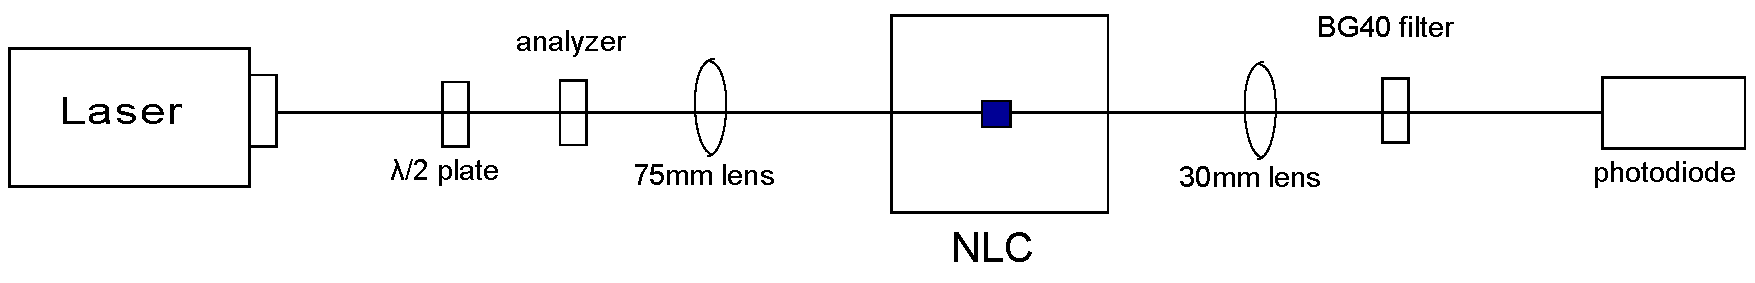
\includegraphics[width=1.0\textwidth]{graphics/setup_2ndharmonic}
  \caption{Setup to generate frequency doubled light}
  \label{fig:setup_2ndharmonic}
\end{figure}
We use a plano-convex lens with focal length $f = \unit[75]{mm}$ to focus the laser beam into a heatable non-linear potassium niobate crystal (NLC) and an achromatic lens (focal length $f=\unit[30]{mm}$) to collimate the light transmitted by this crystal. Behind the lens a BG40 glass filter is placed in order to filter out the infrared fundamental wave. The photodiode is used to measure the second harmonic wave's power. We increase the temperature of the crystal up to 36�C and optimize our alignment until the frequency doubled light has a power of $P_\textrm{harmonic} = \unit[(22.0 \pm 0.1)]{mW}$.

In order to check our setup we calculate the beam waist and Rayleigh length of the laser beam in the crystal. Before the lens the collimated laser beam has the size $2\omega_0 = \unit[(3.5 \pm 0.5)]{mm}$. The lens used for focussing a refractive index of approximately $n = \unit[2.2]{}$ and the length of the crystal is given by $l=\unit[5]{mm}$.
\begin{figure}[H]
  \centering
  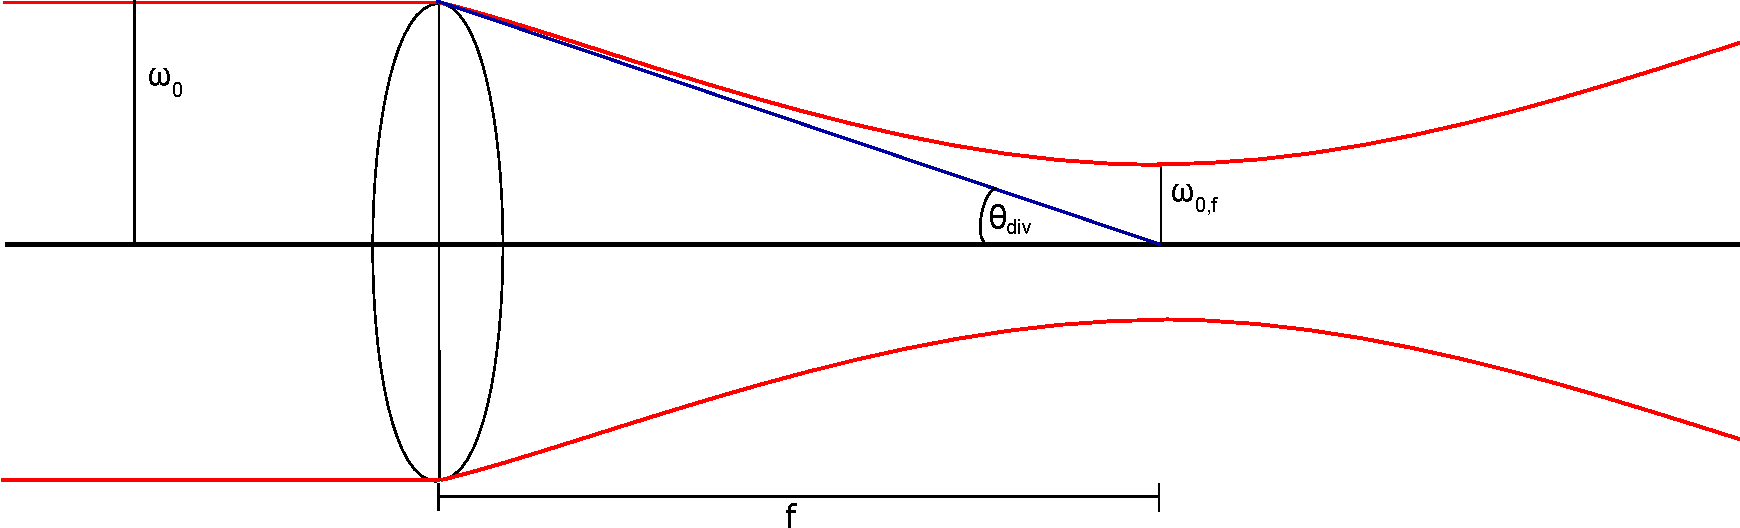
\includegraphics[width=1.0\textwidth]{graphics/ana_gauss}
  \caption{Illustration of the gauss beam}
  \label{fig:ana_gauss}
\end{figure}
Because we assume that the radius of the beam waist in the crystal is the same as if the beam would propagate in air the following equation holds for the beam (see section XXX):
\begin{align*}
\theta_\textrm{div} = \arctan\left(\frac{\lambda}{\pi\omega_{0,\textrm{f}}}\right)
\end{align*}
where $2\omega_{0,\textrm{f}}$ is the beam diameter in the crystal and $\lambda$ is the wavelength of the laser beam. As shown in figure \ref{fig:ana_gauss} we know:
\begin{align*}
\theta_\textrm{div} = \arctan\left(\frac{\omega_0}{f}\right)
\end{align*}
and therefore
\begin{align}
\omega_{0,\textrm{f}} = \frac{\lambda f}{\pi\omega_0} \hspace{2cm} \Delta \omega_{0,\textrm{f}} = \frac{\lambda f}{\pi\omega_0^2}\Delta \omega_0
\end{align}
According to section XXX the length of the rayleigh zone (\textbf{REMARK: IN THIS SECTION 'RAYLEIGH ZONE' SHOULD BE EXPLAINED}) is given by:
\begin{align}
z_0 = \frac{\pi n\omega_{0,\textrm{f}}^2}{\lambda} \hspace{2cm} \Delta z_0 = \frac{2\pi n\omega_{0,\textrm{f}}}{\lambda}\Delta \omega_{0,\textrm{f}}
\end{align}
Additionally we define the relation $\zeta$ by
\begin{align}
\zeta = \frac{l}{2z_0} \hspace{2cm} \Delta \zeta = \frac{l}{2z_0^2}\Delta z_0
\end{align}
plugging in our values yields:
\begin{align}
\omega_{0,\textrm{f}} &= \unit[(0.013 \pm 0.002)]{mm} \\
\notag z_0 &=  \unit[(1.2 \pm 0.4)]{mm}\\
\notag \zeta &= \unit[(2.1 \pm 0.7)]{}
\end{align}
The Boyd-Kleinman condition for the optimal efficiency of second-harmonic generation is $\zeta = \unit[2.84]{}$. The focus of our achromat is therefore not optimal but sufficient for our purposes. The optimal focus length would be given by:
\begin{align}
f_\textrm{optimal} = \sqrt{\frac{\pi l \omega^2_0}{2n\lambda\zeta}} \hspace{1.5cm} \Delta f_\textrm{optimal} = \sqrt{\frac{2\pi l}{n\lambda\zeta}}\Delta\omega_0
\end{align}
which in our case yields:
\begin{align}
f_\textrm{optimal} = \unit[(63 \pm 9)]{mm}
\end{align}
\subsection{Properties of second-harmonic generation}\label{subsec:ana_props_2ndharmonic}
\subsubsection{Dependency on temperature}\label{subsubsec:ana_temp_dep}
Now we want to examine the dependency of the second harmonic's power on the temperature of the NLC. Therefore we use the same setup as above. The temperature of the NLC is lowered to $\unit[27]{�C}$ and then raised in steps of \unit[0.2]{�C}. For each temperature of the NLC we measure the power of the second harmonic. The laser input current is set constantly to $I=\unit[(280.0 \pm 0.5)]{mA}$. The recorded data is shown in table \ref{tab:ana_temp_dep} in the appendix and plotted in figure \ref{fig:ana_temp_dep}.
\begin{figure}[H]
  \resizebox{0.8\textwidth}{!}{
    \begin{tikzpicture}[gnuplot]
%% generated with GNUPLOT 4.4p0 (Lua 5.1.4; terminal rev. 97, script rev. 96a)
%% 25.04.2010 13:37:09
\gpcolor{gp lt color border}
\gpsetlinetype{gp lt border}
\gpsetlinewidth{1.00}
\draw[gp path] (2.424,0.985)--(2.604,0.985);
\draw[gp path] (12.039,0.985)--(11.859,0.985);
\node[gp node right] at (2.240,0.985) { 1};
\draw[gp path] (2.424,2.267)--(2.514,2.267);
\draw[gp path] (12.039,2.267)--(11.949,2.267);
\draw[gp path] (2.424,2.834)--(2.604,2.834);
\draw[gp path] (12.039,2.834)--(11.859,2.834);
\node[gp node right] at (2.240,2.834) { 2.71828};
\draw[gp path] (2.424,4.116)--(2.514,4.116);
\draw[gp path] (12.039,4.116)--(11.949,4.116);
\draw[gp path] (2.424,4.683)--(2.604,4.683);
\draw[gp path] (12.039,4.683)--(11.859,4.683);
\node[gp node right] at (2.240,4.683) { 7.38906};
\draw[gp path] (2.424,5.965)--(2.514,5.965);
\draw[gp path] (12.039,5.965)--(11.949,5.965);
\draw[gp path] (2.424,6.532)--(2.604,6.532);
\draw[gp path] (12.039,6.532)--(11.859,6.532);
\node[gp node right] at (2.240,6.532) { 20.0855};
\draw[gp path] (2.424,7.814)--(2.514,7.814);
\draw[gp path] (12.039,7.814)--(11.949,7.814);
\draw[gp path] (2.424,8.381)--(2.604,8.381);
\draw[gp path] (12.039,8.381)--(11.859,8.381);
\node[gp node right] at (2.240,8.381) { 54.5982};
\draw[gp path] (2.424,0.985)--(2.424,1.165);
\draw[gp path] (2.424,8.381)--(2.424,8.201);
\node[gp node center] at (2.424,0.677) { 26};
\draw[gp path] (3.626,0.985)--(3.626,1.165);
\draw[gp path] (3.626,8.381)--(3.626,8.201);
\node[gp node center] at (3.626,0.677) { 28};
\draw[gp path] (4.828,0.985)--(4.828,1.165);
\draw[gp path] (4.828,8.381)--(4.828,8.201);
\node[gp node center] at (4.828,0.677) { 30};
\draw[gp path] (6.030,0.985)--(6.030,1.165);
\draw[gp path] (6.030,8.381)--(6.030,8.201);
\node[gp node center] at (6.030,0.677) { 32};
\draw[gp path] (7.232,0.985)--(7.232,1.165);
\draw[gp path] (7.232,8.381)--(7.232,8.201);
\node[gp node center] at (7.232,0.677) { 34};
\draw[gp path] (8.433,0.985)--(8.433,1.165);
\draw[gp path] (8.433,8.381)--(8.433,8.201);
\node[gp node center] at (8.433,0.677) { 36};
\draw[gp path] (9.635,0.985)--(9.635,1.165);
\draw[gp path] (9.635,8.381)--(9.635,8.201);
\node[gp node center] at (9.635,0.677) { 38};
\draw[gp path] (10.837,0.985)--(10.837,1.165);
\draw[gp path] (10.837,8.381)--(10.837,8.201);
\node[gp node center] at (10.837,0.677) { 40};
\draw[gp path] (12.039,0.985)--(12.039,1.165);
\draw[gp path] (12.039,8.381)--(12.039,8.201);
\node[gp node center] at (12.039,0.677) { 42};
\draw[gp path] (2.424,8.381)--(2.424,0.985)--(12.039,0.985)--(12.039,8.381)--cycle;
\node[gp node center,rotate=-270] at (0.430,4.683) {2nd harmonic power [$\mu$W]};
\node[gp node center] at (7.231,0.215) {Temperature [�C]};
\node[gp node right] at (10.571,8.047) {Measured Data};
\gpcolor{gp lt color 0}
\gpsetlinetype{gp lt plot 0}
\draw[gp path] (10.755,8.047)--(11.671,8.047);
\draw[gp path] (10.755,8.137)--(10.755,7.957);
\draw[gp path] (11.671,8.137)--(11.671,7.957);
\draw[gp path] (3.025,1.872)--(3.025,1.904);
\draw[gp path] (2.935,1.872)--(3.115,1.872);
\draw[gp path] (2.935,1.904)--(3.115,1.904);
\draw[gp path] (3.145,1.861)--(3.145,1.893);
\draw[gp path] (3.055,1.861)--(3.235,1.861);
\draw[gp path] (3.055,1.893)--(3.235,1.893);
\draw[gp path] (3.265,1.872)--(3.265,1.904);
\draw[gp path] (3.175,1.872)--(3.355,1.872);
\draw[gp path] (3.175,1.904)--(3.355,1.904);
\draw[gp path] (3.386,1.884)--(3.386,1.916);
\draw[gp path] (3.296,1.884)--(3.476,1.884);
\draw[gp path] (3.296,1.916)--(3.476,1.916);
\draw[gp path] (3.506,1.884)--(3.506,1.916);
\draw[gp path] (3.416,1.884)--(3.596,1.884);
\draw[gp path] (3.416,1.916)--(3.596,1.916);
\draw[gp path] (3.626,1.884)--(3.626,1.916);
\draw[gp path] (3.536,1.884)--(3.716,1.884);
\draw[gp path] (3.536,1.916)--(3.716,1.916);
\draw[gp path] (3.746,1.872)--(3.746,1.904);
\draw[gp path] (3.656,1.872)--(3.836,1.872);
\draw[gp path] (3.656,1.904)--(3.836,1.904);
\draw[gp path] (3.866,1.872)--(3.866,1.904);
\draw[gp path] (3.776,1.872)--(3.956,1.872);
\draw[gp path] (3.776,1.904)--(3.956,1.904);
\draw[gp path] (3.986,1.872)--(3.986,1.904);
\draw[gp path] (3.896,1.872)--(4.076,1.872);
\draw[gp path] (3.896,1.904)--(4.076,1.904);
\draw[gp path] (4.107,1.884)--(4.107,1.916);
\draw[gp path] (4.017,1.884)--(4.197,1.884);
\draw[gp path] (4.017,1.916)--(4.197,1.916);
\draw[gp path] (4.227,1.906)--(4.227,1.938);
\draw[gp path] (4.137,1.906)--(4.317,1.906);
\draw[gp path] (4.137,1.938)--(4.317,1.938);
\draw[gp path] (4.347,1.906)--(4.347,1.938);
\draw[gp path] (4.257,1.906)--(4.437,1.906);
\draw[gp path] (4.257,1.938)--(4.437,1.938);
\draw[gp path] (4.467,1.895)--(4.467,1.927);
\draw[gp path] (4.377,1.895)--(4.557,1.895);
\draw[gp path] (4.377,1.927)--(4.557,1.927);
\draw[gp path] (4.587,1.884)--(4.587,1.916);
\draw[gp path] (4.497,1.884)--(4.677,1.884);
\draw[gp path] (4.497,1.916)--(4.677,1.916);
\draw[gp path] (4.708,1.872)--(4.708,1.904);
\draw[gp path] (4.618,1.872)--(4.798,1.872);
\draw[gp path] (4.618,1.904)--(4.798,1.904);
\draw[gp path] (4.828,1.884)--(4.828,1.916);
\draw[gp path] (4.738,1.884)--(4.918,1.884);
\draw[gp path] (4.738,1.916)--(4.918,1.916);
\draw[gp path] (4.948,1.906)--(4.948,1.938);
\draw[gp path] (4.858,1.906)--(5.038,1.906);
\draw[gp path] (4.858,1.938)--(5.038,1.938);
\draw[gp path] (5.068,1.929)--(5.068,1.960);
\draw[gp path] (4.978,1.929)--(5.158,1.929);
\draw[gp path] (4.978,1.960)--(5.158,1.960);
\draw[gp path] (5.188,1.929)--(5.188,1.960);
\draw[gp path] (5.098,1.929)--(5.278,1.929);
\draw[gp path] (5.098,1.960)--(5.278,1.960);
\draw[gp path] (5.309,1.951)--(5.309,1.981);
\draw[gp path] (5.219,1.951)--(5.399,1.951);
\draw[gp path] (5.219,1.981)--(5.399,1.981);
\draw[gp path] (5.429,1.906)--(5.429,1.938);
\draw[gp path] (5.339,1.906)--(5.519,1.906);
\draw[gp path] (5.339,1.938)--(5.519,1.938);
\draw[gp path] (5.549,1.895)--(5.549,1.927);
\draw[gp path] (5.459,1.895)--(5.639,1.895);
\draw[gp path] (5.459,1.927)--(5.639,1.927);
\draw[gp path] (5.669,1.917)--(5.669,1.949);
\draw[gp path] (5.579,1.917)--(5.759,1.917);
\draw[gp path] (5.579,1.949)--(5.759,1.949);
\draw[gp path] (5.789,1.951)--(5.789,1.981);
\draw[gp path] (5.699,1.951)--(5.879,1.951);
\draw[gp path] (5.699,1.981)--(5.879,1.981);
\draw[gp path] (5.909,1.983)--(5.909,2.014);
\draw[gp path] (5.819,1.983)--(5.999,1.983);
\draw[gp path] (5.819,2.014)--(5.999,2.014);
\draw[gp path] (6.030,1.972)--(6.030,2.003);
\draw[gp path] (5.940,1.972)--(6.120,1.972);
\draw[gp path] (5.940,2.003)--(6.120,2.003);
\draw[gp path] (6.150,1.940)--(6.150,1.971);
\draw[gp path] (6.060,1.940)--(6.240,1.940);
\draw[gp path] (6.060,1.971)--(6.240,1.971);
\draw[gp path] (6.270,1.906)--(6.270,1.938);
\draw[gp path] (6.180,1.906)--(6.360,1.906);
\draw[gp path] (6.180,1.938)--(6.360,1.938);
\draw[gp path] (6.390,1.917)--(6.390,1.949);
\draw[gp path] (6.300,1.917)--(6.480,1.917);
\draw[gp path] (6.300,1.949)--(6.480,1.949);
\draw[gp path] (6.510,1.972)--(6.510,2.003);
\draw[gp path] (6.420,1.972)--(6.600,1.972);
\draw[gp path] (6.420,2.003)--(6.600,2.003);
\draw[gp path] (6.631,2.047)--(6.631,2.076);
\draw[gp path] (6.541,2.047)--(6.721,2.047);
\draw[gp path] (6.541,2.076)--(6.721,2.076);
\draw[gp path] (6.751,2.068)--(6.751,2.096);
\draw[gp path] (6.661,2.068)--(6.841,2.068);
\draw[gp path] (6.661,2.096)--(6.841,2.096);
\draw[gp path] (6.871,2.047)--(6.871,2.076);
\draw[gp path] (6.781,2.047)--(6.961,2.047);
\draw[gp path] (6.781,2.076)--(6.961,2.076);
\draw[gp path] (6.991,1.983)--(6.991,2.014);
\draw[gp path] (6.901,1.983)--(7.081,1.983);
\draw[gp path] (6.901,2.014)--(7.081,2.014);
\draw[gp path] (7.111,1.972)--(7.111,2.003);
\draw[gp path] (7.021,1.972)--(7.201,1.972);
\draw[gp path] (7.021,2.003)--(7.201,2.003);
\draw[gp path] (7.232,2.036)--(7.232,2.066);
\draw[gp path] (7.142,2.036)--(7.322,2.036);
\draw[gp path] (7.142,2.066)--(7.322,2.066);
\draw[gp path] (7.352,2.128)--(7.352,2.156);
\draw[gp path] (7.262,2.128)--(7.442,2.128);
\draw[gp path] (7.262,2.156)--(7.442,2.156);
\draw[gp path] (7.472,2.177)--(7.472,2.205);
\draw[gp path] (7.382,2.177)--(7.562,2.177);
\draw[gp path] (7.382,2.205)--(7.562,2.205);
\draw[gp path] (7.592,2.168)--(7.592,2.195);
\draw[gp path] (7.502,2.168)--(7.682,2.168);
\draw[gp path] (7.502,2.195)--(7.682,2.195);
\draw[gp path] (7.712,2.225)--(7.712,2.252);
\draw[gp path] (7.622,2.225)--(7.802,2.225);
\draw[gp path] (7.622,2.252)--(7.802,2.252);
\draw[gp path] (7.832,2.720)--(7.832,2.740);
\draw[gp path] (7.742,2.720)--(7.922,2.720);
\draw[gp path] (7.742,2.740)--(7.922,2.740);
\draw[gp path] (7.953,3.702)--(7.953,3.714);
\draw[gp path] (7.863,3.702)--(8.043,3.702);
\draw[gp path] (7.863,3.714)--(8.043,3.714);
\draw[gp path] (8.073,4.677)--(8.073,4.684);
\draw[gp path] (7.983,4.677)--(8.163,4.677);
\draw[gp path] (7.983,4.684)--(8.163,4.684);
\draw[gp path] (8.193,5.653)--(8.193,5.657);
\draw[gp path] (8.103,5.653)--(8.283,5.653);
\draw[gp path] (8.103,5.657)--(8.283,5.657);
\draw[gp path] (8.313,6.389)--(8.313,6.391);
\draw[gp path] (8.223,6.389)--(8.403,6.389);
\draw[gp path] (8.223,6.391)--(8.403,6.391);
\draw[gp path] (8.433,6.797)--(8.433,6.800);
\draw[gp path] (8.343,6.797)--(8.523,6.797);
\draw[gp path] (8.343,6.800)--(8.523,6.800);
\draw[gp path] (8.554,7.050)--(8.554,7.052);
\draw[gp path] (8.464,7.050)--(8.644,7.050);
\draw[gp path] (8.464,7.052)--(8.644,7.052);
\draw[gp path] (8.674,7.098)--(8.674,7.100);
\draw[gp path] (8.584,7.098)--(8.764,7.098);
\draw[gp path] (8.584,7.100)--(8.764,7.100);
\draw[gp path] (8.794,6.837)--(8.794,6.839);
\draw[gp path] (8.704,6.837)--(8.884,6.837);
\draw[gp path] (8.704,6.839)--(8.884,6.839);
\draw[gp path] (8.914,6.559)--(8.914,6.562);
\draw[gp path] (8.824,6.559)--(9.004,6.559);
\draw[gp path] (8.824,6.562)--(9.004,6.562);
\draw[gp path] (9.034,5.809)--(9.034,5.813);
\draw[gp path] (8.944,5.809)--(9.124,5.809);
\draw[gp path] (8.944,5.813)--(9.124,5.813);
\draw[gp path] (9.155,4.827)--(9.155,4.833);
\draw[gp path] (9.065,4.827)--(9.245,4.827);
\draw[gp path] (9.065,4.833)--(9.245,4.833);
\draw[gp path] (9.275,3.632)--(9.275,3.645);
\draw[gp path] (9.185,3.632)--(9.365,3.632);
\draw[gp path] (9.185,3.645)--(9.365,3.645);
\draw[gp path] (9.395,2.669)--(9.395,2.690);
\draw[gp path] (9.305,2.669)--(9.485,2.669);
\draw[gp path] (9.305,2.690)--(9.485,2.690);
\draw[gp path] (9.515,2.158)--(9.515,2.185);
\draw[gp path] (9.425,2.158)--(9.605,2.158);
\draw[gp path] (9.425,2.185)--(9.605,2.185);
\draw[gp path] (9.635,2.431)--(9.635,2.455);
\draw[gp path] (9.545,2.431)--(9.725,2.431);
\draw[gp path] (9.545,2.455)--(9.725,2.455);
\draw[gp path] (9.755,2.593)--(9.755,2.615);
\draw[gp path] (9.665,2.593)--(9.845,2.593);
\draw[gp path] (9.665,2.615)--(9.845,2.615);
\draw[gp path] (9.876,2.593)--(9.876,2.615);
\draw[gp path] (9.786,2.593)--(9.966,2.593);
\draw[gp path] (9.786,2.615)--(9.966,2.615);
\draw[gp path] (9.996,2.344)--(9.996,2.369);
\draw[gp path] (9.906,2.344)--(10.086,2.344);
\draw[gp path] (9.906,2.369)--(10.086,2.369);
\draw[gp path] (10.116,2.057)--(10.116,2.086);
\draw[gp path] (10.026,2.057)--(10.206,2.057);
\draw[gp path] (10.026,2.086)--(10.206,2.086);
\draw[gp path] (10.236,1.838)--(10.236,1.870);
\draw[gp path] (10.146,1.838)--(10.326,1.838);
\draw[gp path] (10.146,1.870)--(10.326,1.870);
\draw[gp path] (10.356,1.951)--(10.356,1.981);
\draw[gp path] (10.266,1.951)--(10.446,1.951);
\draw[gp path] (10.266,1.981)--(10.446,1.981);
\draw[gp path] (10.477,2.057)--(10.477,2.086);
\draw[gp path] (10.387,2.057)--(10.567,2.057);
\draw[gp path] (10.387,2.086)--(10.567,2.086);
\draw[gp path] (10.597,2.057)--(10.597,2.086);
\draw[gp path] (10.507,2.057)--(10.687,2.057);
\draw[gp path] (10.507,2.086)--(10.687,2.086);
\draw[gp path] (10.717,2.057)--(10.717,2.086);
\draw[gp path] (10.627,2.057)--(10.807,2.057);
\draw[gp path] (10.627,2.086)--(10.807,2.086);
\draw[gp path] (10.837,1.951)--(10.837,1.981);
\draw[gp path] (10.747,1.951)--(10.927,1.951);
\draw[gp path] (10.747,1.981)--(10.927,1.981);
\draw[gp path] (2.965,1.888)--(3.085,1.888);
\draw[gp path] (2.965,1.798)--(2.965,1.978);
\draw[gp path] (3.085,1.798)--(3.085,1.978);
\draw[gp path] (3.085,1.877)--(3.205,1.877);
\draw[gp path] (3.085,1.787)--(3.085,1.967);
\draw[gp path] (3.205,1.787)--(3.205,1.967);
\draw[gp path] (3.205,1.888)--(3.325,1.888);
\draw[gp path] (3.205,1.798)--(3.205,1.978);
\draw[gp path] (3.325,1.798)--(3.325,1.978);
\draw[gp path] (3.325,1.900)--(3.446,1.900);
\draw[gp path] (3.325,1.810)--(3.325,1.990);
\draw[gp path] (3.446,1.810)--(3.446,1.990);
\draw[gp path] (3.446,1.900)--(3.566,1.900);
\draw[gp path] (3.446,1.810)--(3.446,1.990);
\draw[gp path] (3.566,1.810)--(3.566,1.990);
\draw[gp path] (3.566,1.900)--(3.686,1.900);
\draw[gp path] (3.566,1.810)--(3.566,1.990);
\draw[gp path] (3.686,1.810)--(3.686,1.990);
\draw[gp path] (3.686,1.888)--(3.806,1.888);
\draw[gp path] (3.686,1.798)--(3.686,1.978);
\draw[gp path] (3.806,1.798)--(3.806,1.978);
\draw[gp path] (3.806,1.888)--(3.926,1.888);
\draw[gp path] (3.806,1.798)--(3.806,1.978);
\draw[gp path] (3.926,1.798)--(3.926,1.978);
\draw[gp path] (3.926,1.888)--(4.047,1.888);
\draw[gp path] (3.926,1.798)--(3.926,1.978);
\draw[gp path] (4.047,1.798)--(4.047,1.978);
\draw[gp path] (4.047,1.900)--(4.167,1.900);
\draw[gp path] (4.047,1.810)--(4.047,1.990);
\draw[gp path] (4.167,1.810)--(4.167,1.990);
\draw[gp path] (4.167,1.922)--(4.287,1.922);
\draw[gp path] (4.167,1.832)--(4.167,2.012);
\draw[gp path] (4.287,1.832)--(4.287,2.012);
\draw[gp path] (4.287,1.922)--(4.407,1.922);
\draw[gp path] (4.287,1.832)--(4.287,2.012);
\draw[gp path] (4.407,1.832)--(4.407,2.012);
\draw[gp path] (4.407,1.911)--(4.527,1.911);
\draw[gp path] (4.407,1.821)--(4.407,2.001);
\draw[gp path] (4.527,1.821)--(4.527,2.001);
\draw[gp path] (4.527,1.900)--(4.647,1.900);
\draw[gp path] (4.527,1.810)--(4.527,1.990);
\draw[gp path] (4.647,1.810)--(4.647,1.990);
\draw[gp path] (4.647,1.888)--(4.768,1.888);
\draw[gp path] (4.647,1.798)--(4.647,1.978);
\draw[gp path] (4.768,1.798)--(4.768,1.978);
\draw[gp path] (4.768,1.900)--(4.888,1.900);
\draw[gp path] (4.768,1.810)--(4.768,1.990);
\draw[gp path] (4.888,1.810)--(4.888,1.990);
\draw[gp path] (4.888,1.922)--(5.008,1.922);
\draw[gp path] (4.888,1.832)--(4.888,2.012);
\draw[gp path] (5.008,1.832)--(5.008,2.012);
\draw[gp path] (5.008,1.944)--(5.128,1.944);
\draw[gp path] (5.008,1.854)--(5.008,2.034);
\draw[gp path] (5.128,1.854)--(5.128,2.034);
\draw[gp path] (5.128,1.944)--(5.248,1.944);
\draw[gp path] (5.128,1.854)--(5.128,2.034);
\draw[gp path] (5.248,1.854)--(5.248,2.034);
\draw[gp path] (5.248,1.966)--(5.369,1.966);
\draw[gp path] (5.248,1.876)--(5.248,2.056);
\draw[gp path] (5.369,1.876)--(5.369,2.056);
\draw[gp path] (5.369,1.922)--(5.489,1.922);
\draw[gp path] (5.369,1.832)--(5.369,2.012);
\draw[gp path] (5.489,1.832)--(5.489,2.012);
\draw[gp path] (5.489,1.911)--(5.609,1.911);
\draw[gp path] (5.489,1.821)--(5.489,2.001);
\draw[gp path] (5.609,1.821)--(5.609,2.001);
\draw[gp path] (5.609,1.933)--(5.729,1.933);
\draw[gp path] (5.609,1.843)--(5.609,2.023);
\draw[gp path] (5.729,1.843)--(5.729,2.023);
\draw[gp path] (5.729,1.966)--(5.849,1.966);
\draw[gp path] (5.729,1.876)--(5.729,2.056);
\draw[gp path] (5.849,1.876)--(5.849,2.056);
\draw[gp path] (5.849,1.998)--(5.970,1.998);
\draw[gp path] (5.849,1.908)--(5.849,2.088);
\draw[gp path] (5.970,1.908)--(5.970,2.088);
\draw[gp path] (5.970,1.988)--(6.090,1.988);
\draw[gp path] (5.970,1.898)--(5.970,2.078);
\draw[gp path] (6.090,1.898)--(6.090,2.078);
\draw[gp path] (6.090,1.955)--(6.210,1.955);
\draw[gp path] (6.090,1.865)--(6.090,2.045);
\draw[gp path] (6.210,1.865)--(6.210,2.045);
\draw[gp path] (6.210,1.922)--(6.330,1.922);
\draw[gp path] (6.210,1.832)--(6.210,2.012);
\draw[gp path] (6.330,1.832)--(6.330,2.012);
\draw[gp path] (6.330,1.933)--(6.450,1.933);
\draw[gp path] (6.330,1.843)--(6.330,2.023);
\draw[gp path] (6.450,1.843)--(6.450,2.023);
\draw[gp path] (6.450,1.988)--(6.570,1.988);
\draw[gp path] (6.450,1.898)--(6.450,2.078);
\draw[gp path] (6.570,1.898)--(6.570,2.078);
\draw[gp path] (6.570,2.062)--(6.691,2.062);
\draw[gp path] (6.570,1.972)--(6.570,2.152);
\draw[gp path] (6.691,1.972)--(6.691,2.152);
\draw[gp path] (6.691,2.082)--(6.811,2.082);
\draw[gp path] (6.691,1.992)--(6.691,2.172);
\draw[gp path] (6.811,1.992)--(6.811,2.172);
\draw[gp path] (6.811,2.062)--(6.931,2.062);
\draw[gp path] (6.811,1.972)--(6.811,2.152);
\draw[gp path] (6.931,1.972)--(6.931,2.152);
\draw[gp path] (6.931,1.998)--(7.051,1.998);
\draw[gp path] (6.931,1.908)--(6.931,2.088);
\draw[gp path] (7.051,1.908)--(7.051,2.088);
\draw[gp path] (7.051,1.988)--(7.171,1.988);
\draw[gp path] (7.051,1.898)--(7.051,2.078);
\draw[gp path] (7.171,1.898)--(7.171,2.078);
\draw[gp path] (7.171,2.051)--(7.292,2.051);
\draw[gp path] (7.171,1.961)--(7.171,2.141);
\draw[gp path] (7.292,1.961)--(7.292,2.141);
\draw[gp path] (7.292,2.142)--(7.412,2.142);
\draw[gp path] (7.292,2.052)--(7.292,2.232);
\draw[gp path] (7.412,2.052)--(7.412,2.232);
\draw[gp path] (7.412,2.191)--(7.532,2.191);
\draw[gp path] (7.412,2.101)--(7.412,2.281);
\draw[gp path] (7.532,2.101)--(7.532,2.281);
\draw[gp path] (7.532,2.181)--(7.652,2.181);
\draw[gp path] (7.532,2.091)--(7.532,2.271);
\draw[gp path] (7.652,2.091)--(7.652,2.271);
\draw[gp path] (7.652,2.239)--(7.772,2.239);
\draw[gp path] (7.652,2.149)--(7.652,2.329);
\draw[gp path] (7.772,2.149)--(7.772,2.329);
\draw[gp path] (7.772,2.730)--(7.893,2.730);
\draw[gp path] (7.772,2.640)--(7.772,2.820);
\draw[gp path] (7.893,2.640)--(7.893,2.820);
\draw[gp path] (7.893,3.708)--(8.013,3.708);
\draw[gp path] (7.893,3.618)--(7.893,3.798);
\draw[gp path] (8.013,3.618)--(8.013,3.798);
\draw[gp path] (8.013,4.681)--(8.133,4.681);
\draw[gp path] (8.013,4.591)--(8.013,4.771);
\draw[gp path] (8.133,4.591)--(8.133,4.771);
\draw[gp path] (8.133,5.655)--(8.253,5.655);
\draw[gp path] (8.133,5.565)--(8.133,5.745);
\draw[gp path] (8.253,5.565)--(8.253,5.745);
\draw[gp path] (8.253,6.390)--(8.373,6.390);
\draw[gp path] (8.253,6.300)--(8.253,6.480);
\draw[gp path] (8.373,6.300)--(8.373,6.480);
\draw[gp path] (8.373,6.799)--(8.493,6.799);
\draw[gp path] (8.373,6.709)--(8.373,6.889);
\draw[gp path] (8.493,6.709)--(8.493,6.889);
\draw[gp path] (8.493,7.051)--(8.614,7.051);
\draw[gp path] (8.493,6.961)--(8.493,7.141);
\draw[gp path] (8.614,6.961)--(8.614,7.141);
\draw[gp path] (8.614,7.099)--(8.734,7.099);
\draw[gp path] (8.614,7.009)--(8.614,7.189);
\draw[gp path] (8.734,7.009)--(8.734,7.189);
\draw[gp path] (8.734,6.838)--(8.854,6.838);
\draw[gp path] (8.734,6.748)--(8.734,6.928);
\draw[gp path] (8.854,6.748)--(8.854,6.928);
\draw[gp path] (8.854,6.561)--(8.974,6.561);
\draw[gp path] (8.854,6.471)--(8.854,6.651);
\draw[gp path] (8.974,6.471)--(8.974,6.651);
\draw[gp path] (8.974,5.811)--(9.094,5.811);
\draw[gp path] (8.974,5.721)--(8.974,5.901);
\draw[gp path] (9.094,5.721)--(9.094,5.901);
\draw[gp path] (9.094,4.830)--(9.215,4.830);
\draw[gp path] (9.094,4.740)--(9.094,4.920);
\draw[gp path] (9.215,4.740)--(9.215,4.920);
\draw[gp path] (9.215,3.638)--(9.335,3.638);
\draw[gp path] (9.215,3.548)--(9.215,3.728);
\draw[gp path] (9.335,3.548)--(9.335,3.728);
\draw[gp path] (9.335,2.679)--(9.455,2.679);
\draw[gp path] (9.335,2.589)--(9.335,2.769);
\draw[gp path] (9.455,2.589)--(9.455,2.769);
\draw[gp path] (9.455,2.172)--(9.575,2.172);
\draw[gp path] (9.455,2.082)--(9.455,2.262);
\draw[gp path] (9.575,2.082)--(9.575,2.262);
\draw[gp path] (9.575,2.443)--(9.695,2.443);
\draw[gp path] (9.575,2.353)--(9.575,2.533);
\draw[gp path] (9.695,2.353)--(9.695,2.533);
\draw[gp path] (9.695,2.604)--(9.816,2.604);
\draw[gp path] (9.695,2.514)--(9.695,2.694);
\draw[gp path] (9.816,2.514)--(9.816,2.694);
\draw[gp path] (9.816,2.604)--(9.936,2.604);
\draw[gp path] (9.816,2.514)--(9.816,2.694);
\draw[gp path] (9.936,2.514)--(9.936,2.694);
\draw[gp path] (9.936,2.357)--(10.056,2.357);
\draw[gp path] (9.936,2.267)--(9.936,2.447);
\draw[gp path] (10.056,2.267)--(10.056,2.447);
\draw[gp path] (10.056,2.072)--(10.176,2.072);
\draw[gp path] (10.056,1.982)--(10.056,2.162);
\draw[gp path] (10.176,1.982)--(10.176,2.162);
\draw[gp path] (10.176,1.854)--(10.296,1.854);
\draw[gp path] (10.176,1.764)--(10.176,1.944);
\draw[gp path] (10.296,1.764)--(10.296,1.944);
\draw[gp path] (10.296,1.966)--(10.416,1.966);
\draw[gp path] (10.296,1.876)--(10.296,2.056);
\draw[gp path] (10.416,1.876)--(10.416,2.056);
\draw[gp path] (10.416,2.072)--(10.537,2.072);
\draw[gp path] (10.416,1.982)--(10.416,2.162);
\draw[gp path] (10.537,1.982)--(10.537,2.162);
\draw[gp path] (10.537,2.072)--(10.657,2.072);
\draw[gp path] (10.537,1.982)--(10.537,2.162);
\draw[gp path] (10.657,1.982)--(10.657,2.162);
\draw[gp path] (10.657,2.072)--(10.777,2.072);
\draw[gp path] (10.657,1.982)--(10.657,2.162);
\draw[gp path] (10.777,1.982)--(10.777,2.162);
\draw[gp path] (10.777,1.966)--(10.897,1.966);
\draw[gp path] (10.777,1.876)--(10.777,2.056);
\draw[gp path] (10.897,1.876)--(10.897,2.056);
\gpsetpointsize{4.00}
\gppoint{gp mark 1}{(3.025,1.888)}
\gppoint{gp mark 1}{(3.145,1.877)}
\gppoint{gp mark 1}{(3.265,1.888)}
\gppoint{gp mark 1}{(3.386,1.900)}
\gppoint{gp mark 1}{(3.506,1.900)}
\gppoint{gp mark 1}{(3.626,1.900)}
\gppoint{gp mark 1}{(3.746,1.888)}
\gppoint{gp mark 1}{(3.866,1.888)}
\gppoint{gp mark 1}{(3.986,1.888)}
\gppoint{gp mark 1}{(4.107,1.900)}
\gppoint{gp mark 1}{(4.227,1.922)}
\gppoint{gp mark 1}{(4.347,1.922)}
\gppoint{gp mark 1}{(4.467,1.911)}
\gppoint{gp mark 1}{(4.587,1.900)}
\gppoint{gp mark 1}{(4.708,1.888)}
\gppoint{gp mark 1}{(4.828,1.900)}
\gppoint{gp mark 1}{(4.948,1.922)}
\gppoint{gp mark 1}{(5.068,1.944)}
\gppoint{gp mark 1}{(5.188,1.944)}
\gppoint{gp mark 1}{(5.309,1.966)}
\gppoint{gp mark 1}{(5.429,1.922)}
\gppoint{gp mark 1}{(5.549,1.911)}
\gppoint{gp mark 1}{(5.669,1.933)}
\gppoint{gp mark 1}{(5.789,1.966)}
\gppoint{gp mark 1}{(5.909,1.998)}
\gppoint{gp mark 1}{(6.030,1.988)}
\gppoint{gp mark 1}{(6.150,1.955)}
\gppoint{gp mark 1}{(6.270,1.922)}
\gppoint{gp mark 1}{(6.390,1.933)}
\gppoint{gp mark 1}{(6.510,1.988)}
\gppoint{gp mark 1}{(6.631,2.062)}
\gppoint{gp mark 1}{(6.751,2.082)}
\gppoint{gp mark 1}{(6.871,2.062)}
\gppoint{gp mark 1}{(6.991,1.998)}
\gppoint{gp mark 1}{(7.111,1.988)}
\gppoint{gp mark 1}{(7.232,2.051)}
\gppoint{gp mark 1}{(7.352,2.142)}
\gppoint{gp mark 1}{(7.472,2.191)}
\gppoint{gp mark 1}{(7.592,2.181)}
\gppoint{gp mark 1}{(7.712,2.239)}
\gppoint{gp mark 1}{(7.832,2.730)}
\gppoint{gp mark 1}{(7.953,3.708)}
\gppoint{gp mark 1}{(8.073,4.681)}
\gppoint{gp mark 1}{(8.193,5.655)}
\gppoint{gp mark 1}{(8.313,6.390)}
\gppoint{gp mark 1}{(8.433,6.799)}
\gppoint{gp mark 1}{(8.554,7.051)}
\gppoint{gp mark 1}{(8.674,7.099)}
\gppoint{gp mark 1}{(8.794,6.838)}
\gppoint{gp mark 1}{(8.914,6.561)}
\gppoint{gp mark 1}{(9.034,5.811)}
\gppoint{gp mark 1}{(9.155,4.830)}
\gppoint{gp mark 1}{(9.275,3.638)}
\gppoint{gp mark 1}{(9.395,2.679)}
\gppoint{gp mark 1}{(9.515,2.172)}
\gppoint{gp mark 1}{(9.635,2.443)}
\gppoint{gp mark 1}{(9.755,2.604)}
\gppoint{gp mark 1}{(9.876,2.604)}
\gppoint{gp mark 1}{(9.996,2.357)}
\gppoint{gp mark 1}{(10.116,2.072)}
\gppoint{gp mark 1}{(10.236,1.854)}
\gppoint{gp mark 1}{(10.356,1.966)}
\gppoint{gp mark 1}{(10.477,2.072)}
\gppoint{gp mark 1}{(10.597,2.072)}
\gppoint{gp mark 1}{(10.717,2.072)}
\gppoint{gp mark 1}{(10.837,1.966)}
\gppoint{gp mark 1}{(11.213,8.047)}
\gpcolor{gp lt color border}
\node[gp node right] at (10.571,7.739) {f(x)};
\gpcolor{gp lt color 1}
\gpsetlinetype{gp lt plot 1}
\draw[gp path] (10.755,7.739)--(11.671,7.739);
\draw[gp path] (2.424,1.771)--(2.425,1.771)--(2.426,1.771)--(2.427,1.771)--(2.428,1.771)%
  --(2.429,1.771)--(2.430,1.771)--(2.431,1.771)--(2.432,1.771)--(2.433,1.771)--(2.434,1.772)%
  --(2.435,1.772)--(2.436,1.772)--(2.437,1.772)--(2.438,1.772)--(2.439,1.772)--(2.440,1.772)%
  --(2.441,1.772)--(2.442,1.773)--(2.443,1.773)--(2.444,1.773)--(2.445,1.773)--(2.446,1.773)%
  --(2.447,1.773)--(2.448,1.773)--(2.449,1.773)--(2.450,1.773)--(2.451,1.774)--(2.452,1.774)%
  --(2.453,1.774)--(2.454,1.774)--(2.455,1.774)--(2.456,1.774)--(2.457,1.774)--(2.458,1.775)%
  --(2.459,1.775)--(2.460,1.775)--(2.461,1.775)--(2.462,1.775)--(2.463,1.775)--(2.464,1.775)%
  --(2.465,1.776)--(2.466,1.776)--(2.467,1.776)--(2.468,1.776)--(2.469,1.776)--(2.470,1.776)%
  --(2.471,1.777)--(2.472,1.777)--(2.473,1.777)--(2.474,1.777)--(2.475,1.777)--(2.476,1.777)%
  --(2.477,1.777)--(2.478,1.778)--(2.479,1.778)--(2.480,1.778)--(2.481,1.778)--(2.482,1.778)%
  --(2.483,1.778)--(2.484,1.779)--(2.485,1.779)--(2.486,1.779)--(2.487,1.779)--(2.488,1.779)%
  --(2.489,1.780)--(2.490,1.780)--(2.491,1.780)--(2.492,1.780)--(2.493,1.780)--(2.494,1.781)%
  --(2.495,1.781)--(2.496,1.781)--(2.497,1.781)--(2.498,1.781)--(2.499,1.781)--(2.500,1.782)%
  --(2.501,1.782)--(2.502,1.782)--(2.503,1.782)--(2.504,1.782)--(2.505,1.783)--(2.506,1.783)%
  --(2.507,1.783)--(2.508,1.783)--(2.509,1.783)--(2.510,1.784)--(2.511,1.784)--(2.512,1.784)%
  --(2.513,1.784)--(2.514,1.785)--(2.515,1.785)--(2.516,1.785)--(2.517,1.785)--(2.518,1.785)%
  --(2.519,1.786)--(2.520,1.786)--(2.521,1.786)--(2.522,1.786)--(2.523,1.786)--(2.524,1.787)%
  --(2.525,1.787)--(2.526,1.787)--(2.527,1.787)--(2.528,1.787)--(2.529,1.788)--(2.530,1.788)%
  --(2.531,1.788)--(2.532,1.788)--(2.533,1.788)--(2.534,1.789)--(2.535,1.789)--(2.536,1.789)%
  --(2.537,1.789)--(2.537,1.790)--(2.538,1.790)--(2.539,1.790)--(2.540,1.790)--(2.541,1.790)%
  --(2.542,1.791)--(2.543,1.791)--(2.544,1.791)--(2.545,1.791)--(2.546,1.792)--(2.547,1.792)%
  --(2.548,1.792)--(2.549,1.792)--(2.550,1.792)--(2.551,1.793)--(2.552,1.793)--(2.553,1.793)%
  --(2.554,1.793)--(2.555,1.794)--(2.556,1.794)--(2.557,1.794)--(2.558,1.794)--(2.559,1.794)%
  --(2.560,1.795)--(2.561,1.795)--(2.562,1.795)--(2.563,1.796)--(2.564,1.796)--(2.565,1.796)%
  --(2.566,1.796)--(2.567,1.797)--(2.568,1.797)--(2.569,1.797)--(2.570,1.797)--(2.571,1.797)%
  --(2.572,1.798)--(2.573,1.798)--(2.574,1.798)--(2.575,1.798)--(2.576,1.799)--(2.577,1.799)%
  --(2.578,1.799)--(2.579,1.799)--(2.580,1.800)--(2.581,1.800)--(2.582,1.800)--(2.583,1.800)%
  --(2.584,1.801)--(2.585,1.801)--(2.586,1.801)--(2.587,1.801)--(2.587,1.802)--(2.588,1.802)%
  --(2.589,1.802)--(2.590,1.802)--(2.591,1.802)--(2.592,1.803)--(2.593,1.803)--(2.594,1.803)%
  --(2.595,1.803)--(2.596,1.804)--(2.597,1.804)--(2.598,1.804)--(2.599,1.804)--(2.600,1.805)%
  --(2.601,1.805)--(2.602,1.805)--(2.603,1.805)--(2.604,1.806)--(2.605,1.806)--(2.606,1.806)%
  --(2.607,1.806)--(2.608,1.807)--(2.609,1.807)--(2.610,1.807)--(2.611,1.807)--(2.612,1.808)%
  --(2.613,1.808)--(2.614,1.808)--(2.615,1.809)--(2.616,1.809)--(2.617,1.809)--(2.618,1.809)%
  --(2.619,1.809)--(2.620,1.810)--(2.621,1.810)--(2.622,1.810)--(2.623,1.810)--(2.624,1.811)%
  --(2.625,1.811)--(2.626,1.811)--(2.627,1.811)--(2.628,1.812)--(2.629,1.812)--(2.630,1.812)%
  --(2.631,1.812)--(2.632,1.813)--(2.633,1.813)--(2.634,1.813)--(2.635,1.813)--(2.636,1.813)%
  --(2.637,1.814)--(2.638,1.814)--(2.639,1.814)--(2.640,1.815)--(2.641,1.815)--(2.642,1.815)%
  --(2.643,1.815)--(2.644,1.816)--(2.645,1.816)--(2.646,1.816)--(2.647,1.816)--(2.648,1.816)%
  --(2.649,1.817)--(2.650,1.817)--(2.651,1.817)--(2.652,1.817)--(2.653,1.818)--(2.654,1.818)%
  --(2.655,1.818)--(2.656,1.818)--(2.657,1.819)--(2.658,1.819)--(2.659,1.819)--(2.660,1.819)%
  --(2.661,1.819)--(2.662,1.820)--(2.663,1.820)--(2.664,1.820)--(2.665,1.820)--(2.666,1.821)%
  --(2.667,1.821)--(2.668,1.821)--(2.669,1.821)--(2.670,1.822)--(2.671,1.822)--(2.672,1.822)%
  --(2.673,1.822)--(2.674,1.822)--(2.675,1.823)--(2.676,1.823)--(2.677,1.823)--(2.678,1.823)%
  --(2.679,1.823)--(2.680,1.824)--(2.681,1.824)--(2.682,1.824)--(2.683,1.824)--(2.684,1.824)%
  --(2.685,1.825)--(2.686,1.825)--(2.687,1.825)--(2.688,1.825)--(2.689,1.826)--(2.690,1.826)%
  --(2.691,1.826)--(2.692,1.826)--(2.693,1.826)--(2.694,1.827)--(2.695,1.827)--(2.696,1.827)%
  --(2.697,1.827)--(2.698,1.827)--(2.699,1.828)--(2.700,1.828)--(2.701,1.828)--(2.702,1.828)%
  --(2.703,1.828)--(2.704,1.829)--(2.705,1.829)--(2.706,1.829)--(2.707,1.829)--(2.708,1.829)%
  --(2.709,1.829)--(2.710,1.830)--(2.711,1.830)--(2.712,1.830)--(2.713,1.830)--(2.714,1.830)%
  --(2.715,1.831)--(2.716,1.831)--(2.717,1.831)--(2.718,1.831)--(2.719,1.831)--(2.720,1.831)%
  --(2.721,1.832)--(2.722,1.832)--(2.723,1.832)--(2.724,1.832)--(2.725,1.832)--(2.726,1.832)%
  --(2.727,1.833)--(2.728,1.833)--(2.729,1.833)--(2.730,1.833)--(2.731,1.833)--(2.732,1.833)%
  --(2.733,1.834)--(2.734,1.834)--(2.735,1.834)--(2.736,1.834)--(2.737,1.834)--(2.738,1.834)%
  --(2.739,1.835)--(2.740,1.835)--(2.741,1.835)--(2.742,1.835)--(2.743,1.835)--(2.744,1.835)%
  --(2.745,1.835)--(2.746,1.835)--(2.747,1.836)--(2.748,1.836)--(2.749,1.836)--(2.750,1.836)%
  --(2.751,1.836)--(2.752,1.836)--(2.753,1.836)--(2.754,1.836)--(2.755,1.837)--(2.756,1.837)%
  --(2.757,1.837)--(2.758,1.837)--(2.759,1.837)--(2.760,1.837)--(2.761,1.837)--(2.762,1.837)%
  --(2.763,1.838)--(2.764,1.838)--(2.765,1.838)--(2.766,1.838)--(2.767,1.838)--(2.768,1.838)%
  --(2.769,1.838)--(2.770,1.838)--(2.771,1.838)--(2.772,1.838)--(2.773,1.839)--(2.774,1.839)%
  --(2.775,1.839)--(2.776,1.839)--(2.777,1.839)--(2.778,1.839)--(2.779,1.839)--(2.780,1.839)%
  --(2.781,1.839)--(2.782,1.839)--(2.783,1.839)--(2.784,1.839)--(2.785,1.839)--(2.786,1.840)%
  --(2.787,1.840)--(2.788,1.840)--(2.789,1.840)--(2.790,1.840)--(2.791,1.840)--(2.792,1.840)%
  --(2.793,1.840)--(2.794,1.840)--(2.795,1.840)--(2.796,1.840)--(2.797,1.840)--(2.798,1.840)%
  --(2.799,1.840)--(2.800,1.840)--(2.801,1.840)--(2.802,1.841)--(2.803,1.841)--(2.804,1.841)%
  --(2.805,1.841)--(2.806,1.841)--(2.807,1.841)--(2.808,1.841)--(2.809,1.841)--(2.810,1.841)%
  --(2.811,1.841)--(2.812,1.841)--(2.813,1.841)--(2.814,1.841)--(2.815,1.841)--(2.816,1.841)%
  --(2.817,1.841)--(2.818,1.841)--(2.819,1.841)--(2.820,1.841)--(2.821,1.841)--(2.822,1.841)%
  --(2.823,1.841)--(2.824,1.841)--(2.825,1.841)--(2.826,1.841)--(2.827,1.841)--(2.828,1.841)%
  --(2.829,1.841)--(2.830,1.841)--(2.831,1.841)--(2.832,1.841)--(2.833,1.841)--(2.834,1.841)%
  --(2.835,1.841)--(2.836,1.841)--(2.837,1.841)--(2.838,1.841)--(2.839,1.841)--(2.840,1.841)%
  --(2.841,1.841)--(2.842,1.841)--(2.843,1.841)--(2.844,1.841)--(2.845,1.841)--(2.846,1.841)%
  --(2.847,1.841)--(2.848,1.841)--(2.849,1.841)--(2.850,1.841)--(2.851,1.841)--(2.852,1.841)%
  --(2.853,1.841)--(2.854,1.840)--(2.855,1.840)--(2.856,1.840)--(2.857,1.840)--(2.858,1.840)%
  --(2.859,1.840)--(2.860,1.840)--(2.861,1.840)--(2.862,1.840)--(2.863,1.840)--(2.864,1.840)%
  --(2.865,1.840)--(2.866,1.840)--(2.867,1.840)--(2.868,1.840)--(2.869,1.840)--(2.870,1.839)%
  --(2.871,1.839)--(2.872,1.839)--(2.873,1.839)--(2.874,1.839)--(2.875,1.839)--(2.876,1.839)%
  --(2.877,1.839)--(2.878,1.839)--(2.879,1.839)--(2.880,1.839)--(2.881,1.839)--(2.882,1.838)%
  --(2.883,1.838)--(2.884,1.838)--(2.885,1.838)--(2.886,1.838)--(2.887,1.838)--(2.888,1.838)%
  --(2.889,1.838)--(2.890,1.838)--(2.891,1.837)--(2.892,1.837)--(2.893,1.837)--(2.894,1.837)%
  --(2.895,1.837)--(2.896,1.837)--(2.897,1.837)--(2.898,1.837)--(2.899,1.837)--(2.900,1.836)%
  --(2.901,1.836)--(2.902,1.836)--(2.903,1.836)--(2.904,1.836)--(2.905,1.836)--(2.906,1.836)%
  --(2.907,1.836)--(2.908,1.835)--(2.909,1.835)--(2.910,1.835)--(2.911,1.835)--(2.912,1.835)%
  --(2.913,1.835)--(2.914,1.835)--(2.915,1.834)--(2.916,1.834)--(2.917,1.834)--(2.918,1.834)%
  --(2.919,1.834)--(2.920,1.834)--(2.921,1.833)--(2.922,1.833)--(2.923,1.833)--(2.924,1.833)%
  --(2.925,1.833)--(2.926,1.833)--(2.927,1.833)--(2.928,1.832)--(2.929,1.832)--(2.930,1.832)%
  --(2.931,1.832)--(2.932,1.832)--(2.933,1.832)--(2.934,1.831)--(2.935,1.831)--(2.936,1.831)%
  --(2.937,1.831)--(2.938,1.831)--(2.939,1.830)--(2.940,1.830)--(2.941,1.830)--(2.942,1.830)%
  --(2.943,1.830)--(2.944,1.829)--(2.945,1.829)--(2.946,1.829)--(2.947,1.829)--(2.948,1.829)%
  --(2.949,1.829)--(2.950,1.828)--(2.951,1.828)--(2.952,1.828)--(2.953,1.828)--(2.954,1.828)%
  --(2.955,1.827)--(2.956,1.827)--(2.957,1.827)--(2.958,1.827)--(2.959,1.827)--(2.960,1.826)%
  --(2.961,1.826)--(2.962,1.826)--(2.963,1.826)--(2.964,1.825)--(2.965,1.825)--(2.966,1.825)%
  --(2.967,1.825)--(2.968,1.825)--(2.969,1.824)--(2.970,1.824)--(2.971,1.824)--(2.972,1.824)%
  --(2.973,1.824)--(2.974,1.823)--(2.975,1.823)--(2.976,1.823)--(2.977,1.823)--(2.978,1.822)%
  --(2.979,1.822)--(2.980,1.822)--(2.981,1.822)--(2.982,1.822)--(2.983,1.821)--(2.984,1.821)%
  --(2.985,1.821)--(2.986,1.821)--(2.987,1.820)--(2.988,1.820)--(2.989,1.820)--(2.990,1.820)%
  --(2.991,1.819)--(2.992,1.819)--(2.993,1.819)--(2.994,1.819)--(2.995,1.818)--(2.996,1.818)%
  --(2.997,1.818)--(2.998,1.818)--(2.999,1.817)--(3.000,1.817)--(3.001,1.817)--(3.002,1.817)%
  --(3.003,1.816)--(3.004,1.816)--(3.005,1.816)--(3.006,1.816)--(3.007,1.816)--(3.008,1.815)%
  --(3.009,1.815)--(3.010,1.815)--(3.011,1.815)--(3.012,1.814)--(3.013,1.814)--(3.014,1.814)%
  --(3.015,1.813)--(3.016,1.813)--(3.017,1.813)--(3.018,1.813)--(3.019,1.812)--(3.020,1.812)%
  --(3.021,1.812)--(3.022,1.812)--(3.023,1.811)--(3.024,1.811)--(3.025,1.811)--(3.026,1.811)%
  --(3.027,1.810)--(3.028,1.810)--(3.029,1.810)--(3.030,1.810)--(3.031,1.809)--(3.032,1.809)%
  --(3.033,1.809)--(3.034,1.809)--(3.035,1.808)--(3.036,1.808)--(3.037,1.808)--(3.038,1.807)%
  --(3.039,1.807)--(3.040,1.807)--(3.041,1.807)--(3.042,1.806)--(3.043,1.806)--(3.044,1.806)%
  --(3.045,1.806)--(3.046,1.805)--(3.047,1.805)--(3.048,1.805)--(3.049,1.805)--(3.050,1.804)%
  --(3.051,1.804)--(3.052,1.804)--(3.053,1.804)--(3.054,1.803)--(3.055,1.803)--(3.056,1.803)%
  --(3.057,1.803)--(3.058,1.802)--(3.059,1.802)--(3.060,1.802)--(3.061,1.802)--(3.062,1.801)%
  --(3.063,1.801)--(3.064,1.800)--(3.065,1.800)--(3.066,1.800)--(3.067,1.800)--(3.068,1.799)%
  --(3.069,1.799)--(3.070,1.799)--(3.071,1.799)--(3.072,1.798)--(3.073,1.798)--(3.074,1.798)%
  --(3.075,1.798)--(3.076,1.797)--(3.077,1.797)--(3.078,1.797)--(3.079,1.797)--(3.080,1.796)%
  --(3.081,1.796)--(3.082,1.796)--(3.083,1.796)--(3.084,1.795)--(3.085,1.795)--(3.086,1.795)%
  --(3.087,1.795)--(3.088,1.794)--(3.089,1.794)--(3.090,1.794)--(3.091,1.793)--(3.092,1.793)%
  --(3.093,1.793)--(3.094,1.793)--(3.095,1.793)--(3.096,1.792)--(3.097,1.792)--(3.098,1.792)%
  --(3.099,1.792)--(3.100,1.791)--(3.101,1.791)--(3.102,1.791)--(3.103,1.791)--(3.104,1.790)%
  --(3.105,1.790)--(3.106,1.790)--(3.107,1.790)--(3.108,1.789)--(3.109,1.789)--(3.110,1.789)%
  --(3.111,1.789)--(3.112,1.788)--(3.113,1.788)--(3.114,1.788)--(3.115,1.788)--(3.116,1.787)%
  --(3.117,1.787)--(3.118,1.787)--(3.119,1.787)--(3.120,1.786)--(3.121,1.786)--(3.122,1.786)%
  --(3.123,1.786)--(3.124,1.786)--(3.125,1.785)--(3.126,1.785)--(3.127,1.785)--(3.128,1.785)%
  --(3.129,1.784)--(3.130,1.784)--(3.131,1.784)--(3.132,1.784)--(3.133,1.784)--(3.134,1.783)%
  --(3.135,1.783)--(3.136,1.783)--(3.137,1.783)--(3.138,1.783)--(3.138,1.782)--(3.139,1.782)%
  --(3.140,1.782)--(3.141,1.782)--(3.142,1.781)--(3.143,1.781)--(3.144,1.781)--(3.145,1.781)%
  --(3.146,1.781)--(3.147,1.780)--(3.148,1.780)--(3.149,1.780)--(3.150,1.780)--(3.151,1.780)%
  --(3.152,1.780)--(3.153,1.779)--(3.154,1.779)--(3.155,1.779)--(3.156,1.779)--(3.157,1.779)%
  --(3.158,1.778)--(3.159,1.778)--(3.160,1.778)--(3.161,1.778)--(3.162,1.778)--(3.163,1.778)%
  --(3.163,1.777)--(3.164,1.777)--(3.165,1.777)--(3.166,1.777)--(3.167,1.777)--(3.168,1.776)%
  --(3.169,1.776)--(3.170,1.776)--(3.171,1.776)--(3.172,1.776)--(3.173,1.776)--(3.174,1.775)%
  --(3.175,1.775)--(3.176,1.775)--(3.177,1.775)--(3.178,1.775)--(3.179,1.775)--(3.180,1.775)%
  --(3.181,1.774)--(3.182,1.774)--(3.183,1.774)--(3.184,1.774)--(3.185,1.774)--(3.186,1.774)%
  --(3.187,1.774)--(3.188,1.773)--(3.189,1.773)--(3.190,1.773)--(3.191,1.773)--(3.192,1.773)%
  --(3.193,1.773)--(3.194,1.772)--(3.195,1.772)--(3.196,1.772)--(3.197,1.772)--(3.198,1.772)%
  --(3.199,1.772)--(3.200,1.772)--(3.201,1.772)--(3.202,1.771)--(3.203,1.771)--(3.204,1.771)%
  --(3.205,1.771)--(3.206,1.771)--(3.207,1.771)--(3.208,1.771)--(3.209,1.771)--(3.210,1.771)%
  --(3.211,1.771)--(3.212,1.770)--(3.213,1.770)--(3.214,1.770)--(3.215,1.770)--(3.216,1.770)%
  --(3.217,1.770)--(3.218,1.770)--(3.219,1.770)--(3.220,1.770)--(3.221,1.770)--(3.222,1.769)%
  --(3.223,1.769)--(3.224,1.769)--(3.225,1.769)--(3.226,1.769)--(3.227,1.769)--(3.228,1.769)%
  --(3.229,1.769)--(3.230,1.769)--(3.231,1.769)--(3.232,1.769)--(3.233,1.769)--(3.234,1.769)%
  --(3.235,1.769)--(3.236,1.769)--(3.237,1.769)--(3.238,1.769)--(3.238,1.768)--(3.239,1.768)%
  --(3.240,1.768)--(3.241,1.768)--(3.242,1.768)--(3.243,1.768)--(3.244,1.768)--(3.245,1.768)%
  --(3.246,1.768)--(3.247,1.768)--(3.248,1.768)--(3.249,1.768)--(3.250,1.768)--(3.251,1.768)%
  --(3.252,1.768)--(3.253,1.768)--(3.254,1.768)--(3.255,1.768)--(3.256,1.768)--(3.257,1.768)%
  --(3.258,1.768)--(3.259,1.768)--(3.260,1.768)--(3.261,1.768)--(3.262,1.768)--(3.263,1.768)%
  --(3.264,1.768)--(3.265,1.768)--(3.266,1.768)--(3.267,1.768)--(3.268,1.768)--(3.269,1.768)%
  --(3.270,1.768)--(3.271,1.768)--(3.272,1.768)--(3.273,1.768)--(3.274,1.768)--(3.275,1.768)%
  --(3.276,1.768)--(3.277,1.768)--(3.278,1.768)--(3.279,1.768)--(3.280,1.768)--(3.281,1.768)%
  --(3.282,1.768)--(3.283,1.768)--(3.284,1.769)--(3.285,1.769)--(3.286,1.769)--(3.287,1.769)%
  --(3.288,1.769)--(3.289,1.769)--(3.290,1.769)--(3.291,1.769)--(3.292,1.769)--(3.293,1.769)%
  --(3.294,1.769)--(3.295,1.769)--(3.296,1.769)--(3.297,1.769)--(3.298,1.769)--(3.299,1.770)%
  --(3.300,1.770)--(3.301,1.770)--(3.302,1.770)--(3.303,1.770)--(3.304,1.770)--(3.305,1.770)%
  --(3.306,1.770)--(3.307,1.770)--(3.308,1.770)--(3.309,1.770)--(3.310,1.771)--(3.311,1.771)%
  --(3.312,1.771)--(3.313,1.771)--(3.314,1.771)--(3.315,1.771)--(3.316,1.771)--(3.317,1.771)%
  --(3.318,1.772)--(3.319,1.772)--(3.320,1.772)--(3.321,1.772)--(3.322,1.772)--(3.323,1.772)%
  --(3.324,1.772)--(3.325,1.772)--(3.326,1.773)--(3.327,1.773)--(3.328,1.773)--(3.329,1.773)%
  --(3.330,1.773)--(3.331,1.773)--(3.332,1.773)--(3.333,1.774)--(3.334,1.774)--(3.335,1.774)%
  --(3.336,1.774)--(3.337,1.774)--(3.338,1.774)--(3.338,1.775)--(3.339,1.775)--(3.340,1.775)%
  --(3.341,1.775)--(3.342,1.775)--(3.343,1.775)--(3.344,1.776)--(3.345,1.776)--(3.346,1.776)%
  --(3.347,1.776)--(3.348,1.776)--(3.349,1.776)--(3.350,1.777)--(3.351,1.777)--(3.352,1.777)%
  --(3.353,1.777)--(3.354,1.777)--(3.355,1.778)--(3.356,1.778)--(3.357,1.778)--(3.358,1.778)%
  --(3.359,1.778)--(3.360,1.778)--(3.361,1.779)--(3.362,1.779)--(3.363,1.779)--(3.364,1.780)%
  --(3.365,1.780)--(3.366,1.780)--(3.367,1.780)--(3.368,1.780)--(3.369,1.781)--(3.370,1.781)%
  --(3.371,1.781)--(3.372,1.781)--(3.373,1.781)--(3.374,1.782)--(3.375,1.782)--(3.376,1.782)%
  --(3.377,1.782)--(3.378,1.783)--(3.379,1.783)--(3.380,1.783)--(3.381,1.783)--(3.382,1.784)%
  --(3.383,1.784)--(3.384,1.784)--(3.385,1.784)--(3.386,1.784)--(3.387,1.785)--(3.388,1.785)%
  --(3.389,1.785)--(3.390,1.786)--(3.391,1.786)--(3.392,1.786)--(3.393,1.786)--(3.394,1.787)%
  --(3.395,1.787)--(3.396,1.787)--(3.397,1.787)--(3.398,1.788)--(3.399,1.788)--(3.400,1.788)%
  --(3.401,1.789)--(3.402,1.789)--(3.403,1.789)--(3.404,1.789)--(3.405,1.790)--(3.406,1.790)%
  --(3.407,1.790)--(3.408,1.790)--(3.409,1.791)--(3.410,1.791)--(3.411,1.791)--(3.412,1.792)%
  --(3.413,1.792)--(3.414,1.792)--(3.415,1.793)--(3.416,1.793)--(3.417,1.793)--(3.418,1.793)%
  --(3.419,1.794)--(3.420,1.794)--(3.421,1.794)--(3.422,1.795)--(3.423,1.795)--(3.424,1.795)%
  --(3.425,1.796)--(3.426,1.796)--(3.427,1.796)--(3.428,1.796)--(3.429,1.797)--(3.430,1.797)%
  --(3.431,1.797)--(3.432,1.798)--(3.433,1.798)--(3.434,1.798)--(3.435,1.798)--(3.436,1.799)%
  --(3.437,1.799)--(3.438,1.799)--(3.438,1.800)--(3.439,1.800)--(3.440,1.800)--(3.441,1.801)%
  --(3.442,1.801)--(3.443,1.801)--(3.444,1.802)--(3.445,1.802)--(3.446,1.802)--(3.447,1.802)%
  --(3.448,1.803)--(3.449,1.803)--(3.450,1.803)--(3.451,1.804)--(3.452,1.804)--(3.453,1.804)%
  --(3.454,1.805)--(3.455,1.805)--(3.456,1.805)--(3.457,1.806)--(3.458,1.806)--(3.459,1.806)%
  --(3.460,1.807)--(3.461,1.807)--(3.462,1.807)--(3.463,1.808)--(3.464,1.808)--(3.465,1.809)%
  --(3.466,1.809)--(3.467,1.809)--(3.468,1.810)--(3.469,1.810)--(3.470,1.810)--(3.471,1.811)%
  --(3.472,1.811)--(3.473,1.811)--(3.474,1.812)--(3.475,1.812)--(3.476,1.812)--(3.477,1.812)%
  --(3.478,1.813)--(3.479,1.813)--(3.480,1.813)--(3.481,1.814)--(3.482,1.814)--(3.483,1.814)%
  --(3.484,1.815)--(3.485,1.815)--(3.486,1.815)--(3.487,1.816)--(3.488,1.816)--(3.489,1.817)%
  --(3.490,1.817)--(3.491,1.817)--(3.492,1.818)--(3.493,1.818)--(3.494,1.818)--(3.495,1.819)%
  --(3.496,1.819)--(3.497,1.819)--(3.498,1.820)--(3.499,1.820)--(3.500,1.820)--(3.501,1.821)%
  --(3.502,1.821)--(3.503,1.821)--(3.504,1.822)--(3.505,1.822)--(3.506,1.822)--(3.507,1.823)%
  --(3.508,1.823)--(3.509,1.823)--(3.510,1.824)--(3.511,1.824)--(3.512,1.824)--(3.513,1.825)%
  --(3.514,1.825)--(3.515,1.826)--(3.516,1.826)--(3.517,1.826)--(3.518,1.827)--(3.519,1.827)%
  --(3.520,1.827)--(3.521,1.828)--(3.522,1.828)--(3.523,1.828)--(3.524,1.829)--(3.525,1.829)%
  --(3.526,1.829)--(3.527,1.830)--(3.528,1.830)--(3.529,1.830)--(3.530,1.831)--(3.531,1.831)%
  --(3.532,1.831)--(3.533,1.832)--(3.534,1.832)--(3.535,1.832)--(3.536,1.833)--(3.537,1.833)%
  --(3.538,1.833)--(3.538,1.834)--(3.539,1.834)--(3.540,1.834)--(3.541,1.834)--(3.542,1.835)%
  --(3.543,1.835)--(3.544,1.835)--(3.545,1.836)--(3.546,1.836)--(3.547,1.836)--(3.548,1.837)%
  --(3.549,1.837)--(3.550,1.837)--(3.551,1.838)--(3.552,1.838)--(3.553,1.838)--(3.554,1.839)%
  --(3.555,1.839)--(3.556,1.839)--(3.557,1.839)--(3.558,1.840)--(3.559,1.840)--(3.560,1.840)%
  --(3.561,1.841)--(3.562,1.841)--(3.563,1.841)--(3.563,1.842)--(3.564,1.842)--(3.565,1.842)%
  --(3.566,1.842)--(3.567,1.843)--(3.568,1.843)--(3.569,1.843)--(3.570,1.844)--(3.571,1.844)%
  --(3.572,1.844)--(3.573,1.844)--(3.574,1.845)--(3.575,1.845)--(3.576,1.845)--(3.577,1.846)%
  --(3.578,1.846)--(3.579,1.846)--(3.580,1.846)--(3.581,1.847)--(3.582,1.847)--(3.583,1.847)%
  --(3.584,1.848)--(3.585,1.848)--(3.586,1.848)--(3.587,1.848)--(3.588,1.849)--(3.589,1.849)%
  --(3.590,1.849)--(3.591,1.850)--(3.592,1.850)--(3.593,1.850)--(3.594,1.850)--(3.595,1.851)%
  --(3.596,1.851)--(3.597,1.851)--(3.598,1.852)--(3.599,1.852)--(3.600,1.852)--(3.601,1.852)%
  --(3.602,1.853)--(3.603,1.853)--(3.604,1.853)--(3.605,1.853)--(3.606,1.854)--(3.607,1.854)%
  --(3.608,1.854)--(3.609,1.854)--(3.610,1.854)--(3.611,1.855)--(3.612,1.855)--(3.613,1.855)%
  --(3.614,1.856)--(3.615,1.856)--(3.616,1.856)--(3.617,1.856)--(3.618,1.857)--(3.619,1.857)%
  --(3.620,1.857)--(3.621,1.857)--(3.622,1.857)--(3.623,1.858)--(3.624,1.858)--(3.625,1.858)%
  --(3.626,1.858)--(3.627,1.858)--(3.628,1.859)--(3.629,1.859)--(3.630,1.859)--(3.631,1.859)%
  --(3.632,1.859)--(3.633,1.860)--(3.634,1.860)--(3.635,1.860)--(3.636,1.860)--(3.637,1.860)%
  --(3.638,1.861)--(3.639,1.861)--(3.640,1.861)--(3.641,1.861)--(3.642,1.862)--(3.643,1.862)%
  --(3.644,1.862)--(3.645,1.862)--(3.646,1.862)--(3.647,1.862)--(3.648,1.863)--(3.649,1.863)%
  --(3.650,1.863)--(3.651,1.863)--(3.652,1.863)--(3.653,1.863)--(3.654,1.864)--(3.655,1.864)%
  --(3.656,1.864)--(3.657,1.864)--(3.658,1.864)--(3.659,1.864)--(3.660,1.864)--(3.661,1.865)%
  --(3.662,1.865)--(3.663,1.865)--(3.664,1.865)--(3.665,1.865)--(3.666,1.865)--(3.667,1.866)%
  --(3.668,1.866)--(3.669,1.866)--(3.670,1.866)--(3.671,1.866)--(3.672,1.866)--(3.673,1.866)%
  --(3.674,1.866)--(3.675,1.867)--(3.676,1.867)--(3.677,1.867)--(3.678,1.867)--(3.679,1.867)%
  --(3.680,1.867)--(3.681,1.867)--(3.682,1.867)--(3.683,1.867)--(3.684,1.867)--(3.685,1.868)%
  --(3.686,1.868)--(3.687,1.868)--(3.688,1.868)--(3.689,1.868)--(3.690,1.868)--(3.691,1.868)%
  --(3.692,1.868)--(3.693,1.868)--(3.694,1.868)--(3.695,1.868)--(3.696,1.868)--(3.697,1.869)%
  --(3.698,1.869)--(3.699,1.869)--(3.700,1.869)--(3.701,1.869)--(3.702,1.869)--(3.703,1.869)%
  --(3.704,1.869)--(3.705,1.869)--(3.706,1.869)--(3.707,1.869)--(3.708,1.869)--(3.709,1.869)%
  --(3.710,1.869)--(3.711,1.869)--(3.712,1.869)--(3.713,1.869)--(3.714,1.869)--(3.715,1.869)%
  --(3.716,1.869)--(3.717,1.869)--(3.718,1.869)--(3.719,1.869)--(3.720,1.869)--(3.721,1.869)%
  --(3.722,1.869)--(3.723,1.869)--(3.724,1.869)--(3.725,1.869)--(3.726,1.869)--(3.727,1.869)%
  --(3.728,1.869)--(3.729,1.869)--(3.730,1.869)--(3.731,1.869)--(3.732,1.869)--(3.733,1.869)%
  --(3.734,1.869)--(3.735,1.869)--(3.736,1.869)--(3.737,1.869)--(3.738,1.869)--(3.739,1.869)%
  --(3.740,1.869)--(3.741,1.869)--(3.742,1.869)--(3.743,1.869)--(3.744,1.869)--(3.745,1.869)%
  --(3.746,1.869)--(3.747,1.869)--(3.748,1.869)--(3.749,1.869)--(3.750,1.869)--(3.751,1.869)%
  --(3.752,1.868)--(3.753,1.868)--(3.754,1.868)--(3.755,1.868)--(3.756,1.868)--(3.757,1.868)%
  --(3.758,1.868)--(3.759,1.868)--(3.760,1.868)--(3.761,1.868)--(3.762,1.868)--(3.763,1.868)%
  --(3.764,1.868)--(3.764,1.867)--(3.765,1.867)--(3.766,1.867)--(3.767,1.867)--(3.768,1.867)%
  --(3.769,1.867)--(3.770,1.867)--(3.771,1.867)--(3.772,1.867)--(3.773,1.866)--(3.774,1.866)%
  --(3.775,1.866)--(3.776,1.866)--(3.777,1.866)--(3.778,1.866)--(3.779,1.866)--(3.780,1.866)%
  --(3.781,1.866)--(3.782,1.865)--(3.783,1.865)--(3.784,1.865)--(3.785,1.865)--(3.786,1.865)%
  --(3.787,1.865)--(3.788,1.865)--(3.789,1.864)--(3.790,1.864)--(3.791,1.864)--(3.792,1.864)%
  --(3.793,1.864)--(3.794,1.863)--(3.795,1.863)--(3.796,1.863)--(3.797,1.863)--(3.798,1.863)%
  --(3.799,1.863)--(3.800,1.862)--(3.801,1.862)--(3.802,1.862)--(3.803,1.862)--(3.804,1.862)%
  --(3.805,1.862)--(3.806,1.861)--(3.807,1.861)--(3.808,1.861)--(3.809,1.861)--(3.810,1.861)%
  --(3.811,1.860)--(3.812,1.860)--(3.813,1.860)--(3.814,1.860)--(3.815,1.859)--(3.816,1.859)%
  --(3.817,1.859)--(3.818,1.859)--(3.819,1.859)--(3.820,1.858)--(3.821,1.858)--(3.822,1.858)%
  --(3.823,1.858)--(3.824,1.858)--(3.825,1.857)--(3.826,1.857)--(3.827,1.857)--(3.828,1.857)%
  --(3.829,1.856)--(3.830,1.856)--(3.831,1.856)--(3.832,1.856)--(3.833,1.855)--(3.834,1.855)%
  --(3.835,1.855)--(3.836,1.855)--(3.837,1.854)--(3.838,1.854)--(3.839,1.854)--(3.840,1.853)%
  --(3.841,1.853)--(3.842,1.853)--(3.843,1.853)--(3.844,1.852)--(3.845,1.852)--(3.846,1.852)%
  --(3.847,1.852)--(3.848,1.851)--(3.849,1.851)--(3.850,1.851)--(3.851,1.851)--(3.852,1.850)%
  --(3.853,1.850)--(3.854,1.850)--(3.855,1.850)--(3.856,1.849)--(3.857,1.849)--(3.858,1.849)%
  --(3.859,1.848)--(3.860,1.848)--(3.861,1.848)--(3.862,1.848)--(3.863,1.847)--(3.864,1.847)%
  --(3.865,1.846)--(3.866,1.846)--(3.867,1.846)--(3.868,1.846)--(3.869,1.845)--(3.870,1.845)%
  --(3.871,1.845)--(3.872,1.844)--(3.873,1.844)--(3.874,1.844)--(3.875,1.843)--(3.876,1.843)%
  --(3.877,1.843)--(3.878,1.843)--(3.879,1.842)--(3.880,1.842)--(3.881,1.842)--(3.882,1.841)%
  --(3.883,1.841)--(3.884,1.841)--(3.885,1.840)--(3.886,1.840)--(3.887,1.840)--(3.888,1.839)%
  --(3.889,1.839)--(3.890,1.838)--(3.891,1.838)--(3.892,1.838)--(3.893,1.837)--(3.894,1.837)%
  --(3.895,1.837)--(3.896,1.836)--(3.897,1.836)--(3.898,1.836)--(3.899,1.836)--(3.900,1.835)%
  --(3.901,1.835)--(3.902,1.835)--(3.903,1.834)--(3.904,1.834)--(3.905,1.834)--(3.906,1.833)%
  --(3.907,1.833)--(3.908,1.832)--(3.909,1.832)--(3.910,1.832)--(3.911,1.831)--(3.912,1.831)%
  --(3.913,1.831)--(3.914,1.830)--(3.915,1.830)--(3.916,1.829)--(3.917,1.829)--(3.918,1.829)%
  --(3.919,1.828)--(3.920,1.828)--(3.921,1.828)--(3.922,1.827)--(3.923,1.827)--(3.924,1.827)%
  --(3.925,1.826)--(3.926,1.826)--(3.927,1.826)--(3.928,1.825)--(3.929,1.825)--(3.930,1.825)%
  --(3.931,1.824)--(3.932,1.824)--(3.933,1.824)--(3.934,1.823)--(3.935,1.823)--(3.936,1.822)%
  --(3.937,1.822)--(3.938,1.822)--(3.939,1.821)--(3.940,1.821)--(3.941,1.820)--(3.942,1.820)%
  --(3.943,1.820)--(3.944,1.819)--(3.945,1.819)--(3.946,1.819)--(3.947,1.818)--(3.948,1.818)%
  --(3.949,1.817)--(3.950,1.817)--(3.951,1.817)--(3.952,1.816)--(3.953,1.816)--(3.954,1.816)%
  --(3.955,1.815)--(3.956,1.815)--(3.957,1.815)--(3.958,1.814)--(3.959,1.814)--(3.960,1.814)%
  --(3.961,1.813)--(3.962,1.813)--(3.963,1.813)--(3.964,1.812)--(3.965,1.811)--(3.966,1.811)%
  --(3.967,1.811)--(3.968,1.810)--(3.969,1.810)--(3.970,1.810)--(3.971,1.809)--(3.972,1.809)%
  --(3.973,1.809)--(3.974,1.808)--(3.975,1.808)--(3.976,1.808)--(3.977,1.807)--(3.978,1.807)%
  --(3.979,1.807)--(3.980,1.806)--(3.981,1.806)--(3.982,1.806)--(3.983,1.805)--(3.984,1.805)%
  --(3.985,1.804)--(3.986,1.804)--(3.987,1.804)--(3.988,1.803)--(3.989,1.803)--(3.990,1.802)%
  --(3.991,1.802)--(3.992,1.802)--(3.993,1.801)--(3.994,1.801)--(3.995,1.801)--(3.996,1.800)%
  --(3.997,1.800)--(3.998,1.800)--(3.999,1.799)--(4.000,1.799)--(4.001,1.799)--(4.002,1.798)%
  --(4.003,1.798)--(4.004,1.798)--(4.005,1.797)--(4.006,1.797)--(4.007,1.797)--(4.008,1.796)%
  --(4.009,1.796)--(4.010,1.796)--(4.011,1.795)--(4.012,1.795)--(4.013,1.795)--(4.014,1.794)%
  --(4.015,1.794)--(4.016,1.794)--(4.017,1.793)--(4.018,1.793)--(4.019,1.793)--(4.020,1.792)%
  --(4.021,1.792)--(4.022,1.792)--(4.023,1.791)--(4.024,1.791)--(4.025,1.791)--(4.026,1.790)%
  --(4.027,1.790)--(4.028,1.790)--(4.029,1.790)--(4.030,1.789)--(4.031,1.789)--(4.032,1.789)%
  --(4.033,1.788)--(4.034,1.788)--(4.035,1.788)--(4.036,1.787)--(4.037,1.787)--(4.038,1.787)%
  --(4.039,1.787)--(4.039,1.786)--(4.040,1.786)--(4.041,1.786)--(4.042,1.786)--(4.043,1.785)%
  --(4.044,1.785)--(4.045,1.785)--(4.046,1.784)--(4.047,1.784)--(4.048,1.784)--(4.049,1.784)%
  --(4.050,1.783)--(4.051,1.783)--(4.052,1.783)--(4.053,1.783)--(4.054,1.782)--(4.055,1.782)%
  --(4.056,1.782)--(4.057,1.782)--(4.058,1.781)--(4.059,1.781)--(4.060,1.781)--(4.061,1.781)%
  --(4.062,1.780)--(4.063,1.780)--(4.064,1.780)--(4.065,1.779)--(4.066,1.779)--(4.067,1.779)%
  --(4.068,1.779)--(4.069,1.778)--(4.070,1.778)--(4.071,1.778)--(4.072,1.778)--(4.073,1.778)%
  --(4.074,1.777)--(4.075,1.777)--(4.076,1.777)--(4.077,1.777)--(4.078,1.777)--(4.079,1.776)%
  --(4.080,1.776)--(4.081,1.776)--(4.082,1.776)--(4.083,1.776)--(4.084,1.775)--(4.085,1.775)%
  --(4.086,1.775)--(4.087,1.775)--(4.088,1.775)--(4.089,1.774)--(4.090,1.774)--(4.091,1.774)%
  --(4.092,1.774)--(4.093,1.774)--(4.094,1.773)--(4.095,1.773)--(4.096,1.773)--(4.097,1.773)%
  --(4.098,1.773)--(4.099,1.773)--(4.100,1.772)--(4.101,1.772)--(4.102,1.772)--(4.103,1.772)%
  --(4.104,1.772)--(4.105,1.772)--(4.106,1.772)--(4.107,1.771)--(4.108,1.771)--(4.109,1.771)%
  --(4.110,1.771)--(4.111,1.771)--(4.112,1.771)--(4.113,1.771)--(4.114,1.770)--(4.115,1.770)%
  --(4.116,1.770)--(4.117,1.770)--(4.118,1.770)--(4.119,1.770)--(4.120,1.770)--(4.121,1.770)%
  --(4.122,1.770)--(4.123,1.769)--(4.124,1.769)--(4.125,1.769)--(4.126,1.769)--(4.127,1.769)%
  --(4.128,1.769)--(4.129,1.769)--(4.130,1.769)--(4.131,1.769)--(4.132,1.769)--(4.133,1.769)%
  --(4.134,1.769)--(4.135,1.769)--(4.136,1.768)--(4.137,1.768)--(4.138,1.768)--(4.139,1.768)%
  --(4.140,1.768)--(4.141,1.768)--(4.142,1.768)--(4.143,1.768)--(4.144,1.768)--(4.145,1.768)%
  --(4.146,1.768)--(4.147,1.768)--(4.148,1.768)--(4.149,1.768)--(4.150,1.768)--(4.151,1.768)%
  --(4.152,1.768)--(4.153,1.768)--(4.154,1.768)--(4.155,1.768)--(4.156,1.768)--(4.157,1.768)%
  --(4.158,1.768)--(4.159,1.768)--(4.160,1.768)--(4.161,1.768)--(4.162,1.768)--(4.163,1.768)%
  --(4.164,1.768)--(4.165,1.768)--(4.166,1.768)--(4.167,1.768)--(4.168,1.768)--(4.169,1.768)%
  --(4.170,1.768)--(4.171,1.768)--(4.172,1.768)--(4.173,1.768)--(4.174,1.769)--(4.175,1.769)%
  --(4.176,1.769)--(4.177,1.769)--(4.178,1.769)--(4.179,1.769)--(4.180,1.769)--(4.181,1.769)%
  --(4.182,1.769)--(4.183,1.769)--(4.184,1.769)--(4.185,1.769)--(4.186,1.769)--(4.187,1.770)%
  --(4.188,1.770)--(4.189,1.770)--(4.190,1.770)--(4.191,1.770)--(4.192,1.770)--(4.193,1.770)%
  --(4.194,1.770)--(4.195,1.771)--(4.196,1.771)--(4.197,1.771)--(4.198,1.771)--(4.199,1.771)%
  --(4.200,1.771)--(4.201,1.771)--(4.202,1.771)--(4.203,1.772)--(4.204,1.772)--(4.205,1.772)%
  --(4.206,1.772)--(4.207,1.772)--(4.208,1.772)--(4.209,1.773)--(4.210,1.773)--(4.211,1.773)%
  --(4.212,1.773)--(4.213,1.773)--(4.214,1.773)--(4.214,1.774)--(4.215,1.774)--(4.216,1.774)%
  --(4.217,1.774)--(4.218,1.774)--(4.219,1.775)--(4.220,1.775)--(4.221,1.775)--(4.222,1.775)%
  --(4.223,1.775)--(4.224,1.776)--(4.225,1.776)--(4.226,1.776)--(4.227,1.776)--(4.228,1.776)%
  --(4.229,1.777)--(4.230,1.777)--(4.231,1.777)--(4.232,1.777)--(4.233,1.778)--(4.234,1.778)%
  --(4.235,1.778)--(4.236,1.778)--(4.237,1.778)--(4.238,1.779)--(4.239,1.779)--(4.240,1.779)%
  --(4.241,1.780)--(4.242,1.780)--(4.243,1.780)--(4.244,1.780)--(4.245,1.781)--(4.246,1.781)%
  --(4.247,1.781)--(4.248,1.782)--(4.249,1.782)--(4.250,1.782)--(4.251,1.782)--(4.252,1.783)%
  --(4.253,1.783)--(4.254,1.783)--(4.255,1.784)--(4.256,1.784)--(4.257,1.784)--(4.258,1.784)%
  --(4.259,1.785)--(4.260,1.785)--(4.261,1.785)--(4.262,1.786)--(4.263,1.786)--(4.264,1.786)%
  --(4.264,1.787)--(4.265,1.787)--(4.266,1.787)--(4.267,1.788)--(4.268,1.788)--(4.269,1.788)%
  --(4.270,1.789)--(4.271,1.789)--(4.272,1.789)--(4.273,1.790)--(4.274,1.790)--(4.275,1.790)%
  --(4.276,1.791)--(4.277,1.791)--(4.278,1.791)--(4.279,1.792)--(4.280,1.792)--(4.281,1.792)%
  --(4.282,1.793)--(4.283,1.793)--(4.284,1.793)--(4.285,1.794)--(4.286,1.794)--(4.287,1.794)%
  --(4.288,1.795)--(4.289,1.795)--(4.289,1.796)--(4.290,1.796)--(4.291,1.796)--(4.292,1.797)%
  --(4.293,1.797)--(4.294,1.798)--(4.295,1.798)--(4.296,1.798)--(4.297,1.799)--(4.298,1.799)%
  --(4.299,1.799)--(4.300,1.800)--(4.301,1.800)--(4.302,1.801)--(4.303,1.801)--(4.304,1.801)%
  --(4.305,1.802)--(4.306,1.802)--(4.307,1.803)--(4.308,1.803)--(4.309,1.803)--(4.310,1.804)%
  --(4.311,1.804)--(4.312,1.805)--(4.313,1.805)--(4.314,1.806)--(4.315,1.806)--(4.316,1.807)%
  --(4.317,1.807)--(4.318,1.808)--(4.319,1.808)--(4.320,1.809)--(4.321,1.809)--(4.322,1.809)%
  --(4.323,1.810)--(4.324,1.810)--(4.325,1.811)--(4.326,1.811)--(4.327,1.812)--(4.328,1.812)%
  --(4.329,1.812)--(4.330,1.813)--(4.331,1.813)--(4.332,1.814)--(4.333,1.814)--(4.334,1.815)%
  --(4.335,1.815)--(4.336,1.816)--(4.337,1.816)--(4.338,1.816)--(4.339,1.817)--(4.340,1.818)%
  --(4.341,1.818)--(4.342,1.819)--(4.343,1.819)--(4.344,1.820)--(4.345,1.820)--(4.346,1.821)%
  --(4.347,1.821)--(4.348,1.822)--(4.349,1.822)--(4.350,1.822)--(4.351,1.823)--(4.352,1.823)%
  --(4.353,1.824)--(4.354,1.824)--(4.355,1.825)--(4.356,1.825)--(4.357,1.826)--(4.358,1.826)%
  --(4.359,1.827)--(4.360,1.827)--(4.361,1.828)--(4.362,1.828)--(4.363,1.829)--(4.364,1.829)%
  --(4.365,1.830)--(4.366,1.831)--(4.367,1.831)--(4.368,1.831)--(4.369,1.832)--(4.370,1.832)%
  --(4.371,1.833)--(4.372,1.833)--(4.373,1.834)--(4.374,1.834)--(4.375,1.835)--(4.376,1.835)%
  --(4.377,1.836)--(4.378,1.836)--(4.379,1.837)--(4.380,1.837)--(4.381,1.838)--(4.382,1.838)%
  --(4.383,1.839)--(4.384,1.839)--(4.385,1.840)--(4.386,1.840)--(4.387,1.841)--(4.388,1.841)%
  --(4.389,1.842)--(4.390,1.842)--(4.390,1.843)--(4.391,1.843)--(4.392,1.844)--(4.393,1.844)%
  --(4.394,1.845)--(4.395,1.845)--(4.396,1.846)--(4.397,1.846)--(4.398,1.846)--(4.399,1.847)%
  --(4.400,1.847)--(4.401,1.848)--(4.402,1.848)--(4.403,1.849)--(4.404,1.849)--(4.405,1.850)%
  --(4.406,1.850)--(4.407,1.851)--(4.408,1.851)--(4.409,1.852)--(4.410,1.852)--(4.411,1.853)%
  --(4.412,1.853)--(4.413,1.854)--(4.414,1.854)--(4.415,1.855)--(4.416,1.856)--(4.417,1.856)%
  --(4.418,1.857)--(4.419,1.857)--(4.420,1.858)--(4.421,1.858)--(4.422,1.859)--(4.423,1.859)%
  --(4.424,1.860)--(4.425,1.860)--(4.426,1.860)--(4.427,1.861)--(4.428,1.861)--(4.429,1.862)%
  --(4.430,1.862)--(4.431,1.863)--(4.432,1.863)--(4.433,1.864)--(4.434,1.864)--(4.435,1.865)%
  --(4.436,1.865)--(4.437,1.866)--(4.438,1.866)--(4.439,1.867)--(4.440,1.867)--(4.441,1.868)%
  --(4.442,1.868)--(4.443,1.869)--(4.444,1.869)--(4.445,1.870)--(4.446,1.870)--(4.447,1.871)%
  --(4.448,1.871)--(4.449,1.872)--(4.450,1.872)--(4.451,1.872)--(4.452,1.873)--(4.453,1.873)%
  --(4.454,1.874)--(4.455,1.874)--(4.456,1.875)--(4.457,1.875)--(4.458,1.876)--(4.459,1.876)%
  --(4.460,1.876)--(4.461,1.877)--(4.462,1.877)--(4.463,1.878)--(4.464,1.878)--(4.465,1.879)%
  --(4.466,1.879)--(4.467,1.880)--(4.468,1.880)--(4.469,1.881)--(4.470,1.881)--(4.471,1.882)%
  --(4.472,1.882)--(4.473,1.882)--(4.474,1.883)--(4.475,1.883)--(4.476,1.884)--(4.477,1.884)%
  --(4.478,1.884)--(4.479,1.885)--(4.480,1.885)--(4.481,1.886)--(4.482,1.886)--(4.483,1.886)%
  --(4.484,1.887)--(4.485,1.887)--(4.486,1.888)--(4.487,1.888)--(4.488,1.888)--(4.489,1.889)%
  --(4.490,1.889)--(4.490,1.890)--(4.491,1.890)--(4.492,1.890)--(4.493,1.891)--(4.494,1.891)%
  --(4.495,1.891)--(4.496,1.892)--(4.497,1.892)--(4.498,1.893)--(4.499,1.893)--(4.500,1.893)%
  --(4.501,1.894)--(4.502,1.894)--(4.503,1.894)--(4.504,1.895)--(4.505,1.895)--(4.506,1.895)%
  --(4.507,1.896)--(4.508,1.896)--(4.509,1.896)--(4.510,1.897)--(4.511,1.897)--(4.512,1.898)%
  --(4.513,1.898)--(4.514,1.898)--(4.515,1.899)--(4.516,1.899)--(4.517,1.899)--(4.518,1.900)%
  --(4.519,1.900)--(4.520,1.900)--(4.521,1.901)--(4.522,1.901)--(4.523,1.901)--(4.524,1.902)%
  --(4.525,1.902)--(4.526,1.902)--(4.527,1.903)--(4.528,1.903)--(4.529,1.903)--(4.530,1.903)%
  --(4.531,1.904)--(4.532,1.904)--(4.533,1.904)--(4.534,1.905)--(4.535,1.905)--(4.536,1.905)%
  --(4.537,1.905)--(4.538,1.906)--(4.539,1.906)--(4.540,1.906)--(4.541,1.907)--(4.542,1.907)%
  --(4.543,1.907)--(4.544,1.907)--(4.545,1.908)--(4.546,1.908)--(4.547,1.908)--(4.548,1.908)%
  --(4.549,1.909)--(4.550,1.909)--(4.551,1.909)--(4.552,1.909)--(4.553,1.910)--(4.554,1.910)%
  --(4.555,1.910)--(4.556,1.910)--(4.557,1.910)--(4.558,1.911)--(4.559,1.911)--(4.560,1.911)%
  --(4.561,1.911)--(4.562,1.912)--(4.563,1.912)--(4.564,1.912)--(4.565,1.912)--(4.566,1.912)%
  --(4.567,1.913)--(4.568,1.913)--(4.569,1.913)--(4.570,1.913)--(4.571,1.913)--(4.572,1.913)%
  --(4.573,1.914)--(4.574,1.914)--(4.575,1.914)--(4.576,1.914)--(4.577,1.914)--(4.578,1.914)%
  --(4.579,1.915)--(4.580,1.915)--(4.581,1.915)--(4.582,1.915)--(4.583,1.915)--(4.584,1.915)%
  --(4.585,1.915)--(4.586,1.915)--(4.587,1.916)--(4.588,1.916)--(4.589,1.916)--(4.590,1.916)%
  --(4.591,1.916)--(4.592,1.916)--(4.593,1.916)--(4.594,1.916)--(4.595,1.917)--(4.596,1.917)%
  --(4.597,1.917)--(4.598,1.917)--(4.599,1.917)--(4.600,1.917)--(4.601,1.917)--(4.602,1.917)%
  --(4.603,1.917)--(4.604,1.917)--(4.605,1.917)--(4.606,1.917)--(4.607,1.917)--(4.608,1.917)%
  --(4.609,1.917)--(4.610,1.918)--(4.611,1.918)--(4.612,1.918)--(4.613,1.918)--(4.614,1.918)%
  --(4.615,1.918)--(4.616,1.918)--(4.617,1.918)--(4.618,1.918)--(4.619,1.918)--(4.620,1.918)%
  --(4.621,1.918)--(4.622,1.918)--(4.623,1.918)--(4.624,1.918)--(4.625,1.918)--(4.626,1.918)%
  --(4.627,1.918)--(4.628,1.918)--(4.629,1.918)--(4.630,1.918)--(4.631,1.918)--(4.632,1.918)%
  --(4.633,1.918)--(4.634,1.918)--(4.635,1.917)--(4.636,1.917)--(4.637,1.917)--(4.638,1.917)%
  --(4.639,1.917)--(4.640,1.917)--(4.641,1.917)--(4.642,1.917)--(4.643,1.917)--(4.644,1.917)%
  --(4.645,1.917)--(4.646,1.917)--(4.647,1.917)--(4.648,1.917)--(4.649,1.916)--(4.650,1.916)%
  --(4.651,1.916)--(4.652,1.916)--(4.653,1.916)--(4.654,1.916)--(4.655,1.916)--(4.656,1.916)%
  --(4.657,1.916)--(4.658,1.915)--(4.659,1.915)--(4.660,1.915)--(4.661,1.915)--(4.662,1.915)%
  --(4.663,1.915)--(4.664,1.915)--(4.665,1.915)--(4.665,1.914)--(4.666,1.914)--(4.667,1.914)%
  --(4.668,1.914)--(4.669,1.914)--(4.670,1.914)--(4.671,1.913)--(4.672,1.913)--(4.673,1.913)%
  --(4.674,1.913)--(4.675,1.913)--(4.676,1.913)--(4.677,1.912)--(4.678,1.912)--(4.679,1.912)%
  --(4.680,1.912)--(4.681,1.912)--(4.682,1.911)--(4.683,1.911)--(4.684,1.911)--(4.685,1.911)%
  --(4.686,1.911)--(4.687,1.910)--(4.688,1.910)--(4.689,1.910)--(4.690,1.910)--(4.690,1.909)%
  --(4.691,1.909)--(4.692,1.909)--(4.693,1.909)--(4.694,1.909)--(4.695,1.908)--(4.696,1.908)%
  --(4.697,1.908)--(4.698,1.908)--(4.699,1.907)--(4.700,1.907)--(4.701,1.907)--(4.702,1.906)%
  --(4.703,1.906)--(4.704,1.906)--(4.705,1.906)--(4.706,1.905)--(4.707,1.905)--(4.708,1.905)%
  --(4.709,1.905)--(4.710,1.904)--(4.711,1.904)--(4.712,1.904)--(4.713,1.903)--(4.714,1.903)%
  --(4.715,1.903)--(4.715,1.902)--(4.716,1.902)--(4.717,1.902)--(4.718,1.902)--(4.719,1.901)%
  --(4.720,1.901)--(4.721,1.901)--(4.722,1.900)--(4.723,1.900)--(4.724,1.900)--(4.725,1.899)%
  --(4.726,1.899)--(4.727,1.899)--(4.728,1.898)--(4.729,1.898)--(4.730,1.898)--(4.731,1.897)%
  --(4.732,1.897)--(4.733,1.896)--(4.734,1.896)--(4.735,1.896)--(4.736,1.895)--(4.737,1.895)%
  --(4.738,1.895)--(4.739,1.894)--(4.740,1.894)--(4.741,1.893)--(4.742,1.893)--(4.743,1.892)%
  --(4.744,1.892)--(4.745,1.892)--(4.746,1.891)--(4.747,1.891)--(4.748,1.890)--(4.749,1.890)%
  --(4.750,1.890)--(4.751,1.889)--(4.752,1.889)--(4.753,1.888)--(4.754,1.888)--(4.755,1.888)%
  --(4.756,1.887)--(4.757,1.887)--(4.758,1.886)--(4.759,1.886)--(4.760,1.886)--(4.761,1.885)%
  --(4.762,1.885)--(4.763,1.884)--(4.764,1.884)--(4.765,1.883)--(4.766,1.883)--(4.767,1.882)%
  --(4.768,1.882)--(4.769,1.881)--(4.770,1.881)--(4.771,1.880)--(4.772,1.880)--(4.773,1.879)%
  --(4.774,1.879)--(4.775,1.879)--(4.776,1.878)--(4.777,1.878)--(4.778,1.877)--(4.779,1.877)%
  --(4.780,1.876)--(4.781,1.876)--(4.782,1.875)--(4.783,1.875)--(4.784,1.874)--(4.785,1.874)%
  --(4.786,1.874)--(4.787,1.873)--(4.788,1.873)--(4.789,1.872)--(4.790,1.872)--(4.790,1.871)%
  --(4.791,1.871)--(4.792,1.870)--(4.793,1.870)--(4.794,1.869)--(4.795,1.869)--(4.796,1.868)%
  --(4.797,1.868)--(4.798,1.867)--(4.799,1.867)--(4.800,1.866)--(4.801,1.866)--(4.802,1.865)%
  --(4.803,1.865)--(4.804,1.864)--(4.805,1.864)--(4.806,1.863)--(4.807,1.863)--(4.808,1.862)%
  --(4.809,1.862)--(4.810,1.861)--(4.811,1.861)--(4.812,1.860)--(4.813,1.860)--(4.814,1.859)%
  --(4.815,1.859)--(4.815,1.858)--(4.816,1.858)--(4.817,1.857)--(4.818,1.857)--(4.819,1.856)%
  --(4.820,1.856)--(4.821,1.855)--(4.822,1.855)--(4.823,1.854)--(4.824,1.854)--(4.825,1.853)%
  --(4.826,1.853)--(4.827,1.852)--(4.828,1.851)--(4.829,1.851)--(4.830,1.850)--(4.831,1.850)%
  --(4.832,1.849)--(4.833,1.849)--(4.834,1.848)--(4.835,1.848)--(4.836,1.847)--(4.837,1.847)%
  --(4.838,1.846)--(4.839,1.846)--(4.840,1.845)--(4.841,1.844)--(4.842,1.844)--(4.843,1.843)%
  --(4.844,1.843)--(4.845,1.842)--(4.846,1.841)--(4.847,1.841)--(4.848,1.840)--(4.849,1.840)%
  --(4.850,1.839)--(4.851,1.839)--(4.852,1.838)--(4.853,1.838)--(4.854,1.837)--(4.855,1.837)%
  --(4.856,1.836)--(4.857,1.836)--(4.858,1.835)--(4.859,1.835)--(4.860,1.834)--(4.861,1.834)%
  --(4.862,1.833)--(4.863,1.832)--(4.864,1.832)--(4.865,1.831)--(4.866,1.830)--(4.867,1.830)%
  --(4.868,1.829)--(4.869,1.829)--(4.870,1.828)--(4.871,1.828)--(4.872,1.827)--(4.873,1.827)%
  --(4.874,1.826)--(4.875,1.826)--(4.876,1.825)--(4.877,1.825)--(4.878,1.824)--(4.879,1.824)%
  --(4.880,1.823)--(4.881,1.823)--(4.882,1.822)--(4.883,1.822)--(4.884,1.821)--(4.885,1.821)%
  --(4.886,1.820)--(4.887,1.819)--(4.888,1.819)--(4.889,1.818)--(4.890,1.818)--(4.890,1.817)%
  --(4.891,1.817)--(4.892,1.816)--(4.893,1.816)--(4.894,1.815)--(4.895,1.815)--(4.896,1.814)%
  --(4.897,1.814)--(4.898,1.813)--(4.899,1.813)--(4.900,1.812)--(4.901,1.812)--(4.902,1.811)%
  --(4.903,1.811)--(4.904,1.810)--(4.905,1.810)--(4.906,1.810)--(4.907,1.809)--(4.908,1.809)%
  --(4.909,1.808)--(4.910,1.808)--(4.911,1.807)--(4.912,1.807)--(4.913,1.806)--(4.914,1.806)%
  --(4.915,1.805)--(4.916,1.804)--(4.917,1.804)--(4.918,1.803)--(4.919,1.803)--(4.920,1.802)%
  --(4.921,1.802)--(4.922,1.802)--(4.923,1.801)--(4.924,1.801)--(4.925,1.800)--(4.926,1.800)%
  --(4.927,1.799)--(4.928,1.799)--(4.929,1.798)--(4.930,1.798)--(4.931,1.798)--(4.932,1.797)%
  --(4.933,1.797)--(4.934,1.796)--(4.935,1.796)--(4.936,1.795)--(4.937,1.795)--(4.938,1.795)%
  --(4.939,1.794)--(4.940,1.794)--(4.940,1.793)--(4.941,1.793)--(4.942,1.792)--(4.943,1.792)%
  --(4.944,1.792)--(4.945,1.791)--(4.946,1.791)--(4.947,1.790)--(4.948,1.790)--(4.949,1.790)%
  --(4.950,1.789)--(4.951,1.789)--(4.952,1.789)--(4.953,1.788)--(4.954,1.788)--(4.955,1.787)%
  --(4.956,1.787)--(4.957,1.787)--(4.958,1.786)--(4.959,1.786)--(4.960,1.786)--(4.961,1.785)%
  --(4.962,1.785)--(4.963,1.784)--(4.964,1.784)--(4.965,1.784)--(4.965,1.783)--(4.966,1.783)%
  --(4.967,1.783)--(4.968,1.782)--(4.969,1.782)--(4.970,1.782)--(4.971,1.781)--(4.972,1.781)%
  --(4.973,1.781)--(4.974,1.781)--(4.975,1.780)--(4.976,1.780)--(4.977,1.780)--(4.978,1.779)%
  --(4.979,1.779)--(4.980,1.779)--(4.981,1.778)--(4.982,1.778)--(4.983,1.778)--(4.984,1.778)%
  --(4.985,1.777)--(4.986,1.777)--(4.987,1.777)--(4.988,1.777)--(4.989,1.776)--(4.990,1.776)%
  --(4.991,1.776)--(4.992,1.775)--(4.993,1.775)--(4.994,1.775)--(4.995,1.775)--(4.996,1.774)%
  --(4.997,1.774)--(4.998,1.774)--(4.999,1.774)--(5.000,1.773)--(5.001,1.773)--(5.002,1.773)%
  --(5.003,1.773)--(5.004,1.773)--(5.005,1.772)--(5.006,1.772)--(5.007,1.772)--(5.008,1.772)%
  --(5.009,1.772)--(5.010,1.772)--(5.011,1.771)--(5.012,1.771)--(5.013,1.771)--(5.014,1.771)%
  --(5.015,1.771)--(5.016,1.771)--(5.016,1.770)--(5.017,1.770)--(5.018,1.770)--(5.019,1.770)%
  --(5.020,1.770)--(5.021,1.770)--(5.022,1.770)--(5.023,1.769)--(5.024,1.769)--(5.025,1.769)%
  --(5.026,1.769)--(5.027,1.769)--(5.028,1.769)--(5.029,1.769)--(5.030,1.769)--(5.031,1.769)%
  --(5.032,1.769)--(5.033,1.769)--(5.034,1.768)--(5.035,1.768)--(5.036,1.768)--(5.037,1.768)%
  --(5.038,1.768)--(5.039,1.768)--(5.040,1.768)--(5.041,1.768)--(5.042,1.768)--(5.043,1.768)%
  --(5.044,1.768)--(5.045,1.768)--(5.046,1.768)--(5.047,1.768)--(5.048,1.768)--(5.049,1.768)%
  --(5.050,1.768)--(5.051,1.768)--(5.052,1.768)--(5.053,1.768)--(5.054,1.768)--(5.055,1.768)%
  --(5.056,1.768)--(5.057,1.768)--(5.058,1.768)--(5.059,1.768)--(5.060,1.768)--(5.061,1.768)%
  --(5.062,1.768)--(5.063,1.768)--(5.064,1.768)--(5.065,1.769)--(5.066,1.769)--(5.067,1.769)%
  --(5.068,1.769)--(5.069,1.769)--(5.070,1.769)--(5.071,1.769)--(5.072,1.769)--(5.073,1.769)%
  --(5.074,1.770)--(5.075,1.770)--(5.076,1.770)--(5.077,1.770)--(5.078,1.770)--(5.079,1.770)%
  --(5.080,1.770)--(5.081,1.770)--(5.082,1.771)--(5.083,1.771)--(5.084,1.771)--(5.085,1.771)%
  --(5.086,1.771)--(5.087,1.771)--(5.088,1.772)--(5.089,1.772)--(5.090,1.772)--(5.091,1.772)%
  --(5.092,1.773)--(5.093,1.773)--(5.094,1.773)--(5.095,1.773)--(5.096,1.774)--(5.097,1.774)%
  --(5.098,1.774)--(5.099,1.774)--(5.100,1.774)--(5.101,1.775)--(5.102,1.775)--(5.103,1.775)%
  --(5.104,1.775)--(5.105,1.776)--(5.106,1.776)--(5.107,1.776)--(5.108,1.777)--(5.109,1.777)%
  --(5.110,1.777)--(5.111,1.777)--(5.112,1.778)--(5.113,1.778)--(5.114,1.778)--(5.115,1.779)%
  --(5.116,1.779)--(5.117,1.780)--(5.118,1.780)--(5.119,1.780)--(5.120,1.781)--(5.121,1.781)%
  --(5.122,1.781)--(5.123,1.782)--(5.124,1.782)--(5.125,1.782)--(5.126,1.783)--(5.127,1.783)%
  --(5.128,1.783)--(5.129,1.784)--(5.130,1.784)--(5.131,1.785)--(5.132,1.785)--(5.133,1.785)%
  --(5.134,1.786)--(5.135,1.786)--(5.136,1.787)--(5.137,1.787)--(5.138,1.787)--(5.139,1.788)%
  --(5.140,1.788)--(5.141,1.789)--(5.142,1.790)--(5.143,1.790)--(5.144,1.790)--(5.145,1.791)%
  --(5.146,1.791)--(5.147,1.792)--(5.148,1.792)--(5.149,1.793)--(5.150,1.793)--(5.151,1.794)%
  --(5.152,1.794)--(5.153,1.795)--(5.154,1.795)--(5.155,1.796)--(5.156,1.796)--(5.157,1.796)%
  --(5.158,1.797)--(5.159,1.797)--(5.160,1.798)--(5.161,1.798)--(5.162,1.799)--(5.163,1.800)%
  --(5.164,1.800)--(5.165,1.801)--(5.166,1.801)--(5.166,1.802)--(5.167,1.802)--(5.168,1.803)%
  --(5.169,1.803)--(5.170,1.804)--(5.171,1.804)--(5.172,1.805)--(5.173,1.805)--(5.174,1.806)%
  --(5.175,1.807)--(5.176,1.807)--(5.177,1.808)--(5.178,1.808)--(5.179,1.809)--(5.180,1.809)%
  --(5.181,1.810)--(5.182,1.811)--(5.183,1.811)--(5.184,1.812)--(5.185,1.812)--(5.186,1.813)%
  --(5.187,1.814)--(5.188,1.814)--(5.189,1.815)--(5.190,1.815)--(5.191,1.816)--(5.191,1.817)%
  --(5.192,1.817)--(5.193,1.818)--(5.194,1.818)--(5.195,1.819)--(5.196,1.820)--(5.197,1.820)%
  --(5.198,1.821)--(5.199,1.822)--(5.200,1.822)--(5.201,1.823)--(5.202,1.824)--(5.203,1.824)%
  --(5.204,1.825)--(5.205,1.826)--(5.206,1.826)--(5.207,1.827)--(5.208,1.828)--(5.209,1.828)%
  --(5.210,1.829)--(5.211,1.830)--(5.212,1.830)--(5.213,1.831)--(5.214,1.832)--(5.215,1.832)%
  --(5.216,1.833)--(5.216,1.834)--(5.217,1.834)--(5.218,1.835)--(5.219,1.836)--(5.220,1.836)%
  --(5.221,1.837)--(5.222,1.838)--(5.223,1.839)--(5.224,1.839)--(5.225,1.840)--(5.226,1.841)%
  --(5.227,1.841)--(5.228,1.842)--(5.229,1.843)--(5.230,1.844)--(5.231,1.844)--(5.232,1.845)%
  --(5.233,1.846)--(5.234,1.846)--(5.235,1.847)--(5.236,1.848)--(5.237,1.849)--(5.238,1.849)%
  --(5.239,1.850)--(5.240,1.851)--(5.241,1.852)--(5.242,1.853)--(5.243,1.854)--(5.244,1.854)%
  --(5.245,1.855)--(5.246,1.856)--(5.247,1.857)--(5.248,1.857)--(5.249,1.858)--(5.250,1.859)%
  --(5.251,1.860)--(5.252,1.860)--(5.253,1.861)--(5.254,1.862)--(5.255,1.863)--(5.256,1.864)%
  --(5.257,1.864)--(5.258,1.865)--(5.259,1.866)--(5.260,1.867)--(5.261,1.867)--(5.262,1.868)%
  --(5.263,1.869)--(5.264,1.870)--(5.265,1.870)--(5.266,1.871)--(5.266,1.872)--(5.267,1.873)%
  --(5.268,1.873)--(5.269,1.874)--(5.270,1.875)--(5.271,1.876)--(5.272,1.877)--(5.273,1.877)%
  --(5.274,1.878)--(5.275,1.879)--(5.276,1.880)--(5.277,1.880)--(5.278,1.881)--(5.279,1.882)%
  --(5.280,1.883)--(5.281,1.884)--(5.282,1.884)--(5.283,1.885)--(5.284,1.886)--(5.285,1.887)%
  --(5.286,1.887)--(5.287,1.888)--(5.288,1.889)--(5.289,1.890)--(5.290,1.891)--(5.291,1.891)%
  --(5.291,1.892)--(5.292,1.893)--(5.293,1.894)--(5.294,1.894)--(5.295,1.895)--(5.296,1.896)%
  --(5.297,1.897)--(5.298,1.898)--(5.299,1.898)--(5.300,1.899)--(5.301,1.900)--(5.302,1.901)%
  --(5.303,1.901)--(5.304,1.902)--(5.305,1.903)--(5.306,1.904)--(5.307,1.904)--(5.308,1.905)%
  --(5.309,1.906)--(5.310,1.907)--(5.311,1.908)--(5.312,1.908)--(5.313,1.909)--(5.314,1.910)%
  --(5.315,1.911)--(5.316,1.911)--(5.316,1.912)--(5.317,1.913)--(5.318,1.914)--(5.319,1.914)%
  --(5.320,1.915)--(5.321,1.916)--(5.322,1.917)--(5.323,1.917)--(5.324,1.918)--(5.325,1.919)%
  --(5.326,1.920)--(5.327,1.920)--(5.328,1.921)--(5.329,1.922)--(5.330,1.923)--(5.331,1.923)%
  --(5.332,1.924)--(5.333,1.925)--(5.334,1.926)--(5.335,1.926)--(5.336,1.927)--(5.337,1.928)%
  --(5.338,1.929)--(5.339,1.929)--(5.340,1.930)--(5.341,1.931)--(5.341,1.932)--(5.342,1.932)%
  --(5.343,1.933)--(5.344,1.934)--(5.345,1.935)--(5.346,1.935)--(5.347,1.936)--(5.348,1.937)%
  --(5.349,1.937)--(5.350,1.938)--(5.351,1.939)--(5.352,1.940)--(5.353,1.940)--(5.354,1.941)%
  --(5.355,1.942)--(5.356,1.942)--(5.357,1.943)--(5.358,1.944)--(5.359,1.944)--(5.360,1.945)%
  --(5.361,1.946)--(5.362,1.946)--(5.363,1.947)--(5.364,1.948)--(5.365,1.949)--(5.366,1.949)%
  --(5.366,1.950)--(5.367,1.951)--(5.368,1.951)--(5.369,1.952)--(5.370,1.953)--(5.371,1.953)%
  --(5.372,1.954)--(5.373,1.955)--(5.374,1.955)--(5.375,1.956)--(5.376,1.957)--(5.377,1.957)%
  --(5.378,1.958)--(5.379,1.958)--(5.380,1.959)--(5.381,1.960)--(5.382,1.960)--(5.383,1.961)%
  --(5.384,1.962)--(5.385,1.962)--(5.386,1.963)--(5.387,1.963)--(5.388,1.964)--(5.389,1.965)%
  --(5.390,1.965)--(5.391,1.966)--(5.392,1.967)--(5.393,1.968)--(5.394,1.968)--(5.395,1.969)%
  --(5.396,1.969)--(5.397,1.970)--(5.398,1.971)--(5.399,1.971)--(5.400,1.972)--(5.401,1.972)%
  --(5.402,1.973)--(5.403,1.973)--(5.404,1.974)--(5.405,1.975)--(5.406,1.975)--(5.407,1.976)%
  --(5.408,1.976)--(5.409,1.977)--(5.410,1.977)--(5.411,1.978)--(5.412,1.978)--(5.413,1.979)%
  --(5.414,1.979)--(5.415,1.980)--(5.416,1.980)--(5.416,1.981)--(5.417,1.981)--(5.418,1.982)%
  --(5.419,1.982)--(5.420,1.983)--(5.421,1.983)--(5.422,1.984)--(5.423,1.984)--(5.424,1.985)%
  --(5.425,1.985)--(5.426,1.986)--(5.427,1.986)--(5.428,1.987)--(5.429,1.987)--(5.430,1.988)%
  --(5.431,1.988)--(5.432,1.989)--(5.433,1.989)--(5.434,1.989)--(5.435,1.990)--(5.436,1.990)%
  --(5.437,1.991)--(5.438,1.991)--(5.439,1.992)--(5.440,1.992)--(5.441,1.992)--(5.441,1.993)%
  --(5.442,1.993)--(5.443,1.994)--(5.444,1.994)--(5.445,1.994)--(5.446,1.995)--(5.447,1.995)%
  --(5.448,1.996)--(5.449,1.996)--(5.450,1.996)--(5.451,1.997)--(5.452,1.997)--(5.453,1.997)%
  --(5.454,1.998)--(5.455,1.998)--(5.456,1.998)--(5.457,1.999)--(5.458,1.999)--(5.459,1.999)%
  --(5.460,2.000)--(5.461,2.000)--(5.462,2.000)--(5.463,2.001)--(5.464,2.001)--(5.465,2.001)%
  --(5.466,2.002)--(5.467,2.002)--(5.468,2.002)--(5.469,2.003)--(5.470,2.003)--(5.471,2.003)%
  --(5.472,2.003)--(5.473,2.004)--(5.474,2.004)--(5.475,2.004)--(5.476,2.004)--(5.477,2.005)%
  --(5.478,2.005)--(5.479,2.005)--(5.480,2.005)--(5.481,2.006)--(5.482,2.006)--(5.483,2.006)%
  --(5.484,2.006)--(5.485,2.006)--(5.486,2.007)--(5.487,2.007)--(5.488,2.007)--(5.489,2.007)%
  --(5.490,2.007)--(5.491,2.008)--(5.492,2.008)--(5.493,2.008)--(5.494,2.008)--(5.495,2.008)%
  --(5.496,2.008)--(5.497,2.009)--(5.498,2.009)--(5.499,2.009)--(5.500,2.009)--(5.501,2.009)%
  --(5.502,2.009)--(5.503,2.009)--(5.504,2.009)--(5.505,2.009)--(5.506,2.010)--(5.507,2.010)%
  --(5.508,2.010)--(5.509,2.010)--(5.510,2.010)--(5.511,2.010)--(5.512,2.010)--(5.513,2.010)%
  --(5.514,2.010)--(5.515,2.010)--(5.516,2.010)--(5.517,2.010)--(5.518,2.010)--(5.519,2.010)%
  --(5.520,2.010)--(5.521,2.010)--(5.522,2.010)--(5.523,2.010)--(5.524,2.010)--(5.525,2.010)%
  --(5.526,2.010)--(5.527,2.010)--(5.528,2.010)--(5.529,2.010)--(5.530,2.010)--(5.531,2.010)%
  --(5.532,2.010)--(5.533,2.010)--(5.534,2.010)--(5.535,2.010)--(5.536,2.010)--(5.537,2.010)%
  --(5.538,2.010)--(5.539,2.009)--(5.540,2.009)--(5.541,2.009)--(5.542,2.009)--(5.543,2.009)%
  --(5.544,2.009)--(5.545,2.009)--(5.546,2.009)--(5.547,2.008)--(5.548,2.008)--(5.549,2.008)%
  --(5.550,2.008)--(5.551,2.008)--(5.552,2.008)--(5.553,2.007)--(5.554,2.007)--(5.555,2.007)%
  --(5.556,2.007)--(5.557,2.007)--(5.558,2.007)--(5.559,2.006)--(5.560,2.006)--(5.561,2.006)%
  --(5.562,2.006)--(5.563,2.006)--(5.564,2.005)--(5.565,2.005)--(5.566,2.005)--(5.567,2.004)%
  --(5.568,2.004)--(5.569,2.004)--(5.570,2.004)--(5.571,2.003)--(5.572,2.003)--(5.573,2.003)%
  --(5.574,2.003)--(5.575,2.002)--(5.576,2.002)--(5.577,2.002)--(5.578,2.001)--(5.579,2.001)%
  --(5.580,2.001)--(5.581,2.000)--(5.582,2.000)--(5.583,2.000)--(5.584,1.999)--(5.585,1.999)%
  --(5.586,1.999)--(5.587,1.998)--(5.588,1.998)--(5.589,1.998)--(5.590,1.997)--(5.591,1.997)%
  --(5.592,1.996)--(5.593,1.996)--(5.594,1.995)--(5.595,1.995)--(5.596,1.995)--(5.597,1.994)%
  --(5.598,1.994)--(5.599,1.993)--(5.600,1.993)--(5.601,1.993)--(5.602,1.992)--(5.603,1.992)%
  --(5.604,1.991)--(5.605,1.991)--(5.606,1.990)--(5.607,1.990)--(5.608,1.990)--(5.609,1.989)%
  --(5.610,1.989)--(5.611,1.988)--(5.612,1.988)--(5.613,1.987)--(5.614,1.987)--(5.615,1.986)%
  --(5.616,1.986)--(5.616,1.985)--(5.617,1.985)--(5.618,1.984)--(5.619,1.984)--(5.620,1.983)%
  --(5.621,1.983)--(5.622,1.982)--(5.623,1.982)--(5.624,1.981)--(5.625,1.981)--(5.626,1.980)%
  --(5.627,1.980)--(5.628,1.979)--(5.629,1.979)--(5.630,1.978)--(5.631,1.977)--(5.632,1.977)%
  --(5.633,1.976)--(5.634,1.976)--(5.635,1.975)--(5.636,1.975)--(5.637,1.974)--(5.638,1.973)%
  --(5.639,1.973)--(5.640,1.972)--(5.641,1.972)--(5.642,1.971)--(5.642,1.970)--(5.643,1.970)%
  --(5.644,1.969)--(5.645,1.969)--(5.646,1.968)--(5.647,1.967)--(5.648,1.967)--(5.649,1.966)%
  --(5.650,1.965)--(5.651,1.965)--(5.652,1.964)--(5.653,1.963)--(5.654,1.963)--(5.655,1.962)%
  --(5.656,1.961)--(5.657,1.961)--(5.658,1.960)--(5.659,1.959)--(5.660,1.959)--(5.661,1.958)%
  --(5.662,1.957)--(5.663,1.957)--(5.664,1.956)--(5.665,1.955)--(5.666,1.955)--(5.667,1.954)%
  --(5.667,1.953)--(5.668,1.953)--(5.669,1.952)--(5.670,1.951)--(5.671,1.950)--(5.672,1.950)%
  --(5.673,1.949)--(5.674,1.948)--(5.675,1.947)--(5.676,1.947)--(5.677,1.946)--(5.678,1.945)%
  --(5.679,1.945)--(5.680,1.944)--(5.681,1.943)--(5.682,1.942)--(5.683,1.942)--(5.684,1.941)%
  --(5.685,1.940)--(5.686,1.939)--(5.687,1.938)--(5.688,1.938)--(5.689,1.937)--(5.690,1.936)%
  --(5.691,1.935)--(5.692,1.935)--(5.692,1.934)--(5.693,1.933)--(5.694,1.932)--(5.695,1.931)%
  --(5.696,1.931)--(5.697,1.930)--(5.698,1.929)--(5.699,1.928)--(5.700,1.927)--(5.701,1.927)%
  --(5.702,1.926)--(5.703,1.925)--(5.704,1.924)--(5.705,1.923)--(5.706,1.923)--(5.707,1.922)%
  --(5.708,1.921)--(5.709,1.920)--(5.710,1.919)--(5.711,1.919)--(5.712,1.918)--(5.713,1.917)%
  --(5.714,1.916)--(5.715,1.915)--(5.716,1.914)--(5.717,1.914)--(5.717,1.913)--(5.718,1.912)%
  --(5.719,1.911)--(5.720,1.910)--(5.721,1.909)--(5.722,1.908)--(5.723,1.908)--(5.724,1.907)%
  --(5.725,1.906)--(5.726,1.905)--(5.727,1.904)--(5.728,1.903)--(5.729,1.903)--(5.730,1.902)%
  --(5.731,1.901)--(5.732,1.900)--(5.733,1.899)--(5.734,1.898)--(5.735,1.897)--(5.736,1.897)%
  --(5.737,1.896)--(5.738,1.895)--(5.739,1.894)--(5.740,1.893)--(5.741,1.892)--(5.742,1.891)%
  --(5.743,1.890)--(5.744,1.889)--(5.745,1.888)--(5.746,1.887)--(5.747,1.886)--(5.748,1.885)%
  --(5.749,1.884)--(5.750,1.884)--(5.751,1.883)--(5.752,1.882)--(5.753,1.881)--(5.754,1.880)%
  --(5.755,1.879)--(5.756,1.878)--(5.757,1.878)--(5.758,1.877)--(5.759,1.876)--(5.760,1.875)%
  --(5.761,1.874)--(5.762,1.873)--(5.763,1.872)--(5.764,1.871)--(5.765,1.871)--(5.766,1.870)%
  --(5.767,1.869)--(5.767,1.868)--(5.768,1.867)--(5.769,1.866)--(5.770,1.865)--(5.771,1.865)%
  --(5.772,1.864)--(5.773,1.863)--(5.774,1.862)--(5.775,1.861)--(5.776,1.860)--(5.777,1.859)%
  --(5.778,1.859)--(5.779,1.858)--(5.780,1.857)--(5.781,1.856)--(5.782,1.855)--(5.783,1.854)%
  --(5.784,1.853)--(5.785,1.853)--(5.786,1.852)--(5.787,1.851)--(5.788,1.850)--(5.789,1.849)%
  --(5.790,1.848)--(5.791,1.848)--(5.792,1.847)--(5.792,1.846)--(5.793,1.845)--(5.794,1.844)%
  --(5.795,1.843)--(5.796,1.843)--(5.797,1.842)--(5.798,1.841)--(5.799,1.840)--(5.800,1.839)%
  --(5.801,1.838)--(5.802,1.838)--(5.803,1.837)--(5.804,1.836)--(5.805,1.835)--(5.806,1.834)%
  --(5.807,1.834)--(5.808,1.833)--(5.809,1.832)--(5.810,1.831)--(5.811,1.830)--(5.812,1.830)%
  --(5.813,1.829)--(5.814,1.828)--(5.815,1.827)--(5.816,1.827)--(5.817,1.826)--(5.817,1.825)%
  --(5.818,1.824)--(5.819,1.823)--(5.820,1.823)--(5.821,1.822)--(5.822,1.821)--(5.823,1.820)%
  --(5.824,1.820)--(5.825,1.819)--(5.826,1.818)--(5.827,1.817)--(5.828,1.817)--(5.829,1.816)%
  --(5.830,1.815)--(5.831,1.815)--(5.832,1.814)--(5.833,1.813)--(5.834,1.812)--(5.835,1.812)%
  --(5.836,1.811)--(5.837,1.810)--(5.838,1.810)--(5.839,1.809)--(5.840,1.808)--(5.841,1.808)%
  --(5.842,1.807)--(5.842,1.806)--(5.843,1.806)--(5.844,1.805)--(5.845,1.804)--(5.846,1.804)%
  --(5.847,1.803)--(5.848,1.802)--(5.849,1.802)--(5.850,1.801)--(5.851,1.800)--(5.852,1.800)%
  --(5.853,1.799)--(5.854,1.799)--(5.855,1.798)--(5.856,1.797)--(5.857,1.797)--(5.858,1.796)%
  --(5.859,1.796)--(5.860,1.795)--(5.861,1.794)--(5.862,1.794)--(5.863,1.793)--(5.864,1.793)%
  --(5.865,1.792)--(5.866,1.792)--(5.867,1.791)--(5.867,1.790)--(5.868,1.790)--(5.869,1.789)%
  --(5.870,1.789)--(5.871,1.788)--(5.872,1.788)--(5.873,1.787)--(5.874,1.787)--(5.875,1.786)%
  --(5.876,1.786)--(5.877,1.785)--(5.878,1.785)--(5.879,1.784)--(5.880,1.784)--(5.881,1.783)%
  --(5.882,1.783)--(5.883,1.782)--(5.884,1.782)--(5.885,1.782)--(5.886,1.781)--(5.887,1.781)%
  --(5.888,1.780)--(5.889,1.780)--(5.890,1.780)--(5.891,1.779)--(5.892,1.779)--(5.892,1.778)%
  --(5.893,1.778)--(5.894,1.778)--(5.895,1.777)--(5.896,1.777)--(5.897,1.776)--(5.898,1.776)%
  --(5.899,1.776)--(5.900,1.775)--(5.901,1.775)--(5.902,1.775)--(5.903,1.775)--(5.904,1.774)%
  --(5.905,1.774)--(5.906,1.774)--(5.907,1.773)--(5.908,1.773)--(5.909,1.773)--(5.910,1.773)%
  --(5.911,1.772)--(5.912,1.772)--(5.913,1.772)--(5.914,1.772)--(5.915,1.771)--(5.916,1.771)%
  --(5.917,1.771)--(5.918,1.770)--(5.919,1.770)--(5.920,1.770)--(5.921,1.770)--(5.922,1.770)%
  --(5.923,1.770)--(5.924,1.769)--(5.925,1.769)--(5.926,1.769)--(5.927,1.769)--(5.928,1.769)%
  --(5.929,1.769)--(5.930,1.769)--(5.931,1.769)--(5.932,1.768)--(5.933,1.768)--(5.934,1.768)%
  --(5.935,1.768)--(5.936,1.768)--(5.937,1.768)--(5.938,1.768)--(5.939,1.768)--(5.940,1.768)%
  --(5.941,1.768)--(5.942,1.768)--(5.943,1.768)--(5.944,1.768)--(5.945,1.768)--(5.946,1.768)%
  --(5.947,1.768)--(5.948,1.768)--(5.949,1.768)--(5.950,1.768)--(5.951,1.768)--(5.952,1.768)%
  --(5.953,1.768)--(5.954,1.768)--(5.955,1.769)--(5.956,1.769)--(5.957,1.769)--(5.958,1.769)%
  --(5.959,1.769)--(5.960,1.769)--(5.961,1.769)--(5.962,1.770)--(5.963,1.770)--(5.964,1.770)%
  --(5.965,1.770)--(5.966,1.770)--(5.967,1.770)--(5.967,1.771)--(5.968,1.771)--(5.969,1.771)%
  --(5.970,1.771)--(5.971,1.772)--(5.972,1.772)--(5.973,1.772)--(5.974,1.772)--(5.975,1.773)%
  --(5.976,1.773)--(5.977,1.773)--(5.978,1.773)--(5.979,1.774)--(5.980,1.774)--(5.981,1.774)%
  --(5.982,1.775)--(5.983,1.775)--(5.984,1.775)--(5.985,1.776)--(5.986,1.776)--(5.987,1.776)%
  --(5.988,1.777)--(5.989,1.777)--(5.990,1.778)--(5.991,1.778)--(5.992,1.778)--(5.992,1.779)%
  --(5.993,1.779)--(5.994,1.780)--(5.995,1.780)--(5.996,1.781)--(5.997,1.781)--(5.998,1.782)%
  --(5.999,1.782)--(6.000,1.783)--(6.001,1.783)--(6.002,1.784)--(6.003,1.784)--(6.004,1.785)%
  --(6.005,1.785)--(6.006,1.786)--(6.007,1.786)--(6.008,1.787)--(6.009,1.787)--(6.010,1.788)%
  --(6.011,1.788)--(6.012,1.789)--(6.013,1.790)--(6.014,1.790)--(6.015,1.791)--(6.016,1.791)%
  --(6.017,1.792)--(6.017,1.793)--(6.018,1.793)--(6.019,1.794)--(6.020,1.795)--(6.021,1.795)%
  --(6.022,1.796)--(6.023,1.797)--(6.024,1.797)--(6.025,1.798)--(6.026,1.799)--(6.027,1.799)%
  --(6.028,1.800)--(6.029,1.801)--(6.030,1.802)--(6.031,1.802)--(6.032,1.803)--(6.033,1.804)%
  --(6.034,1.805)--(6.035,1.805)--(6.036,1.806)--(6.037,1.807)--(6.038,1.808)--(6.039,1.809)%
  --(6.040,1.809)--(6.041,1.810)--(6.042,1.811)--(6.042,1.812)--(6.043,1.813)--(6.044,1.813)%
  --(6.045,1.814)--(6.046,1.815)--(6.047,1.816)--(6.048,1.817)--(6.049,1.818)--(6.050,1.819)%
  --(6.051,1.820)--(6.052,1.821)--(6.053,1.821)--(6.054,1.822)--(6.055,1.823)--(6.056,1.824)%
  --(6.057,1.825)--(6.058,1.826)--(6.059,1.827)--(6.060,1.828)--(6.061,1.829)--(6.062,1.830)%
  --(6.063,1.831)--(6.064,1.832)--(6.065,1.833)--(6.066,1.834)--(6.067,1.835)--(6.067,1.836)%
  --(6.068,1.837)--(6.069,1.838)--(6.070,1.839)--(6.071,1.840)--(6.072,1.841)--(6.073,1.842)%
  --(6.074,1.843)--(6.075,1.844)--(6.076,1.845)--(6.077,1.846)--(6.078,1.847)--(6.079,1.848)%
  --(6.080,1.850)--(6.081,1.851)--(6.082,1.852)--(6.083,1.853)--(6.084,1.854)--(6.085,1.855)%
  --(6.086,1.856)--(6.087,1.857)--(6.088,1.858)--(6.089,1.860)--(6.090,1.861)--(6.091,1.862)%
  --(6.092,1.863)--(6.092,1.864)--(6.093,1.865)--(6.094,1.867)--(6.095,1.868)--(6.096,1.869)%
  --(6.097,1.870)--(6.098,1.871)--(6.099,1.872)--(6.100,1.874)--(6.101,1.875)--(6.102,1.876)%
  --(6.103,1.877)--(6.104,1.879)--(6.105,1.880)--(6.106,1.881)--(6.107,1.882)--(6.108,1.883)%
  --(6.109,1.885)--(6.110,1.886)--(6.111,1.887)--(6.112,1.888)--(6.113,1.890)--(6.114,1.891)%
  --(6.115,1.892)--(6.116,1.893)--(6.117,1.895)--(6.117,1.896)--(6.118,1.897)--(6.119,1.899)%
  --(6.120,1.900)--(6.121,1.901)--(6.122,1.903)--(6.123,1.904)--(6.124,1.905)--(6.125,1.906)%
  --(6.126,1.908)--(6.127,1.909)--(6.128,1.910)--(6.129,1.912)--(6.130,1.913)--(6.131,1.914)%
  --(6.132,1.916)--(6.133,1.917)--(6.134,1.918)--(6.135,1.920)--(6.136,1.921)--(6.137,1.922)%
  --(6.138,1.924)--(6.139,1.925)--(6.140,1.926)--(6.141,1.928)--(6.142,1.929)--(6.142,1.931)%
  --(6.143,1.932)--(6.144,1.933)--(6.145,1.935)--(6.146,1.936)--(6.147,1.937)--(6.148,1.939)%
  --(6.149,1.940)--(6.150,1.942)--(6.151,1.943)--(6.152,1.944)--(6.153,1.946)--(6.154,1.947)%
  --(6.155,1.948)--(6.156,1.950)--(6.157,1.951)--(6.158,1.953)--(6.159,1.954)--(6.160,1.955)%
  --(6.161,1.957)--(6.162,1.958)--(6.163,1.960)--(6.164,1.961)--(6.165,1.962)--(6.166,1.964)%
  --(6.167,1.965)--(6.167,1.967)--(6.168,1.968)--(6.169,1.970)--(6.170,1.971)--(6.171,1.972)%
  --(6.172,1.974)--(6.173,1.975)--(6.174,1.977)--(6.175,1.978)--(6.176,1.979)--(6.177,1.981)%
  --(6.178,1.982)--(6.179,1.984)--(6.180,1.985)--(6.181,1.987)--(6.182,1.988)--(6.183,1.989)%
  --(6.184,1.991)--(6.185,1.992)--(6.186,1.994)--(6.187,1.995)--(6.188,1.996)--(6.189,1.998)%
  --(6.190,1.999)--(6.191,2.001)--(6.192,2.002)--(6.192,2.004)--(6.193,2.005)--(6.194,2.006)%
  --(6.195,2.008)--(6.196,2.009)--(6.197,2.011)--(6.198,2.012)--(6.199,2.013)--(6.200,2.015)%
  --(6.201,2.016)--(6.202,2.018)--(6.203,2.019)--(6.204,2.021)--(6.205,2.022)--(6.206,2.023)%
  --(6.207,2.025)--(6.208,2.026)--(6.209,2.028)--(6.210,2.029)--(6.211,2.030)--(6.212,2.032)%
  --(6.213,2.033)--(6.214,2.035)--(6.215,2.036)--(6.216,2.037)--(6.217,2.039)--(6.217,2.040)%
  --(6.218,2.041)--(6.219,2.043)--(6.220,2.044)--(6.221,2.046)--(6.222,2.047)--(6.223,2.048)%
  --(6.224,2.050)--(6.225,2.051)--(6.226,2.052)--(6.227,2.054)--(6.228,2.055)--(6.229,2.057)%
  --(6.230,2.058)--(6.231,2.059)--(6.232,2.061)--(6.233,2.062)--(6.234,2.063)--(6.235,2.065)%
  --(6.236,2.066)--(6.237,2.067)--(6.238,2.069)--(6.239,2.070)--(6.240,2.071)--(6.241,2.073)%
  --(6.242,2.074)--(6.242,2.075)--(6.243,2.077)--(6.244,2.078)--(6.245,2.079)--(6.246,2.081)%
  --(6.247,2.082)--(6.248,2.083)--(6.249,2.084)--(6.250,2.086)--(6.251,2.087)--(6.252,2.088)%
  --(6.253,2.090)--(6.254,2.091)--(6.255,2.092)--(6.256,2.093)--(6.257,2.095)--(6.258,2.096)%
  --(6.259,2.097)--(6.260,2.098)--(6.261,2.100)--(6.262,2.101)--(6.263,2.102)--(6.264,2.103)%
  --(6.265,2.105)--(6.266,2.106)--(6.267,2.107)--(6.267,2.108)--(6.268,2.110)--(6.269,2.111)%
  --(6.270,2.112)--(6.271,2.113)--(6.272,2.114)--(6.273,2.116)--(6.274,2.117)--(6.275,2.118)%
  --(6.276,2.119)--(6.277,2.120)--(6.278,2.121)--(6.279,2.123)--(6.280,2.124)--(6.281,2.125)%
  --(6.282,2.126)--(6.283,2.127)--(6.284,2.128)--(6.285,2.129)--(6.286,2.131)--(6.287,2.132)%
  --(6.288,2.133)--(6.289,2.134)--(6.290,2.135)--(6.291,2.136)--(6.292,2.137)--(6.293,2.138)%
  --(6.293,2.139)--(6.294,2.140)--(6.295,2.142)--(6.296,2.143)--(6.297,2.144)--(6.298,2.145)%
  --(6.299,2.146)--(6.300,2.147)--(6.301,2.148)--(6.302,2.149)--(6.303,2.150)--(6.304,2.151)%
  --(6.305,2.152)--(6.306,2.153)--(6.307,2.154)--(6.308,2.155)--(6.309,2.156)--(6.310,2.157)%
  --(6.311,2.158)--(6.312,2.159)--(6.313,2.160)--(6.314,2.161)--(6.315,2.162)--(6.316,2.163)%
  --(6.317,2.164)--(6.318,2.164)--(6.318,2.165)--(6.319,2.166)--(6.320,2.167)--(6.321,2.168)%
  --(6.322,2.169)--(6.323,2.170)--(6.324,2.171)--(6.325,2.172)--(6.326,2.173)--(6.327,2.173)%
  --(6.328,2.174)--(6.329,2.175)--(6.330,2.176)--(6.331,2.177)--(6.332,2.178)--(6.333,2.178)%
  --(6.334,2.179)--(6.335,2.180)--(6.336,2.181)--(6.337,2.182)--(6.338,2.182)--(6.339,2.183)%
  --(6.340,2.184)--(6.341,2.185)--(6.342,2.185)--(6.343,2.186)--(6.343,2.187)--(6.344,2.188)%
  --(6.345,2.188)--(6.346,2.189)--(6.347,2.190)--(6.348,2.190)--(6.349,2.191)--(6.350,2.192)%
  --(6.351,2.193)--(6.352,2.193)--(6.353,2.194)--(6.354,2.195)--(6.355,2.195)--(6.356,2.196)%
  --(6.357,2.196)--(6.358,2.197)--(6.359,2.198)--(6.360,2.198)--(6.361,2.199)--(6.362,2.199)%
  --(6.363,2.200)--(6.364,2.201)--(6.365,2.201)--(6.366,2.202)--(6.367,2.202)--(6.368,2.203)%
  --(6.369,2.204)--(6.370,2.204)--(6.371,2.205)--(6.372,2.205)--(6.373,2.206)--(6.374,2.206)%
  --(6.375,2.207)--(6.376,2.207)--(6.377,2.208)--(6.378,2.208)--(6.379,2.209)--(6.380,2.209)%
  --(6.381,2.210)--(6.382,2.210)--(6.383,2.210)--(6.384,2.211)--(6.385,2.211)--(6.386,2.211)%
  --(6.387,2.212)--(6.388,2.212)--(6.389,2.213)--(6.390,2.213)--(6.391,2.213)--(6.392,2.214)%
  --(6.393,2.214)--(6.394,2.215)--(6.395,2.215)--(6.396,2.215)--(6.397,2.215)--(6.398,2.216)%
  --(6.399,2.216)--(6.400,2.216)--(6.401,2.216)--(6.402,2.217)--(6.403,2.217)--(6.404,2.217)%
  --(6.405,2.217)--(6.406,2.217)--(6.407,2.218)--(6.408,2.218)--(6.409,2.218)--(6.410,2.218)%
  --(6.411,2.218)--(6.412,2.218)--(6.413,2.219)--(6.414,2.219)--(6.415,2.219)--(6.416,2.219)%
  --(6.417,2.219)--(6.418,2.219)--(6.419,2.219)--(6.420,2.219)--(6.421,2.219)--(6.422,2.219)%
  --(6.423,2.220)--(6.424,2.220)--(6.425,2.220)--(6.426,2.220)--(6.427,2.220)--(6.428,2.220)%
  --(6.429,2.220)--(6.430,2.219)--(6.431,2.219)--(6.432,2.219)--(6.433,2.219)--(6.434,2.219)%
  --(6.435,2.219)--(6.436,2.219)--(6.437,2.219)--(6.438,2.219)--(6.439,2.219)--(6.440,2.219)%
  --(6.441,2.219)--(6.442,2.218)--(6.443,2.218)--(6.444,2.218)--(6.445,2.218)--(6.446,2.218)%
  --(6.447,2.217)--(6.448,2.217)--(6.449,2.217)--(6.450,2.217)--(6.451,2.217)--(6.452,2.216)%
  --(6.453,2.216)--(6.454,2.216)--(6.455,2.216)--(6.456,2.215)--(6.457,2.215)--(6.458,2.215)%
  --(6.459,2.214)--(6.460,2.214)--(6.461,2.214)--(6.462,2.213)--(6.463,2.213)--(6.464,2.213)%
  --(6.465,2.212)--(6.466,2.212)--(6.467,2.212)--(6.468,2.211)--(6.469,2.210)--(6.470,2.210)%
  --(6.471,2.210)--(6.472,2.209)--(6.473,2.209)--(6.474,2.208)--(6.475,2.208)--(6.476,2.207)%
  --(6.477,2.207)--(6.478,2.206)--(6.479,2.206)--(6.480,2.205)--(6.481,2.205)--(6.482,2.204)%
  --(6.483,2.204)--(6.484,2.203)--(6.485,2.203)--(6.486,2.202)--(6.487,2.201)--(6.488,2.201)%
  --(6.489,2.200)--(6.490,2.200)--(6.491,2.199)--(6.492,2.198)--(6.493,2.198)--(6.493,2.197)%
  --(6.494,2.197)--(6.495,2.196)--(6.496,2.195)--(6.497,2.195)--(6.498,2.194)--(6.499,2.193)%
  --(6.500,2.192)--(6.501,2.192)--(6.502,2.191)--(6.503,2.190)--(6.504,2.190)--(6.505,2.189)%
  --(6.506,2.188)--(6.507,2.187)--(6.508,2.187)--(6.509,2.186)--(6.510,2.185)--(6.511,2.184)%
  --(6.512,2.183)--(6.513,2.183)--(6.514,2.182)--(6.515,2.181)--(6.516,2.180)--(6.517,2.179)%
  --(6.518,2.178)--(6.519,2.177)--(6.520,2.176)--(6.521,2.175)--(6.522,2.174)--(6.523,2.173)%
  --(6.524,2.172)--(6.525,2.171)--(6.526,2.170)--(6.527,2.169)--(6.528,2.168)--(6.529,2.167)%
  --(6.530,2.166)--(6.531,2.166)--(6.532,2.165)--(6.533,2.164)--(6.534,2.163)--(6.535,2.162)%
  --(6.536,2.161)--(6.537,2.159)--(6.538,2.158)--(6.539,2.157)--(6.540,2.156)--(6.541,2.155)%
  --(6.542,2.154)--(6.543,2.153)--(6.543,2.152)--(6.544,2.151)--(6.545,2.150)--(6.546,2.149)%
  --(6.547,2.148)--(6.548,2.147)--(6.549,2.145)--(6.550,2.144)--(6.551,2.143)--(6.552,2.142)%
  --(6.553,2.141)--(6.554,2.140)--(6.555,2.139)--(6.556,2.137)--(6.557,2.136)--(6.558,2.135)%
  --(6.559,2.134)--(6.560,2.133)--(6.561,2.131)--(6.562,2.130)--(6.563,2.129)--(6.564,2.128)%
  --(6.565,2.126)--(6.566,2.125)--(6.567,2.124)--(6.568,2.123)--(6.568,2.121)--(6.569,2.120)%
  --(6.570,2.119)--(6.571,2.117)--(6.572,2.116)--(6.573,2.115)--(6.574,2.114)--(6.575,2.112)%
  --(6.576,2.111)--(6.577,2.110)--(6.578,2.108)--(6.579,2.107)--(6.580,2.106)--(6.581,2.104)%
  --(6.582,2.103)--(6.583,2.101)--(6.584,2.100)--(6.585,2.099)--(6.586,2.097)--(6.587,2.096)%
  --(6.588,2.095)--(6.589,2.093)--(6.590,2.092)--(6.591,2.090)--(6.592,2.089)--(6.593,2.087)%
  --(6.593,2.086)--(6.594,2.085)--(6.595,2.083)--(6.596,2.082)--(6.597,2.080)--(6.598,2.079)%
  --(6.599,2.077)--(6.600,2.076)--(6.601,2.074)--(6.602,2.073)--(6.603,2.071)--(6.604,2.070)%
  --(6.605,2.068)--(6.606,2.067)--(6.607,2.065)--(6.608,2.064)--(6.609,2.062)--(6.610,2.061)%
  --(6.611,2.059)--(6.612,2.058)--(6.613,2.056)--(6.614,2.055)--(6.615,2.053)--(6.616,2.052)%
  --(6.617,2.050)--(6.618,2.048)--(6.618,2.047)--(6.619,2.045)--(6.620,2.044)--(6.621,2.042)%
  --(6.622,2.041)--(6.623,2.039)--(6.624,2.037)--(6.625,2.036)--(6.626,2.034)--(6.627,2.033)%
  --(6.628,2.031)--(6.629,2.029)--(6.630,2.028)--(6.631,2.026)--(6.632,2.025)--(6.633,2.023)%
  --(6.634,2.021)--(6.635,2.020)--(6.636,2.018)--(6.637,2.016)--(6.638,2.015)--(6.639,2.013)%
  --(6.640,2.012)--(6.641,2.010)--(6.642,2.008)--(6.643,2.007)--(6.643,2.005)--(6.644,2.003)%
  --(6.645,2.002)--(6.646,2.000)--(6.647,1.998)--(6.648,1.997)--(6.649,1.995)--(6.650,1.993)%
  --(6.651,1.992)--(6.652,1.990)--(6.653,1.988)--(6.654,1.987)--(6.655,1.985)--(6.656,1.983)%
  --(6.657,1.982)--(6.658,1.980)--(6.659,1.978)--(6.660,1.977)--(6.661,1.975)--(6.662,1.973)%
  --(6.663,1.972)--(6.664,1.970)--(6.665,1.968)--(6.666,1.967)--(6.667,1.965)--(6.668,1.963)%
  --(6.668,1.962)--(6.669,1.960)--(6.670,1.958)--(6.671,1.957)--(6.672,1.955)--(6.673,1.953)%
  --(6.674,1.952)--(6.675,1.950)--(6.676,1.948)--(6.677,1.947)--(6.678,1.945)--(6.679,1.943)%
  --(6.680,1.942)--(6.681,1.940)--(6.682,1.938)--(6.683,1.937)--(6.684,1.935)--(6.685,1.934)%
  --(6.686,1.932)--(6.687,1.930)--(6.688,1.929)--(6.689,1.927)--(6.690,1.925)--(6.691,1.924)%
  --(6.692,1.922)--(6.693,1.920)--(6.693,1.919)--(6.694,1.917)--(6.695,1.915)--(6.696,1.914)%
  --(6.697,1.912)--(6.698,1.911)--(6.699,1.909)--(6.700,1.907)--(6.701,1.906)--(6.702,1.904)%
  --(6.703,1.903)--(6.704,1.901)--(6.705,1.899)--(6.706,1.898)--(6.707,1.896)--(6.708,1.895)%
  --(6.709,1.893)--(6.710,1.892)--(6.711,1.890)--(6.712,1.888)--(6.713,1.887)--(6.714,1.885)%
  --(6.715,1.884)--(6.716,1.882)--(6.717,1.881)--(6.718,1.879)--(6.718,1.878)--(6.719,1.876)%
  --(6.720,1.875)--(6.721,1.873)--(6.722,1.872)--(6.723,1.870)--(6.724,1.869)--(6.725,1.867)%
  --(6.726,1.866)--(6.727,1.864)--(6.728,1.863)--(6.729,1.861)--(6.730,1.860)--(6.731,1.858)%
  --(6.732,1.857)--(6.733,1.855)--(6.734,1.854)--(6.735,1.853)--(6.736,1.851)--(6.737,1.850)%
  --(6.738,1.848)--(6.739,1.847)--(6.740,1.846)--(6.741,1.844)--(6.742,1.843)--(6.743,1.842)%
  --(6.743,1.840)--(6.744,1.839)--(6.745,1.838)--(6.746,1.836)--(6.747,1.835)--(6.748,1.834)%
  --(6.749,1.832)--(6.750,1.831)--(6.751,1.830)--(6.752,1.829)--(6.753,1.827)--(6.754,1.826)%
  --(6.755,1.825)--(6.756,1.824)--(6.757,1.823)--(6.758,1.821)--(6.759,1.820)--(6.760,1.819)%
  --(6.761,1.818)--(6.762,1.817)--(6.763,1.815)--(6.764,1.814)--(6.765,1.813)--(6.766,1.812)%
  --(6.767,1.811)--(6.768,1.810)--(6.768,1.809)--(6.769,1.808)--(6.770,1.807)--(6.771,1.806)%
  --(6.772,1.805)--(6.773,1.804)--(6.774,1.803)--(6.775,1.802)--(6.776,1.801)--(6.777,1.800)%
  --(6.778,1.799)--(6.779,1.798)--(6.780,1.797)--(6.781,1.796)--(6.782,1.795)--(6.783,1.794)%
  --(6.784,1.793)--(6.785,1.792)--(6.786,1.792)--(6.787,1.791)--(6.788,1.790)--(6.789,1.789)%
  --(6.790,1.788)--(6.791,1.787)--(6.792,1.787)--(6.793,1.786)--(6.793,1.785)--(6.794,1.784)%
  --(6.795,1.784)--(6.796,1.783)--(6.797,1.782)--(6.798,1.782)--(6.799,1.781)--(6.800,1.780)%
  --(6.801,1.780)--(6.802,1.779)--(6.803,1.779)--(6.804,1.778)--(6.805,1.777)--(6.806,1.777)%
  --(6.807,1.776)--(6.808,1.776)--(6.809,1.775)--(6.810,1.775)--(6.811,1.774)--(6.812,1.774)%
  --(6.813,1.773)--(6.814,1.773)--(6.815,1.773)--(6.816,1.772)--(6.817,1.772)--(6.818,1.771)%
  --(6.819,1.771)--(6.820,1.771)--(6.821,1.770)--(6.822,1.770)--(6.823,1.770)--(6.824,1.769)%
  --(6.825,1.769)--(6.826,1.769)--(6.827,1.769)--(6.828,1.769)--(6.829,1.769)--(6.830,1.768)%
  --(6.831,1.768)--(6.832,1.768)--(6.833,1.768)--(6.834,1.768)--(6.835,1.768)--(6.836,1.768)%
  --(6.837,1.768)--(6.838,1.768)--(6.839,1.768)--(6.840,1.768)--(6.841,1.768)--(6.842,1.768)%
  --(6.843,1.768)--(6.844,1.768)--(6.845,1.769)--(6.846,1.769)--(6.847,1.769)--(6.848,1.769)%
  --(6.849,1.769)--(6.850,1.770)--(6.851,1.770)--(6.852,1.770)--(6.853,1.771)--(6.854,1.771)%
  --(6.855,1.771)--(6.856,1.772)--(6.857,1.772)--(6.858,1.772)--(6.859,1.773)--(6.860,1.773)%
  --(6.861,1.774)--(6.862,1.774)--(6.863,1.775)--(6.864,1.775)--(6.865,1.776)--(6.866,1.776)%
  --(6.867,1.777)--(6.868,1.777)--(6.868,1.778)--(6.869,1.779)--(6.870,1.779)--(6.871,1.780)%
  --(6.872,1.781)--(6.873,1.781)--(6.874,1.782)--(6.875,1.783)--(6.876,1.783)--(6.877,1.784)%
  --(6.878,1.785)--(6.879,1.786)--(6.880,1.787)--(6.881,1.788)--(6.882,1.788)--(6.883,1.789)%
  --(6.884,1.790)--(6.885,1.791)--(6.886,1.792)--(6.887,1.793)--(6.888,1.794)--(6.889,1.795)%
  --(6.890,1.796)--(6.891,1.797)--(6.892,1.798)--(6.893,1.799)--(6.893,1.800)--(6.894,1.801)%
  --(6.895,1.803)--(6.896,1.804)--(6.897,1.805)--(6.898,1.806)--(6.899,1.807)--(6.900,1.809)%
  --(6.901,1.810)--(6.902,1.811)--(6.903,1.812)--(6.904,1.814)--(6.905,1.815)--(6.906,1.816)%
  --(6.907,1.818)--(6.908,1.819)--(6.909,1.821)--(6.910,1.822)--(6.911,1.823)--(6.912,1.825)%
  --(6.913,1.826)--(6.914,1.828)--(6.915,1.829)--(6.916,1.831)--(6.917,1.833)--(6.918,1.834)%
  --(6.919,1.836)--(6.919,1.837)--(6.920,1.839)--(6.921,1.841)--(6.922,1.842)--(6.923,1.844)%
  --(6.924,1.846)--(6.925,1.847)--(6.926,1.849)--(6.927,1.851)--(6.928,1.853)--(6.929,1.854)%
  --(6.930,1.856)--(6.931,1.858)--(6.932,1.860)--(6.933,1.862)--(6.934,1.864)--(6.935,1.865)%
  --(6.936,1.867)--(6.937,1.869)--(6.938,1.871)--(6.939,1.873)--(6.940,1.875)--(6.941,1.877)%
  --(6.942,1.879)--(6.943,1.881)--(6.944,1.883)--(6.944,1.885)--(6.945,1.887)--(6.946,1.889)%
  --(6.947,1.892)--(6.948,1.894)--(6.949,1.896)--(6.950,1.898)--(6.951,1.900)--(6.952,1.902)%
  --(6.953,1.905)--(6.954,1.907)--(6.955,1.909)--(6.956,1.911)--(6.957,1.914)--(6.958,1.916)%
  --(6.959,1.918)--(6.960,1.920)--(6.961,1.923)--(6.962,1.925)--(6.963,1.927)--(6.964,1.930)%
  --(6.965,1.932)--(6.966,1.935)--(6.967,1.937)--(6.968,1.939)--(6.969,1.942)--(6.969,1.944)%
  --(6.970,1.947)--(6.971,1.949)--(6.972,1.952)--(6.973,1.954)--(6.974,1.957)--(6.975,1.959)%
  --(6.976,1.962)--(6.977,1.964)--(6.978,1.967)--(6.979,1.969)--(6.980,1.972)--(6.981,1.975)%
  --(6.982,1.977)--(6.983,1.980)--(6.984,1.983)--(6.985,1.985)--(6.986,1.988)--(6.987,1.991)%
  --(6.988,1.993)--(6.989,1.996)--(6.990,1.999)--(6.991,2.001)--(6.992,2.004)--(6.993,2.007)%
  --(6.994,2.010)--(6.994,2.012)--(6.995,2.015)--(6.996,2.018)--(6.997,2.021)--(6.998,2.024)%
  --(6.999,2.026)--(7.000,2.029)--(7.001,2.032)--(7.002,2.035)--(7.003,2.038)--(7.004,2.041)%
  --(7.005,2.044)--(7.006,2.046)--(7.007,2.049)--(7.008,2.052)--(7.009,2.055)--(7.010,2.058)%
  --(7.011,2.061)--(7.012,2.064)--(7.013,2.067)--(7.014,2.070)--(7.015,2.073)--(7.016,2.076)%
  --(7.017,2.079)--(7.018,2.082)--(7.019,2.085)--(7.019,2.088)--(7.020,2.091)--(7.021,2.094)%
  --(7.022,2.097)--(7.023,2.100)--(7.024,2.103)--(7.025,2.106)--(7.026,2.109)--(7.027,2.112)%
  --(7.028,2.115)--(7.029,2.118)--(7.030,2.121)--(7.031,2.124)--(7.032,2.127)--(7.033,2.131)%
  --(7.034,2.134)--(7.035,2.137)--(7.036,2.140)--(7.037,2.143)--(7.038,2.146)--(7.039,2.149)%
  --(7.040,2.152)--(7.041,2.156)--(7.042,2.159)--(7.043,2.162)--(7.044,2.165)--(7.044,2.168)%
  --(7.045,2.171)--(7.046,2.174)--(7.047,2.178)--(7.048,2.181)--(7.049,2.184)--(7.050,2.187)%
  --(7.051,2.190)--(7.052,2.194)--(7.053,2.197)--(7.054,2.200)--(7.055,2.203)--(7.056,2.206)%
  --(7.057,2.210)--(7.058,2.213)--(7.059,2.216)--(7.060,2.219)--(7.061,2.222)--(7.062,2.226)%
  --(7.063,2.229)--(7.064,2.232)--(7.065,2.235)--(7.066,2.238)--(7.067,2.242)--(7.068,2.245)%
  --(7.069,2.248)--(7.069,2.251)--(7.070,2.255)--(7.071,2.258)--(7.072,2.261)--(7.073,2.264)%
  --(7.074,2.267)--(7.075,2.271)--(7.076,2.274)--(7.077,2.277)--(7.078,2.280)--(7.079,2.284)%
  --(7.080,2.287)--(7.081,2.290)--(7.082,2.293)--(7.083,2.296)--(7.084,2.300)--(7.085,2.303)%
  --(7.086,2.306)--(7.087,2.309)--(7.088,2.313)--(7.089,2.316)--(7.090,2.319)--(7.091,2.322)%
  --(7.092,2.325)--(7.093,2.329)--(7.094,2.332)--(7.094,2.335)--(7.095,2.338)--(7.096,2.341)%
  --(7.097,2.345)--(7.098,2.348)--(7.099,2.351)--(7.100,2.354)--(7.101,2.357)--(7.102,2.361)%
  --(7.103,2.364)--(7.104,2.367)--(7.105,2.370)--(7.106,2.373)--(7.107,2.376)--(7.108,2.380)%
  --(7.109,2.383)--(7.110,2.386)--(7.111,2.389)--(7.112,2.392)--(7.113,2.395)--(7.114,2.399)%
  --(7.115,2.402)--(7.116,2.405)--(7.117,2.408)--(7.118,2.411)--(7.119,2.414)--(7.119,2.417)%
  --(7.120,2.420)--(7.121,2.424)--(7.122,2.427)--(7.123,2.430)--(7.124,2.433)--(7.125,2.436)%
  --(7.126,2.439)--(7.127,2.442)--(7.128,2.445)--(7.129,2.448)--(7.130,2.451)--(7.131,2.454)%
  --(7.132,2.457)--(7.133,2.460)--(7.134,2.463)--(7.135,2.466)--(7.136,2.469)--(7.137,2.472)%
  --(7.138,2.475)--(7.139,2.478)--(7.140,2.481)--(7.141,2.484)--(7.142,2.487)--(7.143,2.490)%
  --(7.144,2.493)--(7.144,2.496)--(7.145,2.499)--(7.146,2.502)--(7.147,2.505)--(7.148,2.508)%
  --(7.149,2.511)--(7.150,2.514)--(7.151,2.517)--(7.152,2.520)--(7.153,2.523)--(7.154,2.525)%
  --(7.155,2.528)--(7.156,2.531)--(7.157,2.534)--(7.158,2.537)--(7.159,2.540)--(7.160,2.543)%
  --(7.161,2.545)--(7.162,2.548)--(7.163,2.551)--(7.164,2.554)--(7.165,2.557)--(7.166,2.559)%
  --(7.167,2.562)--(7.168,2.565)--(7.169,2.568)--(7.169,2.570)--(7.170,2.573)--(7.171,2.576)%
  --(7.172,2.578)--(7.173,2.581)--(7.174,2.584)--(7.175,2.587)--(7.176,2.589)--(7.177,2.592)%
  --(7.178,2.595)--(7.179,2.597)--(7.180,2.600)--(7.181,2.602)--(7.182,2.605)--(7.183,2.608)%
  --(7.184,2.610)--(7.185,2.613)--(7.186,2.615)--(7.187,2.618)--(7.188,2.620)--(7.189,2.623)%
  --(7.190,2.625)--(7.191,2.628)--(7.192,2.630)--(7.193,2.633)--(7.194,2.635)--(7.194,2.638)%
  --(7.195,2.640)--(7.196,2.643)--(7.197,2.645)--(7.198,2.648)--(7.199,2.650)--(7.200,2.652)%
  --(7.201,2.655)--(7.202,2.657)--(7.203,2.660)--(7.204,2.662)--(7.205,2.664)--(7.206,2.667)%
  --(7.207,2.669)--(7.208,2.671)--(7.209,2.673)--(7.210,2.676)--(7.211,2.678)--(7.212,2.680)%
  --(7.213,2.682)--(7.214,2.685)--(7.215,2.687)--(7.216,2.689)--(7.217,2.691)--(7.218,2.693)%
  --(7.219,2.696)--(7.219,2.698)--(7.220,2.700)--(7.221,2.702)--(7.222,2.704)--(7.223,2.706)%
  --(7.224,2.708)--(7.225,2.710)--(7.226,2.712)--(7.227,2.714)--(7.228,2.716)--(7.229,2.718)%
  --(7.230,2.720)--(7.231,2.722)--(7.232,2.724)--(7.233,2.726)--(7.234,2.728)--(7.235,2.730)%
  --(7.236,2.732)--(7.237,2.734)--(7.238,2.736)--(7.239,2.738)--(7.240,2.740)--(7.241,2.742)%
  --(7.242,2.743)--(7.243,2.745)--(7.244,2.747)--(7.244,2.749)--(7.245,2.751)--(7.246,2.752)%
  --(7.247,2.754)--(7.248,2.756)--(7.249,2.757)--(7.250,2.759)--(7.251,2.761)--(7.252,2.763)%
  --(7.253,2.764)--(7.254,2.766)--(7.255,2.767)--(7.256,2.769)--(7.257,2.771)--(7.258,2.772)%
  --(7.259,2.774)--(7.260,2.775)--(7.261,2.777)--(7.262,2.778)--(7.263,2.780)--(7.264,2.781)%
  --(7.265,2.783)--(7.266,2.784)--(7.267,2.786)--(7.268,2.787)--(7.269,2.789)--(7.269,2.790)%
  --(7.270,2.791)--(7.271,2.793)--(7.272,2.794)--(7.273,2.795)--(7.274,2.797)--(7.275,2.798)%
  --(7.276,2.799)--(7.277,2.801)--(7.278,2.802)--(7.279,2.803)--(7.280,2.804)--(7.281,2.805)%
  --(7.282,2.807)--(7.283,2.808)--(7.284,2.809)--(7.285,2.810)--(7.286,2.811)--(7.287,2.812)%
  --(7.288,2.813)--(7.289,2.814)--(7.290,2.815)--(7.291,2.816)--(7.292,2.818)--(7.293,2.819)%
  --(7.294,2.820)--(7.295,2.821)--(7.296,2.822)--(7.297,2.823)--(7.298,2.824)--(7.299,2.825)%
  --(7.300,2.826)--(7.301,2.827)--(7.302,2.828)--(7.303,2.828)--(7.304,2.829)--(7.305,2.830)%
  --(7.306,2.831)--(7.307,2.832)--(7.308,2.832)--(7.309,2.833)--(7.310,2.834)--(7.311,2.834)%
  --(7.312,2.835)--(7.313,2.836)--(7.314,2.836)--(7.315,2.837)--(7.316,2.837)--(7.317,2.838)%
  --(7.318,2.839)--(7.319,2.839)--(7.319,2.840)--(7.320,2.840)--(7.321,2.841)--(7.322,2.841)%
  --(7.323,2.841)--(7.324,2.842)--(7.325,2.842)--(7.326,2.843)--(7.327,2.843)--(7.328,2.843)%
  --(7.329,2.844)--(7.330,2.844)--(7.331,2.844)--(7.332,2.845)--(7.333,2.845)--(7.334,2.845)%
  --(7.335,2.845)--(7.336,2.846)--(7.337,2.846)--(7.338,2.846)--(7.339,2.846)--(7.340,2.846)%
  --(7.341,2.846)--(7.342,2.847)--(7.343,2.847)--(7.344,2.847)--(7.345,2.847)--(7.346,2.847)%
  --(7.347,2.847)--(7.348,2.847)--(7.349,2.847)--(7.350,2.847)--(7.351,2.847)--(7.352,2.846)%
  --(7.353,2.846)--(7.354,2.846)--(7.355,2.846)--(7.356,2.846)--(7.357,2.846)--(7.358,2.845)%
  --(7.359,2.845)--(7.360,2.845)--(7.361,2.845)--(7.362,2.844)--(7.363,2.844)--(7.364,2.844)%
  --(7.365,2.843)--(7.366,2.843)--(7.367,2.843)--(7.368,2.842)--(7.369,2.842)--(7.369,2.841)%
  --(7.370,2.841)--(7.371,2.840)--(7.372,2.840)--(7.373,2.839)--(7.374,2.839)--(7.375,2.838)%
  --(7.376,2.838)--(7.377,2.837)--(7.378,2.836)--(7.379,2.836)--(7.380,2.835)--(7.381,2.834)%
  --(7.382,2.834)--(7.383,2.833)--(7.384,2.832)--(7.385,2.831)--(7.386,2.831)--(7.387,2.830)%
  --(7.388,2.829)--(7.389,2.828)--(7.390,2.827)--(7.391,2.826)--(7.392,2.826)--(7.393,2.825)%
  --(7.394,2.824)--(7.394,2.823)--(7.395,2.822)--(7.396,2.821)--(7.397,2.820)--(7.398,2.819)%
  --(7.399,2.818)--(7.400,2.817)--(7.401,2.816)--(7.402,2.814)--(7.403,2.813)--(7.404,2.812)%
  --(7.405,2.811)--(7.406,2.810)--(7.407,2.809)--(7.408,2.807)--(7.409,2.806)--(7.410,2.805)%
  --(7.411,2.803)--(7.412,2.802)--(7.413,2.801)--(7.414,2.799)--(7.415,2.798)--(7.416,2.797)%
  --(7.417,2.795)--(7.418,2.794)--(7.419,2.792)--(7.419,2.791)--(7.420,2.789)--(7.421,2.788)%
  --(7.422,2.786)--(7.423,2.785)--(7.424,2.783)--(7.425,2.782)--(7.426,2.780)--(7.427,2.778)%
  --(7.428,2.777)--(7.429,2.775)--(7.430,2.773)--(7.431,2.772)--(7.432,2.770)--(7.433,2.768)%
  --(7.434,2.766)--(7.435,2.765)--(7.436,2.763)--(7.437,2.761)--(7.438,2.759)--(7.439,2.757)%
  --(7.440,2.755)--(7.441,2.753)--(7.442,2.751)--(7.443,2.749)--(7.444,2.748)--(7.444,2.746)%
  --(7.445,2.743)--(7.446,2.741)--(7.447,2.739)--(7.448,2.737)--(7.449,2.735)--(7.450,2.733)%
  --(7.451,2.731)--(7.452,2.729)--(7.453,2.727)--(7.454,2.724)--(7.455,2.722)--(7.456,2.720)%
  --(7.457,2.718)--(7.458,2.715)--(7.459,2.713)--(7.460,2.711)--(7.461,2.708)--(7.462,2.706)%
  --(7.463,2.704)--(7.464,2.701)--(7.465,2.699)--(7.466,2.696)--(7.467,2.694)--(7.468,2.692)%
  --(7.469,2.689)--(7.469,2.687)--(7.470,2.684)--(7.471,2.681)--(7.472,2.679)--(7.473,2.676)%
  --(7.474,2.674)--(7.475,2.671)--(7.476,2.668)--(7.477,2.666)--(7.478,2.663)--(7.479,2.660)%
  --(7.480,2.658)--(7.481,2.655)--(7.482,2.652)--(7.483,2.649)--(7.484,2.646)--(7.485,2.644)%
  --(7.486,2.641)--(7.487,2.638)--(7.488,2.635)--(7.489,2.632)--(7.490,2.629)--(7.491,2.626)%
  --(7.492,2.623)--(7.493,2.620)--(7.494,2.617)--(7.494,2.614)--(7.495,2.611)--(7.496,2.608)%
  --(7.497,2.605)--(7.498,2.602)--(7.499,2.599)--(7.500,2.596)--(7.501,2.592)--(7.502,2.589)%
  --(7.503,2.586)--(7.504,2.583)--(7.505,2.580)--(7.506,2.576)--(7.507,2.573)--(7.508,2.570)%
  --(7.509,2.567)--(7.510,2.563)--(7.511,2.560)--(7.512,2.557)--(7.513,2.553)--(7.514,2.550)%
  --(7.515,2.546)--(7.516,2.543)--(7.517,2.540)--(7.518,2.536)--(7.519,2.533)--(7.519,2.529)%
  --(7.520,2.526)--(7.521,2.522)--(7.522,2.519)--(7.523,2.515)--(7.524,2.511)--(7.525,2.508)%
  --(7.526,2.504)--(7.527,2.501)--(7.528,2.497)--(7.529,2.493)--(7.530,2.490)--(7.531,2.486)%
  --(7.532,2.482)--(7.533,2.478)--(7.534,2.475)--(7.535,2.471)--(7.536,2.467)--(7.537,2.463)%
  --(7.538,2.460)--(7.539,2.456)--(7.540,2.452)--(7.541,2.448)--(7.542,2.444)--(7.543,2.440)%
  --(7.544,2.436)--(7.544,2.433)--(7.545,2.429)--(7.546,2.425)--(7.547,2.421)--(7.548,2.417)%
  --(7.549,2.413)--(7.550,2.409)--(7.551,2.405)--(7.552,2.401)--(7.553,2.397)--(7.554,2.393)%
  --(7.555,2.389)--(7.556,2.385)--(7.557,2.381)--(7.558,2.376)--(7.559,2.372)--(7.560,2.368)%
  --(7.561,2.364)--(7.562,2.360)--(7.563,2.356)--(7.564,2.352)--(7.565,2.347)--(7.566,2.343)%
  --(7.567,2.339)--(7.568,2.335)--(7.569,2.331)--(7.570,2.326)--(7.570,2.322)--(7.571,2.318)%
  --(7.572,2.314)--(7.573,2.309)--(7.574,2.305)--(7.575,2.301)--(7.576,2.297)--(7.577,2.292)%
  --(7.578,2.288)--(7.579,2.284)--(7.580,2.279)--(7.581,2.275)--(7.582,2.271)--(7.583,2.266)%
  --(7.584,2.262)--(7.585,2.258)--(7.586,2.253)--(7.587,2.249)--(7.588,2.245)--(7.589,2.240)%
  --(7.590,2.236)--(7.591,2.231)--(7.592,2.227)--(7.593,2.223)--(7.594,2.218)--(7.595,2.214)%
  --(7.595,2.209)--(7.596,2.205)--(7.597,2.201)--(7.598,2.196)--(7.599,2.192)--(7.600,2.187)%
  --(7.601,2.183)--(7.602,2.178)--(7.603,2.174)--(7.604,2.170)--(7.605,2.165)--(7.606,2.161)%
  --(7.607,2.156)--(7.608,2.152)--(7.609,2.147)--(7.610,2.143)--(7.611,2.139)--(7.612,2.134)%
  --(7.613,2.130)--(7.614,2.125)--(7.615,2.121)--(7.616,2.117)--(7.617,2.112)--(7.618,2.108)%
  --(7.619,2.103)--(7.620,2.099)--(7.620,2.095)--(7.621,2.090)--(7.622,2.086)--(7.623,2.082)%
  --(7.624,2.077)--(7.625,2.073)--(7.626,2.069)--(7.627,2.064)--(7.628,2.060)--(7.629,2.056)%
  --(7.630,2.051)--(7.631,2.047)--(7.632,2.043)--(7.633,2.039)--(7.634,2.034)--(7.635,2.030)%
  --(7.636,2.026)--(7.637,2.022)--(7.638,2.017)--(7.639,2.013)--(7.640,2.009)--(7.641,2.005)%
  --(7.642,2.001)--(7.643,1.997)--(7.644,1.993)--(7.645,1.989)--(7.645,1.984)--(7.646,1.980)%
  --(7.647,1.976)--(7.648,1.972)--(7.649,1.968)--(7.650,1.964)--(7.651,1.961)--(7.652,1.957)%
  --(7.653,1.953)--(7.654,1.949)--(7.655,1.945)--(7.656,1.941)--(7.657,1.937)--(7.658,1.934)%
  --(7.659,1.930)--(7.660,1.926)--(7.661,1.922)--(7.662,1.919)--(7.663,1.915)--(7.664,1.911)%
  --(7.665,1.908)--(7.666,1.904)--(7.667,1.901)--(7.668,1.897)--(7.669,1.894)--(7.670,1.890)%
  --(7.670,1.887)--(7.671,1.884)--(7.672,1.880)--(7.673,1.877)--(7.674,1.874)--(7.675,1.871)%
  --(7.676,1.867)--(7.677,1.864)--(7.678,1.861)--(7.679,1.858)--(7.680,1.855)--(7.681,1.852)%
  --(7.682,1.849)--(7.683,1.846)--(7.684,1.843)--(7.685,1.841)--(7.686,1.838)--(7.687,1.835)%
  --(7.688,1.832)--(7.689,1.830)--(7.690,1.827)--(7.691,1.825)--(7.692,1.822)--(7.693,1.820)%
  --(7.694,1.817)--(7.695,1.815)--(7.695,1.813)--(7.696,1.810)--(7.697,1.808)--(7.698,1.806)%
  --(7.699,1.804)--(7.700,1.802)--(7.701,1.800)--(7.702,1.798)--(7.703,1.796)--(7.704,1.794)%
  --(7.705,1.792)--(7.706,1.791)--(7.707,1.789)--(7.708,1.787)--(7.709,1.786)--(7.710,1.784)%
  --(7.711,1.783)--(7.712,1.782)--(7.713,1.780)--(7.714,1.779)--(7.715,1.778)--(7.716,1.777)%
  --(7.717,1.776)--(7.718,1.775)--(7.719,1.774)--(7.720,1.773)--(7.720,1.772)--(7.721,1.771)%
  --(7.722,1.771)--(7.723,1.770)--(7.724,1.770)--(7.725,1.769)--(7.726,1.769)--(7.727,1.769)%
  --(7.728,1.768)--(7.729,1.768)--(7.730,1.768)--(7.731,1.768)--(7.732,1.768)--(7.733,1.768)%
  --(7.734,1.768)--(7.735,1.769)--(7.736,1.769)--(7.737,1.769)--(7.738,1.770)--(7.739,1.770)%
  --(7.740,1.771)--(7.741,1.772)--(7.742,1.772)--(7.743,1.773)--(7.744,1.774)--(7.745,1.775)%
  --(7.745,1.776)--(7.746,1.777)--(7.747,1.779)--(7.748,1.780)--(7.749,1.781)--(7.750,1.783)%
  --(7.751,1.784)--(7.752,1.786)--(7.753,1.788)--(7.754,1.790)--(7.755,1.791)--(7.756,1.793)%
  --(7.757,1.795)--(7.758,1.798)--(7.759,1.800)--(7.760,1.802)--(7.761,1.804)--(7.762,1.807)%
  --(7.763,1.809)--(7.764,1.812)--(7.765,1.815)--(7.766,1.817)--(7.767,1.820)--(7.768,1.823)%
  --(7.769,1.826)--(7.770,1.829)--(7.770,1.833)--(7.771,1.836)--(7.772,1.839)--(7.773,1.843)%
  --(7.774,1.846)--(7.775,1.850)--(7.776,1.853)--(7.777,1.857)--(7.778,1.861)--(7.779,1.865)%
  --(7.780,1.869)--(7.781,1.873)--(7.782,1.877)--(7.783,1.881)--(7.784,1.886)--(7.785,1.890)%
  --(7.786,1.894)--(7.787,1.899)--(7.788,1.904)--(7.789,1.908)--(7.790,1.913)--(7.791,1.918)%
  --(7.792,1.923)--(7.793,1.928)--(7.794,1.933)--(7.795,1.938)--(7.795,1.943)--(7.796,1.949)%
  --(7.797,1.954)--(7.798,1.960)--(7.799,1.965)--(7.800,1.971)--(7.801,1.977)--(7.802,1.982)%
  --(7.803,1.988)--(7.804,1.994)--(7.805,2.000)--(7.806,2.006)--(7.807,2.013)--(7.808,2.019)%
  --(7.809,2.025)--(7.810,2.031)--(7.811,2.038)--(7.812,2.044)--(7.813,2.051)--(7.814,2.058)%
  --(7.815,2.064)--(7.816,2.071)--(7.817,2.078)--(7.818,2.085)--(7.819,2.092)--(7.820,2.099)%
  --(7.820,2.106)--(7.821,2.113)--(7.822,2.121)--(7.823,2.128)--(7.824,2.135)--(7.825,2.143)%
  --(7.826,2.150)--(7.827,2.158)--(7.828,2.166)--(7.829,2.173)--(7.830,2.181)--(7.831,2.189)%
  --(7.832,2.197)--(7.833,2.205)--(7.834,2.213)--(7.835,2.221)--(7.836,2.229)--(7.837,2.237)%
  --(7.838,2.245)--(7.839,2.253)--(7.840,2.262)--(7.841,2.270)--(7.842,2.279)--(7.843,2.287)%
  --(7.844,2.296)--(7.845,2.304)--(7.845,2.313)--(7.846,2.321)--(7.847,2.330)--(7.848,2.339)%
  --(7.849,2.348)--(7.850,2.357)--(7.851,2.366)--(7.852,2.375)--(7.853,2.384)--(7.854,2.393)%
  --(7.855,2.402)--(7.856,2.411)--(7.857,2.420)--(7.858,2.429)--(7.859,2.439)--(7.860,2.448)%
  --(7.861,2.457)--(7.862,2.467)--(7.863,2.476)--(7.864,2.486)--(7.865,2.495)--(7.866,2.505)%
  --(7.867,2.514)--(7.868,2.524)--(7.869,2.533)--(7.870,2.543)--(7.870,2.553)--(7.871,2.563)%
  --(7.872,2.572)--(7.873,2.582)--(7.874,2.592)--(7.875,2.602)--(7.876,2.612)--(7.877,2.622)%
  --(7.878,2.632)--(7.879,2.642)--(7.880,2.652)--(7.881,2.662)--(7.882,2.672)--(7.883,2.682)%
  --(7.884,2.692)--(7.885,2.702)--(7.886,2.712)--(7.887,2.723)--(7.888,2.733)--(7.889,2.743)%
  --(7.890,2.753)--(7.891,2.764)--(7.892,2.774)--(7.893,2.784)--(7.894,2.795)--(7.895,2.805)%
  --(7.895,2.815)--(7.896,2.826)--(7.897,2.836)--(7.898,2.847)--(7.899,2.857)--(7.900,2.868)%
  --(7.901,2.878)--(7.902,2.888)--(7.903,2.899)--(7.904,2.910)--(7.905,2.920)--(7.906,2.931)%
  --(7.907,2.941)--(7.908,2.952)--(7.909,2.962)--(7.910,2.973)--(7.911,2.984)--(7.912,2.994)%
  --(7.913,3.005)--(7.914,3.016)--(7.915,3.026)--(7.916,3.037)--(7.917,3.048)--(7.918,3.058)%
  --(7.919,3.069)--(7.920,3.080)--(7.920,3.090)--(7.921,3.101)--(7.922,3.112)--(7.923,3.122)%
  --(7.924,3.133)--(7.925,3.144)--(7.926,3.155)--(7.927,3.165)--(7.928,3.176)--(7.929,3.187)%
  --(7.930,3.198)--(7.931,3.208)--(7.932,3.219)--(7.933,3.230)--(7.934,3.241)--(7.935,3.251)%
  --(7.936,3.262)--(7.937,3.273)--(7.938,3.284)--(7.939,3.294)--(7.940,3.305)--(7.941,3.316)%
  --(7.942,3.327)--(7.943,3.337)--(7.944,3.348)--(7.945,3.359)--(7.945,3.370)--(7.946,3.380)%
  --(7.947,3.391)--(7.948,3.402)--(7.949,3.413)--(7.950,3.423)--(7.951,3.434)--(7.952,3.445)%
  --(7.953,3.456)--(7.954,3.466)--(7.955,3.477)--(7.956,3.488)--(7.957,3.498)--(7.958,3.509)%
  --(7.959,3.520)--(7.960,3.531)--(7.961,3.541)--(7.962,3.552)--(7.963,3.563)--(7.964,3.573)%
  --(7.965,3.584)--(7.966,3.594)--(7.967,3.605)--(7.968,3.616)--(7.969,3.626)--(7.970,3.637)%
  --(7.970,3.648)--(7.971,3.658)--(7.972,3.669)--(7.973,3.679)--(7.974,3.690)--(7.975,3.700)%
  --(7.976,3.711)--(7.977,3.721)--(7.978,3.732)--(7.979,3.743)--(7.980,3.753)--(7.981,3.764)%
  --(7.982,3.774)--(7.983,3.784)--(7.984,3.795)--(7.985,3.805)--(7.986,3.816)--(7.987,3.826)%
  --(7.988,3.837)--(7.989,3.847)--(7.990,3.857)--(7.991,3.868)--(7.992,3.878)--(7.993,3.888)%
  --(7.994,3.899)--(7.995,3.909)--(7.995,3.919)--(7.996,3.930)--(7.997,3.940)--(7.998,3.950)%
  --(7.999,3.961)--(8.000,3.971)--(8.001,3.981)--(8.002,3.991)--(8.003,4.001)--(8.004,4.012)%
  --(8.005,4.022)--(8.006,4.032)--(8.007,4.042)--(8.008,4.052)--(8.009,4.062)--(8.010,4.072)%
  --(8.011,4.082)--(8.012,4.093)--(8.013,4.103)--(8.014,4.113)--(8.015,4.123)--(8.016,4.133)%
  --(8.017,4.143)--(8.018,4.153)--(8.019,4.163)--(8.020,4.173)--(8.020,4.182)--(8.021,4.192)%
  --(8.022,4.202)--(8.023,4.212)--(8.024,4.222)--(8.025,4.232)--(8.026,4.242)--(8.027,4.252)%
  --(8.028,4.261)--(8.029,4.271)--(8.030,4.281)--(8.031,4.291)--(8.032,4.300)--(8.033,4.310)%
  --(8.034,4.320)--(8.035,4.329)--(8.036,4.339)--(8.037,4.349)--(8.038,4.358)--(8.039,4.368)%
  --(8.040,4.378)--(8.041,4.387)--(8.042,4.397)--(8.043,4.406)--(8.044,4.416)--(8.045,4.425)%
  --(8.045,4.435)--(8.046,4.444)--(8.047,4.454)--(8.048,4.463)--(8.049,4.473)--(8.050,4.482)%
  --(8.051,4.491)--(8.052,4.501)--(8.053,4.510)--(8.054,4.519)--(8.055,4.529)--(8.056,4.538)%
  --(8.057,4.547)--(8.058,4.557)--(8.059,4.566)--(8.060,4.575)--(8.061,4.584)--(8.062,4.593)%
  --(8.063,4.603)--(8.064,4.612)--(8.065,4.621)--(8.066,4.630)--(8.067,4.639)--(8.068,4.648)%
  --(8.069,4.657)--(8.070,4.666)--(8.070,4.675)--(8.071,4.684)--(8.072,4.693)--(8.073,4.702)%
  --(8.074,4.711)--(8.075,4.720)--(8.076,4.729)--(8.077,4.738)--(8.078,4.747)--(8.079,4.756)%
  --(8.080,4.764)--(8.081,4.773)--(8.082,4.782)--(8.083,4.791)--(8.084,4.800)--(8.085,4.808)%
  --(8.086,4.817)--(8.087,4.826)--(8.088,4.834)--(8.089,4.843)--(8.090,4.852)--(8.091,4.860)%
  --(8.092,4.869)--(8.093,4.878)--(8.094,4.886)--(8.095,4.895)--(8.095,4.903)--(8.096,4.912)%
  --(8.097,4.920)--(8.098,4.929)--(8.099,4.937)--(8.100,4.946)--(8.101,4.954)--(8.102,4.963)%
  --(8.103,4.971)--(8.104,4.979)--(8.105,4.988)--(8.106,4.996)--(8.107,5.004)--(8.108,5.013)%
  --(8.109,5.021)--(8.110,5.029)--(8.111,5.037)--(8.112,5.046)--(8.113,5.054)--(8.114,5.062)%
  --(8.115,5.070)--(8.116,5.078)--(8.117,5.086)--(8.118,5.094)--(8.119,5.103)--(8.120,5.111)%
  --(8.120,5.119)--(8.121,5.127)--(8.122,5.135)--(8.123,5.143)--(8.124,5.151)--(8.125,5.159)%
  --(8.126,5.167)--(8.127,5.175)--(8.128,5.182)--(8.129,5.190)--(8.130,5.198)--(8.131,5.206)%
  --(8.132,5.214)--(8.133,5.222)--(8.134,5.229)--(8.135,5.237)--(8.136,5.245)--(8.137,5.253)%
  --(8.138,5.260)--(8.139,5.268)--(8.140,5.276)--(8.141,5.283)--(8.142,5.291)--(8.143,5.299)%
  --(8.144,5.306)--(8.145,5.314)--(8.145,5.321)--(8.146,5.329)--(8.147,5.337)--(8.148,5.344)%
  --(8.149,5.352)--(8.150,5.359)--(8.151,5.366)--(8.152,5.374)--(8.153,5.381)--(8.154,5.389)%
  --(8.155,5.396)--(8.156,5.403)--(8.157,5.411)--(8.158,5.418)--(8.159,5.425)--(8.160,5.433)%
  --(8.161,5.440)--(8.162,5.447)--(8.163,5.454)--(8.164,5.462)--(8.165,5.469)--(8.166,5.476)%
  --(8.167,5.483)--(8.168,5.490)--(8.169,5.497)--(8.170,5.505)--(8.170,5.512)--(8.171,5.519)%
  --(8.172,5.526)--(8.173,5.533)--(8.174,5.540)--(8.175,5.547)--(8.176,5.554)--(8.177,5.561)%
  --(8.178,5.568)--(8.179,5.575)--(8.180,5.582)--(8.181,5.588)--(8.182,5.595)--(8.183,5.602)%
  --(8.184,5.609)--(8.185,5.616)--(8.186,5.623)--(8.187,5.629)--(8.188,5.636)--(8.189,5.643)%
  --(8.190,5.650)--(8.191,5.656)--(8.192,5.663)--(8.193,5.670)--(8.194,5.676)--(8.195,5.683)%
  --(8.196,5.690)--(8.196,5.696)--(8.197,5.703)--(8.198,5.709)--(8.199,5.716)--(8.200,5.722)%
  --(8.201,5.729)--(8.202,5.735)--(8.203,5.742)--(8.204,5.748)--(8.205,5.755)--(8.206,5.761)%
  --(8.207,5.768)--(8.208,5.774)--(8.209,5.780)--(8.210,5.787)--(8.211,5.793)--(8.212,5.799)%
  --(8.213,5.806)--(8.214,5.812)--(8.215,5.818)--(8.216,5.825)--(8.217,5.831)--(8.218,5.837)%
  --(8.219,5.843)--(8.220,5.849)--(8.221,5.855)--(8.221,5.862)--(8.222,5.868)--(8.223,5.874)%
  --(8.224,5.880)--(8.225,5.886)--(8.226,5.892)--(8.227,5.898)--(8.228,5.904)--(8.229,5.910)%
  --(8.230,5.916)--(8.231,5.922)--(8.232,5.928)--(8.233,5.934)--(8.234,5.940)--(8.235,5.946)%
  --(8.236,5.952)--(8.237,5.958)--(8.238,5.963)--(8.239,5.969)--(8.240,5.975)--(8.241,5.981)%
  --(8.242,5.987)--(8.243,5.992)--(8.244,5.998)--(8.245,6.004)--(8.246,6.010)--(8.246,6.015)%
  --(8.247,6.021)--(8.248,6.027)--(8.249,6.032)--(8.250,6.038)--(8.251,6.044)--(8.252,6.049)%
  --(8.253,6.055)--(8.254,6.060)--(8.255,6.066)--(8.256,6.071)--(8.257,6.077)--(8.258,6.083)%
  --(8.259,6.088)--(8.260,6.093)--(8.261,6.099)--(8.262,6.104)--(8.263,6.110)--(8.264,6.115)%
  --(8.265,6.121)--(8.266,6.126)--(8.267,6.131)--(8.268,6.137)--(8.269,6.142)--(8.270,6.147)%
  --(8.271,6.153)--(8.271,6.158)--(8.272,6.163)--(8.273,6.168)--(8.274,6.173)--(8.275,6.179)%
  --(8.276,6.184)--(8.277,6.189)--(8.278,6.194)--(8.279,6.199)--(8.280,6.204)--(8.281,6.210)%
  --(8.282,6.215)--(8.283,6.220)--(8.284,6.225)--(8.285,6.230)--(8.286,6.235)--(8.287,6.240)%
  --(8.288,6.245)--(8.289,6.250)--(8.290,6.255)--(8.291,6.260)--(8.292,6.265)--(8.293,6.270)%
  --(8.294,6.274)--(8.295,6.279)--(8.296,6.284)--(8.296,6.289)--(8.297,6.294)--(8.298,6.299)%
  --(8.299,6.304)--(8.300,6.308)--(8.301,6.313)--(8.302,6.318)--(8.303,6.323)--(8.304,6.327)%
  --(8.305,6.332)--(8.306,6.337)--(8.307,6.341)--(8.308,6.346)--(8.309,6.351)--(8.310,6.355)%
  --(8.311,6.360)--(8.312,6.364)--(8.313,6.369)--(8.314,6.374)--(8.315,6.378)--(8.316,6.383)%
  --(8.317,6.387)--(8.318,6.392)--(8.319,6.396)--(8.320,6.401)--(8.321,6.405)--(8.321,6.410)%
  --(8.322,6.414)--(8.323,6.418)--(8.324,6.423)--(8.325,6.427)--(8.326,6.432)--(8.327,6.436)%
  --(8.328,6.440)--(8.329,6.445)--(8.330,6.449)--(8.331,6.453)--(8.332,6.457)--(8.333,6.462)%
  --(8.334,6.466)--(8.335,6.470)--(8.336,6.474)--(8.337,6.478)--(8.338,6.483)--(8.339,6.487)%
  --(8.340,6.491)--(8.341,6.495)--(8.342,6.499)--(8.343,6.503)--(8.344,6.507)--(8.345,6.511)%
  --(8.346,6.516)--(8.346,6.520)--(8.347,6.524)--(8.348,6.528)--(8.349,6.532)--(8.350,6.536)%
  --(8.351,6.540)--(8.352,6.543)--(8.353,6.547)--(8.354,6.551)--(8.355,6.555)--(8.356,6.559)%
  --(8.357,6.563)--(8.358,6.567)--(8.359,6.571)--(8.360,6.575)--(8.361,6.578)--(8.362,6.582)%
  --(8.363,6.586)--(8.364,6.590)--(8.365,6.593)--(8.366,6.597)--(8.367,6.601)--(8.368,6.605)%
  --(8.369,6.608)--(8.370,6.612)--(8.371,6.616)--(8.371,6.619)--(8.372,6.623)--(8.373,6.627)%
  --(8.374,6.630)--(8.375,6.634)--(8.376,6.637)--(8.377,6.641)--(8.378,6.644)--(8.379,6.648)%
  --(8.380,6.651)--(8.381,6.655)--(8.382,6.658)--(8.383,6.662)--(8.384,6.665)--(8.385,6.669)%
  --(8.386,6.672)--(8.387,6.676)--(8.388,6.679)--(8.389,6.682)--(8.390,6.686)--(8.391,6.689)%
  --(8.392,6.692)--(8.393,6.696)--(8.394,6.699)--(8.395,6.702)--(8.396,6.706)--(8.396,6.709)%
  --(8.397,6.712)--(8.398,6.715)--(8.399,6.719)--(8.400,6.722)--(8.401,6.725)--(8.402,6.728)%
  --(8.403,6.731)--(8.404,6.735)--(8.405,6.738)--(8.406,6.741)--(8.407,6.744)--(8.408,6.747)%
  --(8.409,6.750)--(8.410,6.753)--(8.411,6.756)--(8.412,6.759)--(8.413,6.762)--(8.414,6.765)%
  --(8.415,6.768)--(8.416,6.771)--(8.417,6.774)--(8.418,6.777)--(8.419,6.780)--(8.420,6.783)%
  --(8.421,6.786)--(8.421,6.789)--(8.422,6.792)--(8.423,6.794)--(8.424,6.797)--(8.425,6.800)%
  --(8.426,6.803)--(8.427,6.806)--(8.428,6.809)--(8.429,6.811)--(8.430,6.814)--(8.431,6.817)%
  --(8.432,6.820)--(8.433,6.822)--(8.434,6.825)--(8.435,6.828)--(8.436,6.830)--(8.437,6.833)%
  --(8.438,6.836)--(8.439,6.838)--(8.440,6.841)--(8.441,6.844)--(8.442,6.846)--(8.443,6.849)%
  --(8.444,6.851)--(8.445,6.854)--(8.446,6.856)--(8.446,6.859)--(8.447,6.861)--(8.448,6.864)%
  --(8.449,6.866)--(8.450,6.869)--(8.451,6.871)--(8.452,6.874)--(8.453,6.876)--(8.454,6.879)%
  --(8.455,6.881)--(8.456,6.883)--(8.457,6.886)--(8.458,6.888)--(8.459,6.890)--(8.460,6.893)%
  --(8.461,6.895)--(8.462,6.897)--(8.463,6.900)--(8.464,6.902)--(8.465,6.904)--(8.466,6.906)%
  --(8.467,6.909)--(8.468,6.911)--(8.469,6.913)--(8.470,6.915)--(8.471,6.917)--(8.471,6.920)%
  --(8.472,6.922)--(8.473,6.924)--(8.474,6.926)--(8.475,6.928)--(8.476,6.930)--(8.477,6.932)%
  --(8.478,6.934)--(8.479,6.936)--(8.480,6.938)--(8.481,6.940)--(8.482,6.942)--(8.483,6.944)%
  --(8.484,6.946)--(8.485,6.948)--(8.486,6.950)--(8.487,6.952)--(8.488,6.954)--(8.489,6.956)%
  --(8.490,6.958)--(8.491,6.960)--(8.492,6.962)--(8.493,6.964)--(8.494,6.965)--(8.495,6.967)%
  --(8.496,6.969)--(8.496,6.971)--(8.497,6.973)--(8.498,6.974)--(8.499,6.976)--(8.500,6.978)%
  --(8.501,6.980)--(8.502,6.981)--(8.503,6.983)--(8.504,6.985)--(8.505,6.986)--(8.506,6.988)%
  --(8.507,6.990)--(8.508,6.991)--(8.509,6.993)--(8.510,6.995)--(8.511,6.996)--(8.512,6.998)%
  --(8.513,6.999)--(8.514,7.001)--(8.515,7.002)--(8.516,7.004)--(8.517,7.006)--(8.518,7.007)%
  --(8.519,7.009)--(8.520,7.010)--(8.521,7.011)--(8.521,7.013)--(8.522,7.014)--(8.523,7.016)%
  --(8.524,7.017)--(8.525,7.019)--(8.526,7.020)--(8.527,7.021)--(8.528,7.023)--(8.529,7.024)%
  --(8.530,7.025)--(8.531,7.027)--(8.532,7.028)--(8.533,7.029)--(8.534,7.030)--(8.535,7.032)%
  --(8.536,7.033)--(8.537,7.034)--(8.538,7.035)--(8.539,7.037)--(8.540,7.038)--(8.541,7.039)%
  --(8.542,7.040)--(8.543,7.041)--(8.544,7.042)--(8.545,7.044)--(8.546,7.045)--(8.546,7.046)%
  --(8.547,7.047)--(8.548,7.048)--(8.549,7.049)--(8.550,7.050)--(8.551,7.051)--(8.552,7.052)%
  --(8.553,7.053)--(8.554,7.054)--(8.555,7.055)--(8.556,7.056)--(8.557,7.057)--(8.558,7.058)%
  --(8.559,7.059)--(8.560,7.060)--(8.561,7.061)--(8.562,7.062)--(8.563,7.062)--(8.564,7.063)%
  --(8.565,7.064)--(8.566,7.065)--(8.567,7.066)--(8.568,7.067)--(8.569,7.067)--(8.570,7.068)%
  --(8.571,7.069)--(8.571,7.070)--(8.572,7.070)--(8.573,7.071)--(8.574,7.072)--(8.575,7.072)%
  --(8.576,7.073)--(8.577,7.074)--(8.578,7.074)--(8.579,7.075)--(8.580,7.076)--(8.581,7.076)%
  --(8.582,7.077)--(8.583,7.078)--(8.584,7.078)--(8.585,7.079)--(8.586,7.079)--(8.587,7.080)%
  --(8.588,7.080)--(8.589,7.081)--(8.590,7.081)--(8.591,7.082)--(8.592,7.082)--(8.593,7.083)%
  --(8.594,7.083)--(8.595,7.084)--(8.596,7.084)--(8.597,7.085)--(8.598,7.085)--(8.599,7.086)%
  --(8.600,7.086)--(8.601,7.086)--(8.602,7.087)--(8.603,7.087)--(8.604,7.087)--(8.605,7.087)%
  --(8.606,7.088)--(8.607,7.088)--(8.608,7.088)--(8.609,7.088)--(8.610,7.089)--(8.611,7.089)%
  --(8.612,7.089)--(8.613,7.089)--(8.614,7.089)--(8.615,7.090)--(8.616,7.090)--(8.617,7.090)%
  --(8.618,7.090)--(8.619,7.090)--(8.620,7.090)--(8.621,7.090)--(8.622,7.090)--(8.623,7.090)%
  --(8.624,7.090)--(8.625,7.090)--(8.626,7.090)--(8.627,7.090)--(8.628,7.090)--(8.629,7.090)%
  --(8.630,7.090)--(8.631,7.090)--(8.632,7.090)--(8.633,7.090)--(8.634,7.090)--(8.635,7.090)%
  --(8.636,7.089)--(8.637,7.089)--(8.638,7.089)--(8.639,7.089)--(8.640,7.089)--(8.641,7.089)%
  --(8.642,7.088)--(8.643,7.088)--(8.644,7.088)--(8.645,7.088)--(8.646,7.087)--(8.647,7.087)%
  --(8.648,7.086)--(8.649,7.086)--(8.650,7.086)--(8.651,7.085)--(8.652,7.085)--(8.653,7.085)%
  --(8.654,7.084)--(8.655,7.084)--(8.656,7.083)--(8.657,7.083)--(8.658,7.083)--(8.659,7.082)%
  --(8.660,7.082)--(8.661,7.081)--(8.662,7.081)--(8.663,7.080)--(8.664,7.080)--(8.665,7.079)%
  --(8.666,7.078)--(8.667,7.078)--(8.668,7.077)--(8.669,7.077)--(8.670,7.076)--(8.671,7.076)%
  --(8.671,7.075)--(8.672,7.074)--(8.673,7.074)--(8.674,7.073)--(8.675,7.072)--(8.676,7.072)%
  --(8.677,7.071)--(8.678,7.070)--(8.679,7.069)--(8.680,7.069)--(8.681,7.068)--(8.682,7.067)%
  --(8.683,7.066)--(8.684,7.065)--(8.685,7.065)--(8.686,7.064)--(8.687,7.063)--(8.688,7.062)%
  --(8.689,7.061)--(8.690,7.060)--(8.691,7.059)--(8.692,7.058)--(8.693,7.058)--(8.694,7.057)%
  --(8.695,7.056)--(8.696,7.055)--(8.696,7.054)--(8.697,7.053)--(8.698,7.052)--(8.699,7.051)%
  --(8.700,7.050)--(8.701,7.049)--(8.702,7.048)--(8.703,7.046)--(8.704,7.045)--(8.705,7.044)%
  --(8.706,7.043)--(8.707,7.042)--(8.708,7.041)--(8.709,7.040)--(8.710,7.039)--(8.711,7.037)%
  --(8.712,7.036)--(8.713,7.035)--(8.714,7.034)--(8.715,7.032)--(8.716,7.031)--(8.717,7.030)%
  --(8.718,7.029)--(8.719,7.027)--(8.720,7.026)--(8.721,7.025)--(8.721,7.023)--(8.722,7.022)%
  --(8.723,7.021)--(8.724,7.019)--(8.725,7.018)--(8.726,7.017)--(8.727,7.015)--(8.728,7.014)%
  --(8.729,7.012)--(8.730,7.011)--(8.731,7.009)--(8.732,7.008)--(8.733,7.006)--(8.734,7.005)%
  --(8.735,7.003)--(8.736,7.002)--(8.737,7.000)--(8.738,6.999)--(8.739,6.997)--(8.740,6.996)%
  --(8.741,6.994)--(8.742,6.992)--(8.743,6.991)--(8.744,6.989)--(8.745,6.987)--(8.746,6.986)%
  --(8.746,6.984)--(8.747,6.982)--(8.748,6.981)--(8.749,6.979)--(8.750,6.977)--(8.751,6.975)%
  --(8.752,6.974)--(8.753,6.972)--(8.754,6.970)--(8.755,6.968)--(8.756,6.967)--(8.757,6.965)%
  --(8.758,6.963)--(8.759,6.961)--(8.760,6.959)--(8.761,6.957)--(8.762,6.955)--(8.763,6.953)%
  --(8.764,6.951)--(8.765,6.950)--(8.766,6.948)--(8.767,6.946)--(8.768,6.944)--(8.769,6.942)%
  --(8.770,6.940)--(8.771,6.938)--(8.771,6.936)--(8.772,6.933)--(8.773,6.931)--(8.774,6.929)%
  --(8.775,6.927)--(8.776,6.925)--(8.777,6.923)--(8.778,6.921)--(8.779,6.919)--(8.780,6.917)%
  --(8.781,6.914)--(8.782,6.912)--(8.783,6.910)--(8.784,6.908)--(8.785,6.905)--(8.786,6.903)%
  --(8.787,6.901)--(8.788,6.899)--(8.789,6.896)--(8.790,6.894)--(8.791,6.892)--(8.792,6.889)%
  --(8.793,6.887)--(8.794,6.885)--(8.795,6.882)--(8.796,6.880)--(8.796,6.878)--(8.797,6.875)%
  --(8.798,6.873)--(8.799,6.870)--(8.800,6.868)--(8.801,6.865)--(8.802,6.863)--(8.803,6.860)%
  --(8.804,6.858)--(8.805,6.855)--(8.806,6.853)--(8.807,6.850)--(8.808,6.848)--(8.809,6.845)%
  --(8.810,6.843)--(8.811,6.840)--(8.812,6.837)--(8.813,6.835)--(8.814,6.832)--(8.815,6.829)%
  --(8.816,6.827)--(8.817,6.824)--(8.818,6.821)--(8.819,6.818)--(8.820,6.816)--(8.821,6.813)%
  --(8.821,6.810)--(8.822,6.807)--(8.823,6.805)--(8.824,6.802)--(8.825,6.799)--(8.826,6.796)%
  --(8.827,6.793)--(8.828,6.790)--(8.829,6.788)--(8.830,6.785)--(8.831,6.782)--(8.832,6.779)%
  --(8.833,6.776)--(8.834,6.773)--(8.835,6.770)--(8.836,6.767)--(8.837,6.764)--(8.838,6.761)%
  --(8.839,6.758)--(8.840,6.755)--(8.841,6.752)--(8.842,6.749)--(8.843,6.746)--(8.844,6.743)%
  --(8.845,6.740)--(8.846,6.736)--(8.847,6.733)--(8.847,6.730)--(8.848,6.727)--(8.849,6.724)%
  --(8.850,6.721)--(8.851,6.717)--(8.852,6.714)--(8.853,6.711)--(8.854,6.708)--(8.855,6.704)%
  --(8.856,6.701)--(8.857,6.698)--(8.858,6.694)--(8.859,6.691)--(8.860,6.688)--(8.861,6.684)%
  --(8.862,6.681)--(8.863,6.678)--(8.864,6.674)--(8.865,6.671)--(8.866,6.667)--(8.867,6.664)%
  --(8.868,6.660)--(8.869,6.657)--(8.870,6.654)--(8.871,6.650)--(8.872,6.647)--(8.872,6.643)%
  --(8.873,6.639)--(8.874,6.636)--(8.875,6.632)--(8.876,6.629)--(8.877,6.625)--(8.878,6.621)%
  --(8.879,6.618)--(8.880,6.614)--(8.881,6.610)--(8.882,6.607)--(8.883,6.603)--(8.884,6.599)%
  --(8.885,6.596)--(8.886,6.592)--(8.887,6.588)--(8.888,6.584)--(8.889,6.581)--(8.890,6.577)%
  --(8.891,6.573)--(8.892,6.569)--(8.893,6.565)--(8.894,6.561)--(8.895,6.558)--(8.896,6.554)%
  --(8.897,6.550)--(8.897,6.546)--(8.898,6.542)--(8.899,6.538)--(8.900,6.534)--(8.901,6.530)%
  --(8.902,6.526)--(8.903,6.522)--(8.904,6.518)--(8.905,6.514)--(8.906,6.510)--(8.907,6.506)%
  --(8.908,6.502)--(8.909,6.498)--(8.910,6.493)--(8.911,6.489)--(8.912,6.485)--(8.913,6.481)%
  --(8.914,6.477)--(8.915,6.473)--(8.916,6.468)--(8.917,6.464)--(8.918,6.460)--(8.919,6.456)%
  --(8.920,6.451)--(8.921,6.447)--(8.922,6.443)--(8.922,6.438)--(8.923,6.434)--(8.924,6.430)%
  --(8.925,6.425)--(8.926,6.421)--(8.927,6.417)--(8.928,6.412)--(8.929,6.408)--(8.930,6.403)%
  --(8.931,6.399)--(8.932,6.394)--(8.933,6.390)--(8.934,6.385)--(8.935,6.381)--(8.936,6.376)%
  --(8.937,6.372)--(8.938,6.367)--(8.939,6.363)--(8.940,6.358)--(8.941,6.353)--(8.942,6.349)%
  --(8.943,6.344)--(8.944,6.340)--(8.945,6.335)--(8.946,6.330)--(8.947,6.325)--(8.947,6.321)%
  --(8.948,6.316)--(8.949,6.311)--(8.950,6.306)--(8.951,6.302)--(8.952,6.297)--(8.953,6.292)%
  --(8.954,6.287)--(8.955,6.282)--(8.956,6.277)--(8.957,6.273)--(8.958,6.268)--(8.959,6.263)%
  --(8.960,6.258)--(8.961,6.253)--(8.962,6.248)--(8.963,6.243)--(8.964,6.238)--(8.965,6.233)%
  --(8.966,6.228)--(8.967,6.223)--(8.968,6.218)--(8.969,6.213)--(8.970,6.208)--(8.971,6.202)%
  --(8.972,6.197)--(8.972,6.192)--(8.973,6.187)--(8.974,6.182)--(8.975,6.177)--(8.976,6.171)%
  --(8.977,6.166)--(8.978,6.161)--(8.979,6.156)--(8.980,6.150)--(8.981,6.145)--(8.982,6.140)%
  --(8.983,6.134)--(8.984,6.129)--(8.985,6.124)--(8.986,6.118)--(8.987,6.113)--(8.988,6.108)%
  --(8.989,6.102)--(8.990,6.097)--(8.991,6.091)--(8.992,6.086)--(8.993,6.080)--(8.994,6.075)%
  --(8.995,6.069)--(8.996,6.064)--(8.997,6.058)--(8.997,6.053)--(8.998,6.047)--(8.999,6.041)%
  --(9.000,6.036)--(9.001,6.030)--(9.002,6.025)--(9.003,6.019)--(9.004,6.013)--(9.005,6.007)%
  --(9.006,6.002)--(9.007,5.996)--(9.008,5.990)--(9.009,5.984)--(9.010,5.979)--(9.011,5.973)%
  --(9.012,5.967)--(9.013,5.961)--(9.014,5.955)--(9.015,5.949)--(9.016,5.944)--(9.017,5.938)%
  --(9.018,5.932)--(9.019,5.926)--(9.020,5.920)--(9.021,5.914)--(9.022,5.908)--(9.022,5.902)%
  --(9.023,5.896)--(9.024,5.890)--(9.025,5.884)--(9.026,5.878)--(9.027,5.871)--(9.028,5.865)%
  --(9.029,5.859)--(9.030,5.853)--(9.031,5.847)--(9.032,5.841)--(9.033,5.834)--(9.034,5.828)%
  --(9.035,5.822)--(9.036,5.816)--(9.037,5.809)--(9.038,5.803)--(9.039,5.797)--(9.040,5.791)%
  --(9.041,5.784)--(9.042,5.778)--(9.043,5.771)--(9.044,5.765)--(9.045,5.759)--(9.046,5.752)%
  --(9.047,5.746)--(9.047,5.739)--(9.048,5.733)--(9.049,5.726)--(9.050,5.720)--(9.051,5.713)%
  --(9.052,5.707)--(9.053,5.700)--(9.054,5.694)--(9.055,5.687)--(9.056,5.680)--(9.057,5.674)%
  --(9.058,5.667)--(9.059,5.660)--(9.060,5.654)--(9.061,5.647)--(9.062,5.640)--(9.063,5.633)%
  --(9.064,5.627)--(9.065,5.620)--(9.066,5.613)--(9.067,5.606)--(9.068,5.599)--(9.069,5.593)%
  --(9.070,5.586)--(9.071,5.579)--(9.072,5.572)--(9.072,5.565)--(9.073,5.558)--(9.074,5.551)%
  --(9.075,5.544)--(9.076,5.537)--(9.077,5.530)--(9.078,5.523)--(9.079,5.516)--(9.080,5.509)%
  --(9.081,5.502)--(9.082,5.495)--(9.083,5.487)--(9.084,5.480)--(9.085,5.473)--(9.086,5.466)%
  --(9.087,5.459)--(9.088,5.452)--(9.089,5.444)--(9.090,5.437)--(9.091,5.430)--(9.092,5.423)%
  --(9.093,5.415)--(9.094,5.408)--(9.095,5.401)--(9.096,5.393)--(9.097,5.386)--(9.097,5.378)%
  --(9.098,5.371)--(9.099,5.363)--(9.100,5.356)--(9.101,5.349)--(9.102,5.341)--(9.103,5.334)%
  --(9.104,5.326)--(9.105,5.318)--(9.106,5.311)--(9.107,5.303)--(9.108,5.296)--(9.109,5.288)%
  --(9.110,5.280)--(9.111,5.273)--(9.112,5.265)--(9.113,5.257)--(9.114,5.250)--(9.115,5.242)%
  --(9.116,5.234)--(9.117,5.226)--(9.118,5.219)--(9.119,5.211)--(9.120,5.203)--(9.121,5.195)%
  --(9.122,5.187)--(9.122,5.179)--(9.123,5.171)--(9.124,5.163)--(9.125,5.156)--(9.126,5.148)%
  --(9.127,5.140)--(9.128,5.132)--(9.129,5.124)--(9.130,5.116)--(9.131,5.107)--(9.132,5.099)%
  --(9.133,5.091)--(9.134,5.083)--(9.135,5.075)--(9.136,5.067)--(9.137,5.059)--(9.138,5.051)%
  --(9.139,5.042)--(9.140,5.034)--(9.141,5.026)--(9.142,5.018)--(9.143,5.009)--(9.144,5.001)%
  --(9.145,4.993)--(9.146,4.984)--(9.147,4.976)--(9.147,4.968)--(9.148,4.959)--(9.149,4.951)%
  --(9.150,4.942)--(9.151,4.934)--(9.152,4.925)--(9.153,4.917)--(9.154,4.908)--(9.155,4.900)%
  --(9.156,4.891)--(9.157,4.883)--(9.158,4.874)--(9.159,4.866)--(9.160,4.857)--(9.161,4.848)%
  --(9.162,4.840)--(9.163,4.831)--(9.164,4.822)--(9.165,4.814)--(9.166,4.805)--(9.167,4.796)%
  --(9.168,4.787)--(9.169,4.779)--(9.170,4.770)--(9.171,4.761)--(9.172,4.752)--(9.172,4.743)%
  --(9.173,4.734)--(9.174,4.725)--(9.175,4.717)--(9.176,4.708)--(9.177,4.699)--(9.178,4.690)%
  --(9.179,4.681)--(9.180,4.672)--(9.181,4.663)--(9.182,4.654)--(9.183,4.645)--(9.184,4.635)%
  --(9.185,4.626)--(9.186,4.617)--(9.187,4.608)--(9.188,4.599)--(9.189,4.590)--(9.190,4.581)%
  --(9.191,4.571)--(9.192,4.562)--(9.193,4.553)--(9.194,4.544)--(9.195,4.534)--(9.196,4.525)%
  --(9.197,4.516)--(9.197,4.506)--(9.198,4.497)--(9.199,4.488)--(9.200,4.478)--(9.201,4.469)%
  --(9.202,4.459)--(9.203,4.450)--(9.204,4.440)--(9.205,4.431)--(9.206,4.422)--(9.207,4.412)%
  --(9.208,4.402)--(9.209,4.393)--(9.210,4.383)--(9.211,4.374)--(9.212,4.364)--(9.213,4.355)%
  --(9.214,4.345)--(9.215,4.335)--(9.216,4.326)--(9.217,4.316)--(9.218,4.306)--(9.219,4.296)%
  --(9.220,4.287)--(9.221,4.277)--(9.222,4.267)--(9.222,4.257)--(9.223,4.248)--(9.224,4.238)%
  --(9.225,4.228)--(9.226,4.218)--(9.227,4.208)--(9.228,4.198)--(9.229,4.188)--(9.230,4.179)%
  --(9.231,4.169)--(9.232,4.159)--(9.233,4.149)--(9.234,4.139)--(9.235,4.129)--(9.236,4.119)%
  --(9.237,4.109)--(9.238,4.099)--(9.239,4.089)--(9.240,4.078)--(9.241,4.068)--(9.242,4.058)%
  --(9.243,4.048)--(9.244,4.038)--(9.245,4.028)--(9.246,4.018)--(9.247,4.008)--(9.247,3.997)%
  --(9.248,3.987)--(9.249,3.977)--(9.250,3.967)--(9.251,3.956)--(9.252,3.946)--(9.253,3.936)%
  --(9.254,3.926)--(9.255,3.915)--(9.256,3.905)--(9.257,3.895)--(9.258,3.884)--(9.259,3.874)%
  --(9.260,3.864)--(9.261,3.853)--(9.262,3.843)--(9.263,3.832)--(9.264,3.822)--(9.265,3.812)%
  --(9.266,3.801)--(9.267,3.791)--(9.268,3.780)--(9.269,3.770)--(9.270,3.759)--(9.271,3.749)%
  --(9.272,3.738)--(9.272,3.728)--(9.273,3.717)--(9.274,3.707)--(9.275,3.696)--(9.276,3.686)%
  --(9.277,3.675)--(9.278,3.665)--(9.279,3.654)--(9.280,3.643)--(9.281,3.633)--(9.282,3.622)%
  --(9.283,3.612)--(9.284,3.601)--(9.285,3.590)--(9.286,3.580)--(9.287,3.569)--(9.288,3.558)%
  --(9.289,3.548)--(9.290,3.537)--(9.291,3.526)--(9.292,3.516)--(9.293,3.505)--(9.294,3.494)%
  --(9.295,3.484)--(9.296,3.473)--(9.297,3.462)--(9.297,3.451)--(9.298,3.441)--(9.299,3.430)%
  --(9.300,3.419)--(9.301,3.408)--(9.302,3.398)--(9.303,3.387)--(9.304,3.376)--(9.305,3.365)%
  --(9.306,3.355)--(9.307,3.344)--(9.308,3.333)--(9.309,3.322)--(9.310,3.312)--(9.311,3.301)%
  --(9.312,3.290)--(9.313,3.279)--(9.314,3.269)--(9.315,3.258)--(9.316,3.247)--(9.317,3.236)%
  --(9.318,3.226)--(9.319,3.215)--(9.320,3.204)--(9.321,3.193)--(9.322,3.183)--(9.322,3.172)%
  --(9.323,3.161)--(9.324,3.150)--(9.325,3.140)--(9.326,3.129)--(9.327,3.118)--(9.328,3.107)%
  --(9.329,3.097)--(9.330,3.086)--(9.331,3.075)--(9.332,3.065)--(9.333,3.054)--(9.334,3.043)%
  --(9.335,3.033)--(9.336,3.022)--(9.337,3.011)--(9.338,3.001)--(9.339,2.990)--(9.340,2.979)%
  --(9.341,2.969)--(9.342,2.958)--(9.343,2.948)--(9.344,2.937)--(9.345,2.926)--(9.346,2.916)%
  --(9.347,2.905)--(9.347,2.895)--(9.348,2.884)--(9.349,2.874)--(9.350,2.863)--(9.351,2.853)%
  --(9.352,2.842)--(9.353,2.832)--(9.354,2.822)--(9.355,2.811)--(9.356,2.801)--(9.357,2.790)%
  --(9.358,2.780)--(9.359,2.770)--(9.360,2.759)--(9.361,2.749)--(9.362,2.739)--(9.363,2.729)%
  --(9.364,2.719)--(9.365,2.708)--(9.366,2.698)--(9.367,2.688)--(9.368,2.678)--(9.369,2.668)%
  --(9.370,2.658)--(9.371,2.648)--(9.372,2.638)--(9.372,2.628)--(9.373,2.618)--(9.374,2.608)%
  --(9.375,2.598)--(9.376,2.588)--(9.377,2.578)--(9.378,2.568)--(9.379,2.559)--(9.380,2.549)%
  --(9.381,2.539)--(9.382,2.530)--(9.383,2.520)--(9.384,2.510)--(9.385,2.501)--(9.386,2.491)%
  --(9.387,2.482)--(9.388,2.472)--(9.389,2.463)--(9.390,2.454)--(9.391,2.444)--(9.392,2.435)%
  --(9.393,2.426)--(9.394,2.416)--(9.395,2.407)--(9.396,2.398)--(9.397,2.389)--(9.397,2.380)%
  --(9.398,2.371)--(9.399,2.362)--(9.400,2.353)--(9.401,2.344)--(9.402,2.335)--(9.403,2.327)%
  --(9.404,2.318)--(9.405,2.309)--(9.406,2.301)--(9.407,2.292)--(9.408,2.284)--(9.409,2.275)%
  --(9.410,2.267)--(9.411,2.258)--(9.412,2.250)--(9.413,2.242)--(9.414,2.234)--(9.415,2.226)%
  --(9.416,2.217)--(9.417,2.209)--(9.418,2.201)--(9.419,2.194)--(9.420,2.186)--(9.421,2.178)%
  --(9.422,2.170)--(9.422,2.162)--(9.423,2.155)--(9.424,2.147)--(9.425,2.140)--(9.426,2.132)%
  --(9.427,2.125)--(9.428,2.118)--(9.429,2.110)--(9.430,2.103)--(9.431,2.096)--(9.432,2.089)%
  --(9.433,2.082)--(9.434,2.075)--(9.435,2.068)--(9.436,2.062)--(9.437,2.055)--(9.438,2.048)%
  --(9.439,2.042)--(9.440,2.035)--(9.441,2.029)--(9.442,2.023)--(9.443,2.016)--(9.444,2.010)%
  --(9.445,2.004)--(9.446,1.998)--(9.447,1.992)--(9.447,1.986)--(9.448,1.980)--(9.449,1.974)%
  --(9.450,1.969)--(9.451,1.963)--(9.452,1.958)--(9.453,1.952)--(9.454,1.947)--(9.455,1.941)%
  --(9.456,1.936)--(9.457,1.931)--(9.458,1.926)--(9.459,1.921)--(9.460,1.916)--(9.461,1.911)%
  --(9.462,1.906)--(9.463,1.902)--(9.464,1.897)--(9.465,1.893)--(9.466,1.888)--(9.467,1.884)%
  --(9.468,1.880)--(9.469,1.875)--(9.470,1.871)--(9.471,1.867)--(9.472,1.863)--(9.472,1.859)%
  --(9.473,1.856)--(9.474,1.852)--(9.475,1.848)--(9.476,1.845)--(9.477,1.841)--(9.478,1.838)%
  --(9.479,1.834)--(9.480,1.831)--(9.481,1.828)--(9.482,1.825)--(9.483,1.822)--(9.484,1.819)%
  --(9.485,1.816)--(9.486,1.814)--(9.487,1.811)--(9.488,1.808)--(9.489,1.806)--(9.490,1.803)%
  --(9.491,1.801)--(9.492,1.799)--(9.493,1.797)--(9.494,1.795)--(9.495,1.793)--(9.496,1.791)%
  --(9.497,1.789)--(9.498,1.787)--(9.498,1.785)--(9.499,1.784)--(9.500,1.782)--(9.501,1.781)%
  --(9.502,1.779)--(9.503,1.778)--(9.504,1.777)--(9.505,1.776)--(9.506,1.775)--(9.507,1.774)%
  --(9.508,1.773)--(9.509,1.772)--(9.510,1.771)--(9.511,1.771)--(9.512,1.770)--(9.513,1.770)%
  --(9.514,1.769)--(9.515,1.769)--(9.516,1.768)--(9.517,1.768)--(9.518,1.768)--(9.519,1.768)%
  --(9.520,1.768)--(9.521,1.768)--(9.522,1.768)--(9.523,1.768)--(9.523,1.769)--(9.524,1.769)%
  --(9.525,1.769)--(9.526,1.770)--(9.527,1.770)--(9.528,1.771)--(9.529,1.772)--(9.530,1.772)%
  --(9.531,1.773)--(9.532,1.774)--(9.533,1.775)--(9.534,1.776)--(9.535,1.777)--(9.536,1.778)%
  --(9.537,1.780)--(9.538,1.781)--(9.539,1.782)--(9.540,1.784)--(9.541,1.785)--(9.542,1.786)%
  --(9.543,1.788)--(9.544,1.790)--(9.545,1.791)--(9.546,1.793)--(9.547,1.795)--(9.548,1.797)%
  --(9.548,1.799)--(9.549,1.801)--(9.550,1.803)--(9.551,1.805)--(9.552,1.807)--(9.553,1.809)%
  --(9.554,1.811)--(9.555,1.813)--(9.556,1.816)--(9.557,1.818)--(9.558,1.821)--(9.559,1.823)%
  --(9.560,1.826)--(9.561,1.828)--(9.562,1.831)--(9.563,1.833)--(9.564,1.836)--(9.565,1.839)%
  --(9.566,1.842)--(9.567,1.845)--(9.568,1.847)--(9.569,1.850)--(9.570,1.853)--(9.571,1.856)%
  --(9.572,1.859)--(9.573,1.862)--(9.573,1.866)--(9.574,1.869)--(9.575,1.872)--(9.576,1.875)%
  --(9.577,1.878)--(9.578,1.882)--(9.579,1.885)--(9.580,1.888)--(9.581,1.892)--(9.582,1.895)%
  --(9.583,1.899)--(9.584,1.902)--(9.585,1.906)--(9.586,1.909)--(9.587,1.913)--(9.588,1.917)%
  --(9.589,1.920)--(9.590,1.924)--(9.591,1.928)--(9.592,1.931)--(9.593,1.935)--(9.594,1.939)%
  --(9.595,1.943)--(9.596,1.946)--(9.597,1.950)--(9.598,1.954)--(9.598,1.958)--(9.599,1.962)%
  --(9.600,1.966)--(9.601,1.970)--(9.602,1.974)--(9.603,1.978)--(9.604,1.982)--(9.605,1.986)%
  --(9.606,1.990)--(9.607,1.994)--(9.608,1.998)--(9.609,2.002)--(9.610,2.007)--(9.611,2.011)%
  --(9.612,2.015)--(9.613,2.019)--(9.614,2.023)--(9.615,2.028)--(9.616,2.032)--(9.617,2.036)%
  --(9.618,2.040)--(9.619,2.044)--(9.620,2.049)--(9.621,2.053)--(9.622,2.057)--(9.623,2.062)%
  --(9.623,2.066)--(9.624,2.070)--(9.625,2.075)--(9.626,2.079)--(9.627,2.083)--(9.628,2.088)%
  --(9.629,2.092)--(9.630,2.096)--(9.631,2.101)--(9.632,2.105)--(9.633,2.110)--(9.634,2.114)%
  --(9.635,2.118)--(9.636,2.123)--(9.637,2.127)--(9.638,2.132)--(9.639,2.136)--(9.640,2.140)%
  --(9.641,2.145)--(9.642,2.149)--(9.643,2.154)--(9.644,2.158)--(9.645,2.162)--(9.646,2.167)%
  --(9.647,2.171)--(9.648,2.176)--(9.648,2.180)--(9.649,2.185)--(9.650,2.189)--(9.651,2.193)%
  --(9.652,2.198)--(9.653,2.202)--(9.654,2.207)--(9.655,2.211)--(9.656,2.216)--(9.657,2.220)%
  --(9.658,2.224)--(9.659,2.229)--(9.660,2.233)--(9.661,2.237)--(9.662,2.242)--(9.663,2.246)%
  --(9.664,2.251)--(9.665,2.255)--(9.666,2.259)--(9.667,2.264)--(9.668,2.268)--(9.669,2.272)%
  --(9.670,2.277)--(9.671,2.281)--(9.672,2.285)--(9.673,2.290)--(9.673,2.294)--(9.674,2.298)%
  --(9.675,2.303)--(9.676,2.307)--(9.677,2.311)--(9.678,2.315)--(9.679,2.320)--(9.680,2.324)%
  --(9.681,2.328)--(9.682,2.332)--(9.683,2.337)--(9.684,2.341)--(9.685,2.345)--(9.686,2.349)%
  --(9.687,2.353)--(9.688,2.357)--(9.689,2.362)--(9.690,2.366)--(9.691,2.370)--(9.692,2.374)%
  --(9.693,2.378)--(9.694,2.382)--(9.695,2.386)--(9.696,2.390)--(9.697,2.394)--(9.698,2.398)%
  --(9.698,2.402)--(9.699,2.406)--(9.700,2.410)--(9.701,2.414)--(9.702,2.418)--(9.703,2.422)%
  --(9.704,2.426)--(9.705,2.430)--(9.706,2.434)--(9.707,2.438)--(9.708,2.442)--(9.709,2.446)%
  --(9.710,2.450)--(9.711,2.453)--(9.712,2.457)--(9.713,2.461)--(9.714,2.465)--(9.715,2.469)%
  --(9.716,2.472)--(9.717,2.476)--(9.718,2.480)--(9.719,2.484)--(9.720,2.487)--(9.721,2.491)%
  --(9.722,2.495)--(9.723,2.498)--(9.723,2.502)--(9.724,2.506)--(9.725,2.509)--(9.726,2.513)%
  --(9.727,2.516)--(9.728,2.520)--(9.729,2.523)--(9.730,2.527)--(9.731,2.531)--(9.732,2.534)%
  --(9.733,2.537)--(9.734,2.541)--(9.735,2.544)--(9.736,2.548)--(9.737,2.551)--(9.738,2.555)%
  --(9.739,2.558)--(9.740,2.561)--(9.741,2.565)--(9.742,2.568)--(9.743,2.571)--(9.744,2.574)%
  --(9.745,2.578)--(9.746,2.581)--(9.747,2.584)--(9.748,2.587)--(9.748,2.591)--(9.749,2.594)%
  --(9.750,2.597)--(9.751,2.600)--(9.752,2.603)--(9.753,2.606)--(9.754,2.609)--(9.755,2.612)%
  --(9.756,2.615)--(9.757,2.618)--(9.758,2.621)--(9.759,2.624)--(9.760,2.627)--(9.761,2.630)%
  --(9.762,2.633)--(9.763,2.636)--(9.764,2.639)--(9.765,2.642)--(9.766,2.645)--(9.767,2.647)%
  --(9.768,2.650)--(9.769,2.653)--(9.770,2.656)--(9.771,2.659)--(9.772,2.661)--(9.773,2.664)%
  --(9.773,2.667)--(9.774,2.669)--(9.775,2.672)--(9.776,2.675)--(9.777,2.677)--(9.778,2.680)%
  --(9.779,2.682)--(9.780,2.685)--(9.781,2.688)--(9.782,2.690)--(9.783,2.693)--(9.784,2.695)%
  --(9.785,2.697)--(9.786,2.700)--(9.787,2.702)--(9.788,2.705)--(9.789,2.707)--(9.790,2.709)%
  --(9.791,2.712)--(9.792,2.714)--(9.793,2.716)--(9.794,2.719)--(9.795,2.721)--(9.796,2.723)%
  --(9.797,2.725)--(9.798,2.727)--(9.798,2.730)--(9.799,2.732)--(9.800,2.734)--(9.801,2.736)%
  --(9.802,2.738)--(9.803,2.740)--(9.804,2.742)--(9.805,2.744)--(9.806,2.746)--(9.807,2.748)%
  --(9.808,2.750)--(9.809,2.752)--(9.810,2.754)--(9.811,2.756)--(9.812,2.758)--(9.813,2.760)%
  --(9.814,2.762)--(9.815,2.764)--(9.816,2.765)--(9.817,2.767)--(9.818,2.769)--(9.819,2.771)%
  --(9.820,2.772)--(9.821,2.774)--(9.822,2.776)--(9.823,2.777)--(9.823,2.779)--(9.824,2.781)%
  --(9.825,2.782)--(9.826,2.784)--(9.827,2.785)--(9.828,2.787)--(9.829,2.789)--(9.830,2.790)%
  --(9.831,2.792)--(9.832,2.793)--(9.833,2.794)--(9.834,2.796)--(9.835,2.797)--(9.836,2.799)%
  --(9.837,2.800)--(9.838,2.801)--(9.839,2.803)--(9.840,2.804)--(9.841,2.805)--(9.842,2.807)%
  --(9.843,2.808)--(9.844,2.809)--(9.845,2.810)--(9.846,2.811)--(9.847,2.813)--(9.848,2.814)%
  --(9.848,2.815)--(9.849,2.816)--(9.850,2.817)--(9.851,2.818)--(9.852,2.819)--(9.853,2.820)%
  --(9.854,2.821)--(9.855,2.822)--(9.856,2.823)--(9.857,2.824)--(9.858,2.825)--(9.859,2.826)%
  --(9.860,2.827)--(9.861,2.828)--(9.862,2.829)--(9.863,2.829)--(9.864,2.830)--(9.865,2.831)%
  --(9.866,2.832)--(9.867,2.833)--(9.868,2.833)--(9.869,2.834)--(9.870,2.835)--(9.871,2.835)%
  --(9.872,2.836)--(9.873,2.837)--(9.874,2.838)--(9.875,2.838)--(9.876,2.839)--(9.877,2.839)%
  --(9.878,2.840)--(9.879,2.841)--(9.880,2.841)--(9.881,2.841)--(9.882,2.842)--(9.883,2.842)%
  --(9.884,2.843)--(9.885,2.843)--(9.886,2.843)--(9.887,2.844)--(9.888,2.844)--(9.889,2.844)%
  --(9.890,2.845)--(9.891,2.845)--(9.892,2.845)--(9.893,2.845)--(9.894,2.846)--(9.895,2.846)%
  --(9.896,2.846)--(9.897,2.846)--(9.898,2.846)--(9.899,2.847)--(9.900,2.847)--(9.901,2.847)%
  --(9.902,2.847)--(9.903,2.847)--(9.904,2.847)--(9.905,2.847)--(9.906,2.847)--(9.907,2.847)%
  --(9.908,2.847)--(9.909,2.846)--(9.910,2.846)--(9.911,2.846)--(9.912,2.846)--(9.913,2.846)%
  --(9.914,2.846)--(9.915,2.846)--(9.916,2.845)--(9.917,2.845)--(9.918,2.845)--(9.919,2.845)%
  --(9.920,2.844)--(9.921,2.844)--(9.922,2.844)--(9.923,2.843)--(9.924,2.843)--(9.925,2.842)%
  --(9.926,2.842)--(9.927,2.841)--(9.928,2.841)--(9.929,2.840)--(9.930,2.840)--(9.931,2.839)%
  --(9.932,2.839)--(9.933,2.838)--(9.934,2.838)--(9.935,2.837)--(9.936,2.837)--(9.937,2.836)%
  --(9.938,2.835)--(9.939,2.835)--(9.940,2.834)--(9.941,2.833)--(9.942,2.833)--(9.943,2.832)%
  --(9.944,2.831)--(9.945,2.830)--(9.946,2.830)--(9.947,2.829)--(9.948,2.828)--(9.948,2.827)%
  --(9.949,2.826)--(9.950,2.826)--(9.951,2.825)--(9.952,2.824)--(9.953,2.823)--(9.954,2.822)%
  --(9.955,2.821)--(9.956,2.820)--(9.957,2.819)--(9.958,2.818)--(9.959,2.817)--(9.960,2.816)%
  --(9.961,2.815)--(9.962,2.814)--(9.963,2.813)--(9.964,2.812)--(9.965,2.811)--(9.966,2.810)%
  --(9.967,2.808)--(9.968,2.807)--(9.969,2.806)--(9.970,2.805)--(9.971,2.804)--(9.972,2.803)%
  --(9.973,2.801)--(9.973,2.800)--(9.974,2.799)--(9.975,2.797)--(9.976,2.796)--(9.977,2.795)%
  --(9.978,2.793)--(9.979,2.792)--(9.980,2.791)--(9.981,2.789)--(9.982,2.788)--(9.983,2.787)%
  --(9.984,2.785)--(9.985,2.784)--(9.986,2.782)--(9.987,2.781)--(9.988,2.779)--(9.989,2.778)%
  --(9.990,2.776)--(9.991,2.775)--(9.992,2.773)--(9.993,2.772)--(9.994,2.770)--(9.995,2.768)%
  --(9.996,2.767)--(9.997,2.765)--(9.998,2.764)--(9.998,2.762)--(9.999,2.760)--(10.000,2.758)%
  --(10.001,2.757)--(10.002,2.755)--(10.003,2.753)--(10.004,2.752)--(10.005,2.750)--(10.006,2.748)%
  --(10.007,2.746)--(10.008,2.744)--(10.009,2.743)--(10.010,2.741)--(10.011,2.739)--(10.012,2.737)%
  --(10.013,2.735)--(10.014,2.733)--(10.015,2.731)--(10.016,2.729)--(10.017,2.728)--(10.018,2.726)%
  --(10.019,2.724)--(10.020,2.722)--(10.021,2.720)--(10.022,2.718)--(10.023,2.716)--(10.023,2.714)%
  --(10.024,2.712)--(10.025,2.710)--(10.026,2.707)--(10.027,2.705)--(10.028,2.703)--(10.029,2.701)%
  --(10.030,2.699)--(10.031,2.697)--(10.032,2.695)--(10.033,2.693)--(10.034,2.690)--(10.035,2.688)%
  --(10.036,2.686)--(10.037,2.684)--(10.038,2.682)--(10.039,2.679)--(10.040,2.677)--(10.041,2.675)%
  --(10.042,2.673)--(10.043,2.670)--(10.044,2.668)--(10.045,2.666)--(10.046,2.663)--(10.047,2.661)%
  --(10.048,2.659)--(10.048,2.656)--(10.049,2.654)--(10.050,2.652)--(10.051,2.649)--(10.052,2.647)%
  --(10.053,2.644)--(10.054,2.642)--(10.055,2.639)--(10.056,2.637)--(10.057,2.634)--(10.058,2.632)%
  --(10.059,2.630)--(10.060,2.627)--(10.061,2.624)--(10.062,2.622)--(10.063,2.619)--(10.064,2.617)%
  --(10.065,2.614)--(10.066,2.612)--(10.067,2.609)--(10.068,2.607)--(10.069,2.604)--(10.070,2.601)%
  --(10.071,2.599)--(10.072,2.596)--(10.073,2.593)--(10.073,2.591)--(10.074,2.588)--(10.075,2.585)%
  --(10.076,2.583)--(10.077,2.580)--(10.078,2.577)--(10.079,2.575)--(10.080,2.572)--(10.081,2.569)%
  --(10.082,2.567)--(10.083,2.564)--(10.084,2.561)--(10.085,2.558)--(10.086,2.555)--(10.087,2.553)%
  --(10.088,2.550)--(10.089,2.547)--(10.090,2.544)--(10.091,2.541)--(10.092,2.539)--(10.093,2.536)%
  --(10.094,2.533)--(10.095,2.530)--(10.096,2.527)--(10.097,2.524)--(10.098,2.521)--(10.098,2.519)%
  --(10.099,2.516)--(10.100,2.513)--(10.101,2.510)--(10.102,2.507)--(10.103,2.504)--(10.104,2.501)%
  --(10.105,2.498)--(10.106,2.495)--(10.107,2.492)--(10.108,2.489)--(10.109,2.486)--(10.110,2.483)%
  --(10.111,2.480)--(10.112,2.477)--(10.113,2.474)--(10.114,2.471)--(10.115,2.468)--(10.116,2.465)%
  --(10.117,2.462)--(10.118,2.459)--(10.119,2.456)--(10.120,2.453)--(10.121,2.450)--(10.122,2.447)%
  --(10.123,2.444)--(10.124,2.441)--(10.124,2.438)--(10.125,2.435)--(10.126,2.432)--(10.127,2.429)%
  --(10.128,2.425)--(10.129,2.422)--(10.130,2.419)--(10.131,2.416)--(10.132,2.413)--(10.133,2.410)%
  --(10.134,2.407)--(10.135,2.404)--(10.136,2.400)--(10.137,2.397)--(10.138,2.394)--(10.139,2.391)%
  --(10.140,2.388)--(10.141,2.385)--(10.142,2.382)--(10.143,2.378)--(10.144,2.375)--(10.145,2.372)%
  --(10.146,2.369)--(10.147,2.366)--(10.148,2.363)--(10.149,2.359)--(10.149,2.356)--(10.150,2.353)%
  --(10.151,2.350)--(10.152,2.347)--(10.153,2.343)--(10.154,2.340)--(10.155,2.337)--(10.156,2.334)%
  --(10.157,2.331)--(10.158,2.327)--(10.159,2.324)--(10.160,2.321)--(10.161,2.318)--(10.162,2.314)%
  --(10.163,2.311)--(10.164,2.308)--(10.165,2.305)--(10.166,2.302)--(10.167,2.298)--(10.168,2.295)%
  --(10.169,2.292)--(10.170,2.289)--(10.171,2.285)--(10.172,2.282)--(10.173,2.279)--(10.174,2.276)%
  --(10.174,2.273)--(10.175,2.269)--(10.176,2.266)--(10.177,2.263)--(10.178,2.260)--(10.179,2.256)%
  --(10.180,2.253)--(10.181,2.250)--(10.182,2.247)--(10.183,2.244)--(10.184,2.240)--(10.185,2.237)%
  --(10.186,2.234)--(10.187,2.231)--(10.188,2.227)--(10.189,2.224)--(10.190,2.221)--(10.191,2.218)%
  --(10.192,2.215)--(10.193,2.211)--(10.194,2.208)--(10.195,2.205)--(10.196,2.202)--(10.197,2.199)%
  --(10.198,2.195)--(10.199,2.192)--(10.199,2.189)--(10.200,2.186)--(10.201,2.183)--(10.202,2.180)%
  --(10.203,2.176)--(10.204,2.173)--(10.205,2.170)--(10.206,2.167)--(10.207,2.164)--(10.208,2.161)%
  --(10.209,2.157)--(10.210,2.154)--(10.211,2.151)--(10.212,2.148)--(10.213,2.145)--(10.214,2.142)%
  --(10.215,2.139)--(10.216,2.136)--(10.217,2.132)--(10.218,2.129)--(10.219,2.126)--(10.220,2.123)%
  --(10.221,2.120)--(10.222,2.117)--(10.223,2.114)--(10.224,2.111)--(10.224,2.108)--(10.225,2.105)%
  --(10.226,2.102)--(10.227,2.099)--(10.228,2.096)--(10.229,2.093)--(10.230,2.090)--(10.231,2.087)%
  --(10.232,2.084)--(10.233,2.081)--(10.234,2.078)--(10.235,2.075)--(10.236,2.072)--(10.237,2.069)%
  --(10.238,2.066)--(10.239,2.063)--(10.240,2.060)--(10.241,2.057)--(10.242,2.054)--(10.243,2.051)%
  --(10.244,2.048)--(10.245,2.045)--(10.246,2.042)--(10.247,2.040)--(10.248,2.037)--(10.249,2.034)%
  --(10.249,2.031)--(10.250,2.028)--(10.251,2.025)--(10.252,2.022)--(10.253,2.020)--(10.254,2.017)%
  --(10.255,2.014)--(10.256,2.011)--(10.257,2.009)--(10.258,2.006)--(10.259,2.003)--(10.260,2.000)%
  --(10.261,1.998)--(10.262,1.995)--(10.263,1.992)--(10.264,1.989)--(10.265,1.987)--(10.266,1.984)%
  --(10.267,1.982)--(10.268,1.979)--(10.269,1.976)--(10.270,1.974)--(10.271,1.971)--(10.272,1.968)%
  --(10.273,1.966)--(10.274,1.963)--(10.274,1.961)--(10.275,1.958)--(10.276,1.956)--(10.277,1.953)%
  --(10.278,1.951)--(10.279,1.948)--(10.280,1.946)--(10.281,1.943)--(10.282,1.941)--(10.283,1.938)%
  --(10.284,1.936)--(10.285,1.934)--(10.286,1.931)--(10.287,1.929)--(10.288,1.926)--(10.289,1.924)%
  --(10.290,1.922)--(10.291,1.919)--(10.292,1.917)--(10.293,1.915)--(10.294,1.913)--(10.295,1.910)%
  --(10.296,1.908)--(10.297,1.906)--(10.298,1.904)--(10.299,1.901)--(10.299,1.899)--(10.300,1.897)%
  --(10.301,1.895)--(10.302,1.893)--(10.303,1.891)--(10.304,1.889)--(10.305,1.887)--(10.306,1.884)%
  --(10.307,1.882)--(10.308,1.880)--(10.309,1.878)--(10.310,1.876)--(10.311,1.874)--(10.312,1.872)%
  --(10.313,1.870)--(10.314,1.869)--(10.315,1.867)--(10.316,1.865)--(10.317,1.863)--(10.318,1.861)%
  --(10.319,1.859)--(10.320,1.857)--(10.321,1.855)--(10.322,1.854)--(10.323,1.852)--(10.324,1.850)%
  --(10.324,1.848)--(10.325,1.847)--(10.326,1.845)--(10.327,1.843)--(10.328,1.842)--(10.329,1.840)%
  --(10.330,1.838)--(10.331,1.837)--(10.332,1.835)--(10.333,1.833)--(10.334,1.832)--(10.335,1.830)%
  --(10.336,1.829)--(10.337,1.827)--(10.338,1.826)--(10.339,1.824)--(10.340,1.823)--(10.341,1.821)%
  --(10.342,1.820)--(10.343,1.819)--(10.344,1.817)--(10.345,1.816)--(10.346,1.815)--(10.347,1.813)%
  --(10.348,1.812)--(10.349,1.811)--(10.349,1.809)--(10.350,1.808)--(10.351,1.807)--(10.352,1.806)%
  --(10.353,1.805)--(10.354,1.803)--(10.355,1.802)--(10.356,1.801)--(10.357,1.800)--(10.358,1.799)%
  --(10.359,1.798)--(10.360,1.797)--(10.361,1.796)--(10.362,1.795)--(10.363,1.794)--(10.364,1.793)%
  --(10.365,1.792)--(10.366,1.791)--(10.367,1.790)--(10.368,1.789)--(10.369,1.788)--(10.370,1.787)%
  --(10.371,1.786)--(10.372,1.785)--(10.373,1.785)--(10.374,1.784)--(10.374,1.783)--(10.375,1.782)%
  --(10.376,1.782)--(10.377,1.781)--(10.378,1.780)--(10.379,1.780)--(10.380,1.779)--(10.381,1.778)%
  --(10.382,1.778)--(10.383,1.777)--(10.384,1.776)--(10.385,1.776)--(10.386,1.775)--(10.387,1.775)%
  --(10.388,1.774)--(10.389,1.774)--(10.390,1.773)--(10.391,1.773)--(10.392,1.773)--(10.393,1.772)%
  --(10.394,1.772)--(10.395,1.771)--(10.396,1.771)--(10.397,1.771)--(10.398,1.770)--(10.399,1.770)%
  --(10.400,1.770)--(10.401,1.769)--(10.402,1.769)--(10.403,1.769)--(10.404,1.769)--(10.405,1.769)%
  --(10.406,1.768)--(10.407,1.768)--(10.408,1.768)--(10.409,1.768)--(10.410,1.768)--(10.411,1.768)%
  --(10.412,1.768)--(10.413,1.768)--(10.414,1.768)--(10.415,1.768)--(10.416,1.768)--(10.417,1.768)%
  --(10.418,1.768)--(10.419,1.768)--(10.420,1.768)--(10.421,1.768)--(10.422,1.769)--(10.423,1.769)%
  --(10.424,1.769)--(10.425,1.769)--(10.426,1.770)--(10.427,1.770)--(10.428,1.770)--(10.429,1.770)%
  --(10.430,1.771)--(10.431,1.771)--(10.432,1.771)--(10.433,1.772)--(10.434,1.772)--(10.435,1.772)%
  --(10.436,1.773)--(10.437,1.773)--(10.438,1.774)--(10.439,1.774)--(10.440,1.775)--(10.441,1.775)%
  --(10.442,1.775)--(10.443,1.776)--(10.444,1.777)--(10.445,1.777)--(10.446,1.778)--(10.447,1.778)%
  --(10.448,1.779)--(10.449,1.779)--(10.449,1.780)--(10.450,1.781)--(10.451,1.781)--(10.452,1.782)%
  --(10.453,1.783)--(10.454,1.783)--(10.455,1.784)--(10.456,1.785)--(10.457,1.785)--(10.458,1.786)%
  --(10.459,1.787)--(10.460,1.788)--(10.461,1.789)--(10.462,1.789)--(10.463,1.790)--(10.464,1.791)%
  --(10.465,1.792)--(10.466,1.793)--(10.467,1.794)--(10.468,1.794)--(10.469,1.795)--(10.470,1.796)%
  --(10.471,1.797)--(10.472,1.798)--(10.473,1.799)--(10.474,1.800)--(10.474,1.801)--(10.475,1.802)%
  --(10.476,1.803)--(10.477,1.804)--(10.478,1.805)--(10.479,1.806)--(10.480,1.807)--(10.481,1.808)%
  --(10.482,1.809)--(10.483,1.810)--(10.484,1.811)--(10.485,1.813)--(10.486,1.814)--(10.487,1.815)%
  --(10.488,1.816)--(10.489,1.817)--(10.490,1.818)--(10.491,1.819)--(10.492,1.821)--(10.493,1.822)%
  --(10.494,1.823)--(10.495,1.824)--(10.496,1.825)--(10.497,1.827)--(10.498,1.828)--(10.499,1.829)%
  --(10.499,1.830)--(10.500,1.832)--(10.501,1.833)--(10.502,1.834)--(10.503,1.836)--(10.504,1.837)%
  --(10.505,1.838)--(10.506,1.840)--(10.507,1.841)--(10.508,1.842)--(10.509,1.844)--(10.510,1.845)%
  --(10.511,1.846)--(10.512,1.848)--(10.513,1.849)--(10.514,1.850)--(10.515,1.852)--(10.516,1.853)%
  --(10.517,1.855)--(10.518,1.856)--(10.519,1.857)--(10.520,1.859)--(10.521,1.860)--(10.522,1.862)%
  --(10.523,1.863)--(10.524,1.865)--(10.524,1.866)--(10.525,1.868)--(10.526,1.869)--(10.527,1.871)%
  --(10.528,1.872)--(10.529,1.874)--(10.530,1.875)--(10.531,1.877)--(10.532,1.878)--(10.533,1.880)%
  --(10.534,1.881)--(10.535,1.883)--(10.536,1.884)--(10.537,1.886)--(10.538,1.887)--(10.539,1.889)%
  --(10.540,1.891)--(10.541,1.892)--(10.542,1.894)--(10.543,1.895)--(10.544,1.897)--(10.545,1.898)%
  --(10.546,1.900)--(10.547,1.902)--(10.548,1.903)--(10.549,1.905)--(10.549,1.906)--(10.550,1.908)%
  --(10.551,1.910)--(10.552,1.911)--(10.553,1.913)--(10.554,1.915)--(10.555,1.916)--(10.556,1.918)%
  --(10.557,1.919)--(10.558,1.921)--(10.559,1.923)--(10.560,1.924)--(10.561,1.926)--(10.562,1.928)%
  --(10.563,1.929)--(10.564,1.931)--(10.565,1.933)--(10.566,1.934)--(10.567,1.936)--(10.568,1.937)%
  --(10.569,1.939)--(10.570,1.941)--(10.571,1.942)--(10.572,1.944)--(10.573,1.946)--(10.574,1.947)%
  --(10.574,1.949)--(10.575,1.951)--(10.576,1.952)--(10.577,1.954)--(10.578,1.956)--(10.579,1.957)%
  --(10.580,1.959)--(10.581,1.961)--(10.582,1.962)--(10.583,1.964)--(10.584,1.966)--(10.585,1.967)%
  --(10.586,1.969)--(10.587,1.971)--(10.588,1.972)--(10.589,1.974)--(10.590,1.976)--(10.591,1.977)%
  --(10.592,1.979)--(10.593,1.981)--(10.594,1.982)--(10.595,1.984)--(10.596,1.986)--(10.597,1.987)%
  --(10.598,1.989)--(10.599,1.991)--(10.599,1.992)--(10.600,1.994)--(10.601,1.996)--(10.602,1.997)%
  --(10.603,1.999)--(10.604,2.001)--(10.605,2.002)--(10.606,2.004)--(10.607,2.006)--(10.608,2.007)%
  --(10.609,2.009)--(10.610,2.011)--(10.611,2.012)--(10.612,2.014)--(10.613,2.015)--(10.614,2.017)%
  --(10.615,2.019)--(10.616,2.020)--(10.617,2.022)--(10.618,2.024)--(10.619,2.025)--(10.620,2.027)%
  --(10.621,2.028)--(10.622,2.030)--(10.623,2.032)--(10.624,2.033)--(10.624,2.035)--(10.625,2.036)%
  --(10.626,2.038)--(10.627,2.040)--(10.628,2.041)--(10.629,2.043)--(10.630,2.044)--(10.631,2.046)%
  --(10.632,2.047)--(10.633,2.049)--(10.634,2.051)--(10.635,2.052)--(10.636,2.054)--(10.637,2.055)%
  --(10.638,2.057)--(10.639,2.058)--(10.640,2.060)--(10.641,2.061)--(10.642,2.063)--(10.643,2.064)%
  --(10.644,2.066)--(10.645,2.067)--(10.646,2.069)--(10.647,2.070)--(10.648,2.072)--(10.649,2.073)%
  --(10.649,2.075)--(10.650,2.076)--(10.651,2.078)--(10.652,2.079)--(10.653,2.081)--(10.654,2.082)%
  --(10.655,2.084)--(10.656,2.085)--(10.657,2.087)--(10.658,2.088)--(10.659,2.089)--(10.660,2.091)%
  --(10.661,2.092)--(10.662,2.094)--(10.663,2.095)--(10.664,2.096)--(10.665,2.098)--(10.666,2.099)%
  --(10.667,2.101)--(10.668,2.102)--(10.669,2.103)--(10.670,2.105)--(10.671,2.106)--(10.672,2.107)%
  --(10.673,2.109)--(10.674,2.110)--(10.674,2.111)--(10.675,2.113)--(10.676,2.114)--(10.677,2.115)%
  --(10.678,2.117)--(10.679,2.118)--(10.680,2.119)--(10.681,2.121)--(10.682,2.122)--(10.683,2.123)%
  --(10.684,2.124)--(10.685,2.126)--(10.686,2.127)--(10.687,2.128)--(10.688,2.129)--(10.689,2.131)%
  --(10.690,2.132)--(10.691,2.133)--(10.692,2.134)--(10.693,2.135)--(10.694,2.137)--(10.695,2.138)%
  --(10.696,2.139)--(10.697,2.140)--(10.698,2.141)--(10.699,2.142)--(10.699,2.144)--(10.700,2.145)%
  --(10.701,2.146)--(10.702,2.147)--(10.703,2.148)--(10.704,2.149)--(10.705,2.150)--(10.706,2.151)%
  --(10.707,2.153)--(10.708,2.154)--(10.709,2.155)--(10.710,2.156)--(10.711,2.157)--(10.712,2.158)%
  --(10.713,2.159)--(10.714,2.160)--(10.715,2.161)--(10.716,2.162)--(10.717,2.163)--(10.718,2.164)%
  --(10.719,2.165)--(10.720,2.166)--(10.721,2.167)--(10.722,2.168)--(10.723,2.169)--(10.724,2.170)%
  --(10.724,2.171)--(10.725,2.172)--(10.726,2.173)--(10.727,2.173)--(10.728,2.174)--(10.729,2.175)%
  --(10.730,2.176)--(10.731,2.177)--(10.732,2.178)--(10.733,2.179)--(10.734,2.180)--(10.735,2.180)%
  --(10.736,2.181)--(10.737,2.182)--(10.738,2.183)--(10.739,2.184)--(10.740,2.185)--(10.741,2.185)%
  --(10.742,2.186)--(10.743,2.187)--(10.744,2.188)--(10.745,2.188)--(10.746,2.189)--(10.747,2.190)%
  --(10.748,2.191)--(10.749,2.191)--(10.749,2.192)--(10.750,2.193)--(10.751,2.193)--(10.752,2.194)%
  --(10.753,2.195)--(10.754,2.195)--(10.755,2.196)--(10.756,2.197)--(10.757,2.197)--(10.758,2.198)%
  --(10.759,2.199)--(10.760,2.199)--(10.761,2.200)--(10.762,2.201)--(10.763,2.201)--(10.764,2.202)%
  --(10.765,2.202)--(10.766,2.203)--(10.767,2.203)--(10.768,2.204)--(10.769,2.204)--(10.770,2.205)%
  --(10.771,2.205)--(10.772,2.206)--(10.773,2.206)--(10.774,2.207)--(10.775,2.207)--(10.775,2.208)%
  --(10.776,2.208)--(10.777,2.209)--(10.778,2.209)--(10.779,2.210)--(10.780,2.210)--(10.781,2.211)%
  --(10.782,2.211)--(10.783,2.211)--(10.784,2.212)--(10.785,2.212)--(10.786,2.212)--(10.787,2.213)%
  --(10.788,2.213)--(10.789,2.213)--(10.790,2.214)--(10.791,2.214)--(10.792,2.214)--(10.793,2.215)%
  --(10.794,2.215)--(10.795,2.215)--(10.796,2.216)--(10.797,2.216)--(10.798,2.216)--(10.799,2.216)%
  --(10.800,2.217)--(10.801,2.217)--(10.802,2.217)--(10.803,2.217)--(10.804,2.218)--(10.805,2.218)%
  --(10.806,2.218)--(10.807,2.218)--(10.808,2.218)--(10.809,2.218)--(10.810,2.219)--(10.811,2.219)%
  --(10.812,2.219)--(10.813,2.219)--(10.814,2.219)--(10.815,2.219)--(10.816,2.219)--(10.817,2.219)%
  --(10.818,2.219)--(10.819,2.219)--(10.820,2.219)--(10.821,2.220)--(10.822,2.220)--(10.823,2.220)%
  --(10.824,2.220)--(10.825,2.220)--(10.826,2.220)--(10.827,2.219)--(10.828,2.219)--(10.829,2.219)%
  --(10.830,2.219)--(10.831,2.219)--(10.832,2.219)--(10.833,2.219)--(10.834,2.219)--(10.835,2.219)%
  --(10.836,2.219)--(10.837,2.219)--(10.838,2.219)--(10.839,2.218)--(10.840,2.218)--(10.841,2.218)%
  --(10.842,2.218)--(10.843,2.218)--(10.844,2.218)--(10.845,2.217)--(10.846,2.217)--(10.847,2.217)%
  --(10.848,2.217)--(10.849,2.217)--(10.850,2.216)--(10.851,2.216)--(10.852,2.216)--(10.853,2.215)%
  --(10.854,2.215)--(10.855,2.215)--(10.856,2.214)--(10.857,2.214)--(10.858,2.214)--(10.859,2.213)%
  --(10.860,2.213)--(10.861,2.213)--(10.862,2.212)--(10.863,2.212)--(10.864,2.212)--(10.865,2.211)%
  --(10.866,2.211)--(10.867,2.211)--(10.868,2.210)--(10.869,2.210)--(10.870,2.209)--(10.871,2.209)%
  --(10.872,2.208)--(10.873,2.208)--(10.874,2.208)--(10.875,2.207)--(10.876,2.206)--(10.877,2.206)%
  --(10.878,2.205)--(10.879,2.205)--(10.880,2.204)--(10.881,2.204)--(10.882,2.203)--(10.883,2.203)%
  --(10.884,2.202)--(10.885,2.201)--(10.886,2.201)--(10.887,2.200)--(10.888,2.200)--(10.889,2.199)%
  --(10.890,2.199)--(10.891,2.198)--(10.892,2.197)--(10.893,2.197)--(10.894,2.196)--(10.895,2.196)%
  --(10.896,2.195)--(10.897,2.194)--(10.898,2.194)--(10.899,2.193)--(10.900,2.192)--(10.901,2.191)%
  --(10.902,2.190)--(10.903,2.190)--(10.904,2.189)--(10.905,2.188)--(10.906,2.187)--(10.907,2.187)%
  --(10.908,2.186)--(10.909,2.185)--(10.910,2.184)--(10.911,2.184)--(10.912,2.183)--(10.913,2.182)%
  --(10.914,2.181)--(10.915,2.181)--(10.916,2.180)--(10.917,2.179)--(10.918,2.178)--(10.919,2.177)%
  --(10.920,2.176)--(10.921,2.176)--(10.922,2.175)--(10.923,2.174)--(10.924,2.173)--(10.925,2.172)%
  --(10.925,2.171)--(10.926,2.170)--(10.927,2.170)--(10.928,2.169)--(10.929,2.168)--(10.930,2.167)%
  --(10.931,2.166)--(10.932,2.165)--(10.933,2.164)--(10.934,2.163)--(10.935,2.162)--(10.936,2.161)%
  --(10.937,2.160)--(10.938,2.159)--(10.939,2.158)--(10.940,2.157)--(10.941,2.157)--(10.942,2.156)%
  --(10.943,2.155)--(10.944,2.154)--(10.945,2.153)--(10.946,2.152)--(10.947,2.151)--(10.948,2.150)%
  --(10.949,2.148)--(10.950,2.147)--(10.950,2.146)--(10.951,2.145)--(10.952,2.144)--(10.953,2.143)%
  --(10.954,2.142)--(10.955,2.141)--(10.956,2.140)--(10.957,2.139)--(10.958,2.138)--(10.959,2.137)%
  --(10.960,2.136)--(10.961,2.135)--(10.962,2.134)--(10.963,2.132)--(10.964,2.131)--(10.965,2.130)%
  --(10.966,2.129)--(10.967,2.128)--(10.968,2.127)--(10.969,2.126)--(10.970,2.124)--(10.971,2.123)%
  --(10.972,2.122)--(10.973,2.121)--(10.974,2.120)--(10.975,2.119)--(10.975,2.117)--(10.976,2.116)%
  --(10.977,2.115)--(10.978,2.114)--(10.979,2.113)--(10.980,2.112)--(10.981,2.110)--(10.982,2.109)%
  --(10.983,2.108)--(10.984,2.107)--(10.985,2.105)--(10.986,2.104)--(10.987,2.103)--(10.988,2.102)%
  --(10.989,2.100)--(10.990,2.099)--(10.991,2.098)--(10.992,2.097)--(10.993,2.095)--(10.994,2.094)%
  --(10.995,2.093)--(10.996,2.092)--(10.997,2.090)--(10.998,2.089)--(10.999,2.088)--(11.000,2.087)%
  --(11.000,2.085)--(11.001,2.084)--(11.002,2.083)--(11.003,2.081)--(11.004,2.080)--(11.005,2.079)%
  --(11.006,2.077)--(11.007,2.076)--(11.008,2.075)--(11.009,2.073)--(11.010,2.072)--(11.011,2.071)%
  --(11.012,2.069)--(11.013,2.068)--(11.014,2.067)--(11.015,2.065)--(11.016,2.064)--(11.017,2.063)%
  --(11.018,2.061)--(11.019,2.060)--(11.020,2.059)--(11.021,2.057)--(11.022,2.056)--(11.023,2.055)%
  --(11.024,2.053)--(11.025,2.052)--(11.025,2.051)--(11.026,2.049)--(11.027,2.048)--(11.028,2.046)%
  --(11.029,2.045)--(11.030,2.044)--(11.031,2.042)--(11.032,2.041)--(11.033,2.040)--(11.034,2.038)%
  --(11.035,2.037)--(11.036,2.035)--(11.037,2.034)--(11.038,2.033)--(11.039,2.031)--(11.040,2.030)%
  --(11.041,2.028)--(11.042,2.027)--(11.043,2.026)--(11.044,2.024)--(11.045,2.023)--(11.046,2.021)%
  --(11.047,2.020)--(11.048,2.019)--(11.049,2.017)--(11.050,2.016)--(11.050,2.014)--(11.051,2.013)%
  --(11.052,2.011)--(11.053,2.010)--(11.054,2.009)--(11.055,2.007)--(11.056,2.006)--(11.057,2.004)%
  --(11.058,2.003)--(11.059,2.002)--(11.060,2.000)--(11.061,1.999)--(11.062,1.997)--(11.063,1.996)%
  --(11.064,1.994)--(11.065,1.993)--(11.066,1.992)--(11.067,1.990)--(11.068,1.989)--(11.069,1.987)%
  --(11.070,1.986)--(11.071,1.985)--(11.072,1.983)--(11.073,1.982)--(11.074,1.980)--(11.075,1.979)%
  --(11.075,1.977)--(11.076,1.976)--(11.077,1.975)--(11.078,1.973)--(11.079,1.972)--(11.080,1.970)%
  --(11.081,1.969)--(11.082,1.968)--(11.083,1.966)--(11.084,1.965)--(11.085,1.963)--(11.086,1.962)%
  --(11.087,1.961)--(11.088,1.959)--(11.089,1.958)--(11.090,1.956)--(11.091,1.955)--(11.092,1.954)%
  --(11.093,1.952)--(11.094,1.951)--(11.095,1.949)--(11.096,1.948)--(11.097,1.947)--(11.098,1.945)%
  --(11.099,1.944)--(11.100,1.942)--(11.100,1.941)--(11.101,1.940)--(11.102,1.938)--(11.103,1.937)%
  --(11.104,1.935)--(11.105,1.934)--(11.106,1.933)--(11.107,1.931)--(11.108,1.930)--(11.109,1.929)%
  --(11.110,1.927)--(11.111,1.926)--(11.112,1.925)--(11.113,1.923)--(11.114,1.922)--(11.115,1.921)%
  --(11.116,1.919)--(11.117,1.918)--(11.118,1.916)--(11.119,1.915)--(11.120,1.914)--(11.121,1.912)%
  --(11.122,1.911)--(11.123,1.910)--(11.124,1.909)--(11.125,1.907)--(11.125,1.906)--(11.126,1.905)%
  --(11.127,1.903)--(11.128,1.902)--(11.129,1.901)--(11.130,1.899)--(11.131,1.898)--(11.132,1.897)%
  --(11.133,1.896)--(11.134,1.894)--(11.135,1.893)--(11.136,1.892)--(11.137,1.890)--(11.138,1.889)%
  --(11.139,1.888)--(11.140,1.887)--(11.141,1.885)--(11.142,1.884)--(11.143,1.883)--(11.144,1.882)%
  --(11.145,1.880)--(11.146,1.879)--(11.147,1.878)--(11.148,1.877)--(11.149,1.876)--(11.150,1.874)%
  --(11.150,1.873)--(11.151,1.872)--(11.152,1.871)--(11.153,1.870)--(11.154,1.868)--(11.155,1.867)%
  --(11.156,1.866)--(11.157,1.865)--(11.158,1.864)--(11.159,1.863)--(11.160,1.861)--(11.161,1.860)%
  --(11.162,1.859)--(11.163,1.858)--(11.164,1.857)--(11.165,1.856)--(11.166,1.855)--(11.167,1.853)%
  --(11.168,1.852)--(11.169,1.851)--(11.170,1.850)--(11.171,1.849)--(11.172,1.848)--(11.173,1.847)%
  --(11.174,1.846)--(11.175,1.845)--(11.175,1.844)--(11.176,1.843)--(11.177,1.842)--(11.178,1.841)%
  --(11.179,1.840)--(11.180,1.839)--(11.181,1.837)--(11.182,1.836)--(11.183,1.835)--(11.184,1.834)%
  --(11.185,1.833)--(11.186,1.832)--(11.187,1.831)--(11.188,1.830)--(11.189,1.830)--(11.190,1.829)%
  --(11.191,1.828)--(11.192,1.827)--(11.193,1.826)--(11.194,1.825)--(11.195,1.824)--(11.196,1.823)%
  --(11.197,1.822)--(11.198,1.821)--(11.199,1.820)--(11.200,1.819)--(11.200,1.818)--(11.201,1.817)%
  --(11.202,1.817)--(11.203,1.816)--(11.204,1.815)--(11.205,1.814)--(11.206,1.813)--(11.207,1.812)%
  --(11.208,1.811)--(11.209,1.811)--(11.210,1.810)--(11.211,1.809)--(11.212,1.808)--(11.213,1.807)%
  --(11.214,1.807)--(11.215,1.806)--(11.216,1.805)--(11.217,1.804)--(11.218,1.804)--(11.219,1.803)%
  --(11.220,1.802)--(11.221,1.801)--(11.222,1.801)--(11.223,1.800)--(11.224,1.799)--(11.225,1.798)%
  --(11.226,1.797)--(11.227,1.796)--(11.228,1.796)--(11.229,1.795)--(11.230,1.794)--(11.231,1.794)%
  --(11.232,1.793)--(11.233,1.792)--(11.234,1.792)--(11.235,1.791)--(11.236,1.791)--(11.237,1.790)%
  --(11.238,1.789)--(11.239,1.789)--(11.240,1.788)--(11.241,1.788)--(11.242,1.787)--(11.243,1.786)%
  --(11.244,1.786)--(11.245,1.785)--(11.246,1.785)--(11.247,1.784)--(11.248,1.784)--(11.249,1.783)%
  --(11.250,1.783)--(11.250,1.782)--(11.251,1.782)--(11.252,1.781)--(11.253,1.781)--(11.254,1.780)%
  --(11.255,1.780)--(11.256,1.780)--(11.257,1.779)--(11.258,1.779)--(11.259,1.778)--(11.260,1.778)%
  --(11.261,1.777)--(11.262,1.777)--(11.263,1.777)--(11.264,1.776)--(11.265,1.776)--(11.266,1.776)%
  --(11.267,1.775)--(11.268,1.775)--(11.269,1.775)--(11.270,1.774)--(11.271,1.774)--(11.272,1.774)%
  --(11.273,1.773)--(11.274,1.773)--(11.275,1.773)--(11.275,1.772)--(11.276,1.772)--(11.277,1.772)%
  --(11.278,1.772)--(11.279,1.771)--(11.280,1.771)--(11.281,1.771)--(11.282,1.771)--(11.283,1.771)%
  --(11.284,1.770)--(11.285,1.770)--(11.286,1.770)--(11.287,1.770)--(11.288,1.770)--(11.289,1.769)%
  --(11.290,1.769)--(11.291,1.769)--(11.292,1.769)--(11.293,1.769)--(11.294,1.769)--(11.295,1.769)%
  --(11.296,1.769)--(11.297,1.768)--(11.298,1.768)--(11.299,1.768)--(11.300,1.768)--(11.301,1.768)%
  --(11.302,1.768)--(11.303,1.768)--(11.304,1.768)--(11.305,1.768)--(11.306,1.768)--(11.307,1.768)%
  --(11.308,1.768)--(11.309,1.768)--(11.310,1.768)--(11.311,1.768)--(11.312,1.768)--(11.313,1.768)%
  --(11.314,1.768)--(11.315,1.768)--(11.316,1.768)--(11.317,1.768)--(11.318,1.768)--(11.319,1.768)%
  --(11.320,1.769)--(11.321,1.769)--(11.322,1.769)--(11.323,1.769)--(11.324,1.769)--(11.325,1.769)%
  --(11.326,1.769)--(11.327,1.770)--(11.328,1.770)--(11.329,1.770)--(11.330,1.770)--(11.331,1.770)%
  --(11.332,1.771)--(11.333,1.771)--(11.334,1.771)--(11.335,1.771)--(11.336,1.771)--(11.337,1.772)%
  --(11.338,1.772)--(11.339,1.772)--(11.340,1.772)--(11.341,1.773)--(11.342,1.773)--(11.343,1.773)%
  --(11.344,1.773)--(11.345,1.774)--(11.346,1.774)--(11.347,1.774)--(11.348,1.775)--(11.349,1.775)%
  --(11.350,1.775)--(11.350,1.776)--(11.351,1.776)--(11.352,1.776)--(11.353,1.777)--(11.354,1.777)%
  --(11.355,1.777)--(11.356,1.778)--(11.357,1.778)--(11.358,1.778)--(11.359,1.779)--(11.360,1.779)%
  --(11.361,1.780)--(11.362,1.780)--(11.363,1.780)--(11.364,1.781)--(11.365,1.781)--(11.366,1.782)%
  --(11.367,1.782)--(11.368,1.783)--(11.369,1.783)--(11.370,1.784)--(11.371,1.784)--(11.372,1.785)%
  --(11.373,1.785)--(11.374,1.785)--(11.375,1.786)--(11.376,1.787)--(11.377,1.787)--(11.378,1.788)%
  --(11.379,1.789)--(11.380,1.789)--(11.381,1.790)--(11.382,1.790)--(11.383,1.791)--(11.384,1.791)%
  --(11.385,1.792)--(11.386,1.792)--(11.387,1.793)--(11.388,1.793)--(11.389,1.794)--(11.390,1.795)%
  --(11.391,1.795)--(11.392,1.796)--(11.393,1.796)--(11.394,1.797)--(11.395,1.798)--(11.396,1.798)%
  --(11.397,1.799)--(11.398,1.799)--(11.399,1.800)--(11.400,1.801)--(11.401,1.801)--(11.401,1.802)%
  --(11.402,1.803)--(11.403,1.803)--(11.404,1.804)--(11.405,1.805)--(11.406,1.805)--(11.407,1.806)%
  --(11.408,1.807)--(11.409,1.807)--(11.410,1.808)--(11.411,1.809)--(11.412,1.809)--(11.413,1.810)%
  --(11.414,1.811)--(11.415,1.811)--(11.416,1.812)--(11.417,1.813)--(11.418,1.813)--(11.419,1.814)%
  --(11.420,1.815)--(11.421,1.816)--(11.422,1.816)--(11.423,1.817)--(11.424,1.818)--(11.425,1.819)%
  --(11.426,1.819)--(11.426,1.820)--(11.427,1.821)--(11.428,1.822)--(11.429,1.822)--(11.430,1.823)%
  --(11.431,1.824)--(11.432,1.825)--(11.433,1.825)--(11.434,1.826)--(11.435,1.827)--(11.436,1.828)%
  --(11.437,1.828)--(11.438,1.829)--(11.439,1.830)--(11.440,1.831)--(11.441,1.832)--(11.442,1.832)%
  --(11.443,1.833)--(11.444,1.834)--(11.445,1.835)--(11.446,1.836)--(11.447,1.836)--(11.448,1.837)%
  --(11.449,1.838)--(11.450,1.839)--(11.451,1.840)--(11.452,1.841)--(11.453,1.842)--(11.454,1.843)%
  --(11.455,1.844)--(11.456,1.845)--(11.457,1.845)--(11.458,1.846)--(11.459,1.847)--(11.460,1.848)%
  --(11.461,1.849)--(11.462,1.850)--(11.463,1.850)--(11.464,1.851)--(11.465,1.852)--(11.466,1.853)%
  --(11.467,1.854)--(11.468,1.855)--(11.469,1.855)--(11.470,1.856)--(11.471,1.857)--(11.472,1.858)%
  --(11.473,1.859)--(11.474,1.860)--(11.475,1.861)--(11.476,1.861)--(11.476,1.862)--(11.477,1.863)%
  --(11.478,1.864)--(11.479,1.865)--(11.480,1.866)--(11.481,1.867)--(11.482,1.867)--(11.483,1.868)%
  --(11.484,1.869)--(11.485,1.870)--(11.486,1.871)--(11.487,1.872)--(11.488,1.873)--(11.489,1.874)%
  --(11.490,1.874)--(11.491,1.875)--(11.492,1.876)--(11.493,1.877)--(11.494,1.878)--(11.495,1.879)%
  --(11.496,1.880)--(11.497,1.880)--(11.498,1.881)--(11.499,1.882)--(11.500,1.883)--(11.501,1.884)%
  --(11.501,1.885)--(11.502,1.886)--(11.503,1.887)--(11.504,1.887)--(11.505,1.888)--(11.506,1.889)%
  --(11.507,1.890)--(11.508,1.891)--(11.509,1.892)--(11.510,1.893)--(11.511,1.893)--(11.512,1.894)%
  --(11.513,1.895)--(11.514,1.896)--(11.515,1.897)--(11.516,1.898)--(11.517,1.899)--(11.518,1.899)%
  --(11.519,1.900)--(11.520,1.901)--(11.521,1.902)--(11.522,1.903)--(11.523,1.904)--(11.524,1.905)%
  --(11.525,1.905)--(11.526,1.906)--(11.526,1.907)--(11.527,1.908)--(11.528,1.909)--(11.529,1.910)%
  --(11.530,1.911)--(11.531,1.911)--(11.532,1.912)--(11.533,1.913)--(11.534,1.914)--(11.535,1.915)%
  --(11.536,1.916)--(11.537,1.916)--(11.538,1.917)--(11.539,1.918)--(11.540,1.919)--(11.541,1.920)%
  --(11.542,1.920)--(11.543,1.921)--(11.544,1.922)--(11.545,1.923)--(11.546,1.924)--(11.547,1.925)%
  --(11.548,1.925)--(11.549,1.926)--(11.550,1.927)--(11.551,1.928)--(11.551,1.929)--(11.552,1.929)%
  --(11.553,1.930)--(11.554,1.931)--(11.555,1.932)--(11.556,1.933)--(11.557,1.933)--(11.558,1.934)%
  --(11.559,1.935)--(11.560,1.936)--(11.561,1.936)--(11.562,1.937)--(11.563,1.938)--(11.564,1.939)%
  --(11.565,1.940)--(11.566,1.940)--(11.567,1.941)--(11.568,1.942)--(11.569,1.943)--(11.570,1.943)%
  --(11.571,1.944)--(11.572,1.945)--(11.573,1.946)--(11.574,1.946)--(11.575,1.947)--(11.576,1.948)%
  --(11.577,1.949)--(11.578,1.950)--(11.579,1.951)--(11.580,1.951)--(11.581,1.952)--(11.582,1.953)%
  --(11.583,1.953)--(11.584,1.954)--(11.585,1.955)--(11.586,1.956)--(11.587,1.956)--(11.588,1.957)%
  --(11.589,1.958)--(11.590,1.958)--(11.591,1.959)--(11.592,1.960)--(11.593,1.960)--(11.594,1.961)%
  --(11.595,1.962)--(11.596,1.962)--(11.597,1.963)--(11.598,1.964)--(11.599,1.964)--(11.600,1.965)%
  --(11.601,1.966)--(11.602,1.967)--(11.603,1.968)--(11.604,1.968)--(11.605,1.969)--(11.606,1.969)%
  --(11.607,1.970)--(11.608,1.971)--(11.609,1.971)--(11.610,1.972)--(11.611,1.972)--(11.612,1.973)%
  --(11.613,1.974)--(11.614,1.974)--(11.615,1.975)--(11.616,1.975)--(11.617,1.976)--(11.618,1.977)%
  --(11.619,1.977)--(11.620,1.978)--(11.621,1.978)--(11.622,1.979)--(11.623,1.979)--(11.624,1.980)%
  --(11.625,1.980)--(11.626,1.981)--(11.627,1.982)--(11.628,1.982)--(11.629,1.983)--(11.630,1.984)%
  --(11.631,1.984)--(11.632,1.985)--(11.633,1.985)--(11.634,1.986)--(11.635,1.986)--(11.636,1.987)%
  --(11.637,1.987)--(11.638,1.987)--(11.639,1.988)--(11.640,1.988)--(11.641,1.989)--(11.642,1.989)%
  --(11.643,1.990)--(11.644,1.990)--(11.645,1.991)--(11.646,1.991)--(11.647,1.992)--(11.648,1.992)%
  --(11.649,1.992)--(11.650,1.993)--(11.651,1.993)--(11.651,1.994)--(11.652,1.994)--(11.653,1.994)%
  --(11.654,1.995)--(11.655,1.995)--(11.656,1.996)--(11.657,1.996)--(11.658,1.996)--(11.659,1.997)%
  --(11.660,1.997)--(11.661,1.998)--(11.662,1.998)--(11.663,1.998)--(11.664,1.999)--(11.665,1.999)%
  --(11.666,1.999)--(11.667,2.000)--(11.668,2.000)--(11.669,2.000)--(11.670,2.001)--(11.671,2.001)%
  --(11.672,2.001)--(11.673,2.001)--(11.674,2.002)--(11.675,2.002)--(11.676,2.002)--(11.676,2.003)%
  --(11.677,2.003)--(11.678,2.003)--(11.679,2.003)--(11.680,2.004)--(11.681,2.004)--(11.682,2.004)%
  --(11.683,2.004)--(11.684,2.005)--(11.685,2.005)--(11.686,2.005)--(11.687,2.005)--(11.688,2.006)%
  --(11.689,2.006)--(11.690,2.006)--(11.691,2.006)--(11.692,2.006)--(11.693,2.007)--(11.694,2.007)%
  --(11.695,2.007)--(11.696,2.007)--(11.697,2.007)--(11.698,2.008)--(11.699,2.008)--(11.700,2.008)%
  --(11.701,2.008)--(11.702,2.008)--(11.703,2.008)--(11.704,2.009)--(11.705,2.009)--(11.706,2.009)%
  --(11.707,2.009)--(11.708,2.009)--(11.709,2.009)--(11.710,2.009)--(11.711,2.009)--(11.712,2.009)%
  --(11.713,2.010)--(11.714,2.010)--(11.715,2.010)--(11.716,2.010)--(11.717,2.010)--(11.718,2.010)%
  --(11.719,2.010)--(11.720,2.010)--(11.721,2.010)--(11.722,2.010)--(11.723,2.010)--(11.724,2.010)%
  --(11.725,2.010)--(11.726,2.010)--(11.727,2.010)--(11.728,2.010)--(11.729,2.010)--(11.730,2.010)%
  --(11.731,2.010)--(11.732,2.010)--(11.733,2.010)--(11.734,2.010)--(11.735,2.010)--(11.736,2.010)%
  --(11.737,2.010)--(11.738,2.010)--(11.739,2.010)--(11.740,2.010)--(11.741,2.010)--(11.742,2.010)%
  --(11.743,2.010)--(11.744,2.010)--(11.745,2.010)--(11.746,2.009)--(11.747,2.009)--(11.748,2.009)%
  --(11.749,2.009)--(11.750,2.009)--(11.751,2.009)--(11.752,2.009)--(11.753,2.009)--(11.754,2.008)%
  --(11.755,2.008)--(11.756,2.008)--(11.757,2.008)--(11.758,2.008)--(11.759,2.008)--(11.760,2.007)%
  --(11.761,2.007)--(11.762,2.007)--(11.763,2.007)--(11.764,2.007)--(11.765,2.007)--(11.766,2.006)%
  --(11.767,2.006)--(11.768,2.006)--(11.769,2.006)--(11.770,2.006)--(11.771,2.005)--(11.772,2.005)%
  --(11.773,2.005)--(11.774,2.005)--(11.775,2.004)--(11.776,2.004)--(11.777,2.004)--(11.778,2.003)%
  --(11.779,2.003)--(11.780,2.003)--(11.781,2.003)--(11.782,2.002)--(11.783,2.002)--(11.784,2.002)%
  --(11.785,2.001)--(11.786,2.001)--(11.787,2.001)--(11.788,2.001)--(11.789,2.000)--(11.790,2.000)%
  --(11.791,2.000)--(11.792,1.999)--(11.793,1.999)--(11.794,1.999)--(11.795,1.998)--(11.796,1.998)%
  --(11.797,1.998)--(11.798,1.997)--(11.799,1.997)--(11.800,1.997)--(11.801,1.996)--(11.802,1.995)%
  --(11.803,1.995)--(11.804,1.995)--(11.805,1.994)--(11.806,1.994)--(11.807,1.993)--(11.808,1.993)%
  --(11.809,1.993)--(11.810,1.992)--(11.811,1.992)--(11.812,1.991)--(11.813,1.991)--(11.814,1.991)%
  --(11.815,1.990)--(11.816,1.990)--(11.817,1.989)--(11.818,1.989)--(11.819,1.988)--(11.820,1.988)%
  --(11.821,1.988)--(11.822,1.987)--(11.823,1.987)--(11.824,1.986)--(11.825,1.986)--(11.826,1.985)%
  --(11.827,1.984)--(11.828,1.984)--(11.829,1.983)--(11.830,1.983)--(11.831,1.982)--(11.832,1.982)%
  --(11.833,1.981)--(11.834,1.981)--(11.835,1.980)--(11.836,1.980)--(11.837,1.979)--(11.838,1.979)%
  --(11.839,1.978)--(11.840,1.978)--(11.841,1.977)--(11.842,1.977)--(11.843,1.976)--(11.844,1.975)%
  --(11.845,1.975)--(11.846,1.974)--(11.847,1.974)--(11.848,1.973)--(11.849,1.973)--(11.850,1.972)%
  --(11.851,1.972)--(11.851,1.971)--(11.852,1.970)--(11.853,1.970)--(11.854,1.969)--(11.855,1.969)%
  --(11.856,1.968)--(11.857,1.967)--(11.858,1.967)--(11.859,1.966)--(11.860,1.966)--(11.861,1.965)%
  --(11.862,1.964)--(11.863,1.964)--(11.864,1.963)--(11.865,1.963)--(11.866,1.962)--(11.867,1.961)%
  --(11.868,1.961)--(11.869,1.960)--(11.870,1.959)--(11.871,1.959)--(11.872,1.958)--(11.873,1.958)%
  --(11.874,1.957)--(11.875,1.956)--(11.876,1.956)--(11.876,1.955)--(11.877,1.954)--(11.878,1.954)%
  --(11.879,1.953)--(11.880,1.952)--(11.881,1.952)--(11.882,1.951)--(11.883,1.950)--(11.884,1.950)%
  --(11.885,1.949)--(11.886,1.948)--(11.887,1.948)--(11.888,1.947)--(11.889,1.946)--(11.890,1.946)%
  --(11.891,1.945)--(11.892,1.944)--(11.893,1.943)--(11.894,1.943)--(11.895,1.942)--(11.896,1.941)%
  --(11.897,1.941)--(11.898,1.940)--(11.899,1.939)--(11.900,1.939)--(11.901,1.938)--(11.901,1.937)%
  --(11.902,1.936)--(11.903,1.936)--(11.904,1.935)--(11.905,1.934)--(11.906,1.934)--(11.907,1.933)%
  --(11.908,1.932)--(11.909,1.931)--(11.910,1.931)--(11.911,1.930)--(11.912,1.929)--(11.913,1.928)%
  --(11.914,1.928)--(11.915,1.927)--(11.916,1.926)--(11.917,1.925)--(11.918,1.925)--(11.919,1.924)%
  --(11.920,1.923)--(11.921,1.922)--(11.922,1.922)--(11.923,1.921)--(11.924,1.920)--(11.925,1.919)%
  --(11.926,1.919)--(11.926,1.918)--(11.927,1.917)--(11.928,1.916)--(11.929,1.916)--(11.930,1.915)%
  --(11.931,1.914)--(11.932,1.913)--(11.933,1.913)--(11.934,1.912)--(11.935,1.911)--(11.936,1.910)%
  --(11.937,1.910)--(11.938,1.909)--(11.939,1.908)--(11.940,1.907)--(11.941,1.906)--(11.942,1.906)%
  --(11.943,1.905)--(11.944,1.904)--(11.945,1.903)--(11.946,1.903)--(11.947,1.902)--(11.948,1.901)%
  --(11.949,1.900)--(11.950,1.900)--(11.951,1.899)--(11.951,1.898)--(11.952,1.897)--(11.953,1.896)%
  --(11.954,1.896)--(11.955,1.895)--(11.956,1.894)--(11.957,1.893)--(11.958,1.893)--(11.959,1.892)%
  --(11.960,1.891)--(11.961,1.890)--(11.962,1.889)--(11.963,1.889)--(11.964,1.888)--(11.965,1.887)%
  --(11.966,1.886)--(11.967,1.886)--(11.968,1.885)--(11.969,1.884)--(11.970,1.883)--(11.971,1.882)%
  --(11.972,1.882)--(11.973,1.881)--(11.974,1.880)--(11.975,1.879)--(11.976,1.879)--(11.976,1.878)%
  --(11.977,1.877)--(11.978,1.876)--(11.979,1.875)--(11.980,1.875)--(11.981,1.874)--(11.982,1.873)%
  --(11.983,1.872)--(11.984,1.872)--(11.985,1.871)--(11.986,1.870)--(11.987,1.869)--(11.988,1.869)%
  --(11.989,1.868)--(11.990,1.867)--(11.991,1.866)--(11.992,1.865)--(11.993,1.865)--(11.994,1.864)%
  --(11.995,1.863)--(11.996,1.862)--(11.997,1.862)--(11.998,1.861)--(11.999,1.860)--(12.000,1.859)%
  --(12.001,1.859)--(12.001,1.858)--(12.002,1.857)--(12.003,1.856)--(12.004,1.856)--(12.005,1.855)%
  --(12.006,1.854)--(12.007,1.853)--(12.008,1.853)--(12.009,1.852)--(12.010,1.851)--(12.011,1.850)%
  --(12.012,1.850)--(12.013,1.849)--(12.014,1.848)--(12.015,1.848)--(12.016,1.847)--(12.017,1.846)%
  --(12.018,1.845)--(12.019,1.845)--(12.020,1.844)--(12.021,1.843)--(12.022,1.843)--(12.023,1.842)%
  --(12.024,1.841)--(12.025,1.840)--(12.026,1.840)--(12.026,1.839)--(12.027,1.838)--(12.028,1.838)%
  --(12.029,1.837)--(12.030,1.836)--(12.031,1.835)--(12.032,1.835)--(12.033,1.834)--(12.034,1.833)%
  --(12.035,1.833)--(12.036,1.832)--(12.037,1.831)--(12.038,1.831)--(12.039,1.830);
\gpcolor{gp lt color border}
\gpsetlinetype{gp lt border}
\draw[gp path] (2.424,8.381)--(2.424,0.985)--(12.039,0.985)--(12.039,8.381)--cycle;
%% coordinates of the plot area
\gpdefrectangularnode{gp plot 1}{\pgfpoint{2.424cm}{0.985cm}}{\pgfpoint{12.039cm}{8.381cm}}
\end{tikzpicture}
%% gnuplot variables

}
  \caption{Power of the second harmonic generation versus NLC temperature (semi-logarithmic scale) and corresponding fit}
  \label{fig:ana_temp_dep}
\end{figure}
Due to the results of section XXX we expect the following dependency of the second harmonic power on the NLC's temperature:
\begin{align}
P_{sh} \propto \left( \frac{\sin\left(\textrm{const.} \cdotp \Delta n\right)}{\textrm{const.}\cdotp \Delta n}\right)^2 \propto \textrm{sinc}^2\left(\textrm{const.}\cdotp T\right)
\end{align}
if the refraction index $n$ changes linearly with the temperature $T$ of the NLC. Because of that we fit a function of the form
\begin{align}
f(x) = a\left(\frac{\sin\left(b(x-c)\right)}{x-c}\right)^2+d
\end{align}
to the plot. The fit results read:
\begin{align}
a &= \unit[(5.75 \pm 0.07)]{\mu W}\\
\notag b &= \unit[(2.11 \pm 0.01)]{\frac{1}{�C}}\\
\notag c &= \unit[(36.319 \pm 0.004)]{�C}\\
\notag d &= \unit[(1.53 \pm 0.04)]{\mu W}
\end{align}
As one can see in figure \ref{fig:ana_temp_dep} does not describe the data very well. The fitted function and the data conform well only in the range of the highest peak. Besides that the graph of the measured data is asymmetric. This is most likely caused by a non-linear dependency of the refraction index on the temperature, which our model doesn't respect. The maximum power of the second harmonic generation is achieved at the temperature $T=\unit[(36.4 \pm 0.1)]{�C}$, so we set the temperature of the NLC to this value for the subsequent measurements.
\subsubsection{Dependency on fundamental wave power}\label{subsubsec:ana_power_dep}
In order to determine the dependency of the power of the second harmonic on the power of the fundamental wave, we measure the second harmonic power with the photodiode for different rotation angles of the $\lambda / 2$ plate. With the calibration of the variable attenuator from section \ref{subsec:var_att_calib} we can calculate the fundamental wave power from the rotation angle $\Phi$. The data is presented in table \ref{tab:ana_power_dep} in the appendix. Figure \ref{fig:ana_power_dep} shows the plot of the harmonic versus the fundamental wave power.
\begin{figure}[H]
  \resizebox{0.8\textwidth}{!}{
    \begin{tikzpicture}[gnuplot]
%% generated with GNUPLOT 4.4p0 (Lua 5.1.4; terminal rev. 97, script rev. 96a)
%% 04.05.2010 00:26:08
\gpcolor{gp lt color border}
\gpsetlinetype{gp lt border}
\gpsetlinewidth{1.00}
\draw[gp path] (1.504,0.985)--(1.684,0.985);
\draw[gp path] (12.039,0.985)--(11.859,0.985);
\node[gp node right] at (1.320,0.985) { 0};
\draw[gp path] (1.504,2.355)--(1.684,2.355);
\draw[gp path] (12.039,2.355)--(11.859,2.355);
\node[gp node right] at (1.320,2.355) { 5};
\draw[gp path] (1.504,3.724)--(1.684,3.724);
\draw[gp path] (12.039,3.724)--(11.859,3.724);
\node[gp node right] at (1.320,3.724) { 10};
\draw[gp path] (1.504,5.094)--(1.684,5.094);
\draw[gp path] (12.039,5.094)--(11.859,5.094);
\node[gp node right] at (1.320,5.094) { 15};
\draw[gp path] (1.504,6.464)--(1.684,6.464);
\draw[gp path] (12.039,6.464)--(11.859,6.464);
\node[gp node right] at (1.320,6.464) { 20};
\draw[gp path] (1.504,7.833)--(1.684,7.833);
\draw[gp path] (12.039,7.833)--(11.859,7.833);
\node[gp node right] at (1.320,7.833) { 25};
\draw[gp path] (1.504,0.985)--(1.504,1.165);
\draw[gp path] (1.504,8.381)--(1.504,8.201);
\node[gp node center] at (1.504,0.677) { 0};
\draw[gp path] (3.260,0.985)--(3.260,1.165);
\draw[gp path] (3.260,8.381)--(3.260,8.201);
\node[gp node center] at (3.260,0.677) { 20};
\draw[gp path] (5.016,0.985)--(5.016,1.165);
\draw[gp path] (5.016,8.381)--(5.016,8.201);
\node[gp node center] at (5.016,0.677) { 40};
\draw[gp path] (6.772,0.985)--(6.772,1.165);
\draw[gp path] (6.772,8.381)--(6.772,8.201);
\node[gp node center] at (6.772,0.677) { 60};
\draw[gp path] (8.527,0.985)--(8.527,1.165);
\draw[gp path] (8.527,8.381)--(8.527,8.201);
\node[gp node center] at (8.527,0.677) { 80};
\draw[gp path] (10.283,0.985)--(10.283,1.165);
\draw[gp path] (10.283,8.381)--(10.283,8.201);
\node[gp node center] at (10.283,0.677) { 100};
\draw[gp path] (12.039,0.985)--(12.039,1.165);
\draw[gp path] (12.039,8.381)--(12.039,8.201);
\node[gp node center] at (12.039,0.677) { 120};
\draw[gp path] (1.504,8.381)--(1.504,0.985)--(12.039,0.985)--(12.039,8.381)--cycle;
\node[gp node center,rotate=-270] at (0.430,4.683) {2nd harmonic power [$\mu$W]};
\node[gp node center] at (6.771,0.215) {fundamental power [mW]};
\node[gp node right] at (10.571,8.047) {Measured Data};
\gpcolor{gp lt color 0}
\gpsetlinetype{gp lt plot 0}
\draw[gp path] (10.755,8.047)--(11.671,8.047);
\draw[gp path] (10.755,8.137)--(10.755,7.957);
\draw[gp path] (11.671,8.137)--(11.671,7.957);
\draw[gp path] (11.385,7.450)--(11.385,7.504);
\draw[gp path] (11.295,7.450)--(11.475,7.450);
\draw[gp path] (11.295,7.504)--(11.475,7.504);
\draw[gp path] (11.310,7.258)--(11.310,7.313);
\draw[gp path] (11.220,7.258)--(11.400,7.258);
\draw[gp path] (11.220,7.313)--(11.400,7.313);
\draw[gp path] (11.086,6.820)--(11.086,6.874);
\draw[gp path] (10.996,6.820)--(11.176,6.820);
\draw[gp path] (10.996,6.874)--(11.176,6.874);
\draw[gp path] (10.720,6.327)--(10.720,6.381);
\draw[gp path] (10.630,6.327)--(10.810,6.327);
\draw[gp path] (10.630,6.381)--(10.810,6.381);
\draw[gp path] (10.224,5.751)--(10.224,5.806);
\draw[gp path] (10.134,5.751)--(10.314,5.751);
\draw[gp path] (10.134,5.806)--(10.314,5.806);
\draw[gp path] (9.613,5.149)--(9.613,5.203);
\draw[gp path] (9.523,5.149)--(9.703,5.149);
\draw[gp path] (9.523,5.203)--(9.703,5.203);
\draw[gp path] (8.904,4.409)--(8.904,4.464);
\draw[gp path] (8.814,4.409)--(8.994,4.409);
\draw[gp path] (8.814,4.464)--(8.994,4.464);
\draw[gp path] (8.121,3.694)--(8.121,3.700);
\draw[gp path] (8.031,3.694)--(8.211,3.694);
\draw[gp path] (8.031,3.700)--(8.211,3.700);
\draw[gp path] (7.286,2.900)--(7.286,2.905);
\draw[gp path] (7.196,2.900)--(7.376,2.900);
\draw[gp path] (7.196,2.905)--(7.376,2.905);
\draw[gp path] (6.426,2.407)--(6.426,2.412);
\draw[gp path] (6.336,2.407)--(6.516,2.407);
\draw[gp path] (6.336,2.412)--(6.516,2.412);
\draw[gp path] (5.567,1.941)--(5.567,1.946);
\draw[gp path] (5.477,1.941)--(5.657,1.941);
\draw[gp path] (5.477,1.946)--(5.657,1.946);
\draw[gp path] (4.734,1.612)--(4.734,1.618);
\draw[gp path] (4.644,1.612)--(4.824,1.612);
\draw[gp path] (4.644,1.618)--(4.824,1.618);
\draw[gp path] (3.953,1.338)--(3.953,1.344);
\draw[gp path] (3.863,1.338)--(4.043,1.338);
\draw[gp path] (3.863,1.344)--(4.043,1.344);
\draw[gp path] (3.249,1.201)--(3.249,1.207);
\draw[gp path] (3.159,1.201)--(3.339,1.201);
\draw[gp path] (3.159,1.207)--(3.339,1.207);
\draw[gp path] (2.642,1.092)--(2.642,1.097);
\draw[gp path] (2.552,1.092)--(2.732,1.092);
\draw[gp path] (2.552,1.097)--(2.732,1.097);
\draw[gp path] (2.151,1.037)--(2.151,1.043);
\draw[gp path] (2.061,1.037)--(2.241,1.037);
\draw[gp path] (2.061,1.043)--(2.241,1.043);
\draw[gp path] (1.791,1.012)--(1.791,1.018);
\draw[gp path] (1.701,1.012)--(1.881,1.012);
\draw[gp path] (1.701,1.018)--(1.881,1.018);
\draw[gp path] (1.573,1.007)--(1.573,1.012);
\draw[gp path] (1.483,1.007)--(1.663,1.007);
\draw[gp path] (1.483,1.012)--(1.663,1.012);
\draw[gp path] (1.504,1.007)--(1.504,1.012);
\draw[gp path] (1.414,1.007)--(1.594,1.007);
\draw[gp path] (1.414,1.012)--(1.594,1.012);
\draw[gp path] (11.352,7.477)--(11.418,7.477);
\draw[gp path] (11.352,7.387)--(11.352,7.567);
\draw[gp path] (11.418,7.387)--(11.418,7.567);
\draw[gp path] (11.241,7.285)--(11.378,7.285);
\draw[gp path] (11.241,7.195)--(11.241,7.375);
\draw[gp path] (11.378,7.195)--(11.378,7.375);
\draw[gp path] (10.963,6.847)--(11.209,6.847);
\draw[gp path] (10.963,6.757)--(10.963,6.937);
\draw[gp path] (11.209,6.757)--(11.209,6.937);
\draw[gp path] (10.544,6.354)--(10.896,6.354);
\draw[gp path] (10.544,6.264)--(10.544,6.444);
\draw[gp path] (10.896,6.264)--(10.896,6.444);
\draw[gp path] (9.999,5.779)--(10.449,5.779);
\draw[gp path] (9.999,5.689)--(9.999,5.869);
\draw[gp path] (10.449,5.689)--(10.449,5.869);
\draw[gp path] (9.346,5.176)--(9.879,5.176);
\draw[gp path] (9.346,5.086)--(9.346,5.266);
\draw[gp path] (9.879,5.086)--(9.879,5.266);
\draw[gp path] (8.603,4.436)--(9.205,4.436);
\draw[gp path] (8.603,4.346)--(8.603,4.526);
\draw[gp path] (9.205,4.346)--(9.205,4.526);
\draw[gp path] (7.795,3.697)--(8.447,3.697);
\draw[gp path] (7.795,3.607)--(7.795,3.787);
\draw[gp path] (8.447,3.607)--(8.447,3.787);
\draw[gp path] (6.945,2.902)--(7.628,2.902);
\draw[gp path] (6.945,2.812)--(6.945,2.992);
\draw[gp path] (7.628,2.812)--(7.628,2.992);
\draw[gp path] (6.080,2.409)--(6.772,2.409);
\draw[gp path] (6.080,2.319)--(6.080,2.499);
\draw[gp path] (6.772,2.319)--(6.772,2.499);
\draw[gp path] (5.226,1.944)--(5.907,1.944);
\draw[gp path] (5.226,1.854)--(5.226,2.034);
\draw[gp path] (5.907,1.854)--(5.907,2.034);
\draw[gp path] (4.409,1.615)--(5.058,1.615);
\draw[gp path] (4.409,1.525)--(4.409,1.705);
\draw[gp path] (5.058,1.525)--(5.058,1.705);
\draw[gp path] (3.654,1.341)--(4.252,1.341);
\draw[gp path] (3.654,1.251)--(3.654,1.431);
\draw[gp path] (4.252,1.251)--(4.252,1.431);
\draw[gp path] (2.985,1.204)--(3.512,1.204);
\draw[gp path] (2.985,1.114)--(2.985,1.294);
\draw[gp path] (3.512,1.114)--(3.512,1.294);
\draw[gp path] (2.421,1.095)--(2.862,1.095);
\draw[gp path] (2.421,1.005)--(2.421,1.185);
\draw[gp path] (2.862,1.005)--(2.862,1.185);
\draw[gp path] (1.980,1.040)--(2.322,1.040);
\draw[gp path] (1.980,0.950)--(1.980,1.130);
\draw[gp path] (2.322,0.950)--(2.322,1.130);
\draw[gp path] (1.675,1.015)--(1.907,1.015);
\draw[gp path] (1.675,0.925)--(1.675,1.105);
\draw[gp path] (1.907,0.925)--(1.907,1.105);
\draw[gp path] (1.515,1.010)--(1.631,1.010);
\draw[gp path] (1.515,0.920)--(1.515,1.100);
\draw[gp path] (1.631,0.920)--(1.631,1.100);
\draw[gp path] (1.504,1.010)--(1.507,1.010);
\draw[gp path] (1.504,0.920)--(1.504,1.100);
\draw[gp path] (1.507,0.920)--(1.507,1.100);
\gpsetpointsize{4.00}
\gppoint{gp mark 1}{(11.385,7.477)}
\gppoint{gp mark 1}{(11.310,7.285)}
\gppoint{gp mark 1}{(11.086,6.847)}
\gppoint{gp mark 1}{(10.720,6.354)}
\gppoint{gp mark 1}{(10.224,5.779)}
\gppoint{gp mark 1}{(9.613,5.176)}
\gppoint{gp mark 1}{(8.904,4.436)}
\gppoint{gp mark 1}{(8.121,3.697)}
\gppoint{gp mark 1}{(7.286,2.902)}
\gppoint{gp mark 1}{(6.426,2.409)}
\gppoint{gp mark 1}{(5.567,1.944)}
\gppoint{gp mark 1}{(4.734,1.615)}
\gppoint{gp mark 1}{(3.953,1.341)}
\gppoint{gp mark 1}{(3.249,1.204)}
\gppoint{gp mark 1}{(2.642,1.095)}
\gppoint{gp mark 1}{(2.151,1.040)}
\gppoint{gp mark 1}{(1.791,1.015)}
\gppoint{gp mark 1}{(1.573,1.010)}
\gppoint{gp mark 1}{(1.504,1.010)}
\gppoint{gp mark 1}{(11.213,8.047)}
\gpcolor{gp lt color border}
\node[gp node right] at (10.571,7.739) {Fit};
\gpsetlinetype{gp lt border}
\draw[gp path] (10.755,7.739)--(11.671,7.739);
\draw[gp path] (1.504,0.985)--(1.610,0.986)--(1.717,0.988)--(1.823,0.992)--(1.930,0.997)%
  --(2.036,1.004)--(2.142,1.012)--(2.249,1.022)--(2.355,1.033)--(2.462,1.046)--(2.568,1.060)%
  --(2.675,1.076)--(2.781,1.093)--(2.887,1.111)--(2.994,1.132)--(3.100,1.153)--(3.207,1.176)%
  --(3.313,1.201)--(3.419,1.227)--(3.526,1.255)--(3.632,1.284)--(3.739,1.315)--(3.845,1.347)%
  --(3.952,1.381)--(4.058,1.416)--(4.164,1.453)--(4.271,1.491)--(4.377,1.530)--(4.484,1.571)%
  --(4.590,1.614)--(4.696,1.658)--(4.803,1.704)--(4.909,1.751)--(5.016,1.800)--(5.122,1.850)%
  --(5.228,1.901)--(5.335,1.954)--(5.441,2.009)--(5.548,2.065)--(5.654,2.123)--(5.761,2.182)%
  --(5.867,2.242)--(5.973,2.305)--(6.080,2.368)--(6.186,2.433)--(6.293,2.500)--(6.399,2.568)%
  --(6.505,2.637)--(6.612,2.708)--(6.718,2.781)--(6.825,2.855)--(6.931,2.931)--(7.038,3.008)%
  --(7.144,3.086)--(7.250,3.166)--(7.357,3.248)--(7.463,3.331)--(7.570,3.415)--(7.676,3.501)%
  --(7.782,3.589)--(7.889,3.678)--(7.995,3.768)--(8.102,3.860)--(8.208,3.954)--(8.315,4.049)%
  --(8.421,4.145)--(8.527,4.243)--(8.634,4.343)--(8.740,4.444)--(8.847,4.546)--(8.953,4.650)%
  --(9.059,4.756)--(9.166,4.863)--(9.272,4.971)--(9.379,5.081)--(9.485,5.193)--(9.591,5.306)%
  --(9.698,5.420)--(9.804,5.536)--(9.911,5.653)--(10.017,5.772)--(10.124,5.893)--(10.230,6.015)%
  --(10.336,6.138)--(10.443,6.263)--(10.549,6.389)--(10.656,6.517)--(10.762,6.647)--(10.868,6.778)%
  --(10.975,6.910)--(11.081,7.044)--(11.188,7.179)--(11.294,7.316)--(11.401,7.455)--(11.507,7.595)%
  --(11.613,7.736)--(11.720,7.879)--(11.826,8.023)--(11.933,8.169)--(12.039,8.316);
\draw[gp path] (1.504,8.381)--(1.504,0.985)--(12.039,0.985)--(12.039,8.381)--cycle;
%% coordinates of the plot area
\gpdefrectangularnode{gp plot 1}{\pgfpoint{1.504cm}{0.985cm}}{\pgfpoint{12.039cm}{8.381cm}}
\end{tikzpicture}
%% gnuplot variables

}
  \caption{Power of the second harmonic generation versus fundamental wave power with corresponding fit}
  \label{fig:ana_power_dep}
\end{figure}
Because of the what we know from section XXX we expect a quadratic relation between the two values and therefore fit a function of the form
\begin{align}
P_\textrm{harm} = a\cdotp P^2_\textrm{fun}
\end{align}
to the data. The fit result is given by
\begin{align}
a = \eta = \unit[(1.86 \pm 0.02)\cdotp 10^{-3}]{\frac{1}{W}}
\end{align}
with $\eta$ being the frequency doubling efficiency.
\subsubsection{Dependency on polarization of fundamental wave}\label{subsubsec:ana_pol_dep}
To analyze the dependency of the harmonic power on the polarization of the fundamental wave we use again the setup displayed in figure \ref{fig:setup_2ndharmonic} but remove the analyzer. With this setup we are able to rotate the polarization axis of the fundamental wave by rotating the $\lambda / 2$ plate. We measure the power of the transmitted frequency doubled light for different rotation angles of the $\lambda / 2$ plate. The results are gathered in table XXX in the appendix and plotted in figure \ref{fig:ana_pol_dep}.
\begin{figure}[H]
  \resizebox{0.8\textwidth}{!}{
    \begin{tikzpicture}[gnuplot]
%% generated with GNUPLOT 4.4p0 (Lua 5.1.4; terminal rev. 97, script rev. 96a)
%% 04.05.2010 18:08:20
\gpcolor{gp lt color border}
\gpsetlinetype{gp lt border}
\gpsetlinewidth{1.00}
\draw[gp path] (1.504,0.985)--(1.684,0.985);
\draw[gp path] (12.039,0.985)--(11.859,0.985);
\node[gp node right] at (1.320,0.985) { 0};
\draw[gp path] (1.504,2.218)--(1.684,2.218);
\draw[gp path] (12.039,2.218)--(11.859,2.218);
\node[gp node right] at (1.320,2.218) { 5};
\draw[gp path] (1.504,3.450)--(1.684,3.450);
\draw[gp path] (12.039,3.450)--(11.859,3.450);
\node[gp node right] at (1.320,3.450) { 10};
\draw[gp path] (1.504,4.683)--(1.684,4.683);
\draw[gp path] (12.039,4.683)--(11.859,4.683);
\node[gp node right] at (1.320,4.683) { 15};
\draw[gp path] (1.504,5.916)--(1.684,5.916);
\draw[gp path] (12.039,5.916)--(11.859,5.916);
\node[gp node right] at (1.320,5.916) { 20};
\draw[gp path] (1.504,7.148)--(1.684,7.148);
\draw[gp path] (12.039,7.148)--(11.859,7.148);
\node[gp node right] at (1.320,7.148) { 25};
\draw[gp path] (1.504,8.381)--(1.684,8.381);
\draw[gp path] (12.039,8.381)--(11.859,8.381);
\node[gp node right] at (1.320,8.381) { 30};
\draw[gp path] (1.504,0.985)--(1.504,1.165);
\draw[gp path] (1.504,8.381)--(1.504,8.201);
\node[gp node center] at (1.504,0.677) { 0};
\draw[gp path] (2.613,0.985)--(2.613,1.165);
\draw[gp path] (2.613,8.381)--(2.613,8.201);
\node[gp node center] at (2.613,0.677) { 20};
\draw[gp path] (3.722,0.985)--(3.722,1.165);
\draw[gp path] (3.722,8.381)--(3.722,8.201);
\node[gp node center] at (3.722,0.677) { 40};
\draw[gp path] (4.831,0.985)--(4.831,1.165);
\draw[gp path] (4.831,8.381)--(4.831,8.201);
\node[gp node center] at (4.831,0.677) { 60};
\draw[gp path] (5.940,0.985)--(5.940,1.165);
\draw[gp path] (5.940,8.381)--(5.940,8.201);
\node[gp node center] at (5.940,0.677) { 80};
\draw[gp path] (7.049,0.985)--(7.049,1.165);
\draw[gp path] (7.049,8.381)--(7.049,8.201);
\node[gp node center] at (7.049,0.677) { 100};
\draw[gp path] (8.158,0.985)--(8.158,1.165);
\draw[gp path] (8.158,8.381)--(8.158,8.201);
\node[gp node center] at (8.158,0.677) { 120};
\draw[gp path] (9.267,0.985)--(9.267,1.165);
\draw[gp path] (9.267,8.381)--(9.267,8.201);
\node[gp node center] at (9.267,0.677) { 140};
\draw[gp path] (10.376,0.985)--(10.376,1.165);
\draw[gp path] (10.376,8.381)--(10.376,8.201);
\node[gp node center] at (10.376,0.677) { 160};
\draw[gp path] (11.485,0.985)--(11.485,1.165);
\draw[gp path] (11.485,8.381)--(11.485,8.201);
\node[gp node center] at (11.485,0.677) { 180};
\draw[gp path] (1.504,8.381)--(1.504,0.985)--(12.039,0.985)--(12.039,8.381)--cycle;
\node[gp node center,rotate=-270] at (0.430,4.683) {2nd harmonic power [$\mu$W]};
\node[gp node center] at (6.771,0.215) {$\Phi$ [�]};
\node[gp node right] at (10.571,8.047) {Measured Data};
\gpcolor{gp lt color 0}
\gpsetlinetype{gp lt plot 0}
\draw[gp path] (10.755,8.047)--(11.671,8.047);
\draw[gp path] (10.755,8.137)--(10.755,7.957);
\draw[gp path] (11.671,8.137)--(11.671,7.957);
\draw[gp path] (1.504,7.015)--(1.504,7.085);
\draw[gp path] (1.414,7.015)--(1.594,7.015);
\draw[gp path] (1.414,7.085)--(1.594,7.085);
\draw[gp path] (1.643,6.957)--(1.643,7.027);
\draw[gp path] (1.553,6.957)--(1.733,6.957);
\draw[gp path] (1.553,7.027)--(1.733,7.027);
\draw[gp path] (1.781,6.717)--(1.781,6.786);
\draw[gp path] (1.691,6.717)--(1.871,6.717);
\draw[gp path] (1.691,6.786)--(1.871,6.786);
\draw[gp path] (1.920,6.451)--(1.920,6.521);
\draw[gp path] (1.830,6.451)--(2.010,6.451);
\draw[gp path] (1.830,6.521)--(2.010,6.521);
\draw[gp path] (2.058,6.127)--(2.058,6.197);
\draw[gp path] (1.968,6.127)--(2.148,6.127);
\draw[gp path] (1.968,6.197)--(2.148,6.197);
\draw[gp path] (2.197,5.486)--(2.197,5.556);
\draw[gp path] (2.107,5.486)--(2.287,5.486);
\draw[gp path] (2.107,5.556)--(2.287,5.556);
\draw[gp path] (2.336,4.574)--(2.336,4.644);
\draw[gp path] (2.246,4.574)--(2.426,4.574);
\draw[gp path] (2.246,4.644)--(2.426,4.644);
\draw[gp path] (2.474,3.810)--(2.474,3.880);
\draw[gp path] (2.384,3.810)--(2.564,3.810);
\draw[gp path] (2.384,3.880)--(2.564,3.880);
\draw[gp path] (2.613,3.144)--(2.613,3.214);
\draw[gp path] (2.523,3.144)--(2.703,3.144);
\draw[gp path] (2.523,3.214)--(2.703,3.214);
\draw[gp path] (2.752,2.602)--(2.752,2.672);
\draw[gp path] (2.662,2.602)--(2.842,2.602);
\draw[gp path] (2.662,2.672)--(2.842,2.672);
\draw[gp path] (2.890,2.084)--(2.890,2.154);
\draw[gp path] (2.800,2.084)--(2.980,2.084);
\draw[gp path] (2.800,2.154)--(2.980,2.154);
\draw[gp path] (3.029,1.764)--(3.029,1.833);
\draw[gp path] (2.939,1.764)--(3.119,1.764);
\draw[gp path] (2.939,1.833)--(3.119,1.833);
\draw[gp path] (3.167,1.493)--(3.167,1.562);
\draw[gp path] (3.077,1.493)--(3.257,1.493);
\draw[gp path] (3.077,1.562)--(3.257,1.562);
\draw[gp path] (3.306,1.295)--(3.306,1.365);
\draw[gp path] (3.216,1.295)--(3.396,1.295);
\draw[gp path] (3.216,1.365)--(3.396,1.365);
\draw[gp path] (3.445,1.197)--(3.445,1.266);
\draw[gp path] (3.355,1.197)--(3.535,1.197);
\draw[gp path] (3.355,1.266)--(3.535,1.266);
\draw[gp path] (3.583,1.147)--(3.583,1.217);
\draw[gp path] (3.493,1.147)--(3.673,1.147);
\draw[gp path] (3.493,1.217)--(3.673,1.217);
\draw[gp path] (3.722,1.147)--(3.722,1.217);
\draw[gp path] (3.632,1.147)--(3.812,1.147);
\draw[gp path] (3.632,1.217)--(3.812,1.217);
\draw[gp path] (3.861,1.123)--(3.861,1.192);
\draw[gp path] (3.771,1.123)--(3.951,1.123);
\draw[gp path] (3.771,1.192)--(3.951,1.192);
\draw[gp path] (3.999,1.123)--(3.999,1.192);
\draw[gp path] (3.909,1.123)--(4.089,1.123);
\draw[gp path] (3.909,1.192)--(4.089,1.192);
\draw[gp path] (4.138,1.147)--(4.138,1.217);
\draw[gp path] (4.048,1.147)--(4.228,1.147);
\draw[gp path] (4.048,1.217)--(4.228,1.217);
\draw[gp path] (4.276,1.147)--(4.276,1.217);
\draw[gp path] (4.186,1.147)--(4.366,1.147);
\draw[gp path] (4.186,1.217)--(4.366,1.217);
\draw[gp path] (4.415,1.172)--(4.415,1.242);
\draw[gp path] (4.325,1.172)--(4.505,1.172);
\draw[gp path] (4.325,1.242)--(4.505,1.242);
\draw[gp path] (4.554,1.221)--(4.554,1.291);
\draw[gp path] (4.464,1.221)--(4.644,1.221);
\draw[gp path] (4.464,1.291)--(4.644,1.291);
\draw[gp path] (4.692,1.345)--(4.692,1.414);
\draw[gp path] (4.602,1.345)--(4.782,1.345);
\draw[gp path] (4.602,1.414)--(4.782,1.414);
\draw[gp path] (4.831,1.566)--(4.831,1.636);
\draw[gp path] (4.741,1.566)--(4.921,1.566);
\draw[gp path] (4.741,1.636)--(4.921,1.636);
\draw[gp path] (4.969,1.862)--(4.969,1.932);
\draw[gp path] (4.879,1.862)--(5.059,1.862);
\draw[gp path] (4.879,1.932)--(5.059,1.932);
\draw[gp path] (5.108,2.257)--(5.108,2.326);
\draw[gp path] (5.018,2.257)--(5.198,2.257);
\draw[gp path] (5.018,2.326)--(5.198,2.326);
\draw[gp path] (5.247,2.701)--(5.247,2.770);
\draw[gp path] (5.157,2.701)--(5.337,2.701);
\draw[gp path] (5.157,2.770)--(5.337,2.770);
\draw[gp path] (5.385,3.342)--(5.385,3.411);
\draw[gp path] (5.295,3.342)--(5.475,3.342);
\draw[gp path] (5.295,3.411)--(5.475,3.411);
\draw[gp path] (5.524,3.810)--(5.524,3.880);
\draw[gp path] (5.434,3.810)--(5.614,3.810);
\draw[gp path] (5.434,3.880)--(5.614,3.880);
\draw[gp path] (5.663,4.574)--(5.663,4.644);
\draw[gp path] (5.573,4.574)--(5.753,4.574);
\draw[gp path] (5.573,4.644)--(5.753,4.644);
\draw[gp path] (5.801,5.117)--(5.801,5.186);
\draw[gp path] (5.711,5.117)--(5.891,5.117);
\draw[gp path] (5.711,5.186)--(5.891,5.186);
\draw[gp path] (5.940,5.782)--(5.940,5.852);
\draw[gp path] (5.850,5.782)--(6.030,5.782);
\draw[gp path] (5.850,5.852)--(6.030,5.852);
\draw[gp path] (6.078,6.275)--(6.078,6.345);
\draw[gp path] (5.988,6.275)--(6.168,6.275);
\draw[gp path] (5.988,6.345)--(6.168,6.345);
\draw[gp path] (6.217,6.571)--(6.217,6.641);
\draw[gp path] (6.127,6.571)--(6.307,6.571);
\draw[gp path] (6.127,6.641)--(6.307,6.641);
\draw[gp path] (6.356,6.719)--(6.356,6.789);
\draw[gp path] (6.266,6.719)--(6.446,6.719);
\draw[gp path] (6.266,6.789)--(6.446,6.789);
\draw[gp path] (6.494,6.694)--(6.494,6.764);
\draw[gp path] (6.404,6.694)--(6.584,6.694);
\draw[gp path] (6.404,6.764)--(6.584,6.764);
\draw[gp path] (6.633,6.522)--(6.633,6.592);
\draw[gp path] (6.543,6.522)--(6.723,6.522);
\draw[gp path] (6.543,6.592)--(6.723,6.592);
\draw[gp path] (6.771,6.201)--(6.771,6.271);
\draw[gp path] (6.681,6.201)--(6.861,6.201);
\draw[gp path] (6.681,6.271)--(6.861,6.271);
\draw[gp path] (6.910,5.782)--(6.910,5.852);
\draw[gp path] (6.820,5.782)--(7.000,5.782);
\draw[gp path] (6.820,5.852)--(7.000,5.852);
\draw[gp path] (7.049,5.191)--(7.049,5.260);
\draw[gp path] (6.959,5.191)--(7.139,5.191);
\draw[gp path] (6.959,5.260)--(7.139,5.260);
\draw[gp path] (7.187,4.574)--(7.187,4.644);
\draw[gp path] (7.097,4.574)--(7.277,4.574);
\draw[gp path] (7.097,4.644)--(7.277,4.644);
\draw[gp path] (7.326,4.278)--(7.326,4.348);
\draw[gp path] (7.236,4.278)--(7.416,4.278);
\draw[gp path] (7.236,4.348)--(7.416,4.348);
\draw[gp path] (7.465,3.465)--(7.465,3.535);
\draw[gp path] (7.375,3.465)--(7.555,3.465);
\draw[gp path] (7.375,3.535)--(7.555,3.535);
\draw[gp path] (7.603,2.799)--(7.603,2.869);
\draw[gp path] (7.513,2.799)--(7.693,2.799);
\draw[gp path] (7.513,2.869)--(7.693,2.869);
\draw[gp path] (7.742,2.380)--(7.742,2.450);
\draw[gp path] (7.652,2.380)--(7.832,2.380);
\draw[gp path] (7.652,2.450)--(7.832,2.450);
\draw[gp path] (7.880,1.961)--(7.880,2.031);
\draw[gp path] (7.790,1.961)--(7.970,1.961);
\draw[gp path] (7.790,2.031)--(7.970,2.031);
\draw[gp path] (8.019,1.665)--(8.019,1.735);
\draw[gp path] (7.929,1.665)--(8.109,1.665);
\draw[gp path] (7.929,1.735)--(8.109,1.735);
\draw[gp path] (8.158,1.394)--(8.158,1.464);
\draw[gp path] (8.068,1.394)--(8.248,1.394);
\draw[gp path] (8.068,1.464)--(8.248,1.464);
\draw[gp path] (8.296,1.271)--(8.296,1.340);
\draw[gp path] (8.206,1.271)--(8.386,1.271);
\draw[gp path] (8.206,1.340)--(8.386,1.340);
\draw[gp path] (8.435,1.172)--(8.435,1.242);
\draw[gp path] (8.345,1.172)--(8.525,1.172);
\draw[gp path] (8.345,1.242)--(8.525,1.242);
\draw[gp path] (8.574,1.123)--(8.574,1.192);
\draw[gp path] (8.484,1.123)--(8.664,1.123);
\draw[gp path] (8.484,1.192)--(8.664,1.192);
\draw[gp path] (8.712,1.123)--(8.712,1.192);
\draw[gp path] (8.622,1.123)--(8.802,1.123);
\draw[gp path] (8.622,1.192)--(8.802,1.192);
\draw[gp path] (8.851,1.098)--(8.851,1.168);
\draw[gp path] (8.761,1.098)--(8.941,1.098);
\draw[gp path] (8.761,1.168)--(8.941,1.168);
\draw[gp path] (8.989,1.098)--(8.989,1.168);
\draw[gp path] (8.899,1.098)--(9.079,1.098);
\draw[gp path] (8.899,1.168)--(9.079,1.168);
\draw[gp path] (9.128,1.123)--(9.128,1.192);
\draw[gp path] (9.038,1.123)--(9.218,1.123);
\draw[gp path] (9.038,1.192)--(9.218,1.192);
\draw[gp path] (9.267,1.123)--(9.267,1.192);
\draw[gp path] (9.177,1.123)--(9.357,1.123);
\draw[gp path] (9.177,1.192)--(9.357,1.192);
\draw[gp path] (9.405,1.147)--(9.405,1.217);
\draw[gp path] (9.315,1.147)--(9.495,1.147);
\draw[gp path] (9.315,1.217)--(9.495,1.217);
\draw[gp path] (9.544,1.197)--(9.544,1.266);
\draw[gp path] (9.454,1.197)--(9.634,1.197);
\draw[gp path] (9.454,1.266)--(9.634,1.266);
\draw[gp path] (9.682,1.295)--(9.682,1.365);
\draw[gp path] (9.592,1.295)--(9.772,1.295);
\draw[gp path] (9.592,1.365)--(9.772,1.365);
\draw[gp path] (9.821,1.542)--(9.821,1.612);
\draw[gp path] (9.731,1.542)--(9.911,1.542);
\draw[gp path] (9.731,1.612)--(9.911,1.612);
\draw[gp path] (9.960,1.764)--(9.960,1.833);
\draw[gp path] (9.870,1.764)--(10.050,1.764);
\draw[gp path] (9.870,1.833)--(10.050,1.833);
\draw[gp path] (10.098,2.207)--(10.098,2.277);
\draw[gp path] (10.008,2.207)--(10.188,2.207);
\draw[gp path] (10.008,2.277)--(10.188,2.277);
\draw[gp path] (10.237,2.627)--(10.237,2.696);
\draw[gp path] (10.147,2.627)--(10.327,2.627);
\draw[gp path] (10.147,2.696)--(10.327,2.696);
\draw[gp path] (10.376,3.243)--(10.376,3.313);
\draw[gp path] (10.286,3.243)--(10.466,3.243);
\draw[gp path] (10.286,3.313)--(10.466,3.313);
\draw[gp path] (10.514,3.909)--(10.514,3.978);
\draw[gp path] (10.424,3.909)--(10.604,3.909);
\draw[gp path] (10.424,3.978)--(10.604,3.978);
\draw[gp path] (10.653,4.550)--(10.653,4.619);
\draw[gp path] (10.563,4.550)--(10.743,4.550);
\draw[gp path] (10.563,4.619)--(10.743,4.619);
\draw[gp path] (10.791,5.141)--(10.791,5.211);
\draw[gp path] (10.701,5.141)--(10.881,5.141);
\draw[gp path] (10.701,5.211)--(10.881,5.211);
\draw[gp path] (10.930,5.856)--(10.930,5.926);
\draw[gp path] (10.840,5.856)--(11.020,5.856);
\draw[gp path] (10.840,5.926)--(11.020,5.926);
\draw[gp path] (11.069,6.275)--(11.069,6.345);
\draw[gp path] (10.979,6.275)--(11.159,6.275);
\draw[gp path] (10.979,6.345)--(11.159,6.345);
\draw[gp path] (11.207,6.645)--(11.207,6.715);
\draw[gp path] (11.117,6.645)--(11.297,6.645);
\draw[gp path] (11.117,6.715)--(11.297,6.715);
\draw[gp path] (11.346,6.892)--(11.346,6.961);
\draw[gp path] (11.256,6.892)--(11.436,6.892);
\draw[gp path] (11.256,6.961)--(11.436,6.961);
\draw[gp path] (11.485,6.966)--(11.485,7.035);
\draw[gp path] (11.395,6.966)--(11.575,6.966);
\draw[gp path] (11.395,7.035)--(11.575,7.035);
\draw[gp path] (11.623,6.892)--(11.623,6.961);
\draw[gp path] (11.533,6.892)--(11.713,6.892);
\draw[gp path] (11.533,6.961)--(11.713,6.961);
\draw[gp path] (11.762,6.522)--(11.762,6.592);
\draw[gp path] (11.672,6.522)--(11.852,6.522);
\draw[gp path] (11.672,6.592)--(11.852,6.592);
\draw[gp path] (11.900,6.127)--(11.900,6.197);
\draw[gp path] (11.810,6.127)--(11.990,6.127);
\draw[gp path] (11.810,6.197)--(11.990,6.197);
\draw[gp path] (12.039,5.511)--(12.039,5.581);
\draw[gp path] (11.949,5.511)--(12.129,5.511);
\draw[gp path] (11.949,5.581)--(12.129,5.581);
\draw[gp path] (1.504,7.050)--(1.559,7.050);
\draw[gp path] (1.504,6.960)--(1.504,7.140);
\draw[gp path] (1.559,6.960)--(1.559,7.140);
\draw[gp path] (1.587,6.992)--(1.698,6.992);
\draw[gp path] (1.587,6.902)--(1.587,7.082);
\draw[gp path] (1.698,6.902)--(1.698,7.082);
\draw[gp path] (1.726,6.751)--(1.837,6.751);
\draw[gp path] (1.726,6.661)--(1.726,6.841);
\draw[gp path] (1.837,6.661)--(1.837,6.841);
\draw[gp path] (1.864,6.486)--(1.975,6.486);
\draw[gp path] (1.864,6.396)--(1.864,6.576);
\draw[gp path] (1.975,6.396)--(1.975,6.576);
\draw[gp path] (2.003,6.162)--(2.114,6.162);
\draw[gp path] (2.003,6.072)--(2.003,6.252);
\draw[gp path] (2.114,6.072)--(2.114,6.252);
\draw[gp path] (2.142,5.521)--(2.253,5.521);
\draw[gp path] (2.142,5.431)--(2.142,5.611);
\draw[gp path] (2.253,5.431)--(2.253,5.611);
\draw[gp path] (2.280,4.609)--(2.391,4.609);
\draw[gp path] (2.280,4.519)--(2.280,4.699);
\draw[gp path] (2.391,4.519)--(2.391,4.699);
\draw[gp path] (2.419,3.845)--(2.530,3.845);
\draw[gp path] (2.419,3.755)--(2.419,3.935);
\draw[gp path] (2.530,3.755)--(2.530,3.935);
\draw[gp path] (2.557,3.179)--(2.668,3.179);
\draw[gp path] (2.557,3.089)--(2.557,3.269);
\draw[gp path] (2.668,3.089)--(2.668,3.269);
\draw[gp path] (2.696,2.637)--(2.807,2.637);
\draw[gp path] (2.696,2.547)--(2.696,2.727);
\draw[gp path] (2.807,2.547)--(2.807,2.727);
\draw[gp path] (2.835,2.119)--(2.946,2.119);
\draw[gp path] (2.835,2.029)--(2.835,2.209);
\draw[gp path] (2.946,2.029)--(2.946,2.209);
\draw[gp path] (2.973,1.799)--(3.084,1.799);
\draw[gp path] (2.973,1.709)--(2.973,1.889);
\draw[gp path] (3.084,1.709)--(3.084,1.889);
\draw[gp path] (3.112,1.527)--(3.223,1.527);
\draw[gp path] (3.112,1.437)--(3.112,1.617);
\draw[gp path] (3.223,1.437)--(3.223,1.617);
\draw[gp path] (3.251,1.330)--(3.361,1.330);
\draw[gp path] (3.251,1.240)--(3.251,1.420);
\draw[gp path] (3.361,1.240)--(3.361,1.420);
\draw[gp path] (3.389,1.232)--(3.500,1.232);
\draw[gp path] (3.389,1.142)--(3.389,1.322);
\draw[gp path] (3.500,1.142)--(3.500,1.322);
\draw[gp path] (3.528,1.182)--(3.639,1.182);
\draw[gp path] (3.528,1.092)--(3.528,1.272);
\draw[gp path] (3.639,1.092)--(3.639,1.272);
\draw[gp path] (3.666,1.182)--(3.777,1.182);
\draw[gp path] (3.666,1.092)--(3.666,1.272);
\draw[gp path] (3.777,1.092)--(3.777,1.272);
\draw[gp path] (3.805,1.158)--(3.916,1.158);
\draw[gp path] (3.805,1.068)--(3.805,1.248);
\draw[gp path] (3.916,1.068)--(3.916,1.248);
\draw[gp path] (3.944,1.158)--(4.055,1.158);
\draw[gp path] (3.944,1.068)--(3.944,1.248);
\draw[gp path] (4.055,1.068)--(4.055,1.248);
\draw[gp path] (4.082,1.182)--(4.193,1.182);
\draw[gp path] (4.082,1.092)--(4.082,1.272);
\draw[gp path] (4.193,1.092)--(4.193,1.272);
\draw[gp path] (4.221,1.182)--(4.332,1.182);
\draw[gp path] (4.221,1.092)--(4.221,1.272);
\draw[gp path] (4.332,1.092)--(4.332,1.272);
\draw[gp path] (4.360,1.207)--(4.470,1.207);
\draw[gp path] (4.360,1.117)--(4.360,1.297);
\draw[gp path] (4.470,1.117)--(4.470,1.297);
\draw[gp path] (4.498,1.256)--(4.609,1.256);
\draw[gp path] (4.498,1.166)--(4.498,1.346);
\draw[gp path] (4.609,1.166)--(4.609,1.346);
\draw[gp path] (4.637,1.379)--(4.748,1.379);
\draw[gp path] (4.637,1.289)--(4.637,1.469);
\draw[gp path] (4.748,1.289)--(4.748,1.469);
\draw[gp path] (4.775,1.601)--(4.886,1.601);
\draw[gp path] (4.775,1.511)--(4.775,1.691);
\draw[gp path] (4.886,1.511)--(4.886,1.691);
\draw[gp path] (4.914,1.897)--(5.025,1.897);
\draw[gp path] (4.914,1.807)--(4.914,1.987);
\draw[gp path] (5.025,1.807)--(5.025,1.987);
\draw[gp path] (5.053,2.292)--(5.164,2.292);
\draw[gp path] (5.053,2.202)--(5.053,2.382);
\draw[gp path] (5.164,2.202)--(5.164,2.382);
\draw[gp path] (5.191,2.735)--(5.302,2.735);
\draw[gp path] (5.191,2.645)--(5.191,2.825);
\draw[gp path] (5.302,2.645)--(5.302,2.825);
\draw[gp path] (5.330,3.376)--(5.441,3.376);
\draw[gp path] (5.330,3.286)--(5.330,3.466);
\draw[gp path] (5.441,3.286)--(5.441,3.466);
\draw[gp path] (5.468,3.845)--(5.579,3.845);
\draw[gp path] (5.468,3.755)--(5.468,3.935);
\draw[gp path] (5.579,3.755)--(5.579,3.935);
\draw[gp path] (5.607,4.609)--(5.718,4.609);
\draw[gp path] (5.607,4.519)--(5.607,4.699);
\draw[gp path] (5.718,4.519)--(5.718,4.699);
\draw[gp path] (5.746,5.151)--(5.857,5.151);
\draw[gp path] (5.746,5.061)--(5.746,5.241);
\draw[gp path] (5.857,5.061)--(5.857,5.241);
\draw[gp path] (5.884,5.817)--(5.995,5.817);
\draw[gp path] (5.884,5.727)--(5.884,5.907);
\draw[gp path] (5.995,5.727)--(5.995,5.907);
\draw[gp path] (6.023,6.310)--(6.134,6.310);
\draw[gp path] (6.023,6.220)--(6.023,6.400);
\draw[gp path] (6.134,6.220)--(6.134,6.400);
\draw[gp path] (6.162,6.606)--(6.272,6.606);
\draw[gp path] (6.162,6.516)--(6.162,6.696);
\draw[gp path] (6.272,6.516)--(6.272,6.696);
\draw[gp path] (6.300,6.754)--(6.411,6.754);
\draw[gp path] (6.300,6.664)--(6.300,6.844);
\draw[gp path] (6.411,6.664)--(6.411,6.844);
\draw[gp path] (6.439,6.729)--(6.550,6.729);
\draw[gp path] (6.439,6.639)--(6.439,6.819);
\draw[gp path] (6.550,6.639)--(6.550,6.819);
\draw[gp path] (6.577,6.557)--(6.688,6.557);
\draw[gp path] (6.577,6.467)--(6.577,6.647);
\draw[gp path] (6.688,6.467)--(6.688,6.647);
\draw[gp path] (6.716,6.236)--(6.827,6.236);
\draw[gp path] (6.716,6.146)--(6.716,6.326);
\draw[gp path] (6.827,6.146)--(6.827,6.326);
\draw[gp path] (6.855,5.817)--(6.966,5.817);
\draw[gp path] (6.855,5.727)--(6.855,5.907);
\draw[gp path] (6.966,5.727)--(6.966,5.907);
\draw[gp path] (6.993,5.225)--(7.104,5.225);
\draw[gp path] (6.993,5.135)--(6.993,5.315);
\draw[gp path] (7.104,5.135)--(7.104,5.315);
\draw[gp path] (7.132,4.609)--(7.243,4.609);
\draw[gp path] (7.132,4.519)--(7.132,4.699);
\draw[gp path] (7.243,4.519)--(7.243,4.699);
\draw[gp path] (7.271,4.313)--(7.381,4.313);
\draw[gp path] (7.271,4.223)--(7.271,4.403);
\draw[gp path] (7.381,4.223)--(7.381,4.403);
\draw[gp path] (7.409,3.500)--(7.520,3.500);
\draw[gp path] (7.409,3.410)--(7.409,3.590);
\draw[gp path] (7.520,3.410)--(7.520,3.590);
\draw[gp path] (7.548,2.834)--(7.659,2.834);
\draw[gp path] (7.548,2.744)--(7.548,2.924);
\draw[gp path] (7.659,2.744)--(7.659,2.924);
\draw[gp path] (7.686,2.415)--(7.797,2.415);
\draw[gp path] (7.686,2.325)--(7.686,2.505);
\draw[gp path] (7.797,2.325)--(7.797,2.505);
\draw[gp path] (7.825,1.996)--(7.936,1.996);
\draw[gp path] (7.825,1.906)--(7.825,2.086);
\draw[gp path] (7.936,1.906)--(7.936,2.086);
\draw[gp path] (7.964,1.700)--(8.075,1.700);
\draw[gp path] (7.964,1.610)--(7.964,1.790);
\draw[gp path] (8.075,1.610)--(8.075,1.790);
\draw[gp path] (8.102,1.429)--(8.213,1.429);
\draw[gp path] (8.102,1.339)--(8.102,1.519);
\draw[gp path] (8.213,1.339)--(8.213,1.519);
\draw[gp path] (8.241,1.305)--(8.352,1.305);
\draw[gp path] (8.241,1.215)--(8.241,1.395);
\draw[gp path] (8.352,1.215)--(8.352,1.395);
\draw[gp path] (8.379,1.207)--(8.490,1.207);
\draw[gp path] (8.379,1.117)--(8.379,1.297);
\draw[gp path] (8.490,1.117)--(8.490,1.297);
\draw[gp path] (8.518,1.158)--(8.629,1.158);
\draw[gp path] (8.518,1.068)--(8.518,1.248);
\draw[gp path] (8.629,1.068)--(8.629,1.248);
\draw[gp path] (8.657,1.158)--(8.768,1.158);
\draw[gp path] (8.657,1.068)--(8.657,1.248);
\draw[gp path] (8.768,1.068)--(8.768,1.248);
\draw[gp path] (8.795,1.133)--(8.906,1.133);
\draw[gp path] (8.795,1.043)--(8.795,1.223);
\draw[gp path] (8.906,1.043)--(8.906,1.223);
\draw[gp path] (8.934,1.133)--(9.045,1.133);
\draw[gp path] (8.934,1.043)--(8.934,1.223);
\draw[gp path] (9.045,1.043)--(9.045,1.223);
\draw[gp path] (9.073,1.158)--(9.183,1.158);
\draw[gp path] (9.073,1.068)--(9.073,1.248);
\draw[gp path] (9.183,1.068)--(9.183,1.248);
\draw[gp path] (9.211,1.158)--(9.322,1.158);
\draw[gp path] (9.211,1.068)--(9.211,1.248);
\draw[gp path] (9.322,1.068)--(9.322,1.248);
\draw[gp path] (9.350,1.182)--(9.461,1.182);
\draw[gp path] (9.350,1.092)--(9.350,1.272);
\draw[gp path] (9.461,1.092)--(9.461,1.272);
\draw[gp path] (9.488,1.232)--(9.599,1.232);
\draw[gp path] (9.488,1.142)--(9.488,1.322);
\draw[gp path] (9.599,1.142)--(9.599,1.322);
\draw[gp path] (9.627,1.330)--(9.738,1.330);
\draw[gp path] (9.627,1.240)--(9.627,1.420);
\draw[gp path] (9.738,1.240)--(9.738,1.420);
\draw[gp path] (9.766,1.577)--(9.877,1.577);
\draw[gp path] (9.766,1.487)--(9.766,1.667);
\draw[gp path] (9.877,1.487)--(9.877,1.667);
\draw[gp path] (9.904,1.799)--(10.015,1.799);
\draw[gp path] (9.904,1.709)--(9.904,1.889);
\draw[gp path] (10.015,1.709)--(10.015,1.889);
\draw[gp path] (10.043,2.242)--(10.154,2.242);
\draw[gp path] (10.043,2.152)--(10.043,2.332);
\draw[gp path] (10.154,2.152)--(10.154,2.332);
\draw[gp path] (10.182,2.661)--(10.292,2.661);
\draw[gp path] (10.182,2.571)--(10.182,2.751);
\draw[gp path] (10.292,2.571)--(10.292,2.751);
\draw[gp path] (10.320,3.278)--(10.431,3.278);
\draw[gp path] (10.320,3.188)--(10.320,3.368);
\draw[gp path] (10.431,3.188)--(10.431,3.368);
\draw[gp path] (10.459,3.943)--(10.570,3.943);
\draw[gp path] (10.459,3.853)--(10.459,4.033);
\draw[gp path] (10.570,3.853)--(10.570,4.033);
\draw[gp path] (10.597,4.584)--(10.708,4.584);
\draw[gp path] (10.597,4.494)--(10.597,4.674);
\draw[gp path] (10.708,4.494)--(10.708,4.674);
\draw[gp path] (10.736,5.176)--(10.847,5.176);
\draw[gp path] (10.736,5.086)--(10.736,5.266);
\draw[gp path] (10.847,5.086)--(10.847,5.266);
\draw[gp path] (10.875,5.891)--(10.985,5.891);
\draw[gp path] (10.875,5.801)--(10.875,5.981);
\draw[gp path] (10.985,5.801)--(10.985,5.981);
\draw[gp path] (11.013,6.310)--(11.124,6.310);
\draw[gp path] (11.013,6.220)--(11.013,6.400);
\draw[gp path] (11.124,6.220)--(11.124,6.400);
\draw[gp path] (11.152,6.680)--(11.263,6.680);
\draw[gp path] (11.152,6.590)--(11.152,6.770);
\draw[gp path] (11.263,6.590)--(11.263,6.770);
\draw[gp path] (11.290,6.926)--(11.401,6.926);
\draw[gp path] (11.290,6.836)--(11.290,7.016);
\draw[gp path] (11.401,6.836)--(11.401,7.016);
\draw[gp path] (11.429,7.000)--(11.540,7.000);
\draw[gp path] (11.429,6.910)--(11.429,7.090);
\draw[gp path] (11.540,6.910)--(11.540,7.090);
\draw[gp path] (11.568,6.926)--(11.679,6.926);
\draw[gp path] (11.568,6.836)--(11.568,7.016);
\draw[gp path] (11.679,6.836)--(11.679,7.016);
\draw[gp path] (11.706,6.557)--(11.817,6.557);
\draw[gp path] (11.706,6.467)--(11.706,6.647);
\draw[gp path] (11.817,6.467)--(11.817,6.647);
\draw[gp path] (11.845,6.162)--(11.956,6.162);
\draw[gp path] (11.845,6.072)--(11.845,6.252);
\draw[gp path] (11.956,6.072)--(11.956,6.252);
\draw[gp path] (11.984,5.546)--(12.039,5.546);
\draw[gp path] (11.984,5.456)--(11.984,5.636);
\draw[gp path] (12.039,5.456)--(12.039,5.636);
\gpsetpointsize{4.00}
\gppoint{gp mark 1}{(1.504,7.050)}
\gppoint{gp mark 1}{(1.643,6.992)}
\gppoint{gp mark 1}{(1.781,6.751)}
\gppoint{gp mark 1}{(1.920,6.486)}
\gppoint{gp mark 1}{(2.058,6.162)}
\gppoint{gp mark 1}{(2.197,5.521)}
\gppoint{gp mark 1}{(2.336,4.609)}
\gppoint{gp mark 1}{(2.474,3.845)}
\gppoint{gp mark 1}{(2.613,3.179)}
\gppoint{gp mark 1}{(2.752,2.637)}
\gppoint{gp mark 1}{(2.890,2.119)}
\gppoint{gp mark 1}{(3.029,1.799)}
\gppoint{gp mark 1}{(3.167,1.527)}
\gppoint{gp mark 1}{(3.306,1.330)}
\gppoint{gp mark 1}{(3.445,1.232)}
\gppoint{gp mark 1}{(3.583,1.182)}
\gppoint{gp mark 1}{(3.722,1.182)}
\gppoint{gp mark 1}{(3.861,1.158)}
\gppoint{gp mark 1}{(3.999,1.158)}
\gppoint{gp mark 1}{(4.138,1.182)}
\gppoint{gp mark 1}{(4.276,1.182)}
\gppoint{gp mark 1}{(4.415,1.207)}
\gppoint{gp mark 1}{(4.554,1.256)}
\gppoint{gp mark 1}{(4.692,1.379)}
\gppoint{gp mark 1}{(4.831,1.601)}
\gppoint{gp mark 1}{(4.969,1.897)}
\gppoint{gp mark 1}{(5.108,2.292)}
\gppoint{gp mark 1}{(5.247,2.735)}
\gppoint{gp mark 1}{(5.385,3.376)}
\gppoint{gp mark 1}{(5.524,3.845)}
\gppoint{gp mark 1}{(5.663,4.609)}
\gppoint{gp mark 1}{(5.801,5.151)}
\gppoint{gp mark 1}{(5.940,5.817)}
\gppoint{gp mark 1}{(6.078,6.310)}
\gppoint{gp mark 1}{(6.217,6.606)}
\gppoint{gp mark 1}{(6.356,6.754)}
\gppoint{gp mark 1}{(6.494,6.729)}
\gppoint{gp mark 1}{(6.633,6.557)}
\gppoint{gp mark 1}{(6.771,6.236)}
\gppoint{gp mark 1}{(6.910,5.817)}
\gppoint{gp mark 1}{(7.049,5.225)}
\gppoint{gp mark 1}{(7.187,4.609)}
\gppoint{gp mark 1}{(7.326,4.313)}
\gppoint{gp mark 1}{(7.465,3.500)}
\gppoint{gp mark 1}{(7.603,2.834)}
\gppoint{gp mark 1}{(7.742,2.415)}
\gppoint{gp mark 1}{(7.880,1.996)}
\gppoint{gp mark 1}{(8.019,1.700)}
\gppoint{gp mark 1}{(8.158,1.429)}
\gppoint{gp mark 1}{(8.296,1.305)}
\gppoint{gp mark 1}{(8.435,1.207)}
\gppoint{gp mark 1}{(8.574,1.158)}
\gppoint{gp mark 1}{(8.712,1.158)}
\gppoint{gp mark 1}{(8.851,1.133)}
\gppoint{gp mark 1}{(8.989,1.133)}
\gppoint{gp mark 1}{(9.128,1.158)}
\gppoint{gp mark 1}{(9.267,1.158)}
\gppoint{gp mark 1}{(9.405,1.182)}
\gppoint{gp mark 1}{(9.544,1.232)}
\gppoint{gp mark 1}{(9.682,1.330)}
\gppoint{gp mark 1}{(9.821,1.577)}
\gppoint{gp mark 1}{(9.960,1.799)}
\gppoint{gp mark 1}{(10.098,2.242)}
\gppoint{gp mark 1}{(10.237,2.661)}
\gppoint{gp mark 1}{(10.376,3.278)}
\gppoint{gp mark 1}{(10.514,3.943)}
\gppoint{gp mark 1}{(10.653,4.584)}
\gppoint{gp mark 1}{(10.791,5.176)}
\gppoint{gp mark 1}{(10.930,5.891)}
\gppoint{gp mark 1}{(11.069,6.310)}
\gppoint{gp mark 1}{(11.207,6.680)}
\gppoint{gp mark 1}{(11.346,6.926)}
\gppoint{gp mark 1}{(11.485,7.000)}
\gppoint{gp mark 1}{(11.623,6.926)}
\gppoint{gp mark 1}{(11.762,6.557)}
\gppoint{gp mark 1}{(11.900,6.162)}
\gppoint{gp mark 1}{(12.039,5.546)}
\gppoint{gp mark 1}{(11.213,8.047)}
\gpcolor{gp lt color border}
\node[gp node right] at (10.571,7.739) {Fit};
\gpsetlinetype{gp lt border}
\draw[gp path] (10.755,7.739)--(11.671,7.739);
\draw[gp path] (1.504,6.958)--(1.505,6.958)--(1.506,6.958)--(1.507,6.958)--(1.508,6.958)%
  --(1.509,6.958)--(1.510,6.958)--(1.511,6.957)--(1.512,6.957)--(1.513,6.957)--(1.515,6.957)%
  --(1.516,6.957)--(1.517,6.957)--(1.518,6.957)--(1.519,6.957)--(1.520,6.957)--(1.521,6.956)%
  --(1.522,6.956)--(1.523,6.956)--(1.524,6.956)--(1.525,6.956)--(1.526,6.955)--(1.527,6.955)%
  --(1.528,6.955)--(1.529,6.955)--(1.530,6.955)--(1.531,6.954)--(1.532,6.954)--(1.534,6.954)%
  --(1.535,6.953)--(1.536,6.953)--(1.537,6.953)--(1.538,6.952)--(1.539,6.952)--(1.540,6.952)%
  --(1.541,6.951)--(1.542,6.951)--(1.543,6.951)--(1.544,6.950)--(1.545,6.950)--(1.546,6.949)%
  --(1.547,6.949)--(1.548,6.949)--(1.549,6.948)--(1.550,6.948)--(1.551,6.947)--(1.552,6.947)%
  --(1.554,6.946)--(1.555,6.946)--(1.556,6.945)--(1.557,6.945)--(1.558,6.944)--(1.559,6.944)%
  --(1.560,6.943)--(1.561,6.943)--(1.562,6.942)--(1.563,6.942)--(1.564,6.941)--(1.565,6.940)%
  --(1.566,6.940)--(1.567,6.939)--(1.568,6.939)--(1.569,6.938)--(1.570,6.937)--(1.571,6.937)%
  --(1.572,6.936)--(1.574,6.935)--(1.575,6.935)--(1.576,6.934)--(1.577,6.933)--(1.578,6.933)%
  --(1.579,6.932)--(1.580,6.931)--(1.581,6.930)--(1.582,6.930)--(1.583,6.929)--(1.584,6.928)%
  --(1.585,6.927)--(1.586,6.926)--(1.587,6.926)--(1.588,6.925)--(1.589,6.924)--(1.590,6.923)%
  --(1.591,6.922)--(1.593,6.921)--(1.594,6.921)--(1.595,6.920)--(1.596,6.919)--(1.597,6.918)%
  --(1.598,6.917)--(1.599,6.916)--(1.600,6.915)--(1.601,6.914)--(1.602,6.913)--(1.603,6.912)%
  --(1.604,6.911)--(1.605,6.910)--(1.606,6.909)--(1.607,6.908)--(1.608,6.907)--(1.609,6.906)%
  --(1.610,6.905)--(1.611,6.904)--(1.613,6.903)--(1.614,6.902)--(1.615,6.901)--(1.616,6.900)%
  --(1.617,6.899)--(1.618,6.898)--(1.619,6.897)--(1.620,6.896)--(1.621,6.894)--(1.622,6.893)%
  --(1.623,6.892)--(1.624,6.891)--(1.625,6.890)--(1.626,6.889)--(1.627,6.887)--(1.628,6.886)%
  --(1.629,6.885)--(1.630,6.884)--(1.631,6.883)--(1.633,6.881)--(1.634,6.880)--(1.635,6.879)%
  --(1.636,6.878)--(1.637,6.876)--(1.638,6.875)--(1.639,6.874)--(1.640,6.872)--(1.641,6.871)%
  --(1.642,6.870)--(1.643,6.868)--(1.644,6.867)--(1.645,6.866)--(1.646,6.864)--(1.647,6.863)%
  --(1.648,6.862)--(1.649,6.860)--(1.650,6.859)--(1.652,6.857)--(1.653,6.856)--(1.654,6.854)%
  --(1.655,6.853)--(1.656,6.852)--(1.657,6.850)--(1.658,6.849)--(1.659,6.847)--(1.660,6.846)%
  --(1.661,6.844)--(1.662,6.843)--(1.663,6.841)--(1.664,6.840)--(1.665,6.838)--(1.666,6.836)%
  --(1.667,6.835)--(1.668,6.833)--(1.669,6.832)--(1.670,6.830)--(1.672,6.829)--(1.673,6.827)%
  --(1.674,6.825)--(1.675,6.824)--(1.676,6.822)--(1.677,6.820)--(1.678,6.819)--(1.679,6.817)%
  --(1.680,6.815)--(1.681,6.814)--(1.682,6.812)--(1.683,6.810)--(1.684,6.808)--(1.685,6.807)%
  --(1.686,6.805)--(1.687,6.803)--(1.688,6.802)--(1.689,6.800)--(1.690,6.798)--(1.692,6.796)%
  --(1.693,6.794)--(1.694,6.793)--(1.695,6.791)--(1.696,6.789)--(1.697,6.787)--(1.698,6.785)%
  --(1.699,6.783)--(1.700,6.782)--(1.701,6.780)--(1.702,6.778)--(1.703,6.776)--(1.704,6.774)%
  --(1.705,6.772)--(1.706,6.770)--(1.707,6.768)--(1.708,6.766)--(1.709,6.764)--(1.711,6.762)%
  --(1.712,6.760)--(1.713,6.758)--(1.714,6.756)--(1.715,6.754)--(1.716,6.752)--(1.717,6.750)%
  --(1.718,6.748)--(1.719,6.746)--(1.720,6.744)--(1.721,6.742)--(1.722,6.740)--(1.723,6.738)%
  --(1.724,6.736)--(1.725,6.734)--(1.726,6.732)--(1.727,6.730)--(1.728,6.728)--(1.729,6.725)%
  --(1.731,6.723)--(1.732,6.721)--(1.733,6.719)--(1.734,6.717)--(1.735,6.715)--(1.736,6.712)%
  --(1.737,6.710)--(1.738,6.708)--(1.739,6.706)--(1.740,6.704)--(1.741,6.701)--(1.742,6.699)%
  --(1.743,6.697)--(1.744,6.695)--(1.745,6.692)--(1.746,6.690)--(1.747,6.688)--(1.748,6.686)%
  --(1.749,6.683)--(1.751,6.681)--(1.752,6.679)--(1.753,6.676)--(1.754,6.674)--(1.755,6.672)%
  --(1.756,6.669)--(1.757,6.667)--(1.758,6.664)--(1.759,6.662)--(1.760,6.660)--(1.761,6.657)%
  --(1.762,6.655)--(1.763,6.652)--(1.764,6.650)--(1.765,6.648)--(1.766,6.645)--(1.767,6.643)%
  --(1.768,6.640)--(1.770,6.638)--(1.771,6.635)--(1.772,6.633)--(1.773,6.630)--(1.774,6.628)%
  --(1.775,6.625)--(1.776,6.623)--(1.777,6.620)--(1.778,6.618)--(1.779,6.615)--(1.780,6.612)%
  --(1.781,6.610)--(1.782,6.607)--(1.783,6.605)--(1.784,6.602)--(1.785,6.600)--(1.786,6.597)%
  --(1.787,6.594)--(1.788,6.592)--(1.790,6.589)--(1.791,6.586)--(1.792,6.584)--(1.793,6.581)%
  --(1.794,6.578)--(1.795,6.576)--(1.796,6.573)--(1.797,6.570)--(1.798,6.568)--(1.799,6.565)%
  --(1.800,6.562)--(1.801,6.559)--(1.802,6.557)--(1.803,6.554)--(1.804,6.551)--(1.805,6.548)%
  --(1.806,6.546)--(1.807,6.543)--(1.808,6.540)--(1.810,6.537)--(1.811,6.534)--(1.812,6.531)%
  --(1.813,6.529)--(1.814,6.526)--(1.815,6.523)--(1.816,6.520)--(1.817,6.517)--(1.818,6.514)%
  --(1.819,6.511)--(1.820,6.509)--(1.821,6.506)--(1.822,6.503)--(1.823,6.500)--(1.824,6.497)%
  --(1.825,6.494)--(1.826,6.491)--(1.827,6.488)--(1.829,6.485)--(1.830,6.482)--(1.831,6.479)%
  --(1.832,6.476)--(1.833,6.473)--(1.834,6.470)--(1.835,6.467)--(1.836,6.464)--(1.837,6.461)%
  --(1.838,6.458)--(1.839,6.455)--(1.840,6.452)--(1.841,6.449)--(1.842,6.446)--(1.843,6.443)%
  --(1.844,6.440)--(1.845,6.437)--(1.846,6.434)--(1.847,6.431)--(1.849,6.427)--(1.850,6.424)%
  --(1.851,6.421)--(1.852,6.418)--(1.853,6.415)--(1.854,6.412)--(1.855,6.409)--(1.856,6.405)%
  --(1.857,6.402)--(1.858,6.399)--(1.859,6.396)--(1.860,6.393)--(1.861,6.389)--(1.862,6.386)%
  --(1.863,6.383)--(1.864,6.380)--(1.865,6.377)--(1.866,6.373)--(1.867,6.370)--(1.869,6.367)%
  --(1.870,6.364)--(1.871,6.360)--(1.872,6.357)--(1.873,6.354)--(1.874,6.350)--(1.875,6.347)%
  --(1.876,6.344)--(1.877,6.340)--(1.878,6.337)--(1.879,6.334)--(1.880,6.330)--(1.881,6.327)%
  --(1.882,6.324)--(1.883,6.320)--(1.884,6.317)--(1.885,6.314)--(1.886,6.310)--(1.888,6.307)%
  --(1.889,6.303)--(1.890,6.300)--(1.891,6.297)--(1.892,6.293)--(1.893,6.290)--(1.894,6.286)%
  --(1.895,6.283)--(1.896,6.279)--(1.897,6.276)--(1.898,6.272)--(1.899,6.269)--(1.900,6.265)%
  --(1.901,6.262)--(1.902,6.258)--(1.903,6.255)--(1.904,6.251)--(1.905,6.248)--(1.906,6.244)%
  --(1.908,6.241)--(1.909,6.237)--(1.910,6.234)--(1.911,6.230)--(1.912,6.227)--(1.913,6.223)%
  --(1.914,6.219)--(1.915,6.216)--(1.916,6.212)--(1.917,6.209)--(1.918,6.205)--(1.919,6.201)%
  --(1.920,6.198)--(1.921,6.194)--(1.922,6.191)--(1.923,6.187)--(1.924,6.183)--(1.925,6.180)%
  --(1.926,6.176)--(1.928,6.172)--(1.929,6.169)--(1.930,6.165)--(1.931,6.161)--(1.932,6.158)%
  --(1.933,6.154)--(1.934,6.150)--(1.935,6.146)--(1.936,6.143)--(1.937,6.139)--(1.938,6.135)%
  --(1.939,6.131)--(1.940,6.128)--(1.941,6.124)--(1.942,6.120)--(1.943,6.116)--(1.944,6.113)%
  --(1.945,6.109)--(1.947,6.105)--(1.948,6.101)--(1.949,6.097)--(1.950,6.094)--(1.951,6.090)%
  --(1.952,6.086)--(1.953,6.082)--(1.954,6.078)--(1.955,6.074)--(1.956,6.071)--(1.957,6.067)%
  --(1.958,6.063)--(1.959,6.059)--(1.960,6.055)--(1.961,6.051)--(1.962,6.047)--(1.963,6.043)%
  --(1.964,6.040)--(1.965,6.036)--(1.967,6.032)--(1.968,6.028)--(1.969,6.024)--(1.970,6.020)%
  --(1.971,6.016)--(1.972,6.012)--(1.973,6.008)--(1.974,6.004)--(1.975,6.000)--(1.976,5.996)%
  --(1.977,5.992)--(1.978,5.988)--(1.979,5.984)--(1.980,5.980)--(1.981,5.976)--(1.982,5.972)%
  --(1.983,5.968)--(1.984,5.964)--(1.985,5.960)--(1.987,5.956)--(1.988,5.952)--(1.989,5.948)%
  --(1.990,5.944)--(1.991,5.940)--(1.992,5.936)--(1.993,5.932)--(1.994,5.928)--(1.995,5.924)%
  --(1.996,5.920)--(1.997,5.915)--(1.998,5.911)--(1.999,5.907)--(2.000,5.903)--(2.001,5.899)%
  --(2.002,5.895)--(2.003,5.891)--(2.004,5.887)--(2.006,5.882)--(2.007,5.878)--(2.008,5.874)%
  --(2.009,5.870)--(2.010,5.866)--(2.011,5.862)--(2.012,5.858)--(2.013,5.853)--(2.014,5.849)%
  --(2.015,5.845)--(2.016,5.841)--(2.017,5.837)--(2.018,5.832)--(2.019,5.828)--(2.020,5.824)%
  --(2.021,5.820)--(2.022,5.816)--(2.023,5.811)--(2.024,5.807)--(2.026,5.803)--(2.027,5.799)%
  --(2.028,5.794)--(2.029,5.790)--(2.030,5.786)--(2.031,5.781)--(2.032,5.777)--(2.033,5.773)%
  --(2.034,5.769)--(2.035,5.764)--(2.036,5.760)--(2.037,5.756)--(2.038,5.751)--(2.039,5.747)%
  --(2.040,5.743)--(2.041,5.738)--(2.042,5.734)--(2.043,5.730)--(2.044,5.725)--(2.046,5.721)%
  --(2.047,5.717)--(2.048,5.712)--(2.049,5.708)--(2.050,5.704)--(2.051,5.699)--(2.052,5.695)%
  --(2.053,5.691)--(2.054,5.686)--(2.055,5.682)--(2.056,5.677)--(2.057,5.673)--(2.058,5.669)%
  --(2.059,5.664)--(2.060,5.660)--(2.061,5.655)--(2.062,5.651)--(2.063,5.647)--(2.065,5.642)%
  --(2.066,5.638)--(2.067,5.633)--(2.068,5.629)--(2.069,5.624)--(2.070,5.620)--(2.071,5.615)%
  --(2.072,5.611)--(2.073,5.607)--(2.074,5.602)--(2.075,5.598)--(2.076,5.593)--(2.077,5.589)%
  --(2.078,5.584)--(2.079,5.580)--(2.080,5.575)--(2.081,5.571)--(2.082,5.566)--(2.083,5.562)%
  --(2.085,5.557)--(2.086,5.553)--(2.087,5.548)--(2.088,5.544)--(2.089,5.539)--(2.090,5.534)%
  --(2.091,5.530)--(2.092,5.525)--(2.093,5.521)--(2.094,5.516)--(2.095,5.512)--(2.096,5.507)%
  --(2.097,5.503)--(2.098,5.498)--(2.099,5.493)--(2.100,5.489)--(2.101,5.484)--(2.102,5.480)%
  --(2.104,5.475)--(2.105,5.470)--(2.106,5.466)--(2.107,5.461)--(2.108,5.457)--(2.109,5.452)%
  --(2.110,5.447)--(2.111,5.443)--(2.112,5.438)--(2.113,5.434)--(2.114,5.429)--(2.115,5.424)%
  --(2.116,5.420)--(2.117,5.415)--(2.118,5.410)--(2.119,5.406)--(2.120,5.401)--(2.121,5.396)%
  --(2.122,5.392)--(2.124,5.387)--(2.125,5.382)--(2.126,5.378)--(2.127,5.373)--(2.128,5.368)%
  --(2.129,5.364)--(2.130,5.359)--(2.131,5.354)--(2.132,5.350)--(2.133,5.345)--(2.134,5.340)%
  --(2.135,5.336)--(2.136,5.331)--(2.137,5.326)--(2.138,5.321)--(2.139,5.317)--(2.140,5.312)%
  --(2.141,5.307)--(2.142,5.303)--(2.144,5.298)--(2.145,5.293)--(2.146,5.288)--(2.147,5.284)%
  --(2.148,5.279)--(2.149,5.274)--(2.150,5.269)--(2.151,5.265)--(2.152,5.260)--(2.153,5.255)%
  --(2.154,5.250)--(2.155,5.246)--(2.156,5.241)--(2.157,5.236)--(2.158,5.231)--(2.159,5.226)%
  --(2.160,5.222)--(2.161,5.217)--(2.163,5.212)--(2.164,5.207)--(2.165,5.202)--(2.166,5.198)%
  --(2.167,5.193)--(2.168,5.188)--(2.169,5.183)--(2.170,5.178)--(2.171,5.174)--(2.172,5.169)%
  --(2.173,5.164)--(2.174,5.159)--(2.175,5.154)--(2.176,5.150)--(2.177,5.145)--(2.178,5.140)%
  --(2.179,5.135)--(2.180,5.130)--(2.181,5.125)--(2.183,5.121)--(2.184,5.116)--(2.185,5.111)%
  --(2.186,5.106)--(2.187,5.101)--(2.188,5.096)--(2.189,5.091)--(2.190,5.087)--(2.191,5.082)%
  --(2.192,5.077)--(2.193,5.072)--(2.194,5.067)--(2.195,5.062)--(2.196,5.057)--(2.197,5.053)%
  --(2.198,5.048)--(2.199,5.043)--(2.200,5.038)--(2.201,5.033)--(2.203,5.028)--(2.204,5.023)%
  --(2.205,5.018)--(2.206,5.013)--(2.207,5.009)--(2.208,5.004)--(2.209,4.999)--(2.210,4.994)%
  --(2.211,4.989)--(2.212,4.984)--(2.213,4.979)--(2.214,4.974)--(2.215,4.969)--(2.216,4.964)%
  --(2.217,4.959)--(2.218,4.955)--(2.219,4.950)--(2.220,4.945)--(2.222,4.940)--(2.223,4.935)%
  --(2.224,4.930)--(2.225,4.925)--(2.226,4.920)--(2.227,4.915)--(2.228,4.910)--(2.229,4.905)%
  --(2.230,4.900)--(2.231,4.895)--(2.232,4.890)--(2.233,4.885)--(2.234,4.880)--(2.235,4.876)%
  --(2.236,4.871)--(2.237,4.866)--(2.238,4.861)--(2.239,4.856)--(2.240,4.851)--(2.242,4.846)%
  --(2.243,4.841)--(2.244,4.836)--(2.245,4.831)--(2.246,4.826)--(2.247,4.821)--(2.248,4.816)%
  --(2.249,4.811)--(2.250,4.806)--(2.251,4.801)--(2.252,4.796)--(2.253,4.791)--(2.254,4.786)%
  --(2.255,4.781)--(2.256,4.776)--(2.257,4.771)--(2.258,4.766)--(2.259,4.761)--(2.260,4.756)%
  --(2.262,4.751)--(2.263,4.746)--(2.264,4.741)--(2.265,4.736)--(2.266,4.731)--(2.267,4.726)%
  --(2.268,4.721)--(2.269,4.716)--(2.270,4.711)--(2.271,4.706)--(2.272,4.701)--(2.273,4.696)%
  --(2.274,4.691)--(2.275,4.686)--(2.276,4.681)--(2.277,4.676)--(2.278,4.671)--(2.279,4.666)%
  --(2.281,4.661)--(2.282,4.656)--(2.283,4.651)--(2.284,4.646)--(2.285,4.641)--(2.286,4.636)%
  --(2.287,4.631)--(2.288,4.626)--(2.289,4.621)--(2.290,4.616)--(2.291,4.611)--(2.292,4.606)%
  --(2.293,4.601)--(2.294,4.596)--(2.295,4.591)--(2.296,4.586)--(2.297,4.581)--(2.298,4.576)%
  --(2.299,4.571)--(2.301,4.566)--(2.302,4.561)--(2.303,4.556)--(2.304,4.551)--(2.305,4.546)%
  --(2.306,4.541)--(2.307,4.536)--(2.308,4.531)--(2.309,4.526)--(2.310,4.521)--(2.311,4.516)%
  --(2.312,4.511)--(2.313,4.506)--(2.314,4.501)--(2.315,4.496)--(2.316,4.491)--(2.317,4.486)%
  --(2.318,4.481)--(2.319,4.476)--(2.321,4.471)--(2.322,4.466)--(2.323,4.461)--(2.324,4.456)%
  --(2.325,4.451)--(2.326,4.446)--(2.327,4.441)--(2.328,4.436)--(2.329,4.431)--(2.330,4.426)%
  --(2.331,4.420)--(2.332,4.415)--(2.333,4.410)--(2.334,4.405)--(2.335,4.400)--(2.336,4.395)%
  --(2.337,4.390)--(2.338,4.385)--(2.340,4.380)--(2.341,4.375)--(2.342,4.370)--(2.343,4.365)%
  --(2.344,4.360)--(2.345,4.355)--(2.346,4.350)--(2.347,4.345)--(2.348,4.340)--(2.349,4.335)%
  --(2.350,4.330)--(2.351,4.325)--(2.352,4.320)--(2.353,4.315)--(2.354,4.310)--(2.355,4.305)%
  --(2.356,4.300)--(2.357,4.295)--(2.358,4.290)--(2.360,4.285)--(2.361,4.280)--(2.362,4.275)%
  --(2.363,4.270)--(2.364,4.265)--(2.365,4.260)--(2.366,4.255)--(2.367,4.250)--(2.368,4.245)%
  --(2.369,4.240)--(2.370,4.235)--(2.371,4.230)--(2.372,4.225)--(2.373,4.220)--(2.374,4.215)%
  --(2.375,4.210)--(2.376,4.205)--(2.377,4.200)--(2.378,4.195)--(2.380,4.190)--(2.381,4.185)%
  --(2.382,4.180)--(2.383,4.175)--(2.384,4.170)--(2.385,4.165)--(2.386,4.160)--(2.387,4.155)%
  --(2.388,4.150)--(2.389,4.145)--(2.390,4.140)--(2.391,4.135)--(2.392,4.130)--(2.393,4.125)%
  --(2.394,4.120)--(2.395,4.115)--(2.396,4.110)--(2.397,4.105)--(2.399,4.100)--(2.400,4.095)%
  --(2.401,4.090)--(2.402,4.085)--(2.403,4.080)--(2.404,4.075)--(2.405,4.070)--(2.406,4.065)%
  --(2.407,4.060)--(2.408,4.055)--(2.409,4.050)--(2.410,4.045)--(2.411,4.040)--(2.412,4.035)%
  --(2.413,4.030)--(2.414,4.025)--(2.415,4.020)--(2.416,4.015)--(2.417,4.010)--(2.419,4.005)%
  --(2.420,4.000)--(2.421,3.995)--(2.422,3.990)--(2.423,3.985)--(2.424,3.980)--(2.425,3.975)%
  --(2.426,3.970)--(2.427,3.965)--(2.428,3.960)--(2.429,3.955)--(2.430,3.950)--(2.431,3.946)%
  --(2.432,3.941)--(2.433,3.936)--(2.434,3.931)--(2.435,3.926)--(2.436,3.921)--(2.437,3.916)%
  --(2.439,3.911)--(2.440,3.906)--(2.441,3.901)--(2.442,3.896)--(2.443,3.891)--(2.444,3.886)%
  --(2.445,3.881)--(2.446,3.876)--(2.447,3.871)--(2.448,3.867)--(2.449,3.862)--(2.450,3.857)%
  --(2.451,3.852)--(2.452,3.847)--(2.453,3.842)--(2.454,3.837)--(2.455,3.832)--(2.456,3.827)%
  --(2.458,3.822)--(2.459,3.817)--(2.460,3.813)--(2.461,3.808)--(2.462,3.803)--(2.463,3.798)%
  --(2.464,3.793)--(2.465,3.788)--(2.466,3.783)--(2.467,3.778)--(2.468,3.773)--(2.469,3.769)%
  --(2.470,3.764)--(2.471,3.759)--(2.472,3.754)--(2.473,3.749)--(2.474,3.744)--(2.475,3.739)%
  --(2.476,3.734)--(2.478,3.730)--(2.479,3.725)--(2.480,3.720)--(2.481,3.715)--(2.482,3.710)%
  --(2.483,3.705)--(2.484,3.700)--(2.485,3.696)--(2.486,3.691)--(2.487,3.686)--(2.488,3.681)%
  --(2.489,3.676)--(2.490,3.671)--(2.491,3.667)--(2.492,3.662)--(2.493,3.657)--(2.494,3.652)%
  --(2.495,3.647)--(2.496,3.642)--(2.498,3.638)--(2.499,3.633)--(2.500,3.628)--(2.501,3.623)%
  --(2.502,3.618)--(2.503,3.614)--(2.504,3.609)--(2.505,3.604)--(2.506,3.599)--(2.507,3.594)%
  --(2.508,3.590)--(2.509,3.585)--(2.510,3.580)--(2.511,3.575)--(2.512,3.571)--(2.513,3.566)%
  --(2.514,3.561)--(2.515,3.556)--(2.517,3.551)--(2.518,3.547)--(2.519,3.542)--(2.520,3.537)%
  --(2.521,3.532)--(2.522,3.528)--(2.523,3.523)--(2.524,3.518)--(2.525,3.513)--(2.526,3.509)%
  --(2.527,3.504)--(2.528,3.499)--(2.529,3.494)--(2.530,3.490)--(2.531,3.485)--(2.532,3.480)%
  --(2.533,3.476)--(2.534,3.471)--(2.535,3.466)--(2.537,3.461)--(2.538,3.457)--(2.539,3.452)%
  --(2.540,3.447)--(2.541,3.443)--(2.542,3.438)--(2.543,3.433)--(2.544,3.429)--(2.545,3.424)%
  --(2.546,3.419)--(2.547,3.414)--(2.548,3.410)--(2.549,3.405)--(2.550,3.400)--(2.551,3.396)%
  --(2.552,3.391)--(2.553,3.386)--(2.554,3.382)--(2.555,3.377)--(2.557,3.373)--(2.558,3.368)%
  --(2.559,3.363)--(2.560,3.359)--(2.561,3.354)--(2.562,3.349)--(2.563,3.345)--(2.564,3.340)%
  --(2.565,3.335)--(2.566,3.331)--(2.567,3.326)--(2.568,3.322)--(2.569,3.317)--(2.570,3.312)%
  --(2.571,3.308)--(2.572,3.303)--(2.573,3.299)--(2.574,3.294)--(2.576,3.289)--(2.577,3.285)%
  --(2.578,3.280)--(2.579,3.276)--(2.580,3.271)--(2.581,3.267)--(2.582,3.262)--(2.583,3.257)%
  --(2.584,3.253)--(2.585,3.248)--(2.586,3.244)--(2.587,3.239)--(2.588,3.235)--(2.589,3.230)%
  --(2.590,3.226)--(2.591,3.221)--(2.592,3.217)--(2.593,3.212)--(2.594,3.207)--(2.596,3.203)%
  --(2.597,3.198)--(2.598,3.194)--(2.599,3.189)--(2.600,3.185)--(2.601,3.180)--(2.602,3.176)%
  --(2.603,3.171)--(2.604,3.167)--(2.605,3.162)--(2.606,3.158)--(2.607,3.154)--(2.608,3.149)%
  --(2.609,3.145)--(2.610,3.140)--(2.611,3.136)--(2.612,3.131)--(2.613,3.127)--(2.615,3.122)%
  --(2.616,3.118)--(2.617,3.113)--(2.618,3.109)--(2.619,3.105)--(2.620,3.100)--(2.621,3.096)%
  --(2.622,3.091)--(2.623,3.087)--(2.624,3.083)--(2.625,3.078)--(2.626,3.074)--(2.627,3.069)%
  --(2.628,3.065)--(2.629,3.061)--(2.630,3.056)--(2.631,3.052)--(2.632,3.047)--(2.633,3.043)%
  --(2.635,3.039)--(2.636,3.034)--(2.637,3.030)--(2.638,3.026)--(2.639,3.021)--(2.640,3.017)%
  --(2.641,3.013)--(2.642,3.008)--(2.643,3.004)--(2.644,3.000)--(2.645,2.995)--(2.646,2.991)%
  --(2.647,2.987)--(2.648,2.982)--(2.649,2.978)--(2.650,2.974)--(2.651,2.969)--(2.652,2.965)%
  --(2.653,2.961)--(2.655,2.956)--(2.656,2.952)--(2.657,2.948)--(2.658,2.944)--(2.659,2.939)%
  --(2.660,2.935)--(2.661,2.931)--(2.662,2.927)--(2.663,2.922)--(2.664,2.918)--(2.665,2.914)%
  --(2.666,2.910)--(2.667,2.905)--(2.668,2.901)--(2.669,2.897)--(2.670,2.893)--(2.671,2.889)%
  --(2.672,2.884)--(2.674,2.880)--(2.675,2.876)--(2.676,2.872)--(2.677,2.868)--(2.678,2.863)%
  --(2.679,2.859)--(2.680,2.855)--(2.681,2.851)--(2.682,2.847)--(2.683,2.843)--(2.684,2.838)%
  --(2.685,2.834)--(2.686,2.830)--(2.687,2.826)--(2.688,2.822)--(2.689,2.818)--(2.690,2.814)%
  --(2.691,2.809)--(2.692,2.805)--(2.694,2.801)--(2.695,2.797)--(2.696,2.793)--(2.697,2.789)%
  --(2.698,2.785)--(2.699,2.781)--(2.700,2.777)--(2.701,2.772)--(2.702,2.768)--(2.703,2.764)%
  --(2.704,2.760)--(2.705,2.756)--(2.706,2.752)--(2.707,2.748)--(2.708,2.744)--(2.709,2.740)%
  --(2.710,2.736)--(2.711,2.732)--(2.712,2.728)--(2.714,2.724)--(2.715,2.720)--(2.716,2.716)%
  --(2.717,2.712)--(2.718,2.708)--(2.719,2.704)--(2.720,2.700)--(2.721,2.696)--(2.722,2.692)%
  --(2.723,2.688)--(2.724,2.684)--(2.725,2.680)--(2.726,2.676)--(2.727,2.672)--(2.728,2.668)%
  --(2.729,2.664)--(2.730,2.660)--(2.731,2.656)--(2.733,2.652)--(2.734,2.648)--(2.735,2.644)%
  --(2.736,2.641)--(2.737,2.637)--(2.738,2.633)--(2.739,2.629)--(2.740,2.625)--(2.741,2.621)%
  --(2.742,2.617)--(2.743,2.613)--(2.744,2.609)--(2.745,2.606)--(2.746,2.602)--(2.747,2.598)%
  --(2.748,2.594)--(2.749,2.590)--(2.750,2.586)--(2.751,2.582)--(2.753,2.579)--(2.754,2.575)%
  --(2.755,2.571)--(2.756,2.567)--(2.757,2.563)--(2.758,2.560)--(2.759,2.556)--(2.760,2.552)%
  --(2.761,2.548)--(2.762,2.544)--(2.763,2.541)--(2.764,2.537)--(2.765,2.533)--(2.766,2.529)%
  --(2.767,2.525)--(2.768,2.522)--(2.769,2.518)--(2.770,2.514)--(2.771,2.510)--(2.773,2.507)%
  --(2.774,2.503)--(2.775,2.499)--(2.776,2.496)--(2.777,2.492)--(2.778,2.488)--(2.779,2.484)%
  --(2.780,2.481)--(2.781,2.477)--(2.782,2.473)--(2.783,2.470)--(2.784,2.466)--(2.785,2.462)%
  --(2.786,2.459)--(2.787,2.455)--(2.788,2.451)--(2.789,2.448)--(2.790,2.444)--(2.792,2.440)%
  --(2.793,2.437)--(2.794,2.433)--(2.795,2.430)--(2.796,2.426)--(2.797,2.422)--(2.798,2.419)%
  --(2.799,2.415)--(2.800,2.412)--(2.801,2.408)--(2.802,2.404)--(2.803,2.401)--(2.804,2.397)%
  --(2.805,2.394)--(2.806,2.390)--(2.807,2.387)--(2.808,2.383)--(2.809,2.379)--(2.810,2.376)%
  --(2.812,2.372)--(2.813,2.369)--(2.814,2.365)--(2.815,2.362)--(2.816,2.358)--(2.817,2.355)%
  --(2.818,2.351)--(2.819,2.348)--(2.820,2.344)--(2.821,2.341)--(2.822,2.337)--(2.823,2.334)%
  --(2.824,2.330)--(2.825,2.327)--(2.826,2.323)--(2.827,2.320)--(2.828,2.317)--(2.829,2.313)%
  --(2.830,2.310)--(2.832,2.306)--(2.833,2.303)--(2.834,2.299)--(2.835,2.296)--(2.836,2.293)%
  --(2.837,2.289)--(2.838,2.286)--(2.839,2.282)--(2.840,2.279)--(2.841,2.276)--(2.842,2.272)%
  --(2.843,2.269)--(2.844,2.266)--(2.845,2.262)--(2.846,2.259)--(2.847,2.256)--(2.848,2.252)%
  --(2.849,2.249)--(2.851,2.246)--(2.852,2.242)--(2.853,2.239)--(2.854,2.236)--(2.855,2.232)%
  --(2.856,2.229)--(2.857,2.226)--(2.858,2.222)--(2.859,2.219)--(2.860,2.216)--(2.861,2.213)%
  --(2.862,2.209)--(2.863,2.206)--(2.864,2.203)--(2.865,2.200)--(2.866,2.196)--(2.867,2.193)%
  --(2.868,2.190)--(2.869,2.187)--(2.871,2.183)--(2.872,2.180)--(2.873,2.177)--(2.874,2.174)%
  --(2.875,2.171)--(2.876,2.167)--(2.877,2.164)--(2.878,2.161)--(2.879,2.158)--(2.880,2.155)%
  --(2.881,2.152)--(2.882,2.148)--(2.883,2.145)--(2.884,2.142)--(2.885,2.139)--(2.886,2.136)%
  --(2.887,2.133)--(2.888,2.130)--(2.889,2.126)--(2.891,2.123)--(2.892,2.120)--(2.893,2.117)%
  --(2.894,2.114)--(2.895,2.111)--(2.896,2.108)--(2.897,2.105)--(2.898,2.102)--(2.899,2.099)%
  --(2.900,2.096)--(2.901,2.093)--(2.902,2.090)--(2.903,2.086)--(2.904,2.083)--(2.905,2.080)%
  --(2.906,2.077)--(2.907,2.074)--(2.908,2.071)--(2.910,2.068)--(2.911,2.065)--(2.912,2.062)%
  --(2.913,2.059)--(2.914,2.056)--(2.915,2.053)--(2.916,2.050)--(2.917,2.047)--(2.918,2.045)%
  --(2.919,2.042)--(2.920,2.039)--(2.921,2.036)--(2.922,2.033)--(2.923,2.030)--(2.924,2.027)%
  --(2.925,2.024)--(2.926,2.021)--(2.927,2.018)--(2.928,2.015)--(2.930,2.012)--(2.931,2.009)%
  --(2.932,2.007)--(2.933,2.004)--(2.934,2.001)--(2.935,1.998)--(2.936,1.995)--(2.937,1.992)%
  --(2.938,1.989)--(2.939,1.987)--(2.940,1.984)--(2.941,1.981)--(2.942,1.978)--(2.943,1.975)%
  --(2.944,1.972)--(2.945,1.970)--(2.946,1.967)--(2.947,1.964)--(2.948,1.961)--(2.950,1.958)%
  --(2.951,1.956)--(2.952,1.953)--(2.953,1.950)--(2.954,1.947)--(2.955,1.945)--(2.956,1.942)%
  --(2.957,1.939)--(2.958,1.936)--(2.959,1.934)--(2.960,1.931)--(2.961,1.928)--(2.962,1.925)%
  --(2.963,1.923)--(2.964,1.920)--(2.965,1.917)--(2.966,1.915)--(2.967,1.912)--(2.969,1.909)%
  --(2.970,1.907)--(2.971,1.904)--(2.972,1.901)--(2.973,1.899)--(2.974,1.896)--(2.975,1.893)%
  --(2.976,1.891)--(2.977,1.888)--(2.978,1.885)--(2.979,1.883)--(2.980,1.880)--(2.981,1.878)%
  --(2.982,1.875)--(2.983,1.872)--(2.984,1.870)--(2.985,1.867)--(2.986,1.865)--(2.987,1.862)%
  --(2.989,1.859)--(2.990,1.857)--(2.991,1.854)--(2.992,1.852)--(2.993,1.849)--(2.994,1.847)%
  --(2.995,1.844)--(2.996,1.842)--(2.997,1.839)--(2.998,1.837)--(2.999,1.834)--(3.000,1.832)%
  --(3.001,1.829)--(3.002,1.827)--(3.003,1.824)--(3.004,1.822)--(3.005,1.819)--(3.006,1.817)%
  --(3.007,1.814)--(3.009,1.812)--(3.010,1.809)--(3.011,1.807)--(3.012,1.804)--(3.013,1.802)%
  --(3.014,1.799)--(3.015,1.797)--(3.016,1.795)--(3.017,1.792)--(3.018,1.790)--(3.019,1.787)%
  --(3.020,1.785)--(3.021,1.783)--(3.022,1.780)--(3.023,1.778)--(3.024,1.775)--(3.025,1.773)%
  --(3.026,1.771)--(3.028,1.768)--(3.029,1.766)--(3.030,1.764)--(3.031,1.761)--(3.032,1.759)%
  --(3.033,1.757)--(3.034,1.754)--(3.035,1.752)--(3.036,1.750)--(3.037,1.747)--(3.038,1.745)%
  --(3.039,1.743)--(3.040,1.741)--(3.041,1.738)--(3.042,1.736)--(3.043,1.734)--(3.044,1.731)%
  --(3.045,1.729)--(3.046,1.727)--(3.048,1.725)--(3.049,1.722)--(3.050,1.720)--(3.051,1.718)%
  --(3.052,1.716)--(3.053,1.713)--(3.054,1.711)--(3.055,1.709)--(3.056,1.707)--(3.057,1.705)%
  --(3.058,1.702)--(3.059,1.700)--(3.060,1.698)--(3.061,1.696)--(3.062,1.694)--(3.063,1.692)%
  --(3.064,1.689)--(3.065,1.687)--(3.066,1.685)--(3.068,1.683)--(3.069,1.681)--(3.070,1.679)%
  --(3.071,1.677)--(3.072,1.674)--(3.073,1.672)--(3.074,1.670)--(3.075,1.668)--(3.076,1.666)%
  --(3.077,1.664)--(3.078,1.662)--(3.079,1.660)--(3.080,1.658)--(3.081,1.656)--(3.082,1.654)%
  --(3.083,1.651)--(3.084,1.649)--(3.085,1.647)--(3.087,1.645)--(3.088,1.643)--(3.089,1.641)%
  --(3.090,1.639)--(3.091,1.637)--(3.092,1.635)--(3.093,1.633)--(3.094,1.631)--(3.095,1.629)%
  --(3.096,1.627)--(3.097,1.625)--(3.098,1.623)--(3.099,1.621)--(3.100,1.619)--(3.101,1.617)%
  --(3.102,1.615)--(3.103,1.613)--(3.104,1.611)--(3.105,1.609)--(3.107,1.608)--(3.108,1.606)%
  --(3.109,1.604)--(3.110,1.602)--(3.111,1.600)--(3.112,1.598)--(3.113,1.596)--(3.114,1.594)%
  --(3.115,1.592)--(3.116,1.590)--(3.117,1.588)--(3.118,1.587)--(3.119,1.585)--(3.120,1.583)%
  --(3.121,1.581)--(3.122,1.579)--(3.123,1.577)--(3.124,1.575)--(3.125,1.574)--(3.127,1.572)%
  --(3.128,1.570)--(3.129,1.568)--(3.130,1.566)--(3.131,1.564)--(3.132,1.563)--(3.133,1.561)%
  --(3.134,1.559)--(3.135,1.557)--(3.136,1.555)--(3.137,1.554)--(3.138,1.552)--(3.139,1.550)%
  --(3.140,1.548)--(3.141,1.547)--(3.142,1.545)--(3.143,1.543)--(3.144,1.541)--(3.146,1.540)%
  --(3.147,1.538)--(3.148,1.536)--(3.149,1.534)--(3.150,1.533)--(3.151,1.531)--(3.152,1.529)%
  --(3.153,1.527)--(3.154,1.526)--(3.155,1.524)--(3.156,1.522)--(3.157,1.521)--(3.158,1.519)%
  --(3.159,1.517)--(3.160,1.516)--(3.161,1.514)--(3.162,1.512)--(3.163,1.511)--(3.164,1.509)%
  --(3.166,1.507)--(3.167,1.506)--(3.168,1.504)--(3.169,1.502)--(3.170,1.501)--(3.171,1.499)%
  --(3.172,1.498)--(3.173,1.496)--(3.174,1.494)--(3.175,1.493)--(3.176,1.491)--(3.177,1.490)%
  --(3.178,1.488)--(3.179,1.486)--(3.180,1.485)--(3.181,1.483)--(3.182,1.482)--(3.183,1.480)%
  --(3.185,1.479)--(3.186,1.477)--(3.187,1.476)--(3.188,1.474)--(3.189,1.472)--(3.190,1.471)%
  --(3.191,1.469)--(3.192,1.468)--(3.193,1.466)--(3.194,1.465)--(3.195,1.463)--(3.196,1.462)%
  --(3.197,1.460)--(3.198,1.459)--(3.199,1.457)--(3.200,1.456)--(3.201,1.454)--(3.202,1.453)%
  --(3.203,1.452)--(3.205,1.450)--(3.206,1.449)--(3.207,1.447)--(3.208,1.446)--(3.209,1.444)%
  --(3.210,1.443)--(3.211,1.441)--(3.212,1.440)--(3.213,1.439)--(3.214,1.437)--(3.215,1.436)%
  --(3.216,1.434)--(3.217,1.433)--(3.218,1.432)--(3.219,1.430)--(3.220,1.429)--(3.221,1.427)%
  --(3.222,1.426)--(3.223,1.425)--(3.225,1.423)--(3.226,1.422)--(3.227,1.421)--(3.228,1.419)%
  --(3.229,1.418)--(3.230,1.417)--(3.231,1.415)--(3.232,1.414)--(3.233,1.413)--(3.234,1.411)%
  --(3.235,1.410)--(3.236,1.409)--(3.237,1.407)--(3.238,1.406)--(3.239,1.405)--(3.240,1.403)%
  --(3.241,1.402)--(3.242,1.401)--(3.244,1.399)--(3.245,1.398)--(3.246,1.397)--(3.247,1.396)%
  --(3.248,1.394)--(3.249,1.393)--(3.250,1.392)--(3.251,1.391)--(3.252,1.389)--(3.253,1.388)%
  --(3.254,1.387)--(3.255,1.386)--(3.256,1.384)--(3.257,1.383)--(3.258,1.382)--(3.259,1.381)%
  --(3.260,1.380)--(3.261,1.378)--(3.262,1.377)--(3.264,1.376)--(3.265,1.375)--(3.266,1.374)%
  --(3.267,1.372)--(3.268,1.371)--(3.269,1.370)--(3.270,1.369)--(3.271,1.368)--(3.272,1.367)%
  --(3.273,1.365)--(3.274,1.364)--(3.275,1.363)--(3.276,1.362)--(3.277,1.361)--(3.278,1.360)%
  --(3.279,1.359)--(3.280,1.357)--(3.281,1.356)--(3.282,1.355)--(3.284,1.354)--(3.285,1.353)%
  --(3.286,1.352)--(3.287,1.351)--(3.288,1.350)--(3.289,1.349)--(3.290,1.347)--(3.291,1.346)%
  --(3.292,1.345)--(3.293,1.344)--(3.294,1.343)--(3.295,1.342)--(3.296,1.341)--(3.297,1.340)%
  --(3.298,1.339)--(3.299,1.338)--(3.300,1.337)--(3.301,1.336)--(3.303,1.335)--(3.304,1.334)%
  --(3.305,1.333)--(3.306,1.332)--(3.307,1.331)--(3.308,1.330)--(3.309,1.329)--(3.310,1.328)%
  --(3.311,1.327)--(3.312,1.326)--(3.313,1.325)--(3.314,1.324)--(3.315,1.323)--(3.316,1.322)%
  --(3.317,1.321)--(3.318,1.320)--(3.319,1.319)--(3.320,1.318)--(3.321,1.317)--(3.323,1.316)%
  --(3.324,1.315)--(3.325,1.314)--(3.326,1.313)--(3.327,1.312)--(3.328,1.311)--(3.329,1.310)%
  --(3.330,1.309)--(3.331,1.308)--(3.332,1.307)--(3.333,1.306)--(3.334,1.306)--(3.335,1.305)%
  --(3.336,1.304)--(3.337,1.303)--(3.338,1.302)--(3.339,1.301)--(3.340,1.300)--(3.341,1.299)%
  --(3.343,1.298)--(3.344,1.297)--(3.345,1.297)--(3.346,1.296)--(3.347,1.295)--(3.348,1.294)%
  --(3.349,1.293)--(3.350,1.292)--(3.351,1.291)--(3.352,1.291)--(3.353,1.290)--(3.354,1.289)%
  --(3.355,1.288)--(3.356,1.287)--(3.357,1.286)--(3.358,1.286)--(3.359,1.285)--(3.360,1.284)%
  --(3.362,1.283)--(3.363,1.282)--(3.364,1.281)--(3.365,1.281)--(3.366,1.280)--(3.367,1.279)%
  --(3.368,1.278)--(3.369,1.277)--(3.370,1.277)--(3.371,1.276)--(3.372,1.275)--(3.373,1.274)%
  --(3.374,1.274)--(3.375,1.273)--(3.376,1.272)--(3.377,1.271)--(3.378,1.270)--(3.379,1.270)%
  --(3.380,1.269)--(3.382,1.268)--(3.383,1.267)--(3.384,1.267)--(3.385,1.266)--(3.386,1.265)%
  --(3.387,1.265)--(3.388,1.264)--(3.389,1.263)--(3.390,1.262)--(3.391,1.262)--(3.392,1.261)%
  --(3.393,1.260)--(3.394,1.260)--(3.395,1.259)--(3.396,1.258)--(3.397,1.257)--(3.398,1.257)%
  --(3.399,1.256)--(3.400,1.255)--(3.402,1.255)--(3.403,1.254)--(3.404,1.253)--(3.405,1.253)%
  --(3.406,1.252)--(3.407,1.251)--(3.408,1.251)--(3.409,1.250)--(3.410,1.249)--(3.411,1.249)%
  --(3.412,1.248)--(3.413,1.247)--(3.414,1.247)--(3.415,1.246)--(3.416,1.245)--(3.417,1.245)%
  --(3.418,1.244)--(3.419,1.244)--(3.421,1.243)--(3.422,1.242)--(3.423,1.242)--(3.424,1.241)%
  --(3.425,1.240)--(3.426,1.240)--(3.427,1.239)--(3.428,1.239)--(3.429,1.238)--(3.430,1.237)%
  --(3.431,1.237)--(3.432,1.236)--(3.433,1.236)--(3.434,1.235)--(3.435,1.235)--(3.436,1.234)%
  --(3.437,1.233)--(3.438,1.233)--(3.439,1.232)--(3.441,1.232)--(3.442,1.231)--(3.443,1.231)%
  --(3.444,1.230)--(3.445,1.229)--(3.446,1.229)--(3.447,1.228)--(3.448,1.228)--(3.449,1.227)%
  --(3.450,1.227)--(3.451,1.226)--(3.452,1.226)--(3.453,1.225)--(3.454,1.225)--(3.455,1.224)%
  --(3.456,1.224)--(3.457,1.223)--(3.458,1.222)--(3.459,1.222)--(3.461,1.221)--(3.462,1.221)%
  --(3.463,1.220)--(3.464,1.220)--(3.465,1.219)--(3.466,1.219)--(3.467,1.218)--(3.468,1.218)%
  --(3.469,1.217)--(3.470,1.217)--(3.471,1.217)--(3.472,1.216)--(3.473,1.216)--(3.474,1.215)%
  --(3.475,1.215)--(3.476,1.214)--(3.477,1.214)--(3.478,1.213)--(3.480,1.213)--(3.481,1.212)%
  --(3.482,1.212)--(3.483,1.211)--(3.484,1.211)--(3.485,1.210)--(3.486,1.210)--(3.487,1.210)%
  --(3.488,1.209)--(3.489,1.209)--(3.490,1.208)--(3.491,1.208)--(3.492,1.207)--(3.493,1.207)%
  --(3.494,1.207)--(3.495,1.206)--(3.496,1.206)--(3.497,1.205)--(3.498,1.205)--(3.500,1.204)%
  --(3.501,1.204)--(3.502,1.204)--(3.503,1.203)--(3.504,1.203)--(3.505,1.202)--(3.506,1.202)%
  --(3.507,1.202)--(3.508,1.201)--(3.509,1.201)--(3.510,1.201)--(3.511,1.200)--(3.512,1.200)%
  --(3.513,1.199)--(3.514,1.199)--(3.515,1.199)--(3.516,1.198)--(3.517,1.198)--(3.518,1.198)%
  --(3.520,1.197)--(3.521,1.197)--(3.522,1.196)--(3.523,1.196)--(3.524,1.196)--(3.525,1.195)%
  --(3.526,1.195)--(3.527,1.195)--(3.528,1.194)--(3.529,1.194)--(3.530,1.194)--(3.531,1.193)%
  --(3.532,1.193)--(3.533,1.193)--(3.534,1.192)--(3.535,1.192)--(3.536,1.192)--(3.537,1.191)%
  --(3.539,1.191)--(3.540,1.191)--(3.541,1.190)--(3.542,1.190)--(3.543,1.190)--(3.544,1.189)%
  --(3.545,1.189)--(3.546,1.189)--(3.547,1.188)--(3.548,1.188)--(3.549,1.188)--(3.550,1.188)%
  --(3.551,1.187)--(3.552,1.187)--(3.553,1.187)--(3.554,1.186)--(3.555,1.186)--(3.556,1.186)%
  --(3.557,1.185)--(3.559,1.185)--(3.560,1.185)--(3.561,1.185)--(3.562,1.184)--(3.563,1.184)%
  --(3.564,1.184)--(3.565,1.183)--(3.566,1.183)--(3.567,1.183)--(3.568,1.183)--(3.569,1.182)%
  --(3.570,1.182)--(3.571,1.182)--(3.572,1.182)--(3.573,1.181)--(3.574,1.181)--(3.575,1.181)%
  --(3.576,1.181)--(3.577,1.180)--(3.579,1.180)--(3.580,1.180)--(3.581,1.180)--(3.582,1.179)%
  --(3.583,1.179)--(3.584,1.179)--(3.585,1.179)--(3.586,1.178)--(3.587,1.178)--(3.588,1.178)%
  --(3.589,1.178)--(3.590,1.177)--(3.591,1.177)--(3.592,1.177)--(3.593,1.177)--(3.594,1.177)%
  --(3.595,1.176)--(3.596,1.176)--(3.598,1.176)--(3.599,1.176)--(3.600,1.176)--(3.601,1.175)%
  --(3.602,1.175)--(3.603,1.175)--(3.604,1.175)--(3.605,1.174)--(3.606,1.174)--(3.607,1.174)%
  --(3.608,1.174)--(3.609,1.174)--(3.610,1.173)--(3.611,1.173)--(3.612,1.173)--(3.613,1.173)%
  --(3.614,1.173)--(3.615,1.172)--(3.616,1.172)--(3.618,1.172)--(3.619,1.172)--(3.620,1.172)%
  --(3.621,1.172)--(3.622,1.171)--(3.623,1.171)--(3.624,1.171)--(3.625,1.171)--(3.626,1.171)%
  --(3.627,1.171)--(3.628,1.170)--(3.629,1.170)--(3.630,1.170)--(3.631,1.170)--(3.632,1.170)%
  --(3.633,1.169)--(3.634,1.169)--(3.635,1.169)--(3.636,1.169)--(3.638,1.169)--(3.639,1.169)%
  --(3.640,1.169)--(3.641,1.168)--(3.642,1.168)--(3.643,1.168)--(3.644,1.168)--(3.645,1.168)%
  --(3.646,1.168)--(3.647,1.167)--(3.648,1.167)--(3.649,1.167)--(3.650,1.167)--(3.651,1.167)%
  --(3.652,1.167)--(3.653,1.167)--(3.654,1.166)--(3.655,1.166)--(3.657,1.166)--(3.658,1.166)%
  --(3.659,1.166)--(3.660,1.166)--(3.661,1.166)--(3.662,1.166)--(3.663,1.165)--(3.664,1.165)%
  --(3.665,1.165)--(3.666,1.165)--(3.667,1.165)--(3.668,1.165)--(3.669,1.165)--(3.670,1.165)%
  --(3.671,1.164)--(3.672,1.164)--(3.673,1.164)--(3.674,1.164)--(3.675,1.164)--(3.677,1.164)%
  --(3.678,1.164)--(3.679,1.164)--(3.680,1.164)--(3.681,1.163)--(3.682,1.163)--(3.683,1.163)%
  --(3.684,1.163)--(3.685,1.163)--(3.686,1.163)--(3.687,1.163)--(3.688,1.163)--(3.689,1.163)%
  --(3.690,1.163)--(3.691,1.162)--(3.692,1.162)--(3.693,1.162)--(3.694,1.162)--(3.695,1.162)%
  --(3.697,1.162)--(3.698,1.162)--(3.699,1.162)--(3.700,1.162)--(3.701,1.162)--(3.702,1.162)%
  --(3.703,1.161)--(3.704,1.161)--(3.705,1.161)--(3.706,1.161)--(3.707,1.161)--(3.708,1.161)%
  --(3.709,1.161)--(3.710,1.161)--(3.711,1.161)--(3.712,1.161)--(3.713,1.161)--(3.714,1.161)%
  --(3.716,1.160)--(3.717,1.160)--(3.718,1.160)--(3.719,1.160)--(3.720,1.160)--(3.721,1.160)%
  --(3.722,1.160)--(3.723,1.160)--(3.724,1.160)--(3.725,1.160)--(3.726,1.160)--(3.727,1.160)%
  --(3.728,1.160)--(3.729,1.160)--(3.730,1.159)--(3.731,1.159)--(3.732,1.159)--(3.733,1.159)%
  --(3.734,1.159)--(3.736,1.159)--(3.737,1.159)--(3.738,1.159)--(3.739,1.159)--(3.740,1.159)%
  --(3.741,1.159)--(3.742,1.159)--(3.743,1.159)--(3.744,1.159)--(3.745,1.159)--(3.746,1.159)%
  --(3.747,1.159)--(3.748,1.159)--(3.749,1.158)--(3.750,1.158)--(3.751,1.158)--(3.752,1.158)%
  --(3.753,1.158)--(3.755,1.158)--(3.756,1.158)--(3.757,1.158)--(3.758,1.158)--(3.759,1.158)%
  --(3.760,1.158)--(3.761,1.158)--(3.762,1.158)--(3.763,1.158)--(3.764,1.158)--(3.765,1.158)%
  --(3.766,1.158)--(3.767,1.158)--(3.768,1.158)--(3.769,1.158)--(3.770,1.158)--(3.771,1.158)%
  --(3.772,1.157)--(3.773,1.157)--(3.775,1.157)--(3.776,1.157)--(3.777,1.157)--(3.778,1.157)%
  --(3.779,1.157)--(3.780,1.157)--(3.781,1.157)--(3.782,1.157)--(3.783,1.157)--(3.784,1.157)%
  --(3.785,1.157)--(3.786,1.157)--(3.787,1.157)--(3.788,1.157)--(3.789,1.157)--(3.790,1.157)%
  --(3.791,1.157)--(3.792,1.157)--(3.793,1.157)--(3.795,1.157)--(3.796,1.157)--(3.797,1.157)%
  --(3.798,1.157)--(3.799,1.157)--(3.800,1.157)--(3.801,1.157)--(3.802,1.157)--(3.803,1.157)%
  --(3.804,1.157)--(3.805,1.157)--(3.806,1.157)--(3.807,1.157)--(3.808,1.156)--(3.809,1.156)%
  --(3.810,1.156)--(3.811,1.156)--(3.812,1.156)--(3.814,1.156)--(3.815,1.156)--(3.816,1.156)%
  --(3.817,1.156)--(3.818,1.156)--(3.819,1.156)--(3.820,1.156)--(3.821,1.156)--(3.822,1.156)%
  --(3.823,1.156)--(3.824,1.156)--(3.825,1.156)--(3.826,1.156)--(3.827,1.156)--(3.828,1.156)%
  --(3.829,1.156)--(3.830,1.156)--(3.831,1.156)--(3.832,1.156)--(3.834,1.156)--(3.835,1.156)%
  --(3.836,1.156)--(3.837,1.156)--(3.838,1.156)--(3.839,1.156)--(3.840,1.156)--(3.841,1.156)%
  --(3.842,1.156)--(3.843,1.156)--(3.844,1.156)--(3.845,1.156)--(3.846,1.156)--(3.847,1.156)%
  --(3.848,1.156)--(3.849,1.156)--(3.850,1.156)--(3.851,1.156)--(3.852,1.156)--(3.854,1.156)%
  --(3.855,1.156)--(3.856,1.156)--(3.857,1.156)--(3.858,1.156)--(3.859,1.156)--(3.860,1.156)%
  --(3.861,1.156)--(3.862,1.156)--(3.863,1.156)--(3.864,1.156)--(3.865,1.156)--(3.866,1.156)%
  --(3.867,1.156)--(3.868,1.156)--(3.869,1.156)--(3.870,1.156)--(3.871,1.156)--(3.873,1.156)%
  --(3.874,1.156)--(3.875,1.156)--(3.876,1.156)--(3.877,1.156)--(3.878,1.156)--(3.879,1.156)%
  --(3.880,1.156)--(3.881,1.156)--(3.882,1.156)--(3.883,1.156)--(3.884,1.156)--(3.885,1.156)%
  --(3.886,1.156)--(3.887,1.156)--(3.888,1.156)--(3.889,1.156)--(3.890,1.156)--(3.891,1.156)%
  --(3.893,1.156)--(3.894,1.156)--(3.895,1.156)--(3.896,1.156)--(3.897,1.156)--(3.898,1.156)%
  --(3.899,1.156)--(3.900,1.156)--(3.901,1.156)--(3.902,1.156)--(3.903,1.156)--(3.904,1.156)%
  --(3.905,1.156)--(3.906,1.156)--(3.907,1.156)--(3.908,1.156)--(3.909,1.156)--(3.910,1.156)%
  --(3.911,1.156)--(3.913,1.156)--(3.914,1.156)--(3.915,1.156)--(3.916,1.156)--(3.917,1.156)%
  --(3.918,1.156)--(3.919,1.156)--(3.920,1.156)--(3.921,1.156)--(3.922,1.156)--(3.923,1.156)%
  --(3.924,1.156)--(3.925,1.156)--(3.926,1.156)--(3.927,1.156)--(3.928,1.156)--(3.929,1.156)%
  --(3.930,1.156)--(3.932,1.156)--(3.933,1.156)--(3.934,1.156)--(3.935,1.156)--(3.936,1.156)%
  --(3.937,1.156)--(3.938,1.156)--(3.939,1.156)--(3.940,1.156)--(3.941,1.156)--(3.942,1.156)%
  --(3.943,1.156)--(3.944,1.156)--(3.945,1.156)--(3.946,1.156)--(3.947,1.156)--(3.948,1.156)%
  --(3.949,1.156)--(3.950,1.156)--(3.952,1.156)--(3.953,1.156)--(3.954,1.156)--(3.955,1.156)%
  --(3.956,1.156)--(3.957,1.156)--(3.958,1.156)--(3.959,1.156)--(3.960,1.156)--(3.961,1.156)%
  --(3.962,1.156)--(3.963,1.156)--(3.964,1.156)--(3.965,1.156)--(3.966,1.156)--(3.967,1.156)%
  --(3.968,1.156)--(3.969,1.156)--(3.970,1.156)--(3.972,1.156)--(3.973,1.156)--(3.974,1.156)%
  --(3.975,1.156)--(3.976,1.156)--(3.977,1.156)--(3.978,1.156)--(3.979,1.156)--(3.980,1.156)%
  --(3.981,1.156)--(3.982,1.156)--(3.983,1.156)--(3.984,1.156)--(3.985,1.156)--(3.986,1.156)%
  --(3.987,1.156)--(3.988,1.156)--(3.989,1.156)--(3.991,1.156)--(3.992,1.156)--(3.993,1.156)%
  --(3.994,1.156)--(3.995,1.156)--(3.996,1.156)--(3.997,1.156)--(3.998,1.156)--(3.999,1.156)%
  --(4.000,1.156)--(4.001,1.156)--(4.002,1.156)--(4.003,1.156)--(4.004,1.156)--(4.005,1.156)%
  --(4.006,1.156)--(4.007,1.156)--(4.008,1.156)--(4.009,1.156)--(4.011,1.156)--(4.012,1.156)%
  --(4.013,1.156)--(4.014,1.156)--(4.015,1.156)--(4.016,1.156)--(4.017,1.156)--(4.018,1.156)%
  --(4.019,1.156)--(4.020,1.156)--(4.021,1.156)--(4.022,1.156)--(4.023,1.156)--(4.024,1.156)%
  --(4.025,1.156)--(4.026,1.156)--(4.027,1.156)--(4.028,1.156)--(4.029,1.156)--(4.031,1.156)%
  --(4.032,1.156)--(4.033,1.156)--(4.034,1.156)--(4.035,1.156)--(4.036,1.156)--(4.037,1.156)%
  --(4.038,1.156)--(4.039,1.156)--(4.040,1.156)--(4.041,1.156)--(4.042,1.156)--(4.043,1.156)%
  --(4.044,1.156)--(4.045,1.156)--(4.046,1.156)--(4.047,1.156)--(4.048,1.156)--(4.050,1.156)%
  --(4.051,1.156)--(4.052,1.156)--(4.053,1.156)--(4.054,1.156)--(4.055,1.156)--(4.056,1.156)%
  --(4.057,1.156)--(4.058,1.156)--(4.059,1.156)--(4.060,1.156)--(4.061,1.156)--(4.062,1.156)%
  --(4.063,1.156)--(4.064,1.156)--(4.065,1.156)--(4.066,1.156)--(4.067,1.156)--(4.068,1.156)%
  --(4.070,1.156)--(4.071,1.156)--(4.072,1.156)--(4.073,1.156)--(4.074,1.156)--(4.075,1.156)%
  --(4.076,1.156)--(4.077,1.156)--(4.078,1.156)--(4.079,1.156)--(4.080,1.156)--(4.081,1.156)%
  --(4.082,1.156)--(4.083,1.156)--(4.084,1.156)--(4.085,1.156)--(4.086,1.156)--(4.087,1.156)%
  --(4.088,1.156)--(4.090,1.156)--(4.091,1.156)--(4.092,1.156)--(4.093,1.156)--(4.094,1.156)%
  --(4.095,1.156)--(4.096,1.156)--(4.097,1.156)--(4.098,1.156)--(4.099,1.156)--(4.100,1.156)%
  --(4.101,1.156)--(4.102,1.156)--(4.103,1.156)--(4.104,1.156)--(4.105,1.156)--(4.106,1.156)%
  --(4.107,1.156)--(4.109,1.156)--(4.110,1.156)--(4.111,1.156)--(4.112,1.156)--(4.113,1.156)%
  --(4.114,1.156)--(4.115,1.156)--(4.116,1.156)--(4.117,1.156)--(4.118,1.156)--(4.119,1.156)%
  --(4.120,1.156)--(4.121,1.156)--(4.122,1.156)--(4.123,1.156)--(4.124,1.156)--(4.125,1.156)%
  --(4.126,1.156)--(4.127,1.156)--(4.129,1.156)--(4.130,1.156)--(4.131,1.156)--(4.132,1.156)%
  --(4.133,1.156)--(4.134,1.156)--(4.135,1.156)--(4.136,1.156)--(4.137,1.156)--(4.138,1.156)%
  --(4.139,1.156)--(4.140,1.156)--(4.141,1.156)--(4.142,1.156)--(4.143,1.156)--(4.144,1.156)%
  --(4.145,1.156)--(4.146,1.156)--(4.147,1.156)--(4.149,1.156)--(4.150,1.156)--(4.151,1.156)%
  --(4.152,1.156)--(4.153,1.156)--(4.154,1.156)--(4.155,1.156)--(4.156,1.156)--(4.157,1.156)%
  --(4.158,1.156)--(4.159,1.156)--(4.160,1.156)--(4.161,1.156)--(4.162,1.156)--(4.163,1.156)%
  --(4.164,1.157)--(4.165,1.157)--(4.166,1.157)--(4.168,1.157)--(4.169,1.157)--(4.170,1.157)%
  --(4.171,1.157)--(4.172,1.157)--(4.173,1.157)--(4.174,1.157)--(4.175,1.157)--(4.176,1.157)%
  --(4.177,1.157)--(4.178,1.157)--(4.179,1.157)--(4.180,1.157)--(4.181,1.157)--(4.182,1.157)%
  --(4.183,1.157)--(4.184,1.157)--(4.185,1.157)--(4.186,1.157)--(4.188,1.157)--(4.189,1.157)%
  --(4.190,1.157)--(4.191,1.157)--(4.192,1.157)--(4.193,1.157)--(4.194,1.157)--(4.195,1.157)%
  --(4.196,1.157)--(4.197,1.157)--(4.198,1.157)--(4.199,1.157)--(4.200,1.158)--(4.201,1.158)%
  --(4.202,1.158)--(4.203,1.158)--(4.204,1.158)--(4.205,1.158)--(4.206,1.158)--(4.208,1.158)%
  --(4.209,1.158)--(4.210,1.158)--(4.211,1.158)--(4.212,1.158)--(4.213,1.158)--(4.214,1.158)%
  --(4.215,1.158)--(4.216,1.158)--(4.217,1.158)--(4.218,1.158)--(4.219,1.158)--(4.220,1.158)%
  --(4.221,1.158)--(4.222,1.158)--(4.223,1.158)--(4.224,1.159)--(4.225,1.159)--(4.227,1.159)%
  --(4.228,1.159)--(4.229,1.159)--(4.230,1.159)--(4.231,1.159)--(4.232,1.159)--(4.233,1.159)%
  --(4.234,1.159)--(4.235,1.159)--(4.236,1.159)--(4.237,1.159)--(4.238,1.159)--(4.239,1.159)%
  --(4.240,1.159)--(4.241,1.159)--(4.242,1.160)--(4.243,1.160)--(4.244,1.160)--(4.245,1.160)%
  --(4.247,1.160)--(4.248,1.160)--(4.249,1.160)--(4.250,1.160)--(4.251,1.160)--(4.252,1.160)%
  --(4.253,1.160)--(4.254,1.160)--(4.255,1.160)--(4.256,1.160)--(4.257,1.160)--(4.258,1.161)%
  --(4.259,1.161)--(4.260,1.161)--(4.261,1.161)--(4.262,1.161)--(4.263,1.161)--(4.264,1.161)%
  --(4.265,1.161)--(4.267,1.161)--(4.268,1.161)--(4.269,1.161)--(4.270,1.161)--(4.271,1.162)%
  --(4.272,1.162)--(4.273,1.162)--(4.274,1.162)--(4.275,1.162)--(4.276,1.162)--(4.277,1.162)%
  --(4.278,1.162)--(4.279,1.162)--(4.280,1.162)--(4.281,1.162)--(4.282,1.163)--(4.283,1.163)%
  --(4.284,1.163)--(4.286,1.163)--(4.287,1.163)--(4.288,1.163)--(4.289,1.163)--(4.290,1.163)%
  --(4.291,1.163)--(4.292,1.164)--(4.293,1.164)--(4.294,1.164)--(4.295,1.164)--(4.296,1.164)%
  --(4.297,1.164)--(4.298,1.164)--(4.299,1.164)--(4.300,1.164)--(4.301,1.165)--(4.302,1.165)%
  --(4.303,1.165)--(4.304,1.165)--(4.306,1.165)--(4.307,1.165)--(4.308,1.165)--(4.309,1.165)%
  --(4.310,1.166)--(4.311,1.166)--(4.312,1.166)--(4.313,1.166)--(4.314,1.166)--(4.315,1.166)%
  --(4.316,1.166)--(4.317,1.166)--(4.318,1.167)--(4.319,1.167)--(4.320,1.167)--(4.321,1.167)%
  --(4.322,1.167)--(4.323,1.167)--(4.325,1.167)--(4.326,1.168)--(4.327,1.168)--(4.328,1.168)%
  --(4.329,1.168)--(4.330,1.168)--(4.331,1.168)--(4.332,1.168)--(4.333,1.169)--(4.334,1.169)%
  --(4.335,1.169)--(4.336,1.169)--(4.337,1.169)--(4.338,1.169)--(4.339,1.170)--(4.340,1.170)%
  --(4.341,1.170)--(4.342,1.170)--(4.343,1.170)--(4.345,1.170)--(4.346,1.171)--(4.347,1.171)%
  --(4.348,1.171)--(4.349,1.171)--(4.350,1.171)--(4.351,1.171)--(4.352,1.172)--(4.353,1.172)%
  --(4.354,1.172)--(4.355,1.172)--(4.356,1.172)--(4.357,1.173)--(4.358,1.173)--(4.359,1.173)%
  --(4.360,1.173)--(4.361,1.173)--(4.362,1.174)--(4.363,1.174)--(4.365,1.174)--(4.366,1.174)%
  --(4.367,1.174)--(4.368,1.175)--(4.369,1.175)--(4.370,1.175)--(4.371,1.175)--(4.372,1.175)%
  --(4.373,1.176)--(4.374,1.176)--(4.375,1.176)--(4.376,1.176)--(4.377,1.176)--(4.378,1.177)%
  --(4.379,1.177)--(4.380,1.177)--(4.381,1.177)--(4.382,1.178)--(4.384,1.178)--(4.385,1.178)%
  --(4.386,1.178)--(4.387,1.179)--(4.388,1.179)--(4.389,1.179)--(4.390,1.179)--(4.391,1.180)%
  --(4.392,1.180)--(4.393,1.180)--(4.394,1.180)--(4.395,1.181)--(4.396,1.181)--(4.397,1.181)%
  --(4.398,1.181)--(4.399,1.182)--(4.400,1.182)--(4.401,1.182)--(4.402,1.182)--(4.404,1.183)%
  --(4.405,1.183)--(4.406,1.183)--(4.407,1.183)--(4.408,1.184)--(4.409,1.184)--(4.410,1.184)%
  --(4.411,1.184)--(4.412,1.185)--(4.413,1.185)--(4.414,1.185)--(4.415,1.186)--(4.416,1.186)%
  --(4.417,1.186)--(4.418,1.186)--(4.419,1.187)--(4.420,1.187)--(4.421,1.187)--(4.422,1.188)%
  --(4.424,1.188)--(4.425,1.188)--(4.426,1.189)--(4.427,1.189)--(4.428,1.189)--(4.429,1.190)%
  --(4.430,1.190)--(4.431,1.190)--(4.432,1.190)--(4.433,1.191)--(4.434,1.191)--(4.435,1.191)%
  --(4.436,1.192)--(4.437,1.192)--(4.438,1.192)--(4.439,1.193)--(4.440,1.193)--(4.441,1.193)%
  --(4.443,1.194)--(4.444,1.194)--(4.445,1.194)--(4.446,1.195)--(4.447,1.195)--(4.448,1.196)%
  --(4.449,1.196)--(4.450,1.196)--(4.451,1.197)--(4.452,1.197)--(4.453,1.197)--(4.454,1.198)%
  --(4.455,1.198)--(4.456,1.198)--(4.457,1.199)--(4.458,1.199)--(4.459,1.200)--(4.460,1.200)%
  --(4.461,1.200)--(4.463,1.201)--(4.464,1.201)--(4.465,1.202)--(4.466,1.202)--(4.467,1.202)%
  --(4.468,1.203)--(4.469,1.203)--(4.470,1.204)--(4.471,1.204)--(4.472,1.204)--(4.473,1.205)%
  --(4.474,1.205)--(4.475,1.206)--(4.476,1.206)--(4.477,1.206)--(4.478,1.207)--(4.479,1.207)%
  --(4.480,1.208)--(4.481,1.208)--(4.483,1.209)--(4.484,1.209)--(4.485,1.209)--(4.486,1.210)%
  --(4.487,1.210)--(4.488,1.211)--(4.489,1.211)--(4.490,1.212)--(4.491,1.212)--(4.492,1.213)%
  --(4.493,1.213)--(4.494,1.213)--(4.495,1.214)--(4.496,1.214)--(4.497,1.215)--(4.498,1.215)%
  --(4.499,1.216)--(4.500,1.216)--(4.502,1.217)--(4.503,1.217)--(4.504,1.218)--(4.505,1.218)%
  --(4.506,1.219)--(4.507,1.219)--(4.508,1.220)--(4.509,1.220)--(4.510,1.221)--(4.511,1.221)%
  --(4.512,1.222)--(4.513,1.222)--(4.514,1.223)--(4.515,1.223)--(4.516,1.224)--(4.517,1.224)%
  --(4.518,1.225)--(4.519,1.225)--(4.520,1.226)--(4.522,1.226)--(4.523,1.227)--(4.524,1.228)%
  --(4.525,1.228)--(4.526,1.229)--(4.527,1.229)--(4.528,1.230)--(4.529,1.230)--(4.530,1.231)%
  --(4.531,1.231)--(4.532,1.232)--(4.533,1.233)--(4.534,1.233)--(4.535,1.234)--(4.536,1.234)%
  --(4.537,1.235)--(4.538,1.235)--(4.539,1.236)--(4.540,1.237)--(4.542,1.237)--(4.543,1.238)%
  --(4.544,1.238)--(4.545,1.239)--(4.546,1.240)--(4.547,1.240)--(4.548,1.241)--(4.549,1.241)%
  --(4.550,1.242)--(4.551,1.243)--(4.552,1.243)--(4.553,1.244)--(4.554,1.245)--(4.555,1.245)%
  --(4.556,1.246)--(4.557,1.246)--(4.558,1.247)--(4.559,1.248)--(4.561,1.248)--(4.562,1.249)%
  --(4.563,1.250)--(4.564,1.250)--(4.565,1.251)--(4.566,1.252)--(4.567,1.252)--(4.568,1.253)%
  --(4.569,1.254)--(4.570,1.254)--(4.571,1.255)--(4.572,1.256)--(4.573,1.256)--(4.574,1.257)%
  --(4.575,1.258)--(4.576,1.259)--(4.577,1.259)--(4.578,1.260)--(4.579,1.261)--(4.581,1.261)%
  --(4.582,1.262)--(4.583,1.263)--(4.584,1.264)--(4.585,1.264)--(4.586,1.265)--(4.587,1.266)%
  --(4.588,1.266)--(4.589,1.267)--(4.590,1.268)--(4.591,1.269)--(4.592,1.269)--(4.593,1.270)%
  --(4.594,1.271)--(4.595,1.272)--(4.596,1.272)--(4.597,1.273)--(4.598,1.274)--(4.599,1.275)%
  --(4.601,1.276)--(4.602,1.276)--(4.603,1.277)--(4.604,1.278)--(4.605,1.279)--(4.606,1.279)%
  --(4.607,1.280)--(4.608,1.281)--(4.609,1.282)--(4.610,1.283)--(4.611,1.284)--(4.612,1.284)%
  --(4.613,1.285)--(4.614,1.286)--(4.615,1.287)--(4.616,1.288)--(4.617,1.289)--(4.618,1.289)%
  --(4.620,1.290)--(4.621,1.291)--(4.622,1.292)--(4.623,1.293)--(4.624,1.294)--(4.625,1.294)%
  --(4.626,1.295)--(4.627,1.296)--(4.628,1.297)--(4.629,1.298)--(4.630,1.299)--(4.631,1.300)%
  --(4.632,1.301)--(4.633,1.302)--(4.634,1.302)--(4.635,1.303)--(4.636,1.304)--(4.637,1.305)%
  --(4.638,1.306)--(4.640,1.307)--(4.641,1.308)--(4.642,1.309)--(4.643,1.310)--(4.644,1.311)%
  --(4.645,1.312)--(4.646,1.313)--(4.647,1.314)--(4.648,1.314)--(4.649,1.315)--(4.650,1.316)%
  --(4.651,1.317)--(4.652,1.318)--(4.653,1.319)--(4.654,1.320)--(4.655,1.321)--(4.656,1.322)%
  --(4.657,1.323)--(4.658,1.324)--(4.660,1.325)--(4.661,1.326)--(4.662,1.327)--(4.663,1.328)%
  --(4.664,1.329)--(4.665,1.330)--(4.666,1.331)--(4.667,1.332)--(4.668,1.333)--(4.669,1.334)%
  --(4.670,1.335)--(4.671,1.336)--(4.672,1.337)--(4.673,1.338)--(4.674,1.340)--(4.675,1.341)%
  --(4.676,1.342)--(4.677,1.343)--(4.679,1.344)--(4.680,1.345)--(4.681,1.346)--(4.682,1.347)%
  --(4.683,1.348)--(4.684,1.349)--(4.685,1.350)--(4.686,1.351)--(4.687,1.352)--(4.688,1.354)%
  --(4.689,1.355)--(4.690,1.356)--(4.691,1.357)--(4.692,1.358)--(4.693,1.359)--(4.694,1.360)%
  --(4.695,1.361)--(4.696,1.363)--(4.697,1.364)--(4.699,1.365)--(4.700,1.366)--(4.701,1.367)%
  --(4.702,1.368)--(4.703,1.370)--(4.704,1.371)--(4.705,1.372)--(4.706,1.373)--(4.707,1.374)%
  --(4.708,1.375)--(4.709,1.377)--(4.710,1.378)--(4.711,1.379)--(4.712,1.380)--(4.713,1.381)%
  --(4.714,1.383)--(4.715,1.384)--(4.716,1.385)--(4.717,1.386)--(4.719,1.388)--(4.720,1.389)%
  --(4.721,1.390)--(4.722,1.391)--(4.723,1.393)--(4.724,1.394)--(4.725,1.395)--(4.726,1.396)%
  --(4.727,1.398)--(4.728,1.399)--(4.729,1.400)--(4.730,1.402)--(4.731,1.403)--(4.732,1.404)%
  --(4.733,1.405)--(4.734,1.407)--(4.735,1.408)--(4.736,1.409)--(4.738,1.411)--(4.739,1.412)%
  --(4.740,1.413)--(4.741,1.415)--(4.742,1.416)--(4.743,1.417)--(4.744,1.419)--(4.745,1.420)%
  --(4.746,1.421)--(4.747,1.423)--(4.748,1.424)--(4.749,1.425)--(4.750,1.427)--(4.751,1.428)%
  --(4.752,1.430)--(4.753,1.431)--(4.754,1.432)--(4.755,1.434)--(4.756,1.435)--(4.758,1.437)%
  --(4.759,1.438)--(4.760,1.439)--(4.761,1.441)--(4.762,1.442)--(4.763,1.444)--(4.764,1.445)%
  --(4.765,1.447)--(4.766,1.448)--(4.767,1.449)--(4.768,1.451)--(4.769,1.452)--(4.770,1.454)%
  --(4.771,1.455)--(4.772,1.457)--(4.773,1.458)--(4.774,1.460)--(4.775,1.461)--(4.776,1.463)%
  --(4.778,1.464)--(4.779,1.466)--(4.780,1.467)--(4.781,1.469)--(4.782,1.470)--(4.783,1.472)%
  --(4.784,1.473)--(4.785,1.475)--(4.786,1.476)--(4.787,1.478)--(4.788,1.480)--(4.789,1.481)%
  --(4.790,1.483)--(4.791,1.484)--(4.792,1.486)--(4.793,1.487)--(4.794,1.489)--(4.795,1.491)%
  --(4.797,1.492)--(4.798,1.494)--(4.799,1.495)--(4.800,1.497)--(4.801,1.499)--(4.802,1.500)%
  --(4.803,1.502)--(4.804,1.503)--(4.805,1.505)--(4.806,1.507)--(4.807,1.508)--(4.808,1.510)%
  --(4.809,1.512)--(4.810,1.513)--(4.811,1.515)--(4.812,1.517)--(4.813,1.518)--(4.814,1.520)%
  --(4.815,1.522)--(4.817,1.523)--(4.818,1.525)--(4.819,1.527)--(4.820,1.528)--(4.821,1.530)%
  --(4.822,1.532)--(4.823,1.534)--(4.824,1.535)--(4.825,1.537)--(4.826,1.539)--(4.827,1.541)%
  --(4.828,1.542)--(4.829,1.544)--(4.830,1.546)--(4.831,1.548)--(4.832,1.549)--(4.833,1.551)%
  --(4.834,1.553)--(4.836,1.555)--(4.837,1.556)--(4.838,1.558)--(4.839,1.560)--(4.840,1.562)%
  --(4.841,1.564)--(4.842,1.565)--(4.843,1.567)--(4.844,1.569)--(4.845,1.571)--(4.846,1.573)%
  --(4.847,1.575)--(4.848,1.576)--(4.849,1.578)--(4.850,1.580)--(4.851,1.582)--(4.852,1.584)%
  --(4.853,1.586)--(4.854,1.588)--(4.856,1.590)--(4.857,1.591)--(4.858,1.593)--(4.859,1.595)%
  --(4.860,1.597)--(4.861,1.599)--(4.862,1.601)--(4.863,1.603)--(4.864,1.605)--(4.865,1.607)%
  --(4.866,1.609)--(4.867,1.611)--(4.868,1.613)--(4.869,1.614)--(4.870,1.616)--(4.871,1.618)%
  --(4.872,1.620)--(4.873,1.622)--(4.874,1.624)--(4.876,1.626)--(4.877,1.628)--(4.878,1.630)%
  --(4.879,1.632)--(4.880,1.634)--(4.881,1.636)--(4.882,1.638)--(4.883,1.640)--(4.884,1.642)%
  --(4.885,1.644)--(4.886,1.646)--(4.887,1.649)--(4.888,1.651)--(4.889,1.653)--(4.890,1.655)%
  --(4.891,1.657)--(4.892,1.659)--(4.893,1.661)--(4.895,1.663)--(4.896,1.665)--(4.897,1.667)%
  --(4.898,1.669)--(4.899,1.671)--(4.900,1.674)--(4.901,1.676)--(4.902,1.678)--(4.903,1.680)%
  --(4.904,1.682)--(4.905,1.684)--(4.906,1.686)--(4.907,1.688)--(4.908,1.691)--(4.909,1.693)%
  --(4.910,1.695)--(4.911,1.697)--(4.912,1.699)--(4.913,1.702)--(4.915,1.704)--(4.916,1.706)%
  --(4.917,1.708)--(4.918,1.710)--(4.919,1.713)--(4.920,1.715)--(4.921,1.717)--(4.922,1.719)%
  --(4.923,1.721)--(4.924,1.724)--(4.925,1.726)--(4.926,1.728)--(4.927,1.730)--(4.928,1.733)%
  --(4.929,1.735)--(4.930,1.737)--(4.931,1.740)--(4.932,1.742)--(4.933,1.744)--(4.935,1.746)%
  --(4.936,1.749)--(4.937,1.751)--(4.938,1.753)--(4.939,1.756)--(4.940,1.758)--(4.941,1.760)%
  --(4.942,1.763)--(4.943,1.765)--(4.944,1.767)--(4.945,1.770)--(4.946,1.772)--(4.947,1.774)%
  --(4.948,1.777)--(4.949,1.779)--(4.950,1.782)--(4.951,1.784)--(4.952,1.786)--(4.954,1.789)%
  --(4.955,1.791)--(4.956,1.794)--(4.957,1.796)--(4.958,1.798)--(4.959,1.801)--(4.960,1.803)%
  --(4.961,1.806)--(4.962,1.808)--(4.963,1.811)--(4.964,1.813)--(4.965,1.816)--(4.966,1.818)%
  --(4.967,1.821)--(4.968,1.823)--(4.969,1.826)--(4.970,1.828)--(4.971,1.831)--(4.972,1.833)%
  --(4.974,1.836)--(4.975,1.838)--(4.976,1.841)--(4.977,1.843)--(4.978,1.846)--(4.979,1.848)%
  --(4.980,1.851)--(4.981,1.853)--(4.982,1.856)--(4.983,1.858)--(4.984,1.861)--(4.985,1.864)%
  --(4.986,1.866)--(4.987,1.869)--(4.988,1.871)--(4.989,1.874)--(4.990,1.876)--(4.991,1.879)%
  --(4.992,1.882)--(4.994,1.884)--(4.995,1.887)--(4.996,1.890)--(4.997,1.892)--(4.998,1.895)%
  --(4.999,1.898)--(5.000,1.900)--(5.001,1.903)--(5.002,1.905)--(5.003,1.908)--(5.004,1.911)%
  --(5.005,1.914)--(5.006,1.916)--(5.007,1.919)--(5.008,1.922)--(5.009,1.924)--(5.010,1.927)%
  --(5.011,1.930)--(5.013,1.932)--(5.014,1.935)--(5.015,1.938)--(5.016,1.941)--(5.017,1.943)%
  --(5.018,1.946)--(5.019,1.949)--(5.020,1.952)--(5.021,1.954)--(5.022,1.957)--(5.023,1.960)%
  --(5.024,1.963)--(5.025,1.966)--(5.026,1.968)--(5.027,1.971)--(5.028,1.974)--(5.029,1.977)%
  --(5.030,1.980)--(5.031,1.983)--(5.033,1.985)--(5.034,1.988)--(5.035,1.991)--(5.036,1.994)%
  --(5.037,1.997)--(5.038,2.000)--(5.039,2.002)--(5.040,2.005)--(5.041,2.008)--(5.042,2.011)%
  --(5.043,2.014)--(5.044,2.017)--(5.045,2.020)--(5.046,2.023)--(5.047,2.026)--(5.048,2.029)%
  --(5.049,2.032)--(5.050,2.034)--(5.051,2.037)--(5.053,2.040)--(5.054,2.043)--(5.055,2.046)%
  --(5.056,2.049)--(5.057,2.052)--(5.058,2.055)--(5.059,2.058)--(5.060,2.061)--(5.061,2.064)%
  --(5.062,2.067)--(5.063,2.070)--(5.064,2.073)--(5.065,2.076)--(5.066,2.079)--(5.067,2.082)%
  --(5.068,2.085)--(5.069,2.088)--(5.070,2.091)--(5.072,2.094)--(5.073,2.097)--(5.074,2.100)%
  --(5.075,2.104)--(5.076,2.107)--(5.077,2.110)--(5.078,2.113)--(5.079,2.116)--(5.080,2.119)%
  --(5.081,2.122)--(5.082,2.125)--(5.083,2.128)--(5.084,2.131)--(5.085,2.134)--(5.086,2.138)%
  --(5.087,2.141)--(5.088,2.144)--(5.089,2.147)--(5.090,2.150)--(5.092,2.153)--(5.093,2.157)%
  --(5.094,2.160)--(5.095,2.163)--(5.096,2.166)--(5.097,2.169)--(5.098,2.172)--(5.099,2.176)%
  --(5.100,2.179)--(5.101,2.182)--(5.102,2.185)--(5.103,2.188)--(5.104,2.192)--(5.105,2.195)%
  --(5.106,2.198)--(5.107,2.201)--(5.108,2.205)--(5.109,2.208)--(5.110,2.211)--(5.112,2.214)%
  --(5.113,2.218)--(5.114,2.221)--(5.115,2.224)--(5.116,2.228)--(5.117,2.231)--(5.118,2.234)%
  --(5.119,2.238)--(5.120,2.241)--(5.121,2.244)--(5.122,2.247)--(5.123,2.251)--(5.124,2.254)%
  --(5.125,2.257)--(5.126,2.261)--(5.127,2.264)--(5.128,2.268)--(5.129,2.271)--(5.131,2.274)%
  --(5.132,2.278)--(5.133,2.281)--(5.134,2.284)--(5.135,2.288)--(5.136,2.291)--(5.137,2.295)%
  --(5.138,2.298)--(5.139,2.301)--(5.140,2.305)--(5.141,2.308)--(5.142,2.312)--(5.143,2.315)%
  --(5.144,2.319)--(5.145,2.322)--(5.146,2.325)--(5.147,2.329)--(5.148,2.332)--(5.149,2.336)%
  --(5.151,2.339)--(5.152,2.343)--(5.153,2.346)--(5.154,2.350)--(5.155,2.353)--(5.156,2.357)%
  --(5.157,2.360)--(5.158,2.364)--(5.159,2.367)--(5.160,2.371)--(5.161,2.374)--(5.162,2.378)%
  --(5.163,2.381)--(5.164,2.385)--(5.165,2.389)--(5.166,2.392)--(5.167,2.396)--(5.168,2.399)%
  --(5.169,2.403)--(5.171,2.406)--(5.172,2.410)--(5.173,2.414)--(5.174,2.417)--(5.175,2.421)%
  --(5.176,2.424)--(5.177,2.428)--(5.178,2.432)--(5.179,2.435)--(5.180,2.439)--(5.181,2.443)%
  --(5.182,2.446)--(5.183,2.450)--(5.184,2.453)--(5.185,2.457)--(5.186,2.461)--(5.187,2.464)%
  --(5.188,2.468)--(5.190,2.472)--(5.191,2.476)--(5.192,2.479)--(5.193,2.483)--(5.194,2.487)%
  --(5.195,2.490)--(5.196,2.494)--(5.197,2.498)--(5.198,2.501)--(5.199,2.505)--(5.200,2.509)%
  --(5.201,2.513)--(5.202,2.516)--(5.203,2.520)--(5.204,2.524)--(5.205,2.528)--(5.206,2.531)%
  --(5.207,2.535)--(5.208,2.539)--(5.210,2.543)--(5.211,2.547)--(5.212,2.550)--(5.213,2.554)%
  --(5.214,2.558)--(5.215,2.562)--(5.216,2.566)--(5.217,2.569)--(5.218,2.573)--(5.219,2.577)%
  --(5.220,2.581)--(5.221,2.585)--(5.222,2.589)--(5.223,2.592)--(5.224,2.596)--(5.225,2.600)%
  --(5.226,2.604)--(5.227,2.608)--(5.228,2.612)--(5.230,2.616)--(5.231,2.619)--(5.232,2.623)%
  --(5.233,2.627)--(5.234,2.631)--(5.235,2.635)--(5.236,2.639)--(5.237,2.643)--(5.238,2.647)%
  --(5.239,2.651)--(5.240,2.655)--(5.241,2.659)--(5.242,2.662)--(5.243,2.666)--(5.244,2.670)%
  --(5.245,2.674)--(5.246,2.678)--(5.247,2.682)--(5.249,2.686)--(5.250,2.690)--(5.251,2.694)%
  --(5.252,2.698)--(5.253,2.702)--(5.254,2.706)--(5.255,2.710)--(5.256,2.714)--(5.257,2.718)%
  --(5.258,2.722)--(5.259,2.726)--(5.260,2.730)--(5.261,2.734)--(5.262,2.738)--(5.263,2.742)%
  --(5.264,2.746)--(5.265,2.750)--(5.266,2.754)--(5.267,2.759)--(5.269,2.763)--(5.270,2.767)%
  --(5.271,2.771)--(5.272,2.775)--(5.273,2.779)--(5.274,2.783)--(5.275,2.787)--(5.276,2.791)%
  --(5.277,2.795)--(5.278,2.799)--(5.279,2.804)--(5.280,2.808)--(5.281,2.812)--(5.282,2.816)%
  --(5.283,2.820)--(5.284,2.824)--(5.285,2.828)--(5.286,2.832)--(5.287,2.837)--(5.289,2.841)%
  --(5.290,2.845)--(5.291,2.849)--(5.292,2.853)--(5.293,2.857)--(5.294,2.862)--(5.295,2.866)%
  --(5.296,2.870)--(5.297,2.874)--(5.298,2.878)--(5.299,2.883)--(5.300,2.887)--(5.301,2.891)%
  --(5.302,2.895)--(5.303,2.899)--(5.304,2.904)--(5.305,2.908)--(5.306,2.912)--(5.308,2.916)%
  --(5.309,2.921)--(5.310,2.925)--(5.311,2.929)--(5.312,2.933)--(5.313,2.938)--(5.314,2.942)%
  --(5.315,2.946)--(5.316,2.950)--(5.317,2.955)--(5.318,2.959)--(5.319,2.963)--(5.320,2.968)%
  --(5.321,2.972)--(5.322,2.976)--(5.323,2.980)--(5.324,2.985)--(5.325,2.989)--(5.326,2.993)%
  --(5.328,2.998)--(5.329,3.002)--(5.330,3.006)--(5.331,3.011)--(5.332,3.015)--(5.333,3.019)%
  --(5.334,3.024)--(5.335,3.028)--(5.336,3.032)--(5.337,3.037)--(5.338,3.041)--(5.339,3.046)%
  --(5.340,3.050)--(5.341,3.054)--(5.342,3.059)--(5.343,3.063)--(5.344,3.067)--(5.345,3.072)%
  --(5.346,3.076)--(5.348,3.081)--(5.349,3.085)--(5.350,3.089)--(5.351,3.094)--(5.352,3.098)%
  --(5.353,3.103)--(5.354,3.107)--(5.355,3.112)--(5.356,3.116)--(5.357,3.120)--(5.358,3.125)%
  --(5.359,3.129)--(5.360,3.134)--(5.361,3.138)--(5.362,3.143)--(5.363,3.147)--(5.364,3.152)%
  --(5.365,3.156)--(5.367,3.161)--(5.368,3.165)--(5.369,3.170)--(5.370,3.174)--(5.371,3.179)%
  --(5.372,3.183)--(5.373,3.188)--(5.374,3.192)--(5.375,3.197)--(5.376,3.201)--(5.377,3.206)%
  --(5.378,3.210)--(5.379,3.215)--(5.380,3.219)--(5.381,3.224)--(5.382,3.228)--(5.383,3.233)%
  --(5.384,3.237)--(5.385,3.242)--(5.387,3.246)--(5.388,3.251)--(5.389,3.255)--(5.390,3.260)%
  --(5.391,3.265)--(5.392,3.269)--(5.393,3.274)--(5.394,3.278)--(5.395,3.283)--(5.396,3.287)%
  --(5.397,3.292)--(5.398,3.297)--(5.399,3.301)--(5.400,3.306)--(5.401,3.310)--(5.402,3.315)%
  --(5.403,3.320)--(5.404,3.324)--(5.406,3.329)--(5.407,3.334)--(5.408,3.338)--(5.409,3.343)%
  --(5.410,3.347)--(5.411,3.352)--(5.412,3.357)--(5.413,3.361)--(5.414,3.366)--(5.415,3.371)%
  --(5.416,3.375)--(5.417,3.380)--(5.418,3.385)--(5.419,3.389)--(5.420,3.394)--(5.421,3.399)%
  --(5.422,3.403)--(5.423,3.408)--(5.424,3.413)--(5.426,3.417)--(5.427,3.422)--(5.428,3.427)%
  --(5.429,3.431)--(5.430,3.436)--(5.431,3.441)--(5.432,3.445)--(5.433,3.450)--(5.434,3.455)%
  --(5.435,3.459)--(5.436,3.464)--(5.437,3.469)--(5.438,3.474)--(5.439,3.478)--(5.440,3.483)%
  --(5.441,3.488)--(5.442,3.492)--(5.443,3.497)--(5.444,3.502)--(5.446,3.507)--(5.447,3.511)%
  --(5.448,3.516)--(5.449,3.521)--(5.450,3.526)--(5.451,3.530)--(5.452,3.535)--(5.453,3.540)%
  --(5.454,3.545)--(5.455,3.549)--(5.456,3.554)--(5.457,3.559)--(5.458,3.564)--(5.459,3.569)%
  --(5.460,3.573)--(5.461,3.578)--(5.462,3.583)--(5.463,3.588)--(5.465,3.592)--(5.466,3.597)%
  --(5.467,3.602)--(5.468,3.607)--(5.469,3.612)--(5.470,3.616)--(5.471,3.621)--(5.472,3.626)%
  --(5.473,3.631)--(5.474,3.636)--(5.475,3.640)--(5.476,3.645)--(5.477,3.650)--(5.478,3.655)%
  --(5.479,3.660)--(5.480,3.665)--(5.481,3.669)--(5.482,3.674)--(5.483,3.679)--(5.485,3.684)%
  --(5.486,3.689)--(5.487,3.694)--(5.488,3.698)--(5.489,3.703)--(5.490,3.708)--(5.491,3.713)%
  --(5.492,3.718)--(5.493,3.723)--(5.494,3.728)--(5.495,3.732)--(5.496,3.737)--(5.497,3.742)%
  --(5.498,3.747)--(5.499,3.752)--(5.500,3.757)--(5.501,3.762)--(5.502,3.767)--(5.503,3.771)%
  --(5.505,3.776)--(5.506,3.781)--(5.507,3.786)--(5.508,3.791)--(5.509,3.796)--(5.510,3.801)%
  --(5.511,3.806)--(5.512,3.811)--(5.513,3.815)--(5.514,3.820)--(5.515,3.825)--(5.516,3.830)%
  --(5.517,3.835)--(5.518,3.840)--(5.519,3.845)--(5.520,3.850)--(5.521,3.855)--(5.522,3.860)%
  --(5.524,3.864)--(5.525,3.869)--(5.526,3.874)--(5.527,3.879)--(5.528,3.884)--(5.529,3.889)%
  --(5.530,3.894)--(5.531,3.899)--(5.532,3.904)--(5.533,3.909)--(5.534,3.914)--(5.535,3.919)%
  --(5.536,3.924)--(5.537,3.929)--(5.538,3.934)--(5.539,3.938)--(5.540,3.943)--(5.541,3.948)%
  --(5.542,3.953)--(5.544,3.958)--(5.545,3.963)--(5.546,3.968)--(5.547,3.973)--(5.548,3.978)%
  --(5.549,3.983)--(5.550,3.988)--(5.551,3.993)--(5.552,3.998)--(5.553,4.003)--(5.554,4.008)%
  --(5.555,4.013)--(5.556,4.018)--(5.557,4.023)--(5.558,4.028)--(5.559,4.033)--(5.560,4.038)%
  --(5.561,4.043)--(5.562,4.048)--(5.564,4.053)--(5.565,4.058)--(5.566,4.063)--(5.567,4.068)%
  --(5.568,4.073)--(5.569,4.078)--(5.570,4.083)--(5.571,4.088)--(5.572,4.093)--(5.573,4.097)%
  --(5.574,4.102)--(5.575,4.107)--(5.576,4.112)--(5.577,4.117)--(5.578,4.122)--(5.579,4.127)%
  --(5.580,4.132)--(5.581,4.137)--(5.583,4.142)--(5.584,4.147)--(5.585,4.152)--(5.586,4.157)%
  --(5.587,4.162)--(5.588,4.167)--(5.589,4.172)--(5.590,4.177)--(5.591,4.182)--(5.592,4.187)%
  --(5.593,4.192)--(5.594,4.197)--(5.595,4.202)--(5.596,4.208)--(5.597,4.213)--(5.598,4.218)%
  --(5.599,4.223)--(5.600,4.228)--(5.601,4.233)--(5.603,4.238)--(5.604,4.243)--(5.605,4.248)%
  --(5.606,4.253)--(5.607,4.258)--(5.608,4.263)--(5.609,4.268)--(5.610,4.273)--(5.611,4.278)%
  --(5.612,4.283)--(5.613,4.288)--(5.614,4.293)--(5.615,4.298)--(5.616,4.303)--(5.617,4.308)%
  --(5.618,4.313)--(5.619,4.318)--(5.620,4.323)--(5.621,4.328)--(5.623,4.333)--(5.624,4.338)%
  --(5.625,4.343)--(5.626,4.348)--(5.627,4.353)--(5.628,4.358)--(5.629,4.363)--(5.630,4.368)%
  --(5.631,4.373)--(5.632,4.378)--(5.633,4.383)--(5.634,4.388)--(5.635,4.393)--(5.636,4.398)%
  --(5.637,4.403)--(5.638,4.408)--(5.639,4.413)--(5.640,4.418)--(5.642,4.423)--(5.643,4.428)%
  --(5.644,4.433)--(5.645,4.438)--(5.646,4.443)--(5.647,4.449)--(5.648,4.454)--(5.649,4.459)%
  --(5.650,4.464)--(5.651,4.469)--(5.652,4.474)--(5.653,4.479)--(5.654,4.484)--(5.655,4.489)%
  --(5.656,4.494)--(5.657,4.499)--(5.658,4.504)--(5.659,4.509)--(5.660,4.514)--(5.662,4.519)%
  --(5.663,4.524)--(5.664,4.529)--(5.665,4.534)--(5.666,4.539)--(5.667,4.544)--(5.668,4.549)%
  --(5.669,4.554)--(5.670,4.559)--(5.671,4.564)--(5.672,4.569)--(5.673,4.574)--(5.674,4.579)%
  --(5.675,4.584)--(5.676,4.589)--(5.677,4.594)--(5.678,4.599)--(5.679,4.604)--(5.680,4.609)%
  --(5.682,4.614)--(5.683,4.619)--(5.684,4.624)--(5.685,4.629)--(5.686,4.634)--(5.687,4.639)%
  --(5.688,4.644)--(5.689,4.649)--(5.690,4.654)--(5.691,4.659)--(5.692,4.664)--(5.693,4.669)%
  --(5.694,4.674)--(5.695,4.679)--(5.696,4.684)--(5.697,4.689)--(5.698,4.694)--(5.699,4.699)%
  --(5.701,4.704)--(5.702,4.709)--(5.703,4.714)--(5.704,4.719)--(5.705,4.724)--(5.706,4.729)%
  --(5.707,4.734)--(5.708,4.739)--(5.709,4.744)--(5.710,4.749)--(5.711,4.754)--(5.712,4.759)%
  --(5.713,4.764)--(5.714,4.769)--(5.715,4.774)--(5.716,4.779)--(5.717,4.784)--(5.718,4.789)%
  --(5.719,4.794)--(5.721,4.799)--(5.722,4.804)--(5.723,4.809)--(5.724,4.814)--(5.725,4.819)%
  --(5.726,4.824)--(5.727,4.829)--(5.728,4.834)--(5.729,4.839)--(5.730,4.844)--(5.731,4.849)%
  --(5.732,4.854)--(5.733,4.859)--(5.734,4.864)--(5.735,4.869)--(5.736,4.873)--(5.737,4.878)%
  --(5.738,4.883)--(5.739,4.888)--(5.741,4.893)--(5.742,4.898)--(5.743,4.903)--(5.744,4.908)%
  --(5.745,4.913)--(5.746,4.918)--(5.747,4.923)--(5.748,4.928)--(5.749,4.933)--(5.750,4.938)%
  --(5.751,4.943)--(5.752,4.948)--(5.753,4.952)--(5.754,4.957)--(5.755,4.962)--(5.756,4.967)%
  --(5.757,4.972)--(5.758,4.977)--(5.760,4.982)--(5.761,4.987)--(5.762,4.992)--(5.763,4.997)%
  --(5.764,5.002)--(5.765,5.006)--(5.766,5.011)--(5.767,5.016)--(5.768,5.021)--(5.769,5.026)%
  --(5.770,5.031)--(5.771,5.036)--(5.772,5.041)--(5.773,5.046)--(5.774,5.050)--(5.775,5.055)%
  --(5.776,5.060)--(5.777,5.065)--(5.778,5.070)--(5.780,5.075)--(5.781,5.080)--(5.782,5.085)%
  --(5.783,5.089)--(5.784,5.094)--(5.785,5.099)--(5.786,5.104)--(5.787,5.109)--(5.788,5.114)%
  --(5.789,5.119)--(5.790,5.123)--(5.791,5.128)--(5.792,5.133)--(5.793,5.138)--(5.794,5.143)%
  --(5.795,5.148)--(5.796,5.152)--(5.797,5.157)--(5.798,5.162)--(5.800,5.167)--(5.801,5.172)%
  --(5.802,5.176)--(5.803,5.181)--(5.804,5.186)--(5.805,5.191)--(5.806,5.196)--(5.807,5.200)%
  --(5.808,5.205)--(5.809,5.210)--(5.810,5.215)--(5.811,5.220)--(5.812,5.224)--(5.813,5.229)%
  --(5.814,5.234)--(5.815,5.239)--(5.816,5.244)--(5.817,5.248)--(5.819,5.253)--(5.820,5.258)%
  --(5.821,5.263)--(5.822,5.267)--(5.823,5.272)--(5.824,5.277)--(5.825,5.282)--(5.826,5.286)%
  --(5.827,5.291)--(5.828,5.296)--(5.829,5.301)--(5.830,5.305)--(5.831,5.310)--(5.832,5.315)%
  --(5.833,5.319)--(5.834,5.324)--(5.835,5.329)--(5.836,5.334)--(5.837,5.338)--(5.839,5.343)%
  --(5.840,5.348)--(5.841,5.352)--(5.842,5.357)--(5.843,5.362)--(5.844,5.366)--(5.845,5.371)%
  --(5.846,5.376)--(5.847,5.380)--(5.848,5.385)--(5.849,5.390)--(5.850,5.394)--(5.851,5.399)%
  --(5.852,5.404)--(5.853,5.408)--(5.854,5.413)--(5.855,5.418)--(5.856,5.422)--(5.857,5.427)%
  --(5.859,5.432)--(5.860,5.436)--(5.861,5.441)--(5.862,5.446)--(5.863,5.450)--(5.864,5.455)%
  --(5.865,5.459)--(5.866,5.464)--(5.867,5.469)--(5.868,5.473)--(5.869,5.478)--(5.870,5.482)%
  --(5.871,5.487)--(5.872,5.491)--(5.873,5.496)--(5.874,5.501)--(5.875,5.505)--(5.876,5.510)%
  --(5.878,5.514)--(5.879,5.519)--(5.880,5.523)--(5.881,5.528)--(5.882,5.533)--(5.883,5.537)%
  --(5.884,5.542)--(5.885,5.546)--(5.886,5.551)--(5.887,5.555)--(5.888,5.560)--(5.889,5.564)%
  --(5.890,5.569)--(5.891,5.573)--(5.892,5.578)--(5.893,5.582)--(5.894,5.587)--(5.895,5.591)%
  --(5.896,5.596)--(5.898,5.600)--(5.899,5.605)--(5.900,5.609)--(5.901,5.614)--(5.902,5.618)%
  --(5.903,5.623)--(5.904,5.627)--(5.905,5.631)--(5.906,5.636)--(5.907,5.640)--(5.908,5.645)%
  --(5.909,5.649)--(5.910,5.654)--(5.911,5.658)--(5.912,5.662)--(5.913,5.667)--(5.914,5.671)%
  --(5.915,5.676)--(5.916,5.680)--(5.918,5.684)--(5.919,5.689)--(5.920,5.693)--(5.921,5.698)%
  --(5.922,5.702)--(5.923,5.706)--(5.924,5.711)--(5.925,5.715)--(5.926,5.719)--(5.927,5.724)%
  --(5.928,5.728)--(5.929,5.732)--(5.930,5.737)--(5.931,5.741)--(5.932,5.745)--(5.933,5.750)%
  --(5.934,5.754)--(5.935,5.758)--(5.937,5.763)--(5.938,5.767)--(5.939,5.771)--(5.940,5.775)%
  --(5.941,5.780)--(5.942,5.784)--(5.943,5.788)--(5.944,5.792)--(5.945,5.797)--(5.946,5.801)%
  --(5.947,5.805)--(5.948,5.809)--(5.949,5.814)--(5.950,5.818)--(5.951,5.822)--(5.952,5.826)%
  --(5.953,5.831)--(5.954,5.835)--(5.955,5.839)--(5.957,5.843)--(5.958,5.847)--(5.959,5.852)%
  --(5.960,5.856)--(5.961,5.860)--(5.962,5.864)--(5.963,5.868)--(5.964,5.872)--(5.965,5.877)%
  --(5.966,5.881)--(5.967,5.885)--(5.968,5.889)--(5.969,5.893)--(5.970,5.897)--(5.971,5.901)%
  --(5.972,5.906)--(5.973,5.910)--(5.974,5.914)--(5.976,5.918)--(5.977,5.922)--(5.978,5.926)%
  --(5.979,5.930)--(5.980,5.934)--(5.981,5.938)--(5.982,5.942)--(5.983,5.946)--(5.984,5.950)%
  --(5.985,5.954)--(5.986,5.958)--(5.987,5.962)--(5.988,5.966)--(5.989,5.971)--(5.990,5.975)%
  --(5.991,5.979)--(5.992,5.983)--(5.993,5.987)--(5.994,5.991)--(5.996,5.994)--(5.997,5.998)%
  --(5.998,6.002)--(5.999,6.006)--(6.000,6.010)--(6.001,6.014)--(6.002,6.018)--(6.003,6.022)%
  --(6.004,6.026)--(6.005,6.030)--(6.006,6.034)--(6.007,6.038)--(6.008,6.042)--(6.009,6.046)%
  --(6.010,6.050)--(6.011,6.053)--(6.012,6.057)--(6.013,6.061)--(6.014,6.065)--(6.016,6.069)%
  --(6.017,6.073)--(6.018,6.077)--(6.019,6.080)--(6.020,6.084)--(6.021,6.088)--(6.022,6.092)%
  --(6.023,6.096)--(6.024,6.100)--(6.025,6.103)--(6.026,6.107)--(6.027,6.111)--(6.028,6.115)%
  --(6.029,6.119)--(6.030,6.122)--(6.031,6.126)--(6.032,6.130)--(6.033,6.134)--(6.035,6.137)%
  --(6.036,6.141)--(6.037,6.145)--(6.038,6.149)--(6.039,6.152)--(6.040,6.156)--(6.041,6.160)%
  --(6.042,6.163)--(6.043,6.167)--(6.044,6.171)--(6.045,6.174)--(6.046,6.178)--(6.047,6.182)%
  --(6.048,6.185)--(6.049,6.189)--(6.050,6.193)--(6.051,6.196)--(6.052,6.200)--(6.053,6.204)%
  --(6.055,6.207)--(6.056,6.211)--(6.057,6.214)--(6.058,6.218)--(6.059,6.222)--(6.060,6.225)%
  --(6.061,6.229)--(6.062,6.232)--(6.063,6.236)--(6.064,6.239)--(6.065,6.243)--(6.066,6.246)%
  --(6.067,6.250)--(6.068,6.253)--(6.069,6.257)--(6.070,6.260)--(6.071,6.264)--(6.072,6.267)%
  --(6.073,6.271)--(6.075,6.274)--(6.076,6.278)--(6.077,6.281)--(6.078,6.285)--(6.079,6.288)%
  --(6.080,6.292)--(6.081,6.295)--(6.082,6.299)--(6.083,6.302)--(6.084,6.305)--(6.085,6.309)%
  --(6.086,6.312)--(6.087,6.316)--(6.088,6.319)--(6.089,6.322)--(6.090,6.326)--(6.091,6.329)%
  --(6.092,6.332)--(6.094,6.336)--(6.095,6.339)--(6.096,6.342)--(6.097,6.346)--(6.098,6.349)%
  --(6.099,6.352)--(6.100,6.356)--(6.101,6.359)--(6.102,6.362)--(6.103,6.365)--(6.104,6.369)%
  --(6.105,6.372)--(6.106,6.375)--(6.107,6.378)--(6.108,6.382)--(6.109,6.385)--(6.110,6.388)%
  --(6.111,6.391)--(6.112,6.395)--(6.114,6.398)--(6.115,6.401)--(6.116,6.404)--(6.117,6.407)%
  --(6.118,6.410)--(6.119,6.414)--(6.120,6.417)--(6.121,6.420)--(6.122,6.423)--(6.123,6.426)%
  --(6.124,6.429)--(6.125,6.432)--(6.126,6.435)--(6.127,6.439)--(6.128,6.442)--(6.129,6.445)%
  --(6.130,6.448)--(6.131,6.451)--(6.132,6.454)--(6.134,6.457)--(6.135,6.460)--(6.136,6.463)%
  --(6.137,6.466)--(6.138,6.469)--(6.139,6.472)--(6.140,6.475)--(6.141,6.478)--(6.142,6.481)%
  --(6.143,6.484)--(6.144,6.487)--(6.145,6.490)--(6.146,6.493)--(6.147,6.496)--(6.148,6.499)%
  --(6.149,6.502)--(6.150,6.504)--(6.151,6.507)--(6.153,6.510)--(6.154,6.513)--(6.155,6.516)%
  --(6.156,6.519)--(6.157,6.522)--(6.158,6.525)--(6.159,6.527)--(6.160,6.530)--(6.161,6.533)%
  --(6.162,6.536)--(6.163,6.539)--(6.164,6.542)--(6.165,6.544)--(6.166,6.547)--(6.167,6.550)%
  --(6.168,6.553)--(6.169,6.555)--(6.170,6.558)--(6.171,6.561)--(6.173,6.564)--(6.174,6.566)%
  --(6.175,6.569)--(6.176,6.572)--(6.177,6.575)--(6.178,6.577)--(6.179,6.580)--(6.180,6.583)%
  --(6.181,6.585)--(6.182,6.588)--(6.183,6.591)--(6.184,6.593)--(6.185,6.596)--(6.186,6.598)%
  --(6.187,6.601)--(6.188,6.604)--(6.189,6.606)--(6.190,6.609)--(6.191,6.611)--(6.193,6.614)%
  --(6.194,6.617)--(6.195,6.619)--(6.196,6.622)--(6.197,6.624)--(6.198,6.627)--(6.199,6.629)%
  --(6.200,6.632)--(6.201,6.634)--(6.202,6.637)--(6.203,6.639)--(6.204,6.642)--(6.205,6.644)%
  --(6.206,6.647)--(6.207,6.649)--(6.208,6.651)--(6.209,6.654)--(6.210,6.656)--(6.212,6.659)%
  --(6.213,6.661)--(6.214,6.663)--(6.215,6.666)--(6.216,6.668)--(6.217,6.671)--(6.218,6.673)%
  --(6.219,6.675)--(6.220,6.678)--(6.221,6.680)--(6.222,6.682)--(6.223,6.685)--(6.224,6.687)%
  --(6.225,6.689)--(6.226,6.691)--(6.227,6.694)--(6.228,6.696)--(6.229,6.698)--(6.230,6.700)%
  --(6.232,6.703)--(6.233,6.705)--(6.234,6.707)--(6.235,6.709)--(6.236,6.712)--(6.237,6.714)%
  --(6.238,6.716)--(6.239,6.718)--(6.240,6.720)--(6.241,6.722)--(6.242,6.725)--(6.243,6.727)%
  --(6.244,6.729)--(6.245,6.731)--(6.246,6.733)--(6.247,6.735)--(6.248,6.737)--(6.249,6.739)%
  --(6.250,6.741)--(6.252,6.743)--(6.253,6.745)--(6.254,6.747)--(6.255,6.750)--(6.256,6.752)%
  --(6.257,6.754)--(6.258,6.756)--(6.259,6.758)--(6.260,6.760)--(6.261,6.762)--(6.262,6.763)%
  --(6.263,6.765)--(6.264,6.767)--(6.265,6.769)--(6.266,6.771)--(6.267,6.773)--(6.268,6.775)%
  --(6.269,6.777)--(6.271,6.779)--(6.272,6.781)--(6.273,6.783)--(6.274,6.784)--(6.275,6.786)%
  --(6.276,6.788)--(6.277,6.790)--(6.278,6.792)--(6.279,6.794)--(6.280,6.795)--(6.281,6.797)%
  --(6.282,6.799)--(6.283,6.801)--(6.284,6.803)--(6.285,6.804)--(6.286,6.806)--(6.287,6.808)%
  --(6.288,6.809)--(6.289,6.811)--(6.291,6.813)--(6.292,6.815)--(6.293,6.816)--(6.294,6.818)%
  --(6.295,6.820)--(6.296,6.821)--(6.297,6.823)--(6.298,6.825)--(6.299,6.826)--(6.300,6.828)%
  --(6.301,6.829)--(6.302,6.831)--(6.303,6.833)--(6.304,6.834)--(6.305,6.836)--(6.306,6.837)%
  --(6.307,6.839)--(6.308,6.840)--(6.309,6.842)--(6.311,6.843)--(6.312,6.845)--(6.313,6.847)%
  --(6.314,6.848)--(6.315,6.849)--(6.316,6.851)--(6.317,6.852)--(6.318,6.854)--(6.319,6.855)%
  --(6.320,6.857)--(6.321,6.858)--(6.322,6.860)--(6.323,6.861)--(6.324,6.862)--(6.325,6.864)%
  --(6.326,6.865)--(6.327,6.867)--(6.328,6.868)--(6.330,6.869)--(6.331,6.871)--(6.332,6.872)%
  --(6.333,6.873)--(6.334,6.874)--(6.335,6.876)--(6.336,6.877)--(6.337,6.878)--(6.338,6.880)%
  --(6.339,6.881)--(6.340,6.882)--(6.341,6.883)--(6.342,6.885)--(6.343,6.886)--(6.344,6.887)%
  --(6.345,6.888)--(6.346,6.889)--(6.347,6.891)--(6.348,6.892)--(6.350,6.893)--(6.351,6.894)%
  --(6.352,6.895)--(6.353,6.896)--(6.354,6.897)--(6.355,6.898)--(6.356,6.900)--(6.357,6.901)%
  --(6.358,6.902)--(6.359,6.903)--(6.360,6.904)--(6.361,6.905)--(6.362,6.906)--(6.363,6.907)%
  --(6.364,6.908)--(6.365,6.909)--(6.366,6.910)--(6.367,6.911)--(6.368,6.912)--(6.370,6.913)%
  --(6.371,6.914)--(6.372,6.915)--(6.373,6.916)--(6.374,6.917)--(6.375,6.918)--(6.376,6.918)%
  --(6.377,6.919)--(6.378,6.920)--(6.379,6.921)--(6.380,6.922)--(6.381,6.923)--(6.382,6.924)%
  --(6.383,6.924)--(6.384,6.925)--(6.385,6.926)--(6.386,6.927)--(6.387,6.928)--(6.389,6.928)%
  --(6.390,6.929)--(6.391,6.930)--(6.392,6.931)--(6.393,6.931)--(6.394,6.932)--(6.395,6.933)%
  --(6.396,6.934)--(6.397,6.934)--(6.398,6.935)--(6.399,6.936)--(6.400,6.936)--(6.401,6.937)%
  --(6.402,6.938)--(6.403,6.938)--(6.404,6.939)--(6.405,6.940)--(6.406,6.940)--(6.407,6.941)%
  --(6.409,6.941)--(6.410,6.942)--(6.411,6.942)--(6.412,6.943)--(6.413,6.944)--(6.414,6.944)%
  --(6.415,6.945)--(6.416,6.945)--(6.417,6.946)--(6.418,6.946)--(6.419,6.947)--(6.420,6.947)%
  --(6.421,6.948)--(6.422,6.948)--(6.423,6.948)--(6.424,6.949)--(6.425,6.949)--(6.426,6.950)%
  --(6.427,6.950)--(6.429,6.951)--(6.430,6.951)--(6.431,6.951)--(6.432,6.952)--(6.433,6.952)%
  --(6.434,6.952)--(6.435,6.953)--(6.436,6.953)--(6.437,6.953)--(6.438,6.954)--(6.439,6.954)%
  --(6.440,6.954)--(6.441,6.954)--(6.442,6.955)--(6.443,6.955)--(6.444,6.955)--(6.445,6.955)%
  --(6.446,6.956)--(6.448,6.956)--(6.449,6.956)--(6.450,6.956)--(6.451,6.956)--(6.452,6.957)%
  --(6.453,6.957)--(6.454,6.957)--(6.455,6.957)--(6.456,6.957)--(6.457,6.957)--(6.458,6.957)%
  --(6.459,6.957)--(6.460,6.957)--(6.461,6.958)--(6.462,6.958)--(6.463,6.958)--(6.464,6.958)%
  --(6.465,6.958)--(6.466,6.958)--(6.468,6.958)--(6.469,6.958)--(6.470,6.958)--(6.471,6.958)%
  --(6.472,6.958)--(6.473,6.958)--(6.474,6.958)--(6.475,6.958)--(6.476,6.957)--(6.477,6.957)%
  --(6.478,6.957)--(6.479,6.957)--(6.480,6.957)--(6.481,6.957)--(6.482,6.957)--(6.483,6.957)%
  --(6.484,6.956)--(6.485,6.956)--(6.486,6.956)--(6.488,6.956)--(6.489,6.956)--(6.490,6.956)%
  --(6.491,6.955)--(6.492,6.955)--(6.493,6.955)--(6.494,6.955)--(6.495,6.954)--(6.496,6.954)%
  --(6.497,6.954)--(6.498,6.954)--(6.499,6.953)--(6.500,6.953)--(6.501,6.953)--(6.502,6.952)%
  --(6.503,6.952)--(6.504,6.952)--(6.505,6.951)--(6.507,6.951)--(6.508,6.950)--(6.509,6.950)%
  --(6.510,6.950)--(6.511,6.949)--(6.512,6.949)--(6.513,6.948)--(6.514,6.948)--(6.515,6.948)%
  --(6.516,6.947)--(6.517,6.947)--(6.518,6.946)--(6.519,6.946)--(6.520,6.945)--(6.521,6.945)%
  --(6.522,6.944)--(6.523,6.943)--(6.524,6.943)--(6.525,6.942)--(6.527,6.942)--(6.528,6.941)%
  --(6.529,6.941)--(6.530,6.940)--(6.531,6.939)--(6.532,6.939)--(6.533,6.938)--(6.534,6.938)%
  --(6.535,6.937)--(6.536,6.936)--(6.537,6.936)--(6.538,6.935)--(6.539,6.934)--(6.540,6.934)%
  --(6.541,6.933)--(6.542,6.932)--(6.543,6.931)--(6.544,6.931)--(6.546,6.930)--(6.547,6.929)%
  --(6.548,6.928)--(6.549,6.928)--(6.550,6.927)--(6.551,6.926)--(6.552,6.925)--(6.553,6.924)%
  --(6.554,6.923)--(6.555,6.923)--(6.556,6.922)--(6.557,6.921)--(6.558,6.920)--(6.559,6.919)%
  --(6.560,6.918)--(6.561,6.917)--(6.562,6.916)--(6.563,6.916)--(6.564,6.915)--(6.566,6.914)%
  --(6.567,6.913)--(6.568,6.912)--(6.569,6.911)--(6.570,6.910)--(6.571,6.909)--(6.572,6.908)%
  --(6.573,6.907)--(6.574,6.906)--(6.575,6.905)--(6.576,6.904)--(6.577,6.903)--(6.578,6.902)%
  --(6.579,6.900)--(6.580,6.899)--(6.581,6.898)--(6.582,6.897)--(6.583,6.896)--(6.584,6.895)%
  --(6.586,6.894)--(6.587,6.893)--(6.588,6.892)--(6.589,6.890)--(6.590,6.889)--(6.591,6.888)%
  --(6.592,6.887)--(6.593,6.886)--(6.594,6.884)--(6.595,6.883)--(6.596,6.882)--(6.597,6.881)%
  --(6.598,6.879)--(6.599,6.878)--(6.600,6.877)--(6.601,6.876)--(6.602,6.874)--(6.603,6.873)%
  --(6.605,6.872)--(6.606,6.870)--(6.607,6.869)--(6.608,6.868)--(6.609,6.866)--(6.610,6.865)%
  --(6.611,6.864)--(6.612,6.862)--(6.613,6.861)--(6.614,6.859)--(6.615,6.858)--(6.616,6.857)%
  --(6.617,6.855)--(6.618,6.854)--(6.619,6.852)--(6.620,6.851)--(6.621,6.849)--(6.622,6.848)%
  --(6.623,6.846)--(6.625,6.845)--(6.626,6.843)--(6.627,6.842)--(6.628,6.840)--(6.629,6.839)%
  --(6.630,6.837)--(6.631,6.836)--(6.632,6.834)--(6.633,6.832)--(6.634,6.831)--(6.635,6.829)%
  --(6.636,6.828)--(6.637,6.826)--(6.638,6.824)--(6.639,6.823)--(6.640,6.821)--(6.641,6.819)%
  --(6.642,6.818)--(6.643,6.816)--(6.645,6.814)--(6.646,6.813)--(6.647,6.811)--(6.648,6.809)%
  --(6.649,6.807)--(6.650,6.806)--(6.651,6.804)--(6.652,6.802)--(6.653,6.800)--(6.654,6.799)%
  --(6.655,6.797)--(6.656,6.795)--(6.657,6.793)--(6.658,6.792)--(6.659,6.790)--(6.660,6.788)%
  --(6.661,6.786)--(6.662,6.784)--(6.664,6.782)--(6.665,6.780)--(6.666,6.779)--(6.667,6.777)%
  --(6.668,6.775)--(6.669,6.773)--(6.670,6.771)--(6.671,6.769)--(6.672,6.767)--(6.673,6.765)%
  --(6.674,6.763)--(6.675,6.761)--(6.676,6.759)--(6.677,6.757)--(6.678,6.755)--(6.679,6.753)%
  --(6.680,6.751)--(6.681,6.749)--(6.682,6.747)--(6.684,6.745)--(6.685,6.743)--(6.686,6.741)%
  --(6.687,6.739)--(6.688,6.737)--(6.689,6.735)--(6.690,6.733)--(6.691,6.731)--(6.692,6.728)%
  --(6.693,6.726)--(6.694,6.724)--(6.695,6.722)--(6.696,6.720)--(6.697,6.718)--(6.698,6.716)%
  --(6.699,6.713)--(6.700,6.711)--(6.701,6.709)--(6.702,6.707)--(6.704,6.705)--(6.705,6.702)%
  --(6.706,6.700)--(6.707,6.698)--(6.708,6.696)--(6.709,6.693)--(6.710,6.691)--(6.711,6.689)%
  --(6.712,6.686)--(6.713,6.684)--(6.714,6.682)--(6.715,6.680)--(6.716,6.677)--(6.717,6.675)%
  --(6.718,6.673)--(6.719,6.670)--(6.720,6.668)--(6.721,6.665)--(6.723,6.663)--(6.724,6.661)%
  --(6.725,6.658)--(6.726,6.656)--(6.727,6.653)--(6.728,6.651)--(6.729,6.649)--(6.730,6.646)%
  --(6.731,6.644)--(6.732,6.641)--(6.733,6.639)--(6.734,6.636)--(6.735,6.634)--(6.736,6.631)%
  --(6.737,6.629)--(6.738,6.626)--(6.739,6.624)--(6.740,6.621)--(6.741,6.619)--(6.743,6.616)%
  --(6.744,6.614)--(6.745,6.611)--(6.746,6.608)--(6.747,6.606)--(6.748,6.603)--(6.749,6.601)%
  --(6.750,6.598)--(6.751,6.595)--(6.752,6.593)--(6.753,6.590)--(6.754,6.587)--(6.755,6.585)%
  --(6.756,6.582)--(6.757,6.579)--(6.758,6.577)--(6.759,6.574)--(6.760,6.571)--(6.761,6.569)%
  --(6.763,6.566)--(6.764,6.563)--(6.765,6.560)--(6.766,6.558)--(6.767,6.555)--(6.768,6.552)%
  --(6.769,6.549)--(6.770,6.547)--(6.771,6.544)--(6.772,6.541)--(6.773,6.538)--(6.774,6.535)%
  --(6.775,6.533)--(6.776,6.530)--(6.777,6.527)--(6.778,6.524)--(6.779,6.521)--(6.780,6.518)%
  --(6.782,6.516)--(6.783,6.513)--(6.784,6.510)--(6.785,6.507)--(6.786,6.504)--(6.787,6.501)%
  --(6.788,6.498)--(6.789,6.495)--(6.790,6.492)--(6.791,6.489)--(6.792,6.486)--(6.793,6.483)%
  --(6.794,6.480)--(6.795,6.477)--(6.796,6.475)--(6.797,6.472)--(6.798,6.469)--(6.799,6.466)%
  --(6.800,6.462)--(6.802,6.459)--(6.803,6.456)--(6.804,6.453)--(6.805,6.450)--(6.806,6.447)%
  --(6.807,6.444)--(6.808,6.441)--(6.809,6.438)--(6.810,6.435)--(6.811,6.432)--(6.812,6.429)%
  --(6.813,6.426)--(6.814,6.422)--(6.815,6.419)--(6.816,6.416)--(6.817,6.413)--(6.818,6.410)%
  --(6.819,6.407)--(6.820,6.404)--(6.822,6.400)--(6.823,6.397)--(6.824,6.394)--(6.825,6.391)%
  --(6.826,6.388)--(6.827,6.384)--(6.828,6.381)--(6.829,6.378)--(6.830,6.375)--(6.831,6.371)%
  --(6.832,6.368)--(6.833,6.365)--(6.834,6.362)--(6.835,6.358)--(6.836,6.355)--(6.837,6.352)%
  --(6.838,6.348)--(6.839,6.345)--(6.841,6.342)--(6.842,6.339)--(6.843,6.335)--(6.844,6.332)%
  --(6.845,6.328)--(6.846,6.325)--(6.847,6.322)--(6.848,6.318)--(6.849,6.315)--(6.850,6.312)%
  --(6.851,6.308)--(6.852,6.305)--(6.853,6.301)--(6.854,6.298)--(6.855,6.295)--(6.856,6.291)%
  --(6.857,6.288)--(6.858,6.284)--(6.859,6.281)--(6.861,6.277)--(6.862,6.274)--(6.863,6.270)%
  --(6.864,6.267)--(6.865,6.263)--(6.866,6.260)--(6.867,6.256)--(6.868,6.253)--(6.869,6.249)%
  --(6.870,6.246)--(6.871,6.242)--(6.872,6.239)--(6.873,6.235)--(6.874,6.232)--(6.875,6.228)%
  --(6.876,6.225)--(6.877,6.221)--(6.878,6.217)--(6.879,6.214)--(6.881,6.210)--(6.882,6.207)%
  --(6.883,6.203)--(6.884,6.199)--(6.885,6.196)--(6.886,6.192)--(6.887,6.188)--(6.888,6.185)%
  --(6.889,6.181)--(6.890,6.177)--(6.891,6.174)--(6.892,6.170)--(6.893,6.166)--(6.894,6.163)%
  --(6.895,6.159)--(6.896,6.155)--(6.897,6.152)--(6.898,6.148)--(6.900,6.144)--(6.901,6.140)%
  --(6.902,6.137)--(6.903,6.133)--(6.904,6.129)--(6.905,6.125)--(6.906,6.122)--(6.907,6.118)%
  --(6.908,6.114)--(6.909,6.110)--(6.910,6.107)--(6.911,6.103)--(6.912,6.099)--(6.913,6.095)%
  --(6.914,6.091)--(6.915,6.088)--(6.916,6.084)--(6.917,6.080)--(6.918,6.076)--(6.920,6.072)%
  --(6.921,6.068)--(6.922,6.064)--(6.923,6.061)--(6.924,6.057)--(6.925,6.053)--(6.926,6.049)%
  --(6.927,6.045)--(6.928,6.041)--(6.929,6.037)--(6.930,6.033)--(6.931,6.029)--(6.932,6.025)%
  --(6.933,6.022)--(6.934,6.018)--(6.935,6.014)--(6.936,6.010)--(6.937,6.006)--(6.938,6.002)%
  --(6.940,5.998)--(6.941,5.994)--(6.942,5.990)--(6.943,5.986)--(6.944,5.982)--(6.945,5.978)%
  --(6.946,5.974)--(6.947,5.970)--(6.948,5.966)--(6.949,5.962)--(6.950,5.958)--(6.951,5.954)%
  --(6.952,5.950)--(6.953,5.946)--(6.954,5.942)--(6.955,5.938)--(6.956,5.933)--(6.957,5.929)%
  --(6.959,5.925)--(6.960,5.921)--(6.961,5.917)--(6.962,5.913)--(6.963,5.909)--(6.964,5.905)%
  --(6.965,5.901)--(6.966,5.897)--(6.967,5.892)--(6.968,5.888)--(6.969,5.884)--(6.970,5.880)%
  --(6.971,5.876)--(6.972,5.872)--(6.973,5.868)--(6.974,5.863)--(6.975,5.859)--(6.976,5.855)%
  --(6.977,5.851)--(6.979,5.847)--(6.980,5.843)--(6.981,5.838)--(6.982,5.834)--(6.983,5.830)%
  --(6.984,5.826)--(6.985,5.822)--(6.986,5.817)--(6.987,5.813)--(6.988,5.809)--(6.989,5.805)%
  --(6.990,5.800)--(6.991,5.796)--(6.992,5.792)--(6.993,5.788)--(6.994,5.783)--(6.995,5.779)%
  --(6.996,5.775)--(6.997,5.770)--(6.999,5.766)--(7.000,5.762)--(7.001,5.758)--(7.002,5.753)%
  --(7.003,5.749)--(7.004,5.745)--(7.005,5.740)--(7.006,5.736)--(7.007,5.732)--(7.008,5.727)%
  --(7.009,5.723)--(7.010,5.719)--(7.011,5.714)--(7.012,5.710)--(7.013,5.706)--(7.014,5.701)%
  --(7.015,5.697)--(7.016,5.692)--(7.018,5.688)--(7.019,5.684)--(7.020,5.679)--(7.021,5.675)%
  --(7.022,5.671)--(7.023,5.666)--(7.024,5.662)--(7.025,5.657)--(7.026,5.653)--(7.027,5.648)%
  --(7.028,5.644)--(7.029,5.640)--(7.030,5.635)--(7.031,5.631)--(7.032,5.626)--(7.033,5.622)%
  --(7.034,5.617)--(7.035,5.613)--(7.036,5.608)--(7.038,5.604)--(7.039,5.599)--(7.040,5.595)%
  --(7.041,5.591)--(7.042,5.586)--(7.043,5.582)--(7.044,5.577)--(7.045,5.573)--(7.046,5.568)%
  --(7.047,5.564)--(7.048,5.559)--(7.049,5.554)--(7.050,5.550)--(7.051,5.545)--(7.052,5.541)%
  --(7.053,5.536)--(7.054,5.532)--(7.055,5.527)--(7.057,5.523)--(7.058,5.518)--(7.059,5.514)%
  --(7.060,5.509)--(7.061,5.504)--(7.062,5.500)--(7.063,5.495)--(7.064,5.491)--(7.065,5.486)%
  --(7.066,5.482)--(7.067,5.477)--(7.068,5.472)--(7.069,5.468)--(7.070,5.463)--(7.071,5.459)%
  --(7.072,5.454)--(7.073,5.449)--(7.074,5.445)--(7.075,5.440)--(7.077,5.436)--(7.078,5.431)%
  --(7.079,5.426)--(7.080,5.422)--(7.081,5.417)--(7.082,5.412)--(7.083,5.408)--(7.084,5.403)%
  --(7.085,5.398)--(7.086,5.394)--(7.087,5.389)--(7.088,5.384)--(7.089,5.380)--(7.090,5.375)%
  --(7.091,5.370)--(7.092,5.366)--(7.093,5.361)--(7.094,5.356)--(7.095,5.352)--(7.097,5.347)%
  --(7.098,5.342)--(7.099,5.338)--(7.100,5.333)--(7.101,5.328)--(7.102,5.323)--(7.103,5.319)%
  --(7.104,5.314)--(7.105,5.309)--(7.106,5.305)--(7.107,5.300)--(7.108,5.295)--(7.109,5.290)%
  --(7.110,5.286)--(7.111,5.281)--(7.112,5.276)--(7.113,5.271)--(7.114,5.267)--(7.116,5.262)%
  --(7.117,5.257)--(7.118,5.252)--(7.119,5.248)--(7.120,5.243)--(7.121,5.238)--(7.122,5.233)%
  --(7.123,5.228)--(7.124,5.224)--(7.125,5.219)--(7.126,5.214)--(7.127,5.209)--(7.128,5.205)%
  --(7.129,5.200)--(7.130,5.195)--(7.131,5.190)--(7.132,5.185)--(7.133,5.180)--(7.134,5.176)%
  --(7.136,5.171)--(7.137,5.166)--(7.138,5.161)--(7.139,5.156)--(7.140,5.152)--(7.141,5.147)%
  --(7.142,5.142)--(7.143,5.137)--(7.144,5.132)--(7.145,5.127)--(7.146,5.123)--(7.147,5.118)%
  --(7.148,5.113)--(7.149,5.108)--(7.150,5.103)--(7.151,5.098)--(7.152,5.093)--(7.153,5.089)%
  --(7.154,5.084)--(7.156,5.079)--(7.157,5.074)--(7.158,5.069)--(7.159,5.064)--(7.160,5.059)%
  --(7.161,5.055)--(7.162,5.050)--(7.163,5.045)--(7.164,5.040)--(7.165,5.035)--(7.166,5.030)%
  --(7.167,5.025)--(7.168,5.020)--(7.169,5.015)--(7.170,5.011)--(7.171,5.006)--(7.172,5.001)%
  --(7.173,4.996)--(7.175,4.991)--(7.176,4.986)--(7.177,4.981)--(7.178,4.976)--(7.179,4.971)%
  --(7.180,4.966)--(7.181,4.962)--(7.182,4.957)--(7.183,4.952)--(7.184,4.947)--(7.185,4.942)%
  --(7.186,4.937)--(7.187,4.932)--(7.188,4.927)--(7.189,4.922)--(7.190,4.917)--(7.191,4.912)%
  --(7.192,4.907)--(7.193,4.902)--(7.195,4.897)--(7.196,4.892)--(7.197,4.888)--(7.198,4.883)%
  --(7.199,4.878)--(7.200,4.873)--(7.201,4.868)--(7.202,4.863)--(7.203,4.858)--(7.204,4.853)%
  --(7.205,4.848)--(7.206,4.843)--(7.207,4.838)--(7.208,4.833)--(7.209,4.828)--(7.210,4.823)%
  --(7.211,4.818)--(7.212,4.813)--(7.213,4.808)--(7.215,4.803)--(7.216,4.798)--(7.217,4.793)%
  --(7.218,4.788)--(7.219,4.783)--(7.220,4.778)--(7.221,4.773)--(7.222,4.768)--(7.223,4.763)%
  --(7.224,4.758)--(7.225,4.753)--(7.226,4.748)--(7.227,4.743)--(7.228,4.738)--(7.229,4.733)%
  --(7.230,4.728)--(7.231,4.723)--(7.232,4.718)--(7.234,4.713)--(7.235,4.708)--(7.236,4.703)%
  --(7.237,4.699)--(7.238,4.694)--(7.239,4.689)--(7.240,4.684)--(7.241,4.679)--(7.242,4.674)%
  --(7.243,4.668)--(7.244,4.663)--(7.245,4.658)--(7.246,4.653)--(7.247,4.648)--(7.248,4.643)%
  --(7.249,4.638)--(7.250,4.633)--(7.251,4.628)--(7.252,4.623)--(7.254,4.618)--(7.255,4.613)%
  --(7.256,4.608)--(7.257,4.603)--(7.258,4.598)--(7.259,4.593)--(7.260,4.588)--(7.261,4.583)%
  --(7.262,4.578)--(7.263,4.573)--(7.264,4.568)--(7.265,4.563)--(7.266,4.558)--(7.267,4.553)%
  --(7.268,4.548)--(7.269,4.543)--(7.270,4.538)--(7.271,4.533)--(7.272,4.528)--(7.274,4.523)%
  --(7.275,4.518)--(7.276,4.513)--(7.277,4.508)--(7.278,4.503)--(7.279,4.498)--(7.280,4.493)%
  --(7.281,4.488)--(7.282,4.483)--(7.283,4.478)--(7.284,4.473)--(7.285,4.468)--(7.286,4.463)%
  --(7.287,4.458)--(7.288,4.453)--(7.289,4.448)--(7.290,4.443)--(7.291,4.438)--(7.293,4.433)%
  --(7.294,4.428)--(7.295,4.423)--(7.296,4.418)--(7.297,4.413)--(7.298,4.408)--(7.299,4.402)%
  --(7.300,4.397)--(7.301,4.392)--(7.302,4.387)--(7.303,4.382)--(7.304,4.377)--(7.305,4.372)%
  --(7.306,4.367)--(7.307,4.362)--(7.308,4.357)--(7.309,4.352)--(7.310,4.347)--(7.311,4.342)%
  --(7.313,4.337)--(7.314,4.332)--(7.315,4.327)--(7.316,4.322)--(7.317,4.317)--(7.318,4.312)%
  --(7.319,4.307)--(7.320,4.302)--(7.321,4.297)--(7.322,4.292)--(7.323,4.287)--(7.324,4.282)%
  --(7.325,4.277)--(7.326,4.272)--(7.327,4.267)--(7.328,4.262)--(7.329,4.257)--(7.330,4.252)%
  --(7.331,4.247)--(7.333,4.242)--(7.334,4.237)--(7.335,4.232)--(7.336,4.227)--(7.337,4.222)%
  --(7.338,4.217)--(7.339,4.212)--(7.340,4.207)--(7.341,4.202)--(7.342,4.197)--(7.343,4.192)%
  --(7.344,4.187)--(7.345,4.182)--(7.346,4.177)--(7.347,4.172)--(7.348,4.167)--(7.349,4.162)%
  --(7.350,4.157)--(7.352,4.152)--(7.353,4.147)--(7.354,4.142)--(7.355,4.137)--(7.356,4.132)%
  --(7.357,4.127)--(7.358,4.122)--(7.359,4.117)--(7.360,4.112)--(7.361,4.107)--(7.362,4.102)%
  --(7.363,4.097)--(7.364,4.092)--(7.365,4.087)--(7.366,4.082)--(7.367,4.077)--(7.368,4.072)%
  --(7.369,4.067)--(7.370,4.062)--(7.372,4.057)--(7.373,4.052)--(7.374,4.047)--(7.375,4.042)%
  --(7.376,4.037)--(7.377,4.032)--(7.378,4.027)--(7.379,4.022)--(7.380,4.017)--(7.381,4.012)%
  --(7.382,4.007)--(7.383,4.002)--(7.384,3.997)--(7.385,3.992)--(7.386,3.987)--(7.387,3.982)%
  --(7.388,3.977)--(7.389,3.972)--(7.390,3.967)--(7.392,3.962)--(7.393,3.957)--(7.394,3.953)%
  --(7.395,3.948)--(7.396,3.943)--(7.397,3.938)--(7.398,3.933)--(7.399,3.928)--(7.400,3.923)%
  --(7.401,3.918)--(7.402,3.913)--(7.403,3.908)--(7.404,3.903)--(7.405,3.898)--(7.406,3.893)%
  --(7.407,3.888)--(7.408,3.883)--(7.409,3.878)--(7.411,3.874)--(7.412,3.869)--(7.413,3.864)%
  --(7.414,3.859)--(7.415,3.854)--(7.416,3.849)--(7.417,3.844)--(7.418,3.839)--(7.419,3.834)%
  --(7.420,3.829)--(7.421,3.824)--(7.422,3.820)--(7.423,3.815)--(7.424,3.810)--(7.425,3.805)%
  --(7.426,3.800)--(7.427,3.795)--(7.428,3.790)--(7.429,3.785)--(7.431,3.780)--(7.432,3.775)%
  --(7.433,3.771)--(7.434,3.766)--(7.435,3.761)--(7.436,3.756)--(7.437,3.751)--(7.438,3.746)%
  --(7.439,3.741)--(7.440,3.737)--(7.441,3.732)--(7.442,3.727)--(7.443,3.722)--(7.444,3.717)%
  --(7.445,3.712)--(7.446,3.707)--(7.447,3.703)--(7.448,3.698)--(7.449,3.693)--(7.451,3.688)%
  --(7.452,3.683)--(7.453,3.678)--(7.454,3.673)--(7.455,3.669)--(7.456,3.664)--(7.457,3.659)%
  --(7.458,3.654)--(7.459,3.649)--(7.460,3.645)--(7.461,3.640)--(7.462,3.635)--(7.463,3.630)%
  --(7.464,3.625)--(7.465,3.620)--(7.466,3.616)--(7.467,3.611)--(7.468,3.606)--(7.470,3.601)%
  --(7.471,3.596)--(7.472,3.592)--(7.473,3.587)--(7.474,3.582)--(7.475,3.577)--(7.476,3.573)%
  --(7.477,3.568)--(7.478,3.563)--(7.479,3.558)--(7.480,3.553)--(7.481,3.549)--(7.482,3.544)%
  --(7.483,3.539)--(7.484,3.534)--(7.485,3.530)--(7.486,3.525)--(7.487,3.520)--(7.488,3.515)%
  --(7.490,3.511)--(7.491,3.506)--(7.492,3.501)--(7.493,3.496)--(7.494,3.492)--(7.495,3.487)%
  --(7.496,3.482)--(7.497,3.478)--(7.498,3.473)--(7.499,3.468)--(7.500,3.463)--(7.501,3.459)%
  --(7.502,3.454)--(7.503,3.449)--(7.504,3.445)--(7.505,3.440)--(7.506,3.435)--(7.507,3.430)%
  --(7.508,3.426)--(7.510,3.421)--(7.511,3.416)--(7.512,3.412)--(7.513,3.407)--(7.514,3.402)%
  --(7.515,3.398)--(7.516,3.393)--(7.517,3.388)--(7.518,3.384)--(7.519,3.379)--(7.520,3.374)%
  --(7.521,3.370)--(7.522,3.365)--(7.523,3.361)--(7.524,3.356)--(7.525,3.351)--(7.526,3.347)%
  --(7.527,3.342)--(7.529,3.337)--(7.530,3.333)--(7.531,3.328)--(7.532,3.324)--(7.533,3.319)%
  --(7.534,3.314)--(7.535,3.310)--(7.536,3.305)--(7.537,3.301)--(7.538,3.296)--(7.539,3.291)%
  --(7.540,3.287)--(7.541,3.282)--(7.542,3.278)--(7.543,3.273)--(7.544,3.268)--(7.545,3.264)%
  --(7.546,3.259)--(7.547,3.255)--(7.549,3.250)--(7.550,3.246)--(7.551,3.241)--(7.552,3.237)%
  --(7.553,3.232)--(7.554,3.227)--(7.555,3.223)--(7.556,3.218)--(7.557,3.214)--(7.558,3.209)%
  --(7.559,3.205)--(7.560,3.200)--(7.561,3.196)--(7.562,3.191)--(7.563,3.187)--(7.564,3.182)%
  --(7.565,3.178)--(7.566,3.173)--(7.567,3.169)--(7.569,3.164)--(7.570,3.160)--(7.571,3.155)%
  --(7.572,3.151)--(7.573,3.146)--(7.574,3.142)--(7.575,3.138)--(7.576,3.133)--(7.577,3.129)%
  --(7.578,3.124)--(7.579,3.120)--(7.580,3.115)--(7.581,3.111)--(7.582,3.106)--(7.583,3.102)%
  --(7.584,3.098)--(7.585,3.093)--(7.586,3.089)--(7.588,3.084)--(7.589,3.080)--(7.590,3.076)%
  --(7.591,3.071)--(7.592,3.067)--(7.593,3.062)--(7.594,3.058)--(7.595,3.054)--(7.596,3.049)%
  --(7.597,3.045)--(7.598,3.040)--(7.599,3.036)--(7.600,3.032)--(7.601,3.027)--(7.602,3.023)%
  --(7.603,3.019)--(7.604,3.014)--(7.605,3.010)--(7.606,3.006)--(7.608,3.001)--(7.609,2.997)%
  --(7.610,2.993)--(7.611,2.988)--(7.612,2.984)--(7.613,2.980)--(7.614,2.975)--(7.615,2.971)%
  --(7.616,2.967)--(7.617,2.963)--(7.618,2.958)--(7.619,2.954)--(7.620,2.950)--(7.621,2.945)%
  --(7.622,2.941)--(7.623,2.937)--(7.624,2.933)--(7.625,2.928)--(7.627,2.924)--(7.628,2.920)%
  --(7.629,2.916)--(7.630,2.911)--(7.631,2.907)--(7.632,2.903)--(7.633,2.899)--(7.634,2.895)%
  --(7.635,2.890)--(7.636,2.886)--(7.637,2.882)--(7.638,2.878)--(7.639,2.873)--(7.640,2.869)%
  --(7.641,2.865)--(7.642,2.861)--(7.643,2.857)--(7.644,2.853)--(7.645,2.848)--(7.647,2.844)%
  --(7.648,2.840)--(7.649,2.836)--(7.650,2.832)--(7.651,2.828)--(7.652,2.824)--(7.653,2.819)%
  --(7.654,2.815)--(7.655,2.811)--(7.656,2.807)--(7.657,2.803)--(7.658,2.799)--(7.659,2.795)%
  --(7.660,2.791)--(7.661,2.786)--(7.662,2.782)--(7.663,2.778)--(7.664,2.774)--(7.665,2.770)%
  --(7.667,2.766)--(7.668,2.762)--(7.669,2.758)--(7.670,2.754)--(7.671,2.750)--(7.672,2.746)%
  --(7.673,2.742)--(7.674,2.738)--(7.675,2.734)--(7.676,2.730)--(7.677,2.726)--(7.678,2.722)%
  --(7.679,2.718)--(7.680,2.714)--(7.681,2.710)--(7.682,2.706)--(7.683,2.702)--(7.684,2.698)%
  --(7.686,2.694)--(7.687,2.690)--(7.688,2.686)--(7.689,2.682)--(7.690,2.678)--(7.691,2.674)%
  --(7.692,2.670)--(7.693,2.666)--(7.694,2.662)--(7.695,2.658)--(7.696,2.654)--(7.697,2.650)%
  --(7.698,2.646)--(7.699,2.642)--(7.700,2.638)--(7.701,2.634)--(7.702,2.630)--(7.703,2.627)%
  --(7.704,2.623)--(7.706,2.619)--(7.707,2.615)--(7.708,2.611)--(7.709,2.607)--(7.710,2.603)%
  --(7.711,2.599)--(7.712,2.596)--(7.713,2.592)--(7.714,2.588)--(7.715,2.584)--(7.716,2.580)%
  --(7.717,2.576)--(7.718,2.573)--(7.719,2.569)--(7.720,2.565)--(7.721,2.561)--(7.722,2.557)%
  --(7.723,2.554)--(7.724,2.550)--(7.726,2.546)--(7.727,2.542)--(7.728,2.538)--(7.729,2.535)%
  --(7.730,2.531)--(7.731,2.527)--(7.732,2.523)--(7.733,2.520)--(7.734,2.516)--(7.735,2.512)%
  --(7.736,2.508)--(7.737,2.505)--(7.738,2.501)--(7.739,2.497)--(7.740,2.493)--(7.741,2.490)%
  --(7.742,2.486)--(7.743,2.482)--(7.745,2.479)--(7.746,2.475)--(7.747,2.471)--(7.748,2.468)%
  --(7.749,2.464)--(7.750,2.460)--(7.751,2.457)--(7.752,2.453)--(7.753,2.449)--(7.754,2.446)%
  --(7.755,2.442)--(7.756,2.438)--(7.757,2.435)--(7.758,2.431)--(7.759,2.427)--(7.760,2.424)%
  --(7.761,2.420)--(7.762,2.417)--(7.763,2.413)--(7.765,2.409)--(7.766,2.406)--(7.767,2.402)%
  --(7.768,2.399)--(7.769,2.395)--(7.770,2.392)--(7.771,2.388)--(7.772,2.384)--(7.773,2.381)%
  --(7.774,2.377)--(7.775,2.374)--(7.776,2.370)--(7.777,2.367)--(7.778,2.363)--(7.779,2.360)%
  --(7.780,2.356)--(7.781,2.353)--(7.782,2.349)--(7.783,2.346)--(7.785,2.342)--(7.786,2.339)%
  --(7.787,2.335)--(7.788,2.332)--(7.789,2.328)--(7.790,2.325)--(7.791,2.321)--(7.792,2.318)%
  --(7.793,2.315)--(7.794,2.311)--(7.795,2.308)--(7.796,2.304)--(7.797,2.301)--(7.798,2.297)%
  --(7.799,2.294)--(7.800,2.291)--(7.801,2.287)--(7.802,2.284)--(7.804,2.280)--(7.805,2.277)%
  --(7.806,2.274)--(7.807,2.270)--(7.808,2.267)--(7.809,2.264)--(7.810,2.260)--(7.811,2.257)%
  --(7.812,2.254)--(7.813,2.250)--(7.814,2.247)--(7.815,2.244)--(7.816,2.240)--(7.817,2.237)%
  --(7.818,2.234)--(7.819,2.230)--(7.820,2.227)--(7.821,2.224)--(7.822,2.221)--(7.824,2.217)%
  --(7.825,2.214)--(7.826,2.211)--(7.827,2.207)--(7.828,2.204)--(7.829,2.201)--(7.830,2.198)%
  --(7.831,2.194)--(7.832,2.191)--(7.833,2.188)--(7.834,2.185)--(7.835,2.182)--(7.836,2.178)%
  --(7.837,2.175)--(7.838,2.172)--(7.839,2.169)--(7.840,2.166)--(7.841,2.162)--(7.842,2.159)%
  --(7.844,2.156)--(7.845,2.153)--(7.846,2.150)--(7.847,2.147)--(7.848,2.143)--(7.849,2.140)%
  --(7.850,2.137)--(7.851,2.134)--(7.852,2.131)--(7.853,2.128)--(7.854,2.125)--(7.855,2.122)%
  --(7.856,2.118)--(7.857,2.115)--(7.858,2.112)--(7.859,2.109)--(7.860,2.106)--(7.861,2.103)%
  --(7.863,2.100)--(7.864,2.097)--(7.865,2.094)--(7.866,2.091)--(7.867,2.088)--(7.868,2.085)%
  --(7.869,2.082)--(7.870,2.079)--(7.871,2.076)--(7.872,2.073)--(7.873,2.070)--(7.874,2.067)%
  --(7.875,2.064)--(7.876,2.061)--(7.877,2.058)--(7.878,2.055)--(7.879,2.052)--(7.880,2.049)%
  --(7.881,2.046)--(7.883,2.043)--(7.884,2.040)--(7.885,2.037)--(7.886,2.034)--(7.887,2.031)%
  --(7.888,2.028)--(7.889,2.025)--(7.890,2.022)--(7.891,2.019)--(7.892,2.016)--(7.893,2.014)%
  --(7.894,2.011)--(7.895,2.008)--(7.896,2.005)--(7.897,2.002)--(7.898,1.999)--(7.899,1.996)%
  --(7.900,1.993)--(7.901,1.991)--(7.903,1.988)--(7.904,1.985)--(7.905,1.982)--(7.906,1.979)%
  --(7.907,1.976)--(7.908,1.974)--(7.909,1.971)--(7.910,1.968)--(7.911,1.965)--(7.912,1.962)%
  --(7.913,1.960)--(7.914,1.957)--(7.915,1.954)--(7.916,1.951)--(7.917,1.949)--(7.918,1.946)%
  --(7.919,1.943)--(7.920,1.940)--(7.922,1.938)--(7.923,1.935)--(7.924,1.932)--(7.925,1.929)%
  --(7.926,1.927)--(7.927,1.924)--(7.928,1.921)--(7.929,1.918)--(7.930,1.916)--(7.931,1.913)%
  --(7.932,1.910)--(7.933,1.908)--(7.934,1.905)--(7.935,1.902)--(7.936,1.900)--(7.937,1.897)%
  --(7.938,1.894)--(7.939,1.892)--(7.940,1.889)--(7.942,1.887)--(7.943,1.884)--(7.944,1.881)%
  --(7.945,1.879)--(7.946,1.876)--(7.947,1.873)--(7.948,1.871)--(7.949,1.868)--(7.950,1.866)%
  --(7.951,1.863)--(7.952,1.861)--(7.953,1.858)--(7.954,1.855)--(7.955,1.853)--(7.956,1.850)%
  --(7.957,1.848)--(7.958,1.845)--(7.959,1.843)--(7.960,1.840)--(7.962,1.838)--(7.963,1.835)%
  --(7.964,1.833)--(7.965,1.830)--(7.966,1.828)--(7.967,1.825)--(7.968,1.823)--(7.969,1.820)%
  --(7.970,1.818)--(7.971,1.815)--(7.972,1.813)--(7.973,1.810)--(7.974,1.808)--(7.975,1.805)%
  --(7.976,1.803)--(7.977,1.801)--(7.978,1.798)--(7.979,1.796)--(7.981,1.793)--(7.982,1.791)%
  --(7.983,1.788)--(7.984,1.786)--(7.985,1.784)--(7.986,1.781)--(7.987,1.779)--(7.988,1.776)%
  --(7.989,1.774)--(7.990,1.772)--(7.991,1.769)--(7.992,1.767)--(7.993,1.765)--(7.994,1.762)%
  --(7.995,1.760)--(7.996,1.758)--(7.997,1.755)--(7.998,1.753)--(7.999,1.751)--(8.001,1.748)%
  --(8.002,1.746)--(8.003,1.744)--(8.004,1.741)--(8.005,1.739)--(8.006,1.737)--(8.007,1.735)%
  --(8.008,1.732)--(8.009,1.730)--(8.010,1.728)--(8.011,1.726)--(8.012,1.723)--(8.013,1.721)%
  --(8.014,1.719)--(8.015,1.717)--(8.016,1.714)--(8.017,1.712)--(8.018,1.710)--(8.019,1.708)%
  --(8.021,1.706)--(8.022,1.703)--(8.023,1.701)--(8.024,1.699)--(8.025,1.697)--(8.026,1.695)%
  --(8.027,1.692)--(8.028,1.690)--(8.029,1.688)--(8.030,1.686)--(8.031,1.684)--(8.032,1.682)%
  --(8.033,1.680)--(8.034,1.677)--(8.035,1.675)--(8.036,1.673)--(8.037,1.671)--(8.038,1.669)%
  --(8.040,1.667)--(8.041,1.665)--(8.042,1.663)--(8.043,1.661)--(8.044,1.659)--(8.045,1.656)%
  --(8.046,1.654)--(8.047,1.652)--(8.048,1.650)--(8.049,1.648)--(8.050,1.646)--(8.051,1.644)%
  --(8.052,1.642)--(8.053,1.640)--(8.054,1.638)--(8.055,1.636)--(8.056,1.634)--(8.057,1.632)%
  --(8.058,1.630)--(8.060,1.628)--(8.061,1.626)--(8.062,1.624)--(8.063,1.622)--(8.064,1.620)%
  --(8.065,1.618)--(8.066,1.616)--(8.067,1.614)--(8.068,1.612)--(8.069,1.610)--(8.070,1.608)%
  --(8.071,1.606)--(8.072,1.604)--(8.073,1.603)--(8.074,1.601)--(8.075,1.599)--(8.076,1.597)%
  --(8.077,1.595)--(8.078,1.593)--(8.080,1.591)--(8.081,1.589)--(8.082,1.587)--(8.083,1.585)%
  --(8.084,1.584)--(8.085,1.582)--(8.086,1.580)--(8.087,1.578)--(8.088,1.576)--(8.089,1.574)%
  --(8.090,1.572)--(8.091,1.571)--(8.092,1.569)--(8.093,1.567)--(8.094,1.565)--(8.095,1.563)%
  --(8.096,1.562)--(8.097,1.560)--(8.099,1.558)--(8.100,1.556)--(8.101,1.554)--(8.102,1.553)%
  --(8.103,1.551)--(8.104,1.549)--(8.105,1.547)--(8.106,1.545)--(8.107,1.544)--(8.108,1.542)%
  --(8.109,1.540)--(8.110,1.538)--(8.111,1.537)--(8.112,1.535)--(8.113,1.533)--(8.114,1.532)%
  --(8.115,1.530)--(8.116,1.528)--(8.117,1.526)--(8.119,1.525)--(8.120,1.523)--(8.121,1.521)%
  --(8.122,1.520)--(8.123,1.518)--(8.124,1.516)--(8.125,1.515)--(8.126,1.513)--(8.127,1.511)%
  --(8.128,1.510)--(8.129,1.508)--(8.130,1.506)--(8.131,1.505)--(8.132,1.503)--(8.133,1.502)%
  --(8.134,1.500)--(8.135,1.498)--(8.136,1.497)--(8.137,1.495)--(8.139,1.493)--(8.140,1.492)%
  --(8.141,1.490)--(8.142,1.489)--(8.143,1.487)--(8.144,1.486)--(8.145,1.484)--(8.146,1.482)%
  --(8.147,1.481)--(8.148,1.479)--(8.149,1.478)--(8.150,1.476)--(8.151,1.475)--(8.152,1.473)%
  --(8.153,1.472)--(8.154,1.470)--(8.155,1.469)--(8.156,1.467)--(8.158,1.466)--(8.159,1.464)%
  --(8.160,1.463)--(8.161,1.461)--(8.162,1.460)--(8.163,1.458)--(8.164,1.457)--(8.165,1.455)%
  --(8.166,1.454)--(8.167,1.452)--(8.168,1.451)--(8.169,1.449)--(8.170,1.448)--(8.171,1.446)%
  --(8.172,1.445)--(8.173,1.443)--(8.174,1.442)--(8.175,1.441)--(8.176,1.439)--(8.178,1.438)%
  --(8.179,1.436)--(8.180,1.435)--(8.181,1.434)--(8.182,1.432)--(8.183,1.431)--(8.184,1.429)%
  --(8.185,1.428)--(8.186,1.427)--(8.187,1.425)--(8.188,1.424)--(8.189,1.422)--(8.190,1.421)%
  --(8.191,1.420)--(8.192,1.418)--(8.193,1.417)--(8.194,1.416)--(8.195,1.414)--(8.197,1.413)%
  --(8.198,1.412)--(8.199,1.410)--(8.200,1.409)--(8.201,1.408)--(8.202,1.406)--(8.203,1.405)%
  --(8.204,1.404)--(8.205,1.403)--(8.206,1.401)--(8.207,1.400)--(8.208,1.399)--(8.209,1.397)%
  --(8.210,1.396)--(8.211,1.395)--(8.212,1.394)--(8.213,1.392)--(8.214,1.391)--(8.215,1.390)%
  --(8.217,1.389)--(8.218,1.387)--(8.219,1.386)--(8.220,1.385)--(8.221,1.384)--(8.222,1.382)%
  --(8.223,1.381)--(8.224,1.380)--(8.225,1.379)--(8.226,1.378)--(8.227,1.376)--(8.228,1.375)%
  --(8.229,1.374)--(8.230,1.373)--(8.231,1.372)--(8.232,1.371)--(8.233,1.369)--(8.234,1.368)%
  --(8.235,1.367)--(8.237,1.366)--(8.238,1.365)--(8.239,1.364)--(8.240,1.362)--(8.241,1.361)%
  --(8.242,1.360)--(8.243,1.359)--(8.244,1.358)--(8.245,1.357)--(8.246,1.356)--(8.247,1.355)%
  --(8.248,1.353)--(8.249,1.352)--(8.250,1.351)--(8.251,1.350)--(8.252,1.349)--(8.253,1.348)%
  --(8.254,1.347)--(8.256,1.346)--(8.257,1.345)--(8.258,1.344)--(8.259,1.343)--(8.260,1.341)%
  --(8.261,1.340)--(8.262,1.339)--(8.263,1.338)--(8.264,1.337)--(8.265,1.336)--(8.266,1.335)%
  --(8.267,1.334)--(8.268,1.333)--(8.269,1.332)--(8.270,1.331)--(8.271,1.330)--(8.272,1.329)%
  --(8.273,1.328)--(8.274,1.327)--(8.276,1.326)--(8.277,1.325)--(8.278,1.324)--(8.279,1.323)%
  --(8.280,1.322)--(8.281,1.321)--(8.282,1.320)--(8.283,1.319)--(8.284,1.318)--(8.285,1.317)%
  --(8.286,1.316)--(8.287,1.315)--(8.288,1.314)--(8.289,1.313)--(8.290,1.312)--(8.291,1.311)%
  --(8.292,1.311)--(8.293,1.310)--(8.294,1.309)--(8.296,1.308)--(8.297,1.307)--(8.298,1.306)%
  --(8.299,1.305)--(8.300,1.304)--(8.301,1.303)--(8.302,1.302)--(8.303,1.301)--(8.304,1.300)%
  --(8.305,1.300)--(8.306,1.299)--(8.307,1.298)--(8.308,1.297)--(8.309,1.296)--(8.310,1.295)%
  --(8.311,1.294)--(8.312,1.293)--(8.313,1.293)--(8.315,1.292)--(8.316,1.291)--(8.317,1.290)%
  --(8.318,1.289)--(8.319,1.288)--(8.320,1.288)--(8.321,1.287)--(8.322,1.286)--(8.323,1.285)%
  --(8.324,1.284)--(8.325,1.283)--(8.326,1.283)--(8.327,1.282)--(8.328,1.281)--(8.329,1.280)%
  --(8.330,1.279)--(8.331,1.279)--(8.332,1.278)--(8.333,1.277)--(8.335,1.276)--(8.336,1.275)%
  --(8.337,1.275)--(8.338,1.274)--(8.339,1.273)--(8.340,1.272)--(8.341,1.272)--(8.342,1.271)%
  --(8.343,1.270)--(8.344,1.269)--(8.345,1.269)--(8.346,1.268)--(8.347,1.267)--(8.348,1.266)%
  --(8.349,1.266)--(8.350,1.265)--(8.351,1.264)--(8.352,1.263)--(8.353,1.263)--(8.355,1.262)%
  --(8.356,1.261)--(8.357,1.261)--(8.358,1.260)--(8.359,1.259)--(8.360,1.258)--(8.361,1.258)%
  --(8.362,1.257)--(8.363,1.256)--(8.364,1.256)--(8.365,1.255)--(8.366,1.254)--(8.367,1.254)%
  --(8.368,1.253)--(8.369,1.252)--(8.370,1.252)--(8.371,1.251)--(8.372,1.250)--(8.374,1.250)%
  --(8.375,1.249)--(8.376,1.248)--(8.377,1.248)--(8.378,1.247)--(8.379,1.246)--(8.380,1.246)%
  --(8.381,1.245)--(8.382,1.244)--(8.383,1.244)--(8.384,1.243)--(8.385,1.243)--(8.386,1.242)%
  --(8.387,1.241)--(8.388,1.241)--(8.389,1.240)--(8.390,1.239)--(8.391,1.239)--(8.392,1.238)%
  --(8.394,1.238)--(8.395,1.237)--(8.396,1.237)--(8.397,1.236)--(8.398,1.235)--(8.399,1.235)%
  --(8.400,1.234)--(8.401,1.234)--(8.402,1.233)--(8.403,1.232)--(8.404,1.232)--(8.405,1.231)%
  --(8.406,1.231)--(8.407,1.230)--(8.408,1.230)--(8.409,1.229)--(8.410,1.229)--(8.411,1.228)%
  --(8.412,1.227)--(8.414,1.227)--(8.415,1.226)--(8.416,1.226)--(8.417,1.225)--(8.418,1.225)%
  --(8.419,1.224)--(8.420,1.224)--(8.421,1.223)--(8.422,1.223)--(8.423,1.222)--(8.424,1.222)%
  --(8.425,1.221)--(8.426,1.221)--(8.427,1.220)--(8.428,1.220)--(8.429,1.219)--(8.430,1.219)%
  --(8.431,1.218)--(8.433,1.218)--(8.434,1.217)--(8.435,1.217)--(8.436,1.216)--(8.437,1.216)%
  --(8.438,1.215)--(8.439,1.215)--(8.440,1.214)--(8.441,1.214)--(8.442,1.213)--(8.443,1.213)%
  --(8.444,1.212)--(8.445,1.212)--(8.446,1.212)--(8.447,1.211)--(8.448,1.211)--(8.449,1.210)%
  --(8.450,1.210)--(8.451,1.209)--(8.453,1.209)--(8.454,1.208)--(8.455,1.208)--(8.456,1.208)%
  --(8.457,1.207)--(8.458,1.207)--(8.459,1.206)--(8.460,1.206)--(8.461,1.205)--(8.462,1.205)%
  --(8.463,1.205)--(8.464,1.204)--(8.465,1.204)--(8.466,1.203)--(8.467,1.203)--(8.468,1.203)%
  --(8.469,1.202)--(8.470,1.202)--(8.471,1.201)--(8.473,1.201)--(8.474,1.201)--(8.475,1.200)%
  --(8.476,1.200)--(8.477,1.200)--(8.478,1.199)--(8.479,1.199)--(8.480,1.198)--(8.481,1.198)%
  --(8.482,1.198)--(8.483,1.197)--(8.484,1.197)--(8.485,1.197)--(8.486,1.196)--(8.487,1.196)%
  --(8.488,1.195)--(8.489,1.195)--(8.490,1.195)--(8.492,1.194)--(8.493,1.194)--(8.494,1.194)%
  --(8.495,1.193)--(8.496,1.193)--(8.497,1.193)--(8.498,1.192)--(8.499,1.192)--(8.500,1.192)%
  --(8.501,1.191)--(8.502,1.191)--(8.503,1.191)--(8.504,1.190)--(8.505,1.190)--(8.506,1.190)%
  --(8.507,1.189)--(8.508,1.189)--(8.509,1.189)--(8.510,1.189)--(8.512,1.188)--(8.513,1.188)%
  --(8.514,1.188)--(8.515,1.187)--(8.516,1.187)--(8.517,1.187)--(8.518,1.186)--(8.519,1.186)%
  --(8.520,1.186)--(8.521,1.186)--(8.522,1.185)--(8.523,1.185)--(8.524,1.185)--(8.525,1.184)%
  --(8.526,1.184)--(8.527,1.184)--(8.528,1.184)--(8.529,1.183)--(8.530,1.183)--(8.532,1.183)%
  --(8.533,1.183)--(8.534,1.182)--(8.535,1.182)--(8.536,1.182)--(8.537,1.181)--(8.538,1.181)%
  --(8.539,1.181)--(8.540,1.181)--(8.541,1.180)--(8.542,1.180)--(8.543,1.180)--(8.544,1.180)%
  --(8.545,1.179)--(8.546,1.179)--(8.547,1.179)--(8.548,1.179)--(8.549,1.179)--(8.551,1.178)%
  --(8.552,1.178)--(8.553,1.178)--(8.554,1.178)--(8.555,1.177)--(8.556,1.177)--(8.557,1.177)%
  --(8.558,1.177)--(8.559,1.176)--(8.560,1.176)--(8.561,1.176)--(8.562,1.176)--(8.563,1.176)%
  --(8.564,1.175)--(8.565,1.175)--(8.566,1.175)--(8.567,1.175)--(8.568,1.175)--(8.569,1.174)%
  --(8.571,1.174)--(8.572,1.174)--(8.573,1.174)--(8.574,1.174)--(8.575,1.173)--(8.576,1.173)%
  --(8.577,1.173)--(8.578,1.173)--(8.579,1.173)--(8.580,1.172)--(8.581,1.172)--(8.582,1.172)%
  --(8.583,1.172)--(8.584,1.172)--(8.585,1.171)--(8.586,1.171)--(8.587,1.171)--(8.588,1.171)%
  --(8.589,1.171)--(8.591,1.171)--(8.592,1.170)--(8.593,1.170)--(8.594,1.170)--(8.595,1.170)%
  --(8.596,1.170)--(8.597,1.170)--(8.598,1.169)--(8.599,1.169)--(8.600,1.169)--(8.601,1.169)%
  --(8.602,1.169)--(8.603,1.169)--(8.604,1.168)--(8.605,1.168)--(8.606,1.168)--(8.607,1.168)%
  --(8.608,1.168)--(8.610,1.168)--(8.611,1.168)--(8.612,1.167)--(8.613,1.167)--(8.614,1.167)%
  --(8.615,1.167)--(8.616,1.167)--(8.617,1.167)--(8.618,1.167)--(8.619,1.166)--(8.620,1.166)%
  --(8.621,1.166)--(8.622,1.166)--(8.623,1.166)--(8.624,1.166)--(8.625,1.166)--(8.626,1.165)%
  --(8.627,1.165)--(8.628,1.165)--(8.630,1.165)--(8.631,1.165)--(8.632,1.165)--(8.633,1.165)%
  --(8.634,1.165)--(8.635,1.165)--(8.636,1.164)--(8.637,1.164)--(8.638,1.164)--(8.639,1.164)%
  --(8.640,1.164)--(8.641,1.164)--(8.642,1.164)--(8.643,1.164)--(8.644,1.163)--(8.645,1.163)%
  --(8.646,1.163)--(8.647,1.163)--(8.648,1.163)--(8.650,1.163)--(8.651,1.163)--(8.652,1.163)%
  --(8.653,1.163)--(8.654,1.163)--(8.655,1.162)--(8.656,1.162)--(8.657,1.162)--(8.658,1.162)%
  --(8.659,1.162)--(8.660,1.162)--(8.661,1.162)--(8.662,1.162)--(8.663,1.162)--(8.664,1.162)%
  --(8.665,1.162)--(8.666,1.161)--(8.667,1.161)--(8.669,1.161)--(8.670,1.161)--(8.671,1.161)%
  --(8.672,1.161)--(8.673,1.161)--(8.674,1.161)--(8.675,1.161)--(8.676,1.161)--(8.677,1.161)%
  --(8.678,1.161)--(8.679,1.160)--(8.680,1.160)--(8.681,1.160)--(8.682,1.160)--(8.683,1.160)%
  --(8.684,1.160)--(8.685,1.160)--(8.686,1.160)--(8.687,1.160)--(8.689,1.160)--(8.690,1.160)%
  --(8.691,1.160)--(8.692,1.160)--(8.693,1.160)--(8.694,1.160)--(8.695,1.159)--(8.696,1.159)%
  --(8.697,1.159)--(8.698,1.159)--(8.699,1.159)--(8.700,1.159)--(8.701,1.159)--(8.702,1.159)%
  --(8.703,1.159)--(8.704,1.159)--(8.705,1.159)--(8.706,1.159)--(8.707,1.159)--(8.709,1.159)%
  --(8.710,1.159)--(8.711,1.159)--(8.712,1.159)--(8.713,1.158)--(8.714,1.158)--(8.715,1.158)%
  --(8.716,1.158)--(8.717,1.158)--(8.718,1.158)--(8.719,1.158)--(8.720,1.158)--(8.721,1.158)%
  --(8.722,1.158)--(8.723,1.158)--(8.724,1.158)--(8.725,1.158)--(8.726,1.158)--(8.728,1.158)%
  --(8.729,1.158)--(8.730,1.158)--(8.731,1.158)--(8.732,1.158)--(8.733,1.158)--(8.734,1.158)%
  --(8.735,1.158)--(8.736,1.157)--(8.737,1.157)--(8.738,1.157)--(8.739,1.157)--(8.740,1.157)%
  --(8.741,1.157)--(8.742,1.157)--(8.743,1.157)--(8.744,1.157)--(8.745,1.157)--(8.746,1.157)%
  --(8.748,1.157)--(8.749,1.157)--(8.750,1.157)--(8.751,1.157)--(8.752,1.157)--(8.753,1.157)%
  --(8.754,1.157)--(8.755,1.157)--(8.756,1.157)--(8.757,1.157)--(8.758,1.157)--(8.759,1.157)%
  --(8.760,1.157)--(8.761,1.157)--(8.762,1.157)--(8.763,1.157)--(8.764,1.157)--(8.765,1.157)%
  --(8.767,1.157)--(8.768,1.157)--(8.769,1.157)--(8.770,1.157)--(8.771,1.157)--(8.772,1.156)%
  --(8.773,1.156)--(8.774,1.156)--(8.775,1.156)--(8.776,1.156)--(8.777,1.156)--(8.778,1.156)%
  --(8.779,1.156)--(8.780,1.156)--(8.781,1.156)--(8.782,1.156)--(8.783,1.156)--(8.784,1.156)%
  --(8.785,1.156)--(8.787,1.156)--(8.788,1.156)--(8.789,1.156)--(8.790,1.156)--(8.791,1.156)%
  --(8.792,1.156)--(8.793,1.156)--(8.794,1.156)--(8.795,1.156)--(8.796,1.156)--(8.797,1.156)%
  --(8.798,1.156)--(8.799,1.156)--(8.800,1.156)--(8.801,1.156)--(8.802,1.156)--(8.803,1.156)%
  --(8.804,1.156)--(8.805,1.156)--(8.807,1.156)--(8.808,1.156)--(8.809,1.156)--(8.810,1.156)%
  --(8.811,1.156)--(8.812,1.156)--(8.813,1.156)--(8.814,1.156)--(8.815,1.156)--(8.816,1.156)%
  --(8.817,1.156)--(8.818,1.156)--(8.819,1.156)--(8.820,1.156)--(8.821,1.156)--(8.822,1.156)%
  --(8.823,1.156)--(8.824,1.156)--(8.826,1.156)--(8.827,1.156)--(8.828,1.156)--(8.829,1.156)%
  --(8.830,1.156)--(8.831,1.156)--(8.832,1.156)--(8.833,1.156)--(8.834,1.156)--(8.835,1.156)%
  --(8.836,1.156)--(8.837,1.156)--(8.838,1.156)--(8.839,1.156)--(8.840,1.156)--(8.841,1.156)%
  --(8.842,1.156)--(8.843,1.156)--(8.844,1.156)--(8.846,1.156)--(8.847,1.156)--(8.848,1.156)%
  --(8.849,1.156)--(8.850,1.156)--(8.851,1.156)--(8.852,1.156)--(8.853,1.156)--(8.854,1.156)%
  --(8.855,1.156)--(8.856,1.156)--(8.857,1.156)--(8.858,1.156)--(8.859,1.156)--(8.860,1.156)%
  --(8.861,1.156)--(8.862,1.156)--(8.863,1.156)--(8.864,1.156)--(8.866,1.156)--(8.867,1.156)%
  --(8.868,1.156)--(8.869,1.156)--(8.870,1.156)--(8.871,1.156)--(8.872,1.156)--(8.873,1.156)%
  --(8.874,1.156)--(8.875,1.156)--(8.876,1.156)--(8.877,1.156)--(8.878,1.156)--(8.879,1.156)%
  --(8.880,1.156)--(8.881,1.156)--(8.882,1.156)--(8.883,1.156)--(8.885,1.156)--(8.886,1.156)%
  --(8.887,1.156)--(8.888,1.156)--(8.889,1.156)--(8.890,1.156)--(8.891,1.156)--(8.892,1.156)%
  --(8.893,1.156)--(8.894,1.156)--(8.895,1.156)--(8.896,1.156)--(8.897,1.156)--(8.898,1.156)%
  --(8.899,1.156)--(8.900,1.156)--(8.901,1.156)--(8.902,1.156)--(8.903,1.156)--(8.905,1.156)%
  --(8.906,1.156)--(8.907,1.156)--(8.908,1.156)--(8.909,1.156)--(8.910,1.156)--(8.911,1.156)%
  --(8.912,1.156)--(8.913,1.156)--(8.914,1.156)--(8.915,1.156)--(8.916,1.156)--(8.917,1.156)%
  --(8.918,1.156)--(8.919,1.156)--(8.920,1.156)--(8.921,1.156)--(8.922,1.156)--(8.923,1.156)%
  --(8.925,1.156)--(8.926,1.156)--(8.927,1.156)--(8.928,1.156)--(8.929,1.156)--(8.930,1.156)%
  --(8.931,1.156)--(8.932,1.156)--(8.933,1.156)--(8.934,1.156)--(8.935,1.156)--(8.936,1.156)%
  --(8.937,1.156)--(8.938,1.156)--(8.939,1.156)--(8.940,1.156)--(8.941,1.156)--(8.942,1.156)%
  --(8.944,1.156)--(8.945,1.156)--(8.946,1.156)--(8.947,1.156)--(8.948,1.156)--(8.949,1.156)%
  --(8.950,1.156)--(8.951,1.156)--(8.952,1.156)--(8.953,1.156)--(8.954,1.156)--(8.955,1.156)%
  --(8.956,1.156)--(8.957,1.156)--(8.958,1.156)--(8.959,1.156)--(8.960,1.156)--(8.961,1.156)%
  --(8.962,1.156)--(8.964,1.156)--(8.965,1.156)--(8.966,1.156)--(8.967,1.156)--(8.968,1.156)%
  --(8.969,1.156)--(8.970,1.156)--(8.971,1.156)--(8.972,1.156)--(8.973,1.156)--(8.974,1.156)%
  --(8.975,1.156)--(8.976,1.156)--(8.977,1.156)--(8.978,1.156)--(8.979,1.156)--(8.980,1.156)%
  --(8.981,1.156)--(8.982,1.156)--(8.984,1.156)--(8.985,1.156)--(8.986,1.156)--(8.987,1.156)%
  --(8.988,1.156)--(8.989,1.156)--(8.990,1.156)--(8.991,1.156)--(8.992,1.156)--(8.993,1.156)%
  --(8.994,1.156)--(8.995,1.156)--(8.996,1.156)--(8.997,1.156)--(8.998,1.156)--(8.999,1.156)%
  --(9.000,1.156)--(9.001,1.156)--(9.003,1.156)--(9.004,1.156)--(9.005,1.156)--(9.006,1.156)%
  --(9.007,1.156)--(9.008,1.156)--(9.009,1.156)--(9.010,1.156)--(9.011,1.156)--(9.012,1.156)%
  --(9.013,1.156)--(9.014,1.156)--(9.015,1.156)--(9.016,1.156)--(9.017,1.156)--(9.018,1.156)%
  --(9.019,1.156)--(9.020,1.156)--(9.021,1.156)--(9.023,1.156)--(9.024,1.156)--(9.025,1.156)%
  --(9.026,1.156)--(9.027,1.156)--(9.028,1.156)--(9.029,1.156)--(9.030,1.156)--(9.031,1.156)%
  --(9.032,1.156)--(9.033,1.156)--(9.034,1.156)--(9.035,1.156)--(9.036,1.156)--(9.037,1.156)%
  --(9.038,1.156)--(9.039,1.156)--(9.040,1.156)--(9.041,1.156)--(9.043,1.156)--(9.044,1.156)%
  --(9.045,1.156)--(9.046,1.156)--(9.047,1.156)--(9.048,1.156)--(9.049,1.156)--(9.050,1.156)%
  --(9.051,1.156)--(9.052,1.156)--(9.053,1.156)--(9.054,1.156)--(9.055,1.156)--(9.056,1.156)%
  --(9.057,1.156)--(9.058,1.156)--(9.059,1.156)--(9.060,1.156)--(9.062,1.156)--(9.063,1.156)%
  --(9.064,1.156)--(9.065,1.156)--(9.066,1.156)--(9.067,1.156)--(9.068,1.156)--(9.069,1.156)%
  --(9.070,1.156)--(9.071,1.156)--(9.072,1.156)--(9.073,1.156)--(9.074,1.156)--(9.075,1.156)%
  --(9.076,1.156)--(9.077,1.156)--(9.078,1.156)--(9.079,1.156)--(9.080,1.156)--(9.082,1.156)%
  --(9.083,1.156)--(9.084,1.156)--(9.085,1.156)--(9.086,1.156)--(9.087,1.156)--(9.088,1.156)%
  --(9.089,1.156)--(9.090,1.156)--(9.091,1.156)--(9.092,1.156)--(9.093,1.156)--(9.094,1.156)%
  --(9.095,1.156)--(9.096,1.156)--(9.097,1.156)--(9.098,1.156)--(9.099,1.156)--(9.100,1.156)%
  --(9.102,1.156)--(9.103,1.156)--(9.104,1.156)--(9.105,1.156)--(9.106,1.156)--(9.107,1.156)%
  --(9.108,1.156)--(9.109,1.156)--(9.110,1.156)--(9.111,1.156)--(9.112,1.156)--(9.113,1.156)%
  --(9.114,1.156)--(9.115,1.156)--(9.116,1.156)--(9.117,1.156)--(9.118,1.156)--(9.119,1.156)%
  --(9.121,1.156)--(9.122,1.156)--(9.123,1.156)--(9.124,1.156)--(9.125,1.156)--(9.126,1.156)%
  --(9.127,1.156)--(9.128,1.156)--(9.129,1.157)--(9.130,1.157)--(9.131,1.157)--(9.132,1.157)%
  --(9.133,1.157)--(9.134,1.157)--(9.135,1.157)--(9.136,1.157)--(9.137,1.157)--(9.138,1.157)%
  --(9.139,1.157)--(9.141,1.157)--(9.142,1.157)--(9.143,1.157)--(9.144,1.157)--(9.145,1.157)%
  --(9.146,1.157)--(9.147,1.157)--(9.148,1.157)--(9.149,1.157)--(9.150,1.157)--(9.151,1.157)%
  --(9.152,1.157)--(9.153,1.157)--(9.154,1.157)--(9.155,1.157)--(9.156,1.157)--(9.157,1.157)%
  --(9.158,1.157)--(9.159,1.157)--(9.161,1.157)--(9.162,1.157)--(9.163,1.157)--(9.164,1.157)%
  --(9.165,1.158)--(9.166,1.158)--(9.167,1.158)--(9.168,1.158)--(9.169,1.158)--(9.170,1.158)%
  --(9.171,1.158)--(9.172,1.158)--(9.173,1.158)--(9.174,1.158)--(9.175,1.158)--(9.176,1.158)%
  --(9.177,1.158)--(9.178,1.158)--(9.180,1.158)--(9.181,1.158)--(9.182,1.158)--(9.183,1.158)%
  --(9.184,1.158)--(9.185,1.158)--(9.186,1.158)--(9.187,1.158)--(9.188,1.159)--(9.189,1.159)%
  --(9.190,1.159)--(9.191,1.159)--(9.192,1.159)--(9.193,1.159)--(9.194,1.159)--(9.195,1.159)%
  --(9.196,1.159)--(9.197,1.159)--(9.198,1.159)--(9.200,1.159)--(9.201,1.159)--(9.202,1.159)%
  --(9.203,1.159)--(9.204,1.159)--(9.205,1.159)--(9.206,1.159)--(9.207,1.160)--(9.208,1.160)%
  --(9.209,1.160)--(9.210,1.160)--(9.211,1.160)--(9.212,1.160)--(9.213,1.160)--(9.214,1.160)%
  --(9.215,1.160)--(9.216,1.160)--(9.217,1.160)--(9.218,1.160)--(9.220,1.160)--(9.221,1.160)%
  --(9.222,1.161)--(9.223,1.161)--(9.224,1.161)--(9.225,1.161)--(9.226,1.161)--(9.227,1.161)%
  --(9.228,1.161)--(9.229,1.161)--(9.230,1.161)--(9.231,1.161)--(9.232,1.161)--(9.233,1.161)%
  --(9.234,1.162)--(9.235,1.162)--(9.236,1.162)--(9.237,1.162)--(9.239,1.162)--(9.240,1.162)%
  --(9.241,1.162)--(9.242,1.162)--(9.243,1.162)--(9.244,1.162)--(9.245,1.162)--(9.246,1.163)%
  --(9.247,1.163)--(9.248,1.163)--(9.249,1.163)--(9.250,1.163)--(9.251,1.163)--(9.252,1.163)%
  --(9.253,1.163)--(9.254,1.163)--(9.255,1.163)--(9.256,1.164)--(9.257,1.164)--(9.259,1.164)%
  --(9.260,1.164)--(9.261,1.164)--(9.262,1.164)--(9.263,1.164)--(9.264,1.164)--(9.265,1.164)%
  --(9.266,1.165)--(9.267,1.165)--(9.268,1.165)--(9.269,1.165)--(9.270,1.165)--(9.271,1.165)%
  --(9.272,1.165)--(9.273,1.165)--(9.274,1.166)--(9.275,1.166)--(9.276,1.166)--(9.278,1.166)%
  --(9.279,1.166)--(9.280,1.166)--(9.281,1.166)--(9.282,1.167)--(9.283,1.167)--(9.284,1.167)%
  --(9.285,1.167)--(9.286,1.167)--(9.287,1.167)--(9.288,1.167)--(9.289,1.168)--(9.290,1.168)%
  --(9.291,1.168)--(9.292,1.168)--(9.293,1.168)--(9.294,1.168)--(9.295,1.168)--(9.296,1.169)%
  --(9.298,1.169)--(9.299,1.169)--(9.300,1.169)--(9.301,1.169)--(9.302,1.169)--(9.303,1.170)%
  --(9.304,1.170)--(9.305,1.170)--(9.306,1.170)--(9.307,1.170)--(9.308,1.170)--(9.309,1.171)%
  --(9.310,1.171)--(9.311,1.171)--(9.312,1.171)--(9.313,1.171)--(9.314,1.171)--(9.315,1.172)%
  --(9.316,1.172)--(9.318,1.172)--(9.319,1.172)--(9.320,1.172)--(9.321,1.173)--(9.322,1.173)%
  --(9.323,1.173)--(9.324,1.173)--(9.325,1.173)--(9.326,1.173)--(9.327,1.174)--(9.328,1.174)%
  --(9.329,1.174)--(9.330,1.174)--(9.331,1.174)--(9.332,1.175)--(9.333,1.175)--(9.334,1.175)%
  --(9.335,1.175)--(9.337,1.176)--(9.338,1.176)--(9.339,1.176)--(9.340,1.176)--(9.341,1.176)%
  --(9.342,1.177)--(9.343,1.177)--(9.344,1.177)--(9.345,1.177)--(9.346,1.178)--(9.347,1.178)%
  --(9.348,1.178)--(9.349,1.178)--(9.350,1.178)--(9.351,1.179)--(9.352,1.179)--(9.353,1.179)%
  --(9.354,1.179)--(9.355,1.180)--(9.357,1.180)--(9.358,1.180)--(9.359,1.180)--(9.360,1.181)%
  --(9.361,1.181)--(9.362,1.181)--(9.363,1.181)--(9.364,1.182)--(9.365,1.182)--(9.366,1.182)%
  --(9.367,1.182)--(9.368,1.183)--(9.369,1.183)--(9.370,1.183)--(9.371,1.184)--(9.372,1.184)%
  --(9.373,1.184)--(9.374,1.184)--(9.375,1.185)--(9.377,1.185)--(9.378,1.185)--(9.379,1.185)%
  --(9.380,1.186)--(9.381,1.186)--(9.382,1.186)--(9.383,1.187)--(9.384,1.187)--(9.385,1.187)%
  --(9.386,1.188)--(9.387,1.188)--(9.388,1.188)--(9.389,1.188)--(9.390,1.189)--(9.391,1.189)%
  --(9.392,1.189)--(9.393,1.190)--(9.394,1.190)--(9.396,1.190)--(9.397,1.191)--(9.398,1.191)%
  --(9.399,1.191)--(9.400,1.192)--(9.401,1.192)--(9.402,1.192)--(9.403,1.193)--(9.404,1.193)%
  --(9.405,1.193)--(9.406,1.194)--(9.407,1.194)--(9.408,1.194)--(9.409,1.195)--(9.410,1.195)%
  --(9.411,1.195)--(9.412,1.196)--(9.413,1.196)--(9.414,1.196)--(9.416,1.197)--(9.417,1.197)%
  --(9.418,1.198)--(9.419,1.198)--(9.420,1.198)--(9.421,1.199)--(9.422,1.199)--(9.423,1.199)%
  --(9.424,1.200)--(9.425,1.200)--(9.426,1.201)--(9.427,1.201)--(9.428,1.201)--(9.429,1.202)%
  --(9.430,1.202)--(9.431,1.203)--(9.432,1.203)--(9.433,1.203)--(9.434,1.204)--(9.436,1.204)%
  --(9.437,1.205)--(9.438,1.205)--(9.439,1.205)--(9.440,1.206)--(9.441,1.206)--(9.442,1.207)%
  --(9.443,1.207)--(9.444,1.207)--(9.445,1.208)--(9.446,1.208)--(9.447,1.209)--(9.448,1.209)%
  --(9.449,1.210)--(9.450,1.210)--(9.451,1.211)--(9.452,1.211)--(9.453,1.211)--(9.455,1.212)%
  --(9.456,1.212)--(9.457,1.213)--(9.458,1.213)--(9.459,1.214)--(9.460,1.214)--(9.461,1.215)%
  --(9.462,1.215)--(9.463,1.216)--(9.464,1.216)--(9.465,1.217)--(9.466,1.217)--(9.467,1.218)%
  --(9.468,1.218)--(9.469,1.219)--(9.470,1.219)--(9.471,1.220)--(9.472,1.220)--(9.473,1.221)%
  --(9.475,1.221)--(9.476,1.222)--(9.477,1.222)--(9.478,1.223)--(9.479,1.223)--(9.480,1.224)%
  --(9.481,1.224)--(9.482,1.225)--(9.483,1.225)--(9.484,1.226)--(9.485,1.226)--(9.486,1.227)%
  --(9.487,1.227)--(9.488,1.228)--(9.489,1.228)--(9.490,1.229)--(9.491,1.230)--(9.492,1.230)%
  --(9.493,1.231)--(9.495,1.231)--(9.496,1.232)--(9.497,1.232)--(9.498,1.233)--(9.499,1.233)%
  --(9.500,1.234)--(9.501,1.235)--(9.502,1.235)--(9.503,1.236)--(9.504,1.236)--(9.505,1.237)%
  --(9.506,1.238)--(9.507,1.238)--(9.508,1.239)--(9.509,1.239)--(9.510,1.240)--(9.511,1.241)%
  --(9.512,1.241)--(9.514,1.242)--(9.515,1.242)--(9.516,1.243)--(9.517,1.244)--(9.518,1.244)%
  --(9.519,1.245)--(9.520,1.246)--(9.521,1.246)--(9.522,1.247)--(9.523,1.247)--(9.524,1.248)%
  --(9.525,1.249)--(9.526,1.249)--(9.527,1.250)--(9.528,1.251)--(9.529,1.251)--(9.530,1.252)%
  --(9.531,1.253)--(9.532,1.253)--(9.534,1.254)--(9.535,1.255)--(9.536,1.255)--(9.537,1.256)%
  --(9.538,1.257)--(9.539,1.258)--(9.540,1.258)--(9.541,1.259)--(9.542,1.260)--(9.543,1.260)%
  --(9.544,1.261)--(9.545,1.262)--(9.546,1.262)--(9.547,1.263)--(9.548,1.264)--(9.549,1.265)%
  --(9.550,1.265)--(9.551,1.266)--(9.552,1.267)--(9.554,1.268)--(9.555,1.268)--(9.556,1.269)%
  --(9.557,1.270)--(9.558,1.271)--(9.559,1.271)--(9.560,1.272)--(9.561,1.273)--(9.562,1.274)%
  --(9.563,1.274)--(9.564,1.275)--(9.565,1.276)--(9.566,1.277)--(9.567,1.278)--(9.568,1.278)%
  --(9.569,1.279)--(9.570,1.280)--(9.571,1.281)--(9.573,1.282)--(9.574,1.282)--(9.575,1.283)%
  --(9.576,1.284)--(9.577,1.285)--(9.578,1.286)--(9.579,1.286)--(9.580,1.287)--(9.581,1.288)%
  --(9.582,1.289)--(9.583,1.290)--(9.584,1.291)--(9.585,1.292)--(9.586,1.292)--(9.587,1.293)%
  --(9.588,1.294)--(9.589,1.295)--(9.590,1.296)--(9.591,1.297)--(9.593,1.298)--(9.594,1.298)%
  --(9.595,1.299)--(9.596,1.300)--(9.597,1.301)--(9.598,1.302)--(9.599,1.303)--(9.600,1.304)%
  --(9.601,1.305)--(9.602,1.306)--(9.603,1.307)--(9.604,1.308)--(9.605,1.308)--(9.606,1.309)%
  --(9.607,1.310)--(9.608,1.311)--(9.609,1.312)--(9.610,1.313)--(9.611,1.314)--(9.613,1.315)%
  --(9.614,1.316)--(9.615,1.317)--(9.616,1.318)--(9.617,1.319)--(9.618,1.320)--(9.619,1.321)%
  --(9.620,1.322)--(9.621,1.323)--(9.622,1.324)--(9.623,1.325)--(9.624,1.326)--(9.625,1.327)%
  --(9.626,1.328)--(9.627,1.329)--(9.628,1.330)--(9.629,1.331)--(9.630,1.332)--(9.632,1.333)%
  --(9.633,1.334)--(9.634,1.335)--(9.635,1.336)--(9.636,1.337)--(9.637,1.338)--(9.638,1.339)%
  --(9.639,1.340)--(9.640,1.341)--(9.641,1.342)--(9.642,1.343)--(9.643,1.344)--(9.644,1.345)%
  --(9.645,1.347)--(9.646,1.348)--(9.647,1.349)--(9.648,1.350)--(9.649,1.351)--(9.650,1.352)%
  --(9.652,1.353)--(9.653,1.354)--(9.654,1.355)--(9.655,1.356)--(9.656,1.358)--(9.657,1.359)%
  --(9.658,1.360)--(9.659,1.361)--(9.660,1.362)--(9.661,1.363)--(9.662,1.364)--(9.663,1.366)%
  --(9.664,1.367)--(9.665,1.368)--(9.666,1.369)--(9.667,1.370)--(9.668,1.371)--(9.669,1.373)%
  --(9.670,1.374)--(9.672,1.375)--(9.673,1.376)--(9.674,1.377)--(9.675,1.379)--(9.676,1.380)%
  --(9.677,1.381)--(9.678,1.382)--(9.679,1.383)--(9.680,1.385)--(9.681,1.386)--(9.682,1.387)%
  --(9.683,1.388)--(9.684,1.390)--(9.685,1.391)--(9.686,1.392)--(9.687,1.393)--(9.688,1.395)%
  --(9.689,1.396)--(9.691,1.397)--(9.692,1.398)--(9.693,1.400)--(9.694,1.401)--(9.695,1.402)%
  --(9.696,1.404)--(9.697,1.405)--(9.698,1.406)--(9.699,1.407)--(9.700,1.409)--(9.701,1.410)%
  --(9.702,1.411)--(9.703,1.413)--(9.704,1.414)--(9.705,1.415)--(9.706,1.417)--(9.707,1.418)%
  --(9.708,1.419)--(9.709,1.421)--(9.711,1.422)--(9.712,1.424)--(9.713,1.425)--(9.714,1.426)%
  --(9.715,1.428)--(9.716,1.429)--(9.717,1.430)--(9.718,1.432)--(9.719,1.433)--(9.720,1.435)%
  --(9.721,1.436)--(9.722,1.437)--(9.723,1.439)--(9.724,1.440)--(9.725,1.442)--(9.726,1.443)%
  --(9.727,1.445)--(9.728,1.446)--(9.729,1.447)--(9.731,1.449)--(9.732,1.450)--(9.733,1.452)%
  --(9.734,1.453)--(9.735,1.455)--(9.736,1.456)--(9.737,1.458)--(9.738,1.459)--(9.739,1.461)%
  --(9.740,1.462)--(9.741,1.464)--(9.742,1.465)--(9.743,1.467)--(9.744,1.468)--(9.745,1.470)%
  --(9.746,1.471)--(9.747,1.473)--(9.748,1.474)--(9.750,1.476)--(9.751,1.477)--(9.752,1.479)%
  --(9.753,1.480)--(9.754,1.482)--(9.755,1.484)--(9.756,1.485)--(9.757,1.487)--(9.758,1.488)%
  --(9.759,1.490)--(9.760,1.491)--(9.761,1.493)--(9.762,1.495)--(9.763,1.496)--(9.764,1.498)%
  --(9.765,1.499)--(9.766,1.501)--(9.767,1.503)--(9.768,1.504)--(9.770,1.506)--(9.771,1.508)%
  --(9.772,1.509)--(9.773,1.511)--(9.774,1.513)--(9.775,1.514)--(9.776,1.516)--(9.777,1.518)%
  --(9.778,1.519)--(9.779,1.521)--(9.780,1.523)--(9.781,1.524)--(9.782,1.526)--(9.783,1.528)%
  --(9.784,1.529)--(9.785,1.531)--(9.786,1.533)--(9.787,1.535)--(9.788,1.536)--(9.790,1.538)%
  --(9.791,1.540)--(9.792,1.542)--(9.793,1.543)--(9.794,1.545)--(9.795,1.547)--(9.796,1.549)%
  --(9.797,1.550)--(9.798,1.552)--(9.799,1.554)--(9.800,1.556)--(9.801,1.557)--(9.802,1.559)%
  --(9.803,1.561)--(9.804,1.563)--(9.805,1.565)--(9.806,1.566)--(9.807,1.568)--(9.809,1.570)%
  --(9.810,1.572)--(9.811,1.574)--(9.812,1.576)--(9.813,1.578)--(9.814,1.579)--(9.815,1.581)%
  --(9.816,1.583)--(9.817,1.585)--(9.818,1.587)--(9.819,1.589)--(9.820,1.591)--(9.821,1.592)%
  --(9.822,1.594)--(9.823,1.596)--(9.824,1.598)--(9.825,1.600)--(9.826,1.602)--(9.827,1.604)%
  --(9.829,1.606)--(9.830,1.608)--(9.831,1.610)--(9.832,1.612)--(9.833,1.614)--(9.834,1.616)%
  --(9.835,1.618)--(9.836,1.620)--(9.837,1.622)--(9.838,1.624)--(9.839,1.625)--(9.840,1.627)%
  --(9.841,1.629)--(9.842,1.631)--(9.843,1.633)--(9.844,1.635)--(9.845,1.638)--(9.846,1.640)%
  --(9.848,1.642)--(9.849,1.644)--(9.850,1.646)--(9.851,1.648)--(9.852,1.650)--(9.853,1.652)%
  --(9.854,1.654)--(9.855,1.656)--(9.856,1.658)--(9.857,1.660)--(9.858,1.662)--(9.859,1.664)%
  --(9.860,1.666)--(9.861,1.668)--(9.862,1.671)--(9.863,1.673)--(9.864,1.675)--(9.865,1.677)%
  --(9.866,1.679)--(9.868,1.681)--(9.869,1.683)--(9.870,1.685)--(9.871,1.688)--(9.872,1.690)%
  --(9.873,1.692)--(9.874,1.694)--(9.875,1.696)--(9.876,1.698)--(9.877,1.701)--(9.878,1.703)%
  --(9.879,1.705)--(9.880,1.707)--(9.881,1.709)--(9.882,1.712)--(9.883,1.714)--(9.884,1.716)%
  --(9.885,1.718)--(9.886,1.721)--(9.888,1.723)--(9.889,1.725)--(9.890,1.727)--(9.891,1.730)%
  --(9.892,1.732)--(9.893,1.734)--(9.894,1.736)--(9.895,1.739)--(9.896,1.741)--(9.897,1.743)%
  --(9.898,1.745)--(9.899,1.748)--(9.900,1.750)--(9.901,1.752)--(9.902,1.755)--(9.903,1.757)%
  --(9.904,1.759)--(9.905,1.762)--(9.907,1.764)--(9.908,1.766)--(9.909,1.769)--(9.910,1.771)%
  --(9.911,1.773)--(9.912,1.776)--(9.913,1.778)--(9.914,1.781)--(9.915,1.783)--(9.916,1.785)%
  --(9.917,1.788)--(9.918,1.790)--(9.919,1.793)--(9.920,1.795)--(9.921,1.797)--(9.922,1.800)%
  --(9.923,1.802)--(9.924,1.805)--(9.925,1.807)--(9.927,1.810)--(9.928,1.812)--(9.929,1.815)%
  --(9.930,1.817)--(9.931,1.819)--(9.932,1.822)--(9.933,1.824)--(9.934,1.827)--(9.935,1.829)%
  --(9.936,1.832)--(9.937,1.834)--(9.938,1.837)--(9.939,1.839)--(9.940,1.842)--(9.941,1.845)%
  --(9.942,1.847)--(9.943,1.850)--(9.944,1.852)--(9.945,1.855)--(9.947,1.857)--(9.948,1.860)%
  --(9.949,1.862)--(9.950,1.865)--(9.951,1.868)--(9.952,1.870)--(9.953,1.873)--(9.954,1.875)%
  --(9.955,1.878)--(9.956,1.881)--(9.957,1.883)--(9.958,1.886)--(9.959,1.888)--(9.960,1.891)%
  --(9.961,1.894)--(9.962,1.896)--(9.963,1.899)--(9.964,1.902)--(9.966,1.904)--(9.967,1.907)%
  --(9.968,1.910)--(9.969,1.912)--(9.970,1.915)--(9.971,1.918)--(9.972,1.920)--(9.973,1.923)%
  --(9.974,1.926)--(9.975,1.929)--(9.976,1.931)--(9.977,1.934)--(9.978,1.937)--(9.979,1.940)%
  --(9.980,1.942)--(9.981,1.945)--(9.982,1.948)--(9.983,1.951)--(9.984,1.953)--(9.986,1.956)%
  --(9.987,1.959)--(9.988,1.962)--(9.989,1.964)--(9.990,1.967)--(9.991,1.970)--(9.992,1.973)%
  --(9.993,1.976)--(9.994,1.979)--(9.995,1.981)--(9.996,1.984)--(9.997,1.987)--(9.998,1.990)%
  --(9.999,1.993)--(10.000,1.996)--(10.001,1.998)--(10.002,2.001)--(10.003,2.004)--(10.004,2.007)%
  --(10.006,2.010)--(10.007,2.013)--(10.008,2.016)--(10.009,2.019)--(10.010,2.022)--(10.011,2.024)%
  --(10.012,2.027)--(10.013,2.030)--(10.014,2.033)--(10.015,2.036)--(10.016,2.039)--(10.017,2.042)%
  --(10.018,2.045)--(10.019,2.048)--(10.020,2.051)--(10.021,2.054)--(10.022,2.057)--(10.023,2.060)%
  --(10.025,2.063)--(10.026,2.066)--(10.027,2.069)--(10.028,2.072)--(10.029,2.075)--(10.030,2.078)%
  --(10.031,2.081)--(10.032,2.084)--(10.033,2.087)--(10.034,2.090)--(10.035,2.093)--(10.036,2.096)%
  --(10.037,2.099)--(10.038,2.102)--(10.039,2.105)--(10.040,2.108)--(10.041,2.111)--(10.042,2.115)%
  --(10.043,2.118)--(10.045,2.121)--(10.046,2.124)--(10.047,2.127)--(10.048,2.130)--(10.049,2.133)%
  --(10.050,2.136)--(10.051,2.139)--(10.052,2.143)--(10.053,2.146)--(10.054,2.149)--(10.055,2.152)%
  --(10.056,2.155)--(10.057,2.158)--(10.058,2.162)--(10.059,2.165)--(10.060,2.168)--(10.061,2.171)%
  --(10.062,2.174)--(10.063,2.177)--(10.065,2.181)--(10.066,2.184)--(10.067,2.187)--(10.068,2.190)%
  --(10.069,2.194)--(10.070,2.197)--(10.071,2.200)--(10.072,2.203)--(10.073,2.207)--(10.074,2.210)%
  --(10.075,2.213)--(10.076,2.216)--(10.077,2.220)--(10.078,2.223)--(10.079,2.226)--(10.080,2.230)%
  --(10.081,2.233)--(10.082,2.236)--(10.084,2.239)--(10.085,2.243)--(10.086,2.246)--(10.087,2.249)%
  --(10.088,2.253)--(10.089,2.256)--(10.090,2.259)--(10.091,2.263)--(10.092,2.266)--(10.093,2.269)%
  --(10.094,2.273)--(10.095,2.276)--(10.096,2.280)--(10.097,2.283)--(10.098,2.286)--(10.099,2.290)%
  --(10.100,2.293)--(10.101,2.297)--(10.102,2.300)--(10.104,2.303)--(10.105,2.307)--(10.106,2.310)%
  --(10.107,2.314)--(10.108,2.317)--(10.109,2.321)--(10.110,2.324)--(10.111,2.327)--(10.112,2.331)%
  --(10.113,2.334)--(10.114,2.338)--(10.115,2.341)--(10.116,2.345)--(10.117,2.348)--(10.118,2.352)%
  --(10.119,2.355)--(10.120,2.359)--(10.121,2.362)--(10.122,2.366)--(10.124,2.369)--(10.125,2.373)%
  --(10.126,2.376)--(10.127,2.380)--(10.128,2.384)--(10.129,2.387)--(10.130,2.391)--(10.131,2.394)%
  --(10.132,2.398)--(10.133,2.401)--(10.134,2.405)--(10.135,2.409)--(10.136,2.412)--(10.137,2.416)%
  --(10.138,2.419)--(10.139,2.423)--(10.140,2.427)--(10.141,2.430)--(10.143,2.434)--(10.144,2.437)%
  --(10.145,2.441)--(10.146,2.445)--(10.147,2.448)--(10.148,2.452)--(10.149,2.456)--(10.150,2.459)%
  --(10.151,2.463)--(10.152,2.467)--(10.153,2.470)--(10.154,2.474)--(10.155,2.478)--(10.156,2.481)%
  --(10.157,2.485)--(10.158,2.489)--(10.159,2.492)--(10.160,2.496)--(10.161,2.500)--(10.163,2.504)%
  --(10.164,2.507)--(10.165,2.511)--(10.166,2.515)--(10.167,2.519)--(10.168,2.522)--(10.169,2.526)%
  --(10.170,2.530)--(10.171,2.534)--(10.172,2.537)--(10.173,2.541)--(10.174,2.545)--(10.175,2.549)%
  --(10.176,2.553)--(10.177,2.556)--(10.178,2.560)--(10.179,2.564)--(10.180,2.568)--(10.181,2.572)%
  --(10.183,2.575)--(10.184,2.579)--(10.185,2.583)--(10.186,2.587)--(10.187,2.591)--(10.188,2.595)%
  --(10.189,2.598)--(10.190,2.602)--(10.191,2.606)--(10.192,2.610)--(10.193,2.614)--(10.194,2.618)%
  --(10.195,2.622)--(10.196,2.626)--(10.197,2.629)--(10.198,2.633)--(10.199,2.637)--(10.200,2.641)%
  --(10.202,2.645)--(10.203,2.649)--(10.204,2.653)--(10.205,2.657)--(10.206,2.661)--(10.207,2.665)%
  --(10.208,2.669)--(10.209,2.673)--(10.210,2.677)--(10.211,2.681)--(10.212,2.685)--(10.213,2.689)%
  --(10.214,2.693)--(10.215,2.697)--(10.216,2.700)--(10.217,2.704)--(10.218,2.708)--(10.219,2.712)%
  --(10.220,2.716)--(10.222,2.721)--(10.223,2.725)--(10.224,2.729)--(10.225,2.733)--(10.226,2.737)%
  --(10.227,2.741)--(10.228,2.745)--(10.229,2.749)--(10.230,2.753)--(10.231,2.757)--(10.232,2.761)%
  --(10.233,2.765)--(10.234,2.769)--(10.235,2.773)--(10.236,2.777)--(10.237,2.781)--(10.238,2.785)%
  --(10.239,2.789)--(10.240,2.794)--(10.242,2.798)--(10.243,2.802)--(10.244,2.806)--(10.245,2.810)%
  --(10.246,2.814)--(10.247,2.818)--(10.248,2.822)--(10.249,2.827)--(10.250,2.831)--(10.251,2.835)%
  --(10.252,2.839)--(10.253,2.843)--(10.254,2.847)--(10.255,2.851)--(10.256,2.856)--(10.257,2.860)%
  --(10.258,2.864)--(10.259,2.868)--(10.261,2.872)--(10.262,2.877)--(10.263,2.881)--(10.264,2.885)%
  --(10.265,2.889)--(10.266,2.893)--(10.267,2.898)--(10.268,2.902)--(10.269,2.906)--(10.270,2.910)%
  --(10.271,2.915)--(10.272,2.919)--(10.273,2.923)--(10.274,2.927)--(10.275,2.932)--(10.276,2.936)%
  --(10.277,2.940)--(10.278,2.944)--(10.279,2.949)--(10.281,2.953)--(10.282,2.957)--(10.283,2.961)%
  --(10.284,2.966)--(10.285,2.970)--(10.286,2.974)--(10.287,2.979)--(10.288,2.983)--(10.289,2.987)%
  --(10.290,2.992)--(10.291,2.996)--(10.292,3.000)--(10.293,3.005)--(10.294,3.009)--(10.295,3.013)%
  --(10.296,3.018)--(10.297,3.022)--(10.298,3.026)--(10.299,3.031)--(10.301,3.035)--(10.302,3.039)%
  --(10.303,3.044)--(10.304,3.048)--(10.305,3.052)--(10.306,3.057)--(10.307,3.061)--(10.308,3.066)%
  --(10.309,3.070)--(10.310,3.074)--(10.311,3.079)--(10.312,3.083)--(10.313,3.088)--(10.314,3.092)%
  --(10.315,3.096)--(10.316,3.101)--(10.317,3.105)--(10.318,3.110)--(10.320,3.114)--(10.321,3.119)%
  --(10.322,3.123)--(10.323,3.127)--(10.324,3.132)--(10.325,3.136)--(10.326,3.141)--(10.327,3.145)%
  --(10.328,3.150)--(10.329,3.154)--(10.330,3.159)--(10.331,3.163)--(10.332,3.168)--(10.333,3.172)%
  --(10.334,3.177)--(10.335,3.181)--(10.336,3.186)--(10.337,3.190)--(10.338,3.195)--(10.340,3.199)%
  --(10.341,3.204)--(10.342,3.208)--(10.343,3.213)--(10.344,3.217)--(10.345,3.222)--(10.346,3.226)%
  --(10.347,3.231)--(10.348,3.235)--(10.349,3.240)--(10.350,3.244)--(10.351,3.249)--(10.352,3.254)%
  --(10.353,3.258)--(10.354,3.263)--(10.355,3.267)--(10.356,3.272)--(10.357,3.276)--(10.358,3.281)%
  --(10.360,3.286)--(10.361,3.290)--(10.362,3.295)--(10.363,3.299)--(10.364,3.304)--(10.365,3.309)%
  --(10.366,3.313)--(10.367,3.318)--(10.368,3.322)--(10.369,3.327)--(10.370,3.332)--(10.371,3.336)%
  --(10.372,3.341)--(10.373,3.345)--(10.374,3.350)--(10.375,3.355)--(10.376,3.359)--(10.377,3.364)%
  --(10.379,3.369)--(10.380,3.373)--(10.381,3.378)--(10.382,3.383)--(10.383,3.387)--(10.384,3.392)%
  --(10.385,3.397)--(10.386,3.401)--(10.387,3.406)--(10.388,3.411)--(10.389,3.415)--(10.390,3.420)%
  --(10.391,3.425)--(10.392,3.429)--(10.393,3.434)--(10.394,3.439)--(10.395,3.443)--(10.396,3.448)%
  --(10.397,3.453)--(10.399,3.457)--(10.400,3.462)--(10.401,3.467)--(10.402,3.472)--(10.403,3.476)%
  --(10.404,3.481)--(10.405,3.486)--(10.406,3.490)--(10.407,3.495)--(10.408,3.500)--(10.409,3.505)%
  --(10.410,3.509)--(10.411,3.514)--(10.412,3.519)--(10.413,3.524)--(10.414,3.528)--(10.415,3.533)%
  --(10.416,3.538)--(10.418,3.543)--(10.419,3.547)--(10.420,3.552)--(10.421,3.557)--(10.422,3.562)%
  --(10.423,3.567)--(10.424,3.571)--(10.425,3.576)--(10.426,3.581)--(10.427,3.586)--(10.428,3.590)%
  --(10.429,3.595)--(10.430,3.600)--(10.431,3.605)--(10.432,3.610)--(10.433,3.614)--(10.434,3.619)%
  --(10.435,3.624)--(10.436,3.629)--(10.438,3.634)--(10.439,3.638)--(10.440,3.643)--(10.441,3.648)%
  --(10.442,3.653)--(10.443,3.658)--(10.444,3.663)--(10.445,3.667)--(10.446,3.672)--(10.447,3.677)%
  --(10.448,3.682)--(10.449,3.687)--(10.450,3.692)--(10.451,3.696)--(10.452,3.701)--(10.453,3.706)%
  --(10.454,3.711)--(10.455,3.716)--(10.456,3.721)--(10.458,3.726)--(10.459,3.730)--(10.460,3.735)%
  --(10.461,3.740)--(10.462,3.745)--(10.463,3.750)--(10.464,3.755)--(10.465,3.760)--(10.466,3.764)%
  --(10.467,3.769)--(10.468,3.774)--(10.469,3.779)--(10.470,3.784)--(10.471,3.789)--(10.472,3.794)%
  --(10.473,3.799)--(10.474,3.804)--(10.475,3.808)--(10.477,3.813)--(10.478,3.818)--(10.479,3.823)%
  --(10.480,3.828)--(10.481,3.833)--(10.482,3.838)--(10.483,3.843)--(10.484,3.848)--(10.485,3.853)%
  --(10.486,3.858)--(10.487,3.862)--(10.488,3.867)--(10.489,3.872)--(10.490,3.877)--(10.491,3.882)%
  --(10.492,3.887)--(10.493,3.892)--(10.494,3.897)--(10.495,3.902)--(10.497,3.907)--(10.498,3.912)%
  --(10.499,3.917)--(10.500,3.922)--(10.501,3.927)--(10.502,3.931)--(10.503,3.936)--(10.504,3.941)%
  --(10.505,3.946)--(10.506,3.951)--(10.507,3.956)--(10.508,3.961)--(10.509,3.966)--(10.510,3.971)%
  --(10.511,3.976)--(10.512,3.981)--(10.513,3.986)--(10.514,3.991)--(10.515,3.996)--(10.517,4.001)%
  --(10.518,4.006)--(10.519,4.011)--(10.520,4.016)--(10.521,4.021)--(10.522,4.026)--(10.523,4.031)%
  --(10.524,4.036)--(10.525,4.041)--(10.526,4.046)--(10.527,4.051)--(10.528,4.056)--(10.529,4.060)%
  --(10.530,4.065)--(10.531,4.070)--(10.532,4.075)--(10.533,4.080)--(10.534,4.085)--(10.536,4.090)%
  --(10.537,4.095)--(10.538,4.100)--(10.539,4.105)--(10.540,4.110)--(10.541,4.115)--(10.542,4.120)%
  --(10.543,4.125)--(10.544,4.130)--(10.545,4.135)--(10.546,4.140)--(10.547,4.145)--(10.548,4.150)%
  --(10.549,4.155)--(10.550,4.160)--(10.551,4.165)--(10.552,4.170)--(10.553,4.175)--(10.554,4.180)%
  --(10.556,4.185)--(10.557,4.190)--(10.558,4.195)--(10.559,4.200)--(10.560,4.205)--(10.561,4.210)%
  --(10.562,4.215)--(10.563,4.220)--(10.564,4.225)--(10.565,4.230)--(10.566,4.235)--(10.567,4.240)%
  --(10.568,4.245)--(10.569,4.251)--(10.570,4.256)--(10.571,4.261)--(10.572,4.266)--(10.573,4.271)%
  --(10.574,4.276)--(10.576,4.281)--(10.577,4.286)--(10.578,4.291)--(10.579,4.296)--(10.580,4.301)%
  --(10.581,4.306)--(10.582,4.311)--(10.583,4.316)--(10.584,4.321)--(10.585,4.326)--(10.586,4.331)%
  --(10.587,4.336)--(10.588,4.341)--(10.589,4.346)--(10.590,4.351)--(10.591,4.356)--(10.592,4.361)%
  --(10.593,4.366)--(10.595,4.371)--(10.596,4.376)--(10.597,4.381)--(10.598,4.386)--(10.599,4.391)%
  --(10.600,4.396)--(10.601,4.401)--(10.602,4.406)--(10.603,4.411)--(10.604,4.416)--(10.605,4.421)%
  --(10.606,4.426)--(10.607,4.431)--(10.608,4.436)--(10.609,4.441)--(10.610,4.446)--(10.611,4.451)%
  --(10.612,4.456)--(10.613,4.461)--(10.615,4.467)--(10.616,4.472)--(10.617,4.477)--(10.618,4.482)%
  --(10.619,4.487)--(10.620,4.492)--(10.621,4.497)--(10.622,4.502)--(10.623,4.507)--(10.624,4.512)%
  --(10.625,4.517)--(10.626,4.522)--(10.627,4.527)--(10.628,4.532)--(10.629,4.537)--(10.630,4.542)%
  --(10.631,4.547)--(10.632,4.552)--(10.633,4.557)--(10.635,4.562)--(10.636,4.567)--(10.637,4.572)%
  --(10.638,4.577)--(10.639,4.582)--(10.640,4.587)--(10.641,4.592)--(10.642,4.597)--(10.643,4.602)%
  --(10.644,4.607)--(10.645,4.612)--(10.646,4.617)--(10.647,4.622)--(10.648,4.627)--(10.649,4.632)%
  --(10.650,4.637)--(10.651,4.642)--(10.652,4.647)--(10.654,4.652)--(10.655,4.657)--(10.656,4.662)%
  --(10.657,4.667)--(10.658,4.672)--(10.659,4.677)--(10.660,4.682)--(10.661,4.687)--(10.662,4.692)%
  --(10.663,4.697)--(10.664,4.702)--(10.665,4.707)--(10.666,4.712)--(10.667,4.717)--(10.668,4.722)%
  --(10.669,4.727)--(10.670,4.732)--(10.671,4.737)--(10.672,4.742)--(10.674,4.747)--(10.675,4.752)%
  --(10.676,4.757)--(10.677,4.762)--(10.678,4.767)--(10.679,4.772)--(10.680,4.777)--(10.681,4.782)%
  --(10.682,4.787)--(10.683,4.792)--(10.684,4.797)--(10.685,4.802)--(10.686,4.807)--(10.687,4.812)%
  --(10.688,4.817)--(10.689,4.822)--(10.690,4.827)--(10.691,4.832)--(10.692,4.837)--(10.694,4.842)%
  --(10.695,4.847)--(10.696,4.852)--(10.697,4.857)--(10.698,4.861)--(10.699,4.866)--(10.700,4.871)%
  --(10.701,4.876)--(10.702,4.881)--(10.703,4.886)--(10.704,4.891)--(10.705,4.896)--(10.706,4.901)%
  --(10.707,4.906)--(10.708,4.911)--(10.709,4.916)--(10.710,4.921)--(10.711,4.926)--(10.713,4.931)%
  --(10.714,4.936)--(10.715,4.941)--(10.716,4.945)--(10.717,4.950)--(10.718,4.955)--(10.719,4.960)%
  --(10.720,4.965)--(10.721,4.970)--(10.722,4.975)--(10.723,4.980)--(10.724,4.985)--(10.725,4.990)%
  --(10.726,4.995)--(10.727,4.999)--(10.728,5.004)--(10.729,5.009)--(10.730,5.014)--(10.731,5.019)%
  --(10.733,5.024)--(10.734,5.029)--(10.735,5.034)--(10.736,5.039)--(10.737,5.044)--(10.738,5.048)%
  --(10.739,5.053)--(10.740,5.058)--(10.741,5.063)--(10.742,5.068)--(10.743,5.073)--(10.744,5.078)%
  --(10.745,5.083)--(10.746,5.087)--(10.747,5.092)--(10.748,5.097)--(10.749,5.102)--(10.750,5.107)%
  --(10.751,5.112)--(10.753,5.116)--(10.754,5.121)--(10.755,5.126)--(10.756,5.131)--(10.757,5.136)%
  --(10.758,5.141)--(10.759,5.146)--(10.760,5.150)--(10.761,5.155)--(10.762,5.160)--(10.763,5.165)%
  --(10.764,5.170)--(10.765,5.174)--(10.766,5.179)--(10.767,5.184)--(10.768,5.189)--(10.769,5.194)%
  --(10.770,5.198)--(10.772,5.203)--(10.773,5.208)--(10.774,5.213)--(10.775,5.218)--(10.776,5.222)%
  --(10.777,5.227)--(10.778,5.232)--(10.779,5.237)--(10.780,5.242)--(10.781,5.246)--(10.782,5.251)%
  --(10.783,5.256)--(10.784,5.261)--(10.785,5.265)--(10.786,5.270)--(10.787,5.275)--(10.788,5.280)%
  --(10.789,5.284)--(10.790,5.289)--(10.792,5.294)--(10.793,5.299)--(10.794,5.303)--(10.795,5.308)%
  --(10.796,5.313)--(10.797,5.317)--(10.798,5.322)--(10.799,5.327)--(10.800,5.332)--(10.801,5.336)%
  --(10.802,5.341)--(10.803,5.346)--(10.804,5.350)--(10.805,5.355)--(10.806,5.360)--(10.807,5.364)%
  --(10.808,5.369)--(10.809,5.374)--(10.810,5.378)--(10.812,5.383)--(10.813,5.388)--(10.814,5.393)%
  --(10.815,5.397)--(10.816,5.402)--(10.817,5.406)--(10.818,5.411)--(10.819,5.416)--(10.820,5.420)%
  --(10.821,5.425)--(10.822,5.430)--(10.823,5.434)--(10.824,5.439)--(10.825,5.444)--(10.826,5.448)%
  --(10.827,5.453)--(10.828,5.457)--(10.829,5.462)--(10.831,5.467)--(10.832,5.471)--(10.833,5.476)%
  --(10.834,5.480)--(10.835,5.485)--(10.836,5.490)--(10.837,5.494)--(10.838,5.499)--(10.839,5.503)%
  --(10.840,5.508)--(10.841,5.512)--(10.842,5.517)--(10.843,5.522)--(10.844,5.526)--(10.845,5.531)%
  --(10.846,5.535)--(10.847,5.540)--(10.848,5.544)--(10.849,5.549)--(10.851,5.553)--(10.852,5.558)%
  --(10.853,5.562)--(10.854,5.567)--(10.855,5.571)--(10.856,5.576)--(10.857,5.580)--(10.858,5.585)%
  --(10.859,5.589)--(10.860,5.594)--(10.861,5.598)--(10.862,5.603)--(10.863,5.607)--(10.864,5.612)%
  --(10.865,5.616)--(10.866,5.621)--(10.867,5.625)--(10.868,5.630)--(10.869,5.634)--(10.871,5.638)%
  --(10.872,5.643)--(10.873,5.647)--(10.874,5.652)--(10.875,5.656)--(10.876,5.661)--(10.877,5.665)%
  --(10.878,5.669)--(10.879,5.674)--(10.880,5.678)--(10.881,5.683)--(10.882,5.687)--(10.883,5.691)%
  --(10.884,5.696)--(10.885,5.700)--(10.886,5.704)--(10.887,5.709)--(10.888,5.713)--(10.890,5.717)%
  --(10.891,5.722)--(10.892,5.726)--(10.893,5.731)--(10.894,5.735)--(10.895,5.739)--(10.896,5.744)%
  --(10.897,5.748)--(10.898,5.752)--(10.899,5.756)--(10.900,5.761)--(10.901,5.765)--(10.902,5.769)%
  --(10.903,5.774)--(10.904,5.778)--(10.905,5.782)--(10.906,5.786)--(10.907,5.791)--(10.908,5.795)%
  --(10.910,5.799)--(10.911,5.803)--(10.912,5.808)--(10.913,5.812)--(10.914,5.816)--(10.915,5.820)%
  --(10.916,5.825)--(10.917,5.829)--(10.918,5.833)--(10.919,5.837)--(10.920,5.841)--(10.921,5.846)%
  --(10.922,5.850)--(10.923,5.854)--(10.924,5.858)--(10.925,5.862)--(10.926,5.867)--(10.927,5.871)%
  --(10.928,5.875)--(10.930,5.879)--(10.931,5.883)--(10.932,5.887)--(10.933,5.891)--(10.934,5.896)%
  --(10.935,5.900)--(10.936,5.904)--(10.937,5.908)--(10.938,5.912)--(10.939,5.916)--(10.940,5.920)%
  --(10.941,5.924)--(10.942,5.928)--(10.943,5.932)--(10.944,5.936)--(10.945,5.941)--(10.946,5.945)%
  --(10.947,5.949)--(10.949,5.953)--(10.950,5.957)--(10.951,5.961)--(10.952,5.965)--(10.953,5.969)%
  --(10.954,5.973)--(10.955,5.977)--(10.956,5.981)--(10.957,5.985)--(10.958,5.989)--(10.959,5.993)%
  --(10.960,5.997)--(10.961,6.001)--(10.962,6.005)--(10.963,6.009)--(10.964,6.013)--(10.965,6.017)%
  --(10.966,6.021)--(10.967,6.024)--(10.969,6.028)--(10.970,6.032)--(10.971,6.036)--(10.972,6.040)%
  --(10.973,6.044)--(10.974,6.048)--(10.975,6.052)--(10.976,6.056)--(10.977,6.060)--(10.978,6.063)%
  --(10.979,6.067)--(10.980,6.071)--(10.981,6.075)--(10.982,6.079)--(10.983,6.083)--(10.984,6.087)%
  --(10.985,6.090)--(10.986,6.094)--(10.988,6.098)--(10.989,6.102)--(10.990,6.106)--(10.991,6.109)%
  --(10.992,6.113)--(10.993,6.117)--(10.994,6.121)--(10.995,6.125)--(10.996,6.128)--(10.997,6.132)%
  --(10.998,6.136)--(10.999,6.140)--(11.000,6.143)--(11.001,6.147)--(11.002,6.151)--(11.003,6.154)%
  --(11.004,6.158)--(11.005,6.162)--(11.006,6.165)--(11.008,6.169)--(11.009,6.173)--(11.010,6.177)%
  --(11.011,6.180)--(11.012,6.184)--(11.013,6.187)--(11.014,6.191)--(11.015,6.195)--(11.016,6.198)%
  --(11.017,6.202)--(11.018,6.206)--(11.019,6.209)--(11.020,6.213)--(11.021,6.216)--(11.022,6.220)%
  --(11.023,6.224)--(11.024,6.227)--(11.025,6.231)--(11.026,6.234)--(11.028,6.238)--(11.029,6.241)%
  --(11.030,6.245)--(11.031,6.248)--(11.032,6.252)--(11.033,6.255)--(11.034,6.259)--(11.035,6.263)%
  --(11.036,6.266)--(11.037,6.269)--(11.038,6.273)--(11.039,6.276)--(11.040,6.280)--(11.041,6.283)%
  --(11.042,6.287)--(11.043,6.290)--(11.044,6.294)--(11.045,6.297)--(11.047,6.301)--(11.048,6.304)%
  --(11.049,6.307)--(11.050,6.311)--(11.051,6.314)--(11.052,6.318)--(11.053,6.321)--(11.054,6.324)%
  --(11.055,6.328)--(11.056,6.331)--(11.057,6.334)--(11.058,6.338)--(11.059,6.341)--(11.060,6.344)%
  --(11.061,6.348)--(11.062,6.351)--(11.063,6.354)--(11.064,6.357)--(11.065,6.361)--(11.067,6.364)%
  --(11.068,6.367)--(11.069,6.371)--(11.070,6.374)--(11.071,6.377)--(11.072,6.380)--(11.073,6.384)%
  --(11.074,6.387)--(11.075,6.390)--(11.076,6.393)--(11.077,6.396)--(11.078,6.400)--(11.079,6.403)%
  --(11.080,6.406)--(11.081,6.409)--(11.082,6.412)--(11.083,6.415)--(11.084,6.419)--(11.085,6.422)%
  --(11.087,6.425)--(11.088,6.428)--(11.089,6.431)--(11.090,6.434)--(11.091,6.437)--(11.092,6.440)%
  --(11.093,6.443)--(11.094,6.446)--(11.095,6.450)--(11.096,6.453)--(11.097,6.456)--(11.098,6.459)%
  --(11.099,6.462)--(11.100,6.465)--(11.101,6.468)--(11.102,6.471)--(11.103,6.474)--(11.104,6.477)%
  --(11.106,6.480)--(11.107,6.483)--(11.108,6.486)--(11.109,6.489)--(11.110,6.492)--(11.111,6.494)%
  --(11.112,6.497)--(11.113,6.500)--(11.114,6.503)--(11.115,6.506)--(11.116,6.509)--(11.117,6.512)%
  --(11.118,6.515)--(11.119,6.518)--(11.120,6.521)--(11.121,6.523)--(11.122,6.526)--(11.123,6.529)%
  --(11.124,6.532)--(11.126,6.535)--(11.127,6.538)--(11.128,6.540)--(11.129,6.543)--(11.130,6.546)%
  --(11.131,6.549)--(11.132,6.552)--(11.133,6.554)--(11.134,6.557)--(11.135,6.560)--(11.136,6.563)%
  --(11.137,6.565)--(11.138,6.568)--(11.139,6.571)--(11.140,6.573)--(11.141,6.576)--(11.142,6.579)%
  --(11.143,6.581)--(11.144,6.584)--(11.146,6.587)--(11.147,6.589)--(11.148,6.592)--(11.149,6.595)%
  --(11.150,6.597)--(11.151,6.600)--(11.152,6.603)--(11.153,6.605)--(11.154,6.608)--(11.155,6.610)%
  --(11.156,6.613)--(11.157,6.615)--(11.158,6.618)--(11.159,6.621)--(11.160,6.623)--(11.161,6.626)%
  --(11.162,6.628)--(11.163,6.631)--(11.165,6.633)--(11.166,6.636)--(11.167,6.638)--(11.168,6.641)%
  --(11.169,6.643)--(11.170,6.645)--(11.171,6.648)--(11.172,6.650)--(11.173,6.653)--(11.174,6.655)%
  --(11.175,6.658)--(11.176,6.660)--(11.177,6.662)--(11.178,6.665)--(11.179,6.667)--(11.180,6.670)%
  --(11.181,6.672)--(11.182,6.674)--(11.183,6.677)--(11.185,6.679)--(11.186,6.681)--(11.187,6.684)%
  --(11.188,6.686)--(11.189,6.688)--(11.190,6.690)--(11.191,6.693)--(11.192,6.695)--(11.193,6.697)%
  --(11.194,6.700)--(11.195,6.702)--(11.196,6.704)--(11.197,6.706)--(11.198,6.708)--(11.199,6.711)%
  --(11.200,6.713)--(11.201,6.715)--(11.202,6.717)--(11.203,6.719)--(11.205,6.721)--(11.206,6.724)%
  --(11.207,6.726)--(11.208,6.728)--(11.209,6.730)--(11.210,6.732)--(11.211,6.734)--(11.212,6.736)%
  --(11.213,6.738)--(11.214,6.740)--(11.215,6.743)--(11.216,6.745)--(11.217,6.747)--(11.218,6.749)%
  --(11.219,6.751)--(11.220,6.753)--(11.221,6.755)--(11.222,6.757)--(11.224,6.759)--(11.225,6.761)%
  --(11.226,6.763)--(11.227,6.765)--(11.228,6.767)--(11.229,6.768)--(11.230,6.770)--(11.231,6.772)%
  --(11.232,6.774)--(11.233,6.776)--(11.234,6.778)--(11.235,6.780)--(11.236,6.782)--(11.237,6.784)%
  --(11.238,6.786)--(11.239,6.787)--(11.240,6.789)--(11.241,6.791)--(11.242,6.793)--(11.244,6.795)%
  --(11.245,6.796)--(11.246,6.798)--(11.247,6.800)--(11.248,6.802)--(11.249,6.804)--(11.250,6.805)%
  --(11.251,6.807)--(11.252,6.809)--(11.253,6.810)--(11.254,6.812)--(11.255,6.814)--(11.256,6.816)%
  --(11.257,6.817)--(11.258,6.819)--(11.259,6.821)--(11.260,6.822)--(11.261,6.824)--(11.262,6.826)%
  --(11.264,6.827)--(11.265,6.829)--(11.266,6.830)--(11.267,6.832)--(11.268,6.834)--(11.269,6.835)%
  --(11.270,6.837)--(11.271,6.838)--(11.272,6.840)--(11.273,6.841)--(11.274,6.843)--(11.275,6.844)%
  --(11.276,6.846)--(11.277,6.847)--(11.278,6.849)--(11.279,6.850)--(11.280,6.852)--(11.281,6.853)%
  --(11.283,6.855)--(11.284,6.856)--(11.285,6.858)--(11.286,6.859)--(11.287,6.860)--(11.288,6.862)%
  --(11.289,6.863)--(11.290,6.865)--(11.291,6.866)--(11.292,6.867)--(11.293,6.869)--(11.294,6.870)%
  --(11.295,6.871)--(11.296,6.873)--(11.297,6.874)--(11.298,6.875)--(11.299,6.877)--(11.300,6.878)%
  --(11.301,6.879)--(11.303,6.880)--(11.304,6.882)--(11.305,6.883)--(11.306,6.884)--(11.307,6.885)%
  --(11.308,6.886)--(11.309,6.888)--(11.310,6.889)--(11.311,6.890)--(11.312,6.891)--(11.313,6.892)%
  --(11.314,6.894)--(11.315,6.895)--(11.316,6.896)--(11.317,6.897)--(11.318,6.898)--(11.319,6.899)%
  --(11.320,6.900)--(11.321,6.901)--(11.323,6.902)--(11.324,6.903)--(11.325,6.904)--(11.326,6.905)%
  --(11.327,6.907)--(11.328,6.908)--(11.329,6.909)--(11.330,6.910)--(11.331,6.911)--(11.332,6.911)%
  --(11.333,6.912)--(11.334,6.913)--(11.335,6.914)--(11.336,6.915)--(11.337,6.916)--(11.338,6.917)%
  --(11.339,6.918)--(11.340,6.919)--(11.342,6.920)--(11.343,6.921)--(11.344,6.922)--(11.345,6.922)%
  --(11.346,6.923)--(11.347,6.924)--(11.348,6.925)--(11.349,6.926)--(11.350,6.927)--(11.351,6.927)%
  --(11.352,6.928)--(11.353,6.929)--(11.354,6.930)--(11.355,6.930)--(11.356,6.931)--(11.357,6.932)%
  --(11.358,6.933)--(11.359,6.933)--(11.360,6.934)--(11.362,6.935)--(11.363,6.935)--(11.364,6.936)%
  --(11.365,6.937)--(11.366,6.937)--(11.367,6.938)--(11.368,6.939)--(11.369,6.939)--(11.370,6.940)%
  --(11.371,6.941)--(11.372,6.941)--(11.373,6.942)--(11.374,6.942)--(11.375,6.943)--(11.376,6.943)%
  --(11.377,6.944)--(11.378,6.944)--(11.379,6.945)--(11.380,6.945)--(11.382,6.946)--(11.383,6.946)%
  --(11.384,6.947)--(11.385,6.947)--(11.386,6.948)--(11.387,6.948)--(11.388,6.949)--(11.389,6.949)%
  --(11.390,6.950)--(11.391,6.950)--(11.392,6.950)--(11.393,6.951)--(11.394,6.951)--(11.395,6.951)%
  --(11.396,6.952)--(11.397,6.952)--(11.398,6.953)--(11.399,6.953)--(11.401,6.953)--(11.402,6.953)%
  --(11.403,6.954)--(11.404,6.954)--(11.405,6.954)--(11.406,6.955)--(11.407,6.955)--(11.408,6.955)%
  --(11.409,6.955)--(11.410,6.956)--(11.411,6.956)--(11.412,6.956)--(11.413,6.956)--(11.414,6.956)%
  --(11.415,6.956)--(11.416,6.957)--(11.417,6.957)--(11.418,6.957)--(11.419,6.957)--(11.421,6.957)%
  --(11.422,6.957)--(11.423,6.957)--(11.424,6.957)--(11.425,6.958)--(11.426,6.958)--(11.427,6.958)%
  --(11.428,6.958)--(11.429,6.958)--(11.430,6.958)--(11.431,6.958)--(11.432,6.958)--(11.433,6.958)%
  --(11.434,6.958)--(11.435,6.958)--(11.436,6.958)--(11.437,6.958)--(11.438,6.958)--(11.439,6.957)%
  --(11.441,6.957)--(11.442,6.957)--(11.443,6.957)--(11.444,6.957)--(11.445,6.957)--(11.446,6.957)%
  --(11.447,6.957)--(11.448,6.957)--(11.449,6.956)--(11.450,6.956)--(11.451,6.956)--(11.452,6.956)%
  --(11.453,6.956)--(11.454,6.955)--(11.455,6.955)--(11.456,6.955)--(11.457,6.955)--(11.458,6.954)%
  --(11.460,6.954)--(11.461,6.954)--(11.462,6.954)--(11.463,6.953)--(11.464,6.953)--(11.465,6.953)%
  --(11.466,6.952)--(11.467,6.952)--(11.468,6.952)--(11.469,6.951)--(11.470,6.951)--(11.471,6.951)%
  --(11.472,6.950)--(11.473,6.950)--(11.474,6.949)--(11.475,6.949)--(11.476,6.949)--(11.477,6.948)%
  --(11.478,6.948)--(11.480,6.947)--(11.481,6.947)--(11.482,6.946)--(11.483,6.946)--(11.484,6.945)%
  --(11.485,6.945)--(11.486,6.944)--(11.487,6.944)--(11.488,6.943)--(11.489,6.943)--(11.490,6.942)%
  --(11.491,6.941)--(11.492,6.941)--(11.493,6.940)--(11.494,6.940)--(11.495,6.939)--(11.496,6.938)%
  --(11.497,6.938)--(11.499,6.937)--(11.500,6.937)--(11.501,6.936)--(11.502,6.935)--(11.503,6.935)%
  --(11.504,6.934)--(11.505,6.933)--(11.506,6.932)--(11.507,6.932)--(11.508,6.931)--(11.509,6.930)%
  --(11.510,6.929)--(11.511,6.929)--(11.512,6.928)--(11.513,6.927)--(11.514,6.926)--(11.515,6.925)%
  --(11.516,6.925)--(11.517,6.924)--(11.519,6.923)--(11.520,6.922)--(11.521,6.921)--(11.522,6.920)%
  --(11.523,6.920)--(11.524,6.919)--(11.525,6.918)--(11.526,6.917)--(11.527,6.916)--(11.528,6.915)%
  --(11.529,6.914)--(11.530,6.913)--(11.531,6.912)--(11.532,6.911)--(11.533,6.910)--(11.534,6.909)%
  --(11.535,6.908)--(11.536,6.907)--(11.537,6.906)--(11.539,6.905)--(11.540,6.904)--(11.541,6.903)%
  --(11.542,6.902)--(11.543,6.901)--(11.544,6.900)--(11.545,6.899)--(11.546,6.898)--(11.547,6.897)%
  --(11.548,6.895)--(11.549,6.894)--(11.550,6.893)--(11.551,6.892)--(11.552,6.891)--(11.553,6.890)%
  --(11.554,6.888)--(11.555,6.887)--(11.556,6.886)--(11.558,6.885)--(11.559,6.884)--(11.560,6.882)%
  --(11.561,6.881)--(11.562,6.880)--(11.563,6.879)--(11.564,6.877)--(11.565,6.876)--(11.566,6.875)%
  --(11.567,6.874)--(11.568,6.872)--(11.569,6.871)--(11.570,6.870)--(11.571,6.868)--(11.572,6.867)%
  --(11.573,6.865)--(11.574,6.864)--(11.575,6.863)--(11.576,6.861)--(11.578,6.860)--(11.579,6.859)%
  --(11.580,6.857)--(11.581,6.856)--(11.582,6.854)--(11.583,6.853)--(11.584,6.851)--(11.585,6.850)%
  --(11.586,6.848)--(11.587,6.847)--(11.588,6.845)--(11.589,6.844)--(11.590,6.842)--(11.591,6.841)%
  --(11.592,6.839)--(11.593,6.838)--(11.594,6.836)--(11.595,6.835)--(11.596,6.833)--(11.598,6.831)%
  --(11.599,6.830)--(11.600,6.828)--(11.601,6.827)--(11.602,6.825)--(11.603,6.823)--(11.604,6.822)%
  --(11.605,6.820)--(11.606,6.818)--(11.607,6.817)--(11.608,6.815)--(11.609,6.813)--(11.610,6.812)%
  --(11.611,6.810)--(11.612,6.808)--(11.613,6.806)--(11.614,6.805)--(11.615,6.803)--(11.617,6.801)%
  --(11.618,6.799)--(11.619,6.798)--(11.620,6.796)--(11.621,6.794)--(11.622,6.792)--(11.623,6.790)%
  --(11.624,6.789)--(11.625,6.787)--(11.626,6.785)--(11.627,6.783)--(11.628,6.781)--(11.629,6.779)%
  --(11.630,6.777)--(11.631,6.776)--(11.632,6.774)--(11.633,6.772)--(11.634,6.770)--(11.635,6.768)%
  --(11.637,6.766)--(11.638,6.764)--(11.639,6.762)--(11.640,6.760)--(11.641,6.758)--(11.642,6.756)%
  --(11.643,6.754)--(11.644,6.752)--(11.645,6.750)--(11.646,6.748)--(11.647,6.746)--(11.648,6.744)%
  --(11.649,6.742)--(11.650,6.740)--(11.651,6.738)--(11.652,6.736)--(11.653,6.734)--(11.654,6.731)%
  --(11.655,6.729)--(11.657,6.727)--(11.658,6.725)--(11.659,6.723)--(11.660,6.721)--(11.661,6.719)%
  --(11.662,6.716)--(11.663,6.714)--(11.664,6.712)--(11.665,6.710)--(11.666,6.708)--(11.667,6.705)%
  --(11.668,6.703)--(11.669,6.701)--(11.670,6.699)--(11.671,6.697)--(11.672,6.694)--(11.673,6.692)%
  --(11.674,6.690)--(11.676,6.687)--(11.677,6.685)--(11.678,6.683)--(11.679,6.681)--(11.680,6.678)%
  --(11.681,6.676)--(11.682,6.674)--(11.683,6.671)--(11.684,6.669)--(11.685,6.666)--(11.686,6.664)%
  --(11.687,6.662)--(11.688,6.659)--(11.689,6.657)--(11.690,6.654)--(11.691,6.652)--(11.692,6.650)%
  --(11.693,6.647)--(11.694,6.645)--(11.696,6.642)--(11.697,6.640)--(11.698,6.637)--(11.699,6.635)%
  --(11.700,6.632)--(11.701,6.630)--(11.702,6.627)--(11.703,6.625)--(11.704,6.622)--(11.705,6.620)%
  --(11.706,6.617)--(11.707,6.615)--(11.708,6.612)--(11.709,6.609)--(11.710,6.607)--(11.711,6.604)%
  --(11.712,6.602)--(11.713,6.599)--(11.714,6.596)--(11.716,6.594)--(11.717,6.591)--(11.718,6.589)%
  --(11.719,6.586)--(11.720,6.583)--(11.721,6.581)--(11.722,6.578)--(11.723,6.575)--(11.724,6.573)%
  --(11.725,6.570)--(11.726,6.567)--(11.727,6.564)--(11.728,6.562)--(11.729,6.559)--(11.730,6.556)%
  --(11.731,6.553)--(11.732,6.551)--(11.733,6.548)--(11.735,6.545)--(11.736,6.542)--(11.737,6.539)%
  --(11.738,6.537)--(11.739,6.534)--(11.740,6.531)--(11.741,6.528)--(11.742,6.525)--(11.743,6.523)%
  --(11.744,6.520)--(11.745,6.517)--(11.746,6.514)--(11.747,6.511)--(11.748,6.508)--(11.749,6.505)%
  --(11.750,6.502)--(11.751,6.499)--(11.752,6.496)--(11.753,6.494)--(11.755,6.491)--(11.756,6.488)%
  --(11.757,6.485)--(11.758,6.482)--(11.759,6.479)--(11.760,6.476)--(11.761,6.473)--(11.762,6.470)%
  --(11.763,6.467)--(11.764,6.464)--(11.765,6.461)--(11.766,6.458)--(11.767,6.455)--(11.768,6.452)%
  --(11.769,6.449)--(11.770,6.445)--(11.771,6.442)--(11.772,6.439)--(11.773,6.436)--(11.775,6.433)%
  --(11.776,6.430)--(11.777,6.427)--(11.778,6.424)--(11.779,6.421)--(11.780,6.418)--(11.781,6.414)%
  --(11.782,6.411)--(11.783,6.408)--(11.784,6.405)--(11.785,6.402)--(11.786,6.399)--(11.787,6.395)%
  --(11.788,6.392)--(11.789,6.389)--(11.790,6.386)--(11.791,6.383)--(11.792,6.379)--(11.794,6.376)%
  --(11.795,6.373)--(11.796,6.370)--(11.797,6.366)--(11.798,6.363)--(11.799,6.360)--(11.800,6.356)%
  --(11.801,6.353)--(11.802,6.350)--(11.803,6.347)--(11.804,6.343)--(11.805,6.340)--(11.806,6.337)%
  --(11.807,6.333)--(11.808,6.330)--(11.809,6.327)--(11.810,6.323)--(11.811,6.320)--(11.812,6.316)%
  --(11.814,6.313)--(11.815,6.310)--(11.816,6.306)--(11.817,6.303)--(11.818,6.299)--(11.819,6.296)%
  --(11.820,6.293)--(11.821,6.289)--(11.822,6.286)--(11.823,6.282)--(11.824,6.279)--(11.825,6.275)%
  --(11.826,6.272)--(11.827,6.268)--(11.828,6.265)--(11.829,6.261)--(11.830,6.258)--(11.831,6.254)%
  --(11.832,6.251)--(11.834,6.247)--(11.835,6.244)--(11.836,6.240)--(11.837,6.237)--(11.838,6.233)%
  --(11.839,6.230)--(11.840,6.226)--(11.841,6.222)--(11.842,6.219)--(11.843,6.215)--(11.844,6.212)%
  --(11.845,6.208)--(11.846,6.204)--(11.847,6.201)--(11.848,6.197)--(11.849,6.194)--(11.850,6.190)%
  --(11.851,6.186)--(11.853,6.183)--(11.854,6.179)--(11.855,6.175)--(11.856,6.172)--(11.857,6.168)%
  --(11.858,6.164)--(11.859,6.161)--(11.860,6.157)--(11.861,6.153)--(11.862,6.149)--(11.863,6.146)%
  --(11.864,6.142)--(11.865,6.138)--(11.866,6.135)--(11.867,6.131)--(11.868,6.127)--(11.869,6.123)%
  --(11.870,6.120)--(11.871,6.116)--(11.873,6.112)--(11.874,6.108)--(11.875,6.104)--(11.876,6.101)%
  --(11.877,6.097)--(11.878,6.093)--(11.879,6.089)--(11.880,6.085)--(11.881,6.081)--(11.882,6.078)%
  --(11.883,6.074)--(11.884,6.070)--(11.885,6.066)--(11.886,6.062)--(11.887,6.058)--(11.888,6.054)%
  --(11.889,6.051)--(11.890,6.047)--(11.891,6.043)--(11.893,6.039)--(11.894,6.035)--(11.895,6.031)%
  --(11.896,6.027)--(11.897,6.023)--(11.898,6.019)--(11.899,6.015)--(11.900,6.011)--(11.901,6.007)%
  --(11.902,6.003)--(11.903,6.000)--(11.904,5.996)--(11.905,5.992)--(11.906,5.988)--(11.907,5.984)%
  --(11.908,5.980)--(11.909,5.976)--(11.910,5.972)--(11.912,5.968)--(11.913,5.964)--(11.914,5.959)%
  --(11.915,5.955)--(11.916,5.951)--(11.917,5.947)--(11.918,5.943)--(11.919,5.939)--(11.920,5.935)%
  --(11.921,5.931)--(11.922,5.927)--(11.923,5.923)--(11.924,5.919)--(11.925,5.915)--(11.926,5.911)%
  --(11.927,5.907)--(11.928,5.902)--(11.929,5.898)--(11.930,5.894)--(11.932,5.890)--(11.933,5.886)%
  --(11.934,5.882)--(11.935,5.878)--(11.936,5.874)--(11.937,5.869)--(11.938,5.865)--(11.939,5.861)%
  --(11.940,5.857)--(11.941,5.853)--(11.942,5.849)--(11.943,5.844)--(11.944,5.840)--(11.945,5.836)%
  --(11.946,5.832)--(11.947,5.827)--(11.948,5.823)--(11.949,5.819)--(11.950,5.815)--(11.952,5.811)%
  --(11.953,5.806)--(11.954,5.802)--(11.955,5.798)--(11.956,5.794)--(11.957,5.789)--(11.958,5.785)%
  --(11.959,5.781)--(11.960,5.777)--(11.961,5.772)--(11.962,5.768)--(11.963,5.764)--(11.964,5.759)%
  --(11.965,5.755)--(11.966,5.751)--(11.967,5.746)--(11.968,5.742)--(11.969,5.738)--(11.971,5.733)%
  --(11.972,5.729)--(11.973,5.725)--(11.974,5.720)--(11.975,5.716)--(11.976,5.712)--(11.977,5.707)%
  --(11.978,5.703)--(11.979,5.699)--(11.980,5.694)--(11.981,5.690)--(11.982,5.686)--(11.983,5.681)%
  --(11.984,5.677)--(11.985,5.672)--(11.986,5.668)--(11.987,5.664)--(11.988,5.659)--(11.989,5.655)%
  --(11.991,5.650)--(11.992,5.646)--(11.993,5.641)--(11.994,5.637)--(11.995,5.633)--(11.996,5.628)%
  --(11.997,5.624)--(11.998,5.619)--(11.999,5.615)--(12.000,5.610)--(12.001,5.606)--(12.002,5.601)%
  --(12.003,5.597)--(12.004,5.592)--(12.005,5.588)--(12.006,5.583)--(12.007,5.579)--(12.008,5.574)%
  --(12.009,5.570)--(12.011,5.565)--(12.012,5.561)--(12.013,5.556)--(12.014,5.552)--(12.015,5.547)%
  --(12.016,5.543)--(12.017,5.538)--(12.018,5.534)--(12.019,5.529)--(12.020,5.525)--(12.021,5.520)%
  --(12.022,5.516)--(12.023,5.511)--(12.024,5.506)--(12.025,5.502)--(12.026,5.497)--(12.027,5.493)%
  --(12.028,5.488)--(12.030,5.484)--(12.031,5.479)--(12.032,5.474)--(12.033,5.470)--(12.034,5.465)%
  --(12.035,5.461)--(12.036,5.456)--(12.037,5.451)--(12.038,5.447)--(12.039,5.442);
\draw[gp path] (1.504,8.381)--(1.504,0.985)--(12.039,0.985)--(12.039,8.381)--cycle;
%% coordinates of the plot area
\gpdefrectangularnode{gp plot 1}{\pgfpoint{1.504cm}{0.985cm}}{\pgfpoint{12.039cm}{8.381cm}}
\end{tikzpicture}
%% gnuplot variables

}
  \caption{Power of the second harmonic generation versus rotation angle of the $\lambda / 2$ plate with corresponding fit}
  \label{fig:ana_pol_dep}
\end{figure}
Because the potassium niobate crystal is of type I phase matching, which means that the fundamental wave is coupled either to the ordinary or the extraordinary beam and the harmonic wave is generated in the other one respectively, only one component of the electric field vector of the incoming wave is available for frequency doubling. That means that the effective power of the incoming wave depends on the rotation of the $\lambda / 2$ plate $\Phi$ in the following way:
\begin{align*}
P_\textrm{in}^\textrm{eff}=P_\textrm{in} \cdotp \cos^2\left(2\Phi\right)
\end{align*}
where we have assumed that for $\Phi = 0$ the full power of the incoming wave is coupled either into to ordinary or the extraordinary beam. Because the power of the second harmonic is quadratic in the power of the effective incoming power we eventually get:
\begin{align}
\label{eq:ana_type1}
P_\textrm{harmonic}\propto \cos^4\left(2\Phi\right)
\end{align}
In case of a type II phase matching crystal one component of the incoming beam would be coupled into the ordinary and the other one into the extraordinary beam. Thus the full power of the incoming beam would be available for frequency doubling, independent of the polarization of the incoming beam and therefore the power of the second generation harmonic would be independent of the rotation angle $\Phi$.

Because of equation (\ref{eq:ana_type1}) we fit a function of the form 
\begin{align*}
f(x) = a\cdotp \cos^4(b\cdotp x)+c
\end{align*}
to our data. The fit is displayed in figure \ref{fig:ana_pol_dep} and the results are:
\begin{align}
a &= \unit[(23.5 \pm 0.2)]{\mu W}\\
\notag b &= \unit[(2.011 \pm 0.002)]{\frac{1}{�}}\\
\notag c &= \unit[(0.7 \pm 0.1)]{\mu W}
\end{align} 
again the value of $b$ is in good agreement with the theoretical expectation. We would have expected the offset $c$ to be zero. The fact that it is nonzero is most likely caused by background. Therefore our background measurement seems to be too low.
\subsection{Wavelength analysis}\label{subsec:ana_wavelengths}
\subsubsection{Analysis with diffraction grating}\label{subsubsec:ana_grating}
In order to determine the wavelength of the optical frequency doubled light we set up the experiment as displayed in figure \ref{fig:setup_grating}.
\begin{figure}[H]
  \centering
  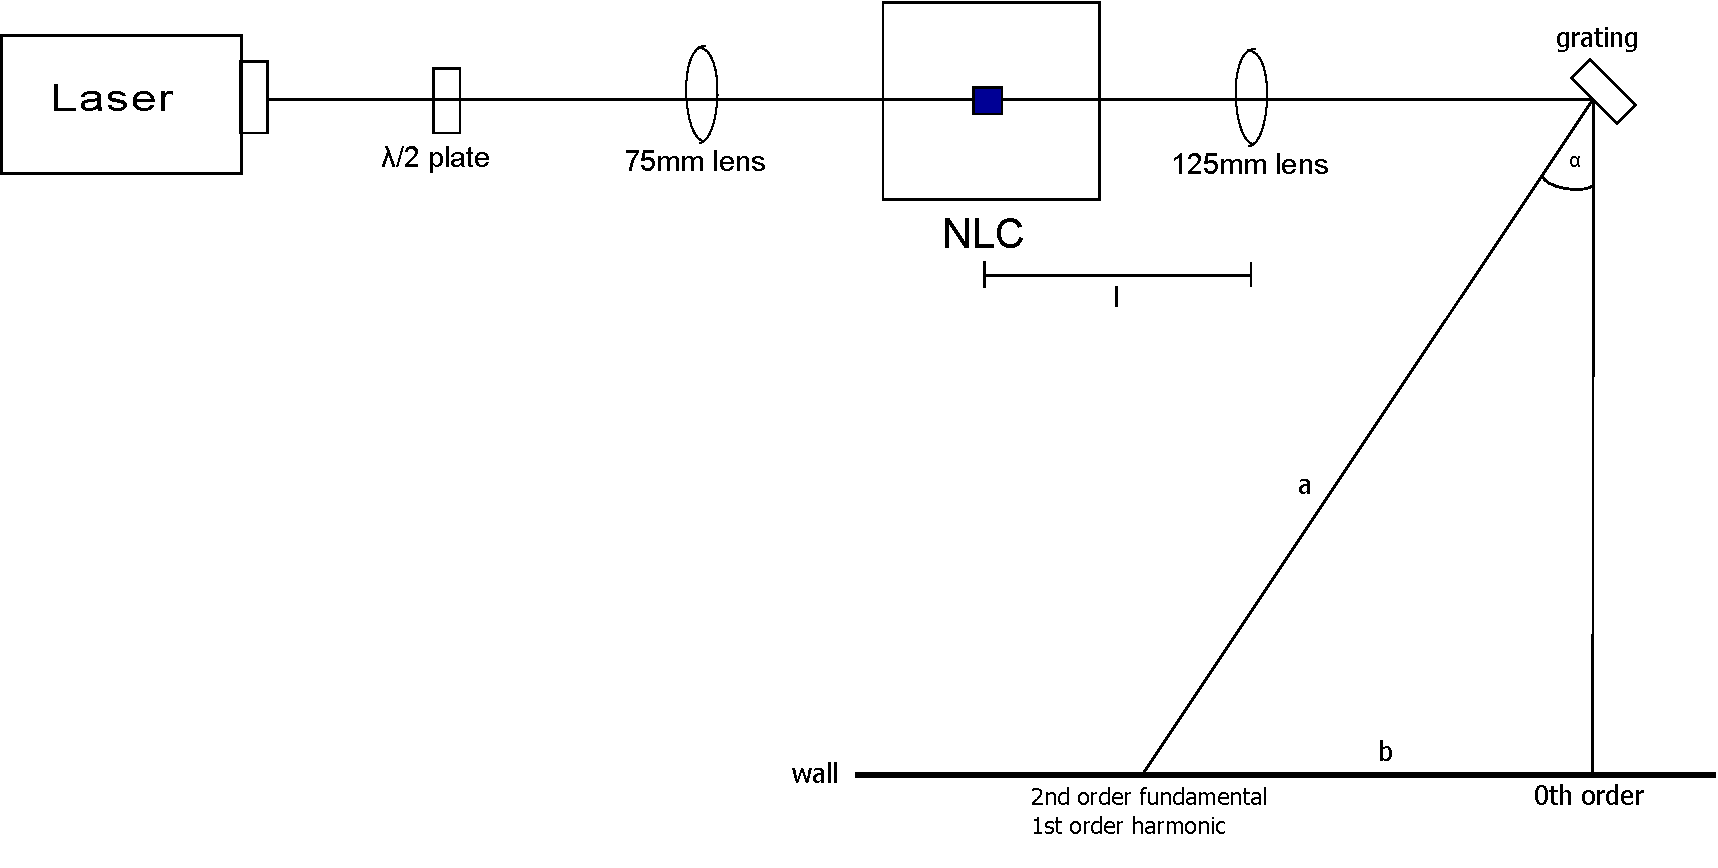
\includegraphics[width=1.0\textwidth]{graphics/setup_grating}
  \caption{Setup of the experiment for wavelength analysis with grating}
  \label{fig:setup_grating}
\end{figure}
For diffraction gratings the following equations hold:
\begin{align*}
\sin \alpha = \frac{m\lambda}{g} \hspace{2cm} \frac{\lambda}{\Delta \lambda} = mN = mg L
\end{align*}
where $m$ is the order of the interference, $g$ is the grating constant, $N$ the number of "slits" illuminated and $L$ is the width of the incoming beam at the grating. In our case $g = \unit[600]{Lines/mm}$ and the width of the beam may be approximated via 
\begin{align*}
L = 2\frac{\omega_{0,\textrm{f}}}{f}l
\end{align*}
where we assumed that the beam is completely collimated behind the 125mm achromatic lens and we adjusted the lens that way that $l = \unit[(130 \pm 5)]{mm}$ holds. So the theoretical spectral resolution is given by:
\begin{align}
\left(\frac{\lambda}{\Delta\lambda}\right)_\textrm{th} = 2mg\frac{\omega_{0,\textrm{f}}}{f}l \hspace{1.5cm} \Delta\left(\frac{\lambda}{\Delta\lambda}\right)_\textrm{th} = \sqrt{\left(2mg\frac{l}{f}\omega_{0,\textrm{f}}\Delta \right)^2+\left(2mg\frac{\omega_{0,\textrm{f}}}{f}\Delta l\right)^2}
\end{align}
plugging in the values yields:
\begin{align}
\left(\frac{\lambda}{\Delta\lambda}\right)_\textrm{th} = \unit[(7280 \pm 3875)]{}
\end{align}
The error of the theoretical spectral resolution is relatively big. This is caused by the large uncertainty in the size of $l$, which has such a large value because we removed the achromatic lens after having measured the distance to improve the beam collimation and forgot to remeasure the distance.

To determine the experimental spectral resolution and the wavelengths of the beams we measure:
\begin{align}
a &= \unit[(193.4 \pm 0.1)]{cm}\\
\notag b_\textrm{f} &= b_\textrm{h} = \unit[(120.3 \pm 0.1)]{cm}% \hspace{3cm} \textrm{(fundamental wave)}\\
%\notag b_\textrm{h} &= \unit[(120.3 \pm 2.4)]{cm} \hspace{3cm} \textrm{(harmonic wave)}
\end{align}
For the wavelengths, the ratio of wavelengths and the spectral resolution we get
\begin{align*}
\lambda_i &= \frac{\sin\alpha_i}{m_ig}\hspace{2cm}\Delta \lambda_i = \frac{\Delta\sin\alpha_i}{m_ig}\\
\frac{\lambda_\textrm{f}}{\lambda_\textrm{h}} &= 2 \frac{\sin\alpha_\textrm{f}}{\sin\alpha_\textrm{h}}\hspace{2cm} \Delta\frac{\lambda_\textrm{f}}{\lambda_\textrm{h}} = 2\sqrt{\left(\frac{\Delta\sin\alpha_\textrm{f}}{\sin\alpha_\textrm{h}}\right)^2+\left(\frac{\sin\alpha_\textrm{f}\Delta\sin\alpha_\textrm{h}}{\sin^2\alpha_\textrm{h}}\right)^2}\\
\frac{\lambda}{\Delta \lambda}&=\frac{\sin\alpha}{\Delta\sin\alpha}
\end{align*}
where
\begin{align*}
\sin\alpha_i = \frac{b_i}{a}\hspace{2cm}\Delta \sin\alpha_i=\sqrt{\left(\frac{\Delta b_i}{a}\right)^2+\left(\frac{b_i\Delta a}{a^2}\right)^2}
\end{align*}
and $i \in \{h,f\}$. Plugging in our values we get:
\begin{align}
\lambda_\textrm{f}&=\unit[(1037 \pm 1)]{nm} \\
 \lambda_\textrm{h}&=\unit[(518.4 \pm 0.5)]{nm}\\
\frac{\lambda_\textrm{f}}{\lambda_\textrm{h}} &= \unit[(2.000 \pm 0.003)]{}\\
\frac{\lambda}{\Delta \lambda} &\approx \unit[1022]{}
\end{align}
Our experimental resolution is therefore clearly smaller than the theoretical one. That is caused at most by the relatively large size of the spots on the wall and therefore a big error on the value of $b$.
\subsubsection{Analysis with \textsc{Michelson} interferometer}\label{subsubsec:ana_michelson}
a
\section{Abstract}

\begin{appendix}
\section{Figures}

\section{Tables}
\begin{table}[H]
  \centering
\resizebox{0.8\textwidth}{!}{
  \begin{tabular}{lcccc}
    \toprule
      $I$ [$\unit[]{mA}$] $\pm$ $\unit[0.5]{mA}$ & $P$ [$\unit[]{\mu W}$]  &  $P_\textrm{background}$ [$\unit[]{\mu W}$] & $\Delta P$ [$\unit[]{\mu W}$]\\
    \midrule[0.75pt]
$1$ & $0.000$ & $0.001$ & $0.001$\\
$11$ & $0.001$ & $0.001$ & $0.001$\\
$20$ & $0.001$ & $0.001$ & $0.001$\\
$30$ & $0.001$ & $0.001$ & $0.001$\\
$40$ & $0.002$ & $0.001$ & $0.001$\\
$45$ & $0.003$ & $0.001$ & $0.001$\\
$50$ & $0.003$ & $0.001$ & $0.001$\\
$55$ & $0.004$ & $0.001$ & $0.001$\\
$60$ & $0.610$ & $0.001$ & $0.001$\\
$65$ & $3.33$ & $0.01$ & $0.01$\\
$70$ & $6.34$ & $0.01$ & $0.01$\\
$75$ & $9.58$ & $0.01$ & $0.01$\\
$80$ & $12.9$ & $0.1$ & $0.1$\\
$90$ & $16.5$ & $0.1$ & $0.1$\\
$100$ & $24.9$ & $0.1$ & $0.1$\\
$110$ & $28.4$ & $0.1$ & $0.1$\\
$120$ & $35.4$ & $0.1$ & $0.1$\\
$130$ & $41.0$ & $0.1$ & $0.1$\\
$140$ & $46.0$ & $0.1$ & $0.1$\\
$150$ & $52.0$ & $0.1$ & $0.1$\\
$160$ & $58.5$ & $0.1$ & $0.1$\\
$170$ & $64.0$ & $0.1$ & $0.1$\\
$180$ & $69.8$ & $0.1$ & $0.1$\\
$190$ & $75.7$ & $0.1$ & $0.1$\\
$200$ & $79.9$ & $0.1$ & $0.1$\\
$210$ & $86.0$ & $0.1$ & $0.1$\\
$220$ & $90.3$ & $0.1$ & $0.1$\\
$230$ & $98.0$ & $0.1$ & $0.1$\\
$240$ & $104$ & $1$ & $1$\\
$250$ & $112$ & $1$ & $1$\\
$260$ & $114$ & $1$ & $1$\\
$270$ & $124$ & $1$ & $1$\\
$280$ & $126$ & $1$ & $1$\\
    \bottomrule
  \end{tabular}
}
\caption{Measured laser power for different input currents with attenuator}
  \label{tab:ana_laserpower_att}
\end{table}
\begin{table}[H]
  \centering
\resizebox{0.8\textwidth}{!}{
  \begin{tabular}{lcccc}
    \toprule
      $I$ [$\unit[]{mA}$] $\pm$ $\unit[0.5]{mA}$ & $P$ [$\unit[]{mW}$]  &  $P_\textrm{background}$ [$\unit[]{mW}$] & $\Delta P$ [$\unit[]{mW}$]\\
    \midrule[0.75pt]
$60$ & $0.65$ & $0.00$ & $0.01$\\
$65$ & $3.07$ & $0.00$ & $0.01$\\
$70$ & $5.56$ & $0.00$ & $0.01$\\
$75$ & $9.08$ & $0.00$ & $0.01$\\
$80$ & $12.2$ & $0.0$ & $0.1$\\
$85$ & $14.5$ & $0.0$ & $0.1$\\
$90$ & $17.4$ & $0.0$ & $0.1$\\
$95$ & $21.4$ & $0.0$ & $0.1$\\
$100$ & $24.2$ & $0.0$ & $0.1$\\
    \bottomrule
  \end{tabular}
}
\caption{Measured laser power for different input currents without attenuator}
  \label{tab:ana_laserpower_woatt}
\end{table}

\begin{table}[H]
  \centering
\begin{floatrow}
\footnotesize
\resizebox{0.33\textwidth}{!}{
  \begin{tabular}{lcc}
    \toprule
      $\Phi$ [$\unit[]{�}$] $\pm$ $\unit[1]{�}$ & $P_\textrm{attenuated}$ [$\unit[]{mW}$]\\
    \midrule[0.75pt]
$0.0$ & $118.0 \pm 1.0$ \\
$2.5$ & $115.0 \pm 1.0$ \\
$5.0$ & $113.0 \pm 1.0$ \\
$7.5$ & $107.0 \pm 1.0$ \\
$10.0$ & $101.0 \pm 1.0$ \\
$12.5$ & $94.0 \pm 1.0$ \\
$15.0$ & $85.0 \pm 1.0$ \\
$17.5$ & $75.0 \pm 1.0$ \\
$20.0$ & $65.0 \pm 1.0$ \\
$22.5$ & $55.0 \pm 1.0$ \\
$25.0$ & $46.0 \pm 1.0$ \\
$27.5$ & $36.0 \pm 1.0$ \\
$30.0$ & $26.0 \pm 1.0$ \\
$32.5$ & $20.0 \pm 1.0$ \\
$35.0$ & $13.0 \pm 1.0$ \\
$37.5$ & $7.0 \pm 0.1$ \\
$40.0$ & $3.0 \pm 0.1$ \\
$42.5$ & $0.8 \pm 0.1$ \\
$45.0$ & $0.34 \pm 0.01$ \\
$47.5$ & $1.5 \pm 0.1$ \\
$50.0$ & $4.8 \pm 0.1$ \\
$52.5$ & $8.8 \pm 0.1$ \\
$55.0$ & $16.0 \pm 1.0$ \\
$57.5$ & $23.0 \pm 1.0$ \\
$60.0$ & $32.0 \pm 1.0$ \\
$62.5$ & $41.0 \pm 1.0$ \\
$65.0$ & $51.0 \pm 1.0$ \\
$67.5$ & $61.0 \pm 1.0$ \\
$70.0$ & $72.0 \pm 1.0$ \\
$72.5$ & $80.0 \pm 1.0$ \\
$75.0$ & $90.0 \pm 1.0$ \\
    \bottomrule
  \end{tabular}
}
\resizebox{0.33\textwidth}{!}{
  \begin{tabular}{lcc}
    \toprule
      $\Phi$ [$\unit[]{�}$] $\pm$ $\unit[1]{�}$ & $P_\textrm{attenuated}$ [$\unit[]{mW}$]\\
    \midrule[0.75pt]
$77.5$ & $97.0 \pm 1.0$ \\
$80.0$ & $105.0 \pm 1.0$ \\
$82.5$ & $110.0 \pm 1.0$ \\
$85.0$ & $115.0 \pm 1.0$ \\
$87.5$ & $117.0 \pm 1.0$ \\
$90.0$ & $117.0 \pm 1.0$ \\
$92.5$ & $116.0 \pm 1.0$ \\
$95.0$ & $113.0 \pm 1.0$ \\
$97.5$ & $109.0 \pm 1.0$ \\
$100.0$ & $102.0 \pm 1.0$ \\
$102.5$ & $95.0 \pm 1.0$ \\
$105.0$ & $87.0 \pm 1.0$ \\
$107.5$ & $78.0 \pm 1.0$ \\
$110.0$ & $67.0 \pm 1.0$ \\
$112.5$ & $58.0 \pm 1.0$ \\
$115.0$ & $46.0 \pm 1.0$ \\
$117.5$ & $39.0 \pm 1.0$ \\
$120.0$ & $28.0 \pm 1.0$ \\
$122.5$ & $21.0 \pm 1.0$ \\
$125.0$ & $13.0 \pm 1.0$ \\
$127.5$ & $8.0 \pm 0.1$ \\
$130.0$ & $4.0 \pm 0.1$ \\
$132.5$ & $2.0 \pm 0.1$ \\
$135.0$ & $0.80 \pm 0.01$ \\
$137.5$ & $1.9 \pm 0.1$ \\
$140.0$ & $5.0 \pm 0.1$ \\
$142.5$ & $9.0 \pm 0.1$ \\
$145.0$ & $16.0 \pm 1.0$ \\
$147.5$ & $22.0 \pm 1.0$ \\
$150.0$ & $31.0 \pm 1.0$ \\
    \bottomrule
  \end{tabular}
}
\resizebox{0.33\textwidth}{!}{
  \begin{tabular}{lcc}
    \toprule
      $\Phi$ [$\unit[]{�}$] $\pm$ $\unit[1]{�}$ & $P_\textrm{attenuated}$ [$\unit[]{mW}$]\\
    \midrule[0.75pt]
$152.5$ & $40.0 \pm 1.0$ \\
$155.0$ & $50.0 \pm 1.0$ \\
$157.5$ & $60.0 \pm 1.0$ \\
$160.0$ & $71.0 \pm 1.0$ \\
$162.5$ & $80.0 \pm 1.0$ \\
$165.0$ & $90.0 \pm 1.0$ \\
$167.5$ & $97.0 \pm 1.0$ \\
$170.0$ & $106.0 \pm 1.0$ \\
$172.5$ & $111.0 \pm 1.0$ \\
$175.0$ & $115.0 \pm 1.0$ \\
$177.5$ & $117.0 \pm 1.0$ \\
$180.0$ & $118.0 \pm 1.0$ \\
$182.5$ & $117.0 \pm 1.0$ \\
$185.0$ & $113.0 \pm 1.0$ \\
$187.5$ & $110.0 \pm 1.0$ \\
$190.0$ & $102.0 \pm 1.0$ \\
$192.5$ & $96.0 \pm 1.0$ \\
$195.0$ & $86.0 \pm 1.0$ \\
$197.5$ & $78.0 \pm 1.0$ \\
$200.0$ & $67.0 \pm 1.0$ \\
$202.5$ & $58.0 \pm 1.0$ \\
$205.0$ & $46.0 \pm 1.0$ \\
$207.5$ & $39.0 \pm 1.0$ \\
$210.0$ & $28.0 \pm 1.0$ \\
$212.5$ & $20.0 \pm 1.0$ \\
$215.0$ & $13.0 \pm 1.0$ \\
$217.5$ & $8.0 \pm 0.1$ \\
$220.0$ & $4.0 \pm 0.1$ \\
$222.5$ & $1.0 \pm 0.1$ \\
$225.0$ & $0.40 \pm 0.01$ \\
    \bottomrule
  \end{tabular}
}
\end{floatrow}
\caption{Transmission of the variable attenuator depending on the rotation angle of the $\lambda / 2$ plate}
  \label{tab:ana_var_att}
\end{table}

\begin{table}[H]
  \centering
\begin{floatrow}
\footnotesize
\resizebox{0.5\textwidth}{!}{
  \begin{tabular}{lccc}
    \toprule
      $T$ [$\unit[]{�C}$] & $P$ [$\unit[]{\mu W}$] &  $P_\textrm{bgr}$ [$\unit[]{\mu W}$] &  $\Delta P$ [$\unit[]{\mu W}$]\\
    \midrule[0.75pt]
$27.0 \pm 0.1$ & $1.87$ & $0.24$ & $0.01$ \\
$27.2 \pm 0.1$ & $1.86$ & $0.24$ & $0.01$ \\
$27.4 \pm 0.1$ & $1.87$ & $0.24$ & $0.01$ \\
$27.6 \pm 0.1$ & $1.88$ & $0.24$ & $0.01$ \\
$27.8 \pm 0.1$ & $1.88$ & $0.24$ & $0.01$ \\
$28.0 \pm 0.1$ & $1.88$ & $0.24$ & $0.01$ \\
$28.2 \pm 0.1$ & $1.87$ & $0.24$ & $0.01$ \\
$28.4 \pm 0.1$ & $1.87$ & $0.24$ & $0.01$ \\
$28.6 \pm 0.1$ & $1.87$ & $0.24$ & $0.01$ \\
$28.8 \pm 0.1$ & $1.88$ & $0.24$ & $0.01$ \\
$29.0 \pm 0.1$ & $1.90$ & $0.24$ & $0.01$ \\
$29.2 \pm 0.1$ & $1.90$ & $0.24$ & $0.01$ \\
$29.4 \pm 0.1$ & $1.89$ & $0.24$ & $0.01$ \\
$29.6 \pm 0.1$ & $1.88$ & $0.24$ & $0.01$ \\
$29.8 \pm 0.1$ & $1.87$ & $0.24$ & $0.01$ \\
$30.0 \pm 0.1$ & $1.88$ & $0.24$ & $0.01$ \\
$30.2 \pm 0.1$ & $1.90$ & $0.24$ & $0.01$ \\
$30.4 \pm 0.1$ & $1.92$ & $0.24$ & $0.01$ \\
$30.6 \pm 0.1$ & $1.92$ & $0.24$ & $0.01$ \\
$30.8 \pm 0.1$ & $1.92$ & $0.22$ & $0.01$ \\
$31.0 \pm 0.1$ & $1.88$ & $0.22$ & $0.01$ \\
$31.2 \pm 0.1$ & $1.87$ & $0.22$ & $0.01$ \\
$31.4 \pm 0.1$ & $1.89$ & $0.22$ & $0.01$ \\
$31.6 \pm 0.1$ & $1.92$ & $0.22$ & $0.01$ \\
$31.8 \pm 0.1$ & $1.95$ & $0.22$ & $0.01$ \\
$32.0 \pm 0.1$ & $1.94$ & $0.22$ & $0.01$ \\
$32.2 \pm 0.1$ & $1.91$ & $0.22$ & $0.01$ \\
$32.4 \pm 0.1$ & $1.88$ & $0.22$ & $0.01$ \\
$32.6 \pm 0.1$ & $1.89$ & $0.22$ & $0.01$ \\
$32.8 \pm 0.1$ & $1.94$ & $0.22$ & $0.01$ \\
$33.0 \pm 0.1$ & $2.01$ & $0.22$ & $0.01$ \\
$33.2 \pm 0.1$ & $2.03$ & $0.22$ & $0.01$ \\
$33.4 \pm 0.1$ & $2.01$ & $0.22$ & $0.01$ \\
    \bottomrule
  \end{tabular}
}
\resizebox{0.5\textwidth}{!}{
  \begin{tabular}{lccc}
    \toprule
      $T$ [$\unit[]{�C}$] & $P$ [$\unit[]{\mu W}$] &  $P_\textrm{bgr}$ [$\unit[]{\mu W}$] &  $\Delta P$ [$\unit[]{\mu W}$]\\
    \midrule[0.75pt]
$33.6 \pm 0.1$ & $1.95$ & $0.22$ & $0.01$ \\
$33.8 \pm 0.1$ & $1.94$ & $0.22$ & $0.01$ \\
$34.0 \pm 0.1$ & $2.00$ & $0.22$ & $0.01$ \\
$34.2 \pm 0.1$ & $2.09$ & $0.22$ & $0.01$ \\
$34.4 \pm 0.1$ & $2.14$ & $0.22$ & $0.01$ \\
$34.6 \pm 0.1$ & $2.13$ & $0.22$ & $0.01$ \\
$34.8 \pm 0.1$ & $2.19$ & $0.22$ & $0.01$ \\
$35.0 \pm 0.1$ & $2.79$ & $0.22$ & $0.01$ \\
$35.2 \pm 0.1$ & $4.58$ & $0.22$ & $0.01$ \\
$35.4 \pm 0.1$ & $7.60$ & $0.22$ & $0.01$ \\
$35.6 \pm 0.1$ & $12.8$ & $0.30$ & $0.1$ \\
$35.8 \pm 0.1$ & $18.9$ & $0.30$ & $0.1$ \\
$36.0 \pm 0.1$ & $23.5$ & $0.30$ & $0.1$ \\
$36.2 \pm 0.1$ & $26.9$ & $0.30$ & $0.1$ \\
$36.4 \pm 0.1$ & $27.6$ & $0.30$ & $0.1$ \\
$36.6 \pm 0.1$ & $24.0$ & $0.30$ & $0.1$ \\
$36.8 \pm 0.1$ & $20.7$ & $0.30$ & $0.1$ \\
$37.0 \pm 0.1$ & $13.9$ & $0.30$ & $0.1$ \\
$37.2 \pm 0.1$ & $8.3$ & $0.30$ & $0.1$ \\
$37.4 \pm 0.1$ & $4.5$ & $0.30$ & $0.1$ \\
$37.6 \pm 0.1$ & $2.8$ & $0.30$ & $0.1$ \\
$37.8 \pm 0.1$ & $2.2$ & $0.30$ & $0.1$ \\
$38.0 \pm 0.1$ & $2.5$ & $0.30$ & $0.1$ \\
$38.2 \pm 0.1$ & $2.7$ & $0.30$ & $0.1$ \\
$38.4 \pm 0.1$ & $2.7$ & $0.30$ & $0.1$ \\
$38.6 \pm 0.1$ & $2.4$ & $0.30$ & $0.1$ \\
$38.8 \pm 0.1$ & $2.1$ & $0.30$ & $0.1$ \\
$39.0 \pm 0.1$ & $1.9$ & $0.30$ & $0.1$ \\
$39.2 \pm 0.1$ & $2.0$ & $0.30$ & $0.1$ \\
$39.4 \pm 0.1$ & $2.1$ & $0.30$ & $0.1$ \\
$39.6 \pm 0.1$ & $2.1$ & $0.30$ & $0.1$ \\
$39.8 \pm 0.1$ & $2.1$ & $0.30$ & $0.1$ \\
$40.0 \pm 0.1$ & $2.0$ & $0.30$ & $0.1$ \\
    \bottomrule
  \end{tabular}
}
\end{floatrow}
\caption{Power of the second harmonic generation for different NLC temperatures}
  \label{tab:ana_temp_dep}
\end{table}

\begin{table}[H]
  \centering
\resizebox{0.8\textwidth}{!}{
  \begin{tabular}{lccccc}
    \toprule
      $\Phi$ [$\unit[]{�}$] $\pm$ $\unit[1]{�}$ & $P_\textrm{fun}$ [$\unit[]{mW}$]  &  $P_\textrm{harm}$ [$\unit[]{\mu W}$] & $P_\textrm{bgr}$ [$\unit[]{\mu W}$] & $\Delta P$ [$\unit[]{\mu W}$]\\
    \midrule[0.75pt]
$0.0$ & $112.6 \pm 0.4$ & $23.7$ & $0.01$ & $0.1$\\
$2.5$ & $111.7 \pm 0.8$ & $23.0$ & $0.01$ & $0.1$\\
$5.0$ & $109 \pm 1$ & $21.4$ & $0.01$ & $0.1$\\
$7.5$ & $105 \pm 2$ & $19.6$ & $0.01$ & $0.1$\\
$10.0$ & $99 \pm 3$ & $17.5$ & $0.01$ & $0.1$\\
$12.5$ & $92 \pm 3$ & $15.3$ & $0.01$ & $0.1$\\
$15.0$ & $84 \pm 3$ & $12.6$ & $0.01$ & $0.1$\\
$17.5$ & $75 \pm 4$ & $9.9$ & $0.01$ & $0.01$\\
$20.0$ & $66 \pm 4$ & $7.0$ & $0.01$ & $0.01$\\
$22.5$ & $56 \pm 4$ & $5.2$ & $0.01$ & $0.01$\\
$25.0$ & $46 \pm 4$ & $3.5$ & $0.01$ & $0.01$\\
$27.5$ & $37 \pm 4$ & $2.3$ & $0.01$ & $0.01$\\
$30.0$ & $28 \pm 3$ & $1.3$ & $0.01$ & $0.01$\\
$32.5$ & $20 \pm 3$ & $0.8$ & $0.01$ & $0.01$\\
$35.0$ & $13 \pm 3$ & $0.4$ & $0.01$ & $0.01$\\
$37.5$ & $7 \pm 2$ & $0.2$ & $0.01$ & $0.01$\\
$40.0$ & $3 \pm 1$ & $0.11$ & $0.01$ & $0.01$\\
$42.5$ & $0.8 \pm 0.7$ & $0.09$ & $0.01$ & $0.01$\\
$45.0$ & $0.0 \pm 0.0$ & $0.09$ & $0.01$ & $0.01$\\
    \bottomrule
  \end{tabular}
}
\caption{Power of the second harmonic generation for different rotation angles of the $\lambda / 2$ plate (with analyzer built in) and therefore different incoming laser power, with corresponding fundamental wave power}
  \label{tab:ana_power_dep}
\end{table}

\begin{table}[H]
  \centering
\footnotesize
\begin{floatrow}
\resizebox{0.5\textwidth}{!}{
  \begin{tabular}{lcccc}
    \toprule
      $\Phi$ [$\unit[]{�}$]& $P$ [$\unit[]{\mu W}$]  &  $P_\textrm{bgr}$ [$\unit[]{\mu W}$] & $\Delta P$ [$\unit[]{\mu W}$]\\
    \midrule[0.75pt]
$0.0 \pm 0.1$ & $32.0$ & $0.2$ & $0.1$\\
$2.5 \pm 0.1$ & $28.5$ & $0.2$ & $0.1$\\
$5.0 \pm 0.1$ & $27.1$ & $0.2$ & $0.1$\\
$7.5 \pm 0.1$ & $24.8$ & $0.2$ & $0.1$\\
$10.0 \pm 0.1$ & $22.0$ & $0.2$ & $0.1$\\
$12.5 \pm 0.1$ & $19.4$ & $0.2$ & $0.1$\\
$15.0 \pm 0.1$ & $15.7$ & $0.2$ & $0.1$\\
$17.5 \pm 0.1$ & $12.6$ & $0.2$ & $0.1$\\
$20.0 \pm 0.1$ & $9.9$ & $0.2$ & $0.1$\\
$22.5 \pm 0.1$ & $7.7$ & $0.2$ & $0.1$\\
$25.0 \pm 0.1$ & $5.6$ & $0.2$ & $0.1$\\
$27.5 \pm 0.1$ & $4.3$ & $0.2$ & $0.1$\\
$30.0 \pm 0.1$ & $3.2$ & $0.2$ & $0.1$\\
$32.5 \pm 0.1$ & $2.4$ & $0.2$ & $0.1$\\
$35.0 \pm 0.1$ & $2.0$ & $0.2$ & $0.1$\\
$37.5 \pm 0.1$ & $1.8$ & $0.2$ & $0.1$\\
$40.0 \pm 0.1$ & $1.8$ & $0.2$ & $0.1$\\
$42.5 \pm 0.1$ & $1.7$ & $0.2$ & $0.1$\\
$45.0 \pm 0.1$ & $1.7$ & $0.2$ & $0.1$\\
$47.5 \pm 0.1$ & $1.8$ & $0.2$ & $0.1$\\
$50.0 \pm 0.1$ & $1.8$ & $0.2$ & $0.1$\\
$52.5 \pm 0.1$ & $1.9$ & $0.2$ & $0.1$\\
$55.0 \pm 0.1$ & $2.1$ & $0.2$ & $0.1$\\
$57.5 \pm 0.1$ & $2.6$ & $0.2$ & $0.1$\\
$60.0 \pm 0.1$ & $3.5$ & $0.2$ & $0.1$\\
$62.5 \pm 0.1$ & $4.7$ & $0.2$ & $0.1$\\
$65.0 \pm 0.1$ & $6.3$ & $0.2$ & $0.1$\\
$67.5 \pm 0.1$ & $8.1$ & $0.2$ & $0.1$\\
$70.0 \pm 0.1$ & $10.7$ & $0.2$ & $0.1$\\
$72.5 \pm 0.1$ & $12.6$ & $0.2$ & $0.1$\\
$75.0 \pm 0.1$ & $15.7$ & $0.2$ & $0.1$\\
$77.5 \pm 0.1$ & $17.9$ & $0.2$ & $0.1$\\
$80.0 \pm 0.1$ & $20.6$ & $0.2$ & $0.1$\\
$82.5 \pm 0.1$ & $22.6$ & $0.2$ & $0.1$\\
$85.0 \pm 0.1$ & $23.8$ & $0.2$ & $0.1$\\
$87.5 \pm 0.1$ & $24.4$ & $0.2$ & $0.1$\\
$90.0 \pm 0.1$ & $24.3$ & $0.2$ & $0.1$\\
$92.5 \pm 0.1$ & $23.6$ & $0.2$ & $0.1$\\
$95.0 \pm 0.1$ & $22.3$ & $0.2$ & $0.1$\\
    \bottomrule
  \end{tabular}
}
\resizebox{0.5\textwidth}{!}{
  \begin{tabular}{lcccc}
    \toprule
      $\Phi$ [$\unit[]{�}$]& $P$ [$\unit[]{\mu W}$]  &  $P_\textrm{bgr}$ [$\unit[]{\mu W}$] & $\Delta P$ [$\unit[]{\mu W}$]\\
    \midrule[0.75pt]
$97.5 \pm 0.1$ & $20.6$ & $0.2$ & $0.1$\\
$100.0 \pm 0.1$ & $18.2$ & $0.2$ & $0.1$\\
$102.5 \pm 0.1$ & $15.7$ & $0.2$ & $0.1$\\
$105.0 \pm 0.1$ & $14.5$ & $0.2$ & $0.1$\\
$107.5 \pm 0.1$ & $11.2$ & $0.2$ & $0.1$\\
$110.0 \pm 0.1$ & $8.5$ & $0.2$ & $0.1$\\
$112.5 \pm 0.1$ & $6.8$ & $0.2$ & $0.1$\\
$115.0 \pm 0.1$ & $5.1$ & $0.2$ & $0.1$\\
$117.5 \pm 0.1$ & $3.9$ & $0.2$ & $0.1$\\
$120.0 \pm 0.1$ & $2.8$ & $0.2$ & $0.1$\\
$122.5 \pm 0.1$ & $2.3$ & $0.2$ & $0.1$\\
$125.0 \pm 0.1$ & $1.9$ & $0.2$ & $0.1$\\
$127.5 \pm 0.1$ & $1.7$ & $0.2$ & $0.1$\\
$130.0 \pm 0.1$ & $1.7$ & $0.2$ & $0.1$\\
$132.5 \pm 0.1$ & $1.6$ & $0.2$ & $0.1$\\
$135.0 \pm 0.1$ & $1.6$ & $0.2$ & $0.1$\\
$137.5 \pm 0.1$ & $1.7$ & $0.2$ & $0.1$\\
$140.0 \pm 0.1$ & $1.7$ & $0.2$ & $0.1$\\
$142.5 \pm 0.1$ & $1.8$ & $0.2$ & $0.1$\\
$145.0 \pm 0.1$ & $2.0$ & $0.2$ & $0.1$\\
$147.5 \pm 0.1$ & $2.4$ & $0.2$ & $0.1$\\
$150.0 \pm 0.1$ & $3.4$ & $0.2$ & $0.1$\\
$152.5 \pm 0.1$ & $4.3$ & $0.2$ & $0.1$\\
$155.0 \pm 0.1$ & $6.1$ & $0.2$ & $0.1$\\
$157.5 \pm 0.1$ & $7.8$ & $0.2$ & $0.1$\\
$160.0 \pm 0.1$ & $10.3$ & $0.2$ & $0.1$\\
$162.5 \pm 0.1$ & $13.0$ & $0.2$ & $0.1$\\
$165.0 \pm 0.1$ & $15.6$ & $0.2$ & $0.1$\\
$167.5 \pm 0.1$ & $18.0$ & $0.2$ & $0.1$\\
$170.0 \pm 0.1$ & $20.9$ & $0.2$ & $0.1$\\
$172.5 \pm 0.1$ & $22.6$ & $0.2$ & $0.1$\\
$175.0 \pm 0.1$ & $24.1$ & $0.2$ & $0.1$\\
$177.5 \pm 0.1$ & $25.1$ & $0.2$ & $0.1$\\
$180.0 \pm 0.1$ & $25.4$ & $0.2$ & $0.1$\\
$182.5 \pm 0.1$ & $25.1$ & $0.2$ & $0.1$\\
$185.0 \pm 0.1$ & $23.6$ & $0.2$ & $0.1$\\
$187.5 \pm 0.1$ & $22.0$ & $0.2$ & $0.1$\\
$190.0 \pm 0.1$ & $19.5$ & $0.2$ & $0.1$\\
\bottomrule
\end{tabular}
}
\end{floatrow}
\caption{Power of the second harmonic generation for different rotation angles of the $\lambda / 2$ plate (without analyzer) and therefore different incoming wave polarizations, with corresponding fundamental wave power}
  \label{tab:ana_pol_dep}
\end{table}
\Literatur{quellen}

\end{appendix}
\end{document}


